%TC: macro \marginfootnote [other]
%TC: envir SCfigure [] other
%TC: macrocount beginSCfigure [figure]
\documentclass[11pt,twoside]{report}
\usepackage{preamble}
\usepackage{standalone}
\graphicspath{{../img/}}

\DeclareRobustCommand{\wordcount}{%TC: macro \marginfootnote [other]
%TC: envir SCfigure [] other
%TC: macrocount beginSCfigure [figure]
\documentclass[11pt,twoside]{report}
\usepackage{preamble}
\usepackage{standalone}
\graphicspath{{../img/}}

\DeclareRobustCommand{\wordcount}{%TC: macro \marginfootnote [other]
%TC: envir SCfigure [] other
%TC: macrocount beginSCfigure [figure]
\documentclass[11pt,twoside]{report}
\usepackage{preamble}
\usepackage{standalone}
\graphicspath{{../img/}}

\DeclareRobustCommand{\wordcount}{%TC: macro \marginfootnote [other]
%TC: envir SCfigure [] other
%TC: macrocount beginSCfigure [figure]
\documentclass[11pt,twoside]{report}
\usepackage{preamble}
\usepackage{standalone}
\graphicspath{{../img/}}

\DeclareRobustCommand{\wordcount}{\input{thesis.wordcountsum}}
\definecolor{bristolred}{RGB}{191,47,56}

\begin{document}

\newgeometry{margin=1in}

%\maketitle
\thispagestyle{empty}
\begin{center}
  \begin{minipage}{0.8\linewidth}
    \centering
    %
\includegraphics[width=0.6\linewidth]{bristol-logo}\par
    %\rule{0.4\linewidth}{0.15\linewidth}\par
    \vspace{3cm}
    %\hline
    {\Large \sc University of Bristol \par}
    \vspace{2cm}
    {\Large \sc Doctoral Thesis \par}
    \vspace{1cm}
    \rule{\textwidth}{0.4pt} \par
    {\LARGE \sc \color{bristolred} Some equilibrium approaches to the high-density liquid (working title) \par}
    \rule{\textwidth}{0.4pt} \par
    %\hline
    \vspace{2cm}
    {\large \it Author:}
    \hfill
    {\large \it Supervisor:} \\
    {\sc \large \href{mailto:joshua.robinson@bristol.ac.uk}{Joshua F.\ Robinson}}
    \hfill
    {\sc \large Prof.\ C.\ P.\ Royall \par}
    \vspace{3.5cm}
   {\large \it A dissertation submitted to the University of Bristol in accordance with the requirements for award of the degree of Doctor of Philosophy in the Faculty of Science, H.\ H.\ Wills Physics Laboratory. \par}
    \vspace{1em}
    {\large August 2019 \par}
  \end{minipage}
  \mbox{}
  \vfill
  \begin{minipage}{0.8\linewidth}
    \raggedleft
    {\large \wordcount words}
  \end{minipage}
\end{center}

\pagenumbering{roman}
\cleardoublepage\include{abstract}
\cleardoublepage\include{dedication}
\cleardoublepage\include{acknowledgements}
\cleardoublepage\include{declaration}
\cleardoublepage\include{opening-quote}

\cleardoublepage\tableofcontents
\cleardoublepage\listoffigures
\cleardoublepage\listoftodos

\restoregeometry

\pagenumbering{arabic}
\setcounter{page}{1}
\include{introduction}
\include{background}
\include{morphometric-framework}
\include{morphometric-applications}
\include{resummation}
\include{aerosols}
\include{conclusion}

\begin{appendices}
  \include{appendix-spt-singularities}
  \include{appendix-two-spheres}
  \include{appendix-full-geometry}
\end{appendices}

\printbibliography[heading=bibintoc]

\end{document}
}
\definecolor{bristolred}{RGB}{191,47,56}

\begin{document}

\newgeometry{margin=1in}

%\maketitle
\thispagestyle{empty}
\begin{center}
  \begin{minipage}{0.8\linewidth}
    \centering
    %
\includegraphics[width=0.6\linewidth]{bristol-logo}\par
    %\rule{0.4\linewidth}{0.15\linewidth}\par
    \vspace{3cm}
    %\hline
    {\Large \sc University of Bristol \par}
    \vspace{2cm}
    {\Large \sc Doctoral Thesis \par}
    \vspace{1cm}
    \rule{\textwidth}{0.4pt} \par
    {\LARGE \sc \color{bristolred} Some equilibrium approaches to the high-density liquid (working title) \par}
    \rule{\textwidth}{0.4pt} \par
    %\hline
    \vspace{2cm}
    {\large \it Author:}
    \hfill
    {\large \it Supervisor:} \\
    {\sc \large \href{mailto:joshua.robinson@bristol.ac.uk}{Joshua F.\ Robinson}}
    \hfill
    {\sc \large Prof.\ C.\ P.\ Royall \par}
    \vspace{3.5cm}
   {\large \it A dissertation submitted to the University of Bristol in accordance with the requirements for award of the degree of Doctor of Philosophy in the Faculty of Science, H.\ H.\ Wills Physics Laboratory. \par}
    \vspace{1em}
    {\large August 2019 \par}
  \end{minipage}
  \mbox{}
  \vfill
  \begin{minipage}{0.8\linewidth}
    \raggedleft
    {\large \wordcount words}
  \end{minipage}
\end{center}

\pagenumbering{roman}
\cleardoublepage\chapter*{Abstract}
\addcontentsline{toc}{chapter}{Abstract}

This dissertation describes an investigation into methods for advancing understanding of liquids at high densities, where dynamical processes become highly non-trivial.
Specifically, we address structure in supercooled liquids approaching their glass transition, and the kinetics of nucleating the stable cystal phase.
In both cases we describe the liquid using equilibrium physics, even though the system is metastable and not strictly in equilibrium.
The first three results chapters focus on the supercooled liquid, while the final results chapter addresses nucleation.

In the first part comprising three chapters, we combine geometric techniques with liquid state theory to develop an approach for treating complex many-particle local structures inside the bulk hard sphere liquid.
We introduce the \emph{morphometric approach}, a liquid state theory based on integral geometry, as a means of calculating many-body correlation functions.
We argue for the morphometric approach from several routes, and derive multiple specific theories for hard spheres including one suitable for producing accurate correlation functions.
We later derive the morphometric approach for hard spheres from first-principles using the virial series.
This places the approach on more rigorous ground, and suggests routes to extending the theory as part of a controlled expansion.

With the resulting many-body correlation functions, we are able to predict the concentrations of complex many-particle structures in the bulk liquid; these results are of particular relevance to theories of supercooled liquids and glasses.
We find a bimodality in the energy landscape for hard sphere local structures, where fivefold symmetric structures appear lower in free energy than fourfold symmetric structures.
In addition, we develop similar techniques for predicting the thermodynamic barriers to dynamical processes inside the bulk system.
The solution to the overarching problem of predicting structure formation inside a bulk system has potential to advance study of self-assembly, nucleation and protein folding in aqueous environments.

In a final part we address nucleation of salt crystals in drying aerosol droplets, of particular relevance to climate models and industrial spray drying applications.
Treating the droplet in the continuum limit, we solve the diffusion equation with moving boundary conditions.
By comparison with experimental data we are able to assess the accuracy of classical nucleation theory, with mixed success depending on the system.
%% We find it successfully predicts the nucleation kinetics of \ce{NaCl} aerosol droplets but fails for \ce{NaNO3}.
%% We find a complex interplay between inhomogeneity of the droplet concentration profile and droplet temperature affects the nucleation kinetics.

\cleardoublepage\chapter*{}
\vspace*{0.2\textheight}
\begin{center}
\noindent\emph{Dedicated to all of the cats of the internet, whose rheological properties inspired this delve into liquids.}
\end{center}

\cleardoublepage%\restoregeometry

\chapter*{\vspace{-1em} Acknowledgements}
\addcontentsline{toc}{chapter}{Acknowledgements}

First and foremost, I want to thank my supervisor, Paddy, for being the reason that any of this happened at all, for being a crucial check on my natural impulse to be \emph{too} focused on details and for the fact that I now see beautiful (pink) icosahedra everytime I close my eyes.
I thank him for giving me the freedom to develop my ideas, and for his remarkable degree of patience when that led to me studying six particles for four years.

It has now been several years since Paddy gave me the `humble' task of solving the glass transition once and for all.
Having failed spectacularly at this, I hope we can collectively agree that the real glass transition was the friends we made along the way.
In particular, all of the cave-dwellers (and countless mice) of G.39 who survived the water features, two fumigations and Paddy.
The forces of darkness may have stolen our toaster, but they never broke our spirit%
\footnote{After all, we had the science to do that.}.
I will treasure these memories, and your friendship, until the end of my days.
%Honorable mentions to the contriband toaster and the electric fence of Fowey.
%Together we braved the near-total sunlight deprivation, more mice than I care to remember and an incident with an electric fence.
%Special thanks go out to the electic fence which our trip to cornwall.

I owe a great debt to Francesco Turci for dedicating far more time than I deserve to discuss my work.
I honestly don't think I could have done this without his consistent, valuable input throughout.

I would like to express my gratitude to our collaborator Roland Roth, for founding the Bristol's White Bear institute, conjuring up the initial idea for my project with Paddy and providing guidance along the way.
Additionally, I am deeply grateful to our collaborators in chemistry for what turned out to be a fun and fruitful project: Flo Gregson, Rachel Miles and Jonathan Reid.
I especially thank Flo for doing the experiments which made this collaboration possible, and for providing valuable feedback on my initial attempts at describing them in chapter \ref{chapter:aerosols}.

Special thanks go out to Bob Evans, who showed interest in my work from the very beginning, for the many stimulating discussions about liquid state theory over the years.
I must also thank him for the constructive feedback he gave on an early draft of the paper underlying parts of chapters \ref{chapter:morphometric-framework} and \ref{chapter:morphometric-applications}.
I recall he described me as ``completely mad'' afterwards, which I \emph{think} was a compliment, so I must additionally thank him for inadverently suggesting an `insanity defence' to rely upon in my viva.

I am very grateful to the organisers and lecturers at the Boulder School in Condensed Matter and Materials Physics 2017.
This school influenced my development as a statisical physicist in a myriad of ways.
Notably, I found myself referring back to the phenomenological lectures by Gilles Tarjus while writing chapter \ref{chapter:glass}.

Financially, I acknowledge the European Research Council under the FP7 / ERC Grant Agreement No.\ 617266 ``NANOPRS'' and Paddy for finding ways to support me after this ran out.

I have learned that research is an almost constant uphill struggle, with the occasional false summit.
My most heartfelt appreciation goes out to all my friends and colleagues who made the struggle worthwhile.
I would particularly like to thank Kate Oliver, Nick Wood and Max Meissner for keeping me sane in difficult times, and Kirsty Wynne for teaching me perspective and the meaning of a `false summit'.
Last, and certainly not least, I owe my deepest gratitude to all the close friends and family members who were there for me every step along the way.

%\newgeometry{margin=1in}

\cleardoublepage\chapter*{Declaration}
I declare that..

\cleardoublepage\chapter*{}
\vspace*{0.2\textheight}
\begin{center}
\noindent\enquote{\itshape Keep cool, never freeze.}\hspace{1.5cm} \bigbreak

\hspace{1.5cm} -- Hellmann's\textsuperscript{\textregistered} mayonnaise bottle.
\end{center}


\cleardoublepage\tableofcontents
\cleardoublepage\listoffigures
\cleardoublepage\listoftodos

\restoregeometry

\pagenumbering{arabic}
\setcounter{page}{1}
%TC: macro \marginfootnote [other]
%TC: envir SCfigure [] other
%TC: macrocount beginSCfigure [figure]
\documentclass[11pt,twoside]{report}
\usepackage{preamble}
\setcounter{chapter}{0}
\graphicspath{{../img/}}
\def\includebibliography{}

\begin{document}
\chapter{Introduction}
\epigraph{Everything starts somewhere, though many physicists disagree.}{Terry Pratchett, \emph{Hogfather}, (1996).}

\section{Overview}

%Begin with a short (1–2 pages) broader introduction for a general audience: one that my mother could understand so she knows what I’ve been working on all these years.

What precisely is covered by soft matter, and how to properly demarcate, is a matter of some academic debate.
In some sense soft matter can be most easily understood by : it is the science of ``squishy'' things.
The eminent soft matter physicist Wilson Poon describes soft matter as ``liquids with bits'' in them.
A more precise and scientific definition posits that the energy scale is subject to thermal fluctuations.
So e.g.\ chemical bonds break and reform allowing flow, but the physical processes may be arbitrarily more complex than simple liquids.

Soft matter was clearly preceded by liquids, and it is up to the individual whether liquids should be considered as the antecedent to or subsumed by soft matter.
My personal bias is that liquids represent a subset of soft matter, the zeroth order approximation to real systems.

\section{Simple liquids}

Physics is filled with toy models.
The Ising model is the most widely studied magnetic model, and the usual starting point for students learning statistical mechanics/phase transitions particular the critical point where this is \emph{the} model system.

What are simple liquids, with hard spheres at the forefront.
\hl{Hard spheres serve as a good touchstone for some of the fundamental knowns and controversies in liquid state theory and, by extension, soft matter.}
The physicists favourite toy model is the hard sphere liquid.
Interaction potential is the no-overlap condition%
\marginfootnote{I like to imagine them as ideal billiard balls, i.e.\ without any dissipative forces like friction so they continue to bounce off one another forever.}:
\begin{equation}
  U =
  \begin{cases}
    \infty & \; r < \sigma \\
    0 & \; \textrm{otherwise}.
  \end{cases}
\end{equation}
As the potential is everywhere zero or divergent, temperature has no effect on the interactions making this system athermal.
Instead, the natural control parameter is (number) density $\rho = N/V$, or as it is normally rescaled into volume fraction: the volume of space occupied by the spheres i.e.\
\begin{equation}
  \eta = \frac{N v}{V} = \rho v
\end{equation}
where $v$ is the volume of a single hard sphere.

When van der Waals wrote down their famous equation of state for real gases, i.e.\
\begin{equation}
  (p - a N)(V - Nv) = N k_B T
\end{equation}
where $V - Nv$ corrects for the volume occupied by finite-sized particles and $p - aN$ for the interactions,
it was widely believed that to go beyond this to understand liquids more sophisticated treatments of the \emph{attractions} would be required.
History shows that in actual fact the treatment of \emph{repulsions} were lacking.
It turns out that to a large degree simple liquids can be considered as hard spheres plus an attractive perturbation: an accurate treatment of the repulsion is needed, attractions can be less accurate.

\begin{SCfigure}
  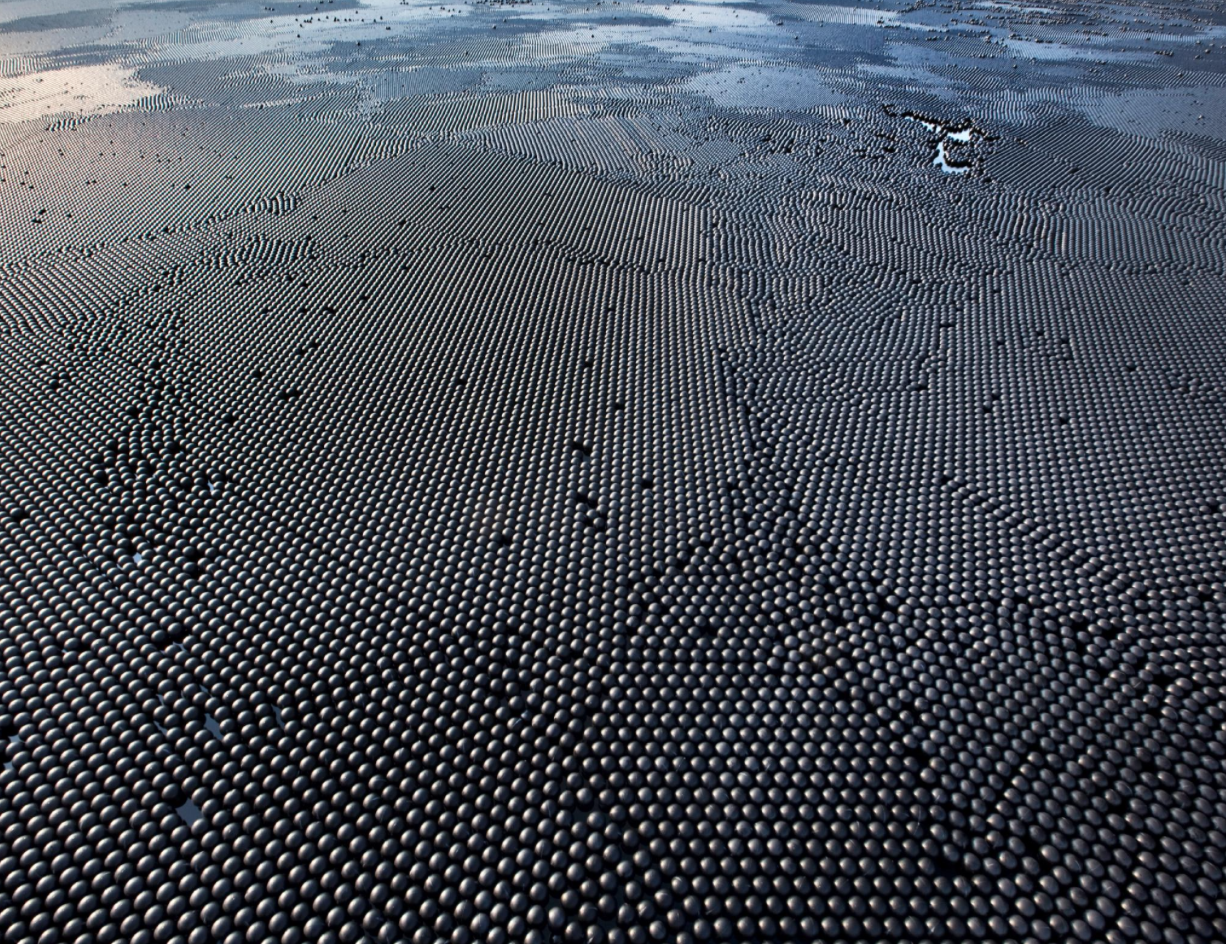
\includegraphics[width=0.75\linewidth,outer]{shade-balls}
  \caption[Shade balls floating on water: a 2d `crystal']{
    Shade balls covering the Los Angeles reservoir to cool water preventing evaporation and certain light-activated chemical reactions at the water surface.
    As macroscopic objects these balls interact as hard spheres, and they spontaneously form long-ranged orientational order seen as hexagonal domains.
    This is reminiscent of crystallisation in atomic systems.
    Image by Gerd Ludwig, \emph{National Geographic} (2007).}
  \label{fig:shade-balls}
\end{SCfigure}

Despite their coarse simplification of real atomic interactions, we see that hard spheres actually capture a lot of the essential physics.
To illustrate this consider the phase diagram of hard spheres Fig.\ \ref{fig:hs-phase-diagram}.
We see there is a freezing transition at $\eta = 0.494$, suggesting that the liquid will spontaneously order into a crystal at high densities.
This is surprising, in everyday scenarios (e.g.\ water) we are used to seeing crystallisation as one lowers temperature and the explanation normally given in classrooms is that the crystal is favoured due to attractions between molecules.
Now, in real systems crystallisation can also be triggered by changes to density also so density being a control parameter is not a problem, however the lack of attractions should, if this intuition were correct, prohibit crystallisation.

It turns out in the case of hard spheres that the crystal has a larger entropy above freezing, so entropy itself triggers crystallisation.
This was a hotly debated topic \cite{?,?,?} until is was solved by computer simulation in \cite{?,?,?} and experiment \cite{?,?,?}.
Part of the reason people could not believe that the crystal is entropically favoured, is because we often mistakenly take entropy to be a measure of disorder when it in fact more complicated.
The crystal might be more ordered than the liquid, with a lower \emph{configurational} entropy, however the entropy includes \emph{all} microstates not just averaged ones: the crystal is compensated by having a much larger \emph{vibrational} entropy than the liquid at high densities.
Including both these contributions leads to the phase diagram that we know today.

A similar effect is seen in balls floating on water as in e.g.\ peas in a saucepan or shade balls covering a reservoir.
The hard interactions between the balls causes%
\marginfootnote{In an attempt to find an everyday example, I have taken liberties with the interaction being purely hard; I suspect that floating balls feature effective attractions due to \emph{hydrodynamic} interactions at the water surface.}[-3cm]
them to `crystallise' at high densities as seen in Fig.\ \ref{fig:shade-balls}..
Strictly speaking these are not crystals in the sense of long-range \emph{translational} order, instead they are said to possess long-range \emph{orientational} order.
This subtlety emerges because the floating balls are confined to the water surface making them effectively two dimensional; fluctuations are strong enough in two dimensions to overcome truly long-ranged positional ordering \cite{MerminPRL1966,MerminPR1968}.

We have extolled the virtues of hard spheres, however this should not be interpretted as saying that this model system capture \emph{all} of the physics of real systems: it is a toy system after all.
They are merely a very good starting point for more complex systems.
As an example of physics they do \emph{not} capture, consider the critical point of real liquids.
Liquid-gas critical phenomena emerges from a competition between attractive and repulsive forces, with divergent fluctuations at the critical point.
It is thus impossible for a system with purely repulsive interactions, like hard spheres, to feature a critical point.
That being said, many theories predict critical phenomena quite well by taking a hard sphere potential and incorporating a mean-field like attractive perturbation \cite{?} so a hard sphere system provides a good reference point.

Hard spheres exist in more than just a theorist's imagination: they can be experimentally realised in colloidal experiments.
Colloidal suspensions are mixtures of solute immersed in a solvent composed of much smaller particles.
Colloidal particles are typically at the micron-scale.
These typically feature complex interactions \cite{Royall?,?,?} however these can be tailored to closely approximate hard sphere like interactions through steric stabilisation.
\todo{What is an aerosol? What is a dispersion?}
Colloidal experiments closely match hard simulations and theoretical predicitons \cite{?}.
Notably one can determine the phase diagram see Fig.\ \ref{fig:hs-phase-diagram}.
Note the glass at very high densities.

\begin{SCfigure}
  \missingfigure[figwidth=\linewidth]{}%
  \caption[The hard sphere phase diagram]{
    The hard sphere phase diagram, including the metastable branch.
    a: theoretical phase diagram.
    b: experiments, including the glass (image reproduced from \cite{?}).
    This is one of the most iconic images in the field, and no discussion of colloidal hard spheres would be complete without it.}
  \label{fig:hs-phase-diagram}
\end{SCfigure}

\begin{SCfigure}
  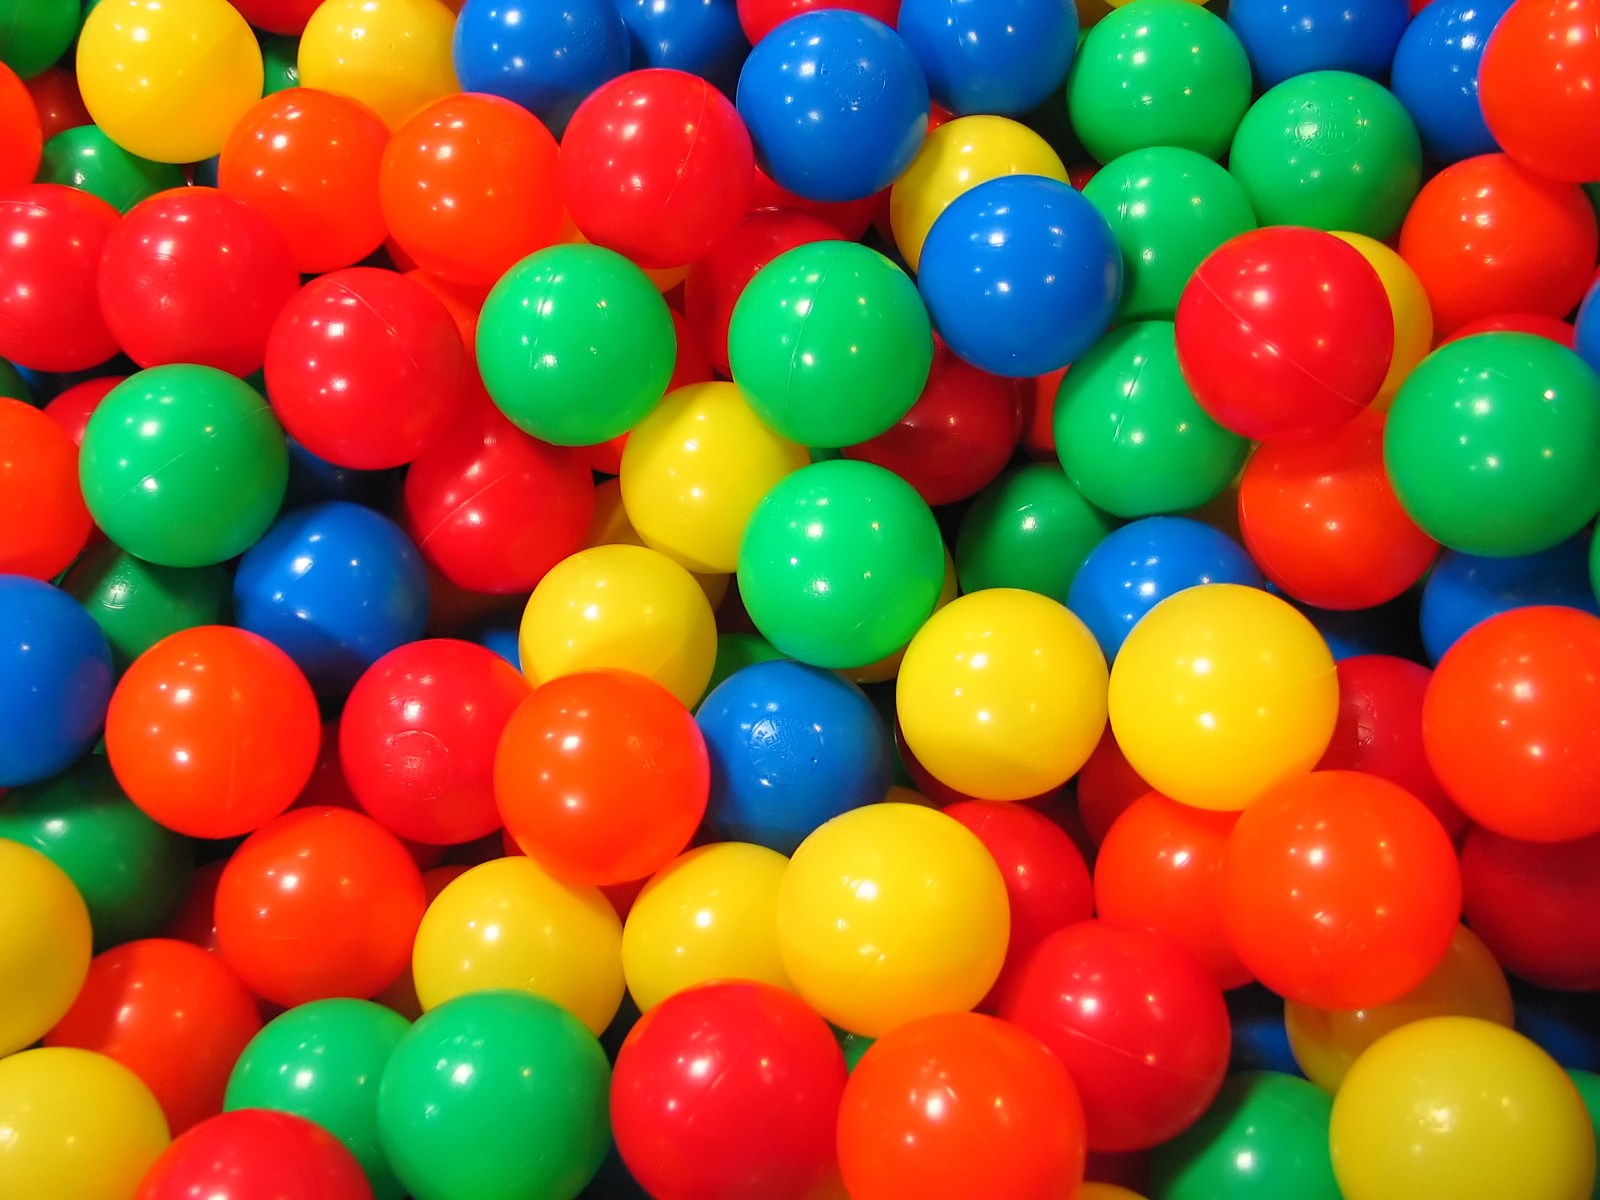
\includegraphics[width=0.75\linewidth,outer]{ball-pit-horizontal}
  \caption[Random close packing in a ball pit]{
    Random close packing of hard spheres in a ball bit.
    Image by Peter Ong.}
  \label{fig:rcp}
\end{SCfigure}

As the most widely studied model interaction potential we know a lot about its equilibrium structure (phase diagram) in bulk and even inhomogeneous thanks to density functional theory \cite{?,?,?}.
However, its behaviour off-equilibrium at high densities is hotly debated.
The two biggest unresolved research topics for this subject:
\begin{itemize}
\item \emph{Nucleation}: given that above freezing the crystal ? Theoretically predicted nucleation rates from simulation studies differ by 12 orders of magnitudes from experiments, purported to be the second biggest disagreement between theory and experiment in all of science \cite{?}.
\item \emph{Metastable liquid}: if one could avoid crystallisation and equilibrate only over the liquid microstates, what would be the ultimate fate of the liquid?
  We will talk more about this in \ref{?}.
\end{itemize}

There is a deep connection between hard spheres and computer science.
Packing problems have been studied \cite{Cohn,Conway,Sloane} and they are notoriously difficult; Kepler conjectured the optimal packing in 3d was the face-centred cubic/hexagonal close packing but it took 300(?check) years to solve this.
The final proof was computer aided, and not simple.
Packing problems are connected with encoding/encryption.
Transmitting a signal requires a way to encode a message across a band(?): if packed too tightly on the band(?) then noise will destroy the signal to it is desirable to optimise the sites for bits \cite{Cohn,?,?}.
Additionally, lattice based encryption techniques are one of the alternatives to prime factorisation: the coming development of quantum computers \cite{?,?} would render prime factorisation easy because of Shor's algorithm \cite{Shor?} rendering standard encryption techniques insecure.
The techniques developed for the mean field hard sphere problem have been applied to the perceptron model \cite{?}, and deep-learning neural networks which are naturally high dimensional problems lending themselves to a mean field treatment \cite{?}.

\begin{SCfigure}
  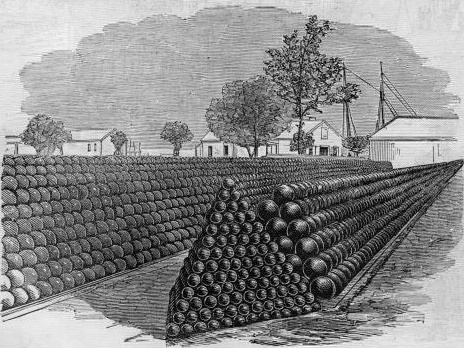
\includegraphics[width=0.75\linewidth,outer]{cannonballs}
  \caption[Close packed cannonballs]{
    Sketch of close-packed stacks of cannonballs in Fortress Monroe.
    Image by Stacy, \emph{Harper's weekly} (1861)}
  \label{fig:fcc}
\end{SCfigure}

Although hard spheres will be our focus, we will mention the importance of systems of hard particles of other shapes for self-assembly.
Self-assembly is an active area of soft matter: it is technologically desirable to tailor the final structure by controlling the building blocks.
Imagine assembling nanomachines or artificial cells by controlling the chemistry.
It is found that varying the size and shape of hard particles can reproduce all the complexity of the periodic table \cite{Glotzer?,Dijkstra?}.
Hard spheres are the simplest such system, so a theory which can treat other geometries is desirable.

The primary goal of this thesis is to advance the methods of treating liquids at high densities, particularly concerning the role of thermodynamics in dynamical arrest and nucleation.
These methods can be readily adapted to more complex systems, such as protein folding in aqueous solution or self-assembly of complex structures.

A secondary goal would be to advance the understanding of the fundamental theory of hard particles in some small way.
I have attempted to develop the geometrical theory behind the methods of Chapters \ref{?} and \ref{?} in a generally applicable way;
I have done this to the best of my ability, but my primary skills lie in numerical methods and I am a second-rate theoretician.

\section{Supercooled liquids and glasses}

It is widely reported that glass is actually liquid, and as evidence of this the thickness of old windows at the bottom is pointed to.
This is actually a matter of some dispute, but contains a grain of truth.
Pre-modern methods of creating window glass involved spinning molten glass on magma to flatten it out.
Centrifugal forces caused the glass to be thicker on the outer disk, so panes of glass would always be heavier in one direction%
\marginfootnote{And personally, if I were setting an uneven pane of glass I would place the heavy part at the bottom.}.

To a soft matter physicist glass is a broader term, referring to a wide class of materials while the window glass of common parlance is referred to by its chemical name \emph{silicate}.
This class of materials share many features of being disordered etc \cite{?} although in some sense they are connected by what they do \emph{not} do: which is flow on human timescales.
When I refer to `glass' I will be using it in this broad technical sense of a state of matter.
Some examples besides silicate:
\begin{itemize}
\item Most of the ice in the universe exists in an amorphous state in comets \cite{?}
\item Ceramics
\item Plastics: amorphous polymers
\end{itemize}
Of more abstract nature which could be called glassy though they are not materials
\begin{itemize}
\item Gels: super glasses, liquid like bit plus a network/backbone which has glassy dynamics
\item Neural networks
\item Non-deterministic polynomial time (NP) problems
\end{itemize}
We will not be directly addressing the latter type of more abstract problems which could be considered glasses, although they are arguably related due to a similar underlying disorder.
We will be focusing on only the most rudimentary of glassy phenomenology: the dynamical arrest of liquids at high densities/low temperatures when crystallisation is avoided.
Especially as it manifests in hard spheres, which as discussed is the reference system of choice for simple liquids.

So what do we mean by dynamical arrest.
Typically we can look at one of two (related) quantities: viscosity or relaxation time.
Viscosity measures how resistant the thing is to flow, while relaxation time measures the typical microscopic time for things to move around i.e.\ liquid like behaviour.
As a practical definition, a glass is defined in the lab as any material for which the relaxation time exceeds 100\ce{s}: this point is called the experimental glass transition.
This is somewhat arbitrary, although the location of the glass transition point is not particularly sensitive to where you set the threshold because of how rapidly the viscosity/times are increasing around there.
\todo{Need: Angell plot, fragile vs strong}

Personally, the observation that got me interested in the field is the entropy argument.
If one compares the difference between the entropy of the crystal and the glass, and extrapolates wildly one expects there to be a point where the glass has a lower entropy than the crystal.
This is not very meaningful by itself, as we have already established by discussing the crystal vibrational entropy can be quite subtle so it is possible for the liquid to have a lower vibrational entropy.
However, if one corrects this with more modern techniques to measure just the entropy corresponding to non-trivial motion we see that there is a point where the configurational (i.e.\ not purely vibrational) entropy vanishes: this would imply the system is frozen in a single configuration.
Such a point would define a transition to a genuine thermodynamic phase, an ideal glass.
\todo{Plots of configurational entropy}

A diverging timescale necessarily requires a diverging point-to-set length scale and a vanishing configurational entropy, a proof given in \cite{?}.
This must trivially occur at the very least $T=0\si{K}$ where relaxation timescales diverges, however much like the lack of a phase transition in the Ising model in $d=1$ this is not a true thermodynamic phase transition because it cannot be crossed.
Recent numerical evidence suggests that a model glassformer in $d=2$ does not show a transition, also vanishing at $T=0\si{K}$ \cite{Berthier?}.
So the central question of glass is what happens in $d=3$, is there a vanishing configurational entropy at a finite $T > 0$ with an accompanying thermodynamic glass transition?
In mean-field, formally in the limit of infinite spatial dimensions $d \to \infty$, the hard sphere system has been shown to have a true transition, however the critical dimensions are unknown so it is unclear what happens in $d=3$ \cite{Parisi,Zamboni,Charbonneau,Kurchan,?,?}.

\todo{Jamming: how does it relate to glass}

\section{Notes from Tarjus}

Overview of the glass transition.
Salient features: why hard, interesting, unique.

What is a glass?
Frozen in a (apparently) disordered state.
All sorts of glasses, structural, spin, orientational, electron, vortex.
Glasses formed by liquids, colloidal suspensions and polymers: traditional structural glasses.
Solid: doesn't flow on observational time, resists small/infinitesimal shear (acts like solid).
Amorphous, apparently amorphous: no periodic arrangement like in crystal.
Homogeneous makes useful for technology: useful for e.g.\ optical properties.

Hard glasses: high elastic constants.
Colloidal suspensions: soft matter version, small elastic constants.
Same phenomenology though.

Cooling a liquid.
Take thermodynamic quantity (e.g.\ volume, entropy, enthalpy): usually crystallise.
(Picture)
First-order transition bypassed by quick cooling.
Enter supercooled liquid phase.
No longer equilibrates/relax/flows, call it a glass: occurs at glass transition.
Glass is a solid for all practical purposes.

SC liquid: same characteristics as at equilibrium.
Independent of preparation: loses memory of initial preparation.
Measureable properties have time translational invariance/are stationary.
Time independence of all observables, i.e.\
\begin{equation}
  \langle A(t) \rangle = \langle A \rangle
\end{equation}
including correlation functions e.g.\
\begin{equation}
  \langle A(t) A(t') \rangle = \langle A(0) A(t - t') \rangle
\end{equation}
(equation for stationary)
Fluctuation-dissipation theorems.
Linear response regime: response to perturbation related to correlation function (spontaneous fluctuations).
\begin{equation}
  \chi_A (t, t')
  =
  - \beta \Theta(t - t')
  \frac{d}{dt}
  \left(
  \bigg\langle
  (A(t) - \langle A \rangle)
  (A(0) - \langle A \rangle)
  \bigg\rangle
  \right)
\end{equation}

\ifdefined\includebibliography
  \printbibliography
\fi
  
\end{document}

%TC: macro \marginfootnote [other]
%TC: envir SCfigure [] other
%TC: macrocount beginSCfigure [figure]
\documentclass[11pt,twoside]{report}
\usepackage{preamble}
\setcounter{chapter}{1}
\graphicspath{{../img/}}
\def\includebibliography{}

\externaldocument{morphometric-framework}

\begin{document}
\chapter{Background}
%\epigraph{It tells me that the Creator used the wrong kind of circles.}{Terry Pratchett, \emph{Pyramids} (1989).}
\epigraph{It was not certain what significance the ceremony held... but the formality was no less sacred for it being unintelligible}{Mervyn Peake, \emph{Titus Groan}, (1946).}

In this chapter we provide a \emph{concise} account of the foundational frameworks underlying the two themes of this thesis: \emph{integral geometry} and \emph{liquid state theory}.
I expect the reader to have a background in statistical physics, so my account of liquid state theory is not intended to be exhaustive; for more in-depth treatments see the references herein.
By contrast, I do \emph{not} expect much familiarity with integral geometry.
Understanding the underlying mathematical detail is not essential to follow the rest of the thesis, so I will focus more on the key concepts and notation than detailed derivation.
I anticipate the expert reader will skim over this chapter, so I have placed the important theorems in boxes as a guide to the most relevant parts.

As many-body correlation functions are a central theme of the results chapters, I have emphasised correlation functions in section \ref{sec:liquid-structure} on liquid structure to the point where I have somewhat belaboured giving the explicit forms and normalisations of the various correlation functions.
Even though we will only use one particular hierarchy of correlation functions in the results chapters, I personally found it helpful to have these formulas in one place.
I have found myself frequently revisiting the transformations between the various hierarchies of correlation functions, so I include them in anticipation that someone repeating or extending this work can profit from having a kind of ``cheat sheet''.

\input{integral-geometry}
\input{liquid-state-theory}
\input{density-functional-theory}
\input{supercooled-liquids}

\ifdefined\includebibliography
  \printbibliography
\fi

\end{document}

\documentclass[12pt]{report}
\usepackage{preamble}
\setcounter{chapter}{2}

\begin{document}
\chapter{Morphological framework for many-body correlations}
Mostly theoretical but with some numerical experiments which motivate/justify developments to the theory.
The main body of numerical work is left to the following chapter.

\section{Formalism for many-body correlations}

We write the $n$-particle distribution function $g^{(n)}$ as
\begin{equation}\label{eq:n-density-pdf}
  \textrm{Probability}\left( \textit{any } n \textrm{ particles in volume } d\vec{r}^n \right)
  \equiv
  \rho^n g^{(n)}(\vec{r}^n) \, d\vec{r}^n.
\end{equation}
In the main text, we expressed $g^{(n)}$ in terms of a generalised potential of mean force $\phi^{(n)}$: the reversible work required to insert $n$ particles into the liquid.
We decomposed $\phi^{(n)}$ into a local (potential energy) and solvent (free energy) component.
Although this quantity is quite intuitive and could be determined heuristically, here we give a short proof that this decomposition is formally exact and arises quite naturally from the definition of the distribution function.

In the grand-canonical ensemble the $n$-particle density $\rho^{(n)}(\vec{r}^n) \equiv \rho^n g^{(n)}$ is determined by integrating over the remaining degrees of freedom~\cite{Hansen2013}
\begin{equation}
  \rho^{(n)}(\vec{r}^n)
  = \frac{1}{\Xi} \sum_{N=n}^\infty \frac{z^N}{(N-n)!} \int e^{-\beta U_N} \, d\vec{r}^{(N-n)},
\end{equation}
where the activity is written in terms of the thermal de Broglie wavelength $\Lambda$ as $z = \exp{\beta\mu} / \Lambda^d$.
Changing the summation limits $N \rightarrow N+n$ we obtain
\begin{equation}\label{eq:n-density}
\begin{aligned}
  \rho^{(n)}(\vec{r}^n)
  &= \frac{z^n}{\Xi} \sum_{N=0}^\infty \frac{z^N}{N!} \int e^{-\beta U_{N+n}} \, d\vec{r}^{N} \\
 & = z^n e^{-\beta U_n} \left< e^{-\beta U_{n \leftrightarrow N}} \right>
\end{aligned}
\end{equation}
where in the latter step we decomposed the total potential $U_{N+n}$ into purely local and solvent terms, i.e.\ $U_{N+n} = U_n + U_N + U_{n \leftrightarrow N}$, where $U_\alpha$ for $\alpha \in \{n,N\}$ indicates the internal interactions between particles in component $\alpha$.
The ``interspecies'' interactions are contained within $U_{n \leftrightarrow N}$ which acts as an external field for the solvent.
The angled brackets indicate ensemble averaging over all arrangements of the solvent, i.e.\
\begin{equation}
  \left< \cdots \right> =
  \frac{1}{\Xi} \sum_{N=0}^\infty \frac{z^N}{N!} \int \left(\cdots\right) e^{-\beta U_N} \, d\vec{r}^N,
\end{equation}
with partition function of the unperturbed system $\Xi \equiv e^{-\beta \Omega_{hom}}$, where $\Omega_{hom} = -p V$ is the usual homogeneous grand potential.
Thus, \eqref{eq:n-density} becomes
\begin{equation}
  \rho^{(n)}(\vec{r}^n)
  = z^n e^{-\beta (U_n + \Omega - \Omega_{hom})}.
\end{equation}
where $\Omega$ is the grand potential of the solvent in the presence of the $n$-particle inhomogeneity.
Splitting the chemical potential into its ideal and excess parts so that $\beta\mu = \ln{\Lambda^d \rho} + \beta\mu^{ex}$ gives
\begin{equation}
  \rho^{(n)}(\vec{r}^n)
  = \rho^n e^{-\beta (U_n + \Omega - \Omega_{hom} - n\mu^{ex})}.
\end{equation}
The $n$-particle distribution functions are then determined from~\cite{Hansen2013}
\begin{equation}\label{eq:distribution-functions}
  g^{(n)}(\vec{r}^n)
  \equiv \frac{\rho^{(n)}(\vec{r}^n)}{\rho^n}
  = e^{-\beta(U_n + \Delta\Omega - n\mu^{ex})}
\end{equation}
where $\Delta\Omega = \Omega - \Omega_{hom}$ giving the generalised potential of mean force stated in the main text.

The above is essentially the generalisation of the \emph{potential distribution theorem} \cite{Widom1963,Widom1982} to many-particles. See Ref.\ \cite{Rowlinson2002} and references therein for a detailed review of this approach.

\section{Morphological form of the potential of mean force}
Justification of assumptions: additivity, continuity and motion invariance
\subsection{Limitations known from DFT literature}
\subsection{As a generalisation of scaled particle theory}
And the limitations this implies.

\section{Worked examples where morphometric form can be exact}
Under certain conditions.
\subsection{Low density limit in arbitrary dimensions from lowest order terms in the virial expansion of the pressure}
\subsection{Arbitrary densities at large lengthscales}
\subsection{Hard rods (dimension d = 1) at all densities}
\subsubsection{Exact result from DFT}
\subsubsection{Morphometric result}
Explore where additivity, continuity and motion invariance apply.
\subsubsection{Implications for higher dimensions}

\section{Derivation of thermodynamic coefficients for hard spheres in $d = 3$}

\subsubsection{Scaled particle route}

We describe here in more detail the derivation of the first set of morphometric coefficients, equivalent to those given in \cite{Hansen-Goos2006} through fundamental measure theory (FMT).
The derivation sketched below avoids use of FMT, instead favouring a geometric formulation equivalent to the scaled particle approach of Reiss \emph{et al}.\ \cite{Reiss1959,Reiss1960}.
The standard scaled particle approach considers an expansion of the grand potential surrounding a spherical solute in powers of radii; here, we modify the \emph{ansatz} to use morphological measures instead, so that the resulting theory is more naturally extended to geometries of arbitrary shapes.
Additionally, we impose the Carnahan-Starling equation of state as an \emph{input} whereas the Percus-Yevick equation of state is an \textit{output} of standard scaled particle approaches.

Following the protocol of scaled particle theories, we consider the insertion of a hard ball of radius $R-\frac{\sigma}{2}$ into the liquid at the origin.
This choice of radius ensures that contact with the \emph{center} of solvent particles occurs at distance $R$ from the point of insertion i.e.\ $\rho(r) = 0$ for $r < R$.
Writing the change in the grand potential due to the insertion of the ball in its morphometric form (from \eqref{eq:surface-tension} and \eqref{eq:morphometric-surface-tension} of the main text), we have the \emph{ansatz}
\begin{equation}\label{eq:morph-ball-solvation}
  \Delta \Omega(R) =
  \frac{4\pi R^3}{3} p +
  4\pi R^2 \, \gamma_\infty +
  4\pi R \, \kappa +
  4 \pi \, \overline{\kappa}.
\end{equation}
If an equation of state for the pressure is taken as input, only three equations are needed to set the remaining coefficients of surface tension $\gamma_\infty, \kappa$ and $\overline{\kappa}$.

Restating the expressions for the insertion of a hard point and a new particle from the main text as
\begin{align}
  \label{eq:spt-point} \Delta\Omega(R=0) &= -k_B T \ln{(1- \eta)}, \\
  \label{eq:spt-mu} \Delta\Omega\left(R=\frac{\sigma}{2}\right) &= \mu^{ex},
\end{align}
we need one more equation to set the thermodynamic coefficients for the theory.
Following Ref.\ \cite{Bryk2003} we take the normal derivative of $\Omega$ with respect to $R$, and noting that $\Delta\Omega(R) = \Omega(R) - \Omega_{hom}$ gives
\begin{equation}\label{eq:spt-derivative}
  \left( \frac{\partial \Delta \Omega}{\partial R} \right)_{\mu,V,T} =
  \left( \frac{\partial \Omega}{\partial R} \right)_{\mu,V,T} =
  \int
  \frac{\delta \Omega[\rho_0(\vec{r})]}{\delta \rho}
  \left( \frac{\partial \rho_0(\vec{r})}{\partial R} \right)_{\mu,V,T}
  \, d\vec{r} +
  \int
  \rho_0(\vec{r})
  \left( \frac{\partial \phi_{ext}(\vec{r})}{\partial R} \right)_{\mu,V,T}
  \, d\vec{r},
\end{equation}
where $\rho_0$ is the equilibrium density profile and $\phi_{ext}$ is the external potential (i.e.\ the potential of the ball).
In equilibrium $\Omega$ is minimised so
\begin{equation}
  \left.
  \frac{\delta \Omega[\rho(\vec{r}); \phi_{ext}]}{\delta \rho}
  \right|_{\rho(\vec{r})=\rho_0(\vec{r})} = 0,
\end{equation}
so the first integral in \eqref{eq:spt-derivative} vanishes.
As the ball is hard, the external potential and its derivative are zero everywhere except at the surface $R$ where both $\rho_0$ and $\phi_{ext}$ are discontinuous.
We consider its Boltzmann weight, i.e.\
\begin{equation}
  e^{-\beta\phi_{ext}(\vec{r})} = \Theta(|\vec{r}| - R).
\end{equation}
Taking the derivative of both sides gives
\begin{equation}
  \beta\left( \frac{\partial\phi_{ext}(\vec{r})}{\partial R} \right)_{\mu,V,T} =
  \delta(|\vec{r}| - R) e^{\beta\phi_{ext}(\vec{r})}
\end{equation}
Inserting this expression into \eqref{eq:spt-derivative} and using the fact that $\rho(\vec{r}) e^{\beta\phi_{ext}(\vec{r})}$ is continuous (c.f.\ Ref.\ \cite{Hansen2013}) gives the contact theorem
\begin{equation}
  \beta \left( \frac{\partial \Omega}{\partial R} \right)_{\mu,V,T} =
  4\pi R^2 \rho(R).
\end{equation}
When $R = \sigma$ the inserted ball is equivalent to the hard sphere particles themselves, so $\Omega = \mu^{ex}$ and the contact density is $\rho(\sigma) = \rho \, g^{(2)}(\sigma)$ giving
\begin{equation}\label{eq:spt-contact-density}
  \left. \beta \left( \frac{\partial \Delta \Omega}{\partial R} \right)_{\mu,V,T}
  \right|_{R = \sigma}
  =
  \left. \beta \left( \frac{\partial \Omega}{\partial R} \right)_{\mu,V,T}
  \right|_{R = \sigma}
  =
  %\beta \frac{\partial \mu^{ex}}{\partial \sigma} =
  4\pi \sigma^2 \rho \, g^{(2)}(\sigma),
\end{equation}
or written in morphometric form using \eqref{eq:morph-ball-solvation} we have
\begin{equation}
  4\pi \sigma^2 \, p +
  8\pi \sigma \, \gamma_\infty +
  4\pi \, \kappa =
  \frac{4\pi \sigma^2 \rho}{\beta} \, g^{(2)}(\sigma).
\end{equation}
Applying the virial theorem (equation \eqref{eq:contact-g} in the main text) to the right hand side gives the final expression:
\begin{equation}\label{eq:spt-virial}
  4\pi \sigma^2 \, p +
  8\pi \sigma \, \gamma_\infty +
  4\pi \, \kappa =
  \frac{6}{\beta\sigma} \left( \frac{\beta p}{\rho} - 1 \right).
\end{equation}
Together \eqref{eq:spt-point}, \eqref{eq:spt-mu} and \eqref{eq:spt-virial} form a complete system of equations which we solve to obtain the coefficients
\begin{subequations}
  \begin{align}
    \frac{\beta \gamma_\infty^{WBII}}{R \rho} &=
    \left(\frac{\pi}{6\eta^2} - \frac{5\pi}{18\eta}\right) p -
    \frac{\mu^{ex}[p]}{3\eta} -
    \frac{\ln{(1-\eta)}}{3\eta} -
    \frac{1}{\eta}
    \label{eq:spt-gamma}
    \\
    \frac{\beta \kappa^{WBII}}{R^2\rho} &=
    \left( \frac{4\pi}{9\eta} - \frac{\pi}{2\eta^2} \right) p +
    \frac{4\mu^{ex}[p]}{3\eta} + \frac{4\ln{(1-\eta)}}{3\eta} + \frac{3}{\eta}
    \\
    \frac{\beta \overline{\kappa}^{WBII}}{R^3\rho} &=
    \left( \frac{\pi}{3\eta^2} - \frac{2\pi}{9\eta} \right) p -
    \frac{\mu^{ex}[p]}{\eta} - \frac{4\ln{(1-\eta)}}{3\eta} - \frac{2}{\eta}.
  \end{align}
\end{subequations}
Inserting the Carnahan-Starling parameters \eqref{eq:cs-pressure} and \eqref{eq:cs-mu} gives the coefficients explicitly as
\begin{subequations}
  \begin{align}
    \frac{\beta p^{WBII}}{\rho} &=
    \frac{1 + \eta + \eta^2 - \eta^3}{(1-\eta)^3}
    \\
    \frac{\beta \gamma_\infty^{WBII}}{R\rho} &=
    -\frac{1 + 2\eta + 8\eta^2 - 5\eta^3}{3(1-\eta)^3}
    - \frac{\ln{(1-\eta)}}{3\eta}
    \\
    \frac{\beta \kappa^{WBII}}{R^2\rho} &=
    \frac{4 - 10\eta + 20\eta^2 - 8\eta^3}{3(1-\eta)^3} + \frac{4 \ln{(1-\eta)}}{3\eta}
    \\
    \frac{\beta \overline{\kappa}^{WBII}}{R^3\rho} &=
    - \frac{4 - 11\eta + 13\eta^2 - 4\eta^3}{3(1-\eta)^3} - \frac{4 \ln{(1-\eta)}}{3\eta},
  \end{align}
\end{subequations}
which are \emph{identical} to the coefficients derived from the WBII free energy functional in Ref.\ \cite{Hansen-Goos2006}.
Remarkably, we have obtained these coefficients through a route completely different from their original derivation.
In Ref.\ \cite{Hansen-Goos2006} the coefficients were determined within FMT by taking the limit of a binary mixture where one component is infinitely dilute.
Here we completely avoided FMT, in favour of geometrical arguments similar to standard scaled particle approaches.
This suggests that the above scaled particle argument is somehow built into the structure of the WBII functional; we note that this is a nonobvious fact which cannot be determined from the form of the functional alone, nor is it obvious how it emerges from its original derivation.

Finally, note that (as described in the main text) the resulting $g^{(2)}$ performs poorly in the supercooled regime as compared with the ``exact'' result from virial theorem i.e.\ Eq.\ \eqref{eq:contact-g} in the main text.
In Fig.\ \ref{fig:contact-g} we plot the contact value with this set of coefficients, finding that it is reasonably accurate until around the freezing density where contact correlations spuriously decay.
The next section will detail how to modify the derivation to produce coefficients which describe more accurate correlation functions at high densities.

\subsection{Aside: scaled particle theory extension for dimers}

I was unaware of work by Stillinger et al \cite{Stillinger2006} before publishing on the morphometric approach, but upon discovering this work I realised their ideas are very similar in nature.
Here I present similar results but using the morphometric notation.%
\marginfootnote{The purpose of this section needs to be fleshed out and made \emph{very} clear, otherwise the reader will get lost quickly.
  This section \emph{is} important as we explore the boundaries of where the morphometric approach can fail: this is a great testbed for continuity, and allows us to argue the accuracy of the approach applied to local structures.}

We have the probability of any number of particles existing inside the cavity
\begin{equation}
  \sum_{n=0}^\infty p_n (\lambda) = 1
\end{equation}
Giving the probability the cavity is empty due to a spontaneous thermal fluctuation
as
\begin{equation}
  p_0 (\lambda) = e^{-\beta W(\lambda)}
  = 1 - \sum_{n=1}^\infty p_n (\lambda).
\end{equation}
The singular nature of the hard sphere interaction ensures there is a maximum number of particles that can fit inside any finite sized cavity (the optimal packing), so we define
\begin{equation}
  n^*(\lambda) = \max{n(\lambda)},
\end{equation}
and thus
\begin{equation}
  p_0 (\lambda) = e^{-\beta W(\lambda)}
  = 1 - \sum_{n=1}^{n^*(\lambda)} p_n (\lambda).
\end{equation}

Following Stillinger we generalise to two cavities.
Define work to insert both cavities as $W^{(2)}(r,\lambda)$.
We then have the generalisaton
\begin{equation}
  p_0^{(2)} (\lambda) = e^{-\beta W^{(2)}(\lambda)}
  = 1 - \sum_{n=1}^{\max{n^{(2)}(\lambda)}} p_n^{(2)} (\lambda).
\end{equation}
We have the conditions:%
\marginfootnote{To do: Make this notation more consistent and able to handle different numbers of cavities. We don't want to just recycle Stillinger's notation: we want to be consistent with the rest of the thesis.}
\marginfootnote{Also, need to define $\lambda$ as the cavity diameter}[4cm]
\begin{align}
  \lim_{r \to 0} W^{(2)}(r; \lambda) &= W^{(1)}(\lambda) \\
  \max{n^{(2)}(r; \lambda)} &= 1
  \quad \forall \; r + 2\lambda < 1 \\
  \lim_{r \to \infty} W^{(2)}(r; \lambda) &= 2 W^{(1)}(\lambda) \\
  \max{n^{(2)}(r; \lambda)} &\le 2 \max{n^{(1)}(\lambda)}
  \quad \forall \; r > 2\lambda
\end{align}
Which gives us the `point' insertion condition (where $\max{n^{(2)}(r; \lambda)} = 1$)
\begin{equation}
  \beta W^{(2)}(r; \lambda) = -\ln (1 - \rho V(r; \lambda))
\end{equation}

Hausdorff distance is simply $r$, so how the hell is the Euler characteristic of their union continuous with respect to $r$? It is discontinuous at $r = 2\lambda$.

\subsubsection{Virial route}

In this section we give the detailed steps used in the derivation of the new set of morphometric coefficients, following the direction laid out in the main text.
In section \ref{SI:two-particles} above the morphological form of $g^{(2)}$ was computed explicitly; this derivation imposes the contact density using $\rho(\sigma) = \rho \, g^{(2)}(\sigma)$ with this explicit form.

From \eqref{eq:g2-explicit} the potential of mean force for neighbouring particles reduces to $\phi^{(2)}(r) = \Delta\Omega(r) - 2\mu^{ex}$ if they do not overlap, giving
\begin{equation}
  \begin{split}
  \phi^{(2)}(r) &\equiv - k_B T \ln g^{(2)}(r) \\
  &= pV(r) + \gamma_\infty A(r) + \kappa C(r) + \overline{\kappa} X(r) - 2\mu^{ex}
  \quad \forall \; \sigma \le r \le 2\sigma.
  \end{split}
\end{equation}
Inserting the morphological quantities at contact from \eqref{eq:g2-explicit-morph} gives
\begin{equation}
  \phi^{(2)}(\sigma) =
  \frac{9\pi \sigma^3}{4} p +
  6\pi\sigma^2 \, \gamma_\infty +
  \left( 6\pi\sigma - \frac{\pi^2\sigma}{2\sqrt{3}} \right) \, \kappa +
  4\pi \, \overline{\kappa}
  - 2\mu^{ex}[p].
\end{equation}
Equating this with $-k_B T \ln g^{(2)}(\sigma)$ and using the virial theorem (Eq.\ \eqref{eq:contact-g} in the main text) gives the final expression
\begin{equation}\label{eq:v-virial}
  \frac{9\pi \sigma^3}{4} p +
  6\pi\sigma^2 \, \gamma_\infty +
  \left( 6\pi\sigma - \frac{\pi^2\sigma}{2\sqrt{3}} \right) \, \kappa +
  4\pi \, \overline{\kappa} = 
  2\mu^{ex}[p] - \beta^{-1} \ln{\frac{3}{2\pi \rho \sigma^3} \left( \frac{\beta p}{\rho} - 1 \right)}.
\end{equation}
We will use this last expression instead of the contact theorem \eqref{eq:spt-virial} in order to obtain new coefficients.
Together \eqref{eq:spt-point}, \eqref{eq:spt-mu} and \eqref{eq:v-virial} solve to give coefficients:
\begin{subequations}
  \begin{align}
    \frac{\beta \gamma_\infty^{V}}{R\rho} &=
    \frac{ (18\pi - 7\sqrt{3} \pi^2) p + 6\sqrt{3}\pi \mu^{ex}[p]
      - 6(12 - \sqrt{3}\pi) \ln{(1-\eta)}
      - 72\ln{\left( \frac{\pi p - 6\eta}{24\eta^2} \right)} }
    {54(\sqrt{3}\pi - 4) \eta}
    \label{eq:virial-gamma}
    \\
    \frac{\beta \kappa^{V}}{R^2\rho} &=
    \frac{ 5\pi p - 12 \mu^{ex}[p] + 24 \ln{(1-\eta)}
      + 36\ln{\left( \frac{\pi p - 6\eta}{24\eta^2} \right)} }
    {9(\sqrt{3}\pi - 4) \eta}
    \\
    \frac{\beta \overline{\kappa}^{V}}{R^3\rho} &=
    - \frac{
      (18\pi - 2\sqrt{3} \pi^2) p - (36 - 3\sqrt{3}\pi) \mu^{ex}[p] + 12\sqrt{3}\pi \ln{(1-\eta)}
      + 72\ln{\left( \frac{\pi p - 6\eta}{24\eta^2} \right)} }
    {27(\sqrt{3}\pi - 4) \eta},
  \end{align}
\end{subequations}
which upon insertion of the Carnahan-Starling parameters \eqref{eq:cs-pressure} and \eqref{eq:cs-mu} gives the coefficients explicitly as
\begin{subequations}
  \begin{align}
    \frac{\beta p^{V}}{\rho} &=
    \frac{1 + \eta + \eta^2 - \eta^3}{(1-\eta)^3} \\
    \frac{\beta \gamma_\infty^{V}}{R\rho} &=
    \frac{ 18\eta \frac{1 + \eta + \eta^2 - \eta^3}{(1-\eta)^3}
      + \sqrt{3}\pi\eta \frac{1 - 16\eta - 4\eta^2 + 7\eta^3}{(1-\eta)^3}
      - (12 - \sqrt{3}\pi) \ln{(1-\eta)}
      - 12\ln{\left( \frac{2 - \eta}{2(1-\eta)^3} \right)} }
    {9(\sqrt{3}\pi - 4) \eta} \\
    \frac{\beta \kappa^{V}}{R^2\rho} &= -
    \frac{ 2\eta \frac{11 - 23\eta + \eta^2 + 5\eta^3}{(1-\eta)^3}
      - 8 \ln{(1-\eta)}
      - 12\ln{\left( \frac{2 - \eta}{2(1-\eta)^3} \right)} }
    {3(\sqrt{3}\pi - 4) \eta} \\
    \frac{\beta \overline{\kappa}^{V}}{R^3\rho} &=
    \frac{ 12\eta \frac{5 - 12\eta + 3\eta^3}{(1-\eta)^3}
      - \sqrt{3}\pi\eta \frac{4 - 13\eta - \eta^2 + 4\eta^3}{(1-\eta)^3}
      - 4\sqrt{3}\pi \ln{(1-\eta)}
      - 24\ln{\left( \frac{2 - \eta}{2(1-\eta)^3} \right)} }
    {9(\sqrt{3}\pi - 4) \eta}.
  \end{align}
\end{subequations}
Unlike the WBII coefficients above these are entirely new, and produce significantly more accurate correlation functions at high densities as described in the main text.
The pair correlation produced by these coefficients (black line in Fig.\ \ref{fig:contact-g}) is self-consistent with CS at contact by construction, but as an additional bonus we find that the new coefficients provide a theory that outperforms the older WBII approach across the whole range of distances typical of neighbouring particles (inset of Fig.\ \ref{fig:contact-g}).
The latter observation enables us to accurately model complex many-particle local structures.

However, it should be noted that the planar surface tension $\gamma_\infty^{V}$ is considerably less accurate than $\gamma_\infty^{WBII}$ as compared with molecular dynamics studies in \cite{Davidchack2016}.
For this reason, WBII coefficients may give more accurate grand potentials (and thus correlations) for large solutes where the surface becomes approximately planar.

\section{Accuracy of predicted distribution functions in $d = 3$}
\subsection{Comparison with molecular dynamics simulations}
\subsection{Comparison with Kirkwood superposition approximation}

\end{document}

%TC: macro \marginfootnote [other]
%TC: envir SCfigure [] other
%TC: macrocount beginSCfigure [figure]
\documentclass[11pt,twoside]{report}
\usepackage{preamble}
\setcounter{chapter}{4}
\graphicspath{{../img/}}
\def\includebibliography{}

\externaldocument{background}
\externaldocument{supercooled-liquids}
\externaldocument{morphometric-framework}
\externaldocument{appendix-full-geometry}
\externaldocument{appendix-bayesian}

\begin{document}
\chapter{Local structure in the hard sphere liquid}
\epigraph{\textbf{hardball 1.1} \emph{informal} Uncompromising and ruthless methods or dealings.}{Oxford English Dictionary (2019).}
\label{chapter:morphometric-applications}

This chapter applies the theory developed in the previous chapter to the treatment of local structures in the hard sphere liquid.
Using the framework of many-body correlations and the morphometric approach, we calculate absolute free energies of local geometric motifs.
We find these to be in excellent quantitative agreement with molecular dynamics simulations across the liquid and supercooled liquid regimes.
We find a bimodality in the density library of states where fivefold symmetric structures appear lower in free energy than fourfold symmetric structures, and from a single reaction path predict an Arrhenius-like scaling of local relaxation dynamics.
The method provides a new route to assess changes in the free energy landscape at volume fractions dynamically inaccessible to conventional techniques.

The majority of this chapter contains work published as Ref.\ \cite{RobinsonPRL2019}.
Towards the end of this chapter we introduce an unpublished method using Bayesian inference to evaluate the free energy of local structures in hard spheres, which has the potential to treat the saddles of the hard sphere energy landscape.

%% While `sphere' and `ball' are used interchangeably in physics (and colloquially), in geometry they refer to different things: balls $\ball^d$ are the solid objects whereas spheres are the boundaries $\partial \ball^d$.
%% As such, physicists really mean `hard balls' rather than hard spheres; the epigraph rang true for me as I undertook the work of this chapter.

\section{Introduction}

While mean-field theories provide insight into complex phenomena, physical accuracy is ensured only by a proper treatment of correlations.
For example, the simplest case of two-body correlations is at the foundation of predictive theories of the liquid state (section \ref{sec:liquid-state-theory}), colloids, and complex plasmas \cite{LikosPR2001,Ivlev2012}.
%, and some forms of active matter \cite{Bechinger2016}.
In particular, the thermodynamics of simple liquids with solely pairwise interactions can be exactly expressed in terms of two-body correlations (section \ref{sec:thermodynamic-routes}).
However, to resolve these integrated quantities \emph{spatially} into structural motifs, and \emph{temporally} into specific dynamical events, one needs to calculate many-body correlations.
While such a many-body approach may often be neglected in normal liquids, long-standing challenges such as the dramatic dynamical changes occurring in supercooled liquids approaching their glass transition \cite{BerthierRMP2011,RoyallPR2015} and phase transitions such as crystal nucleation \cite{RussoSR2012} call for a many-body description.

In the case of supercooled liquids, theories based on pair correlations such as the standard mode-coupling framework \cite{Gotze2009} fail to account for activated events thus predicting a spurious ergodicity breaking transition \cite{BrambillaPRL2009,HallettNC2018}.
Activated dynamics are often rationalised through collective (i.e.\ many-body) effects within contrasting thermodynamic and purely dynamic scenarios \cite{LubchenkoARPC2007,TarjusJPCM2005,BiroliPRL2006,JanssenPRL2015,SzamelPTEP2013,ChandlerARPC2010}.
These include exact mean-field results in high dimensions \cite{ParisiRMP2010,CharbonneauARCMP2017} whose relevance in finite-dimensional systems is hotly debated \cite{WyartPRL2017}.
A finite-dimensional theoretical description of many-body effects is therefore much needed.
We discussed the various theories mentioned above in more detail in chapter \ref{chapter:glass}.

However, many-body correlations are challenging to compute and typically combine both energetic and entropic contributions.
Physical insight can be gleaned by exploring the potential energy landscape of isolated clusters \cite{Wales2004,ArkusPRL2009}, but such methods are only exhaustive for small system sizes.
This limitation has been partly addressed by embedding clusters in a mean-field approximation of the surrounding liquid \cite{MossaJCP2003,MossaJNS2006}.
Nonetheless, this approach neglects by construction the intra-cluster entropic contributions that may dominate in the supercooled regime of interest.
Furthermore, computer simulations, which naturally deliver full many-body correlations are limited in the range of dynamics they can access, hampering an approach to the glass transition, except for recent developments with certain models \cite{BerthierPRL2016}.

In this chapter we place theoretical predictions of many-body local structure on a fundamentally more rigorous footing using inhomogeneous liquid state theory \cite{EvansAP1979}, which we reviewed in section \ref{sec:dft} and advanced in chapter \ref{chapter:morphometric-framework}.
Using the morphometric approach to treat the many-body interactions between a local subsystem and the remaining liquid, we can directly access the many-body \textit{free} energy of local arrangements of particles.
This allows us to predict the populations of specific local structures in the bulk system across the entire liquid phase and beyond the dynamically accessible supercooled regime.

\section{Free energy of local structures}

%\subsection{Concentrations of local structure}

%% How do we define a local structure?
%% Most of the literature on structure in amorphous systems falls into one of either two categories
%% Almost all methods for Common methods:
%% \begin{itemize}
%%   \item Bond orientational order parameters
%%   \item Bond networks: take some bond detection algorithm (voronoi,
%% Fom the partition function of the potential of mean force
%% Suppose we have a definition of a
%% \end{itemize}

From the definition of the probability density function  \eqref{eq:n-particle-density-pdf} defining the $n$-particle density, the total number of a local structure in a system volume $V$ is
\begin{equation}\label{eq:structure-population}
  \mathcal{N}
  =
  \frac{1}{n!}
  \int_{\mathcal{Q}}
  \rho^n g^{(n)}(\vec{r}^n)
  \, d\vec{r}^n,
\end{equation}
where $\mathcal{Q}$ is the domain \emph{defining} the particular local structure.
In terms of the potential of mean force \eqref{eq:potential-mean-force} this would be written equivalently as
\begin{equation*}
  \mathcal{N}
  =
  \frac{1}{n!}
  \int_{\mathcal{Q}}
  \rho^n \exp{\left(-\beta\phi^{(n)}(\vec{r}^n)\right)}
  %e^{-\beta \phi^{(n)}(\vec{r}^n)}
  \, d\vec{r}^n,
\end{equation*}
which has a similar structure as the canonical partition function \eqref{eq:canonical-partition} so we can think of structure population $\mathcal{N}$ as being the equivalent partition function in our ensemble%
\marginfootnote{Formally, this is the \emph{semi-grand canonical ensemble} because there is a chemical potential $\mu$ for the bulk component, but also a fixed number of particles for the local component $n$.}.
From the latter observation we could define a free energy for the local structure from $-k_B T \, \ln{\mathcal{N}}$,
%% \begin{equation*}
%%   \beta F = - \ln{\mathcal{N}},
%% \end{equation*}
but we will find it more useful to define the free energy as an excess quantity.
Specifically, we exploit translational invariance of $\phi^{(n)}$ in the uniform liquid to integrate the center of mass over the system volume, as in
\begin{equation}
  \mathcal{N}
  =
  \frac{\rho^n V}{n!}
  \int_\mathcal{D}
  g^{(n)}(\vec{r}^{n-1})
  \, d\vec{r}^{n-1},
\end{equation}
defining the internal structure space $\mathcal{D}$ through $\mathcal{Q} = \mathcal{D} \times V^d$.
The prefactor $\rho^n V$ is the trivial scaling of the ideal gas, so we define the free energy of the structure through the excess quantity%
\marginfootnote{Note: in previous chapters we used the symbol $F$ to refer to the Helmholtz free energy; here it will \emph{only} refer to the free energy of a local structure.}
\begin{equation*}
  e^{-\beta F}
  =
  \frac{\mathcal{N}}{\sigma^{d(n-1)} \rho^n V},
\end{equation*}
with powers of particle diameter $\sigma$ introduced to make the right-hand side dimensionless.
Note that $\mathcal{N} / V$ is the \emph{concentration} of the structure, so the right-hand side could be thought of as an excess concentration.
Written explicitly, the free energy of the local structure is
\begin{equation}\label{eq:local-structure-free-energy}
  \begin{split}
    \beta F
    &=
    -\ln{
      \left(
        \frac{1}{\sigma^{d(n-1)} n!}
        \int_{\mathcal{D}}
        g^{(n)}(\vec{r}^{n-1}) \, d\vec{r}^{n-1}
      \right)
    },
    \\
    &=
    -\ln{
      \left(
        \frac{1}{\sigma^{d(n-1)} n!}
        \int_{\mathcal{D}}
        \exp{\left(-\beta\phi^{(n)}(\vec{r}^{n-1})\right)}
        \, d\vec{r}^{n-1}
      \right)
    }.
  \end{split}
\end{equation}
Evaluating this free energy thus requires a closure for $\phi^{(n)}$, a definition of the structure to set integration limits through $\mathcal{D}$, and a method of actually doing the integration.

We calculate $\phi^{(n)}$ from its definition \eqref{eq:potential-mean-force} and using the morphometric \emph{ansatz} \eqref{eq:morph-ansatz} as a closure for $\Delta \Omega$.
Our focus is on $d=3$, so we use the virial route coefficients \eqref{eq:virial-coefficients} with the Carnahan-Starling equation of state \eqref{eq:cs-pressure} because of the accuracy of the resulting correlation functions (cf.\ section \ref{sec:framework-numerics}).
We have already seen how this equation of state is accurate at high densities (Fig.\ \ref{fig:swap-eos}), though it is worth emphasising that it must fail at some point setting limits on our approach.
%The pair correlation produced by these coefficients is self-consistent with CS at contact by construction; moreover, the new coefficients provide a theory that outperforms the older WBII approach across the whole range of distances typical of neighbouring particles (SM).
%This enables us to accurately model complex many-particle local structures.
We calculate the morphological quantities $\{V, A, C, X\}$ using an algorithm described in Ref.\ \cite{KleninJCC2011}, which we have extended to calculate curvature measures (see details in Appendix \ref{appendix:computational-geometry}).

In conventional energy landscape approaches, a structure%
\marginfootnote{Energy landscape approaches are actually more general than just pertaining to local structures, as they could in principle refer to the landscape of a macroscopic system as they do in e.g.\ mean field approaches (cf.\ section \ref{sec:mean-field-glass}).
  It is only in this context of small system sizes that they refer to local structures.}
would be defined by the region, or \emph{basin}, surrounding an energy minimum called the \emph{inherent state} \cite{StillingerPRA1982,StillingerS1995,Wales2004}.
Defining the location of the inherent state as
\begin{equation*}
  \vec{x}^*
  :=
  \argmin_{\vec{x} \in \mathcal{D}}{\left( \phi^{(n)}(\vec{x}) \right)},
\end{equation*}
with $\vec{x}$ as shorthand for $\vec{r}^{n-1}$.
The partition function would then be evaluated using via a perturbation theory around the inherent state i.e.\ from the Taylor expansion \cite{Wales2004}
\begin{equation*}
  \phi^{(n)}(\vec{x})
  =
  \phi^{(n)}(\vec{x}^*)
  + \frac{1}{2} (\vec{x} - \vec{x}^*) \cdot
  \vec{\nabla}\vec{\nabla} \phi^{(n)}(\vec{x}^*)
  \cdot (\vec{x} - \vec{x}^*)
  + \mathcal{O}(\vec{x}^3)
\end{equation*}
which is valid in the case of \emph{smooth} potentials where $\vec{\nabla} \phi^{(n)}(\vec{x}^*) = 0$.
Then, \cite{Wales2004}
\begin{equation}\label{eq:harmonic-approximation}
  \begin{split}
    \int_\mathcal{D} e^{-\beta\phi^{(n)}(\vec{x})} d\vec{x}
    &\simeq
    e^{-\beta\phi^{(n)}(\vec{x}^*)}
    \int_\mathcal{D}
    \exp{\left( - \frac{\Delta\vec{x} \cdot \vec{H} \cdot \Delta\vec{x}}{2} \right)}
    \, d\vec{x}
    \\ &\approx
    \sqrt{ \frac{(2\pi)^{d(n-1)}}{\det \vec{H}} }
    e^{-\beta\phi^{(n)}(\vec{x}^*)}
  \end{split}
\end{equation}
where $\vec{H} = \vec{\nabla}\vec{\nabla} \beta \phi^{(n)}(\vec{x}^*)$ is the (positive-definite) Hessian matrix and $\Delta \vec{x} = \vec{x} - \vec{x}^*$, and in the latter line the integral is taken over all of space (as an approximation) using the multivariate Gaussian integral%
\marginfootnote{As a simplification in this step we ignored rigid rotations, which cannot be treated perturbatively in general.
  We give the correct treatment of rotations in section \ref{sec:structure-definition}.}.
This method is variously referred to as the \emph{saddlepoint approximation}, \emph{Laplace's method} or the \emph{harmonic approximation} in different communities.
This approach fails in hard particle systems because the pair potential is pathological: $\vec{\nabla} \phi^{(n)}(\vec{x}^*) \ne 0$, the Hessian is generally not positive-definite and the integral cannot be approximated over all of space.

As the hard sphere pair potential is singular, we require non-perturbative methods to evaluate the free energy which we will introduce in sections \ref{sec:local-library} and \ref{sec:reaction-paths}.
We will begin by proposing an operational definition for the structures so that we have a domain of integration.

\section{How do we define a local structure?}
\label{sec:structure-definition}

An ideal definition of local structures would exactly partition the phase space of possible states within the liquid, so that the free energy and configurational entropy with varying lengthscale (through $n$) could be assessed.
This would allow direct comparison with the mean-field of glass (sections \ref{sec:mean-field-glass} and \ref{sec:finite-d-glass}), particularly with equations \eqref{eq:rfot-barrier} and \eqref{eq:rfot-xi}.
In an attempt to work towards this ideal, we develop an approximate coarse-graining scheme borrowing intuition from traditional energy landscape approaches.

Towards the end of the previous section we indicated an approach which treats structures as perturbations from inherent states.
This approach has been highly successful in advancing the understanding of colloidal and molecular clusters \cite{WalesJCP1994,DoyePRB2001}, liquids \cite{DoyeJCP1995,DoyeJPB1996,StillingerPRA1982}, glasses \cite{WalesN1998,StillingerS1995} and proteins \cite{Wales2004}.
To remain as close as possible to the spirit of this approach, we choose to define structures starting from energy minima.
The minima of $\phi^{(n)}$ occur around contact in hard spheres.
To justify this, consider that the dominant term in the morphometric approach \eqref{eq:morph-ansatz} is the volume term $pV$, which is minimised when particles are as compact as possible i.e.\ at contact; we cannot prove this rigorously, but we have yet to find a counter example.

\begin{SCfigure}
  \includegraphics[width=0.9\linewidth,outer]{packings}
  \caption[Rigid spherical packings of up to 7 particles]{
    Rigid sphere packings for $3 \le n \le 7$ particles, as determined from Refs.\ \cite{ArkusPRL2009,Holmes-CerfonSR2016}.
    For each packing we show their bond network with particles at half radius (left) and with full size particles (right).
    There are 5 possible rigid packings for $n=7$, of which two correspond to variants of the frustrated pentagonal bipyramid introduced in Fig.\ \ref{fig:frustration}(a).
    The last 3 structures for $n=7$ (bottom row) do not have standard names so we leave them unlabelled.
  }
  \label{fig:packings}
\end{SCfigure}

A complete list of rigid packings of hard spheres for $n \le 14$ particles has been dilligently determined in Refs.\ \cite{ArkusPRL2009,ArkusSJDM2011,Holmes-CerfonSR2016,Holmes-CerfonARCMP2017}, which we use as inherent states for local structures in hard sphere.
The first few packings for $3 \le n \le 7$ are shown in Fig.\ \ref{fig:packings}.
As these states are exhaustive, they represent a complete \emph{local library of states}, of fundamental interest to random first-order transition theory \cite{LubchenkoARPC2007} with the potential to significantly improve upon previous extensions of mean-field theory into finite-dimensions \cite{KirkpatrickPRB1987,HallJCP1987,KirkpatrickPRA1989,BouchaudJCP2004,DzeroPRB2005,FranzJSM2005,AngeliniJSP2017,RulquinJSM2016,BiroliMeanPRB2018,BiroliFinitePRB2018}.

Some explanation of what is meant by `rigid' is warranted.
A structure is rigid if the only degrees of freedom are rigid-body motions i.e.\ translations and rotations, but this is hard to test so stronger criterions are required in general.
Some of the oldest ideas surrounding rigidity originate to Maxwell \cite{MaxwellRigidity1864} and focus on the number of contacts.
These ideas are based on linear algebra: each particle coordinate is a degree of freedom and each contact is a constraint.
Matching the number of freedoms and constraints yields the \emph{Maxwell criterion}, where the number of contacts is exactly \cite{MaxwellRigidity1864}
\begin{equation}\label{eq:maxwell-criterion}
  M_\mathrm{Maxwell} = dn - \frac{d(d+1)}{2},
\end{equation}
with the right-most term a correction for the number of rigid-body modes ($=6$ in $d=3$).
In the thermodynamic limit $n \to \infty$ we obtain the \emph{isostatic} condition where the \emph{coordination number} converges to
\begin{equation*}
  z_\mathrm{iso}
  =
  \lim_{n \to \infty} \frac{2M_\mathrm{Maxwell}}{n}
  = 2d.
\end{equation*}
These ideas have been refined in \cite{CalladineIJSS1978}, but they are still fundamentally based on a linear analysis.
By contrast, rigidity is a non-linear notion for $d > 1$ and so these ideas are not rigorous%
\marginfootnote{In $d=3$ rigid structures exist which violate the Maxwell criterion \eqref{eq:maxwell-criterion}; examples exist of both \emph{hyperstatic} structures like the face-centred cubic unit cell with $M > M_\mathrm{Maxwell}$ and \emph{hypostatic} structures with $M < M_\mathrm{Maxwell}$ \cite{Holmes-CerfonSR2016,Holmes-CerfonARCMP2017}.}.
Curiously, the overwhelming majority of structures appear to satisfy the Maxwell criterion \eqref{eq:maxwell-criterion} \cite{Holmes-CerfonSR2016,Holmes-CerfonARCMP2017} even though the linear theories are not exact.
Furthermore, jammed states are empirically found to be isostatic, a result also predicted by mean-field calculations \cite{CharbonneauJSM2014,CharbonneauNC2014}.

Geometries with at least $d$ contacts for each particle and exactly $M = M_\mathrm{Maxwell}$ overall contacts are termed \emph{minimally rigid} \cite{ArkusPRL2009}, but this is neither a necessary not sufficient criterion for rigidity \cite{Holmes-CerfonARCMP2017}.
Three sufficient criteria for rigidity are: \cite{ConnellySJDM1996,Holmes-CerfonARCMP2017}
\begin{enumerate}
\item \emph{First-order rigidity}: the natural extension of the Maxwell criterion ensuring the contraints are linearly independent, based on a first-order expansion of the forces about contact.
  This is also called \emph{Calladine's extension} \cite{CalladineIJSS1978}.
\item \emph{Second-order rigidity}: based on an expansion of the forces to second-order.
  This is very hard to test numerically.
\item \emph{Prestress stability}: the structure would be stable for an effective (harmonic) energy function \cite{ConnellySJDM1996}.
  This is a stronger criterion than second-order rigidity, but can be tested more efficiently.
  It is a non-linear criterion and is satisfied by all of the packings determined in Refs.\ \cite{ArkusPRL2009,Holmes-CerfonSR2016}.
\end{enumerate}
All of our calculations are valid for first-order rigid structures, though recently methods have been developed to do free energy calculations with prestress stable structures \cite{KallusPRE2017}.
It would be interesting to extend the current work to these other structures to explore the full library of states.

As we cannot use perturbation theory \eqref{eq:harmonic-approximation}, we must \emph{choose} a definition for the basin surrounding each energy minimum occuring at contact.
For simplicity, we define a particular local structure by its bond topology i.e.\ the $M$ contacts at the reference point.
We write the set of contacts as
\begin{equation}\label{eq:structure-contacts}
  \mathcal{M} = \{(a_1, b_1), \cdots, (a_M, b_M)\}
\end{equation}
where $a_i, b_i \in \{1, \cdots, n\}$ are the indices of touching particles.
%Naively, we expect $m \sim dn$
Following \cite{Holmes-CerfonPNAS2013} we introduce the \emph{bond distance} as the size of the gap between particles
\begin{equation}\label{eq:bond-distance}
  y_k = |\vec{r}_{a_k} - \vec{r}_{b_k}| - \sigma,
\end{equation}
clearly contact occurs where $y_k = 0$ for all $k \in \{1, \cdots, M\}$.
We introduce a pairwise cutoff $\delta_\mathrm{cut}$ such that the gaps between particle are bonunded in the range $y_k \in [0, \delta_\mathrm{cut}]$, with the lower limt set by the hard particle constraint.
All the results we present use a cutoff of $\delta_{cut}=0.2 \sigma$, but we have tested that our findings are not significantly affected by a choice of $\delta_{cut}=0.4 \sigma$ indicating their robustness.

As an aside, it was demonstrated in \cite{BritoEEL2006} that for hard sphere glasses approacing isostaticity, the potential of mean force between every set of contacts $a_k,b_k \in \mathcal{M}$ is
\begin{equation*}
  \beta\phi^{(2)}(y_k) = \beta u(\sigma + y_k) - \ln{y_k},
\end{equation*}
with hard sphere pair potential $u(r)$.
Approaching a jammed state, we expect strong deviations from the Carnahan-Starling equation of state input to the morphometric theory \eqref{eq:cs-pressure}, so our approach is limited to the non-isostatic liquid.
In addition, it is unclear whether the fundamental assumptions of the morphometric approach are valid in this regime.
As such, the above equation is not valid for our approach, which is why we must explicitly evaluate the free energy through integrals over $\mathcal{D}$ rather than using effective potentials.

The definition of structure in terms of bond-distances \eqref{eq:bond-distance} naturally leads to calculations in \emph{bond-distance space} as introduced in Ref.\ \cite{Holmes-CerfonPNAS2013} in the context of sticky spheres.
The bond-distances are unaffected by rigid rotations so we must integrate them out, and for simplicity we now specialise to $d=3$.
%More generally, we consider the manifold diffeomorphic to translations \emph{and} rotations.
We define%
\marginfootnote{Here we have reintroduced the notation from section \ref{sec:kinematic-formula} where the rigid-motion group $G_d := \mathbb{R}^d \times \mathrm{SO}(d)$ is the space of translations and rotations.}
$\mathcal{Q} = \mathcal{D}' \times G_3$ with $\mathcal{D}'$ as the space of the structure's internal degrees of freedom i.e.\ the thermal vibrations.
We separate rigid body from internal motion by applying the following transformation to each particle coordinate
\begin{equation*}
  \vec{r}
  =
  \vec{t} + \vec{R}(\vec{\theta}) \, \vec{f}(\vec{q}),
\end{equation*}
where $\vec{t}$ is the translation vector, $\vec{R}$ the rotation matrix for Euler angles $\vec{\theta}$, and $\vec{f}(\cdot)$ is a mapping from the structure's internal coordinates $\vec{q} \in \mathbb{R}^{3n-6}$ to real-space.
For a minimally constrained geometry $\vec{q}$ could simply correspond to the bond distances $\vec{y}$, which we will take advantage of in section \ref{sec:reaction-paths} for simple analytical calculations.
We need to compute the metric of the above transformation $G_{ij} = \vec{G}_i \vec{G}_i^T$ where the (generally curvilinear) basis vectors are $\vec{G}_i = \partial_i \vec{r}$, and indices $i,j$ summing over all of $\{\vec{t}, \vec{\theta}, \vec{q}\}$.
To do this we loosely follow the method outlined in the Supplementary Information of Ref.\ \cite{Holmes-CerfonPNAS2013}.

To simplify calculation we choose $\vec{f}(\vec{q})$ to always be in the center-of-mass frame and orthogonal to rotations such that $G_{ij}$ reduces to block-diagonal form.
If the rotation matrix is expressed in Euler-angle representation as $\vec{R}(\vec{\theta}) = \vec{R}_3(\theta_3) \vec{R}_2(\theta_2) \vec{R}_1(\theta_1)$ then we have
\begin{equation}
  \vec{G}(\vec{\theta}, \vec{q})
  =
  \begin{pmatrix}
    n \vec{E} & 0 & 0 \\
    0 & \vec{U}^T(\vec{\theta}) \vec{I}(\vec{q}) \vec{U}(\vec{\theta}) & 0 \\
    0 & 0 & \overline{\vec{G}}(\vec{q})
  \end{pmatrix},
\end{equation}
where $\vec{E}$ is the identity matrix, $\overline{\vec{G}}$ is the metric for internal motion, and we have defined the matrix $\vec{U}$ as%
\marginfootnote{There is no elegant step omitted here to obtain the form of $\vec{U}$ giving block diagonal form; rather, I spent an hour guessing inside Mathematica until I hit upon this result.
  There is probably a better route.}
\begin{equation}
  \vec{U}(\vec{\theta})
  =
  \begin{pmatrix}
    1 &  0              & -\sin{\theta_2} \\
    0 &  \cos{\theta_1} &  \cos{\theta_2} \sin{\theta_1} \\
    0 & -\sin{\theta_1} &  \cos{\theta_2} \cos{\theta_1} \\
  \end{pmatrix}
  \qquad
  \begin{aligned}
    \theta_1 &\in [0,2\pi] \\
    \theta_2 &\in \left[-\frac{\pi}{2},\frac{\pi}{2}\right] \\
    \theta_3 &\in [0,2\pi].
  \end{aligned}
\end{equation}
Importantly, $\det{\vec{U}} = \cos{\theta_2}$ is independent of $\vec{q}$ so it can be integrated out.
The volume element in the new coordinates is
\begin{equation}
  d\vec{r}^n
  =
  \frac{\sqrt{\det G_{ij}(\vec{q})}}{\nu}
  \, d^3 \vec{t} \, d^3 \vec{\theta} \, d^{3n-6} \vec{q},
\end{equation}
where $\nu$ is the symmetry number (discussed below) and
\begin{equation}
  \sqrt{\det G_{ij}(\vec{q})}
  =
  \cos{\theta_2} \sqrt{\det{\vec{I}(\vec{q})}}
  \sqrt{n^3 \det{\overline{G_{ij}}(\vec{q})}}.
\end{equation}
The symmetry number emerges because the choice of internal coordinates typically fixes the particle labels breaking permutation symmetry; we have to multiply by the $n!$ possible labellings, which introduces double counting if the structure possesses rotational symmetry so we have to divide by the correcting factor $\nu$.
This is explained in detail in Ref.\ \cite{CatesSM2015}.
Thus \eqref{eq:structure-population} reduces to%
\marginfootnote{This form is not valid in the limit of linear molecules, i.e.\ where all particles fall on a line, where there is one less rotation mode.}
\begin{equation}\label{eq:structural-partition-function-detailed}
  \frac{\mathcal{N}}{\rho^n V}
  =
  \frac{8\pi^2 \sqrt{n^3}}{\nu} \int_{D'}
  g^{(n)}(\vec{q}) \,
  \sqrt{\det{\overline{G_{ij}}(\vec{q})} \det{\vec{I}(\vec{q})}}
  \, d^{3n-6} \vec{q}.
\end{equation}
This is essentially the classical equivalent of the molecular partition function.

In general, the integrand in \eqref{eq:structural-partition-function-detailed} is only exactly solvable for the simplest geometries due to the high dimensionality of $\vec{q}$.
This is further complicated by the fact that the basis vectors for $\overline{G_{ij}}$ are curvilinear, and must be evaluated perturbatively in general; full details are given in Appendix \ref{appendix:bayesian}.
We have now defined our structures and presented the general formalism for calculating their free energies.
In the next section we introduce numerical methods to evaluate the partition functions.
We will return to the analytical calculations in \ref{sec:reaction-paths} for the reaction paths.

%% %As a worked example we consider the molecular generalisation of the harmonic approximation \eqref{eq:harmonic-approximation} as
%% We use two methods for evaluating these integrands:
%% \begin{enumerate}
%% \item Monte Carlo simulation: described in the next section.
%% \item Analytically via perturbation theory: described in sections \ref{SI:bond-distance} and \ref{SI:reaction-path}.
%%   We use this for a similar integrand along a reaction path where Monte-Carlo cannot be used directly.
%% \end{enumerate}

%% The hard sphere potential is a pathological case: the singularity in the pair potential dooms harmonic treatments.
%% To illustrate this, we consider a worked example.
%% Consider as a worked example two one-dimensional particles interacting via a repulsive inverse power law $u_{\textrm{pair}}(r) = \epsilon r^{-\gamma}$ for $\gamma > 1$ where $\epsilon > 0$ is the interaction energy, and depletion interactions modelled as a linear term $u_{\textrm{depletion}}(r) = r$.
%% This toy model approximately corresponds to the small $r$ behaviour close to contact for 3d hard spheres Fig.\ \ref{?}.
%% The partition function is
%% \begin{equation}
%%   %\begin{split}
%%   Z(\gamma)
%%   = \int_1^{\infty} \exp{\left(-\frac{\epsilon}{r^\gamma}\right)} \, dr
%%   = \left[ \frac{r^{1-\gamma}}{1-\gamma} \right]_1^\infty
%%   = \frac{1}{\gamma - 1}
%%   %\end{split}
%% \end{equation}
%% The free energy is thus
%% \begin{equation}
%%   F(\gamma) = \ln{(\gamma - 1)}
%% \end{equation}
%% which is a finite quantity for all $r$.
%% If we compare this against the harmonic approximation, however, we obtain
%% \begin{equation}
%%   F(\gamma) \propto \gamma(\gamma - 1)
%% \end{equation}
%% which diverges in the hard sphere limit $\gamma \to \infty$.
%% The hard sphere limit is properly singular, and we must use nonperturbative methods to treat it.
%% We will however take inspiration of the approach for soft potentials, and hope to adapt these into a framework for doing similar calculations.

%\section{Methods to evaluate the free energy}
\section{The local library of states}
\label{sec:local-library}

With a definition of the structures we can now evaluate the free energies using thermodynamic integration techniques.
%We will use thermodynamic integration to test the accuracy of our analytical methods.
From the fundamental theorem of calculus, the free energy change from the ideal gas can be \emph{exactly} expressed as \cite{Frenkel2002}
\begin{align}\label{eq:td-integration}
  %\begin{split}
  %\nonumber
  \beta F(\eta)
  - \beta F^\mathrm{id}
  &=
  \int_0^\eta \frac{\partial \beta F(\eta')}{\partial \eta'} \, d\eta'
  %% \\ &=
  %% %=
  %% \nonumber
  %% - \int_0^\eta
  %% \frac{
  %%   \frac{\partial}{\partial \eta'}
  %%   \left(
  %%   \int_\mathcal{D} e^{-\beta\phi^{(n)}(\vec{x}; \eta')} d\vec{x}
  %%   \right)
  %% }{
  %%   \int_\mathcal{D} e^{-\beta\phi^{(n)}(\vec{x}; \eta')} d\vec{x}
  %% }
  %% \, d\eta',
  %% \\ &=
  =
  \int_0^\eta
  \left\langle
  \frac{\partial \beta \phi^{(n)}(\vec{x}; \eta')}{\partial \eta'}
  \right\rangle_\mathcal{D}
  \, d\eta',
  %\end{split}
\end{align}
where the latter step used the definition of free energy \eqref{eq:local-structure-free-energy} and $\langle \cdot \rangle_\mathcal{D}$ indicates the thermal average over the structure space $\mathcal{D}$.
The integrand can be measured within a Monte-Carlo simulation, which equilibrate rapidly for small $n$ so it is straightforward to perform this integration.
More complicated is the evaluation of the ideal gas term, i.e.\
\begin{equation}\label{eq:local-structure-free-energy-ideal}
  \beta F^\mathrm{id}
  :=
  \beta F(\eta=0)
  =
  -\ln{
    \left(
      \frac{1}{\sigma^{d(n-1)} V}
      \int_{\mathcal{D}} d\vec{x}
    \right)
  },
\end{equation}
which still involves an integral over $\mathcal{D}$.

We will introduce approximate analytic methods to evaluate the integral in \eqref{eq:local-structure-free-energy-ideal} in subsequent sections, but here we use another thermodynamic integration step using the method of Ref.\ \cite{SchillingJCP2009} to obtain essentially exact results.
Introducing an interaction potential which imposes the boundary conditions of $\mathcal{D}$, i.e.\
\begin{equation*}
  e^{-\beta W(\vec{x})}
  =
  \begin{cases}
    1 & \vec{x} \in \mathcal{D} \\
    0 & \textrm{otherwise}
  \end{cases}
\end{equation*}
so that we can switch to an integral over all of space, i.e.\ the replacement
\begin{equation*}
  \int_{\mathcal{D}} d\vec{x}
  =
  \int_{\mathbb{R}^{d(n-1)}} e^{-\beta W(\vec{x})} d\vec{x}.
\end{equation*}
The free energy of the $W$-interacting system is thus identical to $F^\mathrm{id}$.
To perform the thermodynamic integration we simulate with an intermediate interaction potential \cite{SchillingJCP2009}
\begin{equation*}
  \widetilde{W}(\vec{x}, \lambda)
  =
  \lambda W(\vec{x}) + (1-\lambda) V_\mathrm{ref}(\vec{x}),
\end{equation*}
where $\lambda \in \{0,1\}$ is a mixing parameter that switches between the potential of interest and the reference potential $V_\mathrm{ref}$.
Over the course of a Monte-Carlo sweep, in addition to regular steps $\lambda$ is allowed to switch between these values according to the Metropolis-Hastings rule.
The free energy difference from the reference system is determined from the ratio of time spent with each potential active by
\begin{equation}\label{eq:ideal-free-energy-change}
  F(\eta = 0) - F_\mathrm{ref}
  = -\log{\left( \frac{t_W}{t_\mathrm{ref}} \right)},
\end{equation}
where $t_i$ is the total number of Monte-Carlo steps where potential $i$ is active (as selected by $\lambda$).
For the reference potential, we introduce harmonic springs between the bonded particles in the contact set \eqref{eq:structure-contacts} i.e.\
\begin{equation*}
  V_\mathrm{ref}(\vec{x})
  =
  \epsilon \sum_{k=1}^m \left( y_k - \frac{\delta_\mathrm{cut}}{2} \right)^2
\end{equation*}
%The latter strict criterion is how we are able to focus on specific local structures.
To optimise the simulations the value of $\epsilon$ should be chosen to keep the free energy difference of order $\mathcal{O}(1 \, k_B T)$ \cite{SchillingJCP2009}; we found $\epsilon = 75\sigma^2$ to be a reasonable choice with the system sizes considered for the cutoff $\delta_\mathrm{cut} = 0.2\sigma$.
As the reference system is exactly harmonic, we can use \eqref{eq:harmonic-approximation} to evaluate $F_\mathrm{ref}$ to within numerical precision%
\marginfootnote{This integral must be done in bond-distance space of section \ref{sec:structure-definition}, i.e.\ we perform the multivariate Gaussian integral in the space of $\{y_1, \cdots, y_m\}$ with a perturbation expansion of the rotational metric in \eqref{eq:structural-partition-function-detailed}.
  In addition, evaluating this Gaussian over all of space i.e.\ $y_k \in [-\infty, \infty]$ introduces a small approximation as we have the strict lower bound $y_k > -\sigma$ from \eqref{eq:bond-distance}.}.
Finally, combining this reference $F_\mathrm{ref}$ with the thermodynamic integration steps \eqref{eq:ideal-free-energy-change} and \eqref{eq:td-integration} gives the free energy of the structure at the target volume fraction $F(\eta)$.

\begin{SCfigure}
  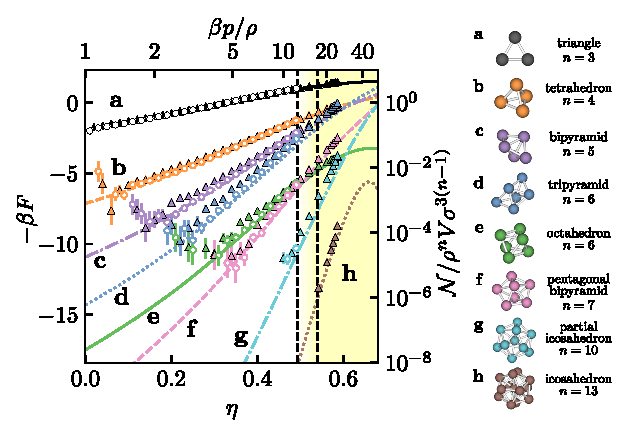
\includegraphics[width=\linewidth,center]{structure-populations}
  \caption[Concentration of local structures in the equilibrium liquid]{
    Static many-body structure in the hard sphere liquid: populations of small local structures in the hard sphere liquid determined from molecular dynamics simulations of 1372 monodisperse (open circles) and 8\% polydisperse (solid triangles) hard spheres against the theoretical prediction of this work (lines).
    Variations against volume fraction $\eta$ and compressibility $Z = \beta p/\rho$ shown.
    The hard sphere freezing and melting volume fractions are indicated by vertical dashed lines.
  }
  \label{fig:structure-populations}
\end{SCfigure}

To demonstrate the effectiveness of this approach we have taken structures for $3 \le n \le 13$ which are global minima of clusters in different simple liquids \cite{Wales2004}.
This set includes frustrated structures for $n \ge 7$ which do not correspond to rigid packings with unique energy minima; we will return to the rigid packings afterwards.
We selected these structures because we can identify them in molecular dynamics simulations using the algorithm of Ref.\ \cite{MalinsTCC2013}.
Using this algorithm we can compare the theoretical predictions against molecular dynamics simulations of both mono- and moderately polydisperse hard spheres at all volume fractions accessed by the simulations i.e.\ $\eta \lesssim 0.585$.
For the polydisperse simulations we used data from Ref.\ \cite{RoyallJSM2017} with a 5-component equimolar distribution with $\sim8\%$ polydispersity, to avoid freezing at high densities, and for the monodisperse simulations we used the DynamO software for event-driven molecular dynamics \cite{BannermanJCC2011}.
We determined their free energies using the thermodynamic integration steps outlined above.

In Fig.\ \ref{fig:structure-populations} we find excellent agreement between the theoretical prediction and the observed concentration of local structure seen in the simulations.
Our approach is able to predict populations of local structures well beyond the regime dynamically accessible to simulation, finding nontrivial structural change deep in the glassy regime highlighted by a rescaling with respect to the trivial $\rho^n$ density contribution.
The free energy of considered structures changes approximately linearly across the entire liquid regime, with deviations from linear becoming more apparent in the supercooled regime.

All structures apart from the fourfold symmetric octahedron in Fig.\ \ref{fig:structure-populations} are subunits of the icosahedron, and increase in concentration more rapidly than the octahedron until high density.
For $n=6$ we consider the free energies of two structures: the tripyramid and octahedron.
We find that the tripyramid occurs $\sim20$ times more often than the octahedron, their free energy difference being dominated by the different point group symmetries following \cite{MalinsJPCM2009,MengS2010}.
We can also estimate vibrational contributions, which allow us to match not only the relative but also the absolute values of free energies obtained from simulation.
In particular, we are able to capture the gradual reduction of the population of octahedral motifs in favour of the tripyramids at high volume fractions.
This is related to the previously observed emergence of fivefold symmetric motifs (such as the full and partial icosahedron) \cite{RoyallPR2015,TarjusJPCM2005,HallettNC2018,DunleavyNC2015}, which is here directly predicted from liquid state theory.

\begin{SCfigure}
  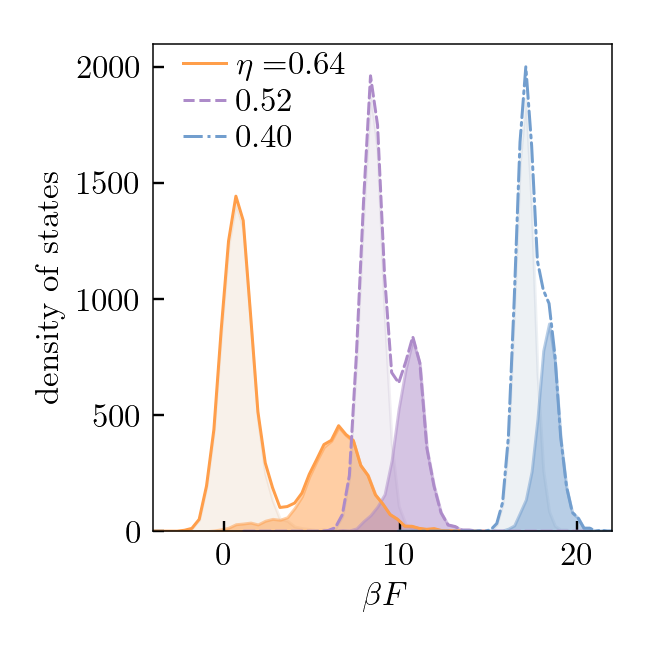
\includegraphics[width=0.9\linewidth,outer]{n12-dos}
  \caption[Free energy distribution of 12 particle structures]{
    Theoretical free energy distribution for the $n=12$ local library of states at several volume fractions.
    The distribution is shifted to lower energies at higher volume fractions, and develops an increasingly bimodal structure.
    Populations are decomposed into those structures containing pentagonal bipyramids without octahedra (light fill) and the remaining structures (dark fill).
  }
  \label{fig:n12-dos}
\end{SCfigure}

Having tested that the theory is accurate for selected geometries, we now take the exhaustive list of 11980 rigid structures for $n=12$ determined in Ref.\ \cite{Holmes-CerfonSR2016} to obtain a local density of states for a given sized inhomogeneity.
We calculated the free energy of all (first-order) rigid structures using \eqref{eq:local-structure-free-energy} (right panel of Fig.\ \ref{fig:structure-populations}), finding a bimodal distribution with two main peaks separated by a free energy difference that increases with increasing volume fraction.
We find the that lower energy distribution consists of structures rich in fivefold (icosahedral) symmetry in the absence of fourfold (octahedral) symmetry.
This shows that the hard sphere liquid is highly frustrated, and would be interpretted as the reason hard spheres make good glassformers in the geometric frustration picture \cite{KivelsonPA1995,TarjusJPCM2005}.
However, this result is potentially compatible with other thermodynamic scenarios like random first-order transition theory (RFOT) \cite{LubchenkoARPC2007}.

Each of the structures correspond to unique contact topologies, but in thermal systems (i.e. with finite gaps between particles) we expect many of them to be indistinguishable as found in Ref.\ \cite{TrombachPRE2018}.
As such, we have likely overestimated the height of the each peak, and especially the lower energy peak which contains more frustrated structures; we will find evidence of this in the next section.
Nevertheless, because this set of packings is exhaustive they represent a complete local density of states in the liquid, which is of fundamental interest to RFOT \cite{LubchenkoARPC2007}.
The distribution of energy levels is a key quantity, but to really examine the connection with dynamics we also need to know the \emph{connectivity} of the different energy states.
For this we need their reaction paths.

We used thermodynamic integration with Monte-Carlo methods to evaluate the free energies in this section, which cannot be straightforwardly applied along reaction paths.
Along reaction paths the geometries are saddles of the potential $\phi^{(n)}$, so the unstable direction must be excluded from integration.
In the next section we introduce analytical methods for evaluating the free energy to address this problem.

%As a Monte-Carlo method it would be very difficult to extend this method to saddles which is of great interest.
%Before moving on to our approximate analytical integration schemes we describe a method which is essentially exact to within numerical precision, at the cost of greater computational expense.

\section{Free energies along reaction paths}
\label{sec:reaction-paths}

While the thermodynamic integration techniques of the previous section are exact in principle, it is desirable to develop analytic approaches for evaluating the free energy.
Analytic approaches are typically faster which is desirable for dealing with larger $n$, as the number of possible packings appears to grow super-exponentially with particle number \cite{Holmes-CerfonSR2016}.
Moreover, analytic approaches are more readily able to calculate free energies along saddles, which are needed to obtain dynamical information in the vein of energy landscape approaches \cite{Wales2004}.

Two methods: assume no hard sphere interactions outside of the bonded particles, or Bayesian inference
\marginfootnote{In the current zeitgeist this could be construed as a form of machine learning; techniques for Bayesian inference are often thrown in with machine learning in e.g.\ topical reviews like Ref.\ \cite{MehtaPR2019}.
  Personally, I am hesitant to call this machine learning as the techniques more closely resemble the approximation schemes of traditional statistical mechanics (to me at least) than neural networks which have been driving the recent machine learning revolution.}

\begin{SCfigure}
  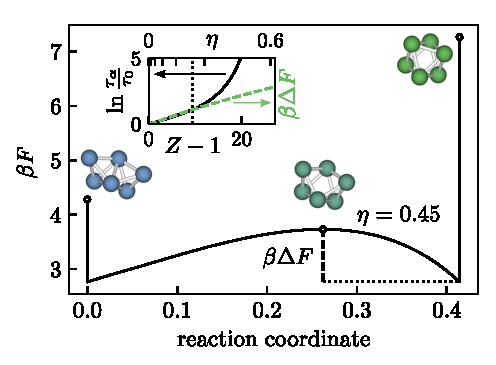
\includegraphics[width=0.9\linewidth,outer]{n6-reaction-path}
  \caption[The simplest nontrivial reaction path in hard spheres: octahedron to tripyramid]{
    Reaction for transition between tripyramid and octahedron $n = 6$ structures.
    Stationary points are indicated by markers: there is a discontinuity in free energy at the end points due to the additional integration over the reaction coordinate, and symmetry in the case of the octahedron.
    Inset: variation of activation barrier with volume fraction $\eta$ and compressibility $Z = \beta p/\rho$ from this theoretical reaction path (dashed line) and measured $\alpha$-relaxation times in bulk molecular dynamics simulations (solid line), where $\eta = 0.45$ is indicated with a vertical dotted line.
  }
  \label{fig:reaction-path-6}
\end{SCfigure}

We have thus far focused on static thermodynamic properties: yet a connection with dynamics can be made by calculating the free energy along reaction paths between (geometrically similar) structures.
This calculation along unstable directions in the free energy landscape requires an analytic approach (described in the SM), and generates paths such as the one in Fig.\ \ref{fig:reaction-path-6}.
Here we consider transitions between the tripyramid and the octahedron with $n=6$ because this is the simplest nontrivial transition between distinct hard sphere packings (SM).
Comparing this dynamical barrier to the structural relaxation for ($\alpha$-) relaxation timescale $\tau_\alpha$ extracted from simulations relative to a microscopic time $\tau_0$ (inset of Fig.\ \ref{fig:reaction-path-6}), we find this single reaction path barrier agrees with the low density scaling of $\tau_\alpha$ (linear in the compressibility factor $\beta p / \rho$ \cite{BerthierPRE2009}).
However, activated dynamics are not expected in this regime so this agreement may be coincidental.
%Moving to high densities, hard spheres exhibit two-step relaxation when vibrational ($\beta$--) and full ($\alpha$--) relaxations decouple as the system approaches its glass transition \cite{Berthier2011}.
%However, dynamics along the tripyramid--octahedron path continues to increase in an ``Arrhenius'' fashion quite unlike the super-Arrhenius increase exhibited by the $\alpha$--relaxation in the computer simulations (inset of Fig.\ \ref{fig:reaction}).
%It has been shown in molecular systems that $\beta$--relaxation can be Arrhenius in the deeply supercooled regime where $\alpha$-- relaxation is super-Arrhenius \cite{Yu2015}.
%Given that typical particle displacements in the tripyramid--octahedron path are around 0.15$\sigma$ per particle, we observe that this relaxation mechanism may be more characteristic of ($\beta$--) relaxation than full ($\alpha$--) relaxation.

\begin{SCfigure}
  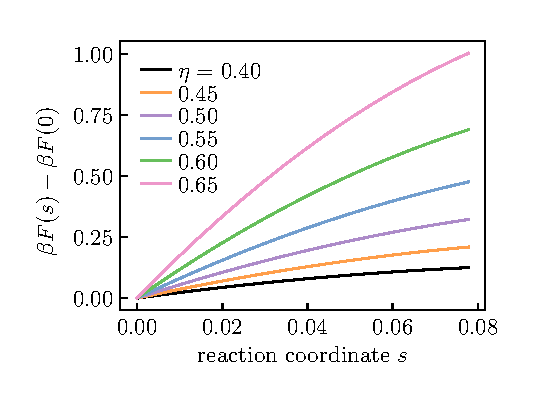
\includegraphics[width=0.9\linewidth,outer]{n7-reaction-path}
  \caption[Reaction path for the two variants of the frustrated pentagonal bipyramid]{
    Reaction for transition between the two $n = 7$ pentagonal bipyramids variant structures, from the variant with a broken spindle (bottom Fig.\ \ref{fig:packings}) to the variant with broken five-fold symmetry (top).
    The free energy increases monotonically along this reaction path, so there is no barrier separating these two structures.
  }
  \label{fig:reaction-path-7}
\end{SCfigure}

It is possible to extend our methodology for larger rearrangements, which may be sufficient to access ($\alpha$-) relaxation \emph{at very deep supercooling} for equilibrium systems.
\todo{Update this with the new Bayesian stuff.}
However, the rapid growth in the number of possible states presents a considerable numerical challenge requiring new methods and approximations, so we leave this exciting avenue for future study.

\section{Conclusions}

We have presented a formalism for describing many-body correlations in liquids and developed it into an accurate and computationally efficient parameter-free theory for hard spheres using integral geometry relying solely on the choice of the equation of state.
The key approximations involved treating the grand potential as continuous and additive (related to extensivity), and imposing the correct contact value of $g^{(2)}(r)$.
\todo{Change this to local structure.}

We applied the framework to a selection of local structural correlations, therefore predicting nontrivial changes in the energy landscape with supercooling putting previous empirical observations on more solid ground.
In particular, our analysis provides evidence for the existence of two populations of structures with distinct symmetries and free energies which causes the local density of states to become increasingly bimodal at high densities.
We note that we have treated densities corresponding to a degree of supercooling only accessible using novel swap Monte Carlo techniques \cite{BerthierPRL2016}; however, these simulations introduce large polydispersity, changing the local structure \cite{CoslovichJPCM2018} and thus limiting direct comparison with our calculations for the monodisperse liquid.

Our framework can be easily adapted to more complex liquids such as systems with soft repulsive interactions and polydisperse mixtures \cite{KodamaJCP2011}.
Integral geometry underlies the core approximation, so this approach can extend to hard particles of more complex shapes where the interaction potential is still geometric in nature.
\todo{Give link to the next chapter!}
It is applicable to a more general class of liquids where the soft part of the potential may be treated as a perturbation around a hard core \cite{Hansen2013} such that a geometric decomposition still applies.
This suggests a new route for predicting static properties of equilibrium liquids, with direct applications to self-assembly, nucleation and protein structure.

%% \section{New notes.}

%% We wish to describe local structure.
%% Ultimately, we wish to learn about the structure of the energy landscape in hard spheres.
%% To do so we must characterise the main features of the landscape, namely the different geometric packings and assign weights (free energies) to them.
%% This is a worthy goal in its own right, perhaps not that interesting for hard spheres but useful for wider applications (e.g.\ predicting self assembly, guiding chemical synthesis, understanding protein folding kinetics and predicting the native state and design).

%% The path we take is as follows:
%% \begin{enumerate}
%% \item We need some means of weighting points in the energy landscape: we do this using the morphometric approach (cf previous chapter)
%% \item A means of characterising and approximating the entire phase space: energy landscape formalism (next). This has two subgoals:
%%   \begin{enumerate}
%%   \item Divide the landscape into stationary points: minima and saddles.
%%     These stationary points characterise submanifolds of the entire landscape, \emph{basins} in the case of minima and \emph{reaction paths} in the case of saddles.
%%   \item Integrate over connected manifolds with weight function (potential of mean force) to obtain their free energies.
%%   \end{enumerate}
%% \end{enumerate}

%% %Another way of saying this is we need an integrand and boundary conditions.

%% \subsection{Connection with energy landscape descriptions}

%% \begin{itemize}
%%   \item First describe the energy landscape description.
%%   \item Based on low-temperature expansion arguments.
%%   \item Mean-field: Laplace method/saddle-point.
%%   \item Gaussian expansion around this result (called Harmonic approximation in energy landscape/chemistry literature).
%% \end{itemize}

%% %% \begin{SCfigure}[H]
%% %%   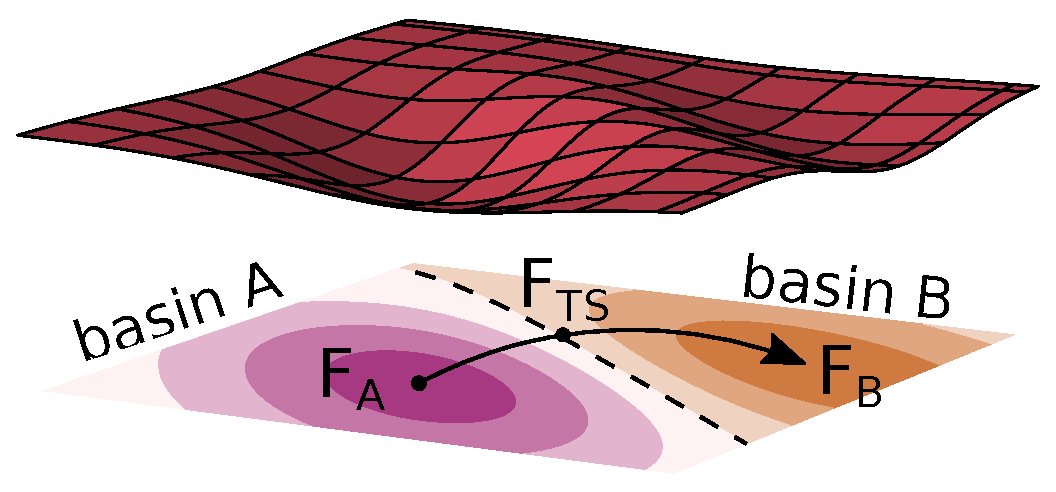
\includegraphics[width=\linewidth,outer]{toy-landscape}
%% %%   \caption[A cartoon energy landscape]{A cartoon energy landscape for a 2-dimensional phase space.
%% %%     The landscape features two local minima: $A$ and $B$.
%% %%     The area surrounding each minima defines its basin: any point from which the minima can be found by moving downhill belongs to the basin.
%% %%     Energy landscape approach: at low temperatures the system is expected to oscillate around potential energy minima, so the dynamics can be understood as rare events causing a change of basin.
%% %%     Thus a decomposition of the phase space in terms of basins should become exact for the dynamics at low temperatures in the supercooled regime of interest.}
%% %% \end{SCfigure}

%% In the case of local arrangements of hard spheres, rigid packings seem to correspond to minima of the potential of mean force.
%% I cannot prove this for the case of morphometric approach, but I cannot find a counter example.
%% Possibly can prove they are minimal volume.

%% \section{Locally favoured structures in hard spheres}

%% \section{Introduction}

%% This study builds on and contributes to work in nonequilibrium statistical physics, particularly relating to glasses and nucleation.
%% Although small-system studies have examined how dynamics are influenced by topographical properties of the energy landscape for simple systems, there has not been a systematic formalism for extending this to the bulk liquid.
%% As such, this study provides additional insight into dynamical arrest i.e.\ the supercooled liquid and glasses.

%% The analytic focus on many-body correlations provides another contribution to the fundamental understanding of simple liquids.
%% This study analyses depletion forces in order to predict the many-body correlation functions in the bulk liquid.
%% Although numerous studies have identified the role of local structure in dynamical arrest little analytical attention has been paid to how to properly formulate structure in a quantitative thermodynamic framework.
%% I address this issue by expressing the solvation free energies in terms of geometrical properties of a small solute, and develop techniques for making quantitative predictions of local structure in the hard sphere liquid.

%% Energy landscape can be divided into two strands: the topographic view of Stillinger which offers a powerful conceptual tool for understanding complex phenomena.
%% At low temperatures we can imagine the system oscillating around low energy minima (inherent states), with occasional large fluctuations driving it through `choke points' causing a change to a different energy minimum.
%% This formalism was turned into a properly quantitative framework by Wales \cite{Wales2004,?}, where stationary point databases are constructed: energy minima connected by saddles.
%% From the connectivity of the landscape one can understand dynamical arrest: if there are lots of competing low lying minima it can be hard for the system to find the global minimum and we expect it to fall out of equilibrium easily when temperature is lowered.
%% By contrast, if the minima steadily lower in energy then they act as a funnel to the global minimum so we expect rapid equilibration.

%% Quantitative predictions are typically only possible for small systems, so it is desirable to extend it to the bulk.
%% One can to do this focusing on a subset of the total degrees of freedom, integrating out the rest in an approximate fashion.
%% The selected degrees of freedom act as a small system with a many-body interaction potential, so can be treated with the aforementioned formalism in a quantitative manner.
%% This was attempted by Tarjus \cite{?} with mixed success.
%% The morphometric approach \cite{KonigPRL2004,RothPRL2006,RobinsonPRL2019} offers a generic framework to treat many-body correlations allowing a first-principles treatment of local structure in the bulk liquid.
%% This framework is accurate for hard spheres where it has been extensively tested \cite{Hansen-Goos?,Roth?,Bob?,RobinsonPRL2019}.

%% Hard particle systems are the fundamental system of interest for simple liquids.
%% The stationary point database approach, firmly rooted in \emph{potential energy}, fails for hard systems as the potential energy is trivial so the thermodynamics is athermal.
%% It has never been extended to hard systems until now.
%% This extension comes with the cost that some of the elegant techniques of soft systems will fail due to the singular nature of hard sphere interactions, so we require new methods to handle the idiosyncrasies of hard systems.
%% Here we propose a practical definition for basins when working with hard systems, and develop techniques for evaluating thermodynamic quantities with this definition.
%% We then retroactively justify the meaningfulness of this basins by comparing with simulation/literature data.

%% \todo{Talk about the past work on hard spheres: penny packing, and sticky spheres.}
%% A number of unique technical challenges brought about by the hard sphere potential, that we will solve.
%% The groundwork for this was laid down by Holmes-Cerfon and coworkers.
%% Note: attempts have been successful at modelling effective interactions close to isostaticity where $z \to 2d$.
%% This is empirically found to be the case asymptotically as one approaches jamming, however it is worth noting that there is no general requirement that $z = 2d$ for rigid packings, and counter examples where $z < 2d$ are known.

%% In section \ref{sec:energy-landscapes} we review the energy landscape formalism for soft potentials, with a view to highlighting where it might fail for hard interactions.
%% We review the liquid state theory/morphological approach used for treating the depletion interactions between hard particles in the bulk liquid in section \ref{?},
%% followed by the equivalent of the partition function for local structure.
%% Our core theoertical results are then presented in section \ref{?}, where we propose a definition of local structure and show techniques for evaluating the partition function nonperturbatively.
%% We then present the results of the topography of the local structural energy landscape in hard spheres in section \ref{?}, our main numerical results.

%% \section{Energy landscape approaches}
%% \label{sec:energy-landscapes}

%% Points to cover:
%% \begin{itemize}
%% \item Give a technical definition of local structure with a goal to showing the problems with hard systems.
%% \item Define structures as manifold: $\mathbb{R}^{dn}$ for $n \ll N$, embedded in $\mathbb{R}^{dN}$
%% \item Failure of perturbation theory due to singularity of
%% \end{itemize}

%% The energy landscape/inherent structure approach is a powerful theoretical framework for understanding complex phenomena.
%% At its core, it is a means of coarse-graining the high dimensional phase space into a more manageable mesostates.
%% Its power comes from the fact that it is essentially exact, though calculations are typically intractable unless the degrees of freedom can be significantly reduced; in practice this is generally only possible in mean field (high spatial dimensions) or for small systems $N = \mathcal{O}(10)$ in physical settings.
%% The approach is however useful conceptually for developing theories based around the topography of the energy landscape \cite{Stillinger}, and makes detailed calculations tractable typically for small systems \cite{Wales2004}.

%% In this section we will review the energy landscape approach, how it applies to soft potentials and the complications that arise for our system of interest: hard spheres.
%% First we talk about coarse-graining into mesostates mentioned above, whether into inherent structures or otherwise.
%% A mesostate is a collection of microstates which are grouped together, typically these are selected for sharing some desirable property to simplify description.
%% For practical reasons this means that microstates should be connected in phase space so they are compact manifolds.
%% In connection with the topographic view we will call these manifolds \emph{basins}.
%% The total partition function is then decomposed as
%% \begin{equation}
%%   Z \equiv \int_{\mathbb{R}^{dN}} e^{-\beta (U_N(\vec{r}^n) + \phi(\vec{r}^n))} \, d\vec{r}^N = \sum_i Z_i
%% \end{equation}
%% where $\phi$ is the external potential of the container in order to keep the particles localised in a region where they interact.
%% Alternatively they could be embedded in a toroidal topology to prevent particle dissociation (as in e.g.\ simulations with periodic boundary conditions).
%% The basin partition function is
%% \begin{equation}
%%   Z_i = \int_{\mathbb{V}_i^{dN}} e^{-\beta U_N(\vec{r}^N)} \, d\vec{r}^N
%% \end{equation}
%% if $\mathbb{V}_i^{dN} \subset \mathbb{R}^{dN}$ is the manifold corresponding to basin $i$.
%% One can define (e.g.\ Wales).
%% Despite a definition which unambiguously demarcates the basins, the high dimensionality of the phase space renders the integrals in \eqref{eq:basin-partition-function} completely intractable without approximation.

%% The equilbrium probability of the system being in basin $i$ at any one time is thus
%% \begin{equation}
%%   p_i = \frac{Z_i}{Z}
%% \end{equation}
%% From the Gibbs-Shannon entropy we find the coarse-graining entropy
%% \begin{equation}
%%   \begin{split}
%%     S_{\textrm{conf}}
%%     &= -\sum_i p_i \ln{p_i} \\
%%     &= -\sum_i \left( \frac{Z_i}{Z} \ln{Z_i} - \frac{Z_i}{Z} \ln{Z} \right) \\
%%     &= \ln{Z} - \sum_i \frac{Z_i}{Z} \ln{Z_i}
%%   \end{split}
%% \end{equation}
%% Noting that the total free energy is $F = -k_B T \ln{Z}$ we thus have
%% \begin{equation}
%%   \beta F = \langle \beta F_i \rangle - S_{\textrm{conf}}
%% \end{equation}
%% where the average basin free energy $F_i = -k_B T \ln{Z_i}$ is
%% \begin{equation}
%%   \langle \beta F_i \rangle = - \frac{1}{Z} \sum_i Z_i \ln{Z_i}
%% \end{equation}

%% Finally, we have to choose how to define the basins.
%% In the energy landscape approach the coarse-graining occurs around local minima of energy where $\vec{\nabla}U_N = 0$ and Hessian $\frac{1}{2}\vec{\nabla}\vec{\nabla}U_N$ is positive definite.
%% Each basin consists of all the points connected by a steepest descent path to a unique energy minimum.
%% This description reduces the high dimensional continuous description down to discrete number of zero-dimensional manifolds.
%% In practice the number of minima scales exponentially in $N$, so this is still an intractably large number of points.
%% One can even obtain dynamical information by considering the saddles, i.e.\ the unstable stationary points.
%% The saddles act as the lowest (in energy) lying points that must be crossed to jump from one basin to another, giving the energy barriers to dynamics.

%% How do we justify this approach?
%% Energy is smooth so asymptotics around stationary points is valid: inherent state (stable stationary points) description
%% For infinite systems we could use Laplace method
%% \begin{equation}
%%   \int_{\mathbb{V}^{dN}_i} e^{-\beta N u_N(\vec{r}^N)} \, d\vec{r}^N
%%   \sim
%%   e^{-\beta \min{U_N(\vec{r}^N)}} \qquad \forall \; N \gg 1
%% \end{equation}
%% where $u_N = U_N / N$.
%% For finite systems we could go beyond this pertubatively by employing a harmonic approximation from the energy-landscape literature
%% \begin{equation}
%%   U_N = U_N(\vec{p}_i) +
%%   \frac{1}{2} \Delta \vec{r} \cdot \left. \nabla \nabla U_N\right|_{\vec{p}_i} \cdot \Delta \vec{r}
%%   + \mathcal{O}(\Delta \vec{r}^3)
%% \end{equation}
%% where \[\vec{p}_i = \argmin_{\vec{r}^n \in \mathbb{V}_i^{dN}}{\left(U_N(\vec{r}^n)\right)}\] is the location of the energy minimum.
%% \begin{equation}
%%   Z_i \sim \exp{-\beta U_N(\vec{p}_i)}
%% \end{equation}
%% There are two layers of approximation: first we model the pdf as a Gaussian, second we approximate the boundary conditions as being infinite.
%% The inclusion of the Hessian term in the expansion around the minimum shows that for soft potentials one can perturbatively build a description around the inherent states.
%% At low temperatures this approach is expected to become exact (for the first layer not the second one).
%% So for athermal systems perturbation theory should break down.

%% \begin{SCfigure}
%%   \missingfigure[figwidth=\linewidth]{}
%%   \caption{Failure of Laplace method for hard interactions.}
%% \end{SCfigure}

%% To make the above discussion concrete we will consider two examples.
%% First, we examine a symmetric quartic potential
%% \begin{equation}
%%   \phi = \epsilon (x^4 - x^2)
%% \end{equation}
%% where $x$ is some state variable and $\epsilon$ is an energy scale.
%% This could represent e.g.\ a ferromagnet below the critical temperature with $x$ representing the spontaneous magnetisation.
%% The free energy in units of $\epsilon$ is then
%% \begin{equation}
%%   F = - T \ln{\left( \int \exp{\left(-\frac{\phi}{T}\right)} \, dx \right)}
%% \end{equation}
%% This potential naturally contains two basins for the two half space $x \in [-\infty, 0]$ and $x \in [0, \infty]$, and because of the symmetry of the potential around $x=0$ the contribution of each of these basins is identical, i.e.\
%% \begin{equation}
%%   Z = 2 \int_0^\infty \exp{\left(-\frac{\phi}{T}\right)} \, dx.
%% \end{equation}
%% Applying the harmonic approximation
%% \begin{equation}
%%   \begin{split}
%%   Z &\simeq
%%   2 \exp{\left( -\frac{\phi(x_0)}{T} \right)}
%%   \int_{-\infty}^\infty \exp{\left(-\frac{\phi''(x_0)}{2T}\right)} \, dx \\
%%   &=
%%   2 \exp{\left( -\frac{\phi(x_0)}{T} \right)}
%%   \sqrt{\frac{2 \pi T}{\phi''(x_0)}}
%%   %+ \mathcal{O}(\phi'''(x_0))
%%   \end{split}
%% \end{equation}
%% where $x_0 = \dfrac{1}{\sqrt{2}}$ is the position of the minimum in the $x > 0$ basin.

%% To summarise this section, we note that the basin definition of structures for soft potentials has the properties that: \cite{Wales?}
%% \begin{itemize}
%% \item Each basin $B_i$ connects to a unique minimal energy state with a unique geometry.
%% \item Divide the phase space into basins which do not overlap $B_i \cap B_j = \emptyset$ for $i \ne j$ and tile the whole of phase space $\cup_i B_i = \mathbb{R}^q$.
%% \item Its free energy is well-defined (at least in some asymptotic limit) so it can be approximated with simple methods.
%%   For soft potentials this is a consequence of the first criterion.
%%   This makes the choice of coarse-graining (thermo)dynamically meaningful: it is long-lived enough that the microstates making up a basin can be not distinguished, and the dynamics reduces to basin crossing events.
%% \end{itemize}
%% A definition satisfying the first two criteria is possible, however due to the singularity in the hard particle interaction potential the region surrounding the (depletion) energy minimum is thermodynamically irrelevant.
%% This can be interpretted:
%% \begin{itemize}
%% \item \emph{Thermodynamically}: the region near contact is entropically suppressed, regions away from contact have many more microstates so are entropically enhanced
%% \item \emph{Dynamically}: as hard spheres approach one another they collide and bounce away so spend infinitesimally small timescales at contact.
%%   Collisions almost universally involve only two particles, collisions of more than two particles occur with zero measure.
%% \end{itemize}
%% Because of this we cannot obtain the free energy by a small parameter expansion around the contact point.
%% We must evaluate the full integral over a finite volume.
%% To make this tractable we will abandon the rigorous definition of structures in terms of basins employed for soft potentials, in favour of a simple one based on intuitive geometrical ideas.
%% We will later explore the limitations/successes of this definition in order to retroactively justify this approach.

%% Due to the analogies between the population/concentration integral and the usual partition function, we will refer to this integral simply as a partition function.

%% \subsection{Molecular partition function}

%% From the definition of the probability density function in Eq.\ \eqref{eq:n-density-pdf}, the total number of local structures of a particular type in a volume $V$ is
%% \begin{equation}\label{eq:structure-population}
%%   \mathcal{N} =
%%   \int_{\mathcal{Q}} \rho^n g^{(n)}(\vec{r}^n) \, d\vec{r}^n,
%% \end{equation}
%% where $\mathcal{Q}$ is the domain \emph{defining} the local structure.
%% To get the free energy expression used in the main text we consider the manifold diffeomorphic to translations, defining $\mathcal{Q} = \mathcal{D} \rtimes \mathbb{V}$ where $\mathbb{V}\subset \mathbb{R}^3$ is the system volume.
%% Exploiting translational invariance of the potential of mean force, we fix one particle at the origin and integrate the center of mass over the system volume giving
%% \begin{equation}
%%   \mathcal{N} =
%%   \rho^n V \int_{\mathcal{D}} g^{(n)}(\vec{r}^n) \, d\vec{r}^{n-1}.
%% \end{equation}
%% We defined a free energy by taking $\mathcal{N} = \sigma^{3(n-1)} \rho^n V e^{-\beta F}$, which together with the above expression gives Eq.\ \eqref{eq:local-structure-free-energy} in the main text.

%% There will be $d$ translation modes and $\frac{d(d-1)}{2}$ rotational modes for each plane formed by pairs of coordinate axes (e.g.\ $x^1 \wedge x^2$ for rotations in the $x^1x^2$-plane).
%% Subtracting the number of rigid body modes from the total degrees of freedom gives \[ q = dn - \frac{d(d+1)}{2} \] internal degrees of freedom.
%% Exception when rotations are degenerate: $n < d$ (e.g.\ $n=2$ in $d=3$) or pathological cases of unusually high symmetry (e.g.\ when all particles fall on a line) which can in general be excluded.

%% More generally, we consider the manifold diffeomorphic to translations \emph{and} rotations.
%% We define $\mathcal{Q} = \mathcal{D}' \rtimes SE(3)$ where $\textrm{SE}(d)$ is the $d$-dimensional special Euclidean group, leaving the $\mathcal{D}'$ as the space of the structure's internal motion.
%% We separate rigid body from internal motion by applying the following transformation to each particle coordinate
%% \begin{equation}
%%   \vec{r}(\{\vec{t}, \vec{\theta}, \vec{x}\}) =
%%   \vec{t} + \vec{R}(\vec{\theta}) \cdot \vec{q}(\vec{x}),
%% \end{equation}
%% where $\vec{t}$ is the translation vector, $\vec{\theta}$ the Euler angles, $\vec{R}$ the rotation matrix, and $\vec{x} \in \mathbb{R}^{3n-6}$ represents the internal coordinates.
%% We need to compute the metric of this transformation $G_{ij} = \vec{G}_i \vec{G}_i^T$ where the (generally curvilinear) basis vectors are $\vec{G}_i = \partial_i \vec{r}$.
%% To simplify calculation we choose $\vec{q}(\vec{x})$ to always be in the center-of-mass frame and orthogonal to rotations such that $G_{ij}$ reduces to block-diagonal form.
%% If the rotation matrix is expressed in Euler-angle representation as $\vec{R}(\vec{\theta}) = \vec{R}_3(\theta_3) \vec{R}_2(\theta_2) \vec{R}_1(\theta_1)$ then we have%
%% \footnote{While the final form of $\vec{G}$ is elegant, I do not have a straightforward way of getting it; it involved a lot of guesswork and within Mathematica to find a form of $\vec{U}$ which gives the middle block.
%%   There is probably a more direct route.}
%% \begin{equation}
%%   G_{ij}(\{\theta_i\}, \vec{x}) =
%%   \begin{pmatrix}
%%     n \vec{E} & 0 & 0 \\
%%     0 & \vec{U}^T(\vec{\theta}) \vec{M}(\vec{x}) \vec{U}(\vec{\theta}) & 0 \\
%%     0 & 0 & \overline{G_{ij}}(\vec{x})
%%   \end{pmatrix},
%% \end{equation}
%% where $\vec{E}$ is the identity matrix, $\vec{M}$ is the moment of inertia tensor, $\overline{G_{ij}}$ is the metric for internal motion, and we have defined the matrix $\vec{U}$ as
%% \begin{equation}
%%   \vec{U}(\vec{\theta}) =
%%   \begin{pmatrix}
%%     1 &  0              & -\sin{\theta_2} \\
%%     0 &  \cos{\theta_1} &  \cos{\theta_2} \sin{\theta_1} \\
%%     0 & -\sin{\theta_1} &  \cos{\theta_2} \cos{\theta_1} \\
%%   \end{pmatrix}
%%   \qquad
%%   \begin{aligned}
%%     \theta_1 &\in [0,2\pi] \\
%%     \theta_2 &\in \left[-\frac{\pi}{2},\frac{\pi}{2}\right] \\
%%     \theta_3 &\in [0,2\pi].
%%   \end{aligned}
%% \end{equation}
%% Note $\det{\vec{U}} = \cos{\theta_2}$.
%% The volume element in the new coordinates is
%% \begin{equation}
%%   d\vec{r}^n = \frac{\sqrt{\det G_{ij}(\vec{x})}}{\nu}
%%   \, d^3 \vec{t} \, d^3 \vec{\theta} \, d^{3n-6} \vec{x},
%% \end{equation}
%% where $\nu$ is the symmetry number (discussed below) and
%% \begin{equation}
%%   \sqrt{\det G_{ij}(\vec{x})} =
%%   \cos{\theta_2} \sqrt{\det{\vec{M}(\vec{x})}}
%%   \sqrt{n^3 \det{\overline{G_{ij}}(\vec{x})}}.
%% \end{equation}
%% The symmetry number emerges as the choice of internal coordinates typically fixes the particle labels breaking permutation symmetry; we have to multiply by the $n!$ possible labellings, which introduces double counting if the structure possesses rotational symmetry so we have to divide by the correcting factor $\nu$.
%% This is explained in detail in Ref.\ \cite{CatesSM2015}.
%% Thus \eqref{eq:structure-population} reduces to
%% \begin{equation}\label{eq:structural-partition-function-detailed}
%%   \frac{\mathcal{N}}{\rho^n V}
%%   =
%%   \frac{8\pi^2 \sqrt{n^3}}{\nu} \int_{D'}
%%   g^{(n)}(\vec{x}) \,
%%   \sqrt{\det{\overline{G_{ij}}(\vec{x})} \det{\vec{M}(\vec{x})}}
%%   \, d^{3n-6} \vec{x}.
%% \end{equation}
%% Note that in the limit of linear molecules, i.e.\ where all particles fall on a line, the above approach fails as there is one less rotation mode requiring a modified description.

%% Note that for all of the geometries we have tested this metric seems to be 2, although we could not prove this is in the general case.
%% We have to actually evaluate the integral.
%% We will explore thermodynamic integration using Monte Carlo, which is essentially exact to numerical precision but slow, and some analytical approximations.

%% \subsection{Worked examples}

%% %% \begin{SCfigure}
%% %%   \missingfigure[figwidth=\linewidth]{}
%% %%   \caption{Number of first shell neighbours in the hard sphere liquid.}
%% %% \end{SCfigure}

%% %% \begin{SCfigure}
%% %%   \missingfigure[figwidth=\linewidth]{}
%% %%   \caption{Number of equilateral triangles in the hard sphere liquid.}
%% %% \end{SCfigure}

%% We will consider two worked examples for simple geometries which are readily visualised and for which the metric $G(\vec{x})$ is known exactly and the partition function integral reduces to a simple form.

%% Our first worked example is at the two-body level: the typical number of neighbours in the first shell.
%% For a dimer the metric term evaluates to $G(\vec{x}) = r^2$, i.e.\ the usual spherical coordinate Jacobian as expected.
%% The average number neighbours less than some distance $r$ is then
%% \begin{equation}
%%   z(r)
%%   = 4\pi \int_0^r g^{(2)}(r) r^2 \, dr
%%   = 4\pi \int_\sigma^r e^{-\beta \phi^{(2)}(r)} r^2 \, dr
%% \end{equation}
%% This is a common measurement where $r$ is taken up to the first minimum of the $g(r)$ then $z$ corresponds to the number in the ``first-shell'' (i.e. the coordination number).

%% Our second worked example considers the average concentration of triangles in the liquid.
%% Here the relevant coordinates are the tuple $\vec{x} = (r,s,t)$ where the three distances are the lengths of the triangle.
%% The metric has previously been determined exactly as $G(\vec{x}) = rst$ in \cite{?}.
%% The number of equilateral triangles with maximum side length $\delta$ is then
%% \begin{equation}
%%   N_\Delta(\delta)
%%   =
%%   8\pi^2 \int_\sigma^\delta\int_\sigma^\delta\int_\sigma^\delta
%%   e^{-\beta\phi^{(3)}(r,s,t)} rst \, dr ds dt.
%% \end{equation}
%% The results show excellent agreement with molecular dynamics simulations across the entire liquid regime, and even into the supercooled regime where simulations are available for a polydisperse system.

%% \section{Results}

%% We take the minimal energy structures as the stable packings determined in Refs.\ \cite{ArkusPRL2009,Holmes-CerfonSR2016}.
%% For each landscape with $n \le 5$ there is only a single stable packing, i.e.\
%% \begin{itemize}
%% \item Dimer $n=2$
%% \item Equilateral triangle $n=3$
%% \item Tetrahedron $n=4$
%% \item (Triangular) bipyramid $n=5$
%% \end{itemize}
%% However for $n = 6$ we first see two competing packings: the tritetrahedron and the octahedron.

%% At $n = 7$ there are 5 stable packings, including two subgraphs of the pentagonal bipyramid each with a broken bond: one has a broken spindle, the other a broken ring.
%% This is a well known property of hard sphere packings, and the cause of geometric frustration: it is generally well-established \cite{?,?,?,Robinson?} that 5-fold symmetric structures are lower in (free) energy for simple systems, however they do not tile space perfectly leading to the suppresion of long-range ordering.
%% For soft systems this frustration can be overcome and all of these `contraints' can be satisfied \cite{Frank,Wales}.
%% However, if we look at the one-dimensioinal reaction paths for n=7 we see that there is not thermal barrier separating these two structures.
%% This shows that they should not be distinguished in the liquid regime, showing the limitation of our definition of structure: they are simply thermal fluctuations of one another.
%% We have overcounted the number of stable structures for $n=7$ by one.
%% For similar reasons we have likely overestimated number of structures in n = 12 landscape, but does not change the fact that they are lower in energy

%% Comparing accuracy of analytical integration methods, we find a systematic error increasing with volume fraction likely due to the perturbation in the potential of mean force.
%% For most of the structures the error scales with a similar magnitude and the same sign (see Fig.\ \ref{?}), suggesting a systematic error.
%% Numerical experiments for $g^{(3)}$ show that the main source of error is the order of the expansion, with second-order significantly improving it and third-order being essentially exact.
%% We cannot distinguish the result with the true metric from the that with the approximate metric: this is not a big source of error, at least not for $n=3$ where we can test it.

%% However for a subset of the structures we find that the error has the opposite sign, due to a different source of error: the neglect of additional hard sphere interactions.
%% \todo{Collapse all the data onto a single figure.
%%   Can we rescale the error by the free energy?
%%   What can we correlate?}
%% Using expectation propagation the sign of the error is restored showing that we are treating these interactions, though the error is generally larger than for the other structures as it is not an exact method.
%% \todo{Can we include the potential expansion to second order?}

%% \begin{SCtable}
%%   \begin{minipage}[b]{\linewidth}
%%     \centering
%%     \begin{tabular}{cccc}
%%       Structure & $\beta F(\eta=0.45)$ & $\beta F(\eta=0.56)$ & $\beta F(\eta=0.64)$ \\
%%       \hline
%%       1 & 0.5 & 0.7 & 0.9 \\
%%       2 & 0.5 & 0.7 & 0.9 \\
%%       3 & 0.5 & 0.7 & 0.9 \\
%%       4 & 0.5 & 0.7 & 0.9 \\
%%       5 & 0.5 & 0.7 & 0.9 \\
%%     \end{tabular}
%%   \end{minipage}
%%   \caption{Free energies of structures for $n=7$ landscape at varying volume fractions.}
%% \end{SCtable}

%% \begin{SCfigure}
%%   \missingfigure[figwidth=\linewidth]{}
%%   \caption{Distribution of energy levels for $n \le 9$.
%%   Include saddles.}
%% \end{SCfigure}

%% \begin{SCfigure}
%%   \missingfigure[figwidth=\linewidth]{}
%%   \caption{Distribution of energy levels for $10 \le n \le 12$.}
%% \end{SCfigure}

%% Next we give the minimal energy structures for $8 \le n \le 12$.

%% \section{Discussion}

%% Here we summarise our many layers of approximations.
%% First, we have to make a \emph{choice} over how to coarse-grain the phase space.
%% This is not strictly an approximation, but it defines what we mean by a `structure' and informs the approximations used to compute the free energies.
%% Then, we make the following approximations:
%% \begin{enumerate}
%% \item Morphological approach for correlations:
%%   \begin{enumerate}
%%   \item Morphometric \emph{ansatz}
%%   \item Virial choice of closure with Carnahan-Starling equation of state
%%   \end{enumerate}
%% \item Expansions of geometrical measures:
%%   \begin{enumerate}
%%   \item Second-order expansion of geometric measure (i.e.\ moment of inertia)
%%   \item Contact measure for bond-distance space (i.e.\ zeroth-order term): this seems to be more or less exact for $n=3$
%%   \end{enumerate}
%% \item First-order expansion of potential around contact (can we get second?)
%% \item Polyhedral approximation of boundary conditions (additional hard sphere bonds).
%% \item Bayesian inference to perform integral
%% \end{enumerate}
%% \todo{Mention how we nudge the coordinates with a small perturbation from the contact point to prevent problems with e.g.\ four-particle intersections (and higher)}

%% We found that two 5-fold symmetric structures at $n=7$, both pentagonal bipyramids with broken symmetries, are not separated by a thermodynamic barrier.
%% This means they should be considered as thermal fluctuations of one another, and not be distinguished.
%% This explains why 5-fold symmetric structures like the icosahedron are thermally stable in the hard sphere liquid.
%% Note that at jamming the symmetry of these structures must be broken.

\ifdefined\includebibliography
  \newgeometry{margin=1in}
  \printbibliography
\fi

\end{document}

%TC: macro \marginfootnote [other]
%TC: envir SCfigure [] other
%TC: macrocount beginSCfigure [figure]
\documentclass[11pt,twoside]{report}
\usepackage{preamble}
\setcounter{chapter}{4}
\graphicspath{{../img/}}
\def\includebibliography{}

\externaldocument{background}

\begin{document}
\chapter{Morphological thermodynamics for hard bodies from a controlled expansion}
\epigraph{He said that the geometry of the dream-place he saw was abnormal, non-Euclidean, and loathsomely redolent of spheres and dimensions apart from ours.}{H.\ P.\ Lovecraft, \emph{The Call of Cthulhu} (1926).}
\label{chapter:resummation}

\section{Introduction}

The standard theoretical framework for treating inhomogeneous liquids is classical density functional theory (DFT).
Central to this theory is the result that the free energy can be \emph{exactly} expressed as a functional of the density $\Omega = \Omega[\rho(\vec{r})]$ \cite{EvansAP1979}, though approximate functionals must be used in general.
For example, the fundamental measure theory (FMT) \cite{RosenfeldPRL1989} provides a class of highly accurate functionals for the hard sphere liquid.
% relying on physical ingenuity.
A common practical application of DFT is to its \emph{dual} problem: determining the free energy $\Omega = \Omega[\phi_\mathrm{ext}(\vec{r})]$ for a fixed external potential $\phi_\mathrm{ext}(\vec{r})$.
Approaching this through DFT requires minimisation of $\Omega$ to obtain the equilibrium density profile, a tractable but expensive procedure.
In situations where many function evaluations are required, e.g.\ when integrating over many different realisations of $\phi_\mathrm{ext}$, this minimisation operation can become prohibitively expensive.
It is worthwhile to investigate more direct routes to approximating $\Omega[\phi_\mathrm{ext}(\vec{r})]$, especially where accuracy may be less important than fast calculation.

A promising approach to the dual problem is through morphological thermodynamics \cite{KonigPRL2004} with the potential to enable fast and accurate calculations in hard spheres \cite{RothPRL2006,Hansen-GoosPRL2007,RobinsonPRL2019}.
The morphometric approach concerns sharply repulsive external potentials where $\phi_\mathrm{ext}$ acts as a container for the fluid or as an exclusion volume for e.g.\ a solute.
In this limit the density profile is negligible over a volume $V$, and the free energy is expanded in terms involving $V$ and its boundary $\partial V$.
In this approximation the free energy change from its homogeneous value $\Delta \Omega := \Omega[\phi_\mathrm{ext}] - \Omega_\mathrm{hom}$ is expanded as
\begin{equation}\label{eq:morphometric-approach}
  %\Omega[\phi_\mathrm{ext}] - \Omega_\mathrm{hom}
  \Delta \Omega
  =
  p V + a_2 A + a_1 C + a_0 X,
\end{equation}
where $p$ is the pressure and $\{a_2,a_1,a_0\}$ are coefficients for the surface terms $A$, the area; $C$, the integrated mean curvature; and $X$, the integrated Gaussian curvature.
The surface terms are normally determined from the integrals
\begin{subequations}
  \begin{align}
    A &= \int_{\partial V} \, dA \\
    C &= \frac{1}{2} \int \Tr{\kappa} \, dA \\
    X &= \int_{\partial K} \det{\kappa} \, dA
  \end{align}
\end{subequations}
where $\kappa$ is the curvature tensor on the surface.

Despite its accuracy in hard spheres the morphometric expansion \eqref{eq:morphometric-approach} is still an approximation, as numerous detailed investigations have shown \cite{OettelEL2009,AshtonPRE2011,LairdPRE2012,BlokhuisPRE2013,UrrutiaPRE2014,Hansen-GoosJCP2014}.
Fundamental questions remain over \emph{why} it is accurate and how one might improve the approximation.
Inaccuracies become significant in hard spheres at very high densities approaching the glass transition \cite{RobinsonPRL2019,RobinsonPRE2019}, so an approximation scheme including additional terms could be desirable for approaches to dynamical arrest.
An important feature of the geometric terms in the morphometric approach is that they remain well defined even where a curvature tensor is not locally definable, at e.g.\ a cusp; this property is central to the success of the expansion \eqref{eq:morphometric-approach} so that the coefficients can be independent of the geometry.
Correspondingly, proposed approximations of $\Omega[\phi_\mathrm{ext}(\vec{r})]$ which do not share this feature can be ruled out as general expansions.

To illustrate this we consider what happens if one attempts to extend \eqref{eq:morphometric-approach} by including higher moments of curvature.
A prototypical example of this is the \emph{Helfrich expansion} for elastic membranes \cite{HelfrichZFNC1973}, which is often argued to be the most general expansion for the surface tension.
The next highest order term to augment \eqref{eq:morphometric-approach} would be
\begin{equation*}
  \int_{\partial V} \left(\Tr{\kappa}\right)^2 dA,
\end{equation*}
which is not well-defined for general surfaces, in particular for surfaces containing vertices and/or arcs as occurs in e.g.\ polyhedra.
To demonstrate this we consider the line where two planes intersect with dihedral angle $\Delta \theta$.
This can be considered as a cylindrical sector in the limit of vanishing radius $r$, giving the contribution per unit length
\begin{equation*}
  \int \left(\Tr{\kappa}\right)^2 r d\theta
  = \frac{\Delta \theta}{r}
\end{equation*}
diverging as $1 / r$ in the limit where the sector becomes an arc $r \to 0$.
We find that only the curvature terms already present in the morphometric approach are well-defined in general, so coefficients of any additional curvature moments must necessarily be zero within a controlled expansion.
The inclusion of higher-order curvatures was originally motivated by continuum elasticity \cite{HelfrichZFNC1973}, so it is not surprising that features on small lengthscales are pathological.
In this work we will attempt to start the path towards supplementing the morphometric approach \eqref{eq:morphometric-approach} with higher-order terms, by deriving the known terms as the leading contribution in the only properly rigorous free energy expansion: the \emph{virial series}.

%% Our argument can be summarised by.
%% This is not a surprising fact in itself as the morphometric approach can be obtained as a limit case of FMT \cite{Hansen-GoosJPCM2006}.
%% Our central argument is that the strength of the morphometric approach comes from underlying agreement with the leading contributions in the (exact) virial expansion, so a proper extension should be rooted in the virial series.
%% Homogeneous is simpler, so extensions may be possible where they are not in the inhomogeneous case.

%% To do this we will explore how this approach emerges from the virial expansion and what form it takes for other shapes and mixtures.
%% The virial expansion provides a few exact results which can be used to explore the limitations of approximate theories.

In sections~\ref{sec:low-densities} and \ref{sec:hard-rods} we will present the limiting cases where the insertion cost rigorously takes the morphometric form, i.e.\ the low density limit and for one-dimensional hard rods.
In section~\ref{sec:finite-densities} we resum the terms contributing in these exact limits to obtain a piece of the solvation energy which \emph{exactly} obeys the morphometric form, and we are able to calculate the thermodynamic coefficients explicitly.
Our main result is valid for hard interactions where the solute and solvent particles are convex.
Though applicable to arbitrary mixtures of particle geometries, the resulting form is equivalent to the standard morphometric approach \eqref{eq:morphometric-approach}.
The methods we use are identical to those used in analysis of inhomogeneous FMT, reflecting the deep underlying connections between FMT and the morphometric approach \cite{LeithallPRE2011,KordenPRE2012,MarechalPRE2014}.

%% The motivation for doing this is primarily to justify the morphometric approach by demonstrating that additional contributions are small for hard spheres, and from this develop an understanding of where the approach may fail.
%% The analytical thermodynamic coefficients we obtain provide a starting point for modelling new systems where a theory may not be available.
%% Furthermore, we use the form of the exact contribution to argue that the generalisation to mixtures suggested in \eqref{eq:morphometric-approach-mixtures} is unnecessary, as the exact contribution has the simpler form of \eqref{eq:morphometric-approach}.
%% Finally, the framework we use to obtain this contribution is \emph{identical} to the virial expansion approach for FMT; this approach has been systematically explored in the more general case of inhomogeneous systems \cite{LeithallPRE2011,KordenPRE2012,MarechalPRE2014}.
%% By applying this approach to our much simpler (essentially homogeneous) system we hope to make the ideas and techniques more accessible.

%% Historically, the morphometric approach has been argued on the grounds laid out above, and as a limiting case of FMT.
%% The goal in subsequent sections will be to review the many arguments to understand why it works, reveal its limitations and inform better approximation schemes.
%% FMT is not needed to justify the morphometric approach, although the two theories are deeply related by the same underlying geometric framework.

%% In section \ref{sec:singularities} we show that the cost of inserting a solute is not necessarily analytic, so an expansion in terms of geometrical properties will only be approximate in general.

\section{Exact morphometric limits}

\subsection{One-dimensional hard rods}
\label{sec:hard-rods}

The one-dimensional analogue of a hard sphere is a hard rod%
\marginfootnote{In fact, rods are the only convex shape possible in 1d (as line segments) so they are really the one-dimensional analogue of \emph{any} convex object.}.
The cost of inserting a new rod of length $L$ exactly fits the morphometric form independent of density.

Imagine a hard rod liquid occupying all of space.
If we insert a single fixed hard point at the origin, this splits the liquid into two half spaces on either side of the origin, i.e.\ $x < 0$ (left) and $x > 0$ (right).
Because the interactions are hard the two half spaces will be completely decorrelated; thus, growing the point to become a rod of finite size $L$ will simply correspond to translating one of the spaces a distance $L$ requiring work $p L$.
In the limit $L \to 0$ where the rod becomes a point there will be a fixed insertion cost
\begin{equation*}
  \beta \Delta \Omega(L=0) = -\ln{(1-\eta)}
\end{equation*}
coming from the fact that the probability that a randomly chosen position is unoccupied is simply the free volume $1-\eta$ \cite{ReissJCP1959}.
Combining these two terms gives the total cost of inserting a finite sized rod as
\begin{equation}\label{eq:hard-rods-morphometric}
  \beta \Delta \Omega(L) = \beta p L - \ln{(1-\eta)}
\end{equation}
which is exactly of morphometric form (cf.\ \eqref{eq:extensive-integral-geometry-d}).
The pressure can be determined as \cite{TonksPR1936}
\begin{equation}\label{eq:hard-rods-eos}
  \frac{\beta p}{\rho} = \frac{1}{1 - \eta}.
\end{equation}

The morphometric form is violated when multiple rods are inserted at a distance apart so that a liquid is confined between them.
In this case long-range correlation effects form between the rods which are not captured by the geometrical expansion.

\subsection{Low densities in arbitrary dimensions}
\label{sec:low-densities}

We will now obtain the low density asymptotics of the chemical potential, and show that this exactly follows the morphometric form for convex bodies.

Hard particles feature purely geometric interactions, a property that allows us to make progress.
In particular, the interaction potential between two hard bodies $A,B \subset \mathbb{R}^d$ is normally written
\begin{equation*}\label{eq:hard-mayer-f}
  u(A,B)
  =
  \begin{cases}
    0 & \textrm{ if } A \cap B = \emptyset \\
    \infty & \textrm{ if } A \cap B \ne \emptyset
  \end{cases}
\end{equation*}
which can be recast in the revealing form
\begin{equation*}\label{eq:hard-mayer-f}
  1 - e^{-\beta u(A,B)}
  =
  \begin{cases}
    0 & \textrm{ if } A \cap B = \emptyset \\
    1 & \textrm{ if } A \cap B \ne \emptyset
  \end{cases}
\end{equation*}
The latter form shows similarity to the Euler characteristic $\chi$, a topological invariant characterising global properties of a manifold (e.g.\ the presence of holes or cavities).
For convex bodies it is always one unless the space is empty; given that the intersection of convex bodies is always convex, we can write
\begin{equation*}
  \chi(A \cap B) =
    \begin{cases}
    0 & \textrm{ if } A \cap B = \emptyset \\
    1 & \textrm{ if } A \cap B \ne \emptyset
    \end{cases}
\end{equation*}
Comparing this expression with \eqref{eq:hard-mayer-f} we can rewrite the thermodynamic quantity as the purely geometrical measure
\begin{equation}\label{eq:chi-replacement}
  1 - e^{-\beta u(A,B)} = \chi(A \cap B).
\end{equation}
Rewriting the interactions in terms of the Euler characteristic allows us to exploit theorems from integral geometry to evaluate thermodynamic quantities.

Including relative orientations, the cost of inserting a solute $B$ into a liquid of $A$ particles in the low density limit $\rho \ll 1$ is determined from leading contribution in the virial series \cite{Hansen2013,Santos2016}
\begin{equation}\label{eq:low-density-insertion}
  \begin{split}
    \beta\Delta\Omega
    &=
    \frac{\rho}{2} \int_{G_d} \left( 1 - e^{-\beta u(A, gB)} \right) dg
    + \mathcal{O}(\rho^2)
    \\ &=
    \frac{\rho}{2} \int_{G_d} \chi(A \cap gB) dg
    + \mathcal{O}(\rho^2)
  \end{split}
\end{equation}
after making the replacement \eqref{eq:chi-replacement} in the second line.

Noting that $\chi = V_0$ is the lowest order intrinsic volume, the latter line of \eqref{eq:low-density-insertion} is ideally suited to a treatment within integral geometry.
A central result of this field is the principal kinematic formula of Blaschke and Santal\'o \cite{BlaschkeMZ1936,Blaschke1937,SantaloASI1936} which gives the explicit form of integrals of this type as \cite{Santalo2004,Klain1997}
%\cite{Santalo2004,SchneiderACIG1984,Schneider2008,Klain1997}
\begin{equation}\label{eq:binomial-kinematic-equation}
  \int_{G_d} \chi(A \cap gB) \, dg
  =
  \sum_{k=0}^d (C_{k,d-k})^{-1} V_k(A) V_{d-k}(B)
\end{equation}
We see the flag coefficients \eqref{eq:flag-coefficients} play an analogous role in conjugating the intrinsic volumes above as binomial coefficients do in algebraic expansions \cite{Klain1997}.

Finally, we observe that \eqref{eq:binomial-kinematic-equation}, and thus $\Delta\Omega$, has the morphometric form \eqref{eq:morphometric-approach-d} with coefficients
\begin{equation*}
  a_k = \frac{V_{d-k}(B)}{C_{k,d-k}}.
\end{equation*}
Thus the morphometric approach is exact in the low density limit.
This leads to elegant formulae e.g.\ for $d = 3$ we obtain
\begin{equation*}\label{eq:low-density-morphometric-result}
  \frac{\beta \Delta \Omega}{2 \pi \rho} =
  V(A) X(B) + A(A) C(B) + C(A) A(B) + X(A) V(B)
\end{equation*}
for $\rho \ll 1$, where we have used the replaced the intrinsic volumes with the surface measures given in Table~\ref{table:geometric-quantities}.
The low density result is a classic application of integral geometry to the liquid state, first obtained by Isihara \cite{IsiharaJCP1950}.

\section{Extension to finite densities in arbitrary dimensions}
\label{sec:finite-densities}

We can identify the insertion cost of a solute particle with the chemical potential of a new species of particle (a single solute) in the infinitely dilute limit \cite{ReissJCP1959,Hansen-GoosJPCM2006,Hansen-GoosJCP2014}.
Interestingly, taking this limit for a bulk hard sphere system modelled with fundamental measure theory (FMT) gives the morphometric approach \cite{Hansen-GoosJPCM2006}; this is due to the underlying approximation of FMT representing the free energy density in terms of weighted densities, which are deeply connected to intrinsic volumes.
Alternatively, the exact free energy of this system can be expressed as a virial expansion \cite{Hansen2013}.
This idea was explored in Ref.\ \cite{Hansen-GoosJPCM2006} to show that the morphometric approach \eqref{eq:morphometric-approach} and \eqref{eq:morphometric-approach-d} is inexact, however here we will attempt a different strategy: we will identify a contribution in the virial expansion which guarantees an insertion cost of morphometric form.
The remaining contributions are unlikely to be rigorously of this form, and their omission is an approximation.

We consider an $(m+1)$-component mixture and we label each species with index $s \in \{0, 1, \cdots, m\}$: the components labelled $\{1, \cdots, m\}$ make up the bulk liquid while the additional component with index $\{0\}$ represents the solute.
We will shortly find the chemical potential of the solute by considering the infinitely dilute limit.
The excess free energy per unit volume of this system is given by the virial expansion \cite{Hansen2013,Santos2016}
\begin{equation}
  \frac{\beta F^\mathrm{ex}}{V} =
  \sum_{n=2}^\infty
  \frac{1}{n-1}
  B_n
  \rho^n
\end{equation}
where the $n$th virial coefficient is a polynomial in the concentrations of each species
\begin{equation}
  B_n =
  \sum_{s_1=0}^m \cdots \sum_{s_n=0}^m
  B_{s_1, \cdots, s_n} \prod_{i=0}^n x_{s_i}
\end{equation}
where $x_i$ is the mole fraction of species $i$ such that $x_i > 0$ and $\sum_{i=0}^m x_i = 1$.
$B_{s_1, \cdots, s_n}$ are the composition independent virial coefficients describing the contribution from interactions between $n$ particles of species $\{s_0, s_1, \cdots, s_n\}$.
Each contribution contains integrals over all configurations of the $n$ particles \cite{Hansen2013,Santos2016}.
We will refer to these contributions as diagrams because they are normally represented using graph theoretic tools.

We now identify the insertion cost for a new solute particle with its chemical potential in the dilute limit.
The chemical potential of the solute species is
\begin{equation}  
  \beta \mu^\mathrm{ex}_0 =
  \frac{1}{\rho}
  \frac{\partial}{\partial x_0}
  \left( \frac{\beta F^\mathrm{ex}}{V} \right)_{V,T}
\end{equation}
giving in the dilute limit $x_0 \ll \rho$
\begin{equation}\label{eq:chemical-potential-mixture}
  \begin{split}
    \beta \Delta\Omega &=
    \lim_{\substack{x_0 \to 0}}
    \sum_{n=2}^\infty
    \frac{1}{n-1}
    \frac{\partial B_n}{\partial x_0}
    \rho^{n-1}
    \\
    &=
    \sum_{n=2}^\infty
    \frac{n}{n-1}
    B_{n-1}^*
    \rho^{n-1}
    =
    \sum_{n=1}^\infty
    \frac{n+1}{n}
    B_n^*
    \rho^n
  \end{split}
\end{equation}
with modified virial coefficient
\begin{equation}
  B_n^* =
  \sum_{s_1=1}^m \cdots \sum_{s_n=1}^m
  B_{0, s_1, \cdots, s_n}
  \prod_{i=1}^n x_{s_i}
\end{equation}
which contains contributions from all diagrams including a single member of the solute species.

We now introduce our central approximation which generically results in a morphometric form for $\beta \Delta \Omega$ for arbitrary mixtures of hard particles at all densities and dimensions: we select only contributions to $B_{0, s_1, \cdots, s_n}$ where there is a common point of intersection between the $n+1$ particles.
The intuition behind this approximation can be understood by considering again the two limits where the morphometric approach is rigorously exact.
First, in the low density limit the integral \eqref{eq:binomial-kinematic-equation} selects only those geometries where the solute and solvent particle intersect at a common point.
Second, in the one-dimensional limit all of the nonzero contributions to the virial expansion occur where there is a common point of intersection \cite{MarechalPRE2014}.
This approximation scheme has been systematically explored in the more general case of inhomogeneous systems \cite{LeithallPRE2011,KordenPRE2012,MarechalPRE2014}, and underlies FMT.
This approximation allows us to write \eqref{eq:chemical-potential-mixture} as
\begin{equation}\label{eq:insertion-with-lambda}
  \beta \Delta \Omega
  =
  \sum_{n=1}^\infty
  c_n
  \rho^n
  \sum_{s_1=1}^m \cdots \sum_{s_n=1}^m
  \Lambda_{s_1, \cdots, s_n}
  \prod_{i=1}^n x_{s_i}
\end{equation}
where $c_n$ is a combinatorial prefactor independent of the interactions or dimensionality, and
\begin{equation}\label{eq:n-particle-intersection-integral}
  \Lambda_{s_1, \cdots, s_n}
  =
  \int_{G_d^n} dg^n \chi(K_0 \cap g_1 K_{s_1} \cap \cdots \cap g_n K_{s_n})
\end{equation}
with $\int_{G_d^n} dg^n = \int_{G_d} dg_1 \cdots \int_{G_d} dg_n$ counts the number of microstates where there is a region of mutual overlap.
This expression $\Lambda_{s_1, \cdots, s_n}$ is a real contribution in the $n$-particle diagrams of the full virial expansion, and the only approximation here is in neglecting additional terms; this feature makes the resulting theory part of a controlled approximation.

The principal kinematic formula \eqref{eq:binomial-kinematic-equation} can be iterated for the intersections of many bodies $\{K_i\}$ giving \cite{Santalo2004,MarechalPRE2014}
\begin{subequations}\label{eq:multinomial-kinematic-equation}
  \begin{equation}
    \Lambda_{s_1, \cdots, s_n}
    =
      \sum_{\substack{i_0, \cdots, i_n = 0 \\ i_0 + \cdots + i_n = nd}}^d
      (C_{i_0, \cdots, i_n})^{-1}
      V_{i_0}(K_0)
      \prod_{j=1}^n
      \widetilde{V}_{i_j}(K_{s_j})
  \end{equation}
  \begin{equation}
    \textrm{with} \qquad
    C_{i_0, \cdots, i_n}
    := \frac{1}{i_0! \omega_{i_0}}
    \prod_{j=1}^n
    \left(
    \frac{d!}{i_j!} \frac{\omega_d}{\omega_{i_j}}
    \right)
  \end{equation}
\end{subequations}
where $C_{i_0, \cdots, i_n}$ would be the multinomial generalisation of the flag coefficients \eqref{eq:flag-coefficients}.
Introducing the rescaled volumes
\begin{equation}\label{eq:rescaled-intrinsic-volumes}
  \widetilde{V}_k(K_s)
  =
  \frac{k! \omega_k}{d! \omega_d} V_k(K_s)
\end{equation}
eliminates the combinatorial factor in \eqref{eq:n-particle-intersection-integral} giving
\begin{equation}\label{eq:lambda-reduced}
  \Lambda_{s_1, \cdots, s_n}
  =
  d! \omega_d
  \sum_{\substack{i_0, \cdots, i_n = 0 \\ i_0 + \cdots + i_n = nd}}^d
  \widetilde{V}_{i_0}(K_0)
  \prod_{j=1}^n
  \widetilde{V}_{i_j}(K_{s_j}).
\end{equation}
Summing this equation over all the different species in the mixture gives
\begin{equation}
  \label{eq:final-lambda}
  \begin{split}
    \Lambda^*
    & :=
    \sum_{s_1, \cdots s_n = 1}^m
    \Lambda_{s_1, \cdots, s_n}
    \prod_{i=1}^n x_{s_i}
    \\ &=
    d! \omega_d
    \sum_{\substack{i_0, \cdots, i_n = 0 \\ i_0 + \cdots + i_n = nd}}^d
    \widetilde{V}_{i_0}(K_0)
    \prod_{j=1}^n
    \xi_{i_j}
    \\ &=
    d! \omega_d
    \sum_{k = 0}^d
    \frac{\lambda_k^{(n)}}{\rho^n}
    \widetilde{V}_{k}(K_0)
  \end{split}
\end{equation}
where we simplified the final expression by introducing the variables
\begin{subequations}
  \begin{align}
    \label{eq:spt-variables}
    \xi_k
    &=
    \rho \sum_{s = 1}^m x_s \widetilde{V}_k(K_s)
    \\
    \label{eq:little-lambda}
    \lambda_k^{(n)}
    &=
    \sum_{\substack{i_1, \cdots, i_n = 0 \\ i_1 + \cdots + i_n = nd - k}}^d
    \prod_{j=1}^n
    \xi_{i_j}.
  \end{align}
\end{subequations}
Up to a different normalisation from \eqref{eq:rescaled-intrinsic-volumes} $\{\xi_0, \xi_1, \cdots, \xi_d\}$ are equivalent to the classic SPT variables \cite{LebowitzJCP1965} and the fundamental measures of FMT \cite{RosenfeldPRL1989} in the bulk limit.
Note that the the bulk volume fraction is $\eta = \xi_d$, and the Euler characteristic of the particles must be unity in this approach giving $\xi_0 = \rho / (d! \omega_d)$.

At this point we observe that the resulting free energy is already of morphometric form, as can be seen by combining \eqref{eq:insertion-with-lambda}, \eqref{eq:rescaled-intrinsic-volumes} and \eqref{eq:final-lambda} giving
\begin{subequations}\label{eq:morphometric-approach-from-virial}
  \begin{align}
    \beta \Delta \Omega
    &=
    \sum_{k=0}^d \beta a_k V_k(K_0)
    \\ \textrm{with} \qquad
    \beta a_k
    &=
    k! \omega_k \sum_{n=1}^\infty c_n \lambda_k^{(n)}
    \label{eq:a-coefficient}
  \end{align}
\end{subequations}
which has the form of the morphometric approach \eqref{eq:morphometric-approach-d}.
This is not surprising as the integral in \eqref{eq:n-particle-intersection-integral} rigorously has the properties of intrinsic volumes outlined in section~\ref{sec:morph-overview}, so Hadwiger's theorem \cite{Hadwiger1957} states that it \emph{must} adopt this form i.e.\ as a linear combination of the intrinsic volumes.
To find explicit expressions for the thermodynamic coefficients $a_k$ we have to determine the combinatorial prefactor $c_n$ and evaluate the geometric/mixture contribution $\lambda_k^{(n)}$.

To obtain the combinatorial coefficient $c_n$ we use a technique suggested in \cite{MarechalPRE2014}: the coefficients are independent of dimensionality so we can compare the form of \eqref{eq:morphometric-approach-from-virial} against the exact free energy known for $d=0$.
The (quasi--) zero dimensional limit can be thought of as a small cavity which is only able to fit a single particle, as the system size approaches the particle size $V \sim \xi_d$.
The exact free energy is known to be \cite{RosenfeldJPCM1996,MarechalPRE2014}
\begin{equation}\label{eq:free-energy-zero-d-1}
  \begin{split}
    \lim_{d \to 0}
    \beta F^\mathrm{ex}
    &=
    (1 - \rho V) \ln{(1 - \rho V)} + \rho V
    \\ &=
    \sum_{n=2}^\infty \frac{(\rho V)^n}{n(n-1)}
  \end{split}
\end{equation}
where $\rho V < 1$ is the average occupancy of the cavity.
To make comparison with our expression for the chemical potential, we observe that the $k=d$ term in \eqref{eq:morphometric-approach-from-virial} involves the volume of the inserting particle $\widetilde{V}_d(K_0)$ so its conjugate variable must be the pressure $a_d = \beta p$ \cite{ReissJCP1959}.
Explicit evaluation in the $d \to 0$ limit then gives
\begin{equation*}
  \lim_{d \to 0}
  \left(
  \frac{\beta p}{\rho} - 1
  \right)
  =
  \sum_{n=2}^\infty c_n (\rho V)^{n-1}
\end{equation*}
where we recognised $c_1 = 1$ for consistency with the ideal gas law, from which we can obtain the exess free energy through the thermodynamic relation
\begin{equation}\label{eq:free-energy-zero-d-2}
  \begin{split}
    \lim_{d \to 0}
    \beta F^\mathrm{ex}
    &=
    \rho V \int_0^\rho
    \lim_{d \to 0}
    \left(
    \frac{\beta p}{\rho'} - 1
    \right)
    \, \frac{d\rho'}{\rho'}
    \\ &=
    \sum_{n=2}^\infty
    \frac{c_n}{n-1} (\rho V)^n.
  \end{split}
\end{equation}
Comparing \eqref{eq:free-energy-zero-d-1} and \eqref{eq:free-energy-zero-d-2} allows us to read off the combinatorial term as
\begin{equation}\label{eq:c-coefficient}
  c_n = \frac{1}{n}.
\end{equation}
Finally, collecting terms of the same index in \eqref{eq:little-lambda} gives the more tractable sum \cite{MarechalPRE2014}
\begin{equation}\label{eq:horrible-lambda-sum}
  \lambda_k^{(n)}
  =
  \sum_{\substack{
      N_0, N_1, \cdots, N_d \ge 0 \\
      d N_0 + (d-1)N_1 + \cdots + N_{d-1} = k \\
      N_0 + N_1 + \cdots + N_d = n}}^d
  n!
  \prod_{j=0}^d
  \frac{\xi_{j}^{N_j}}{N_j!}
\end{equation}
with the factorials accounting for the different combinations of terms.

Despite the complicated form of the summation limits in \eqref{eq:horrible-lambda-sum}, there are very few contributing terms in physical dimensions $d \le 3$; we work these out explicitly in the appendix.
Resumming the $\lambda_k^{(n)}$ terms gives the thermodynamic coefficients $a_k$ through \eqref{eq:a-coefficient} after inserting the combinatorial term \eqref{eq:c-coefficient} giving
\begin{equation}\label{eq:final-a-coefficient}
  \beta a_k = k! \omega_k \sum_{n=1}^\infty \frac{\lambda_k^{(n)}}{n}.
\end{equation}
We perform this resummation explicitly for $d \le 3$ in the appendix.
Notably $a_d = p$ gives the equation of state.
%We will consider specific examples of the general result in the next section.

\section{Results for hard spheres}

\begin{SCfigure}
  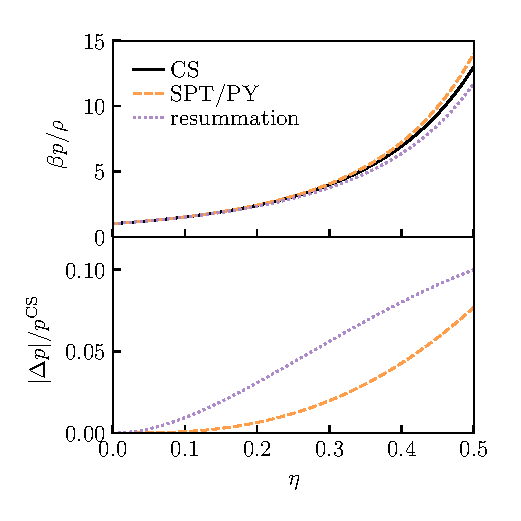
\includegraphics[width=0.9\linewidth,outer]{resummation-pressure}
  \caption[Accuracy of equation of state from partially resumming the virial series]{
    Equations of state for the single-component hard sphere liquid: Carnahan-Starling (CS), the scaled particle/Percus Yevick (SPT/PY) and the equation obtained from resumming terms in the virial series where there is a commong point of intersection.
    Top panel: pressure equations of state.
  Bottom panel: errors in the SPT/PY and resummation pressures are comparable across the whole liquid regime, taking the CS equation as the quasi-exact result.}
  \label{fig:resummation-pressure}
\end{SCfigure}

For single-component hard spheres the pressure obtained from the resummation in the previous section yields
\begin{equation}
  \frac{\beta p}{\rho} =
  \begin{cases}
    \frac{1}{1-\eta} & \; d=1 \\
    \frac{1}{(1-\eta)^2} & \; d=2 \\
    \frac{1 + \eta + (\frac{3\pi^2}{16} - 2) \eta^2}{(1-\eta)^3} & \; d=3.
  \end{cases}
\end{equation}
The resulting pressures for $d \le 2$ are identical to the scaled particle theory equations of state, where the first is the exact solution \eqref{eq:hard-rods-eos}.
For $d=3$ the resulting equation of state has a similar structure to the scaled particle theory solution (or equivalently the Percus-Yevick equation of state by the compressibility route) (SPT/PY) but it is slightly less accurate: at the freezing point $\eta_f \simeq 0.494$ the PY equation overestimates the pressure by $\sim7\%$ while for the above equation this is underestimated by $\sim11\%$, taking the Carnahan-Starling (CS) equation of state \cite{CarnahanJCP1969} as an estimate of the exact value.
The three equations of state mentioned are plotted together in Fig.\ \ref{fig:resummation-pressure} across the whole liquid regime in hard spheres.
While not exact, this shows that the morphometric contributions account for $\sim$90\% of the contributions to the equation of state which may suggest why morphological thermodynamics has been found to be highly accurate for descriptions of the hard sphere liquid \cite{RothPRL2006,LairdPRE2012,BlokhuisPRE2013,UrrutiaPRE2014,Hansen-GoosJCP2014,RobinsonPRL2019}.
This is discussed in more detail in the context of FMT in \cite{MarechalPRE2014}, and is partially attributable to cancellations of terms omitted from the resummation.

To account for the reduced accuracy of this equation of state for $d=3$ compared with PY, we observe that the PY hard sphere solution captures the third virial coefficient exactly, while this approach only provides a lower bound; the omitted configurations are known in the FMT literature as ``lost cases'' \cite{TarazonaPRE1997}.
A semi-empirical approach could reweight the final term in \eqref{eq:a3-d=3} to produce the third virial coefficient (if known), giving an equation of state for arbitrary mixtures of convex particles.
This reweighting is implicit in scaled particle theory and the Rosenfeld FMT functional \cite{TarazonaPRE1997,MarechalPRE2014}.

We see similar accuracy in the predicted surface tension at an infinite planar wall determined by $a_2$
\marginfootnote{This is true up to a normalisation constant, as $a_2$ conjugates with the intrinsic volume $V_2$ rather than the area $A = 2V_2$.
  The usual planar surface tension is thus obtained as $\gamma_\infty = a_2/2$.}.
The surface tension at an infinite planar wall is simply $a_2$ because it conjugates with the area.
In Ref.\ \cite{DavidchackMP2015} the results of extensive simulations measuring $a_2$ were parameterised by the following expression
\begin{equation}\label{eq:quasi-exact-surface-tension}
  %\begin{split}
  \beta a_2
  =
  \frac{1}{\pi \sigma^2} \left(
  \frac{\eta (2 + 3\eta - \frac{9}{5}\eta^2 - \frac{4}{5}\eta^3 - (5 \times 10^4) \eta^{20})}{(1 - \eta)^2}
  %% \right.
  %% \\
  %% &
  %% \left.
  %% \vphantom{\frac{1}{1}}
  - \ln{(1 - \eta)}
  \right),
  %\end{split}
\end{equation}
which we use to gauge the accuracy of predicted surface tensions.
We also compare the values of $a_2$ predicted by other morphometric theories of Ref.\ \cite{Hansen-GoosJPCM2006} (SPT/CS) and Ref.\ \cite{RobinsonPRE2019} (virial/CS).
The surface tensions are plotted in Fig.\ \ref{fig:resummation-a2}; the accuracy of the new result is comparable to SPT/PY in the liquid regime with the maximum error reaching $\sim12\%$.
Unsurprisingly, the other morphometric theories feature more accurate surface tensions; this is likely because they were constructed to satisfy thermodynamic relations which improves their accuracy.
%By contrast, the resummation route was not constructed for accuracy nor to satisfy thermodynamic relations.
Curiously, the error in the new theory scales almost identically to virial/CS theory at small $\eta$ even though the sign is different; all of the previous morphometric theories overestimate the surface tension, whereas the resummation route underestimates it.

\begin{SCfigure}
  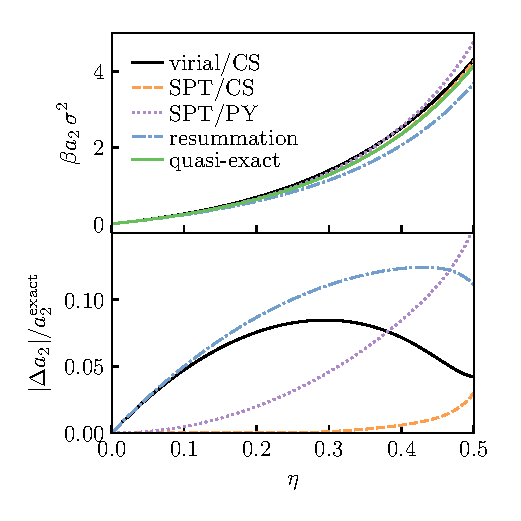
\includegraphics[width=0.9\linewidth,outer]{resummation-a2}
  \caption[Accuracy of surface tension from partially resumming the virial series]{
    Comparison of surface tensions for different morphometric theories.
  using the highly accurate result \eqref{eq:quasi-exact-surface-tension} from Ref.\ \cite{DavidchackMP2015} valid until $\eta \sim 0.5$.}
  \label{fig:resummation-a2}
\end{SCfigure}

%% \subsection{Beyond convex geometries and the choice of dividing surface}
%% \label{sec:general-geometries}

%% \begin{figure*}
%%   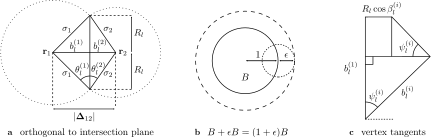
\includegraphics[width=0.65\linewidth,outer]{minkowski_addition}
%%   \caption{A dimer geometry considered in pair correlations in a fluid of $B$ particles showing (a) solute of two spheres $A$ generating an excluded volume $A \minkplus B$ and (b) the effective connected solute $A \minkplus B \minkminus B$.
%%   The exluded volume in each case is identical i.e.\ $A \minkplus B \minkminus B \minkplus B = A \minkplus B$.}
%%   \label{fig:minkowski_addition}
%% \end{figure*}

%% Until now we have focused on convex bodies, but we will now argue that the results apply for more general bodies.
%% In particular, for many-body correlations the ``solute'' consists of the disjoint union of particles see e.g.\ Fig.\ \ref{fig:system}.
%% We will determine necessary conditions for validity of the morphometric approach in in general solutes by examining the exact morphometric contributions described in previous sections.
%% A related problem is thermodynamic consistency for different choices of dividing surfaces in \eqref{eq:surface-tension}, which we will address in parallel.

%% Based on the exact results there are two ways the approach could fail:
%% \begin{enumerate}
%% \item For geometries where the integral geometric formula are invalid, e.g.\ the kinematic integrals, for non-convex geometries kinematic formula, and
%% \item Where the interaction with the solute cannot be reduced to the Euler characteristic, i.e.\ \eqref{eq:interactions-euler-equivalence}.
%% \end{enumerate}
%% As there are exact morphometric contributions to the free energy, a good approximation scheme should contain these; conversely, where these contributions are not captured provides necessary conditions for the scheme's validity.
%% We will address both potential failures in turn.

%% We used the kinematic integral \eqref{eq:binomial-kinematic-equation}, and its iterated form \eqref{eq:multinomial-kinematic-equation}, with convex bodies but it is valid for many more physically relevant geometries.
%% They can be extended \cite{Klain1997} to so-called \emph{polyconvex} bodies (also known as the convex ring), meaning any body formed by the countable union of convex objects.
%% This latter category covers most physically meaningful geometries, omitting pathological cases where size measures lose their meaning creating paradoxes \cite{BanachFM1924}.
%% The argument from Hadwiger's theorem similarly extends to polyconvex bodies.

%% Though the integral theorems hold for geometries of relevant physical interest, the equivalence between interaction and geometry \eqref{eq:interactions-euler-equivalence} may not.
%% We will consider two examples below in order to extend the geometric formalism to cases of physical interest.

%% First, consider the geometry formed by creating an infinitesimally small cavity inside a convex object.
%% Its Euler characteristic will deviate by $\pm 1$ (with sign dependent on dimension), however the interactions are unchanged because the cavity is not large enough to contain a finite-sized object.
%% In this case \eqref{eq:interactions-euler-equivalence} holds so long as the original convex geometry is used in place of the `true' body with the cavity.
%% %Going a step further, for finite-sized cavities able to contain a solvent particle, the cavity will be dynamically inaccessible to solvent particles (unless initially prepared inside) so the whole body can be treated as if it were solid, i.e.\ the interior of $\partial B$.

%% Next, we consider a geometry more typical of correlations in liquids: a dimer formed by two unit balls a distance $r$ apart i.e.\
%% \begin{equation*}
%%   A(r) = B^d \cup \mathcal{T}(r) B^d,
%% \end{equation*}
%% sketched in Fig.\ \ref{fig:minkowski_addition}.
%% This geometry is non-convex, and for $r > 1$ it is not even simply connected.
%% For interactions with a convex solvent particle $B$ we have possible Euler characteristics of intersection $\chi(A \cap B) \in \{0, 1, 2\}$ whereas $e^{-\beta u(A, B)} \in \{0, 1\}$, so it is not possible to establish an exact correspondence between the two.
%% We can proceed by determining an effective geometry where this relation does hold.
%% The exact result \eqref{eq:exact-mayer-exclusion} can be written
%% \begin{equation}
%%   \begin{split}
%%     e^{-\beta u(A, \mathcal{T} B)} - 1
%%     &= -\chi((A \minkplus B) \cap \{\vec{r}\}) \\
%%     &= -\chi((A \minkplus B \minkminus B) \cap B),
%%   \end{split}
%% \end{equation}
%% with the last line valid so long as $A \minkplus B \minkminus B = \{\vec{c} \, | \, (\vec{c} \minkplus B) \subseteq A \minkplus B\}$ is simply connected, otherwise the Euler characteristic of the intersecting geometry can be greater than one $\chi((A \minkplus B \minkminus B) \cap B) > 1$.
%% The effective geometry $A \minkplus B \minkminus B$ recovers the correspondence between interaction and geometry \eqref{eq:interactions-euler-equivalence}.
%% Addition (dilation) and subtraction (erosion) operations are not inverse operations so $A \minkplus B \minkminus B \ne A$, however $A \minkplus B \minkminus B \minkplus B = A \minkplus B$ so $A \minkplus B \minkminus B$ acts as an effective generator of the exclusion region.
%% The effective geometry for the previous example, a nearly convex body with an infinitesimal cavity, recovers the convex object.

%% Related to the above discussion is the effect of the choice of dividing surface on the decomposition of surface and volume terms in \eqref{eq:surface-tension}.
%% The thermodynamics should not depend on the choice of boundary, i.e.\ we can define a functional working with the parallel surface
%% \begin{equation*}
%%   \Delta \Omega'[A \minkplus \epsilon B]
%%   =
%%   \sum_{k=0}^d a_k' V_k(A \minkplus \epsilon B)
%% \end{equation*}
%% but thermodynamic consistency requires
%% \begin{equation*}
%%   \Delta \Omega[A] =
%%   \Delta \Omega'[A \minkplus \epsilon B].
%% \end{equation*}
%% A controlled expansion of the solvation energy which allows for different choices of dividing surface must be invariant to the particular choice.
%% The transformation between the coefficients $\{a_k\}$ and $\{a'_k\}$, which we give explicitly in Appendix~\ref{appendix:parallel-surfaces}, are straightforward which is a particular strength of using the morphometric \emph{ansatz}.
%% When this transformation fails leading to inconsistent thermodynamics, we know the theory has failed.
%% We find a necessary condition for the theory's validity is thus that $\chi(A \minkplus B^d \minkminus B^d) = \chi(A \minkplus B^d)$.

%% The boundary of the effective volume $\partial(A \minkplus B \minkminus B)$ is commonly called the \emph{molecular surface} \cite{?}, while the boundary of the excluded volume $\partial(A \minkminus B)$ is referred to as the \emph{solvent accessible surface}.
%% There is also an infinite family of equivalent parallel surfaces in between i.e.\ $\partial(A \minkplus B \minkminus \epsilon B)$ for $\epsilon \in [0, 1]$ but the two extremes are the most natural choices.
%% When the boundary of the effective geometry (molecular surface) self-intersects, we expect the theory to break down.
%% In the previous example this occurs at $r = 2\sqrt{3}$ for spherical solvent particles $B = B^d$ \cite{OettelEL2009}.
%% At this point, descriptions with different choices of boundary become inconsistent.
%% Consider the Euler characteristic of the effective body (molecular surface)
%% \begin{equation}
%%   \chi(A \minkplus B^d \minkminus B^d)
%%   =
%%   \begin{cases}
%%     1 & r < 2\sqrt{3} \\
%%     2 & r > 2\sqrt{3}
%%   \end{cases}
%% \end{equation}
%% whilst for the parallel volume (solvent accessible surface)
%% \begin{equation}
%%   \chi(A \minkplus B^d)
%%   =
%%   \begin{cases}
%%     1 & r < 2 \\
%%     2 & r > 2
%%   \end{cases}
%% \end{equation}

\section{Discussion}

%We have derived the morphometric solvation free energy for mixtures of hard convex particles from first-principles using the virial series.

While the morphometric theory we have derived from the virial series is less accurate than theories obtained from other routes. 
Specifically, in $d=3$ the pressure and surface tension is comparable in accuracy to the classic SPT/PY route and in $d=2$ the two approaches are equivalent.
\todo{Check that surface tension in $d=2$ is the same as SPT.}
However, the usefulness of the new route is extends beyond mere accuracy; the free energy we have identified emerges \emph{rigorously} as a contribution from the virial series.
The fact that this exact contribution is still reasonably accurate suggests that the corrections to it are small, providing further justification of the morphometric approach.
This means we could write the insertion cost for a solute $K$ as the \emph{exact} decomposition
\begin{equation}\label{eq:exact-morph-decomposition}
  \Delta \Omega[K]
  =
  \sum_{k=0}^d a_k V_k(K)
  + \Delta \Omega_\mathrm{extra}[K]
\end{equation}
with coefficients $a_k$ as previously calculated, and $\Delta \Omega_\mathrm{extra}$ contains the remaining contributions.
Notably the exponentially damped oscillations occuring in pair correlations at asymptotically large separations must be contained within $\Delta \Omega_\mathrm{extra}$.
The insertion cost is known to contain singularities \cite{ReissJCP1959} so it is unlikely that $\Delta \Omega_\mathrm{extra}$ possesses a simple analytic form.
It is possible that additional exact morphometric contributions exist, and they would be contained in $\Delta \Omega_\mathrm{extra}$ also.

Furthermore, the formal derivation we have followed naturally leads to explicit expressions for $\Delta \Omega_\mathrm{extra}$.
The next leading contribution from the virial series would be:
\begin{equation}
  \Delta \Omega_\mathrm{extra}[K]
  =
  \frac{\rho^2}{2}
  \sum_{s_1=1}^m \sum_{s_2=1}^m
  x_{s_1} x_{s_2}
  \left(
  \int_{G_d^2} \chi(K \cap g_1 K_{s_1}) \chi(K \cap g_2 K_{s_2}) \chi(g_1 K_{s_1} \cap g_2 K_{s_2}) dg_1 dg_2
  - \Lambda_{s_1,s_2} \right)
  + \mathcal{O}(\rho^3),
\end{equation}
which involves a \emph{ring integral}.
These integrals can be calculated straightforwardly in hard spheres \cite{MontrollJCP1941}, or using the Radon transform for convex geometries of arbitrary shapes \cite{WertheimMP1994,WertheimMP1996,WertheimMP1996a}.
Corrections could be systematically included by further resummations over topologically identical integrations, with ring integrals as the leading order terms.
The integral corrections are discussed in Ref.\ \cite{MarechalPRE2014} in the context of free energy functionals for inhomogeneous liquids; our system is effectively homogeneous so we expect it to be easier to construct a theory with higher-order terms.

The form of the exact contribution is instructive in how it applies to mixtures.
It is argued in Ref.\ \cite{KodamaJCP2011} that for an $m$-component mixture the appropriate morphometric form reads
\begin{equation}\label{eq:morphometric-approach-mixtures}
  \Delta \Omega
  =
  \sum_{i=1}^m
  a_3^{(i)} V_i
  + a_2^{(i)} A_i
  + a_1^{(i)} C_i
  + a_0^{(i)} X_i
\end{equation}
where the coefficients $a_k^{(i)}$ now depend on the specific interactions with each species and their composition, and $\{V_i, A_i, C_i, X_i\}$ are geometric measures on some composite body of the solute with solvent particles of species $i$, e.g.\ their specific exluded volume.
By contrast, our exact morphometric contribution does not involve different intrinsic volumes for the different cross-species interactions, suggesting \eqref{eq:morphometric-approach} is a general enough \emph{ansatz} and the extension for mixtures \eqref{eq:morphometric-approach-mixtures} proposed in Ref.\ \cite{KodamaJCP2011} may be unnecessary.

In addition to the accuracy of the exact contribution, we can argue against the alternative morphometric form for mixtures \eqref{eq:morphometric-approach-mixtures} by considering the polydisperse mixture limit.
The alternative form contains $4m$ parameters which becomes underconstrained in the polydisperse limit $m \to \infty$, so it is unlikely that the coefficients $a_k^{(i)}$ can be totally independent.
More precisely, thermodynamic consistency of the (osmotic) pressure requires
\begin{equation}\label{eq:osmotic-consistency-1}
  \begin{split}
    \beta p
    &=
    \rho - \beta f^\mathrm{ex}
    + \rho \left( \frac{\partial \beta f^\mathrm{ex}}{\partial \rho} \right)_{V,T}
    \\
    &=
    \rho - \beta f^\mathrm{ex}
    + \rho \sum_{i=1}^m
    x_i \left( \frac{\partial \beta f^\mathrm{ex}}{\partial x_i} \right)_{V,T}
  \end{split}
\end{equation}
where $f^\mathrm{ex} = F^\mathrm{ex}/V$ is the (excess) free energy density.
The latter line, valid in the case of mixtures, becomes poorly defined in the polydisperse limit $m \to \infty$ with $x_i \to 0$.
To remain well-defined for polydisperse systems the composition dependence of the free energy should reduce to a (finite) set of \emph{weighted densities} \cite{GualtieriJCP1982, WarrenPRL1998, SollichPRL1998, SollichAiCP2001}.
This is the case for our virial-derived approach where the density dependence enters through scaled particle variables $\{\xi_k\}$, so \eqref{eq:osmotic-consistency-1} becomes
\begin{equation}\label{eq:osmotic-consistency-2}
  \beta p
  =
  \rho - \beta f^\mathrm{ex}
  + \sum_k
  \xi_k \left( \frac{\partial \beta f^\mathrm{ex}}{\partial \xi_k} \right)_{V,T}.
\end{equation}
To demonstrate that our form works for both discrete and continuous (polydisperse) mixtures, we rewrite the geometric parameters \eqref{eq:spt-variables} in the more general form
\begin{equation}
  \xi_k
  =
  \rho \int \widetilde{V}_k(K_s) d\mu(s),
\end{equation}
introducing the probability measure $\mu(s)$ for the molarities of particle species/shapes such that $\int d\mu(s) = 1$.
This reduces to the previous form for discrete mixtures if we set $\mu(s)$ to the counting measure, however in integral form we are free to extend the calculation to continuous mixtures.

As an example we consider a polydisperse mixture of particles of reference shape $K$ with uniformly distributed sizes $s \in [s_0, s_1]$ giving $V_k(K_s) = V_k(s K) = s^k V_k(K)$, then
\begin{equation}
  \begin{split}
    \xi_k
    &=
    \rho \widetilde{V}_k(K) \int_{s_0}^{s_1} s^k ds
    \\ &=
    \rho \widetilde{V}_k(K) \left(\frac{s_1^{k+1} - s_0^{k+1}}{k+1}\right).
  \end{split}
\end{equation}
Inserting this reweighted volume into the explicit expressions given in the appendix yields new thermodynamic coefficients for uniformly distributed polydisperse mixtures.
The composition dependence enters only through moments of the size distribution guaranteeing a well-defined free energy, detailed discussion of which can be found in Refs.\ \cite{GualtieriJCP1982,WarrenPRL1998,SollichPRL1998,SollichAiCP2001}.

\section{Summary}

We have derived an exact morphometric contribution for a general class of hard particle liquids by resumming terms in the virial series.
Previous studies have primarily used FMT to develop morphometric theories, so we have successfully developed an independent justification for the morphometric approach as the leading term in a controlled expansion.
The exact result applies for mixtures of hard convex particles in an isotropic phase.

%This result is not that surprising as the morphometric approach can be obtained as a limit case of FMT \cite{Hansen-GoosJPCM2006}, which itself can be formulated as the resummation of the same terms in the virial expansion \cite{LeithallPRE2011,KordenPRE2012,MarechalPRE2014}.

In hard spheres the exact contribution features similar accuracy as scaled particle theory, so it captures most contributions to the bulk free energy and seems to be why the approach has been successful.
Though as noted in Ref.\ \cite{MarechalPRE2014} this is partially due to a cancellation in the omitted terms of the virial expansion, so it may still desirable to improve the morphometric approach by inclusion of additional terms.
The exact morphometric contribution provides a suitable starting point for including additional terms to improve accuracy.

%\appendix*

\section{Explicit morphometric contributions in the virial expansion}
%\label{appendix:lambda}

Here we explicitly evaluate the contributions in the virial expansion from configurations sharing a common point of intersection via \eqref{eq:little-lambda}.

For $d=1$ the index runs over $k \in \{0,1\}$, giving condition on the summation indices $N_0 = k$ and $N_1 = n - N_0$ leading to a single term for each value of $k$:
\begin{subequations}
  \label{eq:little-lambda-d=1}
  \begin{align}
    \lambda_0^{(n)} &= \xi_1^n
    \\
    \lambda_1^{(n)} &= n \xi_0 \xi_1^{n-1}.
  \end{align}
\end{subequations}
For $d=2$ we have $k \in \{0,1,2\}$, with summation conditions $2N_0 + N_1 = k$ and $N_2 = n - N_1 - N_0$ giving:
\begin{subequations}
  \label{eq:little-lambda-d=2}
  \begin{align}
    \lambda_0^{(n)} &= \xi_2^n
    \\
    \lambda_1^{(n)} &= n \xi_1 \xi_2^{n-1}
    \\
    \lambda_2^{(n)} &=
    n \xi_0 \xi_2^{n-1}
    + \frac{n(n-1)}{2} \xi_1^2 \xi_2^{n-2}.
  \end{align}
\end{subequations}
Finally, for $d=3$ we have $k \in \{0,1,2,3\}$, with summation conditions $3N_0 + 2N_1 + N_2 = k$ and $N_3 = n - N_2 - N_1 - N_0$ giving:
\begin{subequations}
  \label{eq:little-lambda-d=3}
  \begin{align}
    \lambda_0^{(n)} &= \xi_3^n
    \\
    \lambda_1^{(n)} &= n \xi_2 \xi_3^{n-1}
    \\
    \lambda_2^{(n)} &=
    n \xi_1 \xi_3^{n-1}
    + \frac{n(n-1)}{2} \xi_2^2 \xi_3^{n-2}
    \\
    \lambda_3^{(n)} &=
    n \xi_0 \xi_3^{n-1}
    + n(n-1) \xi_1 \xi_2 \xi_3^{n-2}
    \nonumber \\ & \qquad
    + \frac{n(n-1)(n-2)}{6} \xi_2^3 \xi_3^{n-3}.
  \end{align}
\end{subequations}

We will now resum $\lambda_k^{(n)}$ over $n$ in order to determine the values of $a_k$ for $d \le 3$.
For $d=1$ we insert \eqref{eq:little-lambda-d=1} into \eqref{eq:final-a-coefficient}:
\begin{subequations}
  \begin{align}
    \beta a_0
    &= - \ln{(1 - \eta)},
    \\
    \beta p =
    \beta a_1 &=
    \frac{2 \xi_0}{1-\eta},
  \end{align}
\end{subequations}
with $\xi_0 = \rho / 2$ giving the exact result for hard rods \eqref{eq:hard-rods-morphometric} and \eqref{eq:hard-rods-eos}.
For $d=2$ we insert \eqref{eq:little-lambda-d=2} into \eqref{eq:final-a-coefficient}:
\begin{subequations}
  \begin{align}
    \beta a_0 &= -\ln{(1 - \eta)},
    \\
    \beta a_1 &= \frac{2 \xi_1}{1-\eta},
    \\
    \beta p =
    \beta a_2 &=
    2\pi \left(
    \frac{\xi_0}{1-\eta}
    + \frac{\xi_1^2}{2(1-\eta)^2}
    \right).
  \end{align}
\end{subequations}
Note: for hard discs of diameter $\sigma$ we obtain $V_1 = \pi \sigma / 2$ so $\xi_0 = \rho / (2\pi)$ and $\xi_1 = \rho \sigma / 2$ for the single-component fluid.
Finally, for $d=3$ we insert \eqref{eq:little-lambda-d=3} into \eqref{eq:final-a-coefficient}:
\begin{subequations}
  \begin{align}
    \beta a_0 &= -\ln{(1 - \eta)},
    \\
    \beta a_1 &= \frac{2 \xi_2}{1-\eta},
    \\
    \beta a_2 &=
    2 \pi
    \left(
    \frac{\xi_1}{1-\eta}
    + \frac{\xi_2^2}{2(1-\eta)^2}
    \right),
    \\
    \beta p =
    \beta a_3 &=
    8 \pi\left(
    \frac{\xi_0}{1-\eta}
    + \frac{\xi_1 \xi_2}{(1-\eta)^2}
    + \frac{\xi_2^3}{3 (1-\eta)^3}
    \right).
    \label{eq:a3-d=3}
  \end{align}
\end{subequations}
Note: for hard spheres of diameter $\sigma$ we obtain $V_1 = 2\sigma$ and $V_2 = \pi \sigma^2 / 2$ so $\xi_0 = \rho / (8\pi)$, $\xi_1 = \rho \sigma / (2\pi)$ and $\xi_2 = \rho \pi \sigma^2 / 8$ for the single-component fluid.
In the above steps we have used the fact that $\xi_d = \eta$ to simplify the resulting expressions.

\ifdefined\includebibliography
  \printbibliography
\fi

\end{document}

%TC: macro \marginfootnote [other]
%TC: envir SCfigure [] other
%TC: macrocount beginSCfigure [figure]
\documentclass[11pt,twoside]{report}
\usepackage{preamble}
\setcounter{chapter}{5}
\graphicspath{{../img/}}
\def\includebibliography{}

\begin{document}
\chapter{Nucleation kinetics in simple drying aerosols}
\epigraph{Remove the plastic.}{Sears\textsuperscript{\textregistered} cross-trainer manual.}
\label{chapter:aerosols}

In previous chapters we focused on modelling hard spheres at high densities, with a particular focus on supercooled liquids and glasses.
As we mentioned in the introduction, another central topic of the high density liquid is the process of nucleation by which the liquid becomes a crystal.
This chapter addresses nucleation within the context of drying aerosol droplets, with applications to climate modelling and industrial spray drying.
The chemistry involved in aerosols makes this system much more complicated than can be captured with a simple hard sphere interaction, so our microscopic morphometric formalism will not work here at present.
Instead, we start from the mesoscale limit where the droplet can be treated as a continuum.
%% At present real systems are too complex to be treated from first principles, so we will employ phenomenological fits to available data assuming classical nucleation theory.
%% We hope one day theory will allow a connection between microscopic and mesoscopic approaches, paving the way to a properly first-principles treatment of real systems.

This work was undertaken in collaboration with members of the Reid group in the School of Chemistry at the University of Bristol.
In particular, the experiments were carried out by Flo Gregson.
My contribution to this work was through theory and numerical modelling to better understand the experimental data.
Consequently, while I will describe the experiments the focus of the chapter will be theoretical.
Some of this work has already been published in Ref.\ \cite{GregsonJPCB2019}, and we hope to publish the remainder as Refs.\ \cite{RobinsonTBD2019,GregsonTBD2019} later this year.

Finally, for the benefit of those working in the field of supercooled liquids and glasses who are reading this and wondering what this chapter has to do with the rest of the thesis, we put forward the following additional motivation: in order to finally solve the glass transition, we must address the looming climate crisis to keep glass researchers alive long enough to actually reach a consensus%
\marginfootnote{On second thought, I suppose another option would be: ``last statistical physicist alive gets to decide the nature of the glass transition''.}[-2cm].
As such, consider this chapter a small step in consensus building.

\section{Introduction}

The impact of atmospheric aerosols on the climate remains the leading single uncertainty in climate predictions \cite{BoucherIPCC2013,CarslawN2013,LeePNAS2016,RegayreACP2018}.
In particular, the radiative forcing caused by anthropogenic aerosols in clouds features large uncertainties due to the difficulty of direct measurement, and the large parameter spaces of theoretical models \cite{LeePNAS2016}.
Thus, the importance of improving models for atmospheric aerosols to better predict climate change and inform policy cannot be overstated.
In addition, atmospheric aerosols have potential applications in geoengineering \cite{PringleACP2012}.

Notably, radiative forcing of atmospheric aerosols is stongly influenced by their optical properties \cite{HodasACP2015,CotterellACP2017}.
The solute concentration and physical state (i.e.\ whether it is crystalline or amorphous) can thus have a dramatic effect on climate predictions.
Central to this is the nucleation and drying kinetics of atmospheric droplets.
Where aerosols are included in climate models the focus is typically on sulphates \cite{MannACP2014,ZhuNC2019}.
However, sea salt aerosols (e.g.\ those containing \ce{NaCl}), deposited into the atmosphere through natural processes, are more prevalent in the atmosphere than sulphates making up the second largest component of atmospheric aerosols by mass \cite{KeeneJAS1998}; a major component of aged \ce{NaCl} aerosols is sodium nitrate (\ce{NaNO3}) formed through reactions with nitrogen oxides \cite{TolockaJPCA2004}, a significant industrial emission.
Subsequent reactions form secondary organic aerosols which further impact the climate \cite{ScottACP2014,PoschlCR2015} and are associated with adverse health effects \cite{PoschlCR2015}.
Given their abundance and relative simplicity we focus on \ce{NaCl} and \ce{NaNO3} aerosol droplets.

Understanding the droplet drying and crystallisation process is also important for industrial applications, most notably in spray-drying.
The goal in these applications is to control the distribution of sizes, morphology and phase of the final droplets, which are very sensitive to processing conditions such as solvent \cite{CarverIECR2012,LintingreSM2016}, temperature \cite{IveyAST2018,YouDT2014,LinPT2015}, pH \cite{YuJPS2002,DubbiniIJP2014} and additional co-excipients \cite{ZhongAP2018,NandiyantoAPT2011,LyuJCG2017}.
Tailoring crystallisation is particularly important because crystal and amorphous states have fundamentally different properties: crystalline droplets are typically more stable, suitable for e.g.\ product storage \cite{VehringJAS2007,CostantinoJPS1998}, whereas amorphous droplets are more soluble which is desirable for e.g.\ drug delivery \cite{AmstadJPCB2016,BroughIJP2013}.
Our investigation of crystal nucleation rates can be inverted to design spray-drying conditions to achieve a desired final state.

In this chapter we will investigate drying and crystal nucleation of free aerosol droplets, by combining experiments and a numerical model of free aerosol droplets.
The experiments are described in section \ref{sec:experiments}, and we report matching them to a diffusional model of droplet evolution in section \ref{sec:evolution}.
We find that classical nucleation theory accurately predicts the crystallisation times for \ce{NaCl} aerosols, but not for \ce{NaNO3}, in section \ref{sec:nucleation}.
For \ce{NaNO3} we report nucleation rates with non-monotonic behaviour with increasing solute concentration.

\section{Experiments}
\label{sec:experiments}

The kinetics of drying \ce{NaCl} and \ce{NaNO3} droplets was measured using the Comparative-Kinetics Electrodynamic Balance (CK-EDB).
In all experiments HPLC-grade water, BioXtra $\ge 99.5\%$ \ce{NaCl} (Sigma-Aldrich) and analytic grade \ce{NaNO3} (Fisher-Scientific) were used.
The CK-EDB instrument has been detailed in previous work \cite{DaviesAST2012} so we will only describe it briefly here.
Droplets of known concentration are produced by a droplet-on-demand generator (MicroFab) and injected into the CK-EDB instrument.
Upon generation the droplets are charged ($<\SI{10}{\femto\coulomb}$ through e.g.\ an ionic imbalance) with an induction electrode such that they become trapped within the centre of the electrodynamic field, produced by the application of an AC field between two sets of concentric cylindrical electrodes.
An additional DC field is applied to the lower set of electrodes to counteract gravity and drag forces acting on the droplet.
A circulating current of ethylene glycol coolant across the electrodes controls the chamber temperature $T_{\infty}$ in the range 273--\SI{323}{\kelvin}.

To determine the size and physical state of the droplet, it is illuminated with a \SI{532}{\nano\metre} continuous-wave laser.
The resulting scattering pattern is recorded by a CCD camera placed at \SI{45}{\degree} to the beam over an angular range of $\SI{\sim24}{\degree}$.
For isotropic droplets in a liquid or dried amorphous state the droplet radius $R$ determines the angular separation between the fringes in the pattern $\Delta \theta$.
Assuming the geometric optics approximation of Mie theory, this relationship is given by
\begin{equation*}
  R
  =
  \frac{\lambda}{\Delta \theta} \left(
  \cos{\left(\frac{\theta}{2}\right)}
  + \frac{n \sin{\left(\frac{\theta}{2}\right)}}{\sqrt{1 + n^2 - 2n \cos{\left(\frac{\theta}{2}\right)}}}
  \right)^{-1}
\end{equation*}
where $\lambda$ is the laser wavelength, $\theta$ is the central viewing angle and $n$ is the droplet refractive index.
This approximation scheme determines the droplet radius within an accuracy of $\SI{\pm100}{\nano\metre}$.
This method fails when crystallisation occurs breaking isotropy and the scattering pattern dramatically changes; this feature allows the time of crystallisation to be determined to within $\SI{\sim10}{\milli\second}$.
Nucleation and growth occur on such a short time scale that it is not possible to obtain information from the experiments on where inside the droplet this occurs or how many initial nucleation sites there were; we can only determine that the droplet has nucleated crystals.

The instrument features two gas flows for wet and dry nitrogen applied to the droplet at a rate of \SI{0.03}{\metre\per\second}.
Controlling the ratio of these two flows through a mass-flow controller (MKS instruments) sets the relative humidity (RH) inside the CK-EDB chamber.
Liquid aqueous \ce{NaCl} and aqueous \ce{NaNO3} droplets (20\% solute concentration by weight) were evaporated into dry conditions at \SI{20}{\celsius}.
Crystallisation of multiple \ce{NaCl} droplets occurred reproducibly \SI{1}{\second} after droplet generation \cite{GregsonJPCB2019}, whereas \ce{NaNO3} droplets showed stochastic behaviour with a fraction of droplets not crystallising over the timescale of the experiment (droplets were typically trapped for \SI{10}{\second}).
The stochastic behaviour persists when the experiment was repeated for the \emph{same} \ce{NaNO3} droplet over a cycle of repeatedly lowering and raising the RH (described in more detail in Ref.\ \cite{GregsonTBD2019}), ruling out impurity-driven heterogeneous nucleation.

\begin{SCfigure}
  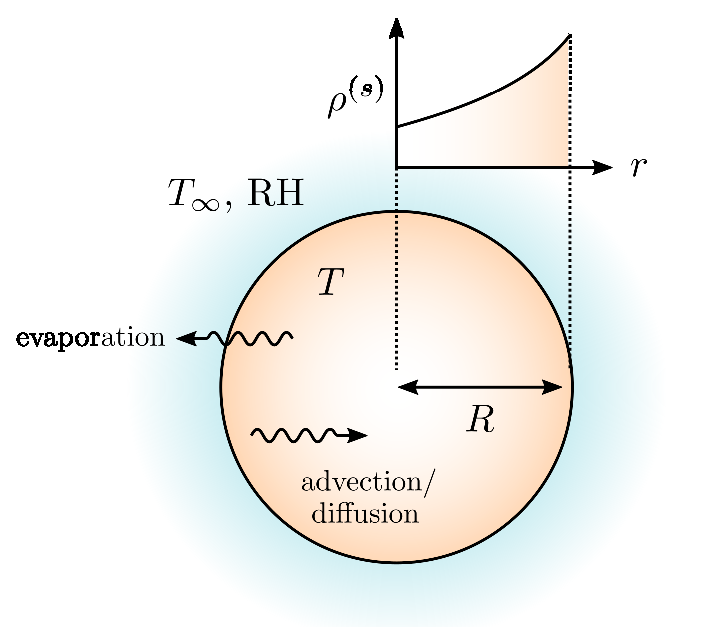
\includegraphics[width=0.75\linewidth,outer]{aerosol-droplet}
  \caption[Model drying aerosol droplet]{
    A drying droplet solution of radius $r=R(t)$ surrounded by a gas of temperature $T_\infty$ and relative humidity RH.
    Evaporation of the solvent (water) causes the droplet to shrink and surface enrichment of solute concentration $\rho^{(s)}$ together with evaporative cooling $T < T_\infty$.}
  \label{fig:aerosol-droplet}
\end{SCfigure}

Follow up experiments by the Reid group placed the droplets inside a scanning electron microscope (SEM) for imaging.
These found that for \ce{NaCl} aerosols nucleation seems to occur at the boundary%
\marginfootnote{I am reversing chronology here: actually, we used our numerical model to predict this \emph{first}, which was then was confirmed by SEM images.}.
The experiments featuring slower evaporation tended to have more perfect crystals suggesting there were fewer nucleation sites, whereas the more rapidly evaporating droplets showed imperfections consistent with there being multiple nucleation sites at the boundary \cite{GregsonTBD2019}.
The SEM results for \ce{NaNO3} were inconclusive, although the resulting crystals were more spherical suggesting there were multiple nucleation sites which may be less strongly distributed at the boundary.

\section{Model for a drying droplet}
\label{sec:evolution}

\subsection{Overview and notation}

In order to obtain nucleation rates we require the time evolution of the droplet's concentration profile over its drying history, and a phenomenological model for nucleation rates based on concentration.
To determine the concentration profile trajectory for a drying droplet we have to consider the relative motion of solute and solvent species inside the droplet, of various species in the surrounding vapour phase, as well as the evaporation of solvent across the phase boundary.
Our approximations will reduce this to a moving boundary problem with solely diffusional mixing.

Prior to crystallisation a drying droplet will be approximately spherical, so we consider a phase boundary at radius $R(t)$ evolving in time $t$.
Writing the distance from the center of the droplet as $r$, the phase boundary separates the liquid phase inside $r \in [0, R(t))$ from the vapour phase outside $r \in (R(t), \infty]$.
The droplet is sketched in Fig.\ \ref{fig:aerosol-droplet}.
%In the experiments are performed in ambient conditions so the surrounding gas is strictly speaking a mixture, but to a reasonable approximation we can treat it as a single component.

We label the solute and (ambient) gas components as $s$ and $g$ respectively, and the evaporating solvent component as $f$ for \emph{fluid} as it exists in both the liquid and gas phases.
The density is $\rho = \sum_i \rho^{(i)}$ where the (mass) concentration of each component is $\rho^{(i)}$ for $i \in (f,s)$ in the droplet and $i \in (f,g)$ in the gas.
A useful auxillary variable is the mass fraction of each component, i.e.\
\begin{equation}\label{eq:mass-fraction}
  Y^{(i)} = \frac{\rho^{(i)}}{\rho}.
  %{\sum_j \rho^{(j)}}
  %{\rho^{(f)} + \rho^{(s)}}
  %\frac{\rho^{(i)}(\vec{r})}{\rho^{(f)}(\vec{r}) + \rho^{(s)}(\vec{r})}
  %\qquad i \in \{f, s\}.
\end{equation}
%with $j$ running over the components of the relevant phase.
%Clearly $Y^{(f)} = 1 - Y^{(s)}$
As both phases are binary mixtures%
\marginfootnote{This is not strictly true.
  The liquid phase is certainly a binary mixture of solvent and solute, however the vapour is composed of the evaporated solvent and a multicomponent ambient gas phase.
  However, we can treat the ambient gas as an effectively single-component system to a very good approximation.}[-1.5cm]
so we only need to solve for one component; we choose to solve for the solute mass fraction $Y^{(s)}$ in the droplet and the solvent mass fraction $Y^{(f)}$ in the surrounding vapour.

The thermal conductivity of liquids is generally much larger than the mass diffusivity, so to leading order we can treat temperature $T$ as homogeneous throughout the droplet.
This approximation neglects potential conduction forces driven by temperature gradients.
The droplet temperature will be smaller than the ambient temperature $T_\infty$ because vaporisation carries a latent heat
We will determine $T$ through the rate of vaporisation which will be moderate the vaporisation rate and enter into the nucleation calculations.
However, as a simplification we do not incorporate this temperature into the dynamics themselves through modified diffusion coefficients.

\subsection{Evolution of the concentration profile}

In the absence of any chemical reactions the continuity equation for each species component reads
\begin{equation}\label{eq:species-continuity}
  \frac{\partial \rho^{(i)}}{\partial t} +
  \vec{\nabla} \cdot (\rho^{(i)} \vec{v}^{(i)}) = 0
  \qquad i \in \{f,s\}
\end{equation}
where $\vec{v}^{(i)}$ is the velocity of species $i$, or in terms of relative flows
%% and the mass-averaged fluid velocity is
%% \begin{equation}
%%   \vec{v} = \sum_i Y^{(i)} \vec{v}^{(i)}
%% \end{equation}
%% We have
%% \begin{equation*}
%%   \frac{\partial \rho^{(i)}}{\partial t} +
%%   \vec{\nabla} \cdot (\rho^{(i)} \vec{v}) +
%%   \vec{\nabla} \cdot (\rho^{(i)} (\vec{v}^{(i)} - \vec{v})) = 0
%%   \qquad i \in \{f,s\}
%% \end{equation*}
%% and defining the relative mass flux as
%% \begin{equation}\label{eq:relative-mass-flux}
%%   \vec{j}^{(i)} = \rho^{(i)} (\vec{v}^{(i)} - \vec{v})
%%   \qquad i \in \{f,s\}
%% \end{equation}
%% gives
\begin{equation}\label{eq:species-continuity-relative}
  \frac{\partial \rho^{(i)}}{\partial t} +
  \vec{\nabla} \cdot (\rho^{(i)} \vec{v}) +
  \vec{\nabla} \cdot \vec{j}^{(i)} = 0
  \qquad i \in \{f,s\}
\end{equation}
where the mass-averaged fluid velocity is $\vec{v} = \sum_i Y^{(i)} \vec{v}^{(i)}$ and the relative mass flux is $\vec{j}^{(i)} = \rho^{(i)} (\vec{v}^{(i)} - \vec{v})$.
Any advective/convective flows will typically be contained in $\vec{v}$, while diffusive effects are captured by $\vec{j}^{(i)}$.

Volume additivity holds to a good approximation \cite{HandscombCES2009}, i.e.\ the density and concentrations are related by
\begin{equation}\label{eq:volume-additivity}
  %\begin{split}
  \frac{1}{\rho} =
  \frac{Y^{(s)}}{\rho_0^{(s)}} + \frac{Y^{(f)}}{\rho_0^{(f)}}
  %% \sum_{k \in \{f,s\}} \frac{Y^{(k)}}{\rho^{(j)}_0} \\
  %% &=
  %% \frac{Y^{(i)}}{\rho^{(i)}_0} +
  %% \frac{1 - Y^{(i)}}{\rho^{(j)}_0}
  %% \qquad i,j \in \{f,s\}, \; j \ne i.
  %\end{split}
\end{equation}
where $\rho_0^{(s)}$ and $\rho_0^{(f)}$ are the densities of the pure substances in the liquid phase; as no stable amorphous phases of \ce{NaCl} or \ce{NaNO3} are known we approximate $\rho_0^{(s)}$ by the density in the crystal phase.

By considering mass conservation one obtains
\begin{equation*}
  \vec{\nabla} \cdot \vec{v}
  =
  \frac{1}{\rho^2}
  \frac{\partial \rho}{\partial Y^{(s)}}
  \vec{\nabla} \cdot \vec{j}^{(s)}
\end{equation*}
so assuming volume additivity \eqref{eq:volume-additivity} we can define the mass difference parameter as
\begin{equation}\label{eq:lambda}
  \Lambda
  =
  \frac{1}{\rho^2} \frac{\partial \rho}{\partial Y^{(s)}} \\
  =
  \frac{1}{\rho^{(f)}_0} -
  \frac{1}{\rho^{(s)}_0}
\end{equation}
giving $\vec{v} = \Lambda \vec{j}^{(s)}$.
This simplifies the advective term in the continuity equation \eqref{eq:species-continuity-relative} leading to
\begin{equation}\label{eq:species-continuity-relative-without-advection}
  \frac{\partial \rho^{(s)}}{\partial t} +
  \vec{\nabla} \cdot \left(
  (1 + \Lambda \rho^{(s)}) \, \vec{j}^{(s)}
  \right) = 0.
\end{equation}
For the relative mass flux we assume Fick's law for diffusion
\begin{equation}\label{eq:ficks-law}
  \vec{j}^{(i)} = -D_\mathrm{eff} \rho \vec{\nabla} Y^{(i)},
\end{equation}
where $D_\mathrm{eff}$ is an effective \emph{binary} diffusion constant for the relative motion.
Inserting \eqref{eq:ficks-law} into \eqref{eq:species-continuity-relative-without-advection} and using the product rule, i.e.\
\begin{equation*}
  %% \begin{split}
  \vec{\nabla} \rho^{(s)}
  =
  %% \vec{\nabla} \left( \rho Y^{(s)} \right)
  %% &=
  %% \rho \vec{\nabla} Y^{(s)}
  %% + Y^{(s)} \vec{\nabla} \rho
  %% \\ &=
  %% \rho \vec{\nabla} Y^{(s)}
  %% + Y^{(s)} \frac{\partial \rho}{\partial Y^{(s)}} \vec{\nabla} Y^{(s)}
  %% \\ &=
  %% \rho \vec{\nabla} Y^{(s)}
  %% + \Lambda Y^{(s)} \rho^2 \vec{\nabla} Y^{(s)}
  %% \\ &=
  \left(
  1 +
  \Lambda \rho^{(s)}
  \right)
  \rho
  \vec{\nabla} Y^{(s)}.
  %% \end{split}
\end{equation*}
Finally, this gives the standard diffusion equation
\begin{equation}\label{eq:final-diffusion}
  \frac{\partial \rho^{(s)}}{\partial t}
  =
  \vec{\nabla} \cdot \left(
  D_\mathrm{eff} \vec{\nabla} \rho^{(s)}
  \right)
\end{equation}
where the advective forces have vanished providing a convenient form for numerical implementation.
By comparison, the mass fraction is widely used in the literature (e.g.\ Ref.\ \cite{HandscombCES2009}) which leads to separate advection and diffusion terms i.e.\
\begin{equation*}
  \rho \left(
  \frac{\partial Y^{(s)}}{\partial t} +
  \underbrace{\vec{v} \cdot \vec{\nabla} Y^{(s)}}_\textrm{advection}
  \right)
  -
  \underbrace{\vec{\nabla} \cdot (D_{\textrm{eff}} \rho \vec{\nabla} Y^{(s)})}_\textrm{diffusion}
  = 0.
\end{equation*}

Bulk viscosity measurements are unavailable at high densities because of the propensity for the salts to crystallise, so we extrapolate the available experimental data \cite{PowerCS2013,BaldelliAST2016} assuming the Arrhenius-like form
\begin{equation}\label{eq:vft-fit}
  \log{\eta}
  =
  \log{\left(\eta(\rho^{(s)} = 0)\right)}
  + \alpha \rho^{(s)}
\end{equation}
where $\alpha$ is a fitting parameter.
The fits are shown in Fig.\ \ref{fig:diffusion-fit}(a).
We model the diffusion constant by assuming the Stokes-Einstein form
\begin{equation}\label{eq:stokes-einstein}
  D_\mathrm{eff} = \frac{k_B T}{6 \pi \eta a},
\end{equation}
where $a$ is the Stokes radius and $\eta$ is the dynamic viscosity.
To determine $a$ we calibrated direct measurements of diffusion from molecular dynamics simulations for \ce{NaCl} \cite{LyubartsevJPC1996} and experiments for \ce{NaNO3} \cite{YehJCED1970} against the viscosity fits.
We obtain $a=\SI{0.169}{\nano\metre}$ for \ce{NaCl} and $a=\SI{0.167}{\nano\metre}$ for \ce{NaNO3}.
The resulting diffusion coefficients entering the droplet evolution equation are shown in Fig.\ \ref{fig:diffusion-fit}(b).

\begin{SCfigure}
  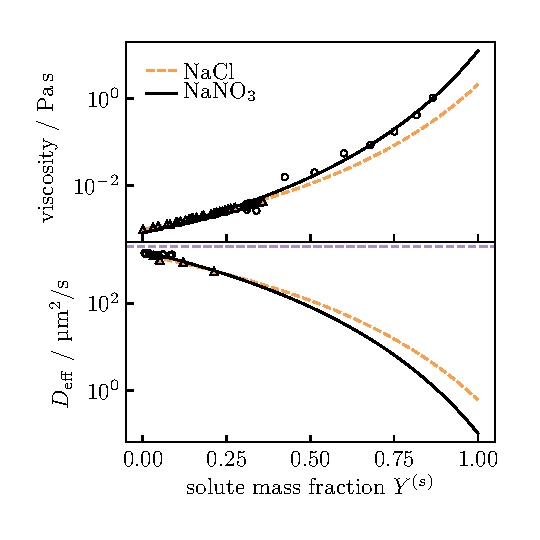
\includegraphics[width=0.9\linewidth,outer]{aerosol-diffusion-fit}
  \caption[Viscosity and diffusion coefficients of aqueous ionic solutions]{
    Numerical fits of binary diffusion coefficients for aqueous ionic solutions.
    a) fits of viscosity to an Arrhenius-like form \eqref{eq:vft-fit} to experimental values \cite{PowerCS2013,BaldelliAST2016}.
    b) diffusion coefficient from the viscosity fits assuming a Stokes-Einstein form \eqref{eq:stokes-einstein}, where the Stokes radius is obtained by calibration with direct measurements of diffusion at \SI{300}{\kelvin} for \ce{NaCl} \cite{LyubartsevJPC1996} and \SI{25}{\celsius} for \ce{NaNO3} \cite{YehJCED1970}.
    The dashed-purple horizontal line shows the diffusion constant of pure \ce{H2O} for reference, to be distinguished from the binary diffusion constants in the limit $Y^{(s)} \to 0$.}
  \label{fig:diffusion-fit}
\end{SCfigure}

We employ two simplifications in our calculations concerning the effects of droplet temperature.
First, our volume additivity assumption \eqref{eq:volume-additivity} makes the density temperature independent; this neglects conduction forces caused by temperature gradients and results in more heterogeneous droplets.
%In reality temperature gradients will be present in a drying droplet from evaporative cooling, so conductive forces will help keep the solution well-mixed; we will thus overestimate the inhomogeneities of the concentration profile.
Secondly, we approximate $T \sim T_\infty$ in the Stokes-Einstein relation \eqref{eq:stokes-einstein}
This approximation neglects evaporative cooling which would slow diffusion, so overestimates the diffusion constant and will result in more heterogeneous droplets.
It is unclear \emph{a priori} which of these opposing effects dominates.
Note: later we model the droplet temperature $T$ explicitly for treating solvent evaporation and nucleation rates, but we have not incorporated this temperature into the diffusion constant.

\subsection{Droplet boundary conditions}

Initially the droplets are prepared in equilibrium, so they are well-mixed solutions and we can assume a uniform initial concentration profile.
At $t=0$ the humidity is reduced leading to evaporation of the solvent.
The evaporation rate determines the boundary conditions for the diffusion equation \eqref{eq:final-diffusion}.

Integrating the species continuity equation \eqref{eq:species-continuity} gives the total mass flow into the droplet (of each species) as
\begin{equation}\label{eq:integral-continuity}
  \frac{d m^{(i)}}{dt} =
  \int_{V(t)} \frac{\partial \rho^{(i)}}{\partial t} \, d V +
  \int_{\partial V(t)} \rho^{(i)} \, \vec{v}_{\partial V(t)} \cdot d\vec{S}
%  \qquad i \in \{f,s\}
\end{equation}
where $V(t)$ is the volume of the droplet at time $t$ and $\vec{v}_{\partial V(t)}$ is the velocity of the boundary, and the vectorial surface element $d\vec{S}$ points in the direction of the outer normal vector.
We assume the solute does not leave the droplet, so all mass flow at the boundary must be due to the solvent.
Inserting the diffusion equation \eqref{eq:final-diffusion} into \eqref{eq:integral-continuity} and applying Stokes' theorem gives
\begin{equation}
  \frac{d m^{(s)}}{dt}
  =
  \int_{\partial V(t)}
  \Big(
  \rho^{(i)} \vec{v}_{\partial V(t)} +
  D_\mathrm{eff} \vec{\nabla} \rho^{(s)}
  \Big)
  \cdot d\vec{S}
  = 0.
\end{equation}
For spherical droplets this gives the boundary condition
%% \begin{equation}
%%   \frac{d m^{(s)}}{dt}
%%   =
%%   4 \pi R^2
%%   \rho^{(s)}(R) \left(
%%   \frac{dR}{dt}
%%   + \frac{D_\mathrm{eff}}{\rho^{(s)}} \frac{\partial \rho^{(s)}}{\partial r}
%%   \right)
%% \end{equation}
%% so
\begin{equation}
  \left. \frac{\partial \rho^{(s)}}{\partial r} \right|_{r=R(t)}
  =
  -
  \frac{\rho^{(s)}}{D_\mathrm{eff}(R)}
  \frac{dR}{dt}.
\end{equation}
Assuming volume additivity \eqref{eq:volume-additivity} we can determine the radial evolution from mass conservation as
\begin{equation}\label{eq:radial-evolution}
  \frac{dR}{dt}
  =
  \frac{\dot{m}}{4\pi R^2 \rho^{(f)}_0}
\end{equation}
so we need a model of the evaporation rate $\dot{m} := \tfrac{dm^{(f)}}{dt}$ to close this system of equations.

We now derive the classical result for quasistatic droplet vaporisation, loosely following the exposition of standard texts e.g.\ Refs.\ \cite{Slattery1999, Sirignano2010}.
Relaxation in the vapour phase occurs much faster than inside the liquid droplet, so we can assume that the flows in the vapour phase are quasi-steady.
The time-derivative in the continuity equations \eqref{eq:species-continuity} and \eqref{eq:species-continuity-relative} thus vanishes leaving
\begin{subequations}
  \begin{align}
    \vec{\nabla} \cdot (\rho \vec{v})
    &=
    0
    \\
    \vec{\nabla} \cdot (\rho^{(i)} \vec{v}^{(i)})
    =
    \vec{\nabla} \cdot (\rho^{(i)} \vec{v} + \vec{j}^{(i)})
    &=
    0
    \qquad i \in \{f,g\}
    %% \frac{1}{r^2} \frac{d}{dr} \left(
    %% r^2 \rho u Y_i - r^2 D_V \frac{d(\rho Y_i)}{dr}
    %% \right)
  \end{align}
\end{subequations}
with the total mass continuity equation obtained by summing over both species in \eqref{eq:species-continuity} and using $\sum_i \rho^{(i)} = \rho$.
Assuming spherical symmetry we find that total mass conservation obeys
\begin{equation}\label{eq:vapour-mass-conservation}
  r ^2 \rho v
  =
  \textrm{constant}
  =
  -\frac{\dot{m}}{4\pi}
\end{equation}
with radial speeds $v = |\vec{v}|$ and $v^{(i)} = |\vec{v}^{(i)}|$.
Similarly, for the evaporating component we obtain the ordinary differential equation
\begin{equation*}\label{eq:quasistatic-vapour-species-conservation}
  r^2 \rho v Y^{(f)} - r^2 \rho D_v \frac{d Y^{(f)}}{dr}
  =
  -\frac{\dot{m}}{4\pi}
\end{equation*}
where we assumed Fickian diffusion for the relative flux term with $D_v$ as the effective binary diffusion constant for the vapour.
Using total mass conservation \eqref{eq:vapour-mass-conservation} we can rewrite this as
\begin{equation}\label{eq:vapour-ode}
  \frac{d Q}{dr} (Y^{(f)} - 1)
  - \frac{d (Y^{(f)} - 1)}{dr}
  = 0
\end{equation}
with
\begin{equation}\label{eq:vapour-ode-integration-factor}
  Q(r)
  =
  \frac{\dot{m}}{4\pi}
  \int_r^\infty  \frac{1}{\rho D_v (r')^2} \, dr'.
\end{equation}
Upon integration%
\marginfootnote{One way of doing this is to multiply through by the integrating factor $e^{-Q(r)}$.}
we find
\begin{equation*}
  (Y^{(f)}(r) - 1) e^{-Q(r)}
  =
  \textrm{constant}.
\end{equation*}
or
\begin{equation*}
  \frac{1 - Y^{(f)}(R^+)}{\displaystyle{1 - \lim_{r \to \infty}} Y^{(f)}(r)}
  =
  1 + B
  =
  e^{Q(R)}
\end{equation*}
where the superscript in $Y^{(f)}(R^+)$ indicates the mass fraction of the solvent component is taken on the vapour side of the boundary and we have defined the \emph{Spalding number} as
\begin{equation}\label{eq:spalding-number}
  B
  =
  \frac{
    \displaystyle{\lim_{r \to \infty}} Y^{(f)}(r) - Y^{(f)}(R^+)
  }{
    1 - \displaystyle{\lim_{r \to \infty}} Y^{(f)}(r)
  }.
\end{equation}
Upon reinserting the definition of $Q(r)$ \eqref{eq:vapour-ode-integration-factor} and rearranging we obtain 
\begin{equation*}
  \frac{dm^{(f)}}{dt}
  =
  \frac{
    4\pi \ln{(1 + B)}
  }{
    \int_r^\infty  \frac{1}{\rho D_v (r')^2} \, dr'
  }.
\end{equation*}
If we take $\rho = \rho_v$ and $D_v$ as constants in the vapour phase, then we obtain the classical result for quasistatic vaporisation as \cite{Slattery1999,Sirignano2010}
\begin{equation}\label{eq:quasistatic-vaporisation}
  \frac{dm^{(f)}}{dt}
  =
  4\pi \rho_v D_v R \ln{(1 + B)}.
\end{equation}
Matching the partial pressures of the solvent on either side of the boundary through the Clausius-Clapeyron relation gives% the molar fraction
\begin{equation}\label{eq:molar-fraction}
  %X^{(f)}(R^+) =
  %a_w \frac{p_{eq}}{p}
  p_f(R^+)
  =
  p_f(R^-)
  \exp{\left( \frac{L}{R} \frac{T - T_\infty}{T T_\infty} \right)}
\end{equation}
where $p_f(R^\pm)$ are the partial pressures on either side of the surface which we can convert to mass fractions assuming Raoult's law in the gas phase combined with experimental fits of the solvent activity \cite{CleggJPCA1998}.
%The mass fraction $Y^{(f)}(R^+)$ can then be obtained from $X^{(f)}(R^+)$.
%% Neglecting the effects of radiative heat transfer, the steady state heat flux through the droplet boundary in the steady state is \cite{KulmalaJAS1992,RovelliJPCA2016}
%% \begin{equation}
%%   \dot{Q}
%%   =
%%   %Q_R
%%   - h \frac{dm^{(f)}}{dt} + 4\pi R K (T - T_\infty)
%% \end{equation}
%% %where $Q_R$ is the excess heat flux of radiation over absorption,
%% where $h_v$ is the vapour enthalpy of the evaporating solvent, and $K$ is the thermal conductivity of the gas phase.
Finally, assuming a steady state heat flux through the boundary, and neglecting the radiative heat transfer and the droplet heat capacity, gives the temperature difference between the droplet surface and the ambient temperature as \cite{KulmalaJAS1992,RovelliJPCA2016}
\begin{equation}\label{eq:temperature-difference}
  T - T_\infty = \frac{L}{4\pi R K} \frac{dm^{(f)}}{dt}
\end{equation}
% $L = h_v - h_l$
where $L$ is the specific latent heat of vaporisation, and $K$ is the thermal conductivity of the vapour phase.
Together, equations \eqref{eq:quasistatic-vaporisation}, \eqref{eq:spalding-number}, \eqref{eq:molar-fraction} and \eqref{eq:temperature-difference} form a complete set of equations that can be solved (numerically) to obtain the evaporation rate.

Typically the classic vaporisation rate equation \eqref{eq:quasistatic-vaporisation} requires semi-empirical corrections to treat more complex mass and heat transport phenomena at the boundary.
We introduce the \emph{Sherwood number} $\sherwood$ to correct the vaporisation rate giving
\begin{equation}\label{eq:sherwood-correction}
  \frac{dm^{(f)}}{dt}
  =
  2\pi \, \sherwood \, \rho_v D_v R \ln{(1 + B)}.
\end{equation}
As a simplification we approximate $\sherwood$ as a constant throughout the droplet's trajectory and determine it by fitting the initial value of $\tfrac{dR}{dt}$ to the experiments.
At constant vaporisation rate the solution to the radial evolution equation \eqref{eq:radial-evolution} yields
\begin{equation}
  R(t)^2
  =
  R(t=0)^2
  + \left(2R \, \frac{dR}{dt}\right)_{t=0} t,
\end{equation}
valid at short times.
Fitting the early part of the experimental trajectory gives the initial $\tfrac{dR}{dt}$ and thus $\sherwood$ through \eqref{eq:sherwood-correction}.

\subsection{Implementation and results}

\begin{SCfigure}
  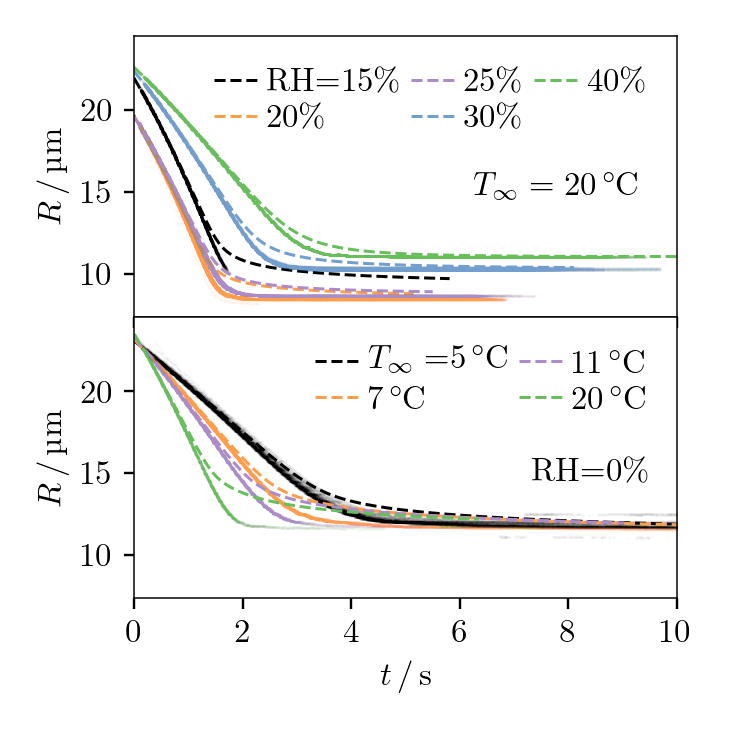
\includegraphics[width=0.9\linewidth,outer]{nano3-trajectory}
  \caption[Evolution of drying droplet radii]{
    Evolution of \ce{NaNO3} aerosol droplet radii from the numerical model (dashed lines) and experiments shown by points with 1\% transparency, showing reasonable agreement at short times until longer times when the evaporation rate is underestimated.
    a) varying relative humidity while ambient temperature is kept fixed, for an initial solute mass fraction of $Y^{(s)} = 0.125$.
    b) varying ambient temperature while relative humidity is kept fixed, for an initial solute mass fraction of $Y^{(s)} = 0.2$.}
  \label{fig:nano3-trajectory}
\end{SCfigure}

We discretise the solute concentration profile $\rho^{(s)}(r)$ onto a uniformly spaced grid over $r \in [0, R(t)]$.
To handle the moving boundary it is convenient to work in the rescaled coordinate $\tilde{r} = \frac{r}{R(t)} \in [0, 1]$.
For the discretisation we define the vector $\vec{\rho} := \{\rho_0, \rho_1, \cdots, \rho_N\}$ where $\rho_i := \rho^{(s)}\left(\tilde{r} = \frac{i}{N}\right)$.
The complete history of the evolution of the droplet then involves both $\vec{\rho}$ and $R$ variables.
In addition, it is convenient to introduce $\dot{R}$ as its own variable so that the final Jacobian for the diffusion equation \eqref{eq:final-diffusion} has tridiagonal form.
This gives us the evolving droplet state variable $\vec{x} = (\vec{\rho}, R, \dot{R})$.

To integrate a timestep $\Delta t$ we use the Crank-Nicolson \cite{CrankMPCPS1947} method where
\begin{equation*}
  \frac{\vec{x}(t + \Delta t) - \vec{x}(t)}{\Delta t}
  =
  \frac{1}{2}
  \left(
  \left. \frac{\partial \vec{x}}{\partial t} \right|_{t + \Delta t}
  +
  \left. \frac{\partial \vec{x}}{\partial t} \right|_t
  \right)
  + \mathcal{O}(\Delta t^2).
\end{equation*}
As the evolution equations are nonlinear this must be solved iteratively to find a self-consistent solution.
Introducing the $k$th approximation for $\vec{x}(t + \Delta t)$ as $\vec{x}^{(k)}(t + \Delta t)$, we write the next term in the sequence as $\vec{x}^{(k+1)} = \vec{x}^{(k)} + \delta \vec{x}^{(k)}$
We obtain
\begin{equation*}
  \frac{\vec{x}_{n+1}^{(k)} + \delta\vec{x}_{n+1}^{(k)} - \vec{x}_n}{\Delta t}
  =
  \frac{1}{2}
  \left(
  \frac{\partial (\vec{x}_{n+1}^{(k)} + \delta\vec{x}_{n+1}^{(k)})}{\partial t}
  +
  \frac{\partial \vec{x}_n}{\partial t}
  \right)
\end{equation*}
using the subscript $n$ as shorthand for the time.
This is a matrix equation that can be inverted for $\delta \vec{x}^{(k)}$.
Convergence is deemed to occur where $\delta \vec{x}^{(k)}$ falls below some threshold value.
The main advantage of this scheme over more simple schemes (e.g. forward Euler method where just the initial $\frac{\partial \vec{x}_n}{\partial t}$ is taken) is that the error is of order $\Delta t^2$ ensuring rapid convergence with small timesteps.

We integrated initially homogeneous droplets of \ce{NaCl} and \ce{NaNO3} for various ambient conditions.
The resulting radius , illustrated for \ce{NaNO3} in Fig.\ \ref{fig:nano3-trajectory}; we see that at short times there is excellent agreement, but the evaporation rate is underestimated at longer times.
This is likely do to limitations of the simplified evaporation model \eqref{eq:sherwood-correction} or because the neglect of conductive forces causes the evaporation to become diffusion-limited at long-times when the surface is highly enriched.
We achieve good agreement with experiments for \ce{NaCl} across their entire time-evolution (Fig.\ \ref{fig:nacl-trajectory}(b)) because these droplets crystallise before the slowdown of the evaporation rate.

\section{Nucleation model}
\label{sec:nucleation}

\subsection{Droplet nucleation rates}

\begin{SCfigure}
  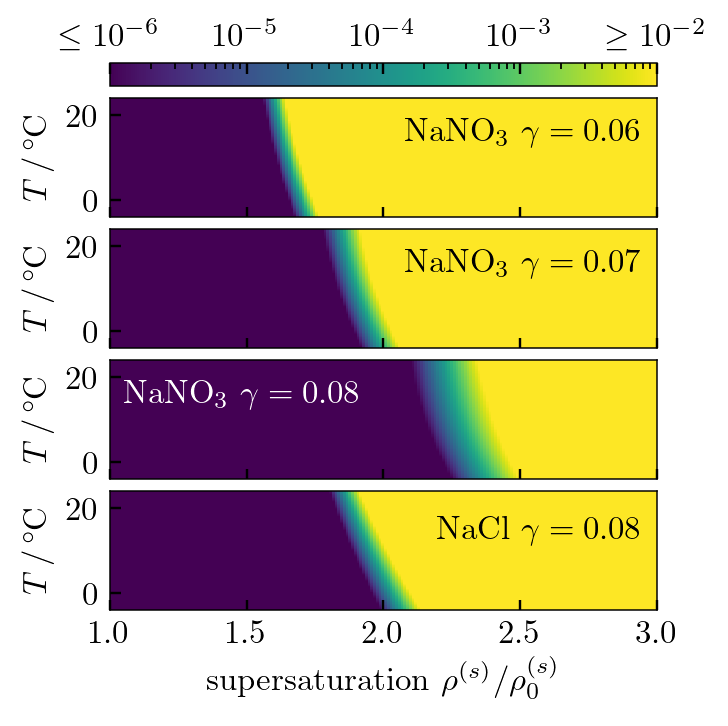
\includegraphics[width=0.9\linewidth,outer]{aerosol-cnt}
  \caption[Nucleation rates predicted by classical nucleation theory]{
    Shell nucleation rate $J\xi$ (\si{\per\micro\metre\squared\per\second}) predicted by classical nucleation theory for aqueous \ce{NaNO3} and \ce{NaCl} solutions at different state points.
    The dark blue and bright yellow regions show where nucleation is essentially impossible or instantaneous on the experimental timescale.
    Different estimates of solid-liquid surface tension $\gamma$ (given in \si{\newton\per\metre}) do not result in a different qualitative picture: a nucleation rate which monotonically increases with supersaturation and temperature.}
  \label{fig:cnt}
\end{SCfigure}

Denoting the rate of solute nucleation per unit volume as $J$, the continuum limit nucleation rate for the entire droplet is
\begin{equation}\label{eq:droplet-nucleation-rate}
  W
  =
  \int_V J dV
  =
  4\pi \int_0^R J(r) \, r^2 dr.
\end{equation}
Both the local $J$ and total rates $W$ contain an implciit time dependence because of their dependency on the evolving variables $R$, $\rho^{(s)}$ and $T$.
For homogeneous nucleation $J$ depends solely on the state variables $\rho^{(s)}$ and $T$.
Nucleation rates are typically strongly concentration dependent \cite{ValerianiJCP2005,DesarnaudJPCL2014,SearJPCM2007}, so we anticipate nucleation to occur at the boundary $r=R(t)$ where the solute concentration is greatest.
Allowing for heterogeneous nucleation $J$ could acquire an additional dependence on the inhomogeneities in the system; as the experiments were performed with high-purity precursor compounds to mitigate the effect of chemical impurities, we expect the main potential site for heterogeneous nucleation to be the liquid-air interface.
Whichever nucleation mechanism dominates, we expect it to occur at the boundary so the total rate \eqref{eq:boundary-nucleation-rate} reduces to
\begin{equation}\label{eq:boundary-nucleation-rate}
  W
  \sim
  4\pi R^2 J \xi
\end{equation}
where $J$ is now evaluated at the boundary, and we introduced $\xi$ as the thickness of the typical shell region over which nucleation occurs.
We will give nucleation rates in terms of $J \xi$, assuming a value $\xi = \SI{1}{\micro\metre}$ to set the absolute scale of the rates predicted by theory (section \ref{sec:cnt}) to most closely match the experiments.

We can relate the nucleation rates to the experimentally observed events by assuming Poisson statistics.
We define the survival probability as
\begin{equation*}
  p_\mathrm{liq}(t)
  :=
  \textrm{Prob}\left[ \textrm{no nucleation by time } t \right],
\end{equation*}
The mean number of nucleation events in the time interval $\Delta t$ is simply $W \Delta t$, giving the probability that there is no nucleation event after a time $\Delta t$ as
\begin{equation*}
  p_\mathrm{liq}(t + \Delta t) = p_\mathrm{liq}(t) e^{-W \Delta t}.
\end{equation*}
Taking the infinitesimal limit and using the fact that droplets are prepared in the liquid state giving the initial condition $p_\mathrm{liq}(t=0) = 1$ yields
\begin{equation}\label{eq:survival}
  p_\mathrm{liq}(t)
  =
  \exp{\left( -\int_0^t W \, dt \right)}.
\end{equation}
As we have already determined the droplet's radius and concentration profile from the evolution equations described in section\ \ref{sec:evolution}, we are left needing a model for the nucleation rate per unit volume $J$ before we can determine $p_\mathrm{liq}$.

\subsection{Nucleation models}
\label{sec:cnt}

%From \eqref{eq:cnt-barrier} we expect a homogeneous nucleation rate per unit volume as
For nucleation processes with a single barrier the rate per unit volume goes as
\begin{equation}\label{eq:nucleation-rate-barrier}
  J = \kappa \exp{\left(-\frac{\Delta G^{*}}{k_B T}\right)}
\end{equation}
where $\kappa$ is a kinetic prefactor and $\Delta G^*$ is thermodynamic barrier for the process.
A widely used approximation for the kinetic prefactor is \cite{SearJPCM2007}:
\begin{equation}
  \kappa = n_I j Z
\end{equation}
$n_I$ is the number density of potential nucleation sites, $j$ is the rate of aggregation to these sites, and $Z$ is the Zeldovich factor.
These last two quantities are typically further approximated as \cite{SearJPCM2007}
\begin{subequations}
  \begin{align}
    j &\sim n D_\mathrm{eff} R^* \\
    Z &\sim (N^*)^{-\tfrac{2}{3}}
  \end{align}
\end{subequations}
where $n$ is the solute number density, $N^*$ is excess number of molecules in the critical nucleus and $R^*$ is its radius.
The barrier $\Delta G^*$ depends on the specific nucleation mechanism.

For homogeneous nucleation the sites of nucleation are simply the solute molecules themselves so $n_I = n$.
The driving force for the transition is the chemical potential change $\Delta \mu$ from formation of the new phase.
In classical nucleation theory (CNT) the surface tension between the crystal and liquid is imagined as the main obstacle to nucleation.
Combining the two contributions leads to the barrier
\begin{equation}
  \Delta G = \gamma A - |\Delta \mu| n_c V
\end{equation}
where $n_c$ is the crystal number density, and $A, V$ are the surface areas and volumes of the nucleated region.
The thermodynamic barrier to nucleation is then the maximum of this formula; assuming a perfectly spherical crystal seed this gives
\begin{align}\label{eq:cnt-barrier}
  \Delta G^{*} &= \frac{4}{3} \pi (R^{*})^2 \gamma \\
  (R^{*}) &= \frac{2\gamma}{n_c |\Delta\mu|}.
\end{align}
The chemical potential expressed in terms of mean ionic activity is\cite{DesarnaudJPCL2014}
\begin{equation}
  %\exp{\left(
  \frac{\Delta \mu}{k_B T}
  %\right)}
  =
  2 \ln{\left( \frac{a_\pm}{a_{0\pm}} \frac{\rho^{(s)}}{\rho^{(s)}_0} \right)}
\end{equation}
where $a_\pm$ is mean ionic activity coefficient, $a_0$ is its value at saturation and $\rho^{(s)}_0$ is the threshold saturation concentration.

We find that CNT predicts homogeneous nucleation rates which increase monotonically in both concentration and temperature.
In Fig.\ \ref{fig:cnt} we show the predicted rates for \ce{NaCl} with $\gamma=\SI{0.08}{\newton\per\metre}$ and \ce{NaNO3} with different estimates of surface tension; we find that the rates increase so rapidly with concentration that they are essentially a step function over the timescale of the experiments.
This is qualitatively correct for \ce{NaCl}, so we are able to accurately predict the time of nucleation in the experiments shown in Fig.\ \ref{fig:nacl-trajectory}.
By contrast, the experiments show that the final survival probability for \ce{NaNO3} droplets is often in the range $0 < p_\mathrm{liq} < 1$ which is not consistent with nucleation rates being characterised by a step function, which we will make more quantitative in the next section.

\begin{SCfigure}
  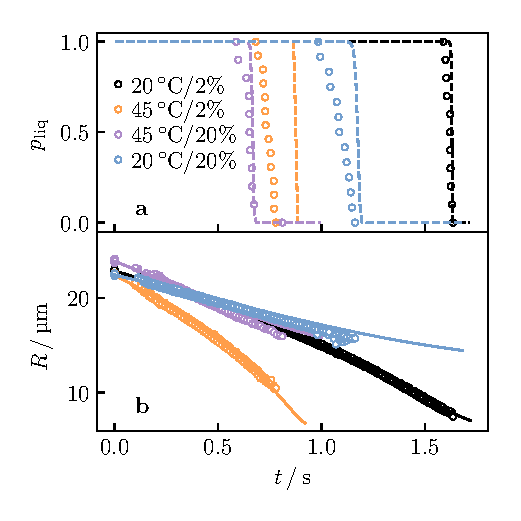
\includegraphics[width=0.9\linewidth,outer]{nacl-trajectory}
  \caption[Evolution of \ce{NaCl} droplets: theory and experiments]{
    Evolution of \ce{NaCl} droplets in dry air $\mathrm{RH}=0\%$ from experiments (points) and the numerical model (lines) for different ambient temperatures and initial solute mass fractions.
    a) the probability that a droplet survives without nucleating, assuming the liquid-crystal surface tension $\gamma = \SI{0.08}{\newton\per\metre}$ \cite{DesarnaudJPCL2014} for the numerical model.
    b) the evolution of droplet radius showing good treatment of solvent evaporation rates.
  }
  \label{fig:nacl-trajectory}
\end{SCfigure}

\subsection{Inferring nucleation rates from experiments}

We can try to determine the nucleation rates directly from experiments by observing the stochastic nucleation behaviour over repeat trajectories and comparing these against the numerical model.
The experiments give us the true survival probabilities $p_\mathrm{liq}$ of which we can determine the droplet nucleation rate $W$ exactly by numerical differentiation.
Combined with the numerical model, which gives us the precise state of the droplet, we can infer $J\xi$ from inversion of the rate formula \eqref{eq:boundary-nucleation-rate} under the assumption that nucleation is boundary-dominated.
%% We can make some progress by making some strong assumptions about the form of $J \xi$ based on physical intuition.
%% We will then test for self-consistency to justify this approach in an ad-hoc manner.

Differentiation of the survival probability \eqref{eq:survival} yields
\begin{equation}
  \dot{p}_\mathrm{liq}
  =
  - W p_\mathrm{liq},
\end{equation}
upon combining this with our assumption that nucleation occurs near the boundary \eqref{eq:boundary-nucleation-rate} allows to write the nucleation rate as
\begin{equation}
  J\xi
  =
  - \frac{1}{4\pi R^2} \frac{\dot{p}_\mathrm{liq}}{p_\mathrm{liq}}
\end{equation}
which we can determine from the experimentally observed $p_\mathrm{liq}$ trajectory.
The derivative of $p_\mathrm{liq}$ can be obtained through fitting.
The survival probabilities decay monotonically as a generalised step function, so we fit the experimental trajectories with the Fermi-Dirac form
\begin{equation}
  p_\mathrm{liq}(t) - \lim_{t \to \infty} p_\mathrm{liq}(t)
  =
  \frac{1 - \lim_{t \to \infty} p_\mathrm{liq}(t)}{\exp{\left[\epsilon(t - t_s)\right]} + 1}
\end{equation}
where $t_s$ is the time at which saturation is reached $\rho^{(s)}(R) = \rho^{(s)}_0$, and introducing the fitting function
\begin{equation*}
  \epsilon(t)
  =
  \begin{cases}
    at + bt^2 - c / t & \; t > 0 \\
    - \infty & \; t < 0
  \end{cases}
\end{equation*}
subject to the constraint that the fitting parameters $a, b, c \in [0, \infty]$ to ensure that $p_\mathrm{liq}$ decreases monotonically from $p_\mathrm{liq}(t=0)=1$.

We perform this inversion procedure for the \ce{NaNO3} droplets in Fig.\ \ref{fig:state-points}(b).
The resulting nucleation rates show non-mononic behaviour, increasing to a maximum before decreasing to essentially zero over the duration of the experiment.
This results in a finite final survival probability $p_\mathrm{liq} > 0$, and starkly contrasts with the picture predicted by CNT where $p_\mathrm{liq}$ would remain close to unity for most of the experiment before sharply dropping to zero as all droplets reproducibly crystallise.

\begin{SCfigure}
  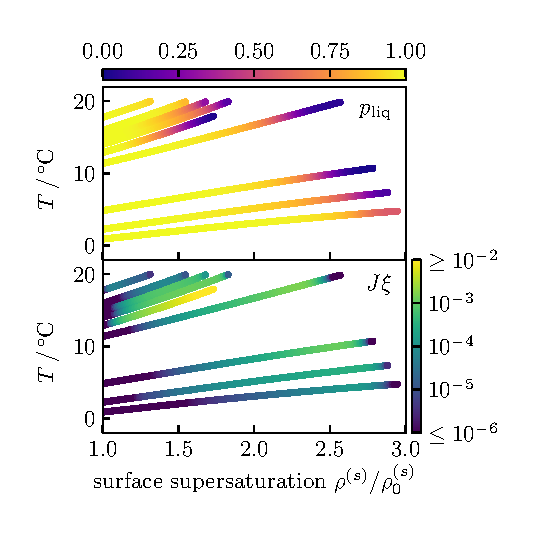
\includegraphics[width=0.9\linewidth,outer]{nano3-nucleation-rates}
  \caption[Experimentally observed nucleation rates in \ce{NaNO3} droplets]{
    State points explored by experiments with drying \ce{NaNO3}--\ce{H2O} aerosol droplets as determined from our numerical model for 9 datasets for different initial conditions.
    a) the survival probability in the experiments (i.e.\ the probability that a droplet has not crystallised), with state-point inferred from the model.
    b) the corresponding nucleation rates assuming boundary-dominated nucleation \eqref{eq:boundary-nucleation-rate} showing non-monotonic behaviour in increased concentration and temperature in contrast with the predictions of classical nucleation theory in Fig.\ \ref{fig:cnt}.}
  \label{fig:state-points}
\end{SCfigure}

\section{Conclusions}

We have developed a numerical model based on a diffusion equation with an extrapolation of the diffusion constant to high concentrations assuming the Stokes-Einstein relation.
The resulting droplet evolution conforms well to the experimental trajectories.
Assuming boundary dominated nucleation we are able to predict nucleation rates inside the droplet, and extract nucleation rates at differing state points from the experimental trajectories.

We found that CNT works well for predicting crystal nucleation in \ce{NaCl} but not \ce{NaNO3} aerosols.
In both cases CNT predicts nucleation essentially after a threshold surface saturation is reached, whereas experiments show nucleation in \ce{NaNO3} has stochastic behaviour.
This emerges from the fact that nucleation rates predicted by CNT monotonically increase in concentration and temperature.
In particular, the change in nucleation rate from increased concentration is so dramatic that the behaviour of CNT is essentially unchanged by small adjustments to the model parameters.

CNT is a model for homogeneous nucleation, so it is possible that it fails because crystallisation occurs for \ce{NaNO3} through heterogeneous nucleation.
The same stochastic phenomena are observed when repeating the experiments with the same droplet on a cycle of decreasing and increasing the RH to dry and melt the droplet; this rules out heterogeneous nucleation through impurities, as the chemical makeup is the same in each cycle yet the phenomenon persists.
This leaves the gas-liquid phase boundary itself as a site for hetereogeneous nucleation.

It is highly likely that the model overestimates the surface enrichment because at long times the simulated evaporation rates become limited by solute diffusion at the boundary.
The diffusion limit would persist even if more sophisticated transport phenomena were introduced to the evaporation model.
Surface enrichment is overestimated because we have neglected the effect of temperature gradients inside the droplet, and because we have used an extrapolation of low concentration diffusion data which likely to underestimate diffusion at high concentrations.
Temperature gradients create inward convection currents reducing surface enrichment.
Our extrapolation of the diffusion constant assumed the Stokes-Einstein relation holds across the whole state space, however this relation can be violated at high viscosities \cite{BerthierRMP2011}.
The rapid increase of viscosity with salt concentration in our model leads to a feedback loop where diffusion becomes increasingly difficult as the surface is enriched.
Correcting for these effects, we expect the surface concentrations explored by the experiments to increase to a maximum before decreasing which could explain non-monoticity.
However, this can only partially explain the observed behaviour because CNT is extremely sensitive to concentration.

%Our evaporation model considerably simplifies the transport phenomena at the phase boundary, though it becomes limited by the rate of solute diffusion at the boundary at long times suggesting that we are underestimating the rate of mixing.

%It is possible that our assumption that kinetics occurs purely through Fickian diffusion oversaturates the solute at the boundary, complicating our analysis of the nucleation rate.
%To go beyond this one would have to model temperature gradients to allow for conduction forces which help keep the droplet well-mixed.

This work is important in showing that the nucleation rate of nitrate aerosol is not only influenced by the level of supersaturation, but also by the drying kinetics itself because of an interplay between the inhomogeneity of the concentration profile and droplet temperature.
This is important for climate predictions where an understanding of the phase of atmospheric aerosol is crucial, and also valuable for spray-drying models where control over the resulting phase could be enabled by tuning the various drying parameters.

%% It is unlikely to be due to the trajectories being incorrect: even varying the most poorly estimated parameter for \ce{NaNO3}, the surface tension, does not change the CNT prediction.
%% Because of the sensitivity of CNT on parameters, it would require a remarkable degree of fine tuning to fit CNT model with any physically plausible parameters.
%% It's possible nucleation of \ce{NaNO3} occurs via a more complex kinetic pathway, e.g.\ multiple steps \cite{?,?,?}.
%% Alternatively, the experimental nucleation could be occurring via heterogeneous nucleation (e.g.\ impurities in the sample).
%% This is unlikely however, as the experiments can maintain the same salt sample and follow the single trajectory and it will still show the same stochastic behaviour.
%% Impurities are not likely to be in the solvent, or we would likely see the same phenomenon in \ce{NaNO3} nucleation.

%An option would be to relax the assumption that the temperature of the droplet is constant, as convection effects could play a key role in mixing the solution.
%Solving the Navier-Stokes equations would be essentially exact, though expensive route to include this.
%Less expensive would be to use vortex models or effective-conduction models which treat the internal circulation/convection of heat in an ad hoc manner.

\ifdefined\includebibliography
  \printbibliography
\fi

\end{document}

%TC: macro \marginfootnote [other]
%TC: envir SCfigure [] other
%TC: macrocount beginSCfigure [figure]
\documentclass[11pt,twoside]{report}
\usepackage{preamble}
\setcounter{chapter}{7}
\graphicspath{{../img/}}
\def\includebibliography{}

\externaldocument{background}
\externaldocument{supercooled-liquids}
\externaldocument{morphometric-framework}
\externaldocument{morphometric-applications}
\externaldocument{resummation}
\externaldocument{aerosols}

\begin{document}
\chapter{Conclusion}
\epigraph{We demand rigidly defined areas of doubt and uncertainty!}{Douglas Adams, \emph{The Hitchhiker's Guide to the Galaxy}, (1979).}

At high densities, the dynamical properties of supercooled liquids show marked complexity distinguishing them from their ordinary counterparts at lower densities.
We have attempted to develop methods to better understand the nature of dynamical arrest and the glass transition, and nucleation of crystals within the metastable liquid.
Most of this work has focused on the first question, so we will emphasise that topic here and return to nucleation towards the end.

%with hard spheres as the model system, and to address nucleation of the crystals in a real system.
%Specifically, supercooled liquids and the glass transition, and nucleation of the crystal.

Liquids approaching their glass transition display a dramatic slowdown in their relaxation behaviour, while showing no obvious structural change at the level of pair correlations.
In chapter \ref{chapter:glass} we summarised the various scenarios posited to explain this phenomenon, highlighting the potential role of amorphous order in mean-field theories and structural order in geometric theories.
These thermodynamic scenarios in particular posit solely static mechanisms for dynamic arrest, which we argued could be detected through the many-body correlation functions.
Developing from this observation, in chapter \ref{chapter:morphometric-framework} we showed that the correlation functions could be expressed in terms of a potential of mean force, itself dependent on the interaction potential and a chemical potential term.
The key approximation we employed was the \emph{morphometric approach}, where the chemical potential is expressed as an expansion in size measures: the volume, surface area and integrated curvature measures.
Using the many-body correlation functions we attempted to explore the energy landscape of local structures in chapter \ref{chapter:morphometric-applications}, to look for features which could be connected with dynamical arrest.

%Disappointingly we have few results.

We have presented three justifications of the morphometric approach for hard particle systems.
First, we derived it in the usual way as a limit of fundamental measure theory (section \ref{sec:fmt}).
Second, we argued for the morphometric \emph{ansatz} as the natural generalisation of scaled particle theory (chapter \ref{chapter:morphometric-framework}); furthermore, we used integral geometry to argue that this \emph{ansatz} generalises the form of an extensive quantity (section \ref{sec:generalised-intrinsic-volumes-d}).
And last, we derived the morphometric form for the chemical potential by resumming a component of the virial series (chapter \ref{chapter:resummation}).

The latter two justifications are in principle new arguments, though we suspect neither will be of any surprise to the liquid state community; in some sense, these routes are all equivalent because they fundamentally reduce to integral geometric arguments.
%, and properties of the intrinsic volumes.
The primary advancements of this work have thus been technological, rather than fundamental, in nature.
In particular, we introduced the trick of imposing self-consistency of the virial theorem to derive a new set of morphometric coefficients in hard spheres (chapter \ref{chapter:morphometric-framework}).
These coefficients yield a theory for chemical potentials capable of producing highly accurate correlation functions, even at high densities.
Although we have made some modest contributions to treating local structure in chapter \ref{chapter:morphometric-applications} (described below), fundamentally the accuracy of all subsequent results depended on application of this trick.

In chapter \ref{chapter:morphometric-applications} we introduced methods to extend the formalism of energy landscapes, normally applied to soft potentials, to local structures of hard spheres; many adaptations were required to handle the singularity of the hard sphere interaction potential.
%Concerning morphometric approach: most of the developments have been in methods.
We explored a method of predicting the concentrations of structural motifs within the liquid, and developed a route to do similar calculations along saddles
%\marginfootnote{These calculations used techniques from Bayesian inference which were a late addition to this thesis, and are subsequently the least well-explained.
%  Their inclusion provides a route to extending calculations to dynamical phenomena, so I felt it important to include them for a more complete perspective of available options.}
for connecting with dynamics.
Notably, we found a bimodality in the distribution of energy states corresponding to distinct structural symmetries, of potential importance to structural viewpoints of dynamical arrest.
This work lays the groundwork for a quantitative assessment of the landscape properties of local regions within the liquid, which could explore the validity of random first-order transition and related theories.

There are two limits to the accuracy of the morphometric approach: the thermodynamic coefficients entering the theory, and the limitations \emph{ansatz} itself.
We found that improving the coefficients was enough to obtain accurate results in chapters \ref{chapter:morphometric-framework} and \ref{chapter:morphometric-applications}, though the theory was not exact and so there is room for improvement particularly at high densities.
We attempted to provide some insight into the theory behind the morphometric approach in chapter \ref{chapter:resummation}, with a view to potentially supplementing the \emph{ansatz} with additional terms.
There, we found a contribution to the chemical potential which is rigorously of morphometric form, the thermodynamic coefficients of which capture most of the bulk free energy in hard spheres up to moderate densities; this observation potentially explains why the approach works well in the first place.
Furthermore, the resulting theory applies to arbitrary mixtures of hard convex particles without modification of the morphometric \emph{ansatz}, suggesting that extensions to other hard particle systems are possible.

%% Generalisations:
%% Hard particle extension is done.
%% We tested the theory up to mode-coupling, finding it accurate.
%% Polydisperse ready to go: direct comparison with the high density swap data could be made.
%% Could be a challenge to do the virial route coefficients, 
%% By introducing polydispersity into the theory we should obtain better quantitative agreement with experiments and simulations.

In Refs.\ \cite{DamascenoS2012,DamascenoAN2012} Glotzer and coworkers showed that hard polyhedra have all the richness in phase behaviour of the periodic table.
For example, the propensity for glassformation can be increased by inducing competition between polyhedra of different symmetries, which form competing domains of incompatible crystal structures \cite{TeichNC2019}.
Subsequent developments have introduced methods for tailoring the assembly into target crystal structures \cite{YoungACIE2013,SchultzAN2015,VanAndersAN2015}, many of which have been observed in simulation and experiment \cite{MisztaNM2011,HenzieNM2012,QiJCP2013}.
Polyhedral particles are intended as representatives of anisotropic particles (e.g.\ nanoparticles and colloids), in the same way that hard spheres are the starting point in simple liquids.
In current theories \cite{YoungACIE2013} effective entropic forces are imagined between parallel faces of adjacent polyhedra, which becomes exact at asymptotically high pressures.
The morphometric approach thus has potential to significantly improve descriptions of these interactions, and become a quantitatively predictive theory for nanoparticle and colloidal self-assembly.
%This would probably be the most interesting extension of the morphometric calculations.

For the \emph{isotropic} phase the current morphometric approach should readily extend to arbitrary mixtures of convex polyhedra; the form of the Carnahan-Starling equation for mixtures \eqref{eq:cs-mixtures} should even give a reasonable description of the liquid pressure.
However, in practice the computational geometry required to actually extend morphometric calculations to non-spherical particles would present a considerable challenge.
For \emph{anisotropic} phases (e.g.\ liquid crystal phases which form for highly elongated polyhedra) further theoretical developments would be required.
Fundamental measure theory has been extended to anisotropic phases \cite{Hansen-GoosPRL2009,Hansen-GoosJPCM2010,WittmannEL2015,WittmannPRE2015,WittmannJPCM2016}, so it is likely that a similar programme could be achieved for the simpler morphometric approach.

Continuing on the theme of self-assembly, a fundamental development of interest would be to the kinetics of protein folding.
The entropy of the surrounding water is argued to be a major thermodynamic contribution for aqueous proteins \cite{HaranoCPL2004,HaranoBJ2005,KinoshitaCES2006}.
The morphometric approach would thus be desirable to avoid explicit solvent modelling, and it has been used with some success \cite{HaranoCPL2006,RothPRL2006,KodamaJCP2011}.
Most of the literature on the morphometric approach concerns hard particles so, while it seems to accurately treat depletion/exclusion interactions, it is less clear how well it would perform for softer interaction potentials with attractions which better represent real systems.
Notably, the presence of attractions can induce non-analytic contributions through surface phase transitions \cite{EvansELE2003,EvansJCP2004}, which cannot be captured by the morphometric \emph{ansatz}.
Moreover, with a soft potential it is not clear \emph{a priori} how to define the surface geometry.
Despite these concerns, the potential computational benefit of the morphometric approach makes this area worth exploring.

Finally, we studied the nucleation of salt crystals inside atmospheric aerosols in chapter \ref{chapter:aerosols}.
The chemistry involved was too complex to treat the nucleation kinetics with a hard sphere model, so we used a continuum diffusion model to understand experimental data.
We found that classical nucleation theory had mixed success for the systems studied, suggesting more complex nucleation pathways than a simple one-dimensional model.

Were the morphometric approach to be extended to more realistic potentials, we could imagine bridging the gap between the microscopic models of the hard sphere chapters and the continuum models of the final chapter.
Crystal nucleation occurs by spontaneous formation of a crystal domain inside the bulk liquid, so the free energy calculations of chapter \ref{chapter:morphometric-applications} could be used for crystal geometries to assess the thermodynamic driving forces of nucleation.
The morphometric approach would offer a route to access nucleation pathways of much greater complexity than the simple one-dimensional projection normally considered in classical nucleation theory.
This would be another logical avenue of the morphometric approach, of interest even for hard spheres.

\ifdefined\includebibliography
  \newgeometry{margin=1in}
  \printbibliography
\fi

\end{document}


\begin{appendices}
  %TC: macro \marginfootnote [other]
%TC: envir SCfigure [] other
%TC: macrocount beginSCfigure [figure]
\documentclass[11pt,twoside]{report}
\usepackage{preamble}
\setcounter{chapter}{0}
\graphicspath{{../img/}}
\def\includebibliography{}
\renewcommand{\chaptername}{Appendix}
\renewcommand{\thechapter}{\Alph{chapter}}

\begin{document}
\chapter{Singularities in the hard sphere chemical potential}
\label{appendix:spt-singularities}

Here we show that the cost of inserting a solute is not generally analytic in geometric measures by revisiting the arguments made by Reiss and coworkers \cite{ReissJCP1959,ReissJCP1960}.
This argument is worth revisiting as it demonstrates that \emph{any} regular expansion of $\Delta \Omega$ in terms of geometrical measures like curvature must necessarily be approximate.
In sections \ref{sec:morphometric-theory} and \ref{sec:spt} we will contribute to the theory of such an expansion, so the purpose of this section is to emphasise its approximate nature from the outset as a disclaimer.
\todo{Fix references and make this appendix more thesis-y}

We consider a single-component hard sphere liquid with particles of diameter $\sigma$, and we imagine inserting a hard spherical solute of radius $R$.
A sphere of radius $R + \sigma/2$ around the solute is excluded to the centers of solvent particles.
We write this excluded volume as $V_\mathrm{ex}$, which is clearly the minimum size of cavity required to contain the solute.
The insertion cost is simply the probability that a randomly chosen position for insertion contains such a cavity, i.e.\
\begin{equation}\label{eq:insertion-from-p}
  \Delta \Omega(R)
  =
  -k_B T \ln p_0(R)
\end{equation}
where $p_0$ is the probability that the excluded region is empty.
This can be determined as \cite{ReissJCP1959}
\begin{equation}\label{eq:spt-zero-cavity-p}
  p_0(R) = 1 + \sum_{n=1}^\infty (-1)^n F^{(n)}(R)
\end{equation}
where $F^{(n)}(R)$ is the average number of $n$-tuples of solvent particles contained in the excluded region, as in
\begin{equation}\label{eq:spt-tuple-function}
  F^{(n)}(R)
  =
  \frac{\rho^n}{n!}
  \int_{V_\mathrm{ex}^n} g^{(n)}(\vec{r}^n) \, d\vec{r}^n.
\end{equation}
Clearly $F^{(n)}(R) = 0$ for $R < R_n$, the minimum radius capable of containing $n$ hard spheres.
At any given state point $g^{(n)}$ will be bounded from above by some finite number, so we can write the inequality
%\footnote{Typically we would expect this to occur where the maximum number of particles are in contact, however that is not a necessary assumption for this argument.},
\begin{equation}\label{eq:spt-tuple-function-upper-bound}
  \begin{split}
    F^{(n)}(R) &\le
    \frac{\rho^n}{n!}
    \max_{\mathbb{R}^{dn}}{\left(g^{(n)}\right)}
    \int_{V_\mathrm{ex}} \, d\vec{r}^n \\
    &=
    \frac{\rho^n}{n!}
    \max_{\mathbb{R}^{dn}}{\left(g^{(n)}\right)}
    (V_\mathrm{ex})^n,
  \end{split}
\end{equation}
but because of the hard core interaction there will be heavy restrictions on allowable values of $n$ for any $R$.
Defining $R_n$ as the smallest $R$ such that $n$ particles can be accommodated, we expect
\begin{equation}\label{eq:F-scaling}
  F^{(n)}(R) =
  \begin{cases}
    0 & \quad R < R_n \\
    \mathcal{O}\left( \left(V_\mathrm{ex}\right)^n \right) & \quad R > R_n
  \end{cases}
\end{equation}
where the latter polynomial is motivated by the same argument as used in \eqref{eq:spt-tuple-function-upper-bound}.
Noting that $V_\mathrm{ex} \propto R^d$ this can be expressed alternatively as a polynomial in $R$.
\begin{equation*}
  F^{(n)}(R) =
  \begin{cases}
    0 & \quad R < R_n \\
    \mathcal{O}\left( R^{dn} \right) & \quad R > R_n
  \end{cases}
\end{equation*}
Applying this bound to \eqref{eq:spt-zero-cavity-p} gives bounds on the scaling of $p_0$ as
\begin{equation}\label{eq:spt-p-scaling}
  p_0(R) =
  \mathcal{O}\left( R^{dn} \right)
  \quad R_n < R < R_{n+1}.
\end{equation}
From \eqref{eq:spt-p-scaling} we expect to see singular behaviour at the points $\{R_n\}$.
To look at this in more detail we define
\begin{equation*}
  p_0^{(n)}(R) := 1 + \sum_{m=1}^n (-1)^m F^{(m)}(R)
\end{equation*}
such that $p_0 = p_0^{(n)}$ for $R \le R_{n+1}$.
Approaching the singular point $R_n$ we find the deviation from the solution for $R < R_n$ is thus
\begin{equation*}
  \begin{split}
    \Delta p_0(R) &:=
    p_0(R) - p_0^{(n-1)}(R)
    \\ &=
    (-1)^n F^{(n)}(R)
    \qquad R < R_{n+1}
  \end{split}
\end{equation*}
i.e.\ the singular behaviour is entirely contained in $F^{(n)}$.
Noting that polynomials of degree $n$ have vanishing $(n+1)$th derivatives, and $V_\mathrm{ex} \propto R^d$, we thus expect a discontinuity in the $dn$th derivative of $p_0$ about $R=R_n$; from \eqref{eq:insertion-from-p} we find $\Delta \Omega$ will similarly feature a discontinuity in its $dn$th derivative at $R=R_n$.
A summary of the first few singularities in three-dimensions is given in Table~\ref{table:spt-singularities}.

Again, these singularities have long been known since the first papers on scaled particle theory \cite{ReissJCP1959,ReissJCP1960}.
They are worth reiterating because any geometric expansion in simple powers of $R$ will not capture these singularities; the morphometric approach is an example of such an expansion, albeit generalised beyond spherical solutes, so it must necessarily be approximate.

\begin{SCtable}
  \begin{minipage}[b]{\linewidth}
    \centering
    \begin{tabular}{ccc}
      \toprule
      $n$ & $R_n / \sigma$ & Discontinuity \\
      \midrule
      %% 2 & $\frac{\sigma}{2}$ & $\Delta \Omega'''(R)$
      %% \\
      %% 3 & $\frac{\sigma}{\sqrt{3}}$ &
      %% $\dfrac{\partial^6 \Delta \Omega}{\partial R^6}$
      %% \vspace{0.25em} \\
      %% 4 & ${\sqrt{\frac{3}{8}}} \sigma$ &
      %% $\dfrac{\partial^9 \Delta \Omega}{\partial R^9}$
      2 & 0 & $\Delta \Omega'''(R)$
      \\
      3 & $\dfrac{1}{\sqrt{3}} - \dfrac{1}{2}$ &
      $\dfrac{\partial^6 \Delta \Omega}{\partial R^6}$
      \vspace{0.25em} \\
      4 & $\sqrt{\dfrac{3}{8}} - \dfrac{1}{2}$ &
      $\dfrac{\partial^9 \Delta \Omega}{\partial R^9}$ \\
      \bottomrule
    \end{tabular}
  \end{minipage}
  \caption[First few singularities in the insertion cost]{
    First few singularities in the cost of inserting a sphere of radius $R$ into a one-component hard sphere liquid of diameter $\sigma$ in $d=3$.
    $R = R_n$ is the minimum radius required for a sphere to contain $n$ spheres, and the corresponding singularity is determined from equations \eqref{eq:insertion-from-p} and \eqref{eq:spt-p-scaling}.}
  \label{table:spt-singularities}
\end{SCtable}

\ifdefined\includebibliography
  \printbibliography
\fi

\end{document}

  %TC: macro \marginfootnote [other]
%TC: envir SCfigure [] other
%TC: macrocount beginSCfigure [figure]
\documentclass[11pt,twoside]{report}
\usepackage{preamble}
\setcounter{chapter}{1}
\graphicspath{{../img/}}
\def\includebibliography{}
\renewcommand{\chaptername}{Appendix}
\renewcommand{\thechapter}{\Alph{chapter}}

\begin{document}
\chapter{Explicit morphology for two particles}
\label{appendix:two-spheres}

In the previous section we gave computational details for calculating morphological quantities of the solvent accessible surfaces.
Here we give the explicit form for the special case where there are two particles.
These formulas can provide some intuition for the general case, and will be directly used in section \ref{SI:coefficients} to derive new thermodynamic coefficients.
\todo{Tidy this appendix up so it is more thesis-y, and fix references!}

For two particles $g^{(2)}(\vec{r}_1, \vec{r}_2)$ reduces to $g^{(2)}(|\vec{r}_1 - \vec{r}_2|)$ as the system is completely isotropic.
All morphological quantities are then functions of $r = |\vec{r}_1 - \vec{r}_2|$.
As $r \to 2\sigma$ the solvent accessible surface $\partial\mathcal{L}$ self-intersects, and two separate (perfectly spherical) surfaces form for $r > 2\sigma$.
The Euler characteristic of $\partial\mathcal{L}$ is thus
\begin{equation}
  \chi(r) =
  \begin{cases}
    2 & r < 2\sigma \\
    4 & r > 2\sigma.
  \end{cases}
\end{equation}
Written explicitly, the resulting distribution function is
\begin{equation}\label{eq:g2-explicit}
  g^{(2)}(r) =
  \begin{cases}
    0 & r < \sigma \\
    \exp{\Big(-\beta (pV(r) + \gamma_\infty A(r) + \kappa C(r) + \overline{\kappa} X(r) - 2\mu^{ex})\Big)} &
    \sigma \le r \le 2\sigma \\
    1 & r > 2\sigma.
  \end{cases}
\end{equation}
with morphological quantities
\begin{subequations}\label{eq:g2-explicit-morph}
\begin{align}
  V(r) &= \frac{8\pi}{3} \sigma^3 - (r^2 + 4\sigma r) \frac{\pi (2\sigma - r)^2}{12 r} \, \Theta(2\sigma-r), \\
  A(r) &= 8\pi\sigma^2 - 2\pi\sigma \, (2\sigma-r) \, \Theta(2\sigma-r), \\
  C(r) &=
  8\pi\sigma - 2\pi \, \left[ \sqrt{\sigma^2 - \left(\frac{r}{2}\right)^2} \arcsin{\left(\frac{r}{2\sigma}\right)}
    + (2\sigma-r) \right] \, \Theta(2\sigma-r), \\
  X(r) &= 2\pi \chi(r)
\end{align}
\end{subequations}
where $\Theta(\cdots)$ is the Heaviside step function.
The mean curvature stated is a special case of the more general result worked out in \cite{OettelEL2009}.
The first term of the expressions for $V,A,C$ contains the morphological measures for two \emph{independent} particles (e.g.\ twice the volume of a single particle), whilst the remaining terms are corrections due to their mutual intersections.

\ifdefined\includebibliography
  \printbibliography
\fi

\end{document}

  %TC: macro \marginfootnote [other]
%TC: envir SCfigure [] other
%TC: macrocount beginSCfigure [figure]
\documentclass[11pt,twoside]{report}
\usepackage{preamble}
\setcounter{chapter}{2}
\graphicspath{{../img/}}
\def\includebibliography{}
\renewcommand{\chaptername}{Appendix}
\renewcommand{\thechapter}{\Alph{chapter}}

\begin{document}
\chapter{Computational geometry for the union of many spheres}
\label{appendix:computational-geometry}

\section{Introduction}

The two curvature measures, $C_{\partial\mathcal{L}}$ and $X_{\partial\mathcal{L}}$ (integrated mean and Gaussian curvatures respectively), are required for the morphological thermodynamics used extensively in the main text.
In this section we give details on their geometric construction to aid morphological calculations.
The relevant formulas for $C_{\partial\mathcal{L}}$ and $X_{\partial\mathcal{L}}$ in hard sphere systems have previously been given in references \cite{MeckeAA1994} and \cite{RothPRL2006}.
Here, we restate these formulas and extend them by computing their derivatives with respect to atomic coordinates.
This technical description is only likely to be of interest to those wishing to do morphological calculations of their own.
\todo{Tidy this appendix up so it is more thesis-y, and fix references!}

To briefly motivate these derivative calculations, we remind the reader that derivatives were used in the main text in the calculation of the free energy of local structures along the octahedron-tripyramid reaction path.
Gradients were required for this calculation, providing an analytic method (with perturbation theory) where the numerical method (thermodynamic integration) fails due the instability of intermediate points along the reaction path.
Full details of this method are given in Sec.\ \ref{SI:reaction-path}.
It is worth stating that the usefulness of gradient calculations extends beyond this one application.

The gradient gives the mean depletion forces between (nearby) particles within the bulk liquid, which is generally a quantity of interest in liquid state theories.
These solvation forces are useful for speeding up numerical minimisation procedures, and for describing the solvation forces for molecules and proteins in aqueous solution.
For the latter case one requires a solvent accessible surface $\partial{\mathcal{L}}$ which is composed of balls of varying radii; the formulas we present allow for this generalisation.

\section{Decomposing the solvent accessible surface into intersections}

For correlations in homogeneous liquids composed of identical balls, the curvatures must be computed across the solvent accessible surface $\partial\mathcal{L}$ where the enclosed volume is
\begin{equation*}
  \mathcal{L} = \cup_{i=1}^n B_\sigma(\vec{r}_i).
\end{equation*}
In order to keep the formulas as general as possible, we will consider a small generalisation of this surface where the spheres are of arbitrary radii, i.e.\
\begin{equation}\label{eq:generalised-volume}
  \mathcal{L} = \cup_{i=1}^n B_{\sigma_i}(\vec{r}_i),
\end{equation}
where $\sigma_i$ is the diameter of particle $i$.
One obtains the surface used in the main text by setting $\sigma_i = \sigma$ for all $i$.
Let $K^d \subseteq \mathbb{R}^d$ denote the space of \emph{polyconvex} subsets of $d$-dimensional Euclidean space.
By \emph{polyconvex} we mean subsets composed of a \emph{finite} union of convex subsets; this means the surfaces are well-behaved so standard geometric descriptions and intuitions apply.
By construction $\mathcal{L} \in \mathcal{K}^d$ and $\partial\mathcal{L} \in \mathcal{K}^{d-1}$.

If particle $i$ is on the surface of $\mathcal{L}$, i.e.
\begin{equation*}
  S_i %\equiv \partial B_\sigma(\vec{r}_i)
  \cap \partial\mathcal{L} \notin \emptyset %\in \mathcal{K}^{d-1}
\end{equation*}
where $S_i \equiv \partial B_{\sigma_i}(\vec{r}_i)$ is the spherical surface of particle $i$, then integrals over $\partial\mathcal{L}$ must carefully consider pieces $S_i$ and intersections $\bigcap_i S_i$ separately.
Intersections, e.g.\ $S_i \cap S_j$ for $i \ne j$, contribute zero area, but may have nonvanishing curvature; this is usually understood by considering the parallel surface $\partial(\mathcal{L}+B_\epsilon)$ in the limit as $\epsilon \to 0$.
Hard core interactions ensure pathological cases where spheres share a centre are excluded, so intersections of two spheres must result in a (one) lower dimensional manifold $S_i \cap S_j \in \mathcal{K}^{d-2}$.
It is straightforward to extend this argument to $n \le d$ intersections $\bigcap_{i=1}^{n} S_i \in \mathcal{K}^{d-n}$.
For $n = d$ intersections the solution is a zero-dimensional manifold, i.e.\ a point.

Intersections between $n > d$ spherical surfaces are possible in principle, but in practice they occur with vanishing probability once a system is thermalised.
To see this, consider an overlap of $n > d$ hard spheres.
By the above argument one can decompose the surface of the resulting structure into $k$-dimensional submanifolds where $0 \le k \le d$.
Higher order surface intersections $n>d$ requires multiple $n=d$ intersections to occur at the same point, which is overconstrained and occurs with measure zero.
Thus, the probability of finding points where $n > d$ spheres intersect occurs with measure zero.
This argument only applies because we considered the \emph{boundary} of the intersections; it is more common in the physics literature to consider the Mayer f-function (related to the Euler characteristic) of the intersection \emph{volumes}, where the measure is nonzero leading to slow convergence of the virial series \cite{Hansen2013}.
Despite having zero measure, there are cases where one would construct a geometry containing a higher order intersection so we will return to this topic in more detail in section \ref{sec:higher-order-intersections}.

In summary, for $d=3$ the surface $\partial\mathcal{L}$ contains the following submanifolds:
\begin{itemize}
\item $S_i \cap \partial\mathcal{L} \notin \emptyset$: a spherical cap from particle $i$.
\item $S_i \cap S_j \cap \partial\mathcal{L} \notin \emptyset$ for $i \ne j$: a line, specifically a circular arc.
\item Point $S_i \cap S_j \cap S_k \cap \partial\mathcal{L} \notin \emptyset$ for $i \ne j \ne k$: points where balls $i$, $j$, and $k$ intersect.
  3 intersecting spheres generally have 2 points of intersection, though usually only 1 of these coincides with the surface $\partial\mathcal{L}$ (the other is usually buried inside the volume $\mathcal{L}$).
\item Intersections of more than 3 surface spheres: occurs with vanishing probability in \emph{thermal} systems (see above).
\end{itemize}

In subsequent sections we will detail contributions to $C_{\partial\mathcal{L}}$ and $X_{\partial\mathcal{L}}$ (and their derivatives) from each of these intersections in $d=3$.
Note that for morphological thermodynamics one also requires the volume and surface area contributions, $V_\mathcal{L}$ and $A_{\partial\mathcal{L}}$, for which we do \emph{not} provide computational details as there is already a wealth of literature on this subject (notably Refs.\ \cite{EdelsbrunnerPNAS2003,BryantDCG2004}).
In particular, we found the algorithm in Ref.\ \cite{KleninJCC2011} to be fast and robust.
We extended their implementation to also compute integrated curvature measures, with the formulas given in subsequent sections.

\section{Integrated mean curvature}

\subsection{Notation}

In the main text we expressed the coordinates $\vec{r}^n \in \mathbb{R}^{3n}$ as the direct sum $\vec{r}^n = \vec{r}_1 \oplus \cdots \oplus \vec{r}_n$.
As each line contribution in \eqref{eq:integrated-curvature} depends on the positions of 2 central spheres, whose intersection forms a circle, together with 2 additional spheres whose intersections with the first two spheres creates terminating vertices for the circular arc.
Thus the line contribution depends on the positions of up to 4 particles, so the domain and image of the gradient is (potentially) 12-dimensional.
Fewer particles can be involved, and thus the dimension of the space is reduced, if:
\begin{itemize}
  \item $\theta_{l}^{(1)}$ and $\theta_{l}^{(2)}$ are formed by intersections with the same third particle, i.e.\ if both the solutions (points) to $S_1 \cap S_2 \cap S_i \; i \notin \{1, 2\}$ and the line joining them is on the surface $\partial\mathcal{S}$.
  In this case the space is 9-dimensional.
  \item $\phi_l = 2\pi$: the line forms a closed circle, uninterrupted by other particle intersections.
  In this case the space is 6-dimensional.
\end{itemize}
These cases are pathological and generally lines involve 4 particles so the space is 12-dimensional.

Given the large dimensionality we adopt the following notation to carefully distinguish each term in the space.
We recast the coordinates as the product space $\vec{r}^n \in \mathbb{R}^{n \times 3}$ so we can use the following notation for basis vectors:
\begin{equation*}
  \vec{e}_i^\alpha = \vec{e}_i \otimes \vec{e}_\alpha,
\end{equation*}
where $i \in \{1,\dots,n\}$ and $\alpha \in \{1,2,3\}$.
We use Roman indices to denote the particle number and Greek indices for the Cartesian component.

We use suffix notation where summation is assumed over repeated indices.
For example, we write the coordinates in summation convention as
\begin{equation*}
  \vec{r}^n = r_i^\alpha \vec{e}_i^\alpha := \sum_{i,\alpha} r_i^\alpha \vec{e}_i^\alpha.
\end{equation*}
One obtains the gradient from components of differentiation by summing over the basis vectors, as in
\begin{equation*}
  \vec{\nabla} f =
  \frac{\partial f}{\partial r_i^\alpha} \vec{e}_i^\alpha.
\end{equation*}
The latter expression can be used to determine gradients from the explicit forms of differentials given in subsequent sections.

\subsection{Problem}

The integrated mean curvature for the generalised solvent accessible surface $\partial\mathcal{L}$ where $\mathcal{L}$ is composed of spheres of differing radii as in \eqref{eq:generalised-volume} is given as \cite{RothPRL2006}
\begin{equation}\label{eq:integrated-curvature}
  C_{\partial\mathcal{L}} =
  \sum_{s \in S} \frac{A_s}{\sigma_s} -
  \sum_{l \in L} \frac{\phi_l R_l}{2} (\theta_l^{(1)} + \theta_l^{(2)}),
\end{equation}
where $A_s$ is the area of spherical cap $s$, $\phi_l$ is the angular length of the line $l$, $\phi_l R_l$ its arc length, and $\theta_l^{(1)}$ and $\theta_l^{(2)}$ are the angles between the spheres and the plane of intersection defined in Refs.\ \cite{ConnollyJAC1983,ConnollyJACS1985}, see Fig.\ \ref{fig:curvature-geometry}(a).
Algorithms already exist for computing the differential of the total area \cite{BryantDCG2004,KleninJCC2011}, so we do not need to consider the first term in \eqref{eq:integrated-curvature}.
This leaves only the line contributions for consideration.
The curvature contribution from a single line differentiates to give
\begin{equation}\label{eq:line-curvature-differential}
  \frac{\partial C_{\partial\mathcal{L}}}{\partial r_i^\alpha} =
  \sum_{s \in S} \frac{1}{\sigma_s}
  \frac{\partial A_s}{\partial r_i^\alpha} -
  \frac{1}{2} \sum_{l \in L} \left(
  \frac{\partial \phi_l}{\partial r_i^\alpha} R_l (\theta_l^{(1)} + \theta_l^{(2)}) +
  \phi_l \frac{\partial R_l}{\partial r_i^\alpha} (\theta_l^{(1)} + \theta_l^{(2)}) +
  (\phi_l R_l) \left(
  \frac{\partial \theta_l^{(1)}}{\partial r_i^\alpha} +
  \frac{\partial \theta_l^{(2)}}{\partial r_i^\alpha}
  \right)
  \right).
\end{equation}
In subsequent sections we will give explicit formulas for each differential in this expression.

%% The spherical caps contain the only area contributions, giving the area as
%% \begin{equation}
%%   A_{\partial\mathcal{L}} = \sum_i A[S_i]
%% \end{equation}

To get the curvature for the surface used in the main text one sets $\sigma_i = \sigma \; \forall \; i \in \{1 \dots n\}$.
In this limiting case the curvature \eqref{eq:integrated-curvature} simplifies to
\begin{equation*}
  C_{\partial\mathcal{L}} =
  \frac{A_{\partial\mathcal{L}}}{\sigma} -
  \sum_{l \in L} \frac{\phi_l R_l}{2} (\theta_l^{(1)} + \theta_l^{(2)}),
\end{equation*}
and many of the explicit expressions for $\phi_l$, $R_l$, $\theta_l^{(1)}$ and $\theta_l^{(2)}$ also simplify as will be seen in subsequent sections.

Note that in the computational algorithm which we use to compute $\partial\mathcal{L}$ (c.f.\ Ref.\ \cite{KleninJCC2011}) the symbol $\theta$ denotes the in-plane angle $\frac{\pi}{2} - \theta_l^{(\alpha)} \; \forall \; \alpha \in \{1,2\}$ is used instead in the construction of the surface, so formulas stated below must be adjusted in the implementation if this angle is used.

\begin{SCfigure}[b]
  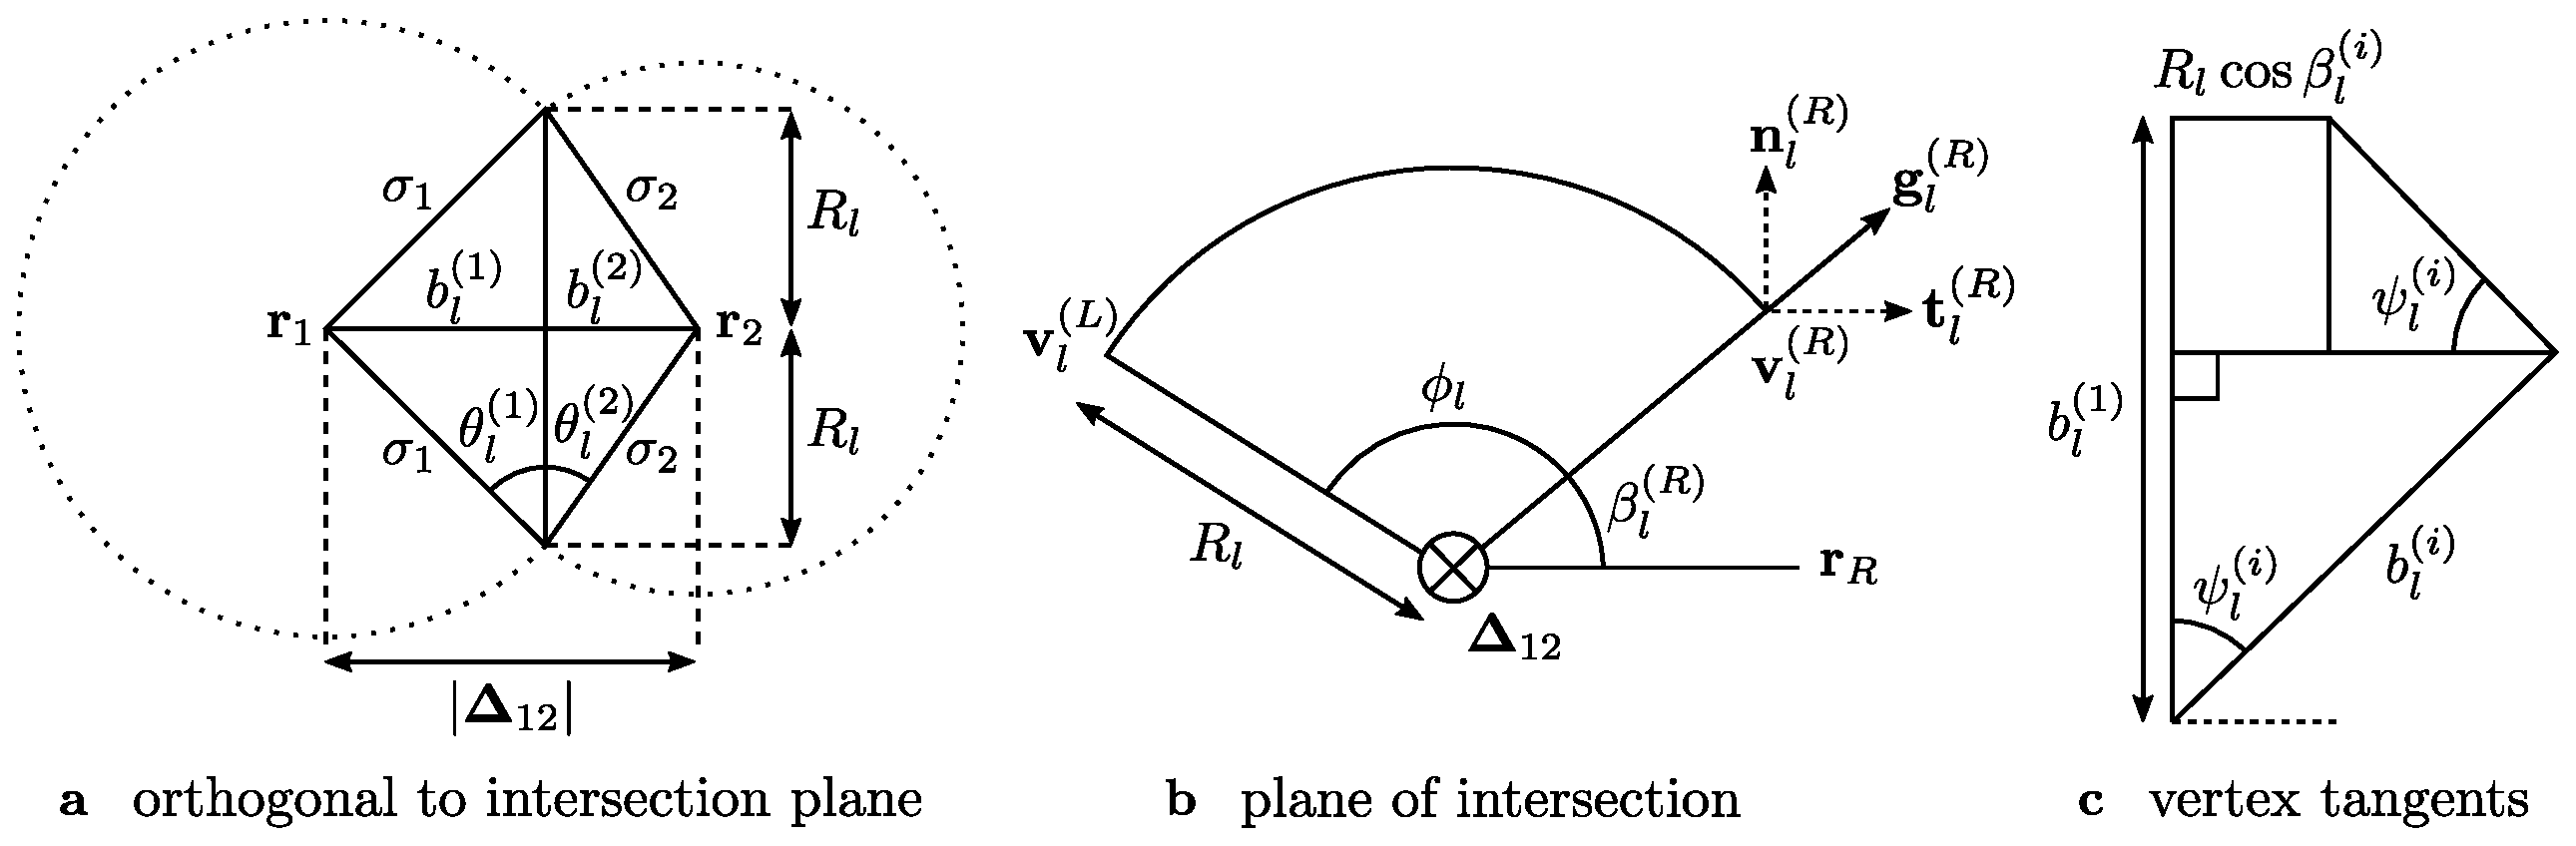
\includegraphics[width=\linewidth,outer]{curvature-geometry}
  \caption{Geometrical quantities involved in the calculation of line curvatures.}
  \label{fig:curvature-geometry}
\end{SCfigure}

\subsection{Particle separations}

The separation between two particle centers is
\begin{equation}
  \vec{\Delta}_{ij} = \vec{r}_i - \vec{r}_j
\end{equation}
which differentiates to
\begin{equation}
  \frac{\partial |\vec{\Delta}_{ij}|}{\partial r_k^\alpha} =
  \frac{r_i^\alpha - r_j^\alpha}{|\vec{\Delta}_{ij}|} (\delta_{ki} - \delta_{kj})
\end{equation}
where $\delta_{ij}$ is the Kronecker delta.

The basis vector for separations differentiates as
\begin{equation}
  \frac{\partial}{\partial r_k^\alpha}
  \left( \frac{\vec{\Delta}_{ij}}{|\vec{\Delta}_{ij}|} \right) =
  \frac{(\delta_{ki} - \delta_{kj}) \vec{e}_k^\alpha}{|\vec{\Delta}_{ij}|}
  - \frac{\vec{\Delta}_{ij}}{|\vec{\Delta}_{ij}|^2}
  \frac{\partial |\vec{\Delta}_{ij}|}{\partial r_k^\alpha}.
\end{equation}

\subsection{Quantities in the plane orthogonal to intersection}

We will label the particles whose intersection creates the circle of arc as 1 and 2 for convenience.
We consider the distances from these particles to the center of the circle as $b_l^{(1)}$ and $b_l^{(2)}$, see Fig.\ \ref{fig:curvature-geometry}(a).
Clearly $|\vec{\Delta}_{12}| = b_l^{(1)} + b_l^{(2)}$.
These distances form equilateral triangles with circle radius $R_l$ of hypotenuse $\sigma_i$ for $i \in \{1,2\}$.
This geometry is sketched in Fig.\ \ref{fig:curvature-geometry}a.
By Pythagoras' theorem we find the unknown distances as
\begin{align}
  R_l
  = \sigma_1 \, \cos{\theta_l^{(1)}}
  = \sigma_2 \, \cos{\theta_l^{(2)}}
  &= \frac{1}{2} \sqrt{
      2(\sigma_1^2 + \sigma_2^2) - |\vec{\Delta}_{12}|^2 -
      \left( \frac{\sigma_1^2 - \sigma_2^2}{|\vec{\Delta}_{12}|} \right)^2
    }, \\
  b_l^{(1)} = \sigma_1 \sin{\theta_l^{(1)}} &=
  \frac{ |\vec{\Delta}_{12}| + \frac{\sigma_1^2 - \sigma_2^2}{|\vec{\Delta}_{12}|} }{2}, \\
  b_l^{(2)} = \sigma_2 \sin{\theta_l^{(2)}} &=
  \frac{ |\vec{\Delta}_{12}| - \frac{\sigma_1^2 - \sigma_2^2}{|\vec{\Delta}_{12}|} }{2}.
\end{align}
The gradients of the angles between the planes are
\begin{subequations}
\begin{align}
  \frac{\partial \theta_l^{(1)}}{\partial r_i^\alpha} &=
  \frac{ 1 - \frac{\sigma_1^2 - \sigma_2^2}{|\vec{\Delta}_{12}|^2} }{2R_l}
  \frac{\partial |\vec{\Delta}_{12}|}{\partial r_i^\alpha}, \\
  \frac{\partial \theta_l^{(2)}}{\partial r_i^\alpha} &=
  \frac{ 1 + \frac{\sigma_1^2 - \sigma_2^2}{|\vec{\Delta}_{12}|^2} }{2R_l}
  \frac{\partial |\vec{\Delta}_{12}|}{\partial r_i^\alpha},
\end{align}
\end{subequations}
and the gradients of the distances are
\begin{subequations}
\begin{align}
  \frac{\partial R_l}{\partial r_i^\alpha} &=
  \frac{|\vec{\Delta}_{12}|}{4R_l}
  \left(
  \left( \frac{\sigma_1^2 - \sigma_2^2}{|\vec{\Delta}_{12}|} \right)^2 - 1 \right)
  \frac{\partial |\vec{\Delta}_{12}|}{\partial r_i^\alpha}, \\
  \frac{\partial b_l^{(1)}}{\partial r_i^\alpha} &=
  \frac{ 1 - \frac{\sigma_1^2 - \sigma_2^2}{|\vec{\Delta}_{12}|^2} }{2}
  \frac{\partial |\vec{\Delta}_{12}|}{\partial r_i^\alpha}, \\
  \frac{\partial b_l^{(2)}}{\partial r_i^\alpha} &=
  \frac{ 1 + \frac{\sigma_1^2 - \sigma_2^2}{|\vec{\Delta}_{12}|^2} }{2}
  \frac{\partial |\vec{\Delta}_{12}|}{\partial r_i^\alpha}.
\end{align}
\end{subequations}
As we must calculate the angles $\theta_l^{(1)}$ and $\theta_l^{(2)}$ and their derivatives for the curvature calculation, i.e.\ Eqs.\ \eqref{eq:integrated-curvature} and \eqref{eq:line-curvature-differential}, a convenient form for these latter derivatives is
\begin{subequations}
\begin{align}
  \frac{\partial R_l}{\partial r_i^\alpha} &
  = - b_l^{(1)} \frac{\partial\theta_l^{(1)}}{\partial r_i^\alpha}
  = - b_l^{(2)} \frac{\partial\theta_l^{(2)}}{\partial r_i^\alpha}, \\
  \frac{\partial b_l^{(1)}}{\partial r_i^\alpha} &=
  R_l \frac{\partial\theta_l^{(1)}}{\partial r_i^\alpha}, \\
  \frac{\partial b_l^{(2)}}{\partial r_i^\alpha} &=
  R_l \frac{\partial\theta_l^{(2)}}{\partial r_i^\alpha}.
\end{align}
\end{subequations}

The expressions in this section are the only quantities which explicitly depend on the sizes of the spheres $\sigma_i$, so we see how it is straightforward to consider the more general surface composed of arbitrarily sized spheres.
The above formulas are simplified if spheres are of equal sizes i.e.\ $\sigma_i = \sigma$ (as in the main text) leading to vanishing of $\sigma_1^2 - \sigma_2^2$ terms.

\subsection{Angular length}

To complete the derivatives in \eqref{eq:line-curvature-differential} we need an explicit expression for the gradient of the angular separation $\phi_l$.
In general, the line consists of an arc along a circle of radius $R_l$, which terminates at the vertices.
%It is possible for lines to not terminate at vertices, however we do not need to consider this special case as it occurs where $\phi_l = 2\pi$ is a constant so the gradient is zero and can be ignored.

We consider the 2d plane containing the intersection $S_1 \cap S_2$.
The center of the intersection circle is
\begin{equation}
  \vec{c}_l
  = \vec{r}_1 + b_l^{(1)} \frac{\vec{\Delta}_{12}}{|\vec{\Delta}_{12}|}
  = \vec{r}_2 - b_l^{(2)} \frac{\vec{\Delta}_{12}}{|\vec{\Delta}_{12}|}.
\end{equation}
The plane of intersection is seen by looking along $\vec{\Delta}_{12}$, making the arc $\phi_l R_l$ perfectly circular, shown in Fig.\ \ref{fig:curvature-geometry}b.
By convention we choose the arc to be a clockwise migration from a `left' vertex to a `right' vertex, which we label $v_l^{(L)}$ and $v_l^{(R)}$ accordingly.
These vertices form at 3-particle intersections, so we will use the suffixes $L$ and $R$ to indicate the 3rd particle index (distinct from 1 and 2) where appropriate.
We write the vertex coordinates as
\begin{equation}
  \vec{v}_l^{(i)} = \vec{c}_l + R_l \, \vec{g}_l^{(i)} \qquad i \in \{L,R\},
\end{equation}
where the unit vectors are
\begin{equation}
  \vec{g}_l^{(i)} =
  \frac
  {\vec{v}_l^{(i)} - \vec{c}_l}
  {|\vec{v}_l^{(i)} - \vec{c}_l|}
  \qquad i \in \{L,R\}.
\end{equation}
The unit vectors for the `right' component are sketched in Fig.\ \ref{fig:curvature-geometry}b.
The central angle is thus defined as the angle (going clockwise) between these unit vectors, i.e.
\begin{equation}
  \cos{\phi_l} = \vec{g}_l^{(L)} \cdot \vec{g}_l^{(R)},
\end{equation}
which after differentiation gives
\begin{equation}
  \frac{\partial \phi_l}{\partial r_i^\alpha} =
  - \frac
  {\frac{\partial \vec{g}_l^{(L)}}{\partial r_i^\alpha} \cdot \vec{g}_l^{(R)} +
   \vec{g}_l^{(L)} \cdot \frac{\partial \vec{g}_l^{(R)}}{\partial r_i^\alpha}}
  {\sin{\phi_l}}.
\end{equation}
So we need explicit expressions for vectors $\vec{g}_l^{(L)}$ and $\vec{g}_l^{(R)}$ and their derivatives to proceed.

We decompose the vertex unit vectors into the following Cartesian basis:
\begin{equation}\label{eq:vertex-unit-vector}
  \vec{g}_l^{(i)} =
  \cos{\beta_l^{(i)}} \, \vec{t}_l^{(i)} + \sin{\beta_l^{(i)}} \, \vec{n}_l^{(i)}
  \qquad i \in \{L,R\},
\end{equation}
where $\vec{t}_l^{(i)}$ is the vector tangent to the plane spanned by particles $\{1,2,i\}$ and $\vec{n}_l^{(i)}$ is normal to this plane.
If $\psi_l^{(i)}$ is the angle $\angle 1i2$, that is
\begin{equation}\label{eq:cos-psi}
  \cos{\psi_l^{(i)}} =
  \frac{\vec{\Delta}_{12} \cdot \vec{\Delta}_{1i}}
  {|\vec{\Delta}_{12}||\vec{\Delta}_{1i}|}
  \qquad i \in \{L,R\}
\end{equation}
then these basis vectors take the form
\begin{subequations}\label{eq:vertex-unit-vector-basis}
\begin{align}
  \vec{n}_l^{(L)} &=
  %\frac{\vec{e}_c \times \vec{e}_l}{|\vec{e}_c \times \vec{e}_l|} =
  \frac{1}{\sin{\psi_l^{(L)}}}
  \frac{\vec{\Delta}_{12} \times \vec{\Delta}_{1L}}
  {|\vec{\Delta}_{12}||\vec{\Delta}_{1L}|}, \\
  \vec{n}_l^{(R)} &=
  %\frac{\vec{e}_r \times \vec{e}_c}{|\vec{e}_r \times \vec{e}_c|} =
  \frac{1}{\sin{\psi_l^{(R)}}}
  \frac{\vec{\Delta}_{1R} \times \vec{\Delta}_{12}}
  {|\vec{\Delta}_{1R}||\vec{\Delta}_{12}|}, \\
  \vec{t}_l^{(L)} &=
  \frac{\vec{n}_l^{(L)} \times \vec{\Delta}_{12}}{|\vec{\Delta}_{12}|}, \\
  \vec{t}_l^{(R)} &=
  \frac{\vec{\Delta}_{12} \times \vec{n}_l^{(R)}}{|\vec{\Delta}_{12}|}.
\end{align}
\end{subequations}
Finally, from Fig.\ \ref{fig:curvature-geometry}c we have
\begin{equation}
  b_l^{(i)} \sin{\beta_l^{(i)}} - R_l \cos{\beta_l^{(i)}}
  = \frac{b_l^{(1)} - b_l^{(i)} \cos{\psi_l^{(i)}}}{\tan{\psi_l^{(i)}}}
  \qquad i \in \{L,R\},
\end{equation}
giving
\begin{equation}\label{eq:cos-beta}
  \vec{g}_l^{(i)} \cdot \vec{t}_l^{(i)} = \cos{\beta_l^{(i)}} =
  \frac{1}{R_l} \left(
    b_l^{(i)} \sin{\psi_l^{(i)}}
    + \frac{b_l^{(i)} \cos{\psi_l^{(i)}} - b_l^{(1)}}{\tan{\psi_l^{(i)}}}
  \right)
  \qquad i \in \{L,R\}.
\end{equation}

With explicit expressions for all of the vectors involved in the arc, the only remaining step is to differentiate.
First, we differentiate the vertex unit vectors Eq.\ \eqref{eq:vertex-unit-vector} in the basis defined by Eq.\ \eqref{eq:vertex-unit-vector-basis} to obtain
\begin{equation}
  \frac{\partial \vec{g}_l^{(j)}}{\partial r_i^\alpha} =
  \frac{\vec{g}_l^{(j)} \times \vec{\Delta}_{12}}{|\vec{\Delta}_{12}|} \,
  \frac{\partial \beta_l^{(j)}}{\partial r_i^\alpha} +
  \cos{\beta_l^{(j)}} \,
  \frac{\partial \vec{t}_l^{(j)}}{\partial r_i^\alpha} +
  \sin{\beta_l^{(j)}} \,
  \frac{\partial \vec{n}_l^{(j)}}{\partial r_i^\alpha}
  \qquad j \in \{L,R\}.
\end{equation}
Second, we take the derivatives of the basis vectors themselves Eq.\ \eqref{eq:vertex-unit-vector-basis} giving
\begin{subequations}
\begin{align}
  \frac{\partial \vec{n}_l^{(L)}}{\partial r_i^\alpha} &=
  \frac{\vec{e}_{c,j} \times \vec{e}_l + \vec{e}_c \times \vec{e}_{l,j}}{\sin{\psi_l}}
  - \frac{\cos{\psi_l}}{\sin{\psi_l}} \psi_{l,j} \, \vec{n}_l, \\
  \frac{\partial \vec{n}_l^{(R)}}{\partial r_i^\alpha} &=
  \frac{\vec{e}_{r,j} \times \vec{e}_c + \vec{e}_r \times \vec{e}_{c,j}}{\sin{\psi_r}}
  - \frac{\cos{\psi_r}}{\sin{\psi_r}} \psi_{r,j} \, \vec{n}_r,
\end{align}
\end{subequations}
Finally, we differentiate the angles from Eqs. \eqref{eq:cos-psi} and \eqref{eq:cos-beta} to get
\begin{subequations}
\begin{align}
 \frac{\partial \beta_l^{(j)}}{\partial r_i^\alpha} &=
  \frac{
  \frac{\partial R_l}{\partial r_i^\alpha}
  \cos{\beta_l^{(j)}} -
  \frac{\partial}{\partial r_i^\alpha}
  \left( R_l \cos{\beta_l^{(j)}} \right)}
  {R_l \sin{\beta_l^{(j)}}}, \\
 \frac{\partial}{\partial r_i^\alpha}
  \left( R_l \cos{\beta_l^{(j)}} \right) &=
  \frac{1}{\sin{\psi_l^{(j)}}}
  \frac{\partial b_l^{(j)}}{\partial r_i^\alpha}
  - \frac{1}{\tan{\psi_l^{(j)}}}
  \frac{\partial b_l^{(1)}}{\partial r_i^\alpha}
  - \frac{b_l^{(j)} \cos{\psi_l^{(j)}} - b_l^{(1)}}
  {\sin^2{\psi_l^{(j)}}}
  \frac{\partial \psi_l^{(j)}}{\partial r_i^\alpha}, \\
  \frac{\partial \psi_l^{(j)}}{\partial r_i^\alpha} =
  -\frac{1}{\sin\psi_l^{(j)}} \frac{\partial(\cos{\psi_l^{(j)}})}{\partial r_i^\alpha} &=
  -\frac{1}{\sin\psi_l^{(j)}}
  \left(
  \frac{\partial}{\partial r_i^\alpha}
  \left( \frac{\vec{\Delta}_{12}}{|\vec{\Delta}_{12}|} \right) \cdot
  \frac{\vec{\Delta}_{1j}}{|\vec{\Delta}_{1j}|}
  +
  \frac{\vec{\Delta}_{12}}{|\vec{\Delta}_{12}|} \cdot
  \frac{\partial}{\partial r_i^\alpha}
  \left( \frac{\vec{\Delta}_{1j}}{|\vec{\Delta}_{1j}|} \right)
  \right),
\end{align}
\end{subequations}
for $j \in \{L,R\}$ in each expression.

\section{Integrated Gaussian curvature}

$\partial\mathcal{L}$ forms a closed two-dimensional surface, so by the Gauss-Bonnet theorem \footnote{\url{https://www.encyclopediaofmath.org/index.php/Gauss-Bonnet_theorem}} the integrated Gaussian curvature must be
\begin{equation}\label{eq:gauss-bonnet}
  X_{\partial\mathcal{L}} = 2\pi \chi
\end{equation}
where $\chi$ is the Euler characteristic of $\partial\mathcal{L}$, a topological constant of the surface.
Thus, the derivative of $X$ is zero everywhere except at pathological points where a topological change in the surface occurs.
In practice this happens when a cavity larger than a particle size forms inside the structure, or when a particle dissociates; being interested in \emph{compact} local structures, we can exclude both of these scenarios from consideration.
Thus, for all local structures $\chi=2$, and the gradient of $X$ is zero everywhere.

Under the above assumptions we do not need to compute $X_{\partial\mathcal{L}}$, but nevertheless it is convenient to do so in order to check the correctness of the algorithm:
\begin{equation}
  X_{\partial\mathcal{L}} =
  -\sum_{l \in L} \phi_l (\sin{\theta_l^{(1)}} + \sin{\theta_l^{(2)}}) +
  \sum_{(i,j,k) \in V} \Omega_{ijk}
\end{equation}
where $\Omega_{ijk}$ is the solid angle spanned by the 3-vectors at vertex $S_i \cap S_j \cap S_k$ \cite{MeckeAA1994}.
The condition that this sum must produce the same result as \eqref{eq:gauss-bonnet} provides a useful check of the numerics.

\section{Intersections of more bodies: possible caveats with quenched geometries}
\label{sec:higher-order-intersections}

A common task with computer simulations is to quench a geometry to find the minimal (or \emph{inherent}) energy structure.
Quenched geometries are inherently athermal so the argument above that intersections of $n>d$ spheres should occur with vanishing probability does not apply; it is common to find intersections of 4 or more particles at the surface in $d=3$ \emph{after a quench}.
To investigate quenched geometries one must properly treat such intersections, as we will demonstrate below with an illustrative example.

An example of these intersections in $d=3$ occurs where 4 particles are arranged in a perfect square (as in e.g.\ any outer face of the body-centered cubic unit cell).
This special geometry corresponds to a bifurcation point in configuration space, where two pairs of surface vertices are simultaneously created and annihilated.
The gradient is not continuous at these points \emph{with respect to the atomic coordinates}, as the continuity of the morphological free energy is only guaranteed with respect to the set $\mathcal{L}$ according to the Hausdorff metric.
In atomic coordinates derivatives can contain poles and step discontinuities.

As the example above illustrates, the gradient is not well defined at pathological points where many spheres intersect.
It is thus impossible to quench these geometries using standard algorithms (which assume smooth functions) and perturbation theories (e.g.\ the harmonic approximation for the free energy) will fail.
A proper treatment of these cases would be required for an investigation of quenched geometries.
In this work we have avoided these considerations primarily by restricting ourselves to geometries thermalised using a Monte-Carlo algorithm (Figures \ref{fig:structure-populations} and \ref{fig:reaction} in the main text).
Construction of the reaction path of $n=6$ particles necessitates an analytic method which uses a quenched geometry, however the geometries for $n=6$ are not pathological so no special consideration is needed.

\ifdefined\includebibliography
  \printbibliography
\fi

\end{document}

\end{appendices}

\printbibliography[heading=bibintoc]

\end{document}
}
\definecolor{bristolred}{RGB}{191,47,56}

\begin{document}

\newgeometry{margin=1in}

%\maketitle
\thispagestyle{empty}
\begin{center}
  \begin{minipage}{0.8\linewidth}
    \centering
    %
\includegraphics[width=0.6\linewidth]{bristol-logo}\par
    %\rule{0.4\linewidth}{0.15\linewidth}\par
    \vspace{3cm}
    %\hline
    {\Large \sc University of Bristol \par}
    \vspace{2cm}
    {\Large \sc Doctoral Thesis \par}
    \vspace{1cm}
    \rule{\textwidth}{0.4pt} \par
    {\LARGE \sc \color{bristolred} Some equilibrium approaches to the high-density liquid (working title) \par}
    \rule{\textwidth}{0.4pt} \par
    %\hline
    \vspace{2cm}
    {\large \it Author:}
    \hfill
    {\large \it Supervisor:} \\
    {\sc \large \href{mailto:joshua.robinson@bristol.ac.uk}{Joshua F.\ Robinson}}
    \hfill
    {\sc \large Prof.\ C.\ P.\ Royall \par}
    \vspace{3.5cm}
   {\large \it A dissertation submitted to the University of Bristol in accordance with the requirements for award of the degree of Doctor of Philosophy in the Faculty of Science, H.\ H.\ Wills Physics Laboratory. \par}
    \vspace{1em}
    {\large August 2019 \par}
  \end{minipage}
  \mbox{}
  \vfill
  \begin{minipage}{0.8\linewidth}
    \raggedleft
    {\large \wordcount words}
  \end{minipage}
\end{center}

\pagenumbering{roman}
\cleardoublepage\chapter*{Abstract}
\addcontentsline{toc}{chapter}{Abstract}

This dissertation describes an investigation into methods for advancing understanding of liquids at high densities, where dynamical processes become highly non-trivial.
Specifically, we address structure in supercooled liquids approaching their glass transition, and the kinetics of nucleating the stable cystal phase.
In both cases we describe the liquid using equilibrium physics, even though the system is metastable and not strictly in equilibrium.
The first three results chapters focus on the supercooled liquid, while the final results chapter addresses nucleation.

In the first part comprising three chapters, we combine geometric techniques with liquid state theory to develop an approach for treating complex many-particle local structures inside the bulk hard sphere liquid.
We introduce the \emph{morphometric approach}, a liquid state theory based on integral geometry, as a means of calculating many-body correlation functions.
We argue for the morphometric approach from several routes, and derive multiple specific theories for hard spheres including one suitable for producing accurate correlation functions.
We later derive the morphometric approach for hard spheres from first-principles using the virial series.
This places the approach on more rigorous ground, and suggests routes to extending the theory as part of a controlled expansion.

With the resulting many-body correlation functions, we are able to predict the concentrations of complex many-particle structures in the bulk liquid; these results are of particular relevance to theories of supercooled liquids and glasses.
We find a bimodality in the energy landscape for hard sphere local structures, where fivefold symmetric structures appear lower in free energy than fourfold symmetric structures.
In addition, we develop similar techniques for predicting the thermodynamic barriers to dynamical processes inside the bulk system.
The solution to the overarching problem of predicting structure formation inside a bulk system has potential to advance study of self-assembly, nucleation and protein folding in aqueous environments.

In a final part we address nucleation of salt crystals in drying aerosol droplets, of particular relevance to climate models and industrial spray drying applications.
Treating the droplet in the continuum limit, we solve the diffusion equation with moving boundary conditions.
By comparison with experimental data we are able to assess the accuracy of classical nucleation theory, with mixed success depending on the system.
%% We find it successfully predicts the nucleation kinetics of \ce{NaCl} aerosol droplets but fails for \ce{NaNO3}.
%% We find a complex interplay between inhomogeneity of the droplet concentration profile and droplet temperature affects the nucleation kinetics.

\cleardoublepage\chapter*{}
\vspace*{0.2\textheight}
\begin{center}
\noindent\emph{Dedicated to all of the cats of the internet, whose rheological properties inspired this delve into liquids.}
\end{center}

\cleardoublepage%\restoregeometry

\chapter*{\vspace{-1em} Acknowledgements}
\addcontentsline{toc}{chapter}{Acknowledgements}

First and foremost, I want to thank my supervisor, Paddy, for being the reason that any of this happened at all, for being a crucial check on my natural impulse to be \emph{too} focused on details and for the fact that I now see beautiful (pink) icosahedra everytime I close my eyes.
I thank him for giving me the freedom to develop my ideas, and for his remarkable degree of patience when that led to me studying six particles for four years.

It has now been several years since Paddy gave me the `humble' task of solving the glass transition once and for all.
Having failed spectacularly at this, I hope we can collectively agree that the real glass transition was the friends we made along the way.
In particular, all of the cave-dwellers (and countless mice) of G.39 who survived the water features, two fumigations and Paddy.
The forces of darkness may have stolen our toaster, but they never broke our spirit%
\footnote{After all, we had the science to do that.}.
I will treasure these memories, and your friendship, until the end of my days.
%Honorable mentions to the contriband toaster and the electric fence of Fowey.
%Together we braved the near-total sunlight deprivation, more mice than I care to remember and an incident with an electric fence.
%Special thanks go out to the electic fence which our trip to cornwall.

I owe a great debt to Francesco Turci for dedicating far more time than I deserve to discuss my work.
I honestly don't think I could have done this without his consistent, valuable input throughout.

I would like to express my gratitude to our collaborator Roland Roth, for founding the Bristol's White Bear institute, conjuring up the initial idea for my project with Paddy and providing guidance along the way.
Additionally, I am deeply grateful to our collaborators in chemistry for what turned out to be a fun and fruitful project: Flo Gregson, Rachel Miles and Jonathan Reid.
I especially thank Flo for doing the experiments which made this collaboration possible, and for providing valuable feedback on my initial attempts at describing them in chapter \ref{chapter:aerosols}.

Special thanks go out to Bob Evans, who showed interest in my work from the very beginning, for the many stimulating discussions about liquid state theory over the years.
I must also thank him for the constructive feedback he gave on an early draft of the paper underlying parts of chapters \ref{chapter:morphometric-framework} and \ref{chapter:morphometric-applications}.
I recall he described me as ``completely mad'' afterwards, which I \emph{think} was a compliment, so I must additionally thank him for inadverently suggesting an `insanity defence' to rely upon in my viva.

I am very grateful to the organisers and lecturers at the Boulder School in Condensed Matter and Materials Physics 2017.
This school influenced my development as a statisical physicist in a myriad of ways.
Notably, I found myself referring back to the phenomenological lectures by Gilles Tarjus while writing chapter \ref{chapter:glass}.

Financially, I acknowledge the European Research Council under the FP7 / ERC Grant Agreement No.\ 617266 ``NANOPRS'' and Paddy for finding ways to support me after this ran out.

I have learned that research is an almost constant uphill struggle, with the occasional false summit.
My most heartfelt appreciation goes out to all my friends and colleagues who made the struggle worthwhile.
I would particularly like to thank Kate Oliver, Nick Wood and Max Meissner for keeping me sane in difficult times, and Kirsty Wynne for teaching me perspective and the meaning of a `false summit'.
Last, and certainly not least, I owe my deepest gratitude to all the close friends and family members who were there for me every step along the way.

%\newgeometry{margin=1in}

\cleardoublepage\chapter*{Declaration}
I declare that..

\cleardoublepage\chapter*{}
\vspace*{0.2\textheight}
\begin{center}
\noindent\enquote{\itshape Keep cool, never freeze.}\hspace{1.5cm} \bigbreak

\hspace{1.5cm} -- Hellmann's\textsuperscript{\textregistered} mayonnaise bottle.
\end{center}


\cleardoublepage\tableofcontents
\cleardoublepage\listoffigures
\cleardoublepage\listoftodos

\restoregeometry

\pagenumbering{arabic}
\setcounter{page}{1}
%TC: macro \marginfootnote [other]
%TC: envir SCfigure [] other
%TC: macrocount beginSCfigure [figure]
\documentclass[11pt,twoside]{report}
\usepackage{preamble}
\setcounter{chapter}{0}
\graphicspath{{../img/}}
\def\includebibliography{}

\begin{document}
\chapter{Introduction}
\epigraph{Everything starts somewhere, though many physicists disagree.}{Terry Pratchett, \emph{Hogfather}, (1996).}

\section{Overview}

%Begin with a short (1–2 pages) broader introduction for a general audience: one that my mother could understand so she knows what I’ve been working on all these years.

What precisely is covered by soft matter, and how to properly demarcate, is a matter of some academic debate.
In some sense soft matter can be most easily understood by : it is the science of ``squishy'' things.
The eminent soft matter physicist Wilson Poon describes soft matter as ``liquids with bits'' in them.
A more precise and scientific definition posits that the energy scale is subject to thermal fluctuations.
So e.g.\ chemical bonds break and reform allowing flow, but the physical processes may be arbitrarily more complex than simple liquids.

Soft matter was clearly preceded by liquids, and it is up to the individual whether liquids should be considered as the antecedent to or subsumed by soft matter.
My personal bias is that liquids represent a subset of soft matter, the zeroth order approximation to real systems.

\section{Simple liquids}

Physics is filled with toy models.
The Ising model is the most widely studied magnetic model, and the usual starting point for students learning statistical mechanics/phase transitions particular the critical point where this is \emph{the} model system.

What are simple liquids, with hard spheres at the forefront.
\hl{Hard spheres serve as a good touchstone for some of the fundamental knowns and controversies in liquid state theory and, by extension, soft matter.}
The physicists favourite toy model is the hard sphere liquid.
Interaction potential is the no-overlap condition%
\marginfootnote{I like to imagine them as ideal billiard balls, i.e.\ without any dissipative forces like friction so they continue to bounce off one another forever.}:
\begin{equation}
  U =
  \begin{cases}
    \infty & \; r < \sigma \\
    0 & \; \textrm{otherwise}.
  \end{cases}
\end{equation}
As the potential is everywhere zero or divergent, temperature has no effect on the interactions making this system athermal.
Instead, the natural control parameter is (number) density $\rho = N/V$, or as it is normally rescaled into volume fraction: the volume of space occupied by the spheres i.e.\
\begin{equation}
  \eta = \frac{N v}{V} = \rho v
\end{equation}
where $v$ is the volume of a single hard sphere.

When van der Waals wrote down their famous equation of state for real gases, i.e.\
\begin{equation}
  (p - a N)(V - Nv) = N k_B T
\end{equation}
where $V - Nv$ corrects for the volume occupied by finite-sized particles and $p - aN$ for the interactions,
it was widely believed that to go beyond this to understand liquids more sophisticated treatments of the \emph{attractions} would be required.
History shows that in actual fact the treatment of \emph{repulsions} were lacking.
It turns out that to a large degree simple liquids can be considered as hard spheres plus an attractive perturbation: an accurate treatment of the repulsion is needed, attractions can be less accurate.

\begin{SCfigure}
  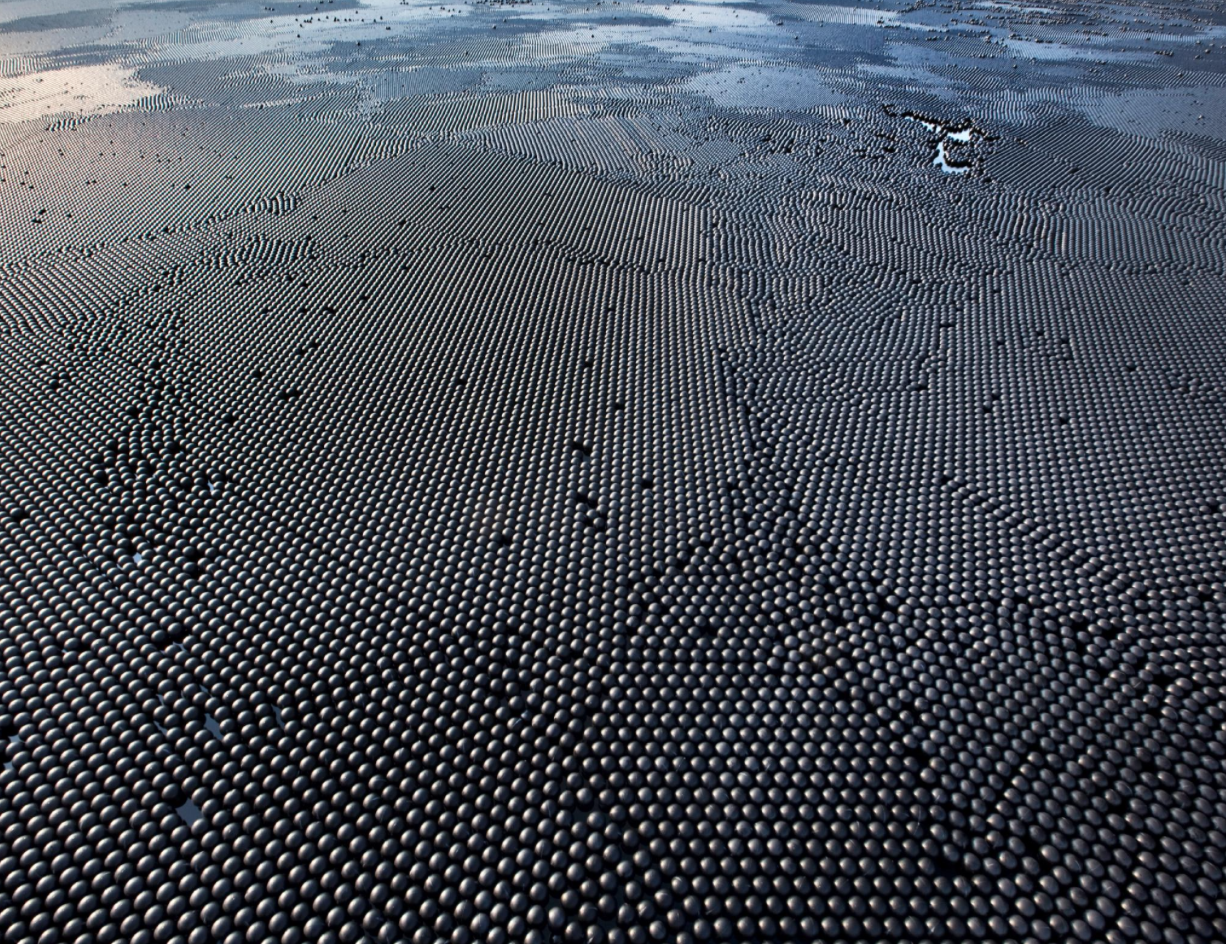
\includegraphics[width=0.75\linewidth,outer]{shade-balls}
  \caption[Shade balls floating on water: a 2d `crystal']{
    Shade balls covering the Los Angeles reservoir to cool water preventing evaporation and certain light-activated chemical reactions at the water surface.
    As macroscopic objects these balls interact as hard spheres, and they spontaneously form long-ranged orientational order seen as hexagonal domains.
    This is reminiscent of crystallisation in atomic systems.
    Image by Gerd Ludwig, \emph{National Geographic} (2007).}
  \label{fig:shade-balls}
\end{SCfigure}

Despite their coarse simplification of real atomic interactions, we see that hard spheres actually capture a lot of the essential physics.
To illustrate this consider the phase diagram of hard spheres Fig.\ \ref{fig:hs-phase-diagram}.
We see there is a freezing transition at $\eta = 0.494$, suggesting that the liquid will spontaneously order into a crystal at high densities.
This is surprising, in everyday scenarios (e.g.\ water) we are used to seeing crystallisation as one lowers temperature and the explanation normally given in classrooms is that the crystal is favoured due to attractions between molecules.
Now, in real systems crystallisation can also be triggered by changes to density also so density being a control parameter is not a problem, however the lack of attractions should, if this intuition were correct, prohibit crystallisation.

It turns out in the case of hard spheres that the crystal has a larger entropy above freezing, so entropy itself triggers crystallisation.
This was a hotly debated topic \cite{?,?,?} until is was solved by computer simulation in \cite{?,?,?} and experiment \cite{?,?,?}.
Part of the reason people could not believe that the crystal is entropically favoured, is because we often mistakenly take entropy to be a measure of disorder when it in fact more complicated.
The crystal might be more ordered than the liquid, with a lower \emph{configurational} entropy, however the entropy includes \emph{all} microstates not just averaged ones: the crystal is compensated by having a much larger \emph{vibrational} entropy than the liquid at high densities.
Including both these contributions leads to the phase diagram that we know today.

A similar effect is seen in balls floating on water as in e.g.\ peas in a saucepan or shade balls covering a reservoir.
The hard interactions between the balls causes%
\marginfootnote{In an attempt to find an everyday example, I have taken liberties with the interaction being purely hard; I suspect that floating balls feature effective attractions due to \emph{hydrodynamic} interactions at the water surface.}[-3cm]
them to `crystallise' at high densities as seen in Fig.\ \ref{fig:shade-balls}..
Strictly speaking these are not crystals in the sense of long-range \emph{translational} order, instead they are said to possess long-range \emph{orientational} order.
This subtlety emerges because the floating balls are confined to the water surface making them effectively two dimensional; fluctuations are strong enough in two dimensions to overcome truly long-ranged positional ordering \cite{MerminPRL1966,MerminPR1968}.

We have extolled the virtues of hard spheres, however this should not be interpretted as saying that this model system capture \emph{all} of the physics of real systems: it is a toy system after all.
They are merely a very good starting point for more complex systems.
As an example of physics they do \emph{not} capture, consider the critical point of real liquids.
Liquid-gas critical phenomena emerges from a competition between attractive and repulsive forces, with divergent fluctuations at the critical point.
It is thus impossible for a system with purely repulsive interactions, like hard spheres, to feature a critical point.
That being said, many theories predict critical phenomena quite well by taking a hard sphere potential and incorporating a mean-field like attractive perturbation \cite{?} so a hard sphere system provides a good reference point.

Hard spheres exist in more than just a theorist's imagination: they can be experimentally realised in colloidal experiments.
Colloidal suspensions are mixtures of solute immersed in a solvent composed of much smaller particles.
Colloidal particles are typically at the micron-scale.
These typically feature complex interactions \cite{Royall?,?,?} however these can be tailored to closely approximate hard sphere like interactions through steric stabilisation.
\todo{What is an aerosol? What is a dispersion?}
Colloidal experiments closely match hard simulations and theoretical predicitons \cite{?}.
Notably one can determine the phase diagram see Fig.\ \ref{fig:hs-phase-diagram}.
Note the glass at very high densities.

\begin{SCfigure}
  \missingfigure[figwidth=\linewidth]{}%
  \caption[The hard sphere phase diagram]{
    The hard sphere phase diagram, including the metastable branch.
    a: theoretical phase diagram.
    b: experiments, including the glass (image reproduced from \cite{?}).
    This is one of the most iconic images in the field, and no discussion of colloidal hard spheres would be complete without it.}
  \label{fig:hs-phase-diagram}
\end{SCfigure}

\begin{SCfigure}
  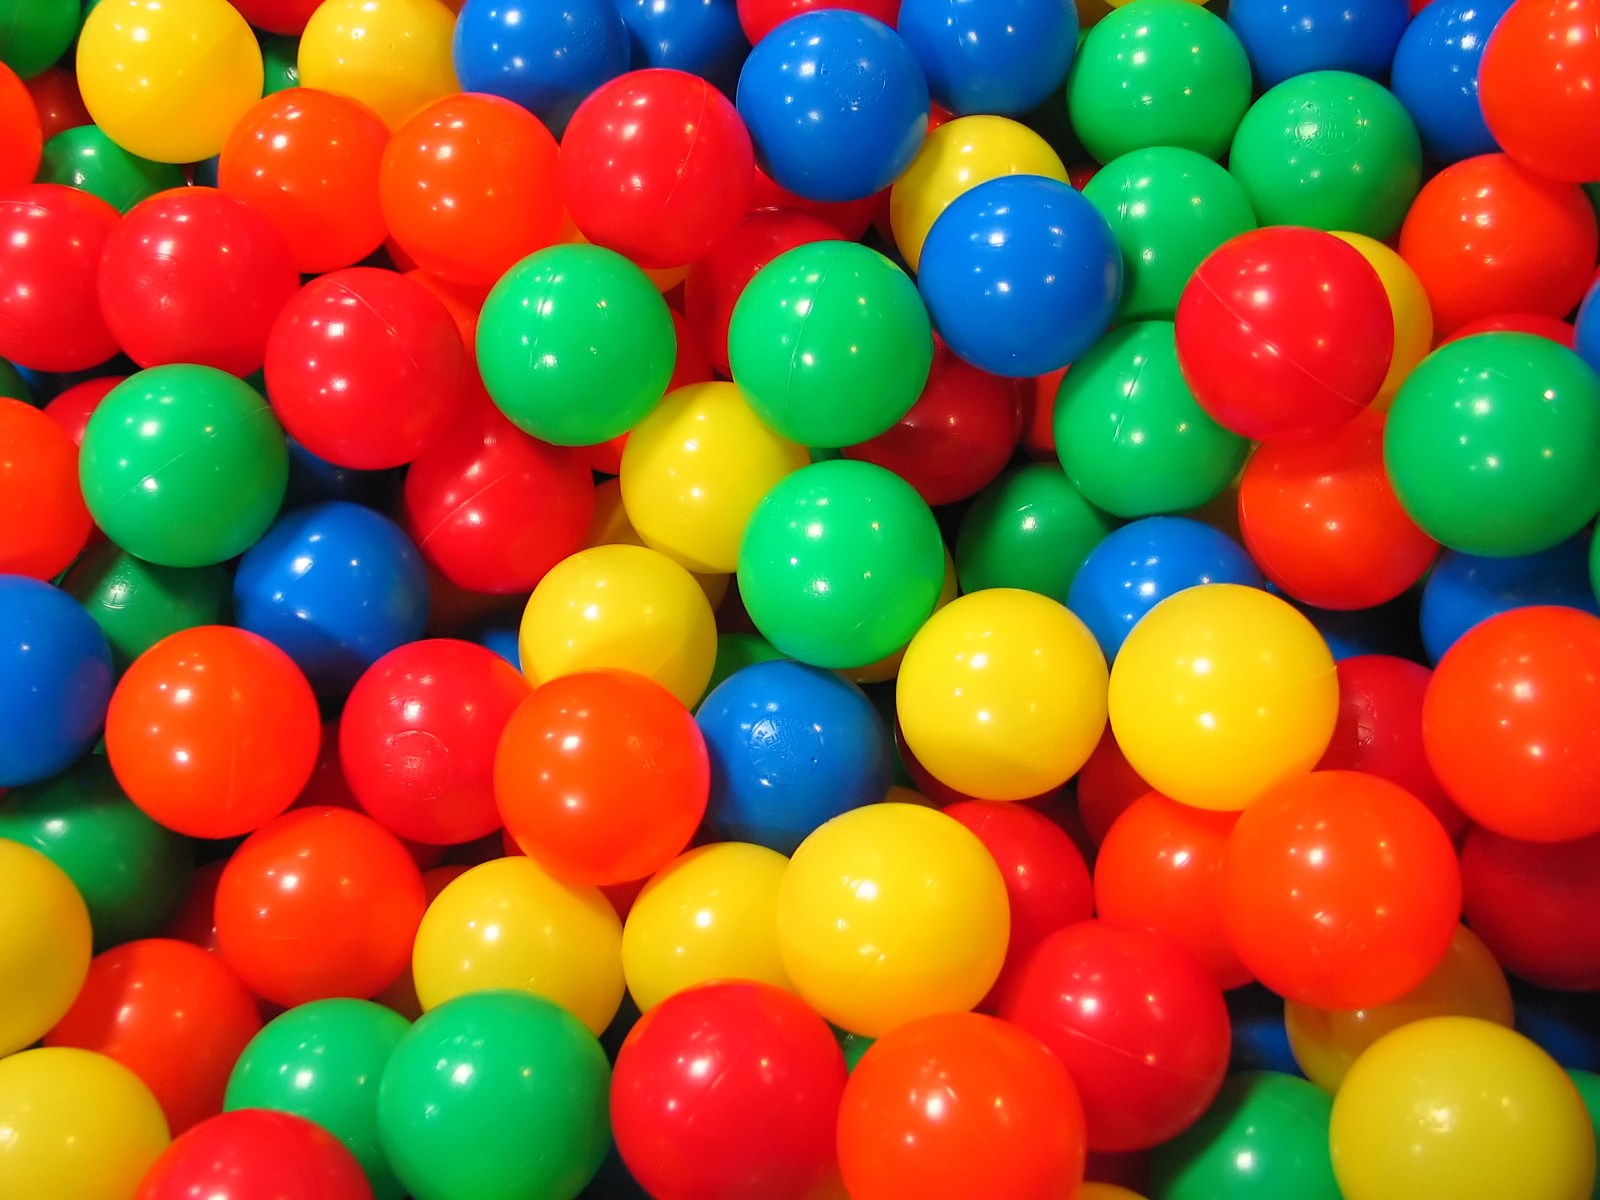
\includegraphics[width=0.75\linewidth,outer]{ball-pit-horizontal}
  \caption[Random close packing in a ball pit]{
    Random close packing of hard spheres in a ball bit.
    Image by Peter Ong.}
  \label{fig:rcp}
\end{SCfigure}

As the most widely studied model interaction potential we know a lot about its equilibrium structure (phase diagram) in bulk and even inhomogeneous thanks to density functional theory \cite{?,?,?}.
However, its behaviour off-equilibrium at high densities is hotly debated.
The two biggest unresolved research topics for this subject:
\begin{itemize}
\item \emph{Nucleation}: given that above freezing the crystal ? Theoretically predicted nucleation rates from simulation studies differ by 12 orders of magnitudes from experiments, purported to be the second biggest disagreement between theory and experiment in all of science \cite{?}.
\item \emph{Metastable liquid}: if one could avoid crystallisation and equilibrate only over the liquid microstates, what would be the ultimate fate of the liquid?
  We will talk more about this in \ref{?}.
\end{itemize}

There is a deep connection between hard spheres and computer science.
Packing problems have been studied \cite{Cohn,Conway,Sloane} and they are notoriously difficult; Kepler conjectured the optimal packing in 3d was the face-centred cubic/hexagonal close packing but it took 300(?check) years to solve this.
The final proof was computer aided, and not simple.
Packing problems are connected with encoding/encryption.
Transmitting a signal requires a way to encode a message across a band(?): if packed too tightly on the band(?) then noise will destroy the signal to it is desirable to optimise the sites for bits \cite{Cohn,?,?}.
Additionally, lattice based encryption techniques are one of the alternatives to prime factorisation: the coming development of quantum computers \cite{?,?} would render prime factorisation easy because of Shor's algorithm \cite{Shor?} rendering standard encryption techniques insecure.
The techniques developed for the mean field hard sphere problem have been applied to the perceptron model \cite{?}, and deep-learning neural networks which are naturally high dimensional problems lending themselves to a mean field treatment \cite{?}.

\begin{SCfigure}
  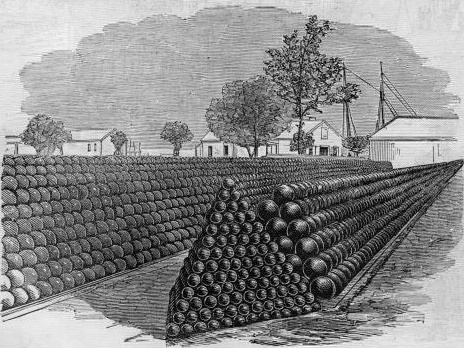
\includegraphics[width=0.75\linewidth,outer]{cannonballs}
  \caption[Close packed cannonballs]{
    Sketch of close-packed stacks of cannonballs in Fortress Monroe.
    Image by Stacy, \emph{Harper's weekly} (1861)}
  \label{fig:fcc}
\end{SCfigure}

Although hard spheres will be our focus, we will mention the importance of systems of hard particles of other shapes for self-assembly.
Self-assembly is an active area of soft matter: it is technologically desirable to tailor the final structure by controlling the building blocks.
Imagine assembling nanomachines or artificial cells by controlling the chemistry.
It is found that varying the size and shape of hard particles can reproduce all the complexity of the periodic table \cite{Glotzer?,Dijkstra?}.
Hard spheres are the simplest such system, so a theory which can treat other geometries is desirable.

The primary goal of this thesis is to advance the methods of treating liquids at high densities, particularly concerning the role of thermodynamics in dynamical arrest and nucleation.
These methods can be readily adapted to more complex systems, such as protein folding in aqueous solution or self-assembly of complex structures.

A secondary goal would be to advance the understanding of the fundamental theory of hard particles in some small way.
I have attempted to develop the geometrical theory behind the methods of Chapters \ref{?} and \ref{?} in a generally applicable way;
I have done this to the best of my ability, but my primary skills lie in numerical methods and I am a second-rate theoretician.

\section{Supercooled liquids and glasses}

It is widely reported that glass is actually liquid, and as evidence of this the thickness of old windows at the bottom is pointed to.
This is actually a matter of some dispute, but contains a grain of truth.
Pre-modern methods of creating window glass involved spinning molten glass on magma to flatten it out.
Centrifugal forces caused the glass to be thicker on the outer disk, so panes of glass would always be heavier in one direction%
\marginfootnote{And personally, if I were setting an uneven pane of glass I would place the heavy part at the bottom.}.

To a soft matter physicist glass is a broader term, referring to a wide class of materials while the window glass of common parlance is referred to by its chemical name \emph{silicate}.
This class of materials share many features of being disordered etc \cite{?} although in some sense they are connected by what they do \emph{not} do: which is flow on human timescales.
When I refer to `glass' I will be using it in this broad technical sense of a state of matter.
Some examples besides silicate:
\begin{itemize}
\item Most of the ice in the universe exists in an amorphous state in comets \cite{?}
\item Ceramics
\item Plastics: amorphous polymers
\end{itemize}
Of more abstract nature which could be called glassy though they are not materials
\begin{itemize}
\item Gels: super glasses, liquid like bit plus a network/backbone which has glassy dynamics
\item Neural networks
\item Non-deterministic polynomial time (NP) problems
\end{itemize}
We will not be directly addressing the latter type of more abstract problems which could be considered glasses, although they are arguably related due to a similar underlying disorder.
We will be focusing on only the most rudimentary of glassy phenomenology: the dynamical arrest of liquids at high densities/low temperatures when crystallisation is avoided.
Especially as it manifests in hard spheres, which as discussed is the reference system of choice for simple liquids.

So what do we mean by dynamical arrest.
Typically we can look at one of two (related) quantities: viscosity or relaxation time.
Viscosity measures how resistant the thing is to flow, while relaxation time measures the typical microscopic time for things to move around i.e.\ liquid like behaviour.
As a practical definition, a glass is defined in the lab as any material for which the relaxation time exceeds 100\ce{s}: this point is called the experimental glass transition.
This is somewhat arbitrary, although the location of the glass transition point is not particularly sensitive to where you set the threshold because of how rapidly the viscosity/times are increasing around there.
\todo{Need: Angell plot, fragile vs strong}

Personally, the observation that got me interested in the field is the entropy argument.
If one compares the difference between the entropy of the crystal and the glass, and extrapolates wildly one expects there to be a point where the glass has a lower entropy than the crystal.
This is not very meaningful by itself, as we have already established by discussing the crystal vibrational entropy can be quite subtle so it is possible for the liquid to have a lower vibrational entropy.
However, if one corrects this with more modern techniques to measure just the entropy corresponding to non-trivial motion we see that there is a point where the configurational (i.e.\ not purely vibrational) entropy vanishes: this would imply the system is frozen in a single configuration.
Such a point would define a transition to a genuine thermodynamic phase, an ideal glass.
\todo{Plots of configurational entropy}

A diverging timescale necessarily requires a diverging point-to-set length scale and a vanishing configurational entropy, a proof given in \cite{?}.
This must trivially occur at the very least $T=0\si{K}$ where relaxation timescales diverges, however much like the lack of a phase transition in the Ising model in $d=1$ this is not a true thermodynamic phase transition because it cannot be crossed.
Recent numerical evidence suggests that a model glassformer in $d=2$ does not show a transition, also vanishing at $T=0\si{K}$ \cite{Berthier?}.
So the central question of glass is what happens in $d=3$, is there a vanishing configurational entropy at a finite $T > 0$ with an accompanying thermodynamic glass transition?
In mean-field, formally in the limit of infinite spatial dimensions $d \to \infty$, the hard sphere system has been shown to have a true transition, however the critical dimensions are unknown so it is unclear what happens in $d=3$ \cite{Parisi,Zamboni,Charbonneau,Kurchan,?,?}.

\todo{Jamming: how does it relate to glass}

\section{Notes from Tarjus}

Overview of the glass transition.
Salient features: why hard, interesting, unique.

What is a glass?
Frozen in a (apparently) disordered state.
All sorts of glasses, structural, spin, orientational, electron, vortex.
Glasses formed by liquids, colloidal suspensions and polymers: traditional structural glasses.
Solid: doesn't flow on observational time, resists small/infinitesimal shear (acts like solid).
Amorphous, apparently amorphous: no periodic arrangement like in crystal.
Homogeneous makes useful for technology: useful for e.g.\ optical properties.

Hard glasses: high elastic constants.
Colloidal suspensions: soft matter version, small elastic constants.
Same phenomenology though.

Cooling a liquid.
Take thermodynamic quantity (e.g.\ volume, entropy, enthalpy): usually crystallise.
(Picture)
First-order transition bypassed by quick cooling.
Enter supercooled liquid phase.
No longer equilibrates/relax/flows, call it a glass: occurs at glass transition.
Glass is a solid for all practical purposes.

SC liquid: same characteristics as at equilibrium.
Independent of preparation: loses memory of initial preparation.
Measureable properties have time translational invariance/are stationary.
Time independence of all observables, i.e.\
\begin{equation}
  \langle A(t) \rangle = \langle A \rangle
\end{equation}
including correlation functions e.g.\
\begin{equation}
  \langle A(t) A(t') \rangle = \langle A(0) A(t - t') \rangle
\end{equation}
(equation for stationary)
Fluctuation-dissipation theorems.
Linear response regime: response to perturbation related to correlation function (spontaneous fluctuations).
\begin{equation}
  \chi_A (t, t')
  =
  - \beta \Theta(t - t')
  \frac{d}{dt}
  \left(
  \bigg\langle
  (A(t) - \langle A \rangle)
  (A(0) - \langle A \rangle)
  \bigg\rangle
  \right)
\end{equation}

\ifdefined\includebibliography
  \printbibliography
\fi
  
\end{document}

%TC: macro \marginfootnote [other]
%TC: envir SCfigure [] other
%TC: macrocount beginSCfigure [figure]
\documentclass[11pt,twoside]{report}
\usepackage{preamble}
\setcounter{chapter}{1}
\graphicspath{{../img/}}
\def\includebibliography{}

\externaldocument{morphometric-framework}

\begin{document}
\chapter{Background}
%\epigraph{It tells me that the Creator used the wrong kind of circles.}{Terry Pratchett, \emph{Pyramids} (1989).}
\epigraph{It was not certain what significance the ceremony held... but the formality was no less sacred for it being unintelligible}{Mervyn Peake, \emph{Titus Groan}, (1946).}

In this chapter we provide a \emph{concise} account of the foundational frameworks underlying the two themes of this thesis: \emph{integral geometry} and \emph{liquid state theory}.
I expect the reader to have a background in statistical physics, so my account of liquid state theory is not intended to be exhaustive; for more in-depth treatments see the references herein.
By contrast, I do \emph{not} expect much familiarity with integral geometry.
Understanding the underlying mathematical detail is not essential to follow the rest of the thesis, so I will focus more on the key concepts and notation than detailed derivation.
I anticipate the expert reader will skim over this chapter, so I have placed the important theorems in boxes as a guide to the most relevant parts.

As many-body correlation functions are a central theme of the results chapters, I have emphasised correlation functions in section \ref{sec:liquid-structure} on liquid structure to the point where I have somewhat belaboured giving the explicit forms and normalisations of the various correlation functions.
Even though we will only use one particular hierarchy of correlation functions in the results chapters, I personally found it helpful to have these formulas in one place.
I have found myself frequently revisiting the transformations between the various hierarchies of correlation functions, so I include them in anticipation that someone repeating or extending this work can profit from having a kind of ``cheat sheet''.

\section[Integral geometry. Or ``How long is a piece of string?'']{Integral geometry\\ {\large Or ``How long is a piece of string?''}}
\label{sec:integral-geometry}

\subsection{Towards a geometric interpretation of extensivity}

Geometry has been a recurring theme in physical theories, appealing because of its intuitive nature.
There are many ways that geometric ideas can be incorporated, but our focus will be on expansions of thermodynamic quantities in terms of \emph{sizes}.
The usefulness of this particular focus is directly connected to the familiar concept of \emph{extensivity} in statistical mechanics, which we will use to guide the following discussion.
Thermodynamic potentials must be extensive to remain well-defined in the thermodynamic limit,
%Defining an extensive quantity as one that scales proportionally to system size, the first meaning of size that comes to mind is probably the volume.
so by focusing on extensive quantities we ensure a thermodynamically consistent description in this limit.

%The first notion of size that likely comes to mind is the volume, though we will generalise to all reasonable notions of size.
%The simplest example we can give is from statistical mechanics: an \emph{extensive variable} is one that scales proportionally to the system volume.
%For a finite system $K \subset \mathbb{R}^d$ %the volume is expressed
%% \begin{equation}
%%   V[K] = \int_K d\vec{r}.
%% \end{equation}
%Then,
As an example, extensive quantities include the \emph{entropy} of a large system which can be expressed in terms of system volume as
\begin{equation*}
  S = s V
\end{equation*}
where $s$ would be an entropy density which is \emph{intensive}, meaning it does not change with system volume.
Another example is the surface energy
\begin{equation*}
  E = \gamma A
\end{equation*}
where $\gamma$ is the surface tension and $A$ is the surface area.
More refined notions define a variable as extensive if it is a \emph{first-order homogeneous function} of any linearly independent set of (different) extensive variables characterising the system size \cite{Chandler1987}.
That is, a variable $\phi$ is extensive if
\begin{equation}\label{eq:extensive-homogeneity}
  \phi(\lambda Y_1, \cdots, \lambda Y_n)
  =
  \lambda \phi(Y_1, \cdots, Y_n)
\end{equation}
where $\{Y_1, \cdots, Y_n\}$ are a complete (linearly independent) set of extensive variables describing the system size.
We will explore what other reasonable notions of `size' there may be, in effect finding a complete set of extensive variables, in the hope that we arrive at ideas which prove useful in developing new theories.

We introduced the area above as a size descriptor for a surface.
Borrowing ideas from differential geometry, we can also characterise the surface's shape through \emph{curvature}.
A surface is a two-dimensional manifold so its local shape is described by two basis vectors.
Supposing the surface is parameterised by coordinates $(x_1, x_2)$, then the basis vectors at a point on the surface $\vec{r}$ are
\begin{equation}
  \vec{e}_\alpha := \frac{\partial \vec{r}}{\partial x_\alpha}
  \qquad \alpha \in \{1, 2\}.
\end{equation}
Then, the shape of the surface is characterised by changes in the basis vectors leading to the curvature tensor
\begin{equation}
  \kappa_{\alpha \beta} := \frac{\partial \vec{e}_\beta}{\partial x_\alpha}
  \qquad \alpha, \beta \in \{1, 2\}.
\end{equation}
The values of the curvature tensor will depend on the choice of coordinate system $(x_1, x_2)$, so it is usual to consider the \emph{curvature invariants}, i.e.\ the trace and determinant%
\marginfootnote{This argument is readily generalised to $(d-1)$-dimensional surfaces in $\mathbb{R}^d$, where we would find $d-1$ invariants of the curvature tensor.},
leading to the the \emph{mean} and \emph{Gaussian curvatures}
\begin{subequations}
  \begin{align}
    H &:= \frac{\Tr{\kappa}}{2}, \\
    G &:= \det{\kappa}.
  \end{align}
\end{subequations}
As an example of how curvature can be a useful concept in statistical mechanics, we put forward the Young-Laplace equation which writes the pressure difference between two fluids as
\begin{equation*}
  \Delta p = 2 \gamma H,
\end{equation*}
with applications to e.g.\ phase coexistence \cite{YoungPTRSL1805,Laplace1805} or frost damage to porous solids \cite{EverettTFS1961}.
Extensive curvature measures are obtained by integrating the curvature invariants over the surface, leading to the integrated mean and Gaussian curvatures $C$ and $X$.

Together, the extensive geometric variables we have introduced so far can be written as%
\marginfootnote{We use the usual physicist abuse of notation where $V$ refers to both a region in space $V \subset \mathbb{R}^3$, and also the physical volume of this space.}
\begin{subequations}\label{eq:intrinsic-volumes-surface-integrals}
  \begin{align}
    \label{eq:volume-measure}
    V
    &=
    \int_V \, d\vec{r},
    \\
    A
    &=
    \int_{\partial V} \, d\vec{r},
    \\
    C
    &=
    \int_{\partial V} H(\vec{r}) \, d\vec{r},
    \\
    X
    &=
    \int_{\partial V} G(\vec{r}) \, d\vec{r}.
  \end{align}
\end{subequations}
The latter three quantities are \emph{expressed} here as the surface integrals, but we shall see that they are really size measures on the volume $V$.
These clearly form a linearly independent set%
\marginfootnote{This can be quickly determined by considering their units, i.e.\ $V: [\si{\metre^3}]$, $A: [\si{\metre^2}]$, $C: [\si{\metre^1}]$, $X: [\si{\metre^0}]$.},
but less obvious is the fact that these are the \emph{only} reasonable notions of size in three-dimensions.
This is a central finding of \emph{integral geometry}, which we will expand on in subsequent sections.
%is a powerful tool for incorporating intuitive, flexible ideas into theories.
%For this reason geometric approaches are common in statistical mechanics such as the Young-Laplace equation, which corrects Asakura-Ozawa
A consequence of this is that together $\{V, A, C, X\}$ form a complete basis for system size in three dimensions, so we could redefine an extensive quantity as one which can be written
\begin{equation}\label{eq:extensive-integral-geometry}
  \phi = a_3 V + a_2 A + a_1 C + a_0 X,
\end{equation}
which, as a linear relation, clearly obeys \eqref{eq:extensive-homogeneity} during the transformation%
\marginfootnote{Note: the rescaling of $\lambda V$ here refers to rescaling the volume measure \eqref{eq:volume-measure}, \emph{not} the object $V \subset \mathbb{R}^3$; in the latter case we would obtain the (non-extensive) transformation $\{V, A, C, X\} \to \{\lambda V, \lambda^{2/3} A, \lambda^{1/3} C, X\}$.}
$\{V, A, C, X\} \to \{\lambda V, \lambda A, \lambda C, \lambda X\}$.

Integral geometry provides elegant and unified description of sizes, and was crucial in the development of modern theories of hard spheres \cite{RosenfeldPRL1989,KonigPRL2004}, including the main ideas underlying chapters \ref{chapter:morphometric-framework}, \ref{chapter:morphometric-applications} and \ref{chapter:resummation}.
This framework thus provides the route to generalising geometrical theories such as the Asakura-Oosawa model for depletion forces \cite{AsakuraJCP1954,AsakuraJPS1958}, and more generally any free volume theory which expresses an energy in terms of a volume in space.
%Integral geometry generalises the underlying geometric principles of these theories into a unified framework for characterising size.
%% We could argue that fundamentally these theories are based on measuring physical sizes.
%% Integral geometry offers a mathematically rigorous formalism for describing sizes, so presents a possible starting point for free volume theories.
%Ideas from this branch of mathematics were crucial to the development of fundamental measure theory (section \ref{sec:fmt}), so it makes sense to place this before the section on liquid state theory.
As integral geometry is generally unfamiliar to people with a background in physics, we will place emphasis on the concepts and intuition rather than rigour and proofs.
We work mainly from standard texts Refs.\ \cite{Santalo2004,SchneiderACIG1984,Schneider2008,Klain1997}.

\subsection{What do we even mean by size?}
\label{sec:what-is-size}

In order to proceed we must define `size', and specify precisely which objects this definition applies to.
We put forward the following qualities of the measures $V, A, C$ and $X$ which make them intuitive notions of size:
\begin{enumerate}
\item They are invariant with respect to translations and rotations, so that an object's size is independent of the observer.
\item They increase additively, i.e.\ they transform under combination of subsystems via the inclusion/exclusion relation e.g.\ for two objects $K_1$ and $K_2$%
  \marginfootnote{We use the square brace notation $V[\cdot]$ to indicate that the size measures are generalised functions, or \emph{functionals}, of their arguments.}
  \begin{equation}\label{eq:additivity}
    V[K_1 \cup K_2] = V[K_1] + V[K_2] - V[K_1 \cap K_2],
  \end{equation}
  and similar expressions for $A$, $C$, and $X$.
  As corollaries, this property contains the idea that the size of nothing is zero, e.g.\ $V[\emptyset] = 0$, and leads to the homogeneity property of extensive variables \eqref{eq:extensive-homogeneity} through \eqref{eq:extensive-integral-geometry}.
\item They are continuous%
  \marginfootnote{Specifically, in integral geometry this continuity property is with respect to the \emph{Hausdorff metric}.
    Details on this can be found in standard texts, e.g.\ Refs.\ \cite{Santalo2004,SchneiderACIG1984,Schneider2008,Klain1997}.}.
  Loosely speaking, this means that the size measures converge as the object is approximated by increasingly finely meshed polyhedra excluding e.g.\ fractal geometries.
  As a simple intuitive example, the measurement of a length will converge continuously to some number as one uses rulers with progressively finer distance markings.
\end{enumerate}
The final property specifically excludes geometries for which we do not expect there to be any reasonable measurement of size.
These properties are the defining characteristics of more general size measures in integral geometry \cite{Santalo2004, Klain1997}.

%% First we define our objects: sets in Euclidean space.

%% We could completely describe the size of simple objects by completely defining their geometry, e.g.\ the dimensions of a box.
%% This is of course sufficient, however it is not very useful.
%% However, this may not be straightforward for more complex objects, and by abstracting the problem somewhat we can obtain useful theorems etc.
%% We now give a brief justification of the above \emph{ansatzes}, in particular why there are only four terms in the expansion.
%% Radius is the only natural parameter for a sphere, however for more general geometries there might be arbitrarily many parameters so one may wonder if they should be included in a general geometric expansion.

Naively, we might attempt to evaluate the size measures on all subsets $V \subset \mathbb{R}^3$, however this turns out to be too broad a definition.
In particular, this leads to the \emph{Banach-Tarski paradox} in which an object can be broken into two, then recomposed through rigid transformations into two objects identical to the original one  \cite{BanachFM1924}; by \eqref{eq:additivity}, a paradox ensues where the original volume is equal to twice itself.
A better definition is the restriction to \emph{polyconvex sets}%
\marginfootnote{The set of polyconvex objects is also sometimes called the \emph{convex ring}.}: objects formed by countable union of \emph{compact} and \emph{convex} objects.
By compact, we mean objects which are
\begin{enumerate}
\item \emph{bounded}, so they must be finite in scope, as no meaningful size can be defined for a body spanning an infinite region of space, and
\item \emph{closed}, so they contain their boundary.
  %, so the surface exists on which measures $\{A,C,X\}$ are defined.
  %This is an important property which we will see by example in discussing the Gauss-Bonnet theorem below.
\end{enumerate}
We write the collection of objects in $d$-dimensions which are compact and convex as $\mathcal{K}^d$.
This class of objects covers most physically relevant geometries, excluding geometries where size measures may be pathological such as those with fractal structures.
%The empty set $\emptyset$ is a compact body, albeit a special case with zero size.
%Compact convex set $K \in \mathcal{K}$ notation.

%% The first intuitive notion for a size: the size of nothing is zero, i.e.:
%% where $\emptyset$ is the empty set.
%% A box: take the largest length, but then the `size' is not increased by modifying its smallest dimensions.
%% Ideally, we want a size measure that increases monotonically as we add additional material. This leads to additivity:
%% \begin{equation}
%%   \phi(A \cup B) = \phi(A) + \phi(B) - \phi(A \cap B)
%% \end{equation}
%% Connection with entropy, leads to homogeneity in arguments which is the building block for extensivity of a thermodynamic potential.
%% This provides a geometrically precise foundation for thermodynamic potentials.

As a way of justifying the above claims, and as a segue into other topics, we introduce a (seemingly) new measure: the \emph{Euler characteristic} $\chi$ which simply counts the number of disjoint objects in a set%
\marginfootnote{As an intuitive illustration of why this is a size measure, I like to imagine that the \emph{size} of a pirate's treasure is the \emph{number} of gold coins in their possession, which is the Euler characteristic of their hoard.}.
More precisely, for a compact and convex object $K \in \mathcal{K}^d$ we define the measure such that
\begin{equation}\label{eq:euler-characteristic-definition}
  \chi[K] :=
  \begin{cases}
    1 & \textrm{if } K \ne \emptyset \\
    0 & \textrm{if } K = \emptyset
  \end{cases}
\end{equation}
then for it to behave additively \eqref{eq:additivity} for a disjoint collection of objects $K_1, \cdots, K_N \in \mathcal{K}^d$ with $K_i \cap K_j = \emptyset$ for $i \ne j$ we find
\begin{equation*}
  \chi[K_1 \cup \cdots \cup K_N] = N,
\end{equation*}
so it is a counting measure.
Some modification of its definition as a counting measure is needed in case of overlaps, however for now we focus on the fact that this measure is rigid-motion invariant, additive and continuous; as such, it would seem to be an independent measure.
However, the \emph{Gauss-Bonnet theorem} from differential geometry equates it with the Gaussian curvature through
\begin{equation}\label{eq:gauss-bonnet}
  X[K] = 2\pi \chi[\partial K],
\end{equation}
so it is really a manifestation of a size measure we have already seen.
It is worth emphasising the Euler characteristic in its own right however, as it is a very important \emph{topological invariant} meaning it does not change with continuous geometric deformations.
We state some important properties of the Euler characteristic below.

Compact objects include their boundary, so using the additivity property we can decompose the Euler characteristic on $K \in \mathcal{K}^d$ into surface and interior terms
\begin{equation*}
  \chi[K] = \chi[ \partial K ] + \chi[ \interior(K) ] = 1.
\end{equation*}
Arguing by induction, we find%
\marginfootnote{Briefly, the only compact object in $d=1$ is a line segment, with $\partial K$ as two disjoint points giving $\chi[\partial K] = 2$.
  Then, in arbitrary dimensions one considers cutting the object in two, leading to an iteration formula which gives the stated result.
  Full details can be found in Ref.\ \cite{Klain1997}.}
\begin{subequations}
  \begin{align}
    \chi[ \partial K ] &= 1 + (-1)^d
    \\
    \chi[ \interior(K) ] &= (-1)^{d+1}
  \end{align}
\end{subequations}
Thus the Gauss-Bonnet theorem \eqref{eq:gauss-bonnet}, valid in $d=3$, gives $X = 4\pi$ for convex objects i.e.\ a constant.
By similar arguments, it can be shown that the Euler characteristic is increased by the number of \emph{cavities} in $K$, and decreased by the number of \emph{holes} in $K$ \cite{Klain1997}.
More generally, the Euler characteristic is modified by $(-1)^{\nu+1}$ times the number of $\nu$-dimensional \emph{voids}.

%% Repeat arguments in figures and you obtain the general rule that dividing an $n$-sphere gives two $n-1$-dimensional convex objects and a $n-1$ sphere dividor.
%% This gives us the rule for the Euler characteristic.
%% Euler characteristic describes the topology.

%% \begin{SCfigure}[H]
%%   \missingfigure[figwidth=0.5\linewidth]{$\partial B$}%
%%   \missingfigure[figwidth=0.5\linewidth]{$\partial B$}
%%   \caption{Effect of holes: divide 2d circle in two (2 rods + 2 points).}
%% \end{SCfigure}

%% \begin{SCfigure}[H]
%%   \missingfigure[figwidth=0.5\linewidth]{$\partial B$}%
%%   \missingfigure[figwidth=0.5\linewidth]{$\partial B$}
%%   \caption{Effect of cavities: divide 3d sphere in two (2 discs + circle).}
%% \end{SCfigure}

Having defined what we mean by `size', we can start to introduce some useful results from integral geometry.
This will start with generalisations of the size measures, and their completeness as a vector space for an extensive property \eqref{eq:extensive-homogeneity}.
Then, we will introduce formulas which are useful in evaluating partition functions for hard particle systems.

\subsection{Intrinsic volumes as generalised size measures}

It will sometimes be helpful to use a dimension independent formalism%
\marginfootnote{Specifically, in chapter \ref{chapter:resummation} we will derive a theory for the liquid state.
  In order to obtain results for all physical dimensions $d \le 3$, we will work in arbitrary $d$ and substitute $d \in \{1, 2, 3\}$ at the end of our derivation.},
so it is convenient to introduce generalisations of the geometric parameters $\{V,A,C,X\}$: the \emph{intrinsic volumes} $\{V_d, V_{d-1}, \cdots, V_0\}$.
%\hl{Connect with the curvature measures of differential geometry.}
To introduce the intuition behind these generalised volumes we start from the observation that the quantities $\{V,A,C,X\}$ can be imagined as the size of projections onto $k$-dimensional subspaces in $\mathbb{R}^3$; for a compact body $K \in \mathcal{K}^3$ we have:
\begin{enumerate}
\item $V[K]$ is trivially the volume of the intersection of $K$ with the 3-dimensional subspace i.e.\ all of Euclidean space.
\item $A[K]$ can be thought of as the typical size of two-dimensional images formed by projections onto planes.
\item $C[K]$ is related to the projections onto one-dimensional subspaces i.e.\ lines.
  This curvature measure is normally thought of as a surface property, but this definition suggests an equivalence (up to a different normalisation) with the \emph{mean width} $L[K]$ of the body.
\item $X[K]$ is obtained from projections onto a single point, corroborating the equivalence with the Euler characteristic $\chi[K]$ articulated by the Gauss-Bonnet theorem \eqref{eq:gauss-bonnet}.
\end{enumerate}

\begin{SCtable}
  \begin{minipage}[b]{\linewidth}
    \centering
    \begin{tabular}{ccccc}
      \toprule
      $k$ & $\omega_k$ & $V_k(\ball_1)$ & $V_k(\ball_2)$ & $V_k(\ball_3)$ \\
      \midrule
      0 & 1 & 1 & 1 & 1 \\
      1 & 2 & 2 & $\pi$ & 4 \\
      2 & $\pi$ && $\pi$ & $2\pi$ \\
      3 & $\frac{4\pi}{3}$ &&& $\frac{4\pi}{3}$ \\
      \bottomrule
    \end{tabular}
  \end{minipage}
  \caption{Intrinsic volumes of the $d$-dimensional unit ball $\ball_d$ in physical dimensions $d \le 3$.}
  \label{table:ball-intrinsic-volumes}
\end{SCtable}

Generalising the above intuition to $d$-dimensions, we see that in general we can imagine $d+1$ projections and so expect $d+1$ corresponding volumes.
We define the $k$th intrinsic volume as the average size of the projections onto $k$-dimensional linear subspaces of $\mathbb{R}^d$, i.e.\ \cite{Klain1997,Santalo2004}
%Denoting the space of all $k$ dimensional linear subspaces in $\mathbb{R}^d$ as $\mathrm{Graff}(d,k)$ (the affine Grassmanian), the intrinsic volume is obtained by
\begin{equation}\label{eq:intrinsic-volumes}
  V_k(K)
  =
  C_{k,d-k}
  \int \chi[K \cap E_{d-k}] \, dE_{d-k}
\end{equation}
where the integral is taken over all affine transformations of the plane $E_{d-k}$ in $\mathbb{R}^d$, and flag coefficient
\begin{equation}\label{eq:flag-coefficients}
  C_{k,d-k}
  :=
  \frac{d!}{k! (d-k)!} \frac{\omega_d}{\omega_k \omega_{d-k}},
\end{equation}
where the volume of the $d$-dimensional ball with unit radius $\ball_d$ is
\begin{equation}
  \omega_d := V_d[\ball_d] = \frac{\pi^{d/2}}{\Gamma(\frac{d}{2} + 1)}.
\end{equation}
The flag coefficients $C_{k,d-k}$ have a similar structure to binomial coefficients, and play a similar \emph{combinatorial} role in the combination of geometric objects (section \ref{sec:kinematic-formula}).
By convention, the normalisation of the measure $dE_{d-k}$ in \eqref{eq:intrinsic-volumes} is chosen to give the intrinsic volumes for the unit ball as
\begin{equation}\label{eq:intrinsic-volume-ball}
  V_k [\ball_d]
  =
  {d \choose k} \frac{\omega_d}{\omega_{d-k}},
\end{equation}
with values in physical dimensions $d \le 3$ given in Table~\ref{table:ball-intrinsic-volumes}.
%The intrinsic volumes thus only depend on the dimensionality of the body, not the embedding space.
A set of common geometrical quantities and their reduction to the intrinsic volumes in $d \le 3$ is given in Table~\ref{table:geometric-quantities}.

%% \vspace{0.5em}
%% \begin{tcolorbox}[title=Aside: nomenclature of spheres vs balls]
%%   The terms `sphere' and `ball' are used interchangeably in physics (and colloquially), however in geometry these refer to different things; `ball' refers to the solid object whereas `sphere' refers to its boundary, i.e.\
%%   \begin{equation*}
%%     S_{d-1} = \partial \ball_d,
%%   \end{equation*}
%%   As a surface manifold, the $(d-1)$-dimensionality of the sphere is reduced by one from its original space.
%%   So strictly speaking, when we speak of hard spheres in physics we really mean hard balls.
%%   %% \marginfootnote{Strictly speaking the interactions between hollow spheres and solid balls would be identical, so it is possible to still speak of hard spheres.
%%   %%   However, typically we always exclude geometries where spheres contain each another so hard balls better capture the interactions of interest.
%%   %%   Moreover, colloidal hard spheres are solid.}
%%   %in the geometric sense.
%% \end{tcolorbox}

\vspace{0.5em}
\begin{tcolorbox}[title=Hadwiger's characterisation theorem]
  A classic theorem of integral geometry due to Hadwiger \cite{Hadwiger1957} states that the intrinsic volumes are the \emph{only} class of functionals with the size properties described in section \ref{sec:what-is-size}: rigid-motion invariance, additivity and continuity.
  \vspace{1em}

  A corollary of this theorem is that the intrinsic volumes must form a linear vector space for any functional which also possesses these properties, thus providing the $d$-dimensional generalisation of an extensive variable \eqref{eq:extensive-integral-geometry} as one which adopts the form
  \begin{equation}\label{eq:extensive-integral-geometry-d}
    \phi = \sum_{k=0}^d a_k V_k.
  \end{equation}
\end{tcolorbox}

Exploiting this theorem, we will use the intrinsic volumes to construct theories of the hard sphere liquid in section \ref{sec:fmt} and subsequent chapters.
In the next section we will state some useful results for doing calculations in statistical mechanics with the intrinsic volumes.

\begin{SCtable}
  \begin{minipage}[b]{\linewidth}
    \centering
    \begin{tabular}{ccc}
      \toprule
      \multicolumn{2}{c}{Geometric quantity} \\
      \cmidrule(r){1-2}
      Name & Symbol & Functional \\
      \midrule
      \multicolumn{3}{c}{$d = 1$} \\
      \midrule
      Euler characteristic & $\chi$ & $V_0$ \\
      Length & $L$ & $V_1$ \\
      \midrule
      \multicolumn{3}{c}{$d = 2$} \\
      \midrule
      Euler characteristic & $\chi$ & $V_0$ \\
      Perimeter & $L$ & $2 V_1$ \\
      Area & $A$ & $V_2$ \\
      \midrule
      \multicolumn{3}{c}{$d = 3$} \\
      \midrule
      Euler characteristic & $\chi$ & $V_0$ \\
      Mean width & $L$ & $\frac{1}{2} V_1$ \\
      Mean radius & $R$ & $\frac{1}{4} V_1$ \\
      Surface area & $A$ & $2 V_2$ \\
      Volume & $V$ & $V_3$ \\
      Integrated Gaussian curvature & $X$ & $4 \pi V_0$ \\
      Integrated mean curvature & $C$ & $\pi V_1$ \\
      \bottomrule
    \end{tabular}
  \end{minipage}
  \caption[Common geometrical quantities]{
    Common geometrical quantities and their representation in terms of the intrinsic volumes $\{V_k\}$.
    The intrinsic volumes are morphological measures describing the size of a body.
    The common geometric interpretations of $V_k$ for $k < d$ typically involves integrations over the boundary $\partial K$ rather than $K$ itself, leading to the curvature measures $\{C,X\}$ in $d=3$ giving an equivalent description as one involving Euler characteristic and the typical width $\{\chi, L\}$.
    However, the intrinsic volumes are more general as they can be evaluated for shapes where curvatures are not locally defined, e.g. at lines and vertices.}
  \label{table:geometric-quantities}
\end{SCtable}

%% \subsection{Generalised functions acting on sets}

%% Scalar multiplication or \emph{dilate}:
%% \begin{equation}
%%   \epsilon A = \{\epsilon a : a \in A\}
%% \end{equation}
%% \emph{Minkowski addition}:
%% \begin{equation}
%%   A + B := \{ a + b : a \in A \textrm{ and } b \in B \}
%% \end{equation}
%% \emph{Minkowski difference}:
%% \begin{equation}
%%   A - B := \{ c : c + B \subseteq A \}
%% \end{equation}
%% Note that these operations are not the inverses of each other as in the the case of arithmetic, i.e.\ in general
%% \begin{equation*}
%%   A - B \ne A + (-B).
%% \end{equation*}
%% Instead, set addition and subtraction operations are related through
%% \begin{equation*}
%%   A - B = (A^C + (-B))^C.
%% \end{equation*}

%% %% \begin{SCfigure}[H]
%% %%   \missingfigure[figwidth=0.333\linewidth]{}%
%% %%   \missingfigure[figwidth=0.333\linewidth]{}%
%% %%   \missingfigure[figwidth=0.333\linewidth]{}
%% %%   \caption{Examples of Minkowski addition with ball:
%% %%     ball $\to$ ball,
%% %%     line $\to$ capsule/spherocylinder (common in nature: bacterium?),
%% %%     circle $\to$ torus.
%% %%   }
%% %% \end{SCfigure}

%% \begin{SCfigure}
%%   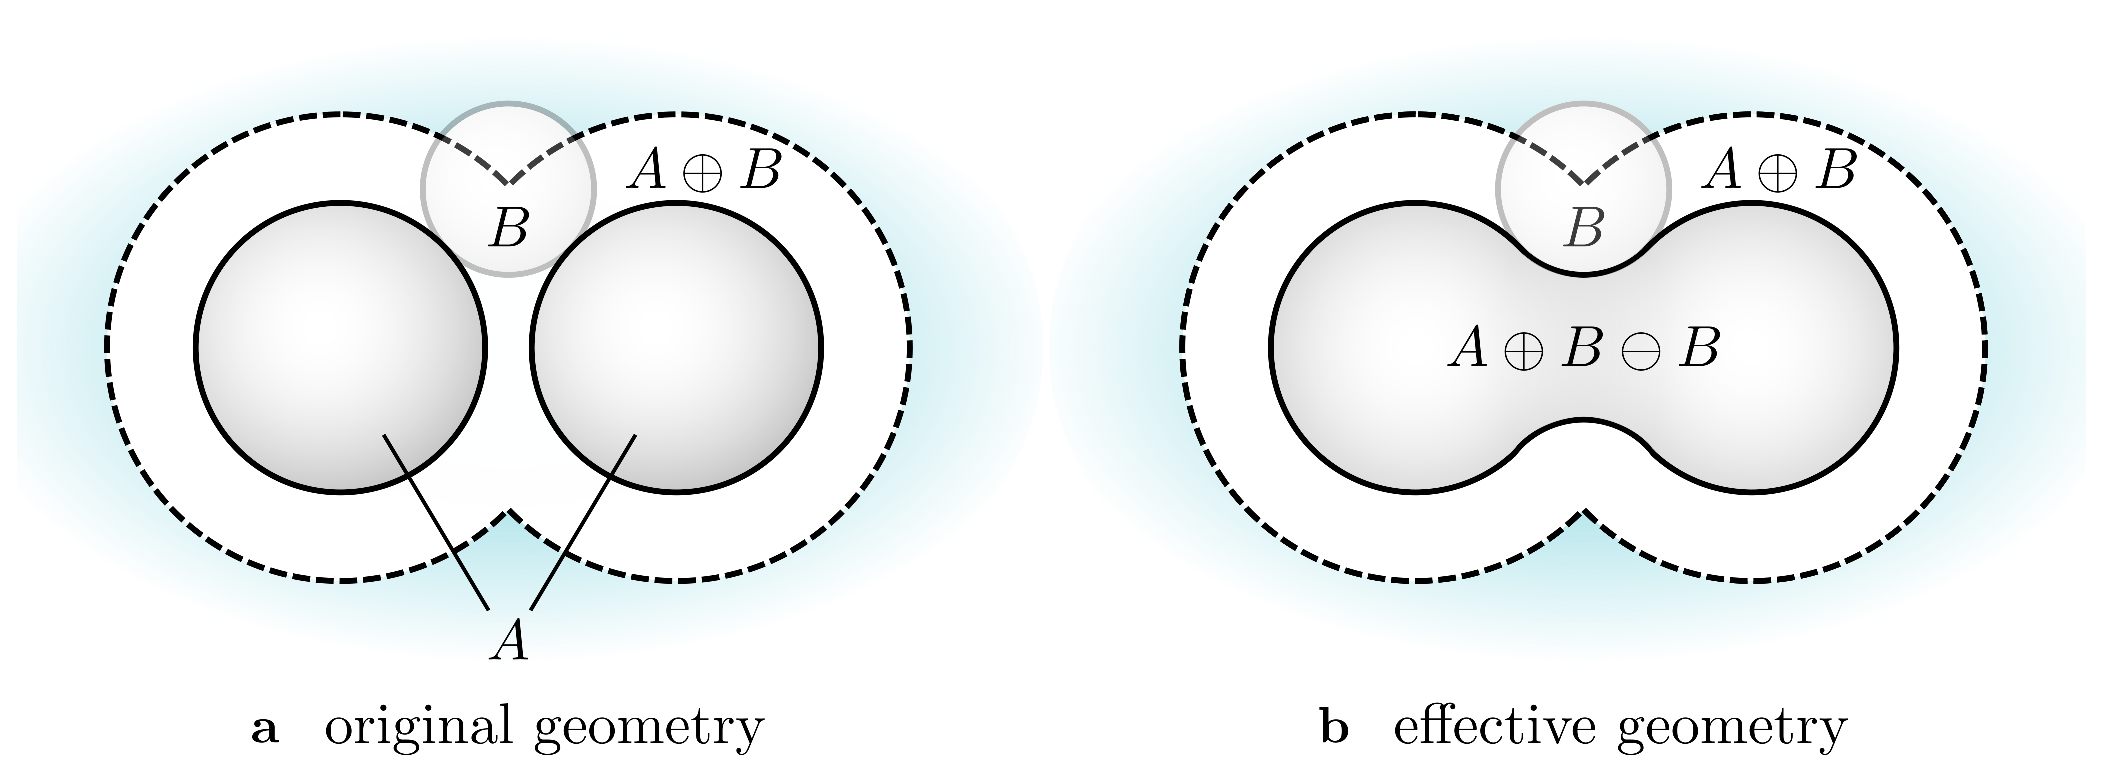
\includegraphics[width=0.9\linewidth,center]{minkowski-addition}
%%   \caption[Minkowski addition and difference]{
%%     Minkowski addition and difference.
%%     Note how these are not inverse operations.}
%% \end{SCfigure}

%% \vspace{0.5em}
%% \begin{tcolorbox}[title=Steiner's formula for parallel volumes]
%%   For a compact, convex body $K \in \mathcal{K}^d$ the parallel volume is expressable as:
%%   \begin{equation}
%%     V_d[K + \epsilon \ball_d] =
%%     \sum_{i=0}^d V_i[K] \omega_{d-i} \epsilon^{d-i}
%%   \end{equation}
%% \end{tcolorbox}

\subsection{Kinematic formulas}
\label{sec:kinematic-formula}

Here we introduce the \emph{kinematic formulas} which calculate hitting probabilities, i.e.\ the probability that randomly distributed objects collide.
This problem is applicable to the evaluation of partition functions in statistical mechanics, of which we will see specific examples in section \ref{sec:fmt} and chapter \ref{chapter:resummation}.

Two compact and convex objects $K_1, K_2 \in \mathcal{K}^d$ overlap if their intersection is non-empty $K_1 \cap K_2 \ne \emptyset$.
The intersection of convex objects is also convex, so from the definition of the Euler characteristic \eqref{eq:euler-characteristic-definition} we can write
\begin{equation*}
  \chi[K_1 \cap K_2]
  =
  \begin{cases}
    1 & \textrm{ if } K_1 \cap K_2 \ne \emptyset \\
    0 & \textrm{ if } K_1 \cap K_2 = \emptyset
  \end{cases}
\end{equation*}
then the probability that the two objects collide is
\begin{equation*}
  \mathrm{Prob} \left[ \textrm{collision} \right]
  =
  \frac{1}{V} \int_V \chi[K_1 \cap K_2(\vec{r})] \, d\vec{r}
\end{equation*}
where $K_2$ is uniformly distributed and $K_1$ acts as a fixed target.
Here, $K_2$ is \emph{translated} over the accessible volume, however in general these objects will be non-spherical so we should also consider the \emph{rotations}.
Integral geometry more naturally deals with integrations over relative positions \emph{and} orientations, at the small cost of additional notation.
%In addition to integrations over particle positions $\{\vec{r}_1, \cdots, \vec{r}_n\}$ we also have to consider their orientations $\{\vec{\theta}_1, \cdots, \vec{\theta}_n\}$ where each $\vec{\theta}_i$ represents an Euler angle tuple.
%Then, assuming an isotropic phase where all orientations are equally likely each positional integral generalises to
Writing the relative orientation as the Euler angle tuple $\vec{\theta}$, we consider the generalisation
\begin{equation*}
  \int_{\mathbb{R}^d} d\vec{r}
  \to
  \int_{\mathbb{R}^d \times SO(d)} d\vec{r} d\vec{\theta}
  :=
  \int_{G_d} dg,
\end{equation*}
with the normalisation in the angular measure such that $\int d\vec{\theta} = 1$.
In the right-most equality we introduced the rigid-motion operation acting on a body $K \in \mathcal{K}^d$ as
\begin{equation*}
  g K := \{\mathcal{R}_\theta \, \vec{k} + \vec{r} \, | \, \vec{k} \in K\},
  %(\mathcal{T} \circ \mathcal{R})(\vec{r}, \vec{\theta}),
\end{equation*}
a member of the rigid motion group $g \in G_d := \mathbb{R}^d \times \mathrm{SO}(d)$, and where $\mathcal{R}_\theta \in \mathrm{SO}(d)$%
\marginfootnote{$\mathrm{SO}(d)$ is the \emph{special orthogonal group}, i.e.\ the group of all orthogonal matrices with unit determinant.}
is the rotation matrix parameterised by $\vec{\theta}$.
Then the generalised measure for particle collisions becomes
\begin{equation*}
  \int_{G_d} \chi[K_1 \cap g K_2] \, dg
\end{equation*}
if they occupy all of Euclidean space.
We will see integrals like this emerge from liquid state theory in sections \ref{sec:virial-series} and \ref{sec:fmt}, and later in chapter \ref{chapter:resummation}.

\vspace{0.5em}
\begin{tcolorbox}[title=Principal kinematic formula]
  %% Noting that $\chi = V_0$ is the lowest order intrinsic volume, the latter line of \eqref{eq:low-density-insertion} is ideally suited to a treatment within integral geometry.
  A central result of integral geometry is the principal kinematic formula of Blaschke and Santal\'o \cite{BlaschkeMZ1936,Blaschke1937,SantaloASI1936} which gives the explicit form of these collisional integrals as \cite{Santalo2004,Klain1997}
  %\cite{Santalo2004,SchneiderACIG1984,Schneider2008,Klain1997}
  \begin{equation}\label{eq:binomial-kinematic-formula}
    \int_{G_d} \chi[K_1 \cap g K_2] \, dg
    =
    \sum_{k=0}^d (C_{k,d-k})^{-1} V_k[K_1] V_{d-k}[K_2]
  \end{equation}
  We see the flag coefficients \eqref{eq:flag-coefficients} play an analogous role here in conjugating the intrinsic volumes as binomial coefficients do in algebraic expansions%
  \marginfootnote{For this reason Klain and Rota argue that integral geometry should be called \emph{continuous combinatorics} \cite{Klain1997}, because it generalises combinatorial results to continuous spaces}.
  More general formulas exist for more general integrals over $V_k[K_1 \cap K_2]$ for all $k$ \cite{Klain1997}, however these do not have an interpretation in terms of evaluating partition functions so we will not be using them.
\end{tcolorbox}

The principal kinematic formula \eqref{eq:binomial-kinematic-formula} can be iterated for the intersections of many bodies $\{K_1, \cdots, K_n\}$ giving \cite{Santalo2004,MarechalPRE2014}
\begin{subequations}\label{eq:multinomial-kinematic-formula}
  \begin{equation}
    \begin{split}
      & \quad
      \int_{G_d^n} \chi[K_1 \cap g_2 K_2 \cap \cdots \cap g_n K_n]
      \, dg_2 \cdots dg_n
      \\ = &
      \sum_{\substack{i_1, \cdots, i_n = 0 \\ i_1 + \cdots + i_n = nd}}^d
      (C_{i_1, \cdots, i_n})^{-1}
      V_{i_1}(K_1)
      \prod_{j=2}^n
      V_{i_j}(K_j)
    \end{split}
  \end{equation}
  \begin{equation}
    \textrm{with} \qquad
    C_{i_1, \cdots, i_n}
    := \frac{1}{i_1! \omega_{i_1}}
    \prod_{j=2}^n
    \left(
    \frac{d!}{i_j!} \frac{\omega_d}{\omega_{i_j}}
    \right)
  \end{equation}
\end{subequations}
where $C_{i_1, \cdots, i_n}$ would be the multinomial generalisation of the flag coefficients \eqref{eq:flag-coefficients}.
We will use this iterated formula in chapter \ref{chapter:resummation} to resum a piece of the virial series (to be introduced in the upcoming section \ref{sec:virial-series}).

%% We have the invariant measure on 1-dimensional linear subspaces of $\mathbb{R}^d$ (\emph{Grassmanians}) as
%% \begin{equation}
%%   [d] = \tau_d(\textrm{Gr}(d,1))
%%   = \frac{d \omega_d}{2 \omega_{d-1}}.
%% \end{equation}
%% Factorial defined as
%% \begin{equation}
%%   [k]! = \prod_{i=0}^k \, [i]
%% \end{equation}
%% Flag coefficients from binomial coefficients
%% \begin{equation}
%%   {d \brack k}
%%   := \frac{[n]!}{[k]! [n-k]!}
%%   = {d \choose k}
%%   \frac{\omega_d}{\omega_k \omega_{d-k}}
%% \end{equation}
%% Provides the generalisation of combinatorial results to continuous spaces.
%% Analagously to binomial coefficients, the flag coefficients obey
%% \begin{equation}\label{eq:flag-coefficients-symmetry}
%%   {d \brack k} = {d \brack d - k}.
%% \end{equation}
%% Note that we can rewrite \eqref{eq:intrinsic-volume-ball} using the flag coefficients as
%% \begin{equation}\label{eq:intrinsic-volume-ball-flag}
%%   \mu_k (\ball_d) = {d \choose k} \frac{\omega_d}{\omega_{d-k}}
%%   = {d \brack k} \omega_k
%% \end{equation}

%% \begin{center}
%% \begin{tabular}{cccccc}
%%   \toprule
%%   $k$ & $\omega_k$ & $[k]$ & $[k]!$ & ${2 \brack k}$ & ${3 \brack k}$ \\
%%   \midrule
%%   0 & 1 & 1 & 1 & 1 & 1 \\
%%   1 & 2 & 1 & 1 & $\frac{\pi}{2}$ & 2 \\
%%   2 & $\pi$ & $\frac{\pi}{2}$ & $\frac{\pi}{2}$ & 1 & 2 \\
%%   3 & $\frac{4\pi}{3}$ & 2 & $\pi$ & & 1 \\
%%   \bottomrule
%% \end{tabular}
%% \end{center}

%% \vspace{0.5em}
%% \begin{tcolorbox}[title=General kinematic formula]
%%   For $0 \le k \le d$:
%%   \begin{equation}
%%     \int_{\mathbb{E}_d} \mu_k (A \cap g B) \, dg =
%%     \sum_{i=0}^{d-k}
%%     {i + k \brack k} {d \brack i}^{-1}
%%     \mu_{i+k}(A) \mu_{d-i}(B)
%%   \end{equation}
%%   \begin{equation*}
%%     \int_{\mathbb{E}_d} \mu_k (A \cap g B) \, dg =
%%     \sum_{i=0}^{d-k}
%%     {i + k \brack k}
%%     {d \brack i + k}
%%     \kappa_{i+k}(A) \kappa_{d-i}(B)
%%   \end{equation*}
%%   In regular binomial:
%%   \begin{equation*}
%%     \int_{\mathbb{E}_d} \mu_k (A \cap g B) \, dg =
%%     \sum_{i=0}^{d-k}
%%     {i + k \choose k} {d \choose i}^{-1}
%%     \frac{\omega_{i+k} \omega_{d-i}}{\omega_k \omega_d}
%%     \mu_{i+k}(A) \mu_{d-i}(B)
%%   \end{equation*}
%% \end{tcolorbox}

%% \begin{equation*}
%%   {n \choose k} {k \choose p}
%%   =
%%   \frac{n!}{k!(n-k)!}
%%   \frac{k!}{p!(k-p)!}
%%   =
%%   \frac{n!}{p!(k-p)!(n-k)!}
%%   =
%%   {n \choose p, k-p, n-k}
%% \end{equation*}
%% I.e. this is a trinomial coefficient.
%% So we have
%% \begin{equation*}
%%   {n \brack k} {k \brack p}
%%   =
%%   {n \choose k}
%%   {k \choose p}
%%   \frac{\omega_n}{\omega_k \omega_{n-k}}
%%   \frac{\omega_k}{\omega_p \omega_{k-p}}
%%   =
%%   {n \choose p, k-p, n-k}
%%   \frac{\omega_n}{\omega_p \omega_{k-p} \omega_{n-k}}
%% \end{equation*}

\section{Statistical physics of fluids}
\label{sec:liquid-state-theory}

%% \subsection{Notes}

%% Here we talk in general terms about descriptions of the liquid state.
%% Broadly speaking, in its historical development approaches can be placed inside one of two categories.
%% Namely, theories involving
%% \begin{enumerate}
%%   \item Local geometric approximations capturing the short range interactions (free volume theory/cell theory, scaled particle theory), and
%%   \item Integral equations (Ornstein-Zernike closures, density functional theory) which properly treat the long range correlations.
%% \end{enumerate}
%% These two approaches are not mutually exclusive, and hybrid theories can improve on.
%% For instance, fundamental measure theory (FMT) involves the synthesis of integral geometry with the formalism of density functional theory which involves minimising a functional (i.e.\ an integral equation).

%% Classical theory of phase transitions (Landau).
%% Van der waals theory.
%% How does the transition occur?
%% Metastability leads into kinetics.

%% Kinetics vs thermodynamics.
%% Thermodynamic driving force vs activation barrier.

%% Relaxation behaviour controlled by activation barrier.
%% A thermal fluctuation which takes the system over the barrier%
%% \marginfootnote{These fluctuations are conventionally called \emph{instantons} as they spontaneously appear and vanish just like virtual particles in fundamental physics.
%%   The name for this relatively straightforward phenomenon is thus a reference to a much more counterintuitive and bizarre phenomenon, because physicists are good at making helpful analogies.}
%% occurs with rate $\exp{-\beta \Delta U}$ \cite{Langer}.

%% Liquids:
%% Free volume theory.
%% Early curvature corrections.
%% Free volume theory depends on the free volume (duh).
%% This is an example of an integral geometric theory.
%% Morphological

\subsection{Statistical mechanics}
\label{sec:stat-mech}

In this section we \emph{briefly} introduce the statistical ensembles used throughout the rest of the thesis.
These emerge by considering typical fluctuations of thermodynamic quantities for a subsystem within a macroscopic system called the \emph{ensemble}; the properties of this larger system define average quanties of the subsystem \cite{Landau2008}.
Alternatively, the same formalism can be interpretted from a Bayesian perspective to emerge from maximisation of the entropy%
\marginfootnote{The entropy represents a thermodynamic quantity in the former picture, whereas it represents our own \emph{uncertainty} about the system in the latter.}
subject to the constraint of average energy and (optionally) the average particle number \cite{JaynesPR1957,JaynesPR1957a}.

A $d$-dimensional system of $N$ particles consists of $\vec{r}^N = \{\vec{r}_1, \cdots, \vec{r}_N\} \in \mathbb{R}^{dN}$ coordinates and $\vec{p}^N = \{\vec{p}_1, \cdots, \vec{p}_N\} \in \mathbb{R}^{dN}$ momenta.
The classical Hamiltonian can be decomposed into kinetic and potential terms as in
\begin{equation}
  \mathcal{H}_N(\vec{r}^N, \vec{p}^N)
  =
  K_N(\vec{p}^N) + U_N(\vec{r}^N)
\end{equation}
in the absence of an external field.
Further, we constrain the coordinates inside the volume $V$.
The \emph{canonical} ensemble describes an equilibrium system at constant temperature $T$ with probability measure%
\marginfootnote{As a reminder for the reader, in the previous chapter we introduced $\beta = (k_B T)^{-1}$, with Boltzmann constant $k_B$ and temperature $T$.}[2cm]
\begin{equation}
  f^{(N)}(\vec{r}^N, \vec{p}^N) \propto e^{-\beta \mathcal{H}_N}.
\end{equation}
The proportionality constant ensures the probability distribution is properly normalised, leading to the canonical partition function
\begin{equation}
  Q_N
  =
  \int_{\mathbb{R}^{dN}} \int_{V^N}
  e^{-\beta\mathcal{H}_N}
  d\vec{r}^N d\vec{p}^N.
\end{equation}
Classically, the kinetic energy is simply
\begin{equation*}
  K_N(\vec{p}^N) = \sum_{i=1}^N \frac{|\vec{p}_i|^2}{2m_i}
\end{equation*}
which can be integrated leaving
\begin{equation}
  Q_N = \frac{Z_N}{\Lambda^{dN} N!}
\end{equation}
where $\Lambda$ is the thermal de Broglie wavelength, and the configurational integral is given by
\begin{equation}\label{eq:canonical-partition}
  Z_N
  =
  \int_{V^N}
  e^{-\beta U_N}
  d\vec{r}^N.
\end{equation}
Averaged quantities with $N$ fixed are obtained through
\begin{equation*}\label{eq:canonical-average}
  \left< \cdots \right>_N
  =
  \frac{1}{Z_N}
  \int_{V^N} \left(\cdots\right) e^{-\beta U_N} d\vec{r}^N,
\end{equation*}
and the Helmholtz free energy is given by
\begin{equation*}
  \beta F = -\ln{Z_N}.
\end{equation*}

We will work almost exclusively in the \emph{grand canonical ensemble}, where particle number varies according to a chemical potential $\mu$, which is convenient for liquid state descriptions%
\marginfootnote{Notably the free energy is extensive without invoking Stirling's approximation for $N!$, making the thermodynamics properly self-consistent even with small system sizes.}.
The corresponding partition function features summation over $N$, as in
\begin{equation}\label{eq:grand-canonical-partition}
  \Xi
  =
  \sum_{N=0}^\infty \frac{z^N}{N!} Z_N
  =
  \sum_{N=0}^\infty \frac{z^N}{N!}
  \int_{V^N} e^{-\beta U_N} d\vec{r}^N,
\end{equation}
where the activity is $z = \exp{(\beta\mu)} / \Lambda^d$.
Accordingly, average quantities are found via
\begin{equation}\label{eq:grand-canonical-average}
  \left< \cdots \right>
  =
  \frac{1}{\Xi} \sum_{N=0}^\infty \frac{z^N}{N!}
  \int_{V^N} \left(\cdots\right) e^{-\beta U_N} d\vec{r}^N,
\end{equation}
and the corresponding free energy (or \emph{grand potential}) is obtained via
\begin{equation*}
  \beta \Omega = -\ln{\Xi}.
\end{equation*}
For a homogeneous system this reduces to the standard result
\begin{equation}\label{eq:homogeneous-grand-potential}
  \Omega_\mathrm{hom} = - p V.
\end{equation}
Thermodynamic quantities are easily calculated for the ideal gas, e.g.\
\begin{equation*}
  \beta\Omega = - \frac{e^{\beta\mu^\mathrm{id}}}{\Lambda^d} V.
\end{equation*}
Comparing the homogeneous result \eqref{eq:homogeneous-grand-potential} with the ideal gas law $\beta p = \rho$ gives the chemical potential of an ideal gas as
\begin{equation}\label{eq:ideal-chemical-potential}
  \beta \mu^\mathrm{id} = \ln{(\Lambda^d \rho)}.
\end{equation}
From the Legendre transform of the grand potential
\begin{equation}\label{eq:grand-potential-legendre-transform}
  \Omega = F - \mu N
\end{equation}
we obtain the free energy density of an ideal gas as
\begin{equation}\label{eq:ideal-free-energy-density}
  \frac{\beta F^\mathrm{id}}{V} = \rho (\ln{(\Lambda^d \rho)} - 1).
\end{equation}
Finally, for interacting systems the chemical potential and free energy are typically separated into \emph{ideal} and \emph{excess} parts, as in
\begin{align*}
  \beta \mu &= \beta \mu^\mathrm{id} + \beta \mu^\mathrm{ex},
  \\
  \beta F &= \beta F^\mathrm{id} + \beta F^\mathrm{ex},
\end{align*}
with the ideal contributions as expressed above.

\subsection{Liquid structure}
\label{sec:liquid-structure}

Interparticle interactions induce spatial structure in the liquid which are characterised by several (equivalent) hierarchies of correlation functions.
The most natural description of structure starts from the \emph{$n$-particle density}
\begin{equation}\label{eq:n-particle-density-pdf}
  \mathrm{Prob}\left[ \textit{any } n \textrm{ particles in volume } d\vec{r}^n \right]
  :=
  \rho^{(n)}(\vec{r}^n) \, d\vec{r}^n,
\end{equation}
where $\vec{r}^n := \{\vec{r}_1, \cdots, \vec{r}_n\}$ are the particle positions.
This is formally obtained by integrating the full (configurational) probability distribution over the remaining degrees of freedom.
For the single-component system this yields \cite{Hansen2013}
\begin{equation}\label{eq:n-particle-density}
  \rho^{(n)}(\vec{r}^n)
  =
  \frac{1}{\Xi}
  \sum_{N=n}^\infty \frac{z^N}{(N-n)!}
  \int_{V^N} e^{-\beta U_N} \, d\vec{r}^{(N-n)}.
\end{equation}
The $n$-particle density is an intuitive descriptor for liquid structure because it generalises the probability density function for a closed system, i.e.\
\begin{equation*}
  \mathrm{Prob}\left[ N \textrm{ particles in volume } d\vec{r}^n \right]
  :=
  \frac{e^{-\beta U_N}}{Z_N} \, d\vec{r}^N,
\end{equation*}
to a subset of particles within an open system.
$\rho^{(n)}$ thus provides the correct procedure for coarse-graining onto selected degrees of freedom within a bulk system.
The analogy with the canonical ensemble is imperfect in that $\rho^{(n)}$ is unnormalised so it is not strictly a probability density function; integrating \eqref{eq:n-particle-density} over the remaining degrees of freedom yields%
\marginfootnote{In keeping with the analogy to canonical ensemble we treat this integral as a partition function, and so account for indistinguishability of the $n$ particles by dividing through by $n!$.}
\begin{equation*}\label{eq:n-particle-density-normalisation}
  \frac{1}{n!}
  \int_{V^n} \rho^{(n)}(\vec{r}^n) \, d\vec{r}^n
  =
  \left\langle \frac{N!}{n! (N-n)!} \right\rangle
\end{equation*}
i.e.\ the average binomial coefficient.
The $n$-particle density scales proportionally to $\rho^n$ so it is usual to remove this by defining the \emph{$n$-particle distribution function} as
\begin{equation}\label{eq:n-particle-distribution}
  g^{(n)}(\vec{r}^n)
  :=
  \frac{\rho^{(n)}(\vec{r}^n)}{\prod_{i=1}^n \rho^{(1)}(\vec{r}_i)},
\end{equation}
which provides our first (and primary) hierarchy of correlation functions.

Physically, particles become decorrelated when they are separated by macroscopic distances%
\marginfootnote{This limit behaviour is only valid for `normal' liquid behaviour far from the critical point where the correlation length diverges.}.
This property manifests in the distribution functions via a \emph{product property} where \cite{UhlenbeckJMP1963}
\begin{equation*}
  g^{(n)}(\vec{r}^n)
  \simeq
  g^{(s)}(\vec{r}^s) \, g^{(n-s)}(\vec{r}^{n-s})
\end{equation*}
in the limit where the $s$ particles become macroscopically separated from the remaining $(n-s)$ particles.
This property causes the distribution functions to decay to their ideal gas value $g^{(n)}(\vec{r}^n) \to 1$ in the limit of infinite separations between all particles.
Moreover, the product property suggests that there is a great deal of redundancy inside the distribution functions; in certain applications it is convenient to introduce an additional hierarchy of correlation functions which only capture the excess correlations.
If we imagine the normalisation of the distribution functions $g^{(n)}$ as \emph{moments} of an unspecified probability distribution, then we can formally imagine a dual set of correlation functions $h^{(n)}$ which generate the \emph{cumulants}.
Formally, this relationship is expressed \cite{Santos2016}
\begin{equation*}\label{eq:correlation-moment-generating-function}
  1
  + \sum_{n=1}^\infty \frac{\epsilon^n}{n!}
  \int_{V^n} g^{(n)}(\vec{r}^n) \, d\vec{r}^n
  =
  \exp{
    \left(
    \sum_{n=1}^\infty \frac{\epsilon^n}{n!}
    \int_{V^n} h^{(n)}(\vec{r}^n) \, d\vec{r}^n
    \right)
  },
\end{equation*}
with $\epsilon$ as a formal expansion parameter of the moment generating function.
In addition, we require that these new functions share the same symmetries as $g^{(n)}$ e.g.\ permutation invariance in the arguments.
These conditions specify a new hierarchy: the \emph{cluster correlation functions}%
\marginfootnote{These are so-named because they possess a \emph{cluster property} where they decay to zero in the limit where any particles become macroscopically separated \cite{UhlenbeckJMP1963}.
  This feature directly emerges from, and is dual to, the product property for $g^{(n)}$.}
where the first few terms are given by \cite{UhlenbeckJMP1963}
\begin{subequations}\label{eq:cluster-correlation-functions}
  \begin{align}
    h^{(1)}(\vec{r})
    =& \,
    g^{(1)}(\vec{r}),
    \\
    h^{(2)}(\vec{r}_1, \vec{r}_2)
    =& \,
    g^{(2)}(\vec{r}_1, \vec{r}_2)
    - g^{(1)}(\vec{r}_1) g^{(1)}(\vec{r}_2),
    \label{eq:pair-cluster-correlation-function}
    \\
    h^{(3)}(\vec{r}_1, \vec{r}_2, \vec{r}_3)
    =& \,
    g^{(3)}(\vec{r}_1, \vec{r}_2, \vec{r}_3)
    - \{3\} g^{(2)}(\vec{r}_1, \vec{r}_2) g^{(1)}(\vec{r}_3)
    %- g^{(2)}(\vec{r}_2, \vec{r}_3) g^{(1)}(\vec{r}_1)
    \nonumber \\ & \,
    %- g^{(2)}(\vec{r}_3, \vec{r}_1) g^{(1)}(\vec{r}_2)
    + g^{(1)}(\vec{r}_1) g^{(1)}(\vec{r}_2) g^{(1)}(\vec{r}_3),
  \end{align}
\end{subequations}
where $\{\cdot\}$ indicates the number of similar terms which differ only by permutation of indices which we omit for brevity.
The pair cluster correlation function%
\marginfootnote{This is often called simply the \emph{total correlation function}, especially in the context of integral equation theories (cf.\ section \ref{sec:oz-equation}).}
$h^{(2)}(\vec{r}_1, \vec{r}_2) = g^{(2)}(\vec{r}_1, \vec{r}_2) - 1$ is the main function we will use from this hierarchy.

We can define two further hierarchies of correlation functions from the moments and fluctuations in the density.
Writing the instantaneous density as
\begin{equation*}\label{eq:instantaneous-density}
  \hat\rho(\vec{r}) = \sum_{i=1}^N \delta(\vec{r} - \vec{r}_i)
\end{equation*}
where $\delta(\cdot)$ is the Dirac delta function, then the various \emph{density moments} are determined as
%% Similarly, we can define higher-order moments of the instantaneous density in terms of $\rho^{(n)}$ giving e.g.\
\begin{subequations}\label{eq:density-moments}
  \begin{align}
    \langle \hat\rho(\vec{r}) \rangle
    =& \,
    \rho^{(1)}(\vec{r}),
    \label{eq:single-particle-density}
    \\
    \big\langle \hat\rho(\vec{r}_1) \hat\rho(\vec{r}_2) \big\rangle
    =& \,
    \rho^{(2)}(\vec{r}_1, \vec{r}_2) +
    \rho^{(1)}(\vec{r}_1) \delta(\vec{r}_1 - \vec{r}_2),
    \\
    \big\langle \hat\rho(\vec{r}_1) \hat\rho(\vec{r}_2) \hat\rho(\vec{r}_3) \big\rangle
    =& \,
    \rho^{(3)}(\vec{r}_1, \vec{r}_2, \vec{r}_3) +
    \{3\} \rho^{(2)}(\vec{r}_1, \vec{r}_2) \delta(\vec{r}_1 - \vec{r}_3)
    \nonumber \\ & \,
    + \rho^{(1)}(\vec{r}_1) \delta(\vec{r}_1 - \vec{r}_2) \delta(\vec{r}_1 - \vec{r}_3).
  \end{align}
\end{subequations}
Importantly, \eqref{eq:single-particle-density} shows that the single-particle density is simply the equilibrium density profile.
The normalisation of these functions gives the moments of particle number $N$, i.e.\
\begin{equation}
  \int_{V^n}
  \left\langle
  \prod_{i=1}^n \hat\rho(\vec{r}_i)
  \right\rangle
  \, d\vec{r}^n
  =
  \left\langle N^n \right\rangle.
\end{equation}
We can define a dual hierarchy of \emph{density-density correlation functions} $H^{(n)}$ by the same procedure used to generate $h^{(n)}$ from $g^{(n)}$, i.e.\ through a cumulant generating function.
The first few functions in this hierarchy are
\begin{subequations}\label{eq:density-density-correlations}
  \begin{align}
    H^{(1)}(\vec{r})
    =& \,
    %% \big\langle \hat\rho(\vec{r}) \big\rangle
    %% =
    \rho^{(1)}(\vec{r}),
    \\
    H^{(2)}(\vec{r}_1, \vec{r}_2)
    =& \,
    \big\langle \hat\rho(\vec{r}_1) \hat\rho(\vec{r}_2) \big\rangle
    - \rho^{(1)}(\vec{r}_1) \rho^{(1)}(\vec{r}_2),
    \label{eq:pair-density-density-correlation}
    \\
    H^{(3)}(\vec{r}_1, \vec{r}_2, \vec{r}_3)
    =& \,
    \big\langle \hat\rho(\vec{r}_1) \hat\rho(\vec{r}_2) \hat\rho(\vec{r}_3) \big\rangle
    - \{3\} \big\langle \hat\rho(\vec{r}_1) \hat\rho(\vec{r}_2) \big\rangle \rho^{(1)}(\vec{r}_3)
    %- \big\langle \hat\rho(\vec{r}_2) \hat\rho(\vec{r}_3) \big\rangle \rho^{(1)}(\vec{r}_1)
    \nonumber \\ & \,
    %- \big\langle \hat\rho(\vec{r}_3) \hat\rho(\vec{r}_1) \big\rangle \rho^{(1)}(\vec{r}_2)
    + \rho^{(1)}(\vec{r}_1) \rho^{(1)}(\vec{r}_2) \rho^{(1)}(\vec{r}_3),
  \end{align}
\end{subequations}
or more generally \cite{Hansen2013}
\begin{equation}\label{eq:density-density-correlations}
  H^{(n)}(\vec{r}^n)
  =
  \left\langle
  \prod_{i=1}^n
  \Big[ \rho(\vec{r}_i) - \rho^{(1)}(\vec{r}_i) \Big]
  \right\rangle
  \qquad \forall \; n \ge 2.
\end{equation}
The normalisations of $H^{(n)}$ give the cumulants in $N$ i.e.\
\begin{equation*}
  \int_{V^n} H^{(n)}(\vec{r}^n) \, d\vec{r}^n
  =
  \frac{d^n}{d\epsilon^n}
  \left[
  \log{\left(
      1 + \sum_{m=1}^\infty
      \frac{\epsilon^m}{m!} \left\langle N^m \right\rangle
      \right)}
  \right]_{\epsilon = 0}
\end{equation*}
or explicitly for the first few functions
\begin{subequations}
  \begin{align}
    \int_V H^{(1)}(\vec{r}) \, d\vec{r}
    &=
    \langle N \rangle,
    \\
    \int_{V^2} H^{(2)}(\vec{r}_1, \vec{r}_2) \, d\vec{r}_1 d\vec{r}_2
    &=
    \langle N^2 \rangle - \langle N \rangle^2,
    \label{eq:pair-density-density-norm}
    \\
    \int_{V^3} H^{(3)}(\vec{r}_1, \vec{r}_2, \vec{r}_3) \, d\vec{r}_1 d\vec{r}_2 d\vec{r}_3
    &=
    \langle N^3 \rangle
    - 3 \langle N^2 \rangle \langle N \rangle
    + 2 \langle N \rangle^3.
  \end{align}
\end{subequations}
This class of correlation functions thus describes the fluctuations in density, which can play an important thermodynamic role; we will give a specific example of how these functions connect to thermodynamic response functions below.

An important response function for liquid structure is the isothermal compressibility
\begin{equation*}\label{eq:isothermal-compressibility}
  \kappa_T
  :=
  %% - \frac{1}{V}
  %% \left( \frac{\partial V}{\partial p} \right)_{N,T}.
  \frac{1}{\rho}
  \left( \frac{\partial \rho}{\partial p} \right)_{V,T}.
\end{equation*}
Using standard thermodynamic manipulations we can obtain the equivalent expression
\begin{equation*}
  \kappa_T
  =
  \frac{1}{\rho^2}
  \left( \frac{\partial \rho}{\partial \mu} \right)_{V,T}
\end{equation*}
or defining the dimensionless \emph{isothermal susceptibility} as \begin{equation*}\label{eq:isothermal-susceptibility}
  \chi_T
  :=
  \rho k_B T \kappa_T
  =
  \frac{1}{\rho}
  \left( \frac{\partial \rho}{\partial (\beta \mu)} \right)_{V,T}.
\end{equation*}
It is straightforward to evaluate this through the grand canonical average \eqref{eq:grand-canonical-average} of density $\rho = \langle N \rangle / V$, obtaining
\begin{equation}
  \chi_T
  =
  \frac{ \langle N^2 \rangle - \langle N \rangle^2 }{\langle N \rangle}.
\end{equation}
From the normalisation of $H^{(2)}$ \eqref{eq:pair-density-density-norm} as the second cumulant in $N$, we find
\begin{equation}\label{eq:compressibility-h2}
  \begin{split}
    \chi_T
    &=
    \frac{1}{\langle N \rangle}
    \int_{V^2} H^{(2)}(\vec{r}_1, \vec{r}_2) \, d\vec{r}_1 d\vec{r}_2
    \\ &=
    1
    + \rho \int_V h^{(2)}(\vec{r}) \, d\vec{r}
  \end{split}
\end{equation}
where the latter step is valid for the homogeneous liquid where $g^{(2)}(\vec{r}_1, \vec{r}_2) = g^{(2)}(\vec{r}_2 - \vec{r}_1)$ and we used the pair cluster correlation function \eqref{eq:pair-cluster-correlation-function}.

The various correlation functions introduced are all structural descriptors in real space, but we can imagine equivalent descriptors in Fourier space.
The most important Fourier space correlation are the static structure factors $S^{(n)}$, of which the pair structure factor $S^{(2)}$ is particularly important for scattering experiments.
We define this from the Fourier transform of the pair distribution function in the case of the uniform liquid as
\begin{equation}\label{eq:static-structure-factor}
  \begin{split}
    S^{(2)}(\vec{k})
    :=&
    \frac{
      \big\langle \tilde{\rho}(\vec{k}) \tilde{\rho}(-\vec{k}) \big\rangle
    }{
      \langle N \rangle
    }
    =
    1 + \rho \tilde{g}^{(2)}(\vec{k})
    \\ =&
    1 + \rho \tilde{h}^{(2)}(\vec{k}) + \rho \delta(\vec{k})
  \end{split}
\end{equation}
where the tilde over a function denotes its Fourier transform.
In terms of the structure factor \eqref{eq:compressibility-h2} is written succinctly as%
\marginfootnote{The Dirac delta function at the origin in $S^{(2)}(\vec{k})$ is often omitted to regularise the function, in which case the right-hand side can be written more simply as $S^{(2)}(0)$.}
\begin{equation}
  \chi_T = \lim_{\vec{k} \to 0} S^{(2)}(\vec{k}).
\end{equation}

%% \todo{Kirkwood superposition and convolution approximations}

%% \subsection{?}

%% \todo{Finish this section}

%% \begin{equation}
%%   \chi_T \rho
%%   \left( \frac{\partial \rho^{(n)}}{\partial \rho} \right)_{V,T}
%%   =
%%   (n - \rho V) \rho^{(n)}(\vec{r}^n)
%%   + \int \rho^{(n+1)}(\vec{r}^{n+1}) \, d\vec{r}_{n+1}
%% \end{equation}
%% \begin{equation}
%%   \left( \frac{\partial g^{(n)}(\vec{r}^n)}{\partial \rho} \right)_{V,T}
%%   =
%%   \frac{1}{\rho^n}
%%   \left( \frac{\partial \rho^{(n)}(\vec{r}^n)}{\partial \rho} \right)_{V,T}
%%   - \frac{n}{\rho} g^{(n)}(\vec{r}^n)
%% \end{equation}
%% \begin{equation}
%%   \begin{split}
%%     \frac{\chi_T}{\rho^n}
%%     \left( \frac{\partial \rho^{(n)}}{\partial \rho} \right)_{V,T}
%%     &=
%%     \left(\frac{n}{\rho} - V\right) g^{(n)}(\vec{r}^n)
%%     + \int g^{(n+1)}(\vec{r}^{n+1}) \, d\vec{r}_{n+1}
%%     \\ &=
%%     \chi_T \left( \frac{\partial g^{(n)}}{\partial \rho} \right)_{V,T}
%%     + \chi_T \frac{n}{\rho} g^{(n)}
%%   \end{split}
%% \end{equation}
%% \begin{equation}
%%   \chi_T \left( \frac{\partial g^{(n)}}{\partial \rho} \right)_{V,T}
%%   =
%%   \left(
%%   \frac{n (1 - \chi_T)}{\rho}
%%   - V
%%   \right) g^{(n)}(\vec{r}^n)
%%   + \int g^{(n+1)}(\vec{r}^{n+1}) \, d\vec{r}_{n+1}
%% \end{equation}
%% \begin{equation}
%%   \begin{split}
%%     \chi_T \left( \frac{\partial g^{(2)}}{\partial \rho} \right)_{V,T}
%%     &=
%%     \left(
%%     \frac{2 (1 - \chi_T)}{\rho}
%%     - V
%%     \right) g^{(2)}(\vec{r}^2)
%%     + \int g^{(3)}(\vec{r}^3) \, d\vec{r}_3
%%     \\
%%     \left( \frac{\partial g^{(2)}}{\partial \rho} \right)_{V,T}
%%     &=
%%     \frac{2 (1 - \chi_T)}{\rho \chi_T}
%%     g^{(2)}(\vec{r}^2)
%%     +
%%     \int g^{(3)}(\vec{r}^3) - \rho g^{(2)}(\vec{r}^2) \, d\vec{r}_3
%%   \end{split}
%% \end{equation}

\subsection{Thermodynamic routes to the free energy}
\label{sec:thermodynamic-routes}

Often the main objective of a statistical physicist is to determine the phase diagram of a system, which can be deduced from the free energy if known.
Liquid state theory contains several routes to calculate the free energy, of which we will describe two below.
Often, the end result of these approaches is an equation of state for the pressure $p = p(\rho)$, giving the free energy implicitly through the thermodynamic relation
\begin{equation}\label{eq:pressure-relation-1}
  p
  =
  - \left( \frac{\partial F}{\partial V} \right)_{N,T},
\end{equation}
although a state equation for any other thermodynamic observable would suffice.

The first option for determining the free energy is through the compressibility, from the thermodynamic relation
\begin{equation}
  \frac{1}{\chi_T}
  %% =
  %% - V \left( \frac{\partial p}{\partial V} \right)_{N,T}
  =
  \left( \frac{\partial \beta p}{\partial \rho} \right)_{V,T}.
  %% =
  %% V \left( \frac{\partial^2 F}{\partial V^2} \right)_{N,T}
  %% =
  %% \frac{\rho^2}{V}
  %% \left( \frac{\partial^2 F}{\partial \rho^2} \right)_{N,T}
\end{equation}
Integrating this relation over the density and making use of the isothermal compressibility identity for a uniform system \eqref{eq:compressibility-h2} gives
\begin{equation}\label{eq:compressibility-route-pressure}
  \beta p
  %% =
  %% \int_0^\rho \frac{1}{\rho' k_B T \kappa_T} d\rho'
  =
  \int_0^\rho \frac{1}{\chi_T} d\rho'
  %% =
  %% \int_0^\rho \frac{1}{1 + \rho \int h^{(2)}(\vec{r}) \, d\vec{r}} d\rho',
  =
  \int_0^\rho \lim_{\vec{k} \to 0} \frac{1}{S^{(2)}(\vec{k})} d\rho',
\end{equation}
i.e.\ the \emph{compressibility route} to the pressure.

Another option evaluates the pressure directly \eqref{eq:pressure-relation-1} from the partition function.
In terms of the canonical partition function this is
\begin{equation}\label{eq:pressure-relation-2}
  \beta p
  =
  \left( \frac{\partial (\ln{Z_N})}{\partial V} \right)_{N,T}.
\end{equation}
We consider what happens during a volume change $V \to \alpha^d V$ emerging from the affine rescaling $\vec{r} \to \alpha \vec{r}$, so that the configurational integral \eqref{eq:canonical-partition} becomes
\begin{equation}\label{eq:inflated-canonical-partition}
  Z_N(\alpha^d V)
  =
  \int_{\alpha V^N} e^{-\beta U_N(\vec{r}^N)} d\vec{r}^N
  =
  \alpha^{dN}
  \int_{V^N} e^{-\beta U_N(\alpha \vec{r}^N)} d\vec{r}^N
\end{equation}
Using the identity
\begin{equation*}
  \frac{\partial f(xy)}{\partial y}
  =
  \frac{x}{y} \frac{\partial f(xy)}{\partial x},
\end{equation*}
we can write
\begin{equation}
  \frac{\partial (\ln{Z_N(\alpha^d V)})}{\partial V}
  =
  \frac{\alpha}{d V}
  \frac{\partial (\ln{Z_N(\alpha^d V)})}{\partial \alpha}.
\end{equation}
This trick allows the pressure relation \eqref{eq:pressure-relation-2} to be re-expressed as
\begin{equation*}
  \frac{\beta p}{\rho}
  =
  \frac{1}{d N}
  \left.
  \frac{\partial (\ln{Z_N(\alpha^d V)})}{\partial \alpha}
  \right|_{\alpha = 1}.
\end{equation*}
The derivative of \eqref{eq:inflated-canonical-partition} with respect to $\alpha$ can be calculated explicitly as
\begin{equation*}
  \begin{split}
    \frac{\partial Z_N(\alpha^d V)}{\partial \alpha}
    &=
    %% \frac{\partial}{\partial \alpha}
    %% \left(
    %% \int_{V^N} e^{-\beta U_N(\alpha^d \vec{r}^N)} d\vec{r}^N
    %% \right)
    %% \\ &=
    \frac{dN}{\alpha} Z_N
    +
    \alpha^{dN}
    \int_{V^N}
    \frac{\partial}{\partial \alpha}
    \left( e^{-\beta U_N(\alpha \vec{r}^N)} \right)
    d\vec{r}^N
    \\ &=
    \frac{dN}{\alpha} Z_N
    -
    \alpha^{dN}
    %\sum_{i,j}
    \int_{V^N}
    \frac{\partial \beta U_N(\alpha \vec{r}^N)}{\partial \alpha}
    e^{-\beta U_N}
    d\vec{r}^N,
  \end{split}
\end{equation*}
giving the final result
\begin{equation}\label{eq:virial-route-pressure}
  \begin{split}
    \frac{\beta p}{\rho}
    &=
    1
    -
    \frac{1}{\rho d Z_N}
    \int_{V^N}
    \left.
    \frac{\partial \beta U_N(\alpha \vec{r}^N)}{\partial \alpha}
    \right|_{\alpha = 1}
    e^{-\beta U_N}
    d\vec{r}^N
    \\ &=
    1
    -
    \frac{1}{\rho d}
    \left\langle
    \left.
    \frac{\partial \beta U_N(\alpha \vec{r}^N)}{\partial \alpha}
    \right|_{\alpha = 1}
    \right\rangle,
  \end{split}
\end{equation}
which is known as the \emph{virial route}%
\marginfootnote{This is so-named because historically it was derived through the virial theorem.
Despite the similar name, this approach has no relation to the virial series which will be introduced in section \ref{sec:virial-series}.}
to the pressure.
In the latter step we replaced the canonical average with the grand-canonical average \eqref{eq:grand-canonical-average} from ensemble equivalence in the thermodynamic limit.

There are other routes involving different observables (e.g.\ through the potential energy or the chemical potential \cite{Santos2016}) to obtain the equation of state from the correlation functions; however, we will not discuss them as we will only use the virial route in the results chapters.
The degree of self-consistency between different routes can act as a proxy for the accuracy of an approximate theory.

\vspace{0.5em}

\begin{tcolorbox}[title=Contact theorem for hard spheres]
  For a single-component system interacting through a spherically symmetric pair potential $u(r)$, the virial route \eqref{eq:virial-route-pressure} yields
  \begin{equation}\label{eq:virial-route-pressure-uniform}
    \frac{\beta p}{\rho}
    =
    1
    -
    \frac{\rho}{2 d}
    \int_V
    r g^{(2)}(r) \frac{d \beta u}{d r} \, d\vec{r},
  \end{equation}
  using the definition of the 2-particle distribution function \eqref{eq:n-particle-distribution} as the average over the remaining degrees of freedom.
  In the case of hard spheres $u'(r)$ is not well-defined because the pair potential \eqref{eq:hs-interaction} is singular, however the cavity function
  \begin{equation*}\label{eq:cavity-function}
    y^{(2)}(r) = g^{(2)}(r) e^{\beta u(r)}
  \end{equation*}
  is continuous (see e.g.\ Refs.\ \cite{Hansen2013,Santos2016}) even in cases where the pair potential is not.
  In terms of the cavity function, the virial route \eqref{eq:virial-route-pressure-uniform} becomes
  \begin{equation*}\label{eq:virial-route-pressure-cavity}
    \frac{\beta p}{\rho}
    =
    1
    +
    \frac{\rho}{2 d}
    \int_V
    r y^{(2)}(r) \frac{d}{dr} \left( e^{-\beta u(r)} \right)
    d\vec{r},
  \end{equation*}
  which for $d$-dimensional hard spheres of diameter $\sigma$ yields the \emph{contact theorem}:
  \begin{equation}\label{eq:contact-theorem}
    \frac{\beta p}{\rho}
    =
    1
    +
    \frac{\eta (2\sigma)^d}{2}
    y^{(2)}(\sigma).
    %% \\ &=
    %% 1
    %% +
    %% \frac{\rho \omega_d \sigma^d}{2}
    %% y^{(2)}(\sigma)
  \end{equation}
\end{tcolorbox}

The pair distribution function $g^{(2)}$ appeared in the virial route because the specified system interacts via a pair potential; we could reasonably expect the generalisation to an $n$-body interaction potential to give the equation of state in terms of the $n$-body distribution function $g^{(n)}$.

\subsection{Virial series}
\label{sec:virial-series}

The virial series provides a properly rigorous approach to evaluating the partition function, and thus the free energy, from first principles \cite{UrsellMPCPS1927,MayerJCP1941,MontrollJCP1941,Hansen2013,Santos2016}.
We introduce it here as it will be used in chapter \ref{chapter:resummation} to place the fundamental approximation, the morphometric approach, underlying chapters \ref{chapter:morphometric-framework} and \ref{chapter:morphometric-applications} on firmer ground.
This approach can also be used to derive free energy functionals for application to (classical) density functional theory (section \ref{sec:dft}): cf.\ Refs.\ \cite{LeithallPRE2011,KordenPRE2012,MarechalPRE2014}.
The series derived below is only valid for systems interacting via a pair potential $u(\vec{r})$.

The partition function $\Xi$, defined in \eqref{eq:grand-canonical-partition}, is an expansion in \emph{fugacity} featuring intractable integrals; the trick to make calculations more tractable is to transform $\Xi$ into a \emph{density} expansion.
The final series involves an infinite number of individually more tractable integrals.
Traditionally, the virial series for the equation of the state is written
\begin{equation}\label{eq:virial-series-pressure}
  \frac{\beta p}{\rho}
  =
  1 + \sum_{n=2}^\infty B_n \rho^{n-1}
\end{equation}
where $\{B_n\}$ are the \emph{virial coefficients} to be determined.
As a self-consistency check, observe that the ideal gas law is recovered in the low density limit $\rho \to 0$.
Alternatively, the virial series can be expressed for the (excess) free energy density, defined through
\begin{equation}\label{eq:free-energy-density}
  \beta f^\mathrm{ex}
  :=
  \frac{\beta F^\mathrm{ex}}{V}
  =
  \rho \int_0^\rho \left( \frac{\beta p}{\rho'} - 1 \right)
  \frac{d\rho'}{\rho'}.
\end{equation}
Inserting the virial expression \eqref{eq:virial-series-pressure} gives
\begin{equation}\label{eq:virial-series-excess-free-energy}
  \beta f^\mathrm{ex}
  =
  \sum_{n=2}^\infty
  \frac{1}{n-1}
  B_n
  \rho^n
\end{equation}
which is more useful for connecting with density functional theory approaches (section \ref{sec:dft}).

To determine the coefficients in the virial series, we start by writing the Boltzmann factor for a pairwise interacting system as the product
\begin{equation}
  e^{-\beta U_N(\vec{r}^N)}
  =
  \prod_{1 \le i < j \le N} (1 + f_{ij})
\end{equation}
where we introduced the \emph{Mayer function}
\begin{equation}\label{eq:mayer-function}
  f_{ij} := e^{-\beta u(\vec{r}_i, \vec{r}_j)} - 1.
\end{equation}
Expanding out terms in the $n$-particle configurational integral leads to expressions like
\begin{equation*}
  \begin{split}
    Z_3
    =&
    \frac{z^3}{3!}
    \int (1 + f_{12}) (1 + f_{23}) (1 + f_{31})
    \, d\vec{r}_1 d\vec{r}_2 d\vec{r}_3
    \\ =&
    \frac{z^3}{3!}
    \int_{V^3} (1 + \{3\} f_{12} + \{3\} f_{12} f_{23} + f_{12} f_{23} f_{31} )
    \, d\vec{r}_1 d\vec{r}_2 d\vec{r}_3
  \end{split}
\end{equation*}
which is the term for $n=3$.
In the above expression we used the $\{\cdot\}$ notation which we introduced to indicate different permutations in the various standard correlation functions%
\marginfootnote{The notational similarity is not merely superficial: the integrand, the Boltzmann weight, is really another correlation function.}
e.g.\ \eqref{eq:cluster-correlation-functions}.
Expressions involving Mayer functions can become unwieldly so it is usual practice to express them as diagrams: graphs with $n$ vertices connected by edges representing each $f_{ij}$.
For example, the integrand in the above expression would be written
\begin{align}
  %\begin{split}
  &\quad\, 1 &&+ \{3\} \;\;\; f_{12} &&+ \{3\} \; f_{12} f_{23} &&+ f_{12} f_{23} f_{31}
  \\ =&
  \mayerdiagram[...][ooo]{3}
  &&+ \{3\} \mayerdiagram[|..][ooo]{3}
  &&+ \{3\} \mayerdiagram[.||][ooo]{3}
  &&+ \mayerdiagram[|||][ooo]{3}
  .
  %\end{split}
\end{align}
Integrations over the positions of each particle are represented by blackening the integrating vertices, so that the previous integral becomes
\begin{align*}
  Z_3
  =&
  \int_{V^3} (1 + \{3\} f_{12} + \{3\} f_{12} f_{23} + f_{12} f_{23} f_{31} )
  \, d\vec{r}_1 d\vec{r}_2 d\vec{r}_3
  \\ =&
  \mayerdiagram[...]{3}
  + \{3\} \mayerdiagram[|..]{3}
  + \{3\} \mayerdiagram[.||]{3}
  + \mayerdiagram[|||]{3}.
\end{align*}
To make calculations more tractable we have to reduce the total number of diagrams.

Firstly, we will use the same trick as we used to construct dual correlation functions (cf.\ discussion around \eqref{eq:cluster-correlation-functions}): we treat the grand canonical partition function as a moment generating function, with fugacity as the control parameter, and consider its the dual cumulant generating function $\ln{\Xi} = -\beta\Omega$.
It follows that
\begin{equation*}
  1 + \sum_{n=1} \frac{z^n}{n!} Z_n
  =
  \exp{
    \left(
    \sum_{n=1}^\infty \frac{z^n}{n!}
    \int_{V^n} W^{(n)}(\vec{r}^n) \, d\vec{r}^n
    \right)
  },
\end{equation*}
which defines a new hierarchy of \emph{cluster functions}%
\marginfootnote{These are sometimes called \emph{Ursell functions}.}
$W^{(n)}$.
The transformation to cluster functions eliminates all disconnected diagrams, e.g.\ the first few are defined as \cite{Santos2016}
\begin{subequations}\label{eq:ursell-functions}
  \begin{align}
    W^{(1)}(\vec{r})
    &=
    1,
    \\
    W^{(2)}(\vec{r}_1, \vec{r}_2)
    &=
    \mayerdiagram[|][oo]{2},
    \\
    W^{(3)}(\vec{r}_1, \vec{r}_2, \vec{r}_3)
    &=
    \{3\} \mayerdiagram[.||][ooo]{3}
    +  \mayerdiagram[|||][ooo]{3}.
  \end{align}
\end{subequations}
The normalisations of these new functions are the so-called \emph{cluster integrals} defined as
\begin{equation}\label{eq:cluster-integral}
  b_n :=
  \frac{1}{n! V}
  \int_{V^n} W^{(n)}(\vec{r}^n)
  \, d\vec{r}^n,
\end{equation}
so that
\begin{equation*}
  \ln{\Xi} = V \sum_{n=1}^\infty b_n z^n.
\end{equation*}
We pulled out a volume factor in front of the definition of $b_n$ so that the cluster integral is an intensive quantity; translation invariance in a homogeneous liquid means that only the relative distances matter in $W^{(n)}$, so we obtain a volume term from integration of the first particle.

Secondly, we transform from an expansion in fugacity to one in density, obtaining the virial coefficients $B_n$ as seen in the pressure \eqref{eq:virial-series-pressure} and free energy \eqref{eq:virial-series-excess-free-energy} expansions.
From the explicit form of the partition function \eqref{eq:grand-canonical-partition} we can write the density as
\begin{equation*}
  \rho
  =
  \frac{z}{V} \frac{\partial (\ln \Xi)}{\partial z},
\end{equation*}
or using the cluster expansion for $\ln{\Xi}$ stated above we obtain
\begin{equation*}
  \rho
  =
  \sum_{n=1}^\infty n b_n z^n.
\end{equation*}
This expression, connecting density and fugacity, can be used to transform the expansion in fugacity to one in density, giving the first few virial coefficients
\begin{subequations}
  \begin{align*}
    B_2 &= -b_2,
    \\
    B_3
    &=
    4 b_2^2 - 2 b_3,
    \\
    B_4
    &=
    -20 b_2^3 + 18 b_2 b_3 - 3 b_4.
  \end{align*}
\end{subequations}

\vspace{0.5em}

\begin{tcolorbox}[title=The virial coefficients]
  Further cancellations occur after inserting the explicit expressions for the cluster integrals \eqref{eq:cluster-integral} into the previous coefficients.
  This remaining terms consist only of the \emph{stars}%
  \marginfootnote{These are also called the \emph{irreducible diagrams} because they cannot be expressed as products of other diagrams.
  In graph theoretic terms, these diagrams would be described as \emph{2-vertex connected}.}:
  those diagrams which cannot be disconnected by deleting a single vertex.
  We obtain the first few virial coefficients as
  \begin{subequations}
    \begin{align}
      \label{eq:virial-B2}
      B_2
      &=
      - \frac{1}{2} \mayerdiagram[|][o.]{2},
      \\
      B_3
      &=
      - \frac{2}{3!} \mayerdiagram[|||][o..]{3},
      \\
      B_4
      &=
      - \frac{3}{4!}
      \left(
      3 \mayerdiagram[|.||.|][o...]{4}
      + 6 \mayerdiagram[|.||||][o...]{4}
      + \mayerdiagram[||||||][o...]{4}
      \right).
    \end{align}
  \end{subequations}
  and more generally \cite{Santos2016, Hansen2013}
  \begin{equation}\label{eq:virial-coefficients}
    B_n = - \frac{n - 1}{n! V}
    \int_{V^n}
    \sum \bigg( \textrm{all \emph{stars} with $n$ vertices} \bigg)
    \, d\vec{r}^n
  \end{equation}
\end{tcolorbox}

In the above derivation we only considered a single-component system, however the generalisation to mixtures is straightforward.
Considering an $m$-component mixture we label each species with index $s \in \{1, \cdots, m\}$.
The virial coefficients generalise to \cite{Santos2016}
\begin{equation}\label{eq:virial-coefficients-mixtures}
  B_n =
  \sum_{s_1=1}^m \cdots \sum_{s_n=1}^m
  B_{s_1, \cdots, s_n} \prod_{i=1}^n x_{s_i}
\end{equation}
where $x_i$ is the mole fraction of species $i$ such that $x_i > 0$ and $\sum_{i=1}^m x_i = 1$.
$B_{s_1, \cdots, s_n}$ are the composition independent virial coefficients describing the contribution from interactions between $n$ particles of species $\{s_1, \cdots, s_n\}$.
In the next section we will discuss important restrictions obtained by requiring self-consistency in the limit of continuous mixtures $m \to \infty$.

\subsection{Truncatability of the free energy: a requirement for self-consistency}
\label{sec:truncatable-free-energy}

Thermodynamic consistency of the (osmotic) pressure requires
\begin{subequations}
  \begin{align}
    \label{eq:consistent-osmotic-pressure}
    \beta p
    &=
    \rho - \beta f^\mathrm{ex}
    + \rho \left( \frac{\partial \beta f^\mathrm{ex}}{\partial \rho} \right)_{V,T},
    \\
    \label{eq:consistent-osmotic-pressure-mixtures}
    &=
    \rho - \beta f^\mathrm{ex}
    + \rho \sum_{i=1}^m
    x_i \left( \frac{\partial \beta f^\mathrm{ex}}{\partial x_i} \right)_{V,T}.
  \end{align}
\end{subequations}
The latter line, valid in the case of discrete mixtures, becomes poorly defined in the \emph{polydisperse} limit $m \to \infty$ with $x_i \to 0$.
A general requirement to remain well-defined in this limit is thus that composition dependence should enter only through a (finite) set of \emph{weighted densities} \cite{GualtieriJCP1982, WarrenPRL1998, SollichPRL1998, SollichAiCP2001}, e.g.\ a set $\{\xi_1, \cdots, \xi_M\}$ so that
\begin{equation}\label{eq:consistent-osmotic-pressure-weighted-densities}
  \beta p
  =
  \rho - \beta f^\mathrm{ex}
  + \rho \sum_{k=1}^M
  \xi_k \left( \frac{\partial \beta f^\mathrm{ex}}{\partial \xi_k} \right)_{V,T},
\end{equation}
with weighted densities adopting the form
\begin{equation*}
  \xi_k
  =
  \rho \sum_i x_i f_k(\sigma_i),
  %\rho \int d\mu(s),
\end{equation*}
where $f_k(\cdot)$ is the probability measure describing the size distribution.
In the limit of continuous distributions the weighted densities become integrals
\begin{equation*}
  \xi_k
  =
  \rho \int f_k(\sigma) d\mu(\sigma)
  %\rho \int d\mu(s),
\end{equation*}
introducing the probability measure $\mu(\sigma)$ for the molarities of particle species such that $\int d\mu(\sigma) = 1$.
%This reduces to the previous form for discrete mixtures if we set $\mu(s)$ to the counting measure, however in integral form we are free to extend the calculation to continuous mixtures.
\eqref{eq:consistent-osmotic-pressure-weighted-densities} remains well-defined in this limit so long as there are a finite set of weighted densities.

This concludes our summary of liquid state theory for homogeneous systems.
In subsqeuent sections we will review its extensions to inhomogeneous systems, with the purpose of introducing the main framework we will use for our treatment of correlations inside the homogeneous liquid in chapters \ref{chapter:morphometric-framework}, \ref{chapter:morphometric-applications} and \ref{chapter:resummation}.

\section{Classical density functional theory}
\label{sec:dft}

Classical density functional theory is a general framework for describing inhomogeneous systems.
Although our primary focus will be the homogeneous liquid, many useful results can be obtained from an inhomogeneous description.
We will work primarily from the classic texts Refs.\ \cite{EvansAP1979,Evans1989,EvansFoIF1992}, although we found Refs.\ \cite{AshcroftAJP1996,Hansen2013} to be helpful supplementary texts.

Our intention in this section is to provide more exposition on the various correlation functions which are important for liquid state physics, as well as historical context for the \emph{morphometric approach} which will be the focus of chapters \ref{chapter:morphometric-framework}, \ref{chapter:morphometric-applications} and \ref{chapter:resummation}.
For the latter goal we will introduce its historical antecedent, fundamental measure theory, in section \ref{sec:fmt}.
The morphometric approach will be fully described in subsequent chapters, so we will introduce it here only to provide further context.

\subsection{Inhomogeneous generalisations of the thermodynamic potentials}
\label{sec:inhomogeneous-potentials}

In this section we introduce the inhomogeneous generalisations of the thermodynamic potentials introduced in section \ref{sec:stat-mech}.
These generalisations will provide a route to a fully inhomogeneous theory of fluids, with many useful applications to correlations within the homogeneous fluid.

For inhomogeneous systems the Legendre transform of $\Omega$ \eqref{eq:grand-potential-legendre-transform} generalises to
\begin{equation}
  \Omega = F - \int \rho^{(1)}(\vec{r}) \mu \, d\vec{r}.
\end{equation}
Subtracting external potential contributions from the Helmholtz free energy defines an \emph{intrinsic free energy} containing contributions arising solely from the internal interactions, i.e.\
\begin{equation}\label{eq:intrinsic-free-energy}
  \mathcal{F}
  =
  F - \int \rho^{(1)}(\vec{r}) \phi_\mathrm{ext}(\vec{r}) \, d\vec{r}
\end{equation}
so that the grand potential becomes
\begin{equation}\label{eq:dft-grand-potential}
  \begin{split}
    \Omega
    &=
    \mathcal{F}
    - \int \rho^{(1)}(\vec{r}) (\mu - \phi_\mathrm{ext}(\vec{r})) \, d\vec{r}
    \\ &=
    \mathcal{F}
    - \int \rho^{(1)}(\vec{r}) \psi(\vec{r}) \, d\vec{r}
  \end{split}
\end{equation}
where we defined the \emph{intrinsic chemical potential} $\psi(\vec{r}) = \mu - \phi_\mathrm{ext}(\vec{r})$ in the final step.

Furthermore, the intrinsic free energy can be decomposed into an \emph{ideal} and \emph{excess} part as in
\begin{equation}\label{eq:F-decomposition}
  \mathcal{F}
  =
  \mathcal{F}^\mathrm{id} +
  \mathcal{F}^\mathrm{ex}.
\end{equation}
The excess component emerges as from the interactions between particles and in general it is intractably hard to determine this exactly except in special limits (e.g.\ in the one-dimensional limit).
As such, approximate forms for $\mathcal{F}^\mathrm{ex}$ must be used in general which constrains the success of applications of DFT to the accuracy of this contribution.
By contrast, the ideal component can be computed explicitly.
For an ideal gas, the absence of particle interactions leads to
\begin{equation*}
  U_N = \sum_{i=1}^N \phi_\mathrm{ex}(\vec{r}_i)
\end{equation*}
and the partition function is easily calculated giving
\begin{equation}\label{eq:ideal-grand-canonical-partition}
  \Xi^\mathrm{id}
  =
  \sum_{N=0}^\infty
  \frac{(z Z_1)^N}{N!}
  =
  \exp{\left( \frac{Z_1 e^{\beta \mu}}{\Lambda^d} \right)},
\end{equation}
with single-particle partition function
\begin{equation*}
  Z_1 = \int e^{-\beta \phi_\mathrm{ext}(\vec{r}')} \, d\vec{r}'.
\end{equation*}
Then, following Ref.\ \cite{AshcroftAJP1996}, we write the equilibrium single-particle density as
\begin{equation*}
  \begin{split}
    \rho^{(1)}(\vec{r})
    =&
    \left\langle
    \sum_{i=1}^N \delta(\vec{r} - \vec{r}_i)
    \right\rangle
    \\
    =&
    \frac{1}{\Xi} \sum_{N=0}^\infty \frac{z^N}{N!}
    \int_{V^N} \sum_{i=1}^N \Big( \delta(\vec{r} - \vec{r}_i) \Big)
    e^{- \beta U_N} \, d\vec{r}^N,
    \\
    =&
    \frac{1}{\Xi} \sum_{N=0}^\infty \frac{z^N}{N!}
    N e^{-\beta \phi_\mathrm{ext}(\vec{r})} Z_1^{N-1}
  \end{split}
\end{equation*}
using the definition of the thermal average \eqref{eq:grand-canonical-average} in the second line.
Comparison with \eqref{eq:ideal-grand-canonical-partition} above yields the simplified form
\begin{equation}\label{eq:ideal-density}
  \rho^{(1)}(\vec{r})
  =
  \frac{
    \langle N \rangle e^{-\beta \phi_\mathrm{ext}(\vec{r})}
  }{
    \int e^{-\beta \phi_\mathrm{ext}(\vec{r}')} \, d\vec{r}'
  }
  =
  \frac{e^{-\beta (\mu - \phi_\mathrm{ext}(\vec{r}))}}{\Lambda^d}.
\end{equation}
We can express the grand potential for the non-interacting system as a functional of the external potential from the partition function \eqref{eq:ideal-grand-canonical-partition} as
\begin{equation*}
  \beta\Omega^\mathrm{id}
  =
  - \ln{\Xi^\mathrm{id}}
  =
  - \int \frac{e^{-\beta (\phi_\mathrm{ext}(\vec{r}) - \mu)}}{\Lambda^d} d\vec{r}
\end{equation*}
or in its dual form as a functional of density \eqref{eq:dft-grand-potential} as
\begin{equation*}
  \beta\Omega^\mathrm{id}
  =
  \beta \mathcal{F}^\mathrm{id}
  - \int \rho^{(1)}(\vec{r}) \beta \psi(\vec{r}) \, d\vec{r}.
\end{equation*}
Equating these two forms and rearranging we find the ideal part of the Helmholtz free energy as
\begin{align}
  \beta \mathcal{F}^\mathrm{id}
  &=
  \int
  \left(
  \rho^{(1)}(\vec{r}) \beta (\phi_\mathrm{ext}(\vec{r}) - \mu)
  - \frac{e^{-\beta (\phi_\mathrm{ext}(\vec{r}) - \mu)}}{\Lambda^d}
  \right)
  d\vec{r}
  \nonumber \\ &=
  \int
  \rho^{(1)}(\vec{r})
  \left(
  \ln{(\Lambda^d \rho^{(1)}(\vec{r}))} - 1
  \right)
  d\vec{r}
  \label{eq:ideal-free-energy-functional}
\end{align}
using the ideal density \eqref{eq:ideal-density} in the final step.
The inhomogeneous ideal gas free energy density is thus identical to the homogeneous case \eqref{eq:ideal-free-energy-density} after replacing the global density with a local one.

Armed with functional generalisations of the thermodynamic potentials we can begin to describe the inhomogeneous liquid.
Our focus will be on correlations within the equilibrium liquid, so in the next section we will directly connect the thermodynamic functionals to the correlations functions.

\subsection{Thermodynamic potentials as generating functionals}

Having defined thermodynamic potentials for an inhomogeneous system as functionals, we can make a connection to liquid structure through the various correlation functions.
In sections \ref{sec:liquid-structure} and \ref{sec:virial-series} we saw how the homogeneous correlation functions could be obtained from various generating functions.
In the inhomogeneous liquid correlation functions are obtained in a similar way from \emph{generating functionals}.

The fundamental thermodynamic relation describing an infinitesimal change in the Helmholtz free energy, i.e.\
\begin{equation*}
  dF = -S dT - p dV + \mu dN,
\end{equation*}
generalises to an inhomogeneous system as
\begin{equation*}
  \begin{split}
    \delta F
    =
    - S \delta T
    + \int \rho^{(1)}(\vec{r}) \delta \phi_\mathrm{ext}(\vec{r}) \, d\vec{r}
    + \int \mu \delta \rho^{(1)}(\vec{r}) \, d\vec{r}
  \end{split}
\end{equation*}
The change in the intrinsic free energy is then
\begin{equation}\label{eq:infinitesimal-free-energy}
  \begin{split}
    \delta \mathcal{F}
    &=
    \delta F
    - \int \delta \rho^{(1)}(\vec{r}) \phi_\mathrm{ext}(\vec{r}) \, d\vec{r}
    - \int \rho^{(1)}(\vec{r}) \delta \phi_\mathrm{ext}(\vec{r}) \, d\vec{r}
    \\ &=
    - S \delta T
    + \int \delta \rho^{(1)}(\vec{r}) \psi(\vec{r}) \, d\vec{r}.
  \end{split}
\end{equation}
By similar steps, or using the Legendre transform of the grand potential \eqref{eq:grand-potential-legendre-transform}, it follows that
\begin{equation}\label{eq:infinitesimal-grand-potential}
  \delta \Omega
  =
  - S \delta T
  - \int \rho^{(1)}(\vec{r}) \delta \psi(\vec{r}) \, d\vec{r}
\end{equation}
Hence, from functional differentiation of \eqref{eq:infinitesimal-free-energy} and \eqref{eq:infinitesimal-grand-potential} it follows that
\begin{align}
  \label{eq:psi-generator}
  \frac{\delta \mathcal{F}}{\delta \rho^{(1)}(\vec{r})}
  &=
  \psi(\vec{r}),
  \\
  \label{eq:rho-generator}
  \frac{\delta \Omega}{\delta \psi(\vec{r})}
  &=
  - \rho^{(1)}(\vec{r}),
\end{align}
i.e.\ the intrinsic free energy and grand potentials act as \emph{generating functionals} for the intrinsic chemical potential and density respectively.

Repeated functional differentiation of the thermodynamic potentials produces a whole hierarchy of correlation functions.
The hierarchy obtained from the grand potential gives the density-density correlations which we already introduced in \eqref{eq:density-density-correlations};
these are generated by the grand potential as \cite{Hansen2013}
\begin{equation}\label{eq:density-density-generator}
  H^{(n)}(\vec{r}^n)
  =
  - \frac{
    \delta^n \beta \Omega
  }{
    \delta \beta\psi(\vec{r}_1) \cdots \delta \beta\psi(\vec{r}_n)
  }
  =
  \frac{
    \delta^{n-1} \rho^{(1)}(\vec{r}_1)
  }{
    \delta \beta\psi(\vec{r}_2) \cdots \delta \beta\psi(\vec{r}_n)
  }.
\end{equation}
The intrinsic free energy also generates a new hierarchy of correlation functions, however the contribution from the ideal part is not especially interesting.
We thus define the \emph{direct correlation functions} as the hierarchy generated from the excess part as
\begin{equation}\label{eq:direct-correlations}
  c^{(n)}(\vec{r}^n)
  =
  - \frac{
    \delta^n \beta \mathcal{F}^\mathrm{ex}
  }{
    \delta \rho^{(1)}(\vec{r}_1) \cdots \delta \rho^{(1)}(\vec{r}_n)
  }.
\end{equation}
These correlation functions form the basis of integral equation theories which we will outline in the next section.

\subsection{Equilibrium conditions}
\label{sec:oz-equation}

In the preceding sections we defined the thermodynamic potentials for an inhomogeneous system in equilibrium with density profile $\rho(\vec{r}) = \rho^{(1)}(\vec{r})$.
However, we can imagine the generalisation where the equilibrium profile $\rho^{(1)}(\vec{r})$ is replaced by an arbitrary $\rho(\vec{r})$ so
\begin{align*}
  \Omega &\to \Omega[\rho(\vec{r})],
  \\
  \mathcal{F}^\mathrm{id} &\to \mathcal{F}^\mathrm{id}[\rho(\vec{r})],
  \\
  \mathcal{F}^\mathrm{ex} &\to \mathcal{F}^\mathrm{ex}[\rho(\vec{r})].
\end{align*}
These generalised functionals are not strictly the same as the thermodynamic potentials, which only concern equilibrium properties, but there is an important correspondence between them.
Focusing on the grand potential, the following two properties are provable%
\marginfootnote{Full accounts of the classical arguments can be found in Refs.\ \cite{MerminPR1965,EvansAP1979}, and a more compact argument has recently been formulated in Ref.\ \cite{DwandaruPRE2011}.}:
\begin{enumerate}
  \item It is bounded from below by the grand potential, i.e.\
    \begin{equation*}
      \Omega[\rho(\vec{r})] \ge \Omega.
    \end{equation*}
  \item Equality with the grand potential occurs \emph{only} in the case of the equilibrium density profile, i.e.\
    \begin{equation*}
      \Omega[\rho^{(1)}(\vec{r})] = \Omega.
    \end{equation*}
\end{enumerate}
These two properties can be elegantly summarised by the \emph{variational principle}
\begin{equation}\label{eq:dft-equilibrium}
  \left.
  \frac{\delta \Omega}{\delta \rho^{(1)}(\vec{r})}
  \right|_{\rho(\vec{r}) = \rho^{(1)}(\vec{r})}
  =
  0,
\end{equation}
which provides the route to numerical applications of DFT; minimisation of the grand potential with respect to density is sufficient to determine the equilibrium density profile and its corresponding free energy.

To bring the variational principle to more practical use we can insert the functional form of the grand potential deduced in section \ref{sec:inhomogeneous-potentials} into \eqref{eq:dft-equilibrium} giving
\begin{equation*}
  %\frac{\delta \Omega}{\delta \rho^{(1)}(\vec{r})}
  %= 0
  %% &=
  %% \frac{\delta \mathcal{F}}{\delta \rho^{(1)}(\vec{r})}
  %% - \frac{\delta}{\delta \rho(\vec{r}')}
  %% \left(
  %% \int \rho(\vec{r}) \psi(\vec{r})
  %% \, d\vec{r}
  %% \right)
  %\\ &=
  %  =
  \frac{\delta \mathcal{F}}{\delta \rho^{(1)}(\vec{r})}
  - \psi(\vec{r})
  =
  \int
  \rho^{(1)}(\vec{r}') \frac{\delta \psi(\vec{r}')}{\delta \rho^{(1)}(\vec{r})}
  \, d\vec{r}'.
\end{equation*}
The separate condition \eqref{eq:psi-generator} causes the first two terms to cancel, leading to the two equilibrium conditions
\begin{subequations}
  \begin{align}
    \label{eq:fmt-psi-equilibrium}
    \frac{\delta \mathcal{F}^\mathrm{id}[\rho(\vec{r})]}{\delta \rho(\vec{r}')}
    + \frac{\delta \mathcal{F}^\mathrm{ex}[\rho(\vec{r})]}{\delta \rho(\vec{r}')}
    &=
    \psi(\vec{r}'),
    \\
    \int
    \rho^{(1)}(\vec{r}) \frac{\delta \psi(\vec{r})}{\delta \rho^{(1)}(\vec{r}')}
    \, d\vec{r}
    &=
    0,
  \end{align}
\end{subequations}
of which the first is most useful.
The first functional derivative of the ideal intrinsic free energy \eqref{eq:ideal-free-energy-functional} yields
\begin{equation*}
  \frac{
    \delta \beta \mathcal{F}^\mathrm{id}
  }{
    \delta \rho^{(1)}(\vec{r})
  }
  =
  \ln{(\Lambda^d \rho^{(1)}(\vec{r}))},
\end{equation*}
and with the excess term is the generating functional of $c^{(n)}$ \eqref{eq:direct-correlations} we obtain
\begin{equation*}
  \ln{(\Lambda^d \rho^{(1)}(\vec{r}))}
  - c^{(1)}(\vec{r})
  =
  \psi(\vec{r})
\end{equation*}
or rearranged for the density
\begin{equation}\label{eq:equilibrium-density}
  \rho^{(1)}(\vec{r})
  =
  \frac{
    \exp{\left(\beta\psi(\vec{r}) + c^{(1)}(\vec{r})\right)}
  }{ \Lambda^d }.
\end{equation}
This equation provides the basis for iterative schemes to solve \eqref{eq:dft-equilibrium} (see e.g.\ \cite{RothJPCM2010}).
Importantly, this process incorporates an arbitrary external potential inside $\psi(\vec{r})$ which could represent e.g.\ a test-particle inserted into the liquid so that the grand potential represents a chemical potential.
This example provides a potential way of using an inhomogeneous framework to approach the homogeneous liquid, illustrating the usefulness of the DFT formalism.

Further functional derivatives of the equilibrium condition provides a whole hierarchy of equivalent equilibrium criteria.
Of particular note is the next equation in the hierarchy, the Ornstein-Zernike equation, which forms the basis of integral theories of the liquid state%
\marginfootnote{Conventionally this class of theories is presented in its own right rather than as a special case of density functional theory; we opted for this more modern presentation to be marginally more economical with chapter length.}.
This connects the density-density and direct correlation functions through the chain rule of functional calculus, i.e.\
\begin{equation}\label{eq:oz-chain-rule}
  \delta(\vec{r}_1 - \vec{r}_2) =
  \int
  \frac{\delta \rho^{(1)}(\vec{r}_1)}{\delta \beta\psi(\vec{r}')}
  \frac{\delta \beta\psi(\vec{r}')}{\delta \rho^{(1)}(\vec{r}_2)}
  \, d\vec{r}'.
\end{equation}
The first term appearing in the integrand is simply the pair density-density correlation function $H^{(2)}$ via \eqref{eq:density-density-generator},
so we will require an explicit expression for the second term to proceed.

We require the functional derivative of $\psi(\vec{r})$ corresponding to the second functional derivatives of the intrinsic free energy through \eqref{eq:fmt-psi-equilibrium}.
To obtain the higher order functional derivatives of the ideal term, it is helpful to write it as an integral with a delta function
\begin{equation*}
  \frac{
    \delta \beta \mathcal{F}^\mathrm{id}
  }{
    \delta \rho^{(1)}(\vec{r})
  }
  =
  \int \delta{(\vec{r}' - \vec{r})}
  \ln{(\Lambda^d \rho^{(1)}(\vec{r}'))} \, d\vec{r}',
\end{equation*}
so we can obtain the second derivative as
\begin{equation*}
  \frac{
    \delta^2 \beta \mathcal{F}^\mathrm{id}
  }{
    \delta \rho^{(1)}(\vec{r}) \delta \rho^{(1)}(\vec{r}')
  }
  =
  \frac{\delta(\vec{r}'-\vec{r})}{\rho^{(1)}(\vec{r})}.
\end{equation*}
%% Iterating this procedure gives us the $n$th functional derivative as
%% \begin{equation}
%%   \begin{split}
%%     \frac{
%%       \delta^n \beta \mathcal{F}^\mathrm{id}
%%     }{
%%       \delta \rho^{(1)}(\vec{r}_1) \cdots \delta \rho^{(1)}(\vec{r}_n)
%%     }
%%     &=
%%     \frac{
%%       \partial^{n-1} (\ln{(\Lambda^d \rho^{(1)}(\vec{r}))})
%%     }{
%%       \partial \rho^{(1)}(\vec{r})^{n-1}
%%     }
%%     \prod_{i=2}^n \delta(\vec{r}_i - \vec{r}_1)
%%     \\ &=
%%     (-1)^{n-1}
%%     \frac{(n-2)!}{\rho^{(1)}(\vec{r})^{n-1}}
%%     \prod_{i=2}^n \delta(\vec{r}_i - \vec{r}_1),
%%   \end{split}
%% \end{equation}
%% where the last line is valid for all $n \ge 2$.
Functional differentiation of \eqref{eq:fmt-psi-equilibrium} then yields
\begin{equation*}\label{eq:intrinsic-chemical-potential-inverse-derivative}
  \frac{\delta \beta \psi(\vec{r})}{\delta \rho^{(1)}(\vec{r}')}
  =
  \frac{\delta(\vec{r} - \vec{r}')}{\rho^{(1)}(\vec{r}')}
  - c^{(2)}(\vec{r}, \vec{r}').
\end{equation*}
using the definition of the direct correlation function \eqref{eq:direct-correlations} in the latter step.
Inserting this expression into \eqref{eq:oz-chain-rule} gives
\begin{equation*}
  \begin{split}
    \delta(\vec{r}_1 - \vec{r}_2)
    &=
    \int
    H^{(2)}(\vec{r}_1, \vec{r}')
    \left(
    \frac{\delta(\vec{r}' - \vec{r}_2)}{\rho^{(1)}(\vec{r}')} -
    c^{(2)}(\vec{r}', \vec{r}_2)
    \right)
    \, d\vec{r}'
    %% \\ &=
    %% \rho^{(1)}(\vec{r}_1)
    %% \left(
    %% h^{(2)}(\vec{r}_1, \vec{r}_2) -
    %% c^{(2)}(\vec{r}_1, \vec{r}_2)
    %% \right) +
    %% \delta(\vec{r}_1 - \vec{r}_2) -
    %% \\ &\qquad
    %% \rho^{(1)}(\vec{r}_1)
    %% \int
    %% \rho^{(1)}(\vec{r}')
    %% h^{(2)}(\vec{r}_1, \vec{r}')
    %% c^{(2)}(\vec{r}', \vec{r}_2)
    %% \, d\vec{r}'
  \end{split}
\end{equation*}
which upon inserting the definition of $H^{(2)}$ from \eqref{eq:pair-density-density-correlation} rearranges to give the Ornstein-Zernike equation
\begin{equation}\label{eq:ornstein-zernike-generic}
  h^{(2)}(\vec{r}_1, \vec{r}_2) =
  c^{(2)}(\vec{r}_1, \vec{r}_2) +
  \int
  \rho^{(1)}(\vec{r}')
  h^{(2)}(\vec{r}_1, \vec{r}')
  c^{(2)}(\vec{r}', \vec{r}_2)
  \, d\vec{r}',
\end{equation}
which is a classic result of liquid state theory (cf.\ Refs.\ \cite{OrnsteinPASA1914,Hansen2013,EvansAP1979}).

\vspace{0.5em}

\begin{tcolorbox}[title=Ornstein-Zernike equation for a uniform simple liquid]
For a uniform liquid interacting through a spherically symmetric pair potential the Ornstein-Zernike equation becomes
\begin{equation}\label{eq:ornstein-zernike-spherical}
  \begin{split}
    h^{(2)}(r)
    &=
    c^{(2)}(r) +
    \rho
    \int
    h^{(2)}(r')
    c^{(2)}(|\vec{r}' - \vec{r}|)
    \, d\vec{r}'
    \\ &=
    c^{(2)}(r) + \rho \, (h^{(2)} * c^{(2)})(r),
  \end{split}
\end{equation}
where $r = |\vec{r}_2 - \vec{r}_1|$ and $(f*g)(\vec{r})$ denotes a convolution between functions $f$ and $g$.
In Fourier space the convolution becomes a product so we obtain
\begin{equation*}
  \widetilde{h}^{(2)}(\vec{k})
  =
  \widetilde{c}^{(2)}(\vec{k}) +
  \rho \, \widetilde{h}^{(2)}(\vec{k}) \widetilde{c}^{(2)}(\vec{k})
\end{equation*}
where a tilde over a function denotes its Fourier transform.
This rearranges to give
\begin{equation*}
  \widetilde{h}^{(2)}(\vec{k})
  =
  \frac{\widetilde{c}^{(2)}(\vec{k})}{1 - \rho \widetilde{c}^{(2)}(\vec{k})}
\end{equation*}
which gives the static structure factor \eqref{eq:static-structure-factor} as
\begin{equation*}
  S^{(2)}(\vec{k})
  =
  \rho \delta(\vec{k}) +
  \frac{1}{1 - \rho \widetilde{c}^{(2)}(\vec{k})}.
\end{equation*}
\end{tcolorbox}

If the pair direct correlation function is known it is thus straightforward to obtain the equation of state through the compressibility route \eqref{eq:compressibility-route-pressure}
\begin{equation*}
  \frac{\beta p}{\rho}
  =
  1 - \frac{1}{\rho} \int_0^\rho \widetilde{c}^{(2)}(0) \rho' d\rho'.
\end{equation*}
The main task in an integral equation approach is to find an approximate closure for $c^{(2)}$ in order to solve the Ornstein-Zernike equation.
The process of determining the direct correlation functions is equivalent (at least formally) to finding its generating functional $\mathcal{F}^\mathrm{ex}$.

%% \subsection{Generalised Ornstein-Zernike equations}

%% This section follows \cite{BarratMP1988}.\todo{Check this reference and rewrite accordingly}

%% Thus for higher $n$ we have
%% \begin{equation}
%%   \begin{split}
%%     c^{(n)}(\vec{r}^n)
%%     &=
%%     \frac{
%%       \delta^{n-1} c^{(1)}(\vec{r}_1)
%%     }{
%%       \delta \rho^{(1)}(\vec{r}_2) \cdots \delta \rho^{(1)}(\vec{r}_n)
%%     }
%%     \\ &=
%%     (-1)^n
%%     \frac{(n-2)!}{\rho^{(1)}(\vec{r}_1)^{n-1}}
%%     \prod_{i=2}^n \delta(\vec{r}_i - \vec{r}_1)
%%     - \frac{
%%       \delta^{n-1} \beta\psi(\vec{r}_1)
%%     }{
%%       \delta \rho^{(1)}(\vec{r}_2) \cdots \delta \rho^{(1)}(\vec{r}_n)
%%     }
%%   \end{split}
%% \end{equation}
%% or
%% \begin{equation}
%%   \frac{\delta^{n-1} \beta\psi(\vec{r}_1)}{\delta \rho^{(1)}(\vec{r}_2) \cdots \delta \rho^{(1)}(\vec{r}_n)}
%%   =
%%   (-1)^n
%%   \frac{(n-2)!}{\rho^{(1)}(\vec{r}_1)^{n-1}}
%%   \prod_{i=2}^n \delta(\vec{r}_i - \vec{r}_1)
%%   - c^{(n)}(\vec{r}^n)
%% \end{equation}

%% \begin{equation*}
%%   H^{(n)}(\vec{r}^n)
%%   =
%%   \frac{
%%     \delta^{n-1} \rho^{(1)}(\vec{r}_1)
%%   }{
%%     \delta \beta\psi(\vec{r}_2) \cdots \delta \beta\psi(\vec{r}_n)
%%   }.
%% \end{equation*}

%% Defining
%% \begin{equation*}
%%   K^{(n)}(\vec{r}^n)
%%   =
%%   \frac{
%%     \delta^{n-1} \beta\psi(\vec{r}_1)
%%   }{
%%     \delta \rho^{(1)}(\vec{r}_2) \cdots \delta \rho^{(1)}(\vec{r}_n)
%%   }
%% \end{equation*}
%% we have
%% \begin{equation*}
%%   \frac{
%%     \delta K^{(n)}(\vec{r}^n)
%%   }{
%%     \delta \rho^{(1)}(\vec{r}_{n+1})
%%   }
%%   =
%%   K^{(n+1)}(\vec{r}^{n+1}).
%% \end{equation*}
%% and
%% \begin{equation*}
%%   \begin{split}
%%     \frac{\delta H^{(n)}(\vec{r}^n)}{\delta \rho^{(1)}(\vec{r}_{n+1})}
%%     &=
%%     \int
%%     \frac{\delta H^{(n)}(\vec{r}^n)}{\delta \psi(\vec{r}')}
%%     \frac{\delta \psi(\vec{r}')}{\delta \rho^{(1)}(\vec{r}_{n+1})}
%%     \, d\vec{r}' \\
%%     &=
%%     \int
%%     H^{(n+1)}(\vec{r}^n, \vec{r}')
%%     K^{(2)}(\vec{r}', \vec{r}_{n+1})
%%     \, d\vec{r}' \\
%%     &=
%%     H^{(n+1)} * K^{(2)}(\vec{r}^{n+1}).
%%   \end{split}
%% \end{equation*}
%% In this form the Ornstein-Zernike equation can be written.
%% \begin{equation*}
%%   \begin{split}
%%     \delta(\vec{r}_1 - \vec{r}_2)
%%     &=
%%     \int
%%     \frac{\delta \rho^{(1)}(\vec{r}_1)}{\delta \psi(\vec{r}')}
%%     \frac{\delta \psi(\vec{r}')}{\delta \rho^{(1)}(\vec{r}_2)}
%%     \, d\vec{r}' \\
%%     &=
%%     \int
%%     H^{(2)}(\vec{r}_1, \vec{r}') K^{(2)}(\vec{r}', \vec{r}_2)
%%     \, d\vec{r}' \\
%%     &=
%%     H^{(2)} * K^{(2)} (\vec{r}^2)
%%   \end{split}
%% \end{equation*}
%% Taking functional derivatives of this expression gives us a hierarchy of generalised Ornstein-Zernike equations.
%% For example, the next equation in the hierarchy is
%% \begin{equation*}
%%   H^{(2)} * K^{(3)} (\vec{r}^3) +
%%   H^{(3)} * K^{(2)} * K^{(2)} (\vec{r}^3)
%%   = 0
%% \end{equation*}
%% The next functional derivative
%% \begin{equation}
%%   \begin{split}
%%   H^{(2)} * K^{(4)} (\vec{r}^4) & \\
%%   + \; 3 H^{(3)} * K^{(3)} * K^{(2)} (\vec{r}^4) & \\
%%   + \; H^{(4)} * K^{(2)} * K^{(2)} * K^{(2)} (\vec{r}^4)
%%   &= 0
%%   \end{split}
%% \end{equation}
%% And the next one%
%% \todo{Can we find a general formula? I notice some constraints on the indices: the sum of the indices $\{m\}$ in the $K^{(m)}$ terms must add up to $n-1$ so that the right number of independent variables are returned (the extra one is provided by the $H^{(l)}$ function giving the $\vec{r}^n$ total.)}
%% \begin{equation}
%%   \begin{split}
%%     H^{(2)} * K^{(5)} (\vec{r}^5) & \\
%%     + \; 3 H^{(3)} * K^{(3)} * K^{(3)} (\vec{r}^5) & \\
%%     + \; 4 H^{(3)} * K^{(4)} * K^{(2)} (\vec{r}^5) & \\
%%     + \; 6 H^{(4)} * K^{(3)} * K^{(2)} * K^{(2)} (\vec{r}^5) & \\
%%     + \; H^{(5)} * K^{(2)} * K^{(2)} * K^{(2)} * K^{(2)} (\vec{r}^5)
%%     &=
%%     0
%%   \end{split}
%% \end{equation}

\subsection{Fundamental measure theory}
\label{sec:fmt}

DFT provides an elegant framework for treating the inhomogeneous liquid, however as we have shown any application is limited by the accuracy of the (excess) intrinsic free energy.
%Hitherto we have not given any indication over how one might approximate this quantity, which is a hard problem in general.
It is generally difficult to derive accurate approximations to $\mathcal{F}^\mathrm{ex}$; however, for hard spheres%
\marginfootnote{We concentrate on hard spheres here, however we note that generalisations exist for hard particle systems of more general shapes \cite{RosenfeldPRE1994,RosenfeldMP1995,Hansen-GoosPRL2009,Hansen-GoosJPCM2010,WittmannEL2015,WittmannPRE2015,WittmannJPCM2016}.
  The more recent works are accurate enough to capture isotropic--nematic transitions in the fluid.
}
it is possible to exploit ideas from integral geometry (section \ref{sec:integral-geometry}) and derive a highly accurate class of free energy functionals.
In this section we describe fundamental measure theory (FMT), which provides the most successful theory for inhomogeneous hard particle systems.
We mainly follow Refs.\ \cite{RothJPCM2010,SantosPRE2012}, but we mention also the review \cite{LutskoAiCP2010} which has more of a focus on crystallisation.

To introduce this topic we will first consider the free energy of the homogeneous system, and then generalise to the inhomogeneous one.
Noting that the free energy is determined from the free energy density through
\begin{equation*}
  \beta \mathcal{F}^\mathrm{ex} = \int_V \beta f^\mathrm{ex} \, d\vec{r},
\end{equation*}
we can draw a correspondence with the virial series expression for the free energy density \eqref{eq:virial-series-excess-free-energy}.
Using the virial coefficients for an $m$-component mixture \eqref{eq:virial-coefficients-mixtures}, the free energy density in the dilute limit becomes%
\marginfootnote{In this step we are implicitly focusing on systems interacting through pair potentials, where the virial coefficients introduced in section \ref{sec:virial-series} are valid.}
\begin{equation*}
  \beta f^\mathrm{ex}
  =
  - \frac{\rho^2}{2}
  \sum_{i = 1}^m \sum_{j = 1}^m x_i x_j \int_V
  f_{ij}(\vec{r})
  \, d\vec{r}
  + \mathcal{O}(\rho^3).
\end{equation*}
We consider mixtures of hard spheres of radii $R_i$, so the Mayer function $f_{ij}$ must depend on $R_i$ and $R_j$.
%where $\rho_i$ and $R_i$ are the (number) density and radius of species $i$.
The Mayer function for the hard sphere interaction \eqref{eq:hs-interaction} is purely geometric in nature, i.e.\
\begin{equation*}
  -f_{ij}(\vec{r})
  =
  \Theta(R_i + R_j - |\vec{r}|)
\end{equation*}
where $\Theta(\cdot)$ is the Heaviside theta function.
This can be recast into the revealing form
\begin{equation*}
  \begin{split}
    -f_{ij}
    &=
    \begin{cases}
      0 & \textrm{ if } \ball_i \cap \ball_j = \emptyset \\
      1 & \textrm{ if } \ball_i \cap \ball_j \ne \emptyset
    \end{cases}
    \\ &=
    \chi[\ball_i \cap \ball_j]
  \end{split}
\end{equation*}
i.e.\ the Euler characteristic of their intersection.
This allows us to write the free energy density in the dilute limit for a homogeneous system as
\begin{equation*}
  \beta f^\mathrm{ex}
  =
  \frac{\rho^2}{2}
  \sum_{i=1}^m \sum_{j=1}^m
  x_i x_j
  \int_V \chi[\ball_i \cap \ball_j(\vec{r})] d\vec{r}
  + \mathcal{O}(\rho^3),
\end{equation*}
or in the notation introduced in section \ref{sec:integral-geometry}
\begin{equation*}
  \beta f^\mathrm{ex}
  =
  \frac{\rho^2}{2}
  \sum_{i=1}^m \sum_{j=1}^m
  x_i x_j
  \int_{G_d} \chi[\ball_i \cap g \ball_j] dg
  + \mathcal{O}(\rho^3)
\end{equation*}
which can be evaluated using the principal kinematic formula \eqref{eq:binomial-kinematic-formula}.
Each integral results in $d+1$ terms featuring the intrinsic volumes of the respective particles; we can expect a similar decomposition in the inhomogeneous case.

It is straightforward to generalise the virial series to inhomogeneous systems by localising the the density terms, i.e.\ making the replacement $\rho^n \to \rho(\vec{r}_1) \cdots \rho(\vec{r}_n)$, and bringing them inside the cluster integrals \cite{StillingerJCP1962,RowlinsonPRSA1985}.
The low density free energy then adopts the form
\begin{equation}\label{eq:low-density-inhomogeneous-free-energy}
  \beta \mathcal{F}^\mathrm{ex}[\{\rho_i\}]
  =
  - \frac{1}{2}
  \sum_{i = 1}^m \sum_{j = 1}^m \int_{V^2}
  \rho_i(\vec{r}) \rho_j(\vec{r}')
  f_{ij}(\vec{r} - \vec{r}')
  \, d\vec{r} d\vec{r}'
  + \mathcal{O}(\rho^3).
\end{equation}
Inspired by the intrinsic volumes and the principal kinematic formula, Rosenfeld observed that Mayer function in $d=3$ could be \emph{exactly} decomposed into variants of the intrinsic volumes%
\marginfootnote{Rosenfeld called these \emph{fundamental measures} giving the theory its name.}
\cite{RosenfeldPRL1989}
\begin{equation*}
  \begin{split}
    -f_{ij}(\vec{r})
    =& \quad\,
    \omega_i^{(0)} \otimes \omega_j^{(3)}
    + \omega_i^{(1)} \otimes \omega_j^{(2)}
    + \omega_i^{(2)} \otimes \omega_j^{(1)}
    + \omega_i^{(3)} \otimes \omega_j^{(0)}
    \\ &
    - \vec\omega_i^{(1)} \otimes \vec\omega_j^{(2)}
    - \vec\omega_i^{(2)} \otimes \vec\omega_j^{(1)}
  \end{split}
\end{equation*}
introducing the weight functions
\begin{subequations}
  \begin{align}
    \omega_3^i(\vec{r})
    &=
    \Theta(R_i - r),
    \\
    \omega_2^i(\vec{r})
    &=
    \delta(R_i - r),
    \\
    \omega_1^i(\vec{r})
    &=
    \frac{\omega_2^i(\vec{r})}{4\pi R_i},
    \\
    \omega_0^i(\vec{r})
    &=
    \frac{\omega_2^i(\vec{r})}{4\pi R_i^2},
    \\
    \vec{\omega}_2^i(\vec{r})
    &=
    \frac{\vec{r}}{r} \delta(R_i - r),
    \\
    \vec{\omega}_1^i(\vec{r})
    &=
    \frac{\vec{\omega}_1^i(\vec{r})}{4\pi R_i}.
  \end{align}
\end{subequations}
The appearance of the weight functions inside the free energy \eqref{eq:low-density-inhomogeneous-free-energy} through the Mayer function naturally leads to convolutions with the density.
This gives rise to a set of \emph{weighted densities} defined as \cite{RosenfeldPRL1989,PercusJSP1988}
\begin{equation}
  n_\alpha(\vec{r})
  =
  \sum_{i=1}^m \int_V
  \rho_i(\vec{r}') \, \omega_\alpha^i(\vec{r} - \vec{r'})
  \, d\vec{r}'
\end{equation}
where we use shorthand such that $\alpha$ indexes both the scalar and vector weight functions.
The low density excess free energy becomes a local function of the (nonlocal) weighted densities, as in
\begin{equation*}
  \beta \mathcal{F}^\mathrm{ex}[\{\rho_i\}]
  =
  \int_V \Big(
  n_0(\vec{r}) n_3(\vec{r})
  + n_1(\vec{r}) n_2(\vec{r})
  - \vec{n}_1(\vec{r}) \cdot \vec{n}_2(\vec{r})
  \Big) d\vec{r}
  + \mathcal{O}(\rho^2).
\end{equation*}
Fortuitously, all of the molarity information has been absorbed into the definition of the weighted densities, so the final form contains no explicit mixture dependence; this is an example of a truncatable free energy (section \ref{sec:truncatable-free-energy}).

To generalise the exact dilute limit result to arbitrary densities, we postulate that the free energy remains a functional of density \emph{only} through the weighted densities $\{n_\alpha\}$: this is the central assumption of FMT.
This assumption can be expressed as the \emph{ansatz}
\begin{equation}\label{eq:fmt-functional}
  \beta \mathcal{F}^\mathrm{ex}[\{\rho_i\}]
  =
  \beta \mathcal{F}^\mathrm{ex}[\{n_\alpha\}]
  =
  \int_V \beta f^\mathrm{ex}(\{n_\alpha\}) \, d\vec{r},
\end{equation}
which is postulated to be exact for all densities.
To determine approximate functionals of the above form, we start by writing the chemical potential of species $i$ as
\begin{equation}\label{eq:fmt-chemical-potential}
  \beta \mu_i^\mathrm{ex}
  =
  \left(
  \frac{\partial \beta f^\mathrm{ex}}{\partial \rho_i}
  \right)_{V,T}.
\end{equation}
In the large particle limit the chemical potential is simply the work required to create a cavity large enough to contain the particle%
\marginfootnote{We will formally derive this property in the context of many-body correlations in section \ref{sec:many-body-correlations}.},
i.e.\ \cite{RothJPCM2002,ReissJCP1960}
\begin{equation}\label{eq:fmt-chemical-potential-pressure}
  \lim_{V_i \to \infty} \frac{\beta \mu_i^\mathrm{ex}}{V_i} = \beta p.
\end{equation}
For concentration dependence which enters only through a finite set of weight functions we have
\begin{equation*}
  \frac{\partial}{\partial \rho_i}
  =
  \sum_\alpha
  \frac{\partial n_\alpha}{\partial \rho_i}
  \frac{\partial}{\partial n_\alpha},
\end{equation*}
of which the explicit differentials give
\begin{subequations}\label{eq:fmt-n-derivatives}
  \begin{align}
    \frac{\partial n_3}{\partial \rho_i}
    &=
    \frac{4 \pi R_i^3}{3},
    \\
    \frac{\partial n_2}{\partial \rho_i}
    &=
    4 \pi R_i^2,
    \\
    \frac{\partial n_1}{\partial \rho_i}
    &=
    R_i,
    \\
    \frac{\partial n_0}{\partial \rho_i}
    &=
    1,
  \end{align}
\end{subequations}
and similar expressions for the vectorial terms.
In the large volume limit the $n_3$ term dominates leading to
\begin{equation*}
  \lim_{V_i \to \infty}
  \frac{\partial}{\partial \rho_i}
  =
  V_i \frac{\partial}{\partial n_3}
\end{equation*}
so it follows from \eqref{eq:fmt-chemical-potential} and \eqref{eq:fmt-chemical-potential-pressure} that
\begin{equation}\label{eq:fmt-pressure}
  \beta p
  =
  \frac{\partial \beta f^\mathrm{ex} }{\partial n_3}.
\end{equation}
Secondly, we find the derivative with respect to density reduces to
\begin{equation*}
  \frac{\partial}{\partial \rho}
  =
  \sum_i
  \frac{\partial \rho_i}{\partial \rho}
  \frac{\partial}{\partial \rho_i}
  =
  \frac{1}{\rho}
  \sum_\alpha
  n_\alpha
  \frac{\partial}{\partial n_\alpha}.
\end{equation*}
Combining these two expressions leads to the scaled particle%
\marginfootnote{We will leave discussion of scaled particle theory until chapter  \ref{chapter:morphometric-framework} where we describe it in detail.}
differential equation \cite{RosenfeldPRL1989}
\begin{equation}\label{eq:fmt-spt-pde}
  (1 - n_3) \frac{\partial f^\mathrm{ex}}{\partial n_3}
  =
  n_0 - f^\mathrm{ex}
  + \sum_{\alpha = 0}^2
  n_\alpha \frac{\partial f^\mathrm{ex}}{\partial n_\alpha}
\end{equation}
In Refs.\ \cite{SantosJCP2012,SantosPRE2012} it was shown that the solution to \eqref{eq:fmt-spt-pde} which correctly recovers the low density behaviour and maximises self-consistency for mixtures must have the generic form
\begin{equation}\label{eq:santos-fmt}
  \beta f^\mathrm{ex}(\Psi)
  =
  \beta f^\mathrm{ex}_1 + \beta f^\mathrm{ex}_2 + \beta f^\mathrm{ex}_3
  + \beta f^\mathrm{ex}_2 \Psi\left(\frac{2 f^\mathrm{ex}_3}{f^\mathrm{ex}_2}\right),
\end{equation}
with
\begin{subequations}
  \begin{align}
    \beta f^\mathrm{ex}_1
    &=
    - n_0 \ln{(1 - n_3)},
    \\
    \beta f^\mathrm{ex}_2
    &=
    \frac{n_1 n_2 - \vec{n}_1 \cdot \vec{n}_2}{1 - n_3},
    \\
    \beta f^\mathrm{ex}_3
    &=
    \frac{n_2^3 - 3 n_2 \, \vec{n}_2 \cdot \vec{n}_2}{24 \pi (1 - n_3)^2}.
  \end{align}
\end{subequations}
This defines a whole class of self-consistent free energy functionals which differ only by the choice of function $\Psi$ which corresponds to fixing the free energy density of the bulk liquid.
The simplest functional in this class is the Rosenfeld (RF) functional which takes $\Psi_\mathrm{RF}(\cdot) = 0$.
Written explicitly the resulting free energy density is then \cite{RosenfeldPRL1989}
\begin{equation}\label{eq:rosenfeld-functional}
  \beta f_\mathrm{RF}^\mathrm{ex}
  =
  - n_0 \ln{(1 - n_3)}
  + \frac{n_1 n_2 - \vec{n}_1 \cdot \vec{n}_2}{1 - n_3}
  + \frac{n_2^3 - 3 n_2 \vec{n}_2 \cdot \vec{n}_2}{24 \pi (1 - n_3)^2}.
\end{equation}

From their definition as functional derivatives of the excess free energy \eqref{eq:direct-correlations}, we find that direct correlation functions for FMT functionals must generically adopt the form of \cite{RosenfeldPRL1989}
\begin{equation}\label{eq:fmt-direct-correlations}
  c^{(n)}(\vec{r}^n; f^\mathrm{ex})
  =
  - \sum_{\alpha_1, \cdots, \alpha_n}
  \int d\vec{r}'
  \prod_{i=1}^n \Big( \omega_{\alpha_i}(\vec{r}' - \vec{r}_i) \Big)
  \partial^n_{\alpha_1, \cdots, \alpha_n} \beta f^\mathrm{ex}(\vec{r}')
\end{equation}
where we use the shorthand 
\begin{equation*}
  \partial^n_{\alpha_1, \cdots, \alpha_n} \beta f^\mathrm{ex}(\vec{r}) =
  \left.
  \frac{\partial^n \beta f^\mathrm{ex}}{\partial n_{\alpha_1} \cdots \partial n_{\alpha_n}}
  \right|_{\{n_\alpha\} = \{n_\alpha(\vec{r})\}}.
\end{equation*}
At uniform density $\partial^n_{\alpha_1, \cdots, \alpha_n} \beta f^\mathrm{ex}$ is position independent.
We define
\begin{equation}
  \chi_{\alpha_1, \cdots, \alpha_n}(f^\mathrm{ex})
  =
  \left.
  \frac{\partial^n \beta f^\mathrm{ex}}{\partial n_{\alpha_1} \cdots \partial n_{\alpha_n}}
  \right|_{\{n_\alpha(\vec{r})\} = \{\xi_\alpha\}}
\end{equation}
where their values in the bulk, the so-called the \emph{scaled particle variables}%
\marginfootnote{Again, we sidestep discussion of this naming convention here as we will discuss scaled particle theory in detail in chapter \ref{chapter:morphometric-framework}.},
can be obtained from \eqref{eq:fmt-n-derivatives} as \cite{LebowitzJCP1965}
\begin{subequations}\label{eq:spt-variables}
  \begin{align}
    \xi_3
    &=
    \rho \sum_{i=1}^m x_i \,
    \frac{4 \pi R_i^3}{3},
    \\
    \xi_2
    &=
    \rho \sum_{i=1}^m x_i \,
    4 \pi R_i^2,
    \\
    \xi_1
    &=
    \rho \sum_{i=1}^m x_i \,
    R_i,
    \\
    \xi_0
    &=
    \rho.
  \end{align}
\end{subequations}
Each of the scaled particle variables correspond to moments of the size distribution, so this is an example of a truncatable theory which remains physically well-posed in the limit of continuous mixtures (see section \ref{sec:truncatable-free-energy}).
The direct correlation functions \eqref{eq:fmt-direct-correlations} in the uniform liquid become \cite{RosenfeldJCP1990}
\begin{equation}\label{eq:fmt-direct-correlations-uniform-density}
  \begin{split}
    c^{(n)}(\vec{r}^n; f^\mathrm{ex})
    &=
    - \sum_{\alpha_1, \cdots, \alpha_n}
    \chi_{\alpha_1, \cdots, \alpha_n}(f^\mathrm{ex})
    \int d\vec{r}'
    \prod_{i=1}^n \Big( \omega_{\alpha_i}(\vec{r}' - \vec{r}_i) \Big)
    \\ &=
    - \sum_{\alpha_1, \cdots, \alpha_n}
    \chi_{\alpha_1, \cdots, \alpha_n}(f^\mathrm{ex}) \;
    (\omega_{\alpha_1} \otimes \cdots \otimes \omega_{\alpha_n})
    (\vec{r}^n).
  \end{split}
\end{equation}

\vspace{0.5em}

\begin{tcolorbox}[title=Percus-Yevick theory in hard spheres]
  Inserting the Rosenfeld free energy density \eqref{eq:rosenfeld-functional} into \eqref{eq:fmt-functional} yields the functional $\beta \mathcal{F}_\mathrm{RF}^\mathrm{ex}$.
  Taking the second functional derivative of this using \eqref{eq:fmt-direct-correlations-uniform-density} for the single-component system $R_i + R_j = 2R = \sigma$ yields the Percus-Yevick direct correlation function \cite{RosenfeldJCP1988,WertheimPRL1963}
  \begin{align}
    c^{(2)}_\mathrm{PY}(r)
    =
    - \frac{\delta^2 \beta \mathcal{F}_\mathrm{RF}^\mathrm{ex}}{\delta \rho(\vec{r}) \delta \rho(\vec{r}')}
    =&
    - \chi_{3,3}(f_\mathrm{RF}^\mathrm{ex}) \Delta V(r)
    - \chi_{3,2}(f_\mathrm{RF}^\mathrm{ex}) \Delta A(r)
    \nonumber \\ &
    - \chi_{3,1}(f_\mathrm{RF}^\mathrm{ex}) \Delta L(r)
    %- \chi_{3,0}(f_\mathrm{RF}^\mathrm{ex}) \Theta((R_i - R_j) - r)
  \end{align}
  where $r = |\vec{r} - \vec{r}'|$ and $\Delta V, \Delta A, \Delta L$ are the intrinsic volumes for the region where the two spheres overlap.
  With an exact form of the direct correlation function it is straightforward to determine the pair distribution function $g^{(2)}(r)$ from solving the Ornstein-Zernike equation \eqref{eq:ornstein-zernike-spherical}.
  The equation of state can then be determined through the virial route \eqref{eq:virial-route-pressure} giving
  \begin{equation}
    \frac{\beta p^\mathrm{PY-V}}{\rho}
    =
    \frac{1 + \eta + \eta^2 - 3\eta^3}{(1 - \eta)^3},
  \end{equation}
  or through the compressibility route \eqref{eq:compressibility-route-pressure} giving
  \begin{equation}\label{eq:pyc-pressure}
    \frac{\beta p^\mathrm{PY-C}}{\rho}
    =
    \frac{1 + \eta + \eta^2}{(1 - \eta)^3}.
  \end{equation}
  The latter route is more accurate and also consistent with the pressure of the Rosenfeld functional \eqref{eq:rosenfeld-functional} through \eqref{eq:fmt-pressure} and the scaled particle differential equation%
  \marginfootnote{In chapter \ref{chapter:morphometric-framework} we will refer to this as the scaled particle theory/Percus-Yevick (SPT/PY) equation of state because of this correspondence.}
  \eqref{eq:fmt-spt-pde}.
\end{tcolorbox}

Curiously, an empirical interpolation between the two solutions of the Percus-Yevick theory yields the highly accurate Carnahan-Starling (CS) equation of state \cite{CarnahanJCP1969}
\begin{equation}\label{eq:cs-pressure}
  \begin{split}
    \frac{\beta p^\mathrm{CS}}{\rho}
    &=
    \frac{1}{3} \frac{\beta p^\mathrm{PY-V}}{\rho}
    + \frac{2}{3} \frac{\beta p^\mathrm{PY-C}}{\rho}
    \\ &=
    \frac{1 + \eta + \eta^2 - \eta^3}{(1-\eta)^3}.
  \end{split}
\end{equation}
We will assume this equation of state to construct an accurate theory for correlations in the hard sphere liquid in chapter \ref{chapter:morphometric-framework}.
However, this equation of state as it predicts a finite pressure until $\eta \to 1$, so given that close packing occurs at $\eta \simeq 0.74$ it \emph{must} fail at high densities.

Crucially, in addition to describing the equilibrium liquid well, the CS equation has been demonstrated to be accurate at very high densities in the supercooled regime \cite{BerthierPRL2016}.
The liquid is metastable above the melting transition, so high density simulations require the introduction of polydispersity %(section \ref{sec:truncatable-free-energy})
%\marginfootnote{By polydisperse we mean a mixture which is continuous in its size distribution: cf.\ section \ref{sec:truncatable-free-energy}.}
%\todo{may need to move this footnote after doing truncation section}
to prevent crystallisation; to determine its accuracy the CS equation has to be extended to mixtures.
Entering the single-component equation of state \eqref{eq:cs-pressure} as an input into the generic FMT solution \eqref{eq:santos-fmt} yields a more accurate free energy functional with \cite{SantosPRE2012}
\begin{equation}\label{eq:cs-fmt}
  \Psi_\mathrm{CS}(y)
  =
  \frac{4}{3} + \frac{y}{3} - \frac{\ln{(1 + y)}}{3y}.
\end{equation}
The resulting free energy functional $f^\mathrm{ex}_\mathrm{CS}$ then predicts the following equation of state for hard sphere mixtures \cite{SantosPRE2012}
\begin{equation}\label{eq:cs-mixtures}
  \beta p^\mathrm{CS}
  =
  \frac{\xi_0}{1 - \xi_3}
  + \frac{4 \xi_1 \xi_2}{3 (1 - \xi_3)^2}
  + \frac{\xi_2^3}{18 \pi (1 - \xi_3)^3}
  - \frac{4 \pi \xi_1^2 \xi_2}{(\xi_2^2 + 12\pi \xi_1 (1 - \xi_3)) (1 - \xi_3)},
\end{equation}
with scaled particle variables $\{\xi_i\}$ defined in \eqref{eq:spt-variables}.
Other extensions of the CS equation of state to mixtures exist%
\marginfootnote{The most popular of which is the Boublik-Mansoori-Carnahan-Starling-Leland equation of state \cite{BoublikJCP1970, MansooriJCP1971}, which corresponds to a different FMT functional derived in Refs.\ \cite{RothJPCM2002, YuJCP2002}.},
however the above equation represents the state of the art \cite{SantosPRE2012}.

The pressures predicted by \eqref{eq:cs-mixtures} compare favourably against novel Monte-Carlo simulations of a highly polydipserse hard sphere system \cite{BerthierPRL2016} at very high densities in Fig.\ \ref{fig:swap-eos}.
To apply the CS equation of state \eqref{eq:cs-mixtures} for a polydisperse system we must use the generalisations of $\{\xi_i\}$ for continuous mixtures outlined in section \ref{sec:truncatable-free-energy}.
For Fig.\ \ref{fig:swap-eos} we had to select the size distribution measure $d\mu(\sigma)$ entering \eqref{eq:continuous-xi} to correspond to the system used in Ref.\ \cite{BerthierPRL2016}.
Specifically, this corresponds to
\begin{equation}\label{eq:berthier-size-measure}
  d\mu(\sigma)
  \propto
  \begin{cases}
    \frac{1}{\sigma^3} d\sigma \quad & \sigma \in [0.4492, 1]
    \\
    0 & \textrm{otherwise}
  \end{cases}
\end{equation}
with a proportionality constant to ensure normalisation.
%although it will fail at very large densities nearing random close packing.

\begin{SCfigure}
  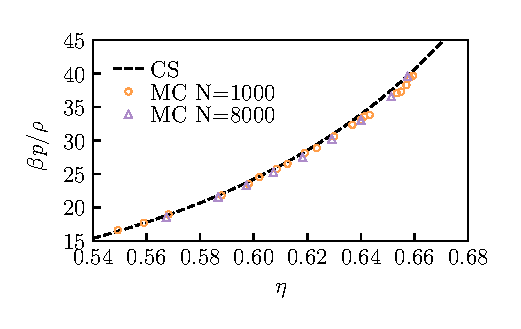
\includegraphics[width=0.9\linewidth,outer]{swap-cs-santos}
  \caption[Accuracy of Carnahan-Starling equation at high densities]{
    Accuracy of empirical Carnahan-Starling (CS) equation of state \eqref{eq:cs-mixtures} in the supercooled regime from comparison with novel Monte-Carlo (MC) simulations for a system with 23\% polydispersity.
    The size distribution of this system is described by \eqref{eq:berthier-size-measure}.
    The range of jamming volume fractions $\eta_J$ from non-equilibrium compression protocols with this system are indicated by the blue region.
    Simulation data and jamming densities reproduced from Ref.\ \cite{BerthierPRL2016}.
  }
  \label{fig:swap-eos}
\end{SCfigure}

Finally, we introduce the central approximation of chapters \ref{chapter:morphometric-framework}, \ref{chapter:morphometric-applications} and \ref{chapter:resummation} as a limit case of FMT.
The chemical potential of a new sphere $s$ can be determined as the free energy of a mixture where the limit where the new species is infinitely dilute, as in
\begin{equation}\label{eq:fmt-morphometric}
  \begin{split}
    \mu_s
    &=
    \lim_{\rho_s \to 0} \frac{\partial f^\mathrm{ex}}{\partial \rho_s}
    =
    \lim_{\rho_s \to 0}
    \sum_\alpha
    \frac{\partial n_\alpha}{\partial \rho_s}
    \frac{\partial f^\mathrm{ex}}{\partial n_\alpha},
    \\ &=
    \frac{\partial f^\mathrm{ex}}{\partial \xi_3} \frac{4 \pi R_s^3}{3}
    + \frac{\partial f^\mathrm{ex}}{\partial \xi_2} 4 \pi R_s^2
    + \frac{\partial f^\mathrm{ex}}{\partial \xi_1} R_s
    + \frac{\partial f^\mathrm{ex}}{\partial \xi_0}
  \end{split}
\end{equation}
using the explicit derivatives \eqref{eq:fmt-n-derivatives} in the second line.
Noting that the partial derivatives of $f^\mathrm{ex}$ are constants of the bulk liquid and the other contributions are normalisations of the intrinsic volumes (cf.\ Table \ref{table:geometric-quantities}), the central conjecture of the morphometric approach is that this generalises to arbitrary shapes; that is, the chemical potential can be written \cite{KonigPRL2004,RothPRL2006}
\begin{equation}\label{eq:fmt-morphometric-2}
  \mu_s = p V_s + a_2 A_s + a_1 R_s + a_0
\end{equation}
with thermodynamic coefficients $\{p, a_2, a_1, a_0\}$ independent of the geometry.
We leave detailed discussion of this approximation until chapter \ref{chapter:morphometric-framework}, but for reference we will give the explicit coefficients for the already introduced FMT functionals below.

The thermodynamic coefficients in \eqref{eq:fmt-morphometric-2} can be determined for an FMT functional using the special case of spherical solutes \eqref{eq:fmt-morphometric}.
For the Rosenfeld functional \eqref{eq:rosenfeld-functional} we obtain the thermodynamic coefficients for the single-component hard sphere liquid
\begin{subequations}\label{eq:rosenfeld-coefficients}
  \begin{align}
    \beta a_0^\mathrm{RF}
    &=
    -\ln{(1- \eta)},
    \\
    \beta a_1^\mathrm{RF}
    &=
    \frac{6\eta}{\sigma (1 - \eta)},
    \\
    \beta a_2^\mathrm{RF}
    &=
    \frac{6\eta + 3\eta^2}{2\pi \sigma^2 (1 - \eta)^2},
    \\
    \frac{\beta p^\mathrm{RF}}{\rho}
    &=
    \frac{1 + \eta + \eta^2}{(1 - \eta)^3}.
    \label{eq:py-pressure}
 \end{align}
\end{subequations}
and for the CS functional \eqref{eq:santos-fmt} with \eqref{eq:cs-fmt} we find
\begin{subequations}\label{eq:wbii-coefficients}
  \begin{align}
    \beta a_0^\mathrm{WBII}
    &=
    - \ln{(1 - \eta)},
    \\
    \beta a_1^\mathrm{WBII}
    &=
    \frac{2}{\sigma} \left(
    \frac{5\eta + \eta^2}{1 - \eta}
    + 2 \ln{(1 - \eta)}
    \right),
    \\
    \beta a_2^\mathrm{WBII}
    &=
    \frac{1}{\pi \sigma^2} \left(
    \frac{\eta (2 + 3\eta - 2\eta^2)}{(1 - \eta)^2}
    - \ln{(1 - \eta)}
    \right),
    \\
    \frac{\beta p^\mathrm{WBII}}{\rho}
    &=
    \frac{1 + \eta + \eta^2 - \eta^3}{(1-\eta)^3},
 \end{align}
\end{subequations}
We label these as the White Bear II (WBII) coefficients because they were first derived from the WBII free energy functional%
\marginfootnote{These are not exactly as stated in Ref.\ \cite{Hansen-GoosJPCM2006} because we use a different definition of surface.
  The conversions between the different surfaces are stated in chapter \ref{chapter:morphometric-framework}: see the discussions around \eqref{eq:exclusion-transform}.}
\cite{Hansen-GoosJCP2006, Hansen-GoosJPCM2006} which is similar in form and construction to the CS functional described, although it is (marginally) less self-consistent.

%% \subsection{Superposition and convolution approximations}

%% \todo{Finish this section}
%% In the Kirkwood superposition approximation \cite{KirkwoodJCP1935} many-body correlations are expressed as pairwise products of the two-body correlation function, i.e.
%% \begin{equation}
%%   g^{(n)}(\vec{r}^n) =
%%   \prod_{i < j} g^{(2)}(\vec{r}_i, \vec{r}_j),
%% \end{equation}
%% which correctly satisfies the hard-core condition, but violates the sum rule
%% \begin{equation}
%%   \begin{aligned}
%%     \rho^{(n)}(\vec{r}^n) &=
%%     \frac{1}{\Xi} \sum_{N=n}^\infty \frac{z^N}{(N-n)!} \int e^{-\beta U_N} \, d\vec{r}^{(N-n)} \\
%%     &=
%%     \int d\vec{r}_n \left(
%%     \frac{1}{\Xi} \sum_{N=n}^\infty \frac{z^N}{(N+1 - (n+1))!} \int e^{-\beta U_N} \, d\vec{r}^{(N-(n+1))}
%%     \right) \\
%%     &=
%%     \int d\vec{r}_n \left(
%%     \frac{1}{\Xi} \sum_{N=n}^\infty \frac{z^N}{(N - (n+1))!} \int e^{-\beta U_N} \, d\vec{r}^{(N-(n+1))}
%%     \right) \\
%%     &=
%%     \frac{1}{N-n}
%%     \int \rho^{(n+1)}(\{\vec{r}^n, \vec{r}_{n+1}\}) d\vec{r}_{n+1},
%%   \end{aligned}
%% \end{equation}\todo{This is wrong.}
%% and the related convolution approximation \cite{JacksonRMP1962,IchimaruPRA1970,BarratMP1988}%
%% \todo{Check this expression is correct - it almost certainly is not.}
%% \begin{equation}
%%   S^{(n)}(\vec{k}^n) =
%%   (1 + \widetilde{c}^{(n)}(\vec{k}^n))
%%   \prod_{i < j} S^{(2)}(\vec{k}_i, \vec{k}_j)
%% \end{equation}
%% satisfies the sum rule but fails to satisfy the hard-core condition.

%% In equilibrium
%% \begin{equation}
%%   c^{(n)}(\vec{r}^n) =
%%   \left.
%%   \frac{\delta^n \beta F_{ex}}{\delta \rho(\vec{r}_1)\delta \rho(\vec{r}_2) \cdots \delta \rho(\vec{r}_n)}
%%   \right|_{\rho(\vec{r})=\rho}
%% \end{equation}

\section{Approaching high densities: supercooled liquids and glasses}
\label{sec:glass}

%% \subsection{Mean-field picture}
%% The infinite dimensional limit $d \to \infty$.

%% \subsection{Random first-order transition theory}
%% Perturbation from mean-field in $1/d$.

%% \subsection{Alternative pictures in physical dimensions}
%% For $d \le 3$
%% \subsubsection{Frustration-limited domain theory}
%% \subsubsection{Dynamical theories}

%% \subsection{Old intro stuff}

%% It is widely reported that glass is actually liquid, and as evidence of this the thickness of old windows at the bottom is pointed to.
%% This is actually a matter of some dispute, but contains a grain of truth.
%% Pre-modern methods of creating window glass involved spinning molten glass on magma to flatten it out.
%% Centrifugal forces caused the glass to be thicker on the outer disc, so panes of glass would always be heavier in one direction%
%% \marginfootnote{And personally, if I were setting an uneven pane of glass I would place the thicker and heavier part at the bottom.}.

%% To a soft matter physicist glass is a broader term, referring to a wide class of materials while the window glass of common parlance is referred to by its chemical name \emph{silicate}.
%% This class of materials share many features of being disordered etc \cite{?} although in some sense they are connected by what they do \emph{not} do: which is flow on human timescales.
%% When I refer to `glass' I will be using it in this broad technical sense of a state of matter.
%% Some examples besides silicate:
%% \begin{itemize}
%% \item Most of the ice in the universe exists in an amorphous state in comets \cite{?}
%% \item Ceramics
%% \item Plastics: amorphous polymers
%% \end{itemize}
%% Of more abstract nature which could be called glassy though they are not materials
%% \begin{itemize}
%% \item Gels: super glasses, liquid like bit plus a network/backbone which has glassy dynamics
%% \item Neural networks
%% \item Non-deterministic polynomial time (NP) problems
%% \end{itemize}
%% We will not be directly addressing the latter type of more abstract problems which could be considered glasses, although they are arguably related due to a similar underlying disorder.
%% We will be focusing on only the most rudimentary of glassy phenomenology: the dynamical arrest of liquids at high densities/low temperatures when crystallisation is avoided.
%% Especially as it manifests in hard spheres, which as discussed is the reference system of choice for simple liquids.

%% Personally, the observation that got me interested in the field is the entropy argument.
%% If one compares the difference between the entropy of the crystal and the glass, and extrapolates wildly one expects there to be a point where the glass has a lower entropy than the crystal.
%% This is not very meaningful by itself, as we have already established by discussing the crystal vibrational entropy can be quite subtle so it is possible for the liquid to have a lower vibrational entropy.
%% However, if one corrects this with more modern techniques to measure just the entropy corresponding to non-trivial motion we see that there is a point where the configurational (i.e.\ not purely vibrational) entropy vanishes: this would imply the system is frozen in a single configuration.
%% Such a point would define a transition to a genuine thermodynamic phase, an ideal glass.

%% Hard glasses: high elastic constants.
%% Colloidal suspensions: soft matter version, small elastic constants.
%% Same phenomenology though.
%% What is a glass?
%% Frozen in a (apparently) disordered state.
%% All sorts of glasses, structural, spin, orientational, electron, vortex.
%% Glasses formed by liquids, colloidal suspensions and polymers: traditional structural glasses.
%% Solid: doesn't flow on observational time, resists small/infinitesimal shear (acts like solid).
%% Amorphous, apparently amorphous: no periodic arrangement like in crystal.
%% Homogeneous makes useful for technology: useful for e.g.\ optical properties.

In the introduction we established the supercooled liquid in hard spheres as the extension of the stable liquid above the freezing density, where it is metastable to the crystal phase.
To provide proper context we will discuss supercooled liquids more generally here, including thermal systems where temperature is the more natural control parameter.
As such, we will be considering the effect of decreasing temperature on the supercooled liquid.

%First, we describe the phenomenology of supercooled liquids before delving into the specific theories to explain them.

\subsection{Properties of the supercooled liquid}

We will start by exploring the ways in which supercooled liquids are the \emph{same} as regular liquids, expanding in more detail on ideas discussed in the introduction.
Then we will move onto the ways in which they \emph{differ} from ordinary liquids, notably in their dynamical properties.

\begin{SCfigure}
  \missingfigure[figwidth=\linewidth]{$g^{(2)}$}%
  \caption[Structural change in the supercooled liquid (at the pair level)]{
    Minimal change in pairwise structure with increasing density above the melting point, as measured by the pair distribution function \eqref{eq:n-particle-distribution}.
  }
  \label{fig:g2-changes}
\end{SCfigure}

Structurally, supercooled liquids are not meaningfully different from their ordinary counterparts.
Operationally, a supercooled liqiud is equilibrated in the sense that all observables are time independent and the thermodynamics is self-consistent%
\marginfootnote{Different routes to measuring thermodynamic quantities, e.g.\ the pressure, may give different values in an out-of-equilibrium system.
  This is not the case in supercooled liquids, even though they are not strictly in equilibrium.}.
Formally speaking, the system is sometimes said to be in \emph{local equilibrium}, where it samples all the liquid microstates ergodically; or that it obeys \emph{detailed balance}, where the dynamics is microscopically reversible.
%have very similar structural characteristics as at equilibrium.
As a consequence, the liquid loses any memory of its preparation and all observables become time independent.
That is, for some observable $A$ we can write
\begin{equation*}
  \langle A(t) \rangle = \langle A \rangle.
\end{equation*}
This includes the static correlation functions, introduced in section \ref{sec:liquid-structure}, which remain well-defined in the supercooled regime.
Furthermore, the pair distribution function $g^{(2)}(r)$ is seen to change very little as the density (or temperature) is increased (decreased) from the normal liquid; as an example, we show this for hard spheres in Fig.\ \ref{fig:g2-changes}.
As pair correlations are the main measure of structure in simple liquids, this suggests minimal structural change occurs in the high density liquid.
As a corollary, time correlation functions become \emph{time-translation invariant} meaning they depend only on time differences i.e.\
\begin{equation*}
  \langle A(t) A(t') \rangle = \langle A(0) A(t - t') \rangle.
\end{equation*}

A more sophisticated way in which supercooled liquids can be thought of as equilibrium systems involves the response functions.
In an equilibrium system, the response of a system to a small perturbation is directly related to the microscopic source of fluctuations%
\marginfootnote{Temperature, in the case of liquids.}.
The \emph{fluctuation-dissipation relation} for an observable $A$ expresses the system's susceptibility to perturbation as
\todo{Check this equation is correct against a textbook, get a citation.}
\begin{equation*}
  \chi_A (t, t')
  =
  - \beta \Theta(t - t')
  \frac{d}{dt}
  \left(
  \bigg\langle
  (A(t - t') - \langle A \rangle)
  (A(0) - \langle A \rangle)
  \bigg\rangle
  \right)
\end{equation*}
where the Heaviside theta function imposes causality.
These relations are obeyed in supercooled liquids, even though they are not a proper equilibrium state.

Now we turn to discussing the ways in which supercooled liquids are markedly different from normal liquids: in their \emph{dynamics}.
Typically this is discussed in the context of two (related) quantities: the \emph{viscosity} and the \emph{relaxation time}.
Viscosity measures how resistant the system is to flow, while relaxation time measures the typical microscopic time for the density profile to relax i.e.\ for liquid-like behaviour caused by particle diffusion.
A defining feature of supercooled liquids is that these numbers become so large that the precise details of the measurement used does not matter.
We will discuss this dynamical slowdown further on, but for now we introduce a specific time correlation function in order to frame the discussion.
A popular measurement is the (self) intermediate scattering function (ISF), defined by \cite{JanssenFP2018}
\begin{equation}\label{eq:isf}
  F(k, t)
  =
  \frac{
    \big\langle \tilde{\rho}(\vec{k}, t) \tilde{\rho}(-\vec{k}, 0) \big\rangle
  }{
    \langle N \rangle
  }
\end{equation}
which reduces to the static structure factor \eqref{eq:static-structure-factor} at zero elapsed time $F(k, t=0) = S^{(2)}(k)$.
An example ISF is shown in Fig.\ \ref{fig:isf}, displaying many features emblematic of the supercooled liquid which distinguishes it from the regular liquid.
\hl{describe the features, introduce alpha relaxation time}

\begin{SCfigure}
  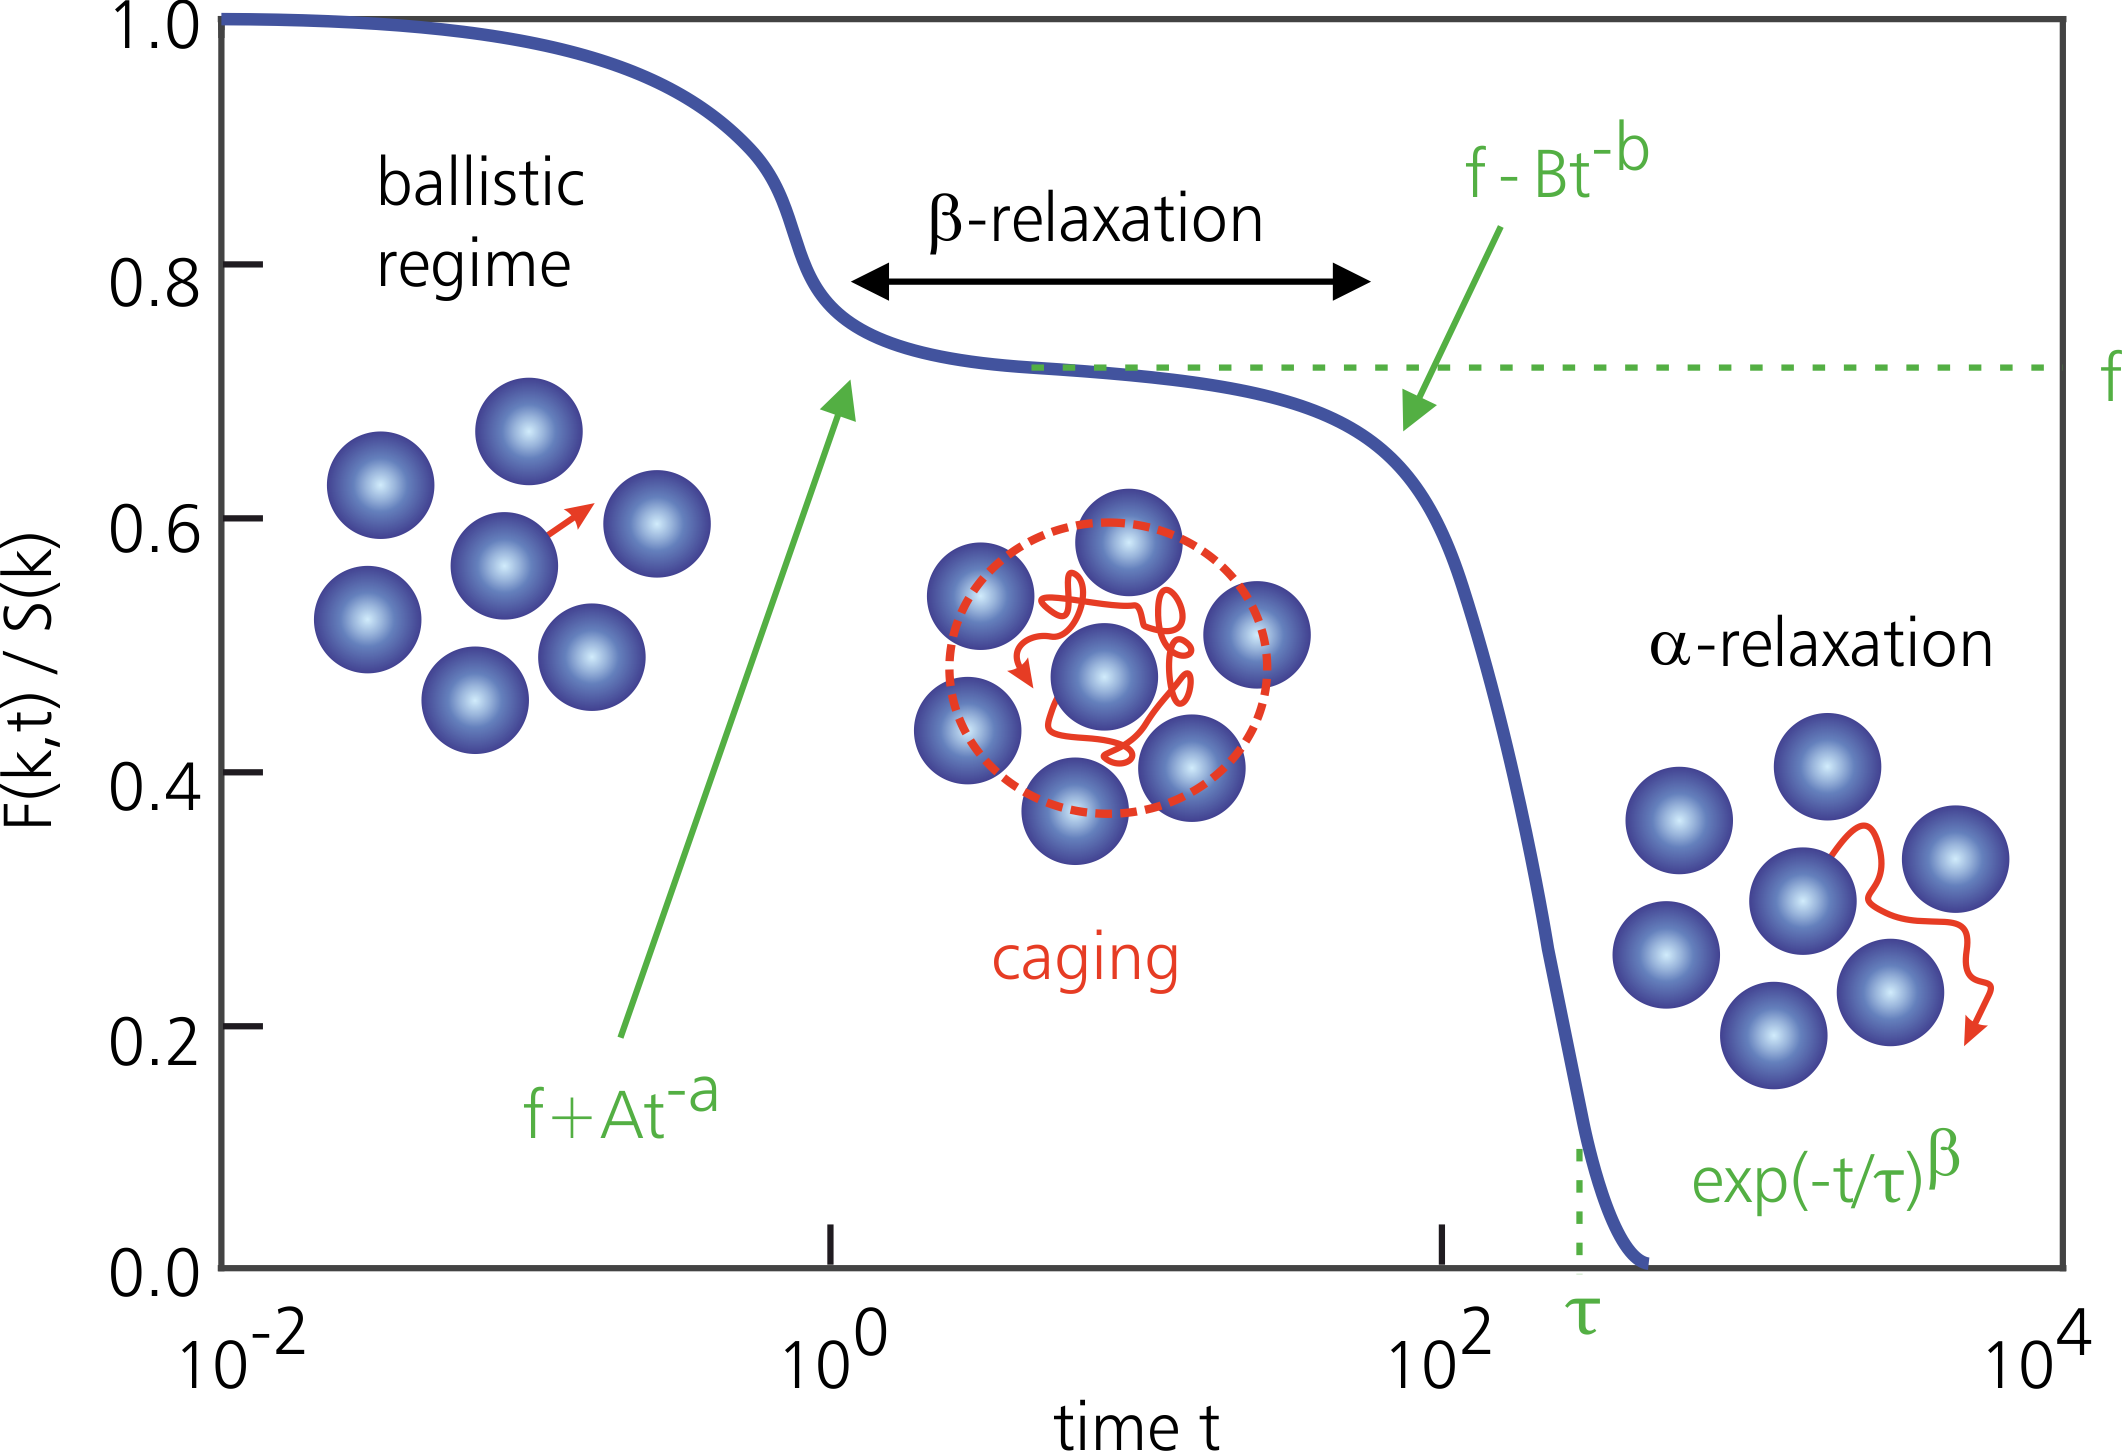
\includegraphics[width=0.9\linewidth,outer]{isf}
  \caption[Intermediate scattering function in a supercooled liquid]{
    Typical intermediate scattering function in a supercooled liquid.
    The power law predictions are from mode-coupling theory.
    Reproduced from Ref.\ \cite{JanssenFP2018}.
  }
  \label{fig:isf}
\end{SCfigure}

A helpful framework to guide discussion of dynamical processes is \emph{transition state theory}.
In this approach a dynamical process, e.g.\ a chemical reaction, is imagined to occur through a dynamical bottleneck (Fig.\ \ref{fig:transition-state}).
We imagine evaluating a thermodynamic potential%
\marginfootnote{Which thermodynamic potential this corresponds to will depend on the ensemble.}
$\Phi$ at every point along the reaction path.
The process will then be limited by the rate of thermal fluctuations of size $\Delta \Phi$, i.e.\ those able to reach the transition state.
In equilibrium, the timescale for the process will then scale by the Boltzmann weight
\begin{equation}\label{eq:reaction-time}
  \tau \sim e^{\beta \Delta \Phi}.
\end{equation}
There will be additional kinetic prefactors out in front, however for large barriers we expect the thermodynamic contribution to dominate because of its exponential weighting.
This framework can be more rigorously justified through e.g.\ an \emph{instanton} approach \cite{LangerAP1969}.
The main limitation of transition state theory is the assumption that dynamical processes occur through effectively one-dimensional reaction paths; later, we will introduce a more sophisticated form of this framework which considers the high dimensional \emph{energy landscape}.

As an example of how useful transition state theory can be, we very briefly consider \emph{classical nucleation theory} which we will return to in more detail in chapter \ref{chapter:aerosols}.
Imagining crystallisation to occur by the spontaneous formation of the new phase inside of the liquid, then the timescale for this process will scale as
\begin{equation*}
  \tau_\mathrm{crys} \sim e^{ \beta \Delta \Phi_\mathrm{crys}}.
\end{equation*}
Then, assuming a temperature-independent barrier $\Delta \Phi_\mathrm{crys}$, the timescale for nucleation will increase exponentially as temperature is lowered allowing for the supercooled liquid to become long-lived \cite{CavagnaPR2009}.
%This is essentially the reason it is possible for supercooled liquids to exist at all, and reach an effectively time-translation invariant state without decaying to the crystal \cite{CavagnaPR2009}.
This argument is highly system dependent, as systems with small barriers to crystallisation will not be long-lived enough for a metastable supercooled phase to be observed.
Single-component hard spheres are particularly prone to crystallise at very high densities, so polydispersity is typically introduced to frustrate the crystal structure and extend the lifetime of the supercooled liquid.
This is an imperfect process however, as even highly polydisperse systems have been found to crystallise \cite{BommineniPRL2019,BerthierPRL2016}.

\begin{SCfigure}
  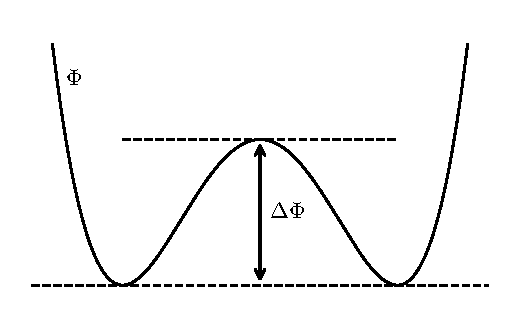
\includegraphics[width=0.7\linewidth,center]{transition-state}
  \caption[Transition state theory]{
    A double-well potential featuring a barrier $\Delta\Phi$, representing the minimum energy required for the system to pass between the two \emph{basins}.
    The $x$-axis is the \emph{reaction coordinate}, representing a one-dimensional projection of the complete degrees of freedom.
  }
  \label{fig:transition-state}
\end{SCfigure}

Applying transition-state theory \eqref{eq:reaction-time} to relaxation time in the liquid, we may expect the alpha relaxation time to scale as
\begin{equation}\label{eq:tau-barrier}
  \tau_\alpha \sim e^{\beta \Delta \Phi_\alpha}
\end{equation}
where $\Delta \Phi_\alpha$ is the barrier to relaxation.
Naively, we might expect the barrier to remain constant with temperature, corresponding to e.g.\ the cost of breaking a chemical bond, then we arrive at the Arrhenius law
\begin{equation}\label{eq:arrhenius-law}
  \ln{\tau_\alpha} \propto \frac{1}{T}.
\end{equation}
This argument captures the high temperature behaviour very well and, outside of soft matter, it applies reasonably well to molecular glassformers e.g.\ silica-based materials%
\marginfootnote{That is, the material which the average person would mean when they say ``glass''.},
where relaxation essentially depends on the timescale to break a covalent bond.
Experimental data \hl{(citation)} for \ce{SiO2} confirms that $\ln{\tau_\alpha}$ scales linearly with $\beta$ (Fig.\ \ref{fig:angell}).
By convention, systems which scale in an Arrhenius fashion are called \emph{strong}%
\marginfootnote{This baffling naming convention has nothing to do with the mechanical properties.}
glassformers.

Our focus is on soft matter, with hard spheres as the prototypical model, where the  chemical bonds (typically van der Waals attractions) are much weaker than in molecular systems.
Consequently, there is less of a case for an Arrhenius relationship \eqref{eq:arrhenius-law}, and empirically we find striking deviations from it.
Many systems show \emph{super-Arrhenius} scaling with temperature (Fig.\ \ref{fig:angell}), including mixtures of Lennard-Jones atoms and molecular orthoterphenyl.
Correspondingly, systems scaling faster than exponentially are labelled as \emph{fragile}.

Some modification is required for hard particle systems, where temperature is not a natural control parameter.
As we argued in the introduction, pressure is the only meaningful state variable.
The authors of Ref.\ \cite{BerthierPRE2009} argue that pressure plays a role equivalent to inverse temperature in athermal systems, because of similarities in their limit behaviour.
Alternatively, we could make a free volume argument, where we expect a relaxation event to involve fluctuations of volume $\Delta V$.
In equilibrium, volume fluctuations are created by reversible work $p \Delta V$ so to leading order%
\marginfootnote{The leading order behaviour can be given more justification by invoking the morphometric approach \eqref{eq:fmt-morphometric-2}, or from more general arguments which we will introduce in section \ref{sec:insertion-as-solvation}.}
we then expect
\begin{equation*}
  \tau_\alpha \sim e^{\beta p \Delta V}.
\end{equation*}
Taking $\Delta V$ as the equivalent of an energy barrier, we find the conjugate variable $\beta p$ does indeed play the role of inverse temperature.
It is usual to work with the dimensionless \emph{compressibility factor}, defined by
\begin{equation}
  Z = \frac{\beta p}{\rho},
\end{equation}
in terms of which hard spheres show the same phenomenology as thermal systems in Fig.\ \ref{fig:angell}.
We find hard spheres are comparable in fragility to various binary Lennard-Jones mixtures.

\hl{Things I have not yet mentioned:}
\begin{itemize}
\item \hl{glass transition: 100s}
\item \hl{operationally, what it looks like in thermodynamic potentials as the system falls out of equilibrium.}
\item \hl{dynamical heterogeneities (can probably save this until mentioning facilitation though)}
\item \hl{Stokes-Einstein breakdown}
\end{itemize}

%% We discussed the static correlation functions at length, which is fine for liquids where equilibrium occurs on a \SI{100}{\pico\second} timescale.
%% Dynamical effects are highly nontrivial at high densities.
%% As a practical definition, a glass is defined in the lab as any material for which the relaxation time exceeds \SI{100}{\second}: this point is called the experimental glass transition.
%% This is somewhat arbitrary, although the location of the glass transition point is not particularly sensitive to where you set the threshold because of how rapidly the viscosity/times are increasing around there.
%% So what do we mean by dynamical arrest.

%% Cooling a liquid.
%% Take thermodynamic quantity (e.g.\ volume, entropy, enthalpy): usually crystallise.
%% (Picture)
%% First-order transition bypassed by quick cooling.
%% Enter supercooled liquid phase.

%% Both of these conditions are violated in the glass, as this is a truly non-equilibrium state.
%% That is, we see ageing, and hysteresis in response to perturbations.
%% No longer equilibrates/relax/flows, call it a glass: occurs at glass transition.
%% Glass is a solid for all practical purposes.
%% Distinguished from glass which has dependence on preparation history, hysteresis/memory effect of heating the system (will not follow exactly the same curve until - back to the equilibrium supercooled structure), aging: averages (including correlations) evolve in time.

%% The glass transition itself is not a ``transition'' in the thermodynamic sense; there is no.
%% It's really a kind of impatience transition; the glass transition for a human would be different to the glass transition for a demigod/ent.
%% It's still a relatively robust measurement, because of the superarrhenius scaling (sc-l for pedestrians).

%% A plethora of questions related to the out-of-equilibrium properties.
%% \begin{enumerate}
%% \item Properties of out of equilibrium glass phase: very important questions for material science. Low temperature anomalies, aging behaviour, nonlinear rheology  plasticity.
%% \item Relation between glass and jamming. Jamming=zero temperature, out of equilibrium, infinite pressure.
%% \item How to avoid crystallisation.
%% \end{enumerate}

A super-Arrhenius scaling of $\tau_\alpha$ implies that the thermodynamic barrier itself $\Delta \Phi_\alpha$ increases with supercooling.
This means that the dynamics fundamentally changes at high densities (or low temperatures), which must be caused by the onset of \emph{collective} effects%
\marginfootnote{Also referred to as \emph{cooperative} effects.};
given the weakness of bonds in soft matter, we can conclude that many particles must contribute to create a large barrier.
We will discuss this more in the next section.
Relaxation barriers in hard spheres are entropic in nature, so perhaps it is easier to see the need for collective effects.
Moreover, the geometrical interpretation in terms of volume fluctuations $\Delta V$ provides a picture for collective motion: at high densities more particles will have to move out of the way to create the space for motion.

\begin{SCfigure}
  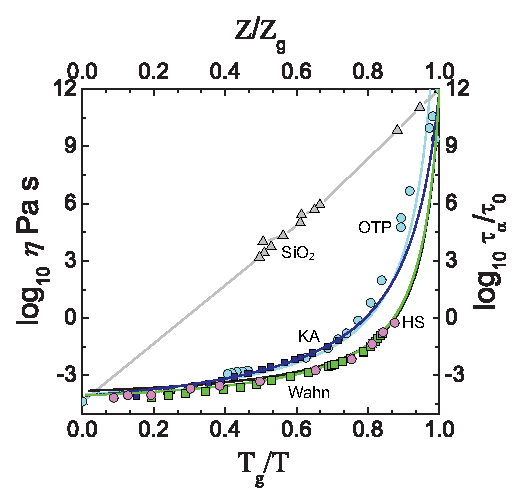
\includegraphics[width=0.9\linewidth,outer]{angell}
  \caption[Angell plot]{
    The \emph{Angell} plot for molecular and model glassformers showing the temperature/pressure dependence of viscosity $\eta$ (or equivalently relaxation time $\tau_\alpha$).
    The molecular systems \ce{SiO2} and orthoterphenyl (OTP) respectively display the \emph{strong} and \emph{fragile} behaviours described in text.
    Kob-Anderson (KA) and Wahnstrom (Wahn) are binary mixtures of Lennard-Jones atoms designed to exhibit fragility.
    The compressibility $Z = \beta p / \rho$ is argued to be equivalent to inverse temperature for hard spheres (HS) \cite{BerthierPRE2009}.
    Reproduced from Ref.\ \cite{RoyallPR2015}.
  }
  \label{fig:angell}
\end{SCfigure}

%% We will talk about this metastable branch as if it were in equilibrium.
%% \todo{create link when mention high density swap data}

%% Relationship with viscosity.
%% Flowing/not flowing is captured by viscosity: viscous slowdown same as relaxation slowdown.
%% Slightly different notion.
%% Short times $t \ll \tau$: elastic system, long times $t \gg \tau$: viscosity.
%% Time barrier is relaxation time.
%% Elasticity, viscosity in Newtonian fluids: viscoelastic behaviour (Maxwell)
%% \begin{equation}
%%   \eta = G_\infty \tau_\mathrm{relax}
%% \end{equation}
%% high frequency shear modulus is elastic property.
%% Shear modulus increases by factor 2-5 times, is dwarfed by change in relaxation time.

\subsection{Mode-coupling theory}

Reviews: \cite{ReichmanJSM2005, JanssenFP2018}

We start with an explicitly dynamical theory.
Central idea: \emph{slow} and \emph{fast} variables.

To motivate mode-coupling theory we start from the classical Langevin equation of motion, which expresses the equations of motion of a subset of the degrees of freedom.
Newton's equation becomes
\begin{equation*}
  m \ddot{\vec{r}} = - \lambda \dot{\vec{r}} + \vec{F}(t)
\end{equation*}
where $\vec{F}$ is a Gaussian random field
\begin{equation*}
  \langle F_i(t) F_j(t') \rangle = 2 D \delta_{i,j} \delta(t - t').
\end{equation*}
This equation is valid where there is a timescale separation between \emph{slow} and \emph{fast} variables: the position $\vec{r}$ represents a slowly evolving variable of interest, whereas the remaining degrees of freedom (e.g.\ small solvent particles) are imagined to equilibrate rapidly leaving only the force field $\vec{F}$.

In mode-coupling theory, an \emph{exact} generalised Langevin equation is derived as
\begin{equation}
  \frac{d \vec{x}(t)}{dt}
  =
  i \vec{\Omega} \cdot \vec{x}
  - \int_0^t \vec{K} \cdot \vec{x}(t - t') \, dt'
  + \vec{f}(t)
\end{equation}
where $\vec{\Omega}$ is frequency matrix, $\vec{K}$ is a time-dependent \emph{memory function}, and $\vec{f}$ is the fast fluctuating force.

The full MCT equation
\begin{equation}
  \frac{d^2 F(k,t)}{d t^2}
  + \frac{k^2}{\beta m S(k)} F(k, t)
  + \int_0^t K_\mathrm{MCT}(k, t') \frac{d F(k, t - t')}{dt} \, dt'
  =
  0
\end{equation}
with the memory function given by
\begin{equation}
  K_\mathrm{MCT}
  =
  \frac{\rho}{16 \pi^3 \beta m}
  \int |V_{\vec{q},\vec{k}-\vec{q}}|^2
  F(q, t) F(|\vec{k} - \vec{q}|, t)
  \, d\vec{q}.
\end{equation}

Predicts a diverging timescale.
Nevertheless, liquids can be prepared above this volume fraction in colloidal experiments \cite{BrambillaPRL2009} and simulations \cite{BerthierPRL2016}.

The point of this section is to indicate that pair correlation functions are not enough.
Extensions with higher order structure \cite{JanssenPRL2015,JanssenFP2018}.

\subsection{Mean-field theory}

A growing consensus is forming around this explanation.
Inspired by the solutions of mean-field spin glasses, the great breakthrough of the original papers was that these systems were identical in the structure of the energy landscape.
Connection between thermodynamics and dynamics, configurational entropy.
This argument is thermodynamic, which in some sense is structural.
Structural in the sense of the energy landscape, not necessarily in real space/local structure.
Compatible with MCT, in fact high dimensional calculations lead to a theory almost identical to MCT \cite{MaimbourgPRL2016,KurchanJSM2016}.

The relevance of mean-field theory in physical dimensions comes from an interpretation \cite{KirkpatrickPRB1987, KirkpatrickPRA1989}, and antecedent ideas found in \cite{AdamJCP1965}.
RFOT: argument of Ref.\ \cite{BouchaudJCP2004}, introduces point-to-set length.

Point-to-set length is the minimum size of a subsystem for there to be relaxation: the space of states transitions from being a single state (point) to a multitude of states (set).
It can be rigorously proven that a diverging timescale necessarily must coincide with a diverging point-to-set length: Montanari \cite{MontanariJSP2006}.
The essence of the argument is that for a finite subsystem, there will be a finite barrier, so any dynamics must scale Arrheniusly.
Therefore, the relaxation time will be bounded from above by the dynamical lengthscale, and super-Arrhenius scaling suggests growing collective behaviour.

This must trivially occur at the very least $T=0\si{K}$ where relaxation timescales diverges, however much like the lack of a phase transition in the Ising model in $d=1$ this is not a true thermodynamic phase transition because it cannot be crossed.
Recent numerical evidence suggests that a model glassformer in $d=2$ does not show a transition, also vanishing at $T=0\si{K}$ \cite{BerthierNC2019}.
So the central question of glass is what happens in $d=3$, is there a vanishing configurational entropy at a finite $T > 0$ with an accompanying thermodynamic glass transition?
In mean-field, formally in the limit of infinite spatial dimensions $d \to \infty$, the hard sphere system has been shown to have a true transition, however the critical dimensions are unknown so it is unclear what happens in $d=3$. \cite{KurchanJSM2012,KurchanJPCB2013,CharbonneauNC2014,CharbonneauJSM2014}.

\begin{SCfigure}
  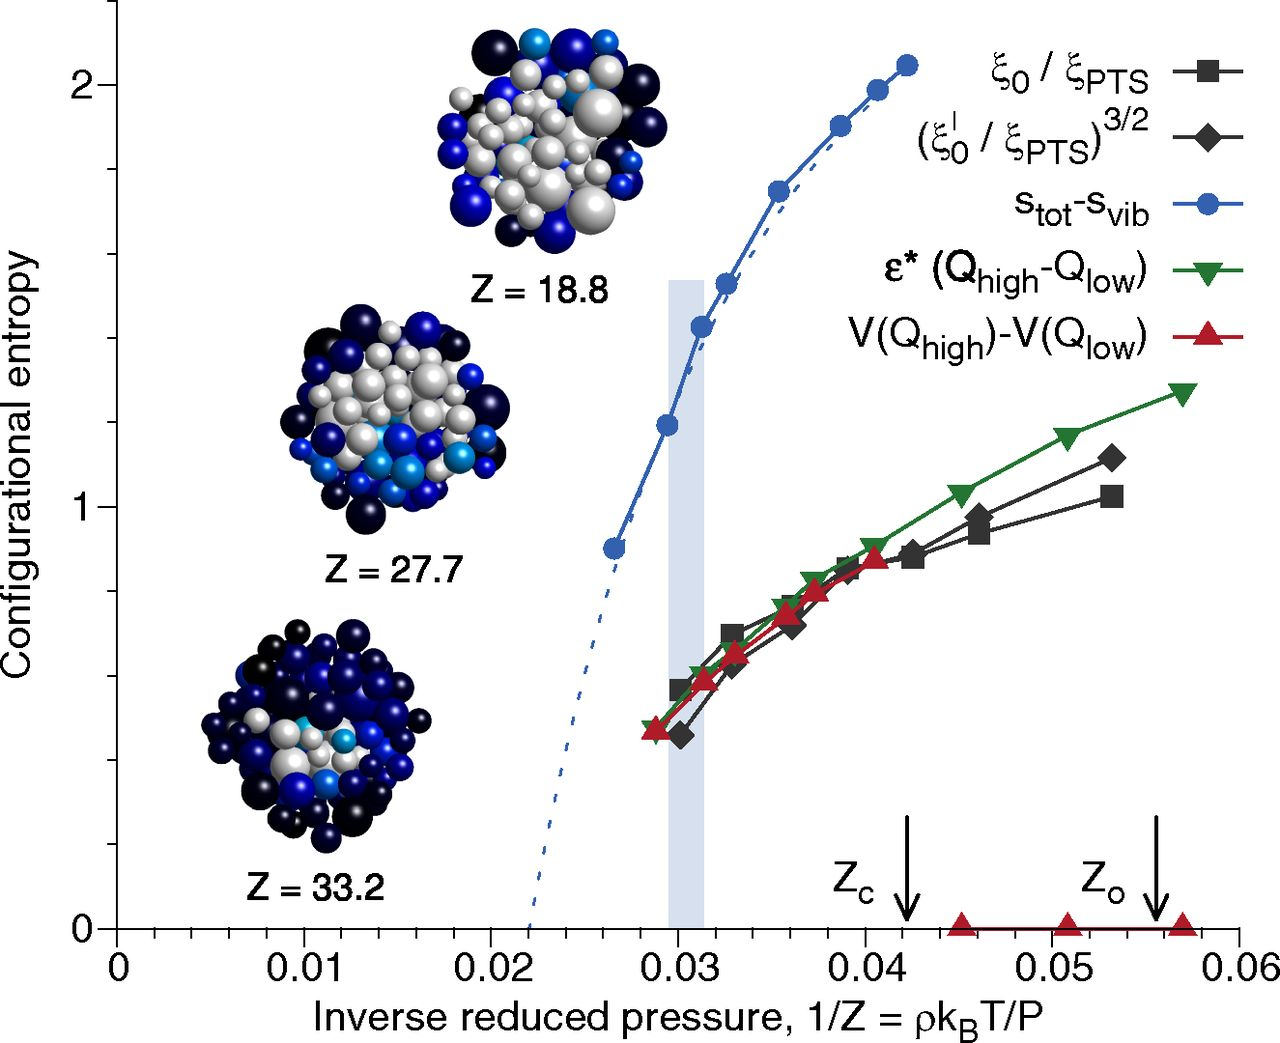
\includegraphics[width=0.9\linewidth,outer]{swap-Sconf}
  \caption[Configurational entropy in hard spheres from Monte-Carlo simulations]{
    Configurational entropy in hard spheres from novel Monte-Carlo (MC) simulations for a system with 23\% polydispersity.
    The various methods used (described in Ref.\ \cite{BerthierPNAS2017}) all broadly agree that this quantity is trending to zero at a finite pressure, suggesting the existence of a thermodynamic glass transition.
    The equation of state for this system is given in Fig.\ \ref{fig:swap-eos}.
    Reproduced from Ref.\ \cite{BerthierPNAS2017}.
  }
\end{SCfigure}

\subsection{Local structure picture}

Stripmine Paddy's review for this section \cite{RoyallPR2015}.

In conventional condensed matter physics dynamics is determined by structure.
For example, crystalline solids are fixed on a lattice so do not flow, whereas liquids are disordered and are thus able to flow.
Soft matter systems (e.g.\ gels, foams, glasses) do not neatly fall into this paradigm: their dynamics are often arrested whilst their structure remains highly disordered.

Frustration-limited domain theory \cite{TarjusJPCM2005}.

Previous viewpoints, MCT and mean-field, are structural in the sense of being thermodynamic; however they do not explicitly invoke local structure.
That being said, they are broadly compatible viewpoints.
After all, emergence of a structural motif would be sufficient to reduce the configurational entropy (or a manifestation of this, depend on one's viewpoint).

Glotzer picture: competition between competing structures \cite{TeichNC2019}.

\subsection{Other viewpoints: jamming and facilitation}

Theories concentrating on the high density glass: elastic theories.
Dynamic facilitation.

\subsection{Perspective: role of many-body correlations}

To motivate the use of many-body correlations we employ an argument due to Evans \cite{EvansPrivate2019}.
In section \ref{sec:thermodynamic-routes} we saw how the compressibility and virial routes lead to expressions of the free energy in terms of pair correlations.
This is emblematic of conventional routes to the free energy, so in some sense all of the thermodynamically relevant information is contained in the two body correlation functions.
However, the pair correlation yields thermodynamic quantities which are \emph{derivatives} of the free energy at an instantaneous state point, so to infer the free energy we must sample multiple state points.
Equivalently, we could consider the derivatives of the pair correlation function.
It is straightforward to show that \cite{Santos2016}
\begin{equation}\label{eq:correlation-derivatives}
  \chi_T \rho
  \left( \frac{\partial \rho^{(n)}}{\partial \rho} \right)_{V,T}
  =
  (n - \rho V) \rho^{(n)}(\vec{r}^n)
  + \int \rho^{(n+1)}(\vec{r}^{n+1}) \, d\vec{r}_{n+1}.
\end{equation}
The important feature to take away from this expression is the presence of $\rho^{(n+1)}$; we see that higher-order correlations emerge in the derivatives.
This means we could in principle measure the free energy at a single state point by introducing highly accurate measurements of the many-body correlation functions.
This is essentially the spirit of the \emph{entropy route}, which writes \cite{WallaceJCP1987}
\begin{equation}
  S = \sum_{n=1}^\infty S_n
\end{equation}
with entropic terms $S_n$ containing contributions from $n$-particle correlations.
The first few terms are given by \cite{WallaceJCP1987}
\begin{subequations}
  \begin{align}
    \frac{S_1}{V}%\langle N \rangle}
    &=
    k_B \, \rho \left( \frac{d}{2} - \ln{\rho \Lambda^d} \right),
    \\
    \frac{S_2}{V}%\langle N \rangle}
    &=
    \frac{\rho^2}{2 T}
    \int g^{(2)}(\vec{r}) \ln{g^{(2)}(\vec{r})}
    \, d\vec{r},
    \\
    \frac{S_3}{V}%\langle N \rangle}
    &=
    \frac{\rho^3}{6 T}
    %\int g^{(3)}(\vec{r}, \vec{r}') \delta w^{(3)}(\vec{r}, \vec{r}')
    \int g^{(3)}(\vec{r}, \vec{r}')
    \ln{\left(
      \frac{
        g^{(3)}(\vec{r}, \vec{r}')
      }{
        g^{(2)}(\vec{r}) g^{(2)}(\vec{r}') g^{(2)}(\vec{r} - \vec{r}')
      }
      \right)}
    \, d\vec{r} d\vec{r}'.
  \end{align}
\end{subequations}

Second, while it is true that thermodynamic quantities like the pressure can certainly be inferred from the pair correlations, there is no such simple relationship for dynamic quantities.
In the absence of a thermodynamic phase transition, we would not expect the pair correlation to reveal much about the nature of dynamical arrest, beyond the lack of a transition.
And even supposing the existence of a transition, the precision required to detect such a signal $g(r)$ may be arbitrarily subtle; however, any the changes approaching a transition \emph{must} be magnified in the higher order correlation functions because of \eqref{eq:correlation-derivatives}.
This is particularly true as we saw \hl{local mechanisms in the various theories}.

We will be focusing on many-body correlations in real space, to explore the local mechanisms proposed in theories of the glass transition mentioned above.
In some situations the correlations in Fourier space may be more useful, most notably in MCT where many-body generalisations have already found some traction \cite{JanssenPRL2015,JanssenFP2018}.
In principle, our real space correlation functions can be Fourier transformed to obtain these functions, but in practice this is prohibited by the high dimensionality of the correlation functions for even modest $n$.
However, we indicate below how FMT already provides an easy route to obtaining all the correlation functions in Fourier space, as described by the original papers \cite{RosenfeldPRL1989,RosenfeldJCP1990}.

Fourier transforming the direct correlation functions for the uniform liquid \eqref{eq:fmt-direct-correlations-uniform-density}, and applying the convolution theorem, allows us to write the rather succinct
\begin{equation}
  \tilde{c}^{(n)}(\vec{k}^n)
  =
  - \sum_{\alpha_1, \alpha_2, \cdots, \alpha_n}
  \partial^n_{\alpha_1, \alpha_2, \cdots, \alpha_n} \beta f^\mathrm{ex} \;
  \left( \prod_{i=1}^n \widetilde{\omega}_{\alpha_i}(\vec{k}_i) \right)
  \delta(\vec{k}_1 + \vec{k}_2 + \cdots + \vec{k}_n).
\end{equation}
The delta function enforces the `ring' condition $\sum_{i=1}^n \vec{k}_i = 0$ which emerges from translational symmetry of the weight functions, reducing the dimensionality of the domain by $d$.
A further $d(d-1)/2$ degrees of freedom%
\marginfootnote{This many degrees of freedom can be removed for general $n \ge d$, but we expect fewer for $n < d$.
  For example, $n=2$ arrangements (a dimer) are isomorphic to a line so they possess $d-1$ rotational degrees of freedom.}
can be removed by exploiting rotational symmetry.
Many-particle generalisations of the static structure factor can be obtained from $\tilde{c}^{(n)}(\vec{k}^n)$ by functionally differentiating the Ornstein-Zernike equation \eqref{eq:ornstein-zernike-generic} with respect to density \cite{BarratMP1988}.

This concludes the relevant background on liquid state theory.
In subsequent chapters we will develop a framework for treating the (real space) many-body correlation functions.


\ifdefined\includebibliography
  \printbibliography
\fi

\end{document}

\documentclass[12pt]{report}
\usepackage{preamble}
\setcounter{chapter}{2}

\begin{document}
\chapter{Morphological framework for many-body correlations}
Mostly theoretical but with some numerical experiments which motivate/justify developments to the theory.
The main body of numerical work is left to the following chapter.

\section{Formalism for many-body correlations}

We write the $n$-particle distribution function $g^{(n)}$ as
\begin{equation}\label{eq:n-density-pdf}
  \textrm{Probability}\left( \textit{any } n \textrm{ particles in volume } d\vec{r}^n \right)
  \equiv
  \rho^n g^{(n)}(\vec{r}^n) \, d\vec{r}^n.
\end{equation}
In the main text, we expressed $g^{(n)}$ in terms of a generalised potential of mean force $\phi^{(n)}$: the reversible work required to insert $n$ particles into the liquid.
We decomposed $\phi^{(n)}$ into a local (potential energy) and solvent (free energy) component.
Although this quantity is quite intuitive and could be determined heuristically, here we give a short proof that this decomposition is formally exact and arises quite naturally from the definition of the distribution function.

In the grand-canonical ensemble the $n$-particle density $\rho^{(n)}(\vec{r}^n) \equiv \rho^n g^{(n)}$ is determined by integrating over the remaining degrees of freedom~\cite{Hansen2013}
\begin{equation}
  \rho^{(n)}(\vec{r}^n)
  = \frac{1}{\Xi} \sum_{N=n}^\infty \frac{z^N}{(N-n)!} \int e^{-\beta U_N} \, d\vec{r}^{(N-n)},
\end{equation}
where the activity is written in terms of the thermal de Broglie wavelength $\Lambda$ as $z = \exp{\beta\mu} / \Lambda^d$.
Changing the summation limits $N \rightarrow N+n$ we obtain
\begin{equation}\label{eq:n-density}
\begin{aligned}
  \rho^{(n)}(\vec{r}^n)
  &= \frac{z^n}{\Xi} \sum_{N=0}^\infty \frac{z^N}{N!} \int e^{-\beta U_{N+n}} \, d\vec{r}^{N} \\
 & = z^n e^{-\beta U_n} \left< e^{-\beta U_{n \leftrightarrow N}} \right>
\end{aligned}
\end{equation}
where in the latter step we decomposed the total potential $U_{N+n}$ into purely local and solvent terms, i.e.\ $U_{N+n} = U_n + U_N + U_{n \leftrightarrow N}$, where $U_\alpha$ for $\alpha \in \{n,N\}$ indicates the internal interactions between particles in component $\alpha$.
The ``interspecies'' interactions are contained within $U_{n \leftrightarrow N}$ which acts as an external field for the solvent.
The angled brackets indicate ensemble averaging over all arrangements of the solvent, i.e.\
\begin{equation}
  \left< \cdots \right> =
  \frac{1}{\Xi} \sum_{N=0}^\infty \frac{z^N}{N!} \int \left(\cdots\right) e^{-\beta U_N} \, d\vec{r}^N,
\end{equation}
with partition function of the unperturbed system $\Xi \equiv e^{-\beta \Omega_{hom}}$, where $\Omega_{hom} = -p V$ is the usual homogeneous grand potential.
Thus, \eqref{eq:n-density} becomes
\begin{equation}
  \rho^{(n)}(\vec{r}^n)
  = z^n e^{-\beta (U_n + \Omega - \Omega_{hom})}.
\end{equation}
where $\Omega$ is the grand potential of the solvent in the presence of the $n$-particle inhomogeneity.
Splitting the chemical potential into its ideal and excess parts so that $\beta\mu = \ln{\Lambda^d \rho} + \beta\mu^{ex}$ gives
\begin{equation}
  \rho^{(n)}(\vec{r}^n)
  = \rho^n e^{-\beta (U_n + \Omega - \Omega_{hom} - n\mu^{ex})}.
\end{equation}
The $n$-particle distribution functions are then determined from~\cite{Hansen2013}
\begin{equation}\label{eq:distribution-functions}
  g^{(n)}(\vec{r}^n)
  \equiv \frac{\rho^{(n)}(\vec{r}^n)}{\rho^n}
  = e^{-\beta(U_n + \Delta\Omega - n\mu^{ex})}
\end{equation}
where $\Delta\Omega = \Omega - \Omega_{hom}$ giving the generalised potential of mean force stated in the main text.

The above is essentially the generalisation of the \emph{potential distribution theorem} \cite{Widom1963,Widom1982} to many-particles. See Ref.\ \cite{Rowlinson2002} and references therein for a detailed review of this approach.

\section{Morphological form of the potential of mean force}
Justification of assumptions: additivity, continuity and motion invariance
\subsection{Limitations known from DFT literature}
\subsection{As a generalisation of scaled particle theory}
And the limitations this implies.

\section{Worked examples where morphometric form can be exact}
Under certain conditions.
\subsection{Low density limit in arbitrary dimensions from lowest order terms in the virial expansion of the pressure}
\subsection{Arbitrary densities at large lengthscales}
\subsection{Hard rods (dimension d = 1) at all densities}
\subsubsection{Exact result from DFT}
\subsubsection{Morphometric result}
Explore where additivity, continuity and motion invariance apply.
\subsubsection{Implications for higher dimensions}

\section{Derivation of thermodynamic coefficients for hard spheres in $d = 3$}

\subsubsection{Scaled particle route}

We describe here in more detail the derivation of the first set of morphometric coefficients, equivalent to those given in \cite{Hansen-Goos2006} through fundamental measure theory (FMT).
The derivation sketched below avoids use of FMT, instead favouring a geometric formulation equivalent to the scaled particle approach of Reiss \emph{et al}.\ \cite{Reiss1959,Reiss1960}.
The standard scaled particle approach considers an expansion of the grand potential surrounding a spherical solute in powers of radii; here, we modify the \emph{ansatz} to use morphological measures instead, so that the resulting theory is more naturally extended to geometries of arbitrary shapes.
Additionally, we impose the Carnahan-Starling equation of state as an \emph{input} whereas the Percus-Yevick equation of state is an \textit{output} of standard scaled particle approaches.

Following the protocol of scaled particle theories, we consider the insertion of a hard ball of radius $R-\frac{\sigma}{2}$ into the liquid at the origin.
This choice of radius ensures that contact with the \emph{center} of solvent particles occurs at distance $R$ from the point of insertion i.e.\ $\rho(r) = 0$ for $r < R$.
Writing the change in the grand potential due to the insertion of the ball in its morphometric form (from \eqref{eq:surface-tension} and \eqref{eq:morphometric-surface-tension} of the main text), we have the \emph{ansatz}
\begin{equation}\label{eq:morph-ball-solvation}
  \Delta \Omega(R) =
  \frac{4\pi R^3}{3} p +
  4\pi R^2 \, \gamma_\infty +
  4\pi R \, \kappa +
  4 \pi \, \overline{\kappa}.
\end{equation}
If an equation of state for the pressure is taken as input, only three equations are needed to set the remaining coefficients of surface tension $\gamma_\infty, \kappa$ and $\overline{\kappa}$.

Restating the expressions for the insertion of a hard point and a new particle from the main text as
\begin{align}
  \label{eq:spt-point} \Delta\Omega(R=0) &= -k_B T \ln{(1- \eta)}, \\
  \label{eq:spt-mu} \Delta\Omega\left(R=\frac{\sigma}{2}\right) &= \mu^{ex},
\end{align}
we need one more equation to set the thermodynamic coefficients for the theory.
Following Ref.\ \cite{Bryk2003} we take the normal derivative of $\Omega$ with respect to $R$, and noting that $\Delta\Omega(R) = \Omega(R) - \Omega_{hom}$ gives
\begin{equation}\label{eq:spt-derivative}
  \left( \frac{\partial \Delta \Omega}{\partial R} \right)_{\mu,V,T} =
  \left( \frac{\partial \Omega}{\partial R} \right)_{\mu,V,T} =
  \int
  \frac{\delta \Omega[\rho_0(\vec{r})]}{\delta \rho}
  \left( \frac{\partial \rho_0(\vec{r})}{\partial R} \right)_{\mu,V,T}
  \, d\vec{r} +
  \int
  \rho_0(\vec{r})
  \left( \frac{\partial \phi_{ext}(\vec{r})}{\partial R} \right)_{\mu,V,T}
  \, d\vec{r},
\end{equation}
where $\rho_0$ is the equilibrium density profile and $\phi_{ext}$ is the external potential (i.e.\ the potential of the ball).
In equilibrium $\Omega$ is minimised so
\begin{equation}
  \left.
  \frac{\delta \Omega[\rho(\vec{r}); \phi_{ext}]}{\delta \rho}
  \right|_{\rho(\vec{r})=\rho_0(\vec{r})} = 0,
\end{equation}
so the first integral in \eqref{eq:spt-derivative} vanishes.
As the ball is hard, the external potential and its derivative are zero everywhere except at the surface $R$ where both $\rho_0$ and $\phi_{ext}$ are discontinuous.
We consider its Boltzmann weight, i.e.\
\begin{equation}
  e^{-\beta\phi_{ext}(\vec{r})} = \Theta(|\vec{r}| - R).
\end{equation}
Taking the derivative of both sides gives
\begin{equation}
  \beta\left( \frac{\partial\phi_{ext}(\vec{r})}{\partial R} \right)_{\mu,V,T} =
  \delta(|\vec{r}| - R) e^{\beta\phi_{ext}(\vec{r})}
\end{equation}
Inserting this expression into \eqref{eq:spt-derivative} and using the fact that $\rho(\vec{r}) e^{\beta\phi_{ext}(\vec{r})}$ is continuous (c.f.\ Ref.\ \cite{Hansen2013}) gives the contact theorem
\begin{equation}
  \beta \left( \frac{\partial \Omega}{\partial R} \right)_{\mu,V,T} =
  4\pi R^2 \rho(R).
\end{equation}
When $R = \sigma$ the inserted ball is equivalent to the hard sphere particles themselves, so $\Omega = \mu^{ex}$ and the contact density is $\rho(\sigma) = \rho \, g^{(2)}(\sigma)$ giving
\begin{equation}\label{eq:spt-contact-density}
  \left. \beta \left( \frac{\partial \Delta \Omega}{\partial R} \right)_{\mu,V,T}
  \right|_{R = \sigma}
  =
  \left. \beta \left( \frac{\partial \Omega}{\partial R} \right)_{\mu,V,T}
  \right|_{R = \sigma}
  =
  %\beta \frac{\partial \mu^{ex}}{\partial \sigma} =
  4\pi \sigma^2 \rho \, g^{(2)}(\sigma),
\end{equation}
or written in morphometric form using \eqref{eq:morph-ball-solvation} we have
\begin{equation}
  4\pi \sigma^2 \, p +
  8\pi \sigma \, \gamma_\infty +
  4\pi \, \kappa =
  \frac{4\pi \sigma^2 \rho}{\beta} \, g^{(2)}(\sigma).
\end{equation}
Applying the virial theorem (equation \eqref{eq:contact-g} in the main text) to the right hand side gives the final expression:
\begin{equation}\label{eq:spt-virial}
  4\pi \sigma^2 \, p +
  8\pi \sigma \, \gamma_\infty +
  4\pi \, \kappa =
  \frac{6}{\beta\sigma} \left( \frac{\beta p}{\rho} - 1 \right).
\end{equation}
Together \eqref{eq:spt-point}, \eqref{eq:spt-mu} and \eqref{eq:spt-virial} form a complete system of equations which we solve to obtain the coefficients
\begin{subequations}
  \begin{align}
    \frac{\beta \gamma_\infty^{WBII}}{R \rho} &=
    \left(\frac{\pi}{6\eta^2} - \frac{5\pi}{18\eta}\right) p -
    \frac{\mu^{ex}[p]}{3\eta} -
    \frac{\ln{(1-\eta)}}{3\eta} -
    \frac{1}{\eta}
    \label{eq:spt-gamma}
    \\
    \frac{\beta \kappa^{WBII}}{R^2\rho} &=
    \left( \frac{4\pi}{9\eta} - \frac{\pi}{2\eta^2} \right) p +
    \frac{4\mu^{ex}[p]}{3\eta} + \frac{4\ln{(1-\eta)}}{3\eta} + \frac{3}{\eta}
    \\
    \frac{\beta \overline{\kappa}^{WBII}}{R^3\rho} &=
    \left( \frac{\pi}{3\eta^2} - \frac{2\pi}{9\eta} \right) p -
    \frac{\mu^{ex}[p]}{\eta} - \frac{4\ln{(1-\eta)}}{3\eta} - \frac{2}{\eta}.
  \end{align}
\end{subequations}
Inserting the Carnahan-Starling parameters \eqref{eq:cs-pressure} and \eqref{eq:cs-mu} gives the coefficients explicitly as
\begin{subequations}
  \begin{align}
    \frac{\beta p^{WBII}}{\rho} &=
    \frac{1 + \eta + \eta^2 - \eta^3}{(1-\eta)^3}
    \\
    \frac{\beta \gamma_\infty^{WBII}}{R\rho} &=
    -\frac{1 + 2\eta + 8\eta^2 - 5\eta^3}{3(1-\eta)^3}
    - \frac{\ln{(1-\eta)}}{3\eta}
    \\
    \frac{\beta \kappa^{WBII}}{R^2\rho} &=
    \frac{4 - 10\eta + 20\eta^2 - 8\eta^3}{3(1-\eta)^3} + \frac{4 \ln{(1-\eta)}}{3\eta}
    \\
    \frac{\beta \overline{\kappa}^{WBII}}{R^3\rho} &=
    - \frac{4 - 11\eta + 13\eta^2 - 4\eta^3}{3(1-\eta)^3} - \frac{4 \ln{(1-\eta)}}{3\eta},
  \end{align}
\end{subequations}
which are \emph{identical} to the coefficients derived from the WBII free energy functional in Ref.\ \cite{Hansen-Goos2006}.
Remarkably, we have obtained these coefficients through a route completely different from their original derivation.
In Ref.\ \cite{Hansen-Goos2006} the coefficients were determined within FMT by taking the limit of a binary mixture where one component is infinitely dilute.
Here we completely avoided FMT, in favour of geometrical arguments similar to standard scaled particle approaches.
This suggests that the above scaled particle argument is somehow built into the structure of the WBII functional; we note that this is a nonobvious fact which cannot be determined from the form of the functional alone, nor is it obvious how it emerges from its original derivation.

Finally, note that (as described in the main text) the resulting $g^{(2)}$ performs poorly in the supercooled regime as compared with the ``exact'' result from virial theorem i.e.\ Eq.\ \eqref{eq:contact-g} in the main text.
In Fig.\ \ref{fig:contact-g} we plot the contact value with this set of coefficients, finding that it is reasonably accurate until around the freezing density where contact correlations spuriously decay.
The next section will detail how to modify the derivation to produce coefficients which describe more accurate correlation functions at high densities.

\subsection{Aside: scaled particle theory extension for dimers}

I was unaware of work by Stillinger et al \cite{Stillinger2006} before publishing on the morphometric approach, but upon discovering this work I realised their ideas are very similar in nature.
Here I present similar results but using the morphometric notation.%
\marginfootnote{The purpose of this section needs to be fleshed out and made \emph{very} clear, otherwise the reader will get lost quickly.
  This section \emph{is} important as we explore the boundaries of where the morphometric approach can fail: this is a great testbed for continuity, and allows us to argue the accuracy of the approach applied to local structures.}

We have the probability of any number of particles existing inside the cavity
\begin{equation}
  \sum_{n=0}^\infty p_n (\lambda) = 1
\end{equation}
Giving the probability the cavity is empty due to a spontaneous thermal fluctuation
as
\begin{equation}
  p_0 (\lambda) = e^{-\beta W(\lambda)}
  = 1 - \sum_{n=1}^\infty p_n (\lambda).
\end{equation}
The singular nature of the hard sphere interaction ensures there is a maximum number of particles that can fit inside any finite sized cavity (the optimal packing), so we define
\begin{equation}
  n^*(\lambda) = \max{n(\lambda)},
\end{equation}
and thus
\begin{equation}
  p_0 (\lambda) = e^{-\beta W(\lambda)}
  = 1 - \sum_{n=1}^{n^*(\lambda)} p_n (\lambda).
\end{equation}

Following Stillinger we generalise to two cavities.
Define work to insert both cavities as $W^{(2)}(r,\lambda)$.
We then have the generalisaton
\begin{equation}
  p_0^{(2)} (\lambda) = e^{-\beta W^{(2)}(\lambda)}
  = 1 - \sum_{n=1}^{\max{n^{(2)}(\lambda)}} p_n^{(2)} (\lambda).
\end{equation}
We have the conditions:%
\marginfootnote{To do: Make this notation more consistent and able to handle different numbers of cavities. We don't want to just recycle Stillinger's notation: we want to be consistent with the rest of the thesis.}
\marginfootnote{Also, need to define $\lambda$ as the cavity diameter}[4cm]
\begin{align}
  \lim_{r \to 0} W^{(2)}(r; \lambda) &= W^{(1)}(\lambda) \\
  \max{n^{(2)}(r; \lambda)} &= 1
  \quad \forall \; r + 2\lambda < 1 \\
  \lim_{r \to \infty} W^{(2)}(r; \lambda) &= 2 W^{(1)}(\lambda) \\
  \max{n^{(2)}(r; \lambda)} &\le 2 \max{n^{(1)}(\lambda)}
  \quad \forall \; r > 2\lambda
\end{align}
Which gives us the `point' insertion condition (where $\max{n^{(2)}(r; \lambda)} = 1$)
\begin{equation}
  \beta W^{(2)}(r; \lambda) = -\ln (1 - \rho V(r; \lambda))
\end{equation}

Hausdorff distance is simply $r$, so how the hell is the Euler characteristic of their union continuous with respect to $r$? It is discontinuous at $r = 2\lambda$.

\subsubsection{Virial route}

In this section we give the detailed steps used in the derivation of the new set of morphometric coefficients, following the direction laid out in the main text.
In section \ref{SI:two-particles} above the morphological form of $g^{(2)}$ was computed explicitly; this derivation imposes the contact density using $\rho(\sigma) = \rho \, g^{(2)}(\sigma)$ with this explicit form.

From \eqref{eq:g2-explicit} the potential of mean force for neighbouring particles reduces to $\phi^{(2)}(r) = \Delta\Omega(r) - 2\mu^{ex}$ if they do not overlap, giving
\begin{equation}
  \begin{split}
  \phi^{(2)}(r) &\equiv - k_B T \ln g^{(2)}(r) \\
  &= pV(r) + \gamma_\infty A(r) + \kappa C(r) + \overline{\kappa} X(r) - 2\mu^{ex}
  \quad \forall \; \sigma \le r \le 2\sigma.
  \end{split}
\end{equation}
Inserting the morphological quantities at contact from \eqref{eq:g2-explicit-morph} gives
\begin{equation}
  \phi^{(2)}(\sigma) =
  \frac{9\pi \sigma^3}{4} p +
  6\pi\sigma^2 \, \gamma_\infty +
  \left( 6\pi\sigma - \frac{\pi^2\sigma}{2\sqrt{3}} \right) \, \kappa +
  4\pi \, \overline{\kappa}
  - 2\mu^{ex}[p].
\end{equation}
Equating this with $-k_B T \ln g^{(2)}(\sigma)$ and using the virial theorem (Eq.\ \eqref{eq:contact-g} in the main text) gives the final expression
\begin{equation}\label{eq:v-virial}
  \frac{9\pi \sigma^3}{4} p +
  6\pi\sigma^2 \, \gamma_\infty +
  \left( 6\pi\sigma - \frac{\pi^2\sigma}{2\sqrt{3}} \right) \, \kappa +
  4\pi \, \overline{\kappa} = 
  2\mu^{ex}[p] - \beta^{-1} \ln{\frac{3}{2\pi \rho \sigma^3} \left( \frac{\beta p}{\rho} - 1 \right)}.
\end{equation}
We will use this last expression instead of the contact theorem \eqref{eq:spt-virial} in order to obtain new coefficients.
Together \eqref{eq:spt-point}, \eqref{eq:spt-mu} and \eqref{eq:v-virial} solve to give coefficients:
\begin{subequations}
  \begin{align}
    \frac{\beta \gamma_\infty^{V}}{R\rho} &=
    \frac{ (18\pi - 7\sqrt{3} \pi^2) p + 6\sqrt{3}\pi \mu^{ex}[p]
      - 6(12 - \sqrt{3}\pi) \ln{(1-\eta)}
      - 72\ln{\left( \frac{\pi p - 6\eta}{24\eta^2} \right)} }
    {54(\sqrt{3}\pi - 4) \eta}
    \label{eq:virial-gamma}
    \\
    \frac{\beta \kappa^{V}}{R^2\rho} &=
    \frac{ 5\pi p - 12 \mu^{ex}[p] + 24 \ln{(1-\eta)}
      + 36\ln{\left( \frac{\pi p - 6\eta}{24\eta^2} \right)} }
    {9(\sqrt{3}\pi - 4) \eta}
    \\
    \frac{\beta \overline{\kappa}^{V}}{R^3\rho} &=
    - \frac{
      (18\pi - 2\sqrt{3} \pi^2) p - (36 - 3\sqrt{3}\pi) \mu^{ex}[p] + 12\sqrt{3}\pi \ln{(1-\eta)}
      + 72\ln{\left( \frac{\pi p - 6\eta}{24\eta^2} \right)} }
    {27(\sqrt{3}\pi - 4) \eta},
  \end{align}
\end{subequations}
which upon insertion of the Carnahan-Starling parameters \eqref{eq:cs-pressure} and \eqref{eq:cs-mu} gives the coefficients explicitly as
\begin{subequations}
  \begin{align}
    \frac{\beta p^{V}}{\rho} &=
    \frac{1 + \eta + \eta^2 - \eta^3}{(1-\eta)^3} \\
    \frac{\beta \gamma_\infty^{V}}{R\rho} &=
    \frac{ 18\eta \frac{1 + \eta + \eta^2 - \eta^3}{(1-\eta)^3}
      + \sqrt{3}\pi\eta \frac{1 - 16\eta - 4\eta^2 + 7\eta^3}{(1-\eta)^3}
      - (12 - \sqrt{3}\pi) \ln{(1-\eta)}
      - 12\ln{\left( \frac{2 - \eta}{2(1-\eta)^3} \right)} }
    {9(\sqrt{3}\pi - 4) \eta} \\
    \frac{\beta \kappa^{V}}{R^2\rho} &= -
    \frac{ 2\eta \frac{11 - 23\eta + \eta^2 + 5\eta^3}{(1-\eta)^3}
      - 8 \ln{(1-\eta)}
      - 12\ln{\left( \frac{2 - \eta}{2(1-\eta)^3} \right)} }
    {3(\sqrt{3}\pi - 4) \eta} \\
    \frac{\beta \overline{\kappa}^{V}}{R^3\rho} &=
    \frac{ 12\eta \frac{5 - 12\eta + 3\eta^3}{(1-\eta)^3}
      - \sqrt{3}\pi\eta \frac{4 - 13\eta - \eta^2 + 4\eta^3}{(1-\eta)^3}
      - 4\sqrt{3}\pi \ln{(1-\eta)}
      - 24\ln{\left( \frac{2 - \eta}{2(1-\eta)^3} \right)} }
    {9(\sqrt{3}\pi - 4) \eta}.
  \end{align}
\end{subequations}
Unlike the WBII coefficients above these are entirely new, and produce significantly more accurate correlation functions at high densities as described in the main text.
The pair correlation produced by these coefficients (black line in Fig.\ \ref{fig:contact-g}) is self-consistent with CS at contact by construction, but as an additional bonus we find that the new coefficients provide a theory that outperforms the older WBII approach across the whole range of distances typical of neighbouring particles (inset of Fig.\ \ref{fig:contact-g}).
The latter observation enables us to accurately model complex many-particle local structures.

However, it should be noted that the planar surface tension $\gamma_\infty^{V}$ is considerably less accurate than $\gamma_\infty^{WBII}$ as compared with molecular dynamics studies in \cite{Davidchack2016}.
For this reason, WBII coefficients may give more accurate grand potentials (and thus correlations) for large solutes where the surface becomes approximately planar.

\section{Accuracy of predicted distribution functions in $d = 3$}
\subsection{Comparison with molecular dynamics simulations}
\subsection{Comparison with Kirkwood superposition approximation}

\end{document}

%TC: macro \marginfootnote [other]
%TC: envir SCfigure [] other
%TC: macrocount beginSCfigure [figure]
\documentclass[11pt,twoside]{report}
\usepackage{preamble}
\setcounter{chapter}{4}
\graphicspath{{../img/}}
\def\includebibliography{}

\externaldocument{background}
\externaldocument{supercooled-liquids}
\externaldocument{morphometric-framework}
\externaldocument{appendix-full-geometry}
\externaldocument{appendix-bayesian}

\begin{document}
\chapter{Local structure in the hard sphere liquid}
\epigraph{\textbf{hardball 1.1} \emph{informal} Uncompromising and ruthless methods or dealings.}{Oxford English Dictionary (2019).}
\label{chapter:morphometric-applications}

This chapter applies the theory developed in the previous chapter to the treatment of local structures in the hard sphere liquid.
Using the framework of many-body correlations and the morphometric approach, we calculate absolute free energies of local geometric motifs.
We find these to be in excellent quantitative agreement with molecular dynamics simulations across the liquid and supercooled liquid regimes.
We find a bimodality in the density library of states where fivefold symmetric structures appear lower in free energy than fourfold symmetric structures, and from a single reaction path predict an Arrhenius-like scaling of local relaxation dynamics.
The method provides a new route to assess changes in the free energy landscape at volume fractions dynamically inaccessible to conventional techniques.

The majority of this chapter contains work published as Ref.\ \cite{RobinsonPRL2019}.
Towards the end of this chapter we introduce an unpublished method using Bayesian inference to evaluate the free energy of local structures in hard spheres, which has the potential to treat the saddles of the hard sphere energy landscape.

%% While `sphere' and `ball' are used interchangeably in physics (and colloquially), in geometry they refer to different things: balls $\ball^d$ are the solid objects whereas spheres are the boundaries $\partial \ball^d$.
%% As such, physicists really mean `hard balls' rather than hard spheres; the epigraph rang true for me as I undertook the work of this chapter.

\section{Introduction}

While mean-field theories provide insight into complex phenomena, physical accuracy is ensured only by a proper treatment of correlations.
For example, the simplest case of two-body correlations is at the foundation of predictive theories of the liquid state (section \ref{sec:liquid-state-theory}), colloids, and complex plasmas \cite{LikosPR2001,Ivlev2012}.
%, and some forms of active matter \cite{Bechinger2016}.
In particular, the thermodynamics of simple liquids with solely pairwise interactions can be exactly expressed in terms of two-body correlations (section \ref{sec:thermodynamic-routes}).
However, to resolve these integrated quantities \emph{spatially} into structural motifs, and \emph{temporally} into specific dynamical events, one needs to calculate many-body correlations.
While such a many-body approach may often be neglected in normal liquids, long-standing challenges such as the dramatic dynamical changes occurring in supercooled liquids approaching their glass transition \cite{BerthierRMP2011,RoyallPR2015} and phase transitions such as crystal nucleation \cite{RussoSR2012} call for a many-body description.

In the case of supercooled liquids, theories based on pair correlations such as the standard mode-coupling framework \cite{Gotze2009} fail to account for activated events thus predicting a spurious ergodicity breaking transition \cite{BrambillaPRL2009,HallettNC2018}.
Activated dynamics are often rationalised through collective (i.e.\ many-body) effects within contrasting thermodynamic and purely dynamic scenarios \cite{LubchenkoARPC2007,TarjusJPCM2005,BiroliPRL2006,JanssenPRL2015,SzamelPTEP2013,ChandlerARPC2010}.
These include exact mean-field results in high dimensions \cite{ParisiRMP2010,CharbonneauARCMP2017} whose relevance in finite-dimensional systems is hotly debated \cite{WyartPRL2017}.
A finite-dimensional theoretical description of many-body effects is therefore much needed.
We discussed the various theories mentioned above in more detail in chapter \ref{chapter:glass}.

However, many-body correlations are challenging to compute and typically combine both energetic and entropic contributions.
Physical insight can be gleaned by exploring the potential energy landscape of isolated clusters \cite{Wales2004,ArkusPRL2009}, but such methods are only exhaustive for small system sizes.
This limitation has been partly addressed by embedding clusters in a mean-field approximation of the surrounding liquid \cite{MossaJCP2003,MossaJNS2006}.
Nonetheless, this approach neglects by construction the intra-cluster entropic contributions that may dominate in the supercooled regime of interest.
Furthermore, computer simulations, which naturally deliver full many-body correlations are limited in the range of dynamics they can access, hampering an approach to the glass transition, except for recent developments with certain models \cite{BerthierPRL2016}.

In this chapter we place theoretical predictions of many-body local structure on a fundamentally more rigorous footing using inhomogeneous liquid state theory \cite{EvansAP1979}, which we reviewed in section \ref{sec:dft} and advanced in chapter \ref{chapter:morphometric-framework}.
Using the morphometric approach to treat the many-body interactions between a local subsystem and the remaining liquid, we can directly access the many-body \textit{free} energy of local arrangements of particles.
This allows us to predict the populations of specific local structures in the bulk system across the entire liquid phase and beyond the dynamically accessible supercooled regime.

\section{Free energy of local structures}

%\subsection{Concentrations of local structure}

%% How do we define a local structure?
%% Most of the literature on structure in amorphous systems falls into one of either two categories
%% Almost all methods for Common methods:
%% \begin{itemize}
%%   \item Bond orientational order parameters
%%   \item Bond networks: take some bond detection algorithm (voronoi,
%% Fom the partition function of the potential of mean force
%% Suppose we have a definition of a
%% \end{itemize}

From the definition of the probability density function  \eqref{eq:n-particle-density-pdf} defining the $n$-particle density, the total number of a local structure in a system volume $V$ is
\begin{equation}\label{eq:structure-population}
  \mathcal{N}
  =
  \frac{1}{n!}
  \int_{\mathcal{Q}}
  \rho^n g^{(n)}(\vec{r}^n)
  \, d\vec{r}^n,
\end{equation}
where $\mathcal{Q}$ is the domain \emph{defining} the particular local structure.
In terms of the potential of mean force \eqref{eq:potential-mean-force} this would be written equivalently as
\begin{equation*}
  \mathcal{N}
  =
  \frac{1}{n!}
  \int_{\mathcal{Q}}
  \rho^n \exp{\left(-\beta\phi^{(n)}(\vec{r}^n)\right)}
  %e^{-\beta \phi^{(n)}(\vec{r}^n)}
  \, d\vec{r}^n,
\end{equation*}
which has a similar structure as the canonical partition function \eqref{eq:canonical-partition} so we can think of structure population $\mathcal{N}$ as being the equivalent partition function in our ensemble%
\marginfootnote{Formally, this is the \emph{semi-grand canonical ensemble} because there is a chemical potential $\mu$ for the bulk component, but also a fixed number of particles for the local component $n$.}.
From the latter observation we could define a free energy for the local structure from $-k_B T \, \ln{\mathcal{N}}$,
%% \begin{equation*}
%%   \beta F = - \ln{\mathcal{N}},
%% \end{equation*}
but we will find it more useful to define the free energy as an excess quantity.
Specifically, we exploit translational invariance of $\phi^{(n)}$ in the uniform liquid to integrate the center of mass over the system volume, as in
\begin{equation}
  \mathcal{N}
  =
  \frac{\rho^n V}{n!}
  \int_\mathcal{D}
  g^{(n)}(\vec{r}^{n-1})
  \, d\vec{r}^{n-1},
\end{equation}
defining the internal structure space $\mathcal{D}$ through $\mathcal{Q} = \mathcal{D} \times V^d$.
The prefactor $\rho^n V$ is the trivial scaling of the ideal gas, so we define the free energy of the structure through the excess quantity%
\marginfootnote{Note: in previous chapters we used the symbol $F$ to refer to the Helmholtz free energy; here it will \emph{only} refer to the free energy of a local structure.}
\begin{equation*}
  e^{-\beta F}
  =
  \frac{\mathcal{N}}{\sigma^{d(n-1)} \rho^n V},
\end{equation*}
with powers of particle diameter $\sigma$ introduced to make the right-hand side dimensionless.
Note that $\mathcal{N} / V$ is the \emph{concentration} of the structure, so the right-hand side could be thought of as an excess concentration.
Written explicitly, the free energy of the local structure is
\begin{equation}\label{eq:local-structure-free-energy}
  \begin{split}
    \beta F
    &=
    -\ln{
      \left(
        \frac{1}{\sigma^{d(n-1)} n!}
        \int_{\mathcal{D}}
        g^{(n)}(\vec{r}^{n-1}) \, d\vec{r}^{n-1}
      \right)
    },
    \\
    &=
    -\ln{
      \left(
        \frac{1}{\sigma^{d(n-1)} n!}
        \int_{\mathcal{D}}
        \exp{\left(-\beta\phi^{(n)}(\vec{r}^{n-1})\right)}
        \, d\vec{r}^{n-1}
      \right)
    }.
  \end{split}
\end{equation}
Evaluating this free energy thus requires a closure for $\phi^{(n)}$, a definition of the structure to set integration limits through $\mathcal{D}$, and a method of actually doing the integration.

We calculate $\phi^{(n)}$ from its definition \eqref{eq:potential-mean-force} and using the morphometric \emph{ansatz} \eqref{eq:morph-ansatz} as a closure for $\Delta \Omega$.
Our focus is on $d=3$, so we use the virial route coefficients \eqref{eq:virial-coefficients} with the Carnahan-Starling equation of state \eqref{eq:cs-pressure} because of the accuracy of the resulting correlation functions (cf.\ section \ref{sec:framework-numerics}).
We have already seen how this equation of state is accurate at high densities (Fig.\ \ref{fig:swap-eos}), though it is worth emphasising that it must fail at some point setting limits on our approach.
%The pair correlation produced by these coefficients is self-consistent with CS at contact by construction; moreover, the new coefficients provide a theory that outperforms the older WBII approach across the whole range of distances typical of neighbouring particles (SM).
%This enables us to accurately model complex many-particle local structures.
We calculate the morphological quantities $\{V, A, C, X\}$ using an algorithm described in Ref.\ \cite{KleninJCC2011}, which we have extended to calculate curvature measures (see details in Appendix \ref{appendix:computational-geometry}).

In conventional energy landscape approaches, a structure%
\marginfootnote{Energy landscape approaches are actually more general than just pertaining to local structures, as they could in principle refer to the landscape of a macroscopic system as they do in e.g.\ mean field approaches (cf.\ section \ref{sec:mean-field-glass}).
  It is only in this context of small system sizes that they refer to local structures.}
would be defined by the region, or \emph{basin}, surrounding an energy minimum called the \emph{inherent state} \cite{StillingerPRA1982,StillingerS1995,Wales2004}.
Defining the location of the inherent state as
\begin{equation*}
  \vec{x}^*
  :=
  \argmin_{\vec{x} \in \mathcal{D}}{\left( \phi^{(n)}(\vec{x}) \right)},
\end{equation*}
with $\vec{x}$ as shorthand for $\vec{r}^{n-1}$.
The partition function would then be evaluated using via a perturbation theory around the inherent state i.e.\ from the Taylor expansion \cite{Wales2004}
\begin{equation*}
  \phi^{(n)}(\vec{x})
  =
  \phi^{(n)}(\vec{x}^*)
  + \frac{1}{2} (\vec{x} - \vec{x}^*) \cdot
  \vec{\nabla}\vec{\nabla} \phi^{(n)}(\vec{x}^*)
  \cdot (\vec{x} - \vec{x}^*)
  + \mathcal{O}(\vec{x}^3)
\end{equation*}
which is valid in the case of \emph{smooth} potentials where $\vec{\nabla} \phi^{(n)}(\vec{x}^*) = 0$.
Then, \cite{Wales2004}
\begin{equation}\label{eq:harmonic-approximation}
  \begin{split}
    \int_\mathcal{D} e^{-\beta\phi^{(n)}(\vec{x})} d\vec{x}
    &\simeq
    e^{-\beta\phi^{(n)}(\vec{x}^*)}
    \int_\mathcal{D}
    \exp{\left( - \frac{\Delta\vec{x} \cdot \vec{H} \cdot \Delta\vec{x}}{2} \right)}
    \, d\vec{x}
    \\ &\approx
    \sqrt{ \frac{(2\pi)^{d(n-1)}}{\det \vec{H}} }
    e^{-\beta\phi^{(n)}(\vec{x}^*)}
  \end{split}
\end{equation}
where $\vec{H} = \vec{\nabla}\vec{\nabla} \beta \phi^{(n)}(\vec{x}^*)$ is the (positive-definite) Hessian matrix and $\Delta \vec{x} = \vec{x} - \vec{x}^*$, and in the latter line the integral is taken over all of space (as an approximation) using the multivariate Gaussian integral%
\marginfootnote{As a simplification in this step we ignored rigid rotations, which cannot be treated perturbatively in general.
  We give the correct treatment of rotations in section \ref{sec:structure-definition}.}.
This method is variously referred to as the \emph{saddlepoint approximation}, \emph{Laplace's method} or the \emph{harmonic approximation} in different communities.
This approach fails in hard particle systems because the pair potential is pathological: $\vec{\nabla} \phi^{(n)}(\vec{x}^*) \ne 0$, the Hessian is generally not positive-definite and the integral cannot be approximated over all of space.

As the hard sphere pair potential is singular, we require non-perturbative methods to evaluate the free energy which we will introduce in sections \ref{sec:local-library} and \ref{sec:reaction-paths}.
We will begin by proposing an operational definition for the structures so that we have a domain of integration.

\section{How do we define a local structure?}
\label{sec:structure-definition}

An ideal definition of local structures would exactly partition the phase space of possible states within the liquid, so that the free energy and configurational entropy with varying lengthscale (through $n$) could be assessed.
This would allow direct comparison with the mean-field of glass (sections \ref{sec:mean-field-glass} and \ref{sec:finite-d-glass}), particularly with equations \eqref{eq:rfot-barrier} and \eqref{eq:rfot-xi}.
In an attempt to work towards this ideal, we develop an approximate coarse-graining scheme borrowing intuition from traditional energy landscape approaches.

Towards the end of the previous section we indicated an approach which treats structures as perturbations from inherent states.
This approach has been highly successful in advancing the understanding of colloidal and molecular clusters \cite{WalesJCP1994,DoyePRB2001}, liquids \cite{DoyeJCP1995,DoyeJPB1996,StillingerPRA1982}, glasses \cite{WalesN1998,StillingerS1995} and proteins \cite{Wales2004}.
To remain as close as possible to the spirit of this approach, we choose to define structures starting from energy minima.
The minima of $\phi^{(n)}$ occur around contact in hard spheres.
To justify this, consider that the dominant term in the morphometric approach \eqref{eq:morph-ansatz} is the volume term $pV$, which is minimised when particles are as compact as possible i.e.\ at contact; we cannot prove this rigorously, but we have yet to find a counter example.

\begin{SCfigure}
  \includegraphics[width=0.9\linewidth,outer]{packings}
  \caption[Rigid spherical packings of up to 7 particles]{
    Rigid sphere packings for $3 \le n \le 7$ particles, as determined from Refs.\ \cite{ArkusPRL2009,Holmes-CerfonSR2016}.
    For each packing we show their bond network with particles at half radius (left) and with full size particles (right).
    There are 5 possible rigid packings for $n=7$, of which two correspond to variants of the frustrated pentagonal bipyramid introduced in Fig.\ \ref{fig:frustration}(a).
    The last 3 structures for $n=7$ (bottom row) do not have standard names so we leave them unlabelled.
  }
  \label{fig:packings}
\end{SCfigure}

A complete list of rigid packings of hard spheres for $n \le 14$ particles has been dilligently determined in Refs.\ \cite{ArkusPRL2009,ArkusSJDM2011,Holmes-CerfonSR2016,Holmes-CerfonARCMP2017}, which we use as inherent states for local structures in hard sphere.
The first few packings for $3 \le n \le 7$ are shown in Fig.\ \ref{fig:packings}.
As these states are exhaustive, they represent a complete \emph{local library of states}, of fundamental interest to random first-order transition theory \cite{LubchenkoARPC2007} with the potential to significantly improve upon previous extensions of mean-field theory into finite-dimensions \cite{KirkpatrickPRB1987,HallJCP1987,KirkpatrickPRA1989,BouchaudJCP2004,DzeroPRB2005,FranzJSM2005,AngeliniJSP2017,RulquinJSM2016,BiroliMeanPRB2018,BiroliFinitePRB2018}.

Some explanation of what is meant by `rigid' is warranted.
A structure is rigid if the only degrees of freedom are rigid-body motions i.e.\ translations and rotations, but this is hard to test so stronger criterions are required in general.
Some of the oldest ideas surrounding rigidity originate to Maxwell \cite{MaxwellRigidity1864} and focus on the number of contacts.
These ideas are based on linear algebra: each particle coordinate is a degree of freedom and each contact is a constraint.
Matching the number of freedoms and constraints yields the \emph{Maxwell criterion}, where the number of contacts is exactly \cite{MaxwellRigidity1864}
\begin{equation}\label{eq:maxwell-criterion}
  M_\mathrm{Maxwell} = dn - \frac{d(d+1)}{2},
\end{equation}
with the right-most term a correction for the number of rigid-body modes ($=6$ in $d=3$).
In the thermodynamic limit $n \to \infty$ we obtain the \emph{isostatic} condition where the \emph{coordination number} converges to
\begin{equation*}
  z_\mathrm{iso}
  =
  \lim_{n \to \infty} \frac{2M_\mathrm{Maxwell}}{n}
  = 2d.
\end{equation*}
These ideas have been refined in \cite{CalladineIJSS1978}, but they are still fundamentally based on a linear analysis.
By contrast, rigidity is a non-linear notion for $d > 1$ and so these ideas are not rigorous%
\marginfootnote{In $d=3$ rigid structures exist which violate the Maxwell criterion \eqref{eq:maxwell-criterion}; examples exist of both \emph{hyperstatic} structures like the face-centred cubic unit cell with $M > M_\mathrm{Maxwell}$ and \emph{hypostatic} structures with $M < M_\mathrm{Maxwell}$ \cite{Holmes-CerfonSR2016,Holmes-CerfonARCMP2017}.}.
Curiously, the overwhelming majority of structures appear to satisfy the Maxwell criterion \eqref{eq:maxwell-criterion} \cite{Holmes-CerfonSR2016,Holmes-CerfonARCMP2017} even though the linear theories are not exact.
Furthermore, jammed states are empirically found to be isostatic, a result also predicted by mean-field calculations \cite{CharbonneauJSM2014,CharbonneauNC2014}.

Geometries with at least $d$ contacts for each particle and exactly $M = M_\mathrm{Maxwell}$ overall contacts are termed \emph{minimally rigid} \cite{ArkusPRL2009}, but this is neither a necessary not sufficient criterion for rigidity \cite{Holmes-CerfonARCMP2017}.
Three sufficient criteria for rigidity are: \cite{ConnellySJDM1996,Holmes-CerfonARCMP2017}
\begin{enumerate}
\item \emph{First-order rigidity}: the natural extension of the Maxwell criterion ensuring the contraints are linearly independent, based on a first-order expansion of the forces about contact.
  This is also called \emph{Calladine's extension} \cite{CalladineIJSS1978}.
\item \emph{Second-order rigidity}: based on an expansion of the forces to second-order.
  This is very hard to test numerically.
\item \emph{Prestress stability}: the structure would be stable for an effective (harmonic) energy function \cite{ConnellySJDM1996}.
  This is a stronger criterion than second-order rigidity, but can be tested more efficiently.
  It is a non-linear criterion and is satisfied by all of the packings determined in Refs.\ \cite{ArkusPRL2009,Holmes-CerfonSR2016}.
\end{enumerate}
All of our calculations are valid for first-order rigid structures, though recently methods have been developed to do free energy calculations with prestress stable structures \cite{KallusPRE2017}.
It would be interesting to extend the current work to these other structures to explore the full library of states.

As we cannot use perturbation theory \eqref{eq:harmonic-approximation}, we must \emph{choose} a definition for the basin surrounding each energy minimum occuring at contact.
For simplicity, we define a particular local structure by its bond topology i.e.\ the $M$ contacts at the reference point.
We write the set of contacts as
\begin{equation}\label{eq:structure-contacts}
  \mathcal{M} = \{(a_1, b_1), \cdots, (a_M, b_M)\}
\end{equation}
where $a_i, b_i \in \{1, \cdots, n\}$ are the indices of touching particles.
%Naively, we expect $m \sim dn$
Following \cite{Holmes-CerfonPNAS2013} we introduce the \emph{bond distance} as the size of the gap between particles
\begin{equation}\label{eq:bond-distance}
  y_k = |\vec{r}_{a_k} - \vec{r}_{b_k}| - \sigma,
\end{equation}
clearly contact occurs where $y_k = 0$ for all $k \in \{1, \cdots, M\}$.
We introduce a pairwise cutoff $\delta_\mathrm{cut}$ such that the gaps between particle are bonunded in the range $y_k \in [0, \delta_\mathrm{cut}]$, with the lower limt set by the hard particle constraint.
All the results we present use a cutoff of $\delta_{cut}=0.2 \sigma$, but we have tested that our findings are not significantly affected by a choice of $\delta_{cut}=0.4 \sigma$ indicating their robustness.

As an aside, it was demonstrated in \cite{BritoEEL2006} that for hard sphere glasses approacing isostaticity, the potential of mean force between every set of contacts $a_k,b_k \in \mathcal{M}$ is
\begin{equation*}
  \beta\phi^{(2)}(y_k) = \beta u(\sigma + y_k) - \ln{y_k},
\end{equation*}
with hard sphere pair potential $u(r)$.
Approaching a jammed state, we expect strong deviations from the Carnahan-Starling equation of state input to the morphometric theory \eqref{eq:cs-pressure}, so our approach is limited to the non-isostatic liquid.
In addition, it is unclear whether the fundamental assumptions of the morphometric approach are valid in this regime.
As such, the above equation is not valid for our approach, which is why we must explicitly evaluate the free energy through integrals over $\mathcal{D}$ rather than using effective potentials.

The definition of structure in terms of bond-distances \eqref{eq:bond-distance} naturally leads to calculations in \emph{bond-distance space} as introduced in Ref.\ \cite{Holmes-CerfonPNAS2013} in the context of sticky spheres.
The bond-distances are unaffected by rigid rotations so we must integrate them out, and for simplicity we now specialise to $d=3$.
%More generally, we consider the manifold diffeomorphic to translations \emph{and} rotations.
We define%
\marginfootnote{Here we have reintroduced the notation from section \ref{sec:kinematic-formula} where the rigid-motion group $G_d := \mathbb{R}^d \times \mathrm{SO}(d)$ is the space of translations and rotations.}
$\mathcal{Q} = \mathcal{D}' \times G_3$ with $\mathcal{D}'$ as the space of the structure's internal degrees of freedom i.e.\ the thermal vibrations.
We separate rigid body from internal motion by applying the following transformation to each particle coordinate
\begin{equation*}
  \vec{r}
  =
  \vec{t} + \vec{R}(\vec{\theta}) \, \vec{f}(\vec{q}),
\end{equation*}
where $\vec{t}$ is the translation vector, $\vec{R}$ the rotation matrix for Euler angles $\vec{\theta}$, and $\vec{f}(\cdot)$ is a mapping from the structure's internal coordinates $\vec{q} \in \mathbb{R}^{3n-6}$ to real-space.
For a minimally constrained geometry $\vec{q}$ could simply correspond to the bond distances $\vec{y}$, which we will take advantage of in section \ref{sec:reaction-paths} for simple analytical calculations.
We need to compute the metric of the above transformation $G_{ij} = \vec{G}_i \vec{G}_i^T$ where the (generally curvilinear) basis vectors are $\vec{G}_i = \partial_i \vec{r}$, and indices $i,j$ summing over all of $\{\vec{t}, \vec{\theta}, \vec{q}\}$.
To do this we loosely follow the method outlined in the Supplementary Information of Ref.\ \cite{Holmes-CerfonPNAS2013}.

To simplify calculation we choose $\vec{f}(\vec{q})$ to always be in the center-of-mass frame and orthogonal to rotations such that $G_{ij}$ reduces to block-diagonal form.
If the rotation matrix is expressed in Euler-angle representation as $\vec{R}(\vec{\theta}) = \vec{R}_3(\theta_3) \vec{R}_2(\theta_2) \vec{R}_1(\theta_1)$ then we have
\begin{equation}
  \vec{G}(\vec{\theta}, \vec{q})
  =
  \begin{pmatrix}
    n \vec{E} & 0 & 0 \\
    0 & \vec{U}^T(\vec{\theta}) \vec{I}(\vec{q}) \vec{U}(\vec{\theta}) & 0 \\
    0 & 0 & \overline{\vec{G}}(\vec{q})
  \end{pmatrix},
\end{equation}
where $\vec{E}$ is the identity matrix, $\overline{\vec{G}}$ is the metric for internal motion, and we have defined the matrix $\vec{U}$ as%
\marginfootnote{There is no elegant step omitted here to obtain the form of $\vec{U}$ giving block diagonal form; rather, I spent an hour guessing inside Mathematica until I hit upon this result.
  There is probably a better route.}
\begin{equation}
  \vec{U}(\vec{\theta})
  =
  \begin{pmatrix}
    1 &  0              & -\sin{\theta_2} \\
    0 &  \cos{\theta_1} &  \cos{\theta_2} \sin{\theta_1} \\
    0 & -\sin{\theta_1} &  \cos{\theta_2} \cos{\theta_1} \\
  \end{pmatrix}
  \qquad
  \begin{aligned}
    \theta_1 &\in [0,2\pi] \\
    \theta_2 &\in \left[-\frac{\pi}{2},\frac{\pi}{2}\right] \\
    \theta_3 &\in [0,2\pi].
  \end{aligned}
\end{equation}
Importantly, $\det{\vec{U}} = \cos{\theta_2}$ is independent of $\vec{q}$ so it can be integrated out.
The volume element in the new coordinates is
\begin{equation}
  d\vec{r}^n
  =
  \frac{\sqrt{\det G_{ij}(\vec{q})}}{\nu}
  \, d^3 \vec{t} \, d^3 \vec{\theta} \, d^{3n-6} \vec{q},
\end{equation}
where $\nu$ is the symmetry number (discussed below) and
\begin{equation}
  \sqrt{\det G_{ij}(\vec{q})}
  =
  \cos{\theta_2} \sqrt{\det{\vec{I}(\vec{q})}}
  \sqrt{n^3 \det{\overline{G_{ij}}(\vec{q})}}.
\end{equation}
The symmetry number emerges because the choice of internal coordinates typically fixes the particle labels breaking permutation symmetry; we have to multiply by the $n!$ possible labellings, which introduces double counting if the structure possesses rotational symmetry so we have to divide by the correcting factor $\nu$.
This is explained in detail in Ref.\ \cite{CatesSM2015}.
Thus \eqref{eq:structure-population} reduces to%
\marginfootnote{This form is not valid in the limit of linear molecules, i.e.\ where all particles fall on a line, where there is one less rotation mode.}
\begin{equation}\label{eq:structural-partition-function-detailed}
  \frac{\mathcal{N}}{\rho^n V}
  =
  \frac{8\pi^2 \sqrt{n^3}}{\nu} \int_{D'}
  g^{(n)}(\vec{q}) \,
  \sqrt{\det{\overline{G_{ij}}(\vec{q})} \det{\vec{I}(\vec{q})}}
  \, d^{3n-6} \vec{q}.
\end{equation}
This is essentially the classical equivalent of the molecular partition function.

In general, the integrand in \eqref{eq:structural-partition-function-detailed} is only exactly solvable for the simplest geometries due to the high dimensionality of $\vec{q}$.
This is further complicated by the fact that the basis vectors for $\overline{G_{ij}}$ are curvilinear, and must be evaluated perturbatively in general; full details are given in Appendix \ref{appendix:bayesian}.
We have now defined our structures and presented the general formalism for calculating their free energies.
In the next section we introduce numerical methods to evaluate the partition functions.
We will return to the analytical calculations in \ref{sec:reaction-paths} for the reaction paths.

%% %As a worked example we consider the molecular generalisation of the harmonic approximation \eqref{eq:harmonic-approximation} as
%% We use two methods for evaluating these integrands:
%% \begin{enumerate}
%% \item Monte Carlo simulation: described in the next section.
%% \item Analytically via perturbation theory: described in sections \ref{SI:bond-distance} and \ref{SI:reaction-path}.
%%   We use this for a similar integrand along a reaction path where Monte-Carlo cannot be used directly.
%% \end{enumerate}

%% The hard sphere potential is a pathological case: the singularity in the pair potential dooms harmonic treatments.
%% To illustrate this, we consider a worked example.
%% Consider as a worked example two one-dimensional particles interacting via a repulsive inverse power law $u_{\textrm{pair}}(r) = \epsilon r^{-\gamma}$ for $\gamma > 1$ where $\epsilon > 0$ is the interaction energy, and depletion interactions modelled as a linear term $u_{\textrm{depletion}}(r) = r$.
%% This toy model approximately corresponds to the small $r$ behaviour close to contact for 3d hard spheres Fig.\ \ref{?}.
%% The partition function is
%% \begin{equation}
%%   %\begin{split}
%%   Z(\gamma)
%%   = \int_1^{\infty} \exp{\left(-\frac{\epsilon}{r^\gamma}\right)} \, dr
%%   = \left[ \frac{r^{1-\gamma}}{1-\gamma} \right]_1^\infty
%%   = \frac{1}{\gamma - 1}
%%   %\end{split}
%% \end{equation}
%% The free energy is thus
%% \begin{equation}
%%   F(\gamma) = \ln{(\gamma - 1)}
%% \end{equation}
%% which is a finite quantity for all $r$.
%% If we compare this against the harmonic approximation, however, we obtain
%% \begin{equation}
%%   F(\gamma) \propto \gamma(\gamma - 1)
%% \end{equation}
%% which diverges in the hard sphere limit $\gamma \to \infty$.
%% The hard sphere limit is properly singular, and we must use nonperturbative methods to treat it.
%% We will however take inspiration of the approach for soft potentials, and hope to adapt these into a framework for doing similar calculations.

%\section{Methods to evaluate the free energy}
\section{The local library of states}
\label{sec:local-library}

With a definition of the structures we can now evaluate the free energies using thermodynamic integration techniques.
%We will use thermodynamic integration to test the accuracy of our analytical methods.
From the fundamental theorem of calculus, the free energy change from the ideal gas can be \emph{exactly} expressed as \cite{Frenkel2002}
\begin{align}\label{eq:td-integration}
  %\begin{split}
  %\nonumber
  \beta F(\eta)
  - \beta F^\mathrm{id}
  &=
  \int_0^\eta \frac{\partial \beta F(\eta')}{\partial \eta'} \, d\eta'
  %% \\ &=
  %% %=
  %% \nonumber
  %% - \int_0^\eta
  %% \frac{
  %%   \frac{\partial}{\partial \eta'}
  %%   \left(
  %%   \int_\mathcal{D} e^{-\beta\phi^{(n)}(\vec{x}; \eta')} d\vec{x}
  %%   \right)
  %% }{
  %%   \int_\mathcal{D} e^{-\beta\phi^{(n)}(\vec{x}; \eta')} d\vec{x}
  %% }
  %% \, d\eta',
  %% \\ &=
  =
  \int_0^\eta
  \left\langle
  \frac{\partial \beta \phi^{(n)}(\vec{x}; \eta')}{\partial \eta'}
  \right\rangle_\mathcal{D}
  \, d\eta',
  %\end{split}
\end{align}
where the latter step used the definition of free energy \eqref{eq:local-structure-free-energy} and $\langle \cdot \rangle_\mathcal{D}$ indicates the thermal average over the structure space $\mathcal{D}$.
The integrand can be measured within a Monte-Carlo simulation, which equilibrate rapidly for small $n$ so it is straightforward to perform this integration.
More complicated is the evaluation of the ideal gas term, i.e.\
\begin{equation}\label{eq:local-structure-free-energy-ideal}
  \beta F^\mathrm{id}
  :=
  \beta F(\eta=0)
  =
  -\ln{
    \left(
      \frac{1}{\sigma^{d(n-1)} V}
      \int_{\mathcal{D}} d\vec{x}
    \right)
  },
\end{equation}
which still involves an integral over $\mathcal{D}$.

We will introduce approximate analytic methods to evaluate the integral in \eqref{eq:local-structure-free-energy-ideal} in subsequent sections, but here we use another thermodynamic integration step using the method of Ref.\ \cite{SchillingJCP2009} to obtain essentially exact results.
Introducing an interaction potential which imposes the boundary conditions of $\mathcal{D}$, i.e.\
\begin{equation*}
  e^{-\beta W(\vec{x})}
  =
  \begin{cases}
    1 & \vec{x} \in \mathcal{D} \\
    0 & \textrm{otherwise}
  \end{cases}
\end{equation*}
so that we can switch to an integral over all of space, i.e.\ the replacement
\begin{equation*}
  \int_{\mathcal{D}} d\vec{x}
  =
  \int_{\mathbb{R}^{d(n-1)}} e^{-\beta W(\vec{x})} d\vec{x}.
\end{equation*}
The free energy of the $W$-interacting system is thus identical to $F^\mathrm{id}$.
To perform the thermodynamic integration we simulate with an intermediate interaction potential \cite{SchillingJCP2009}
\begin{equation*}
  \widetilde{W}(\vec{x}, \lambda)
  =
  \lambda W(\vec{x}) + (1-\lambda) V_\mathrm{ref}(\vec{x}),
\end{equation*}
where $\lambda \in \{0,1\}$ is a mixing parameter that switches between the potential of interest and the reference potential $V_\mathrm{ref}$.
Over the course of a Monte-Carlo sweep, in addition to regular steps $\lambda$ is allowed to switch between these values according to the Metropolis-Hastings rule.
The free energy difference from the reference system is determined from the ratio of time spent with each potential active by
\begin{equation}\label{eq:ideal-free-energy-change}
  F(\eta = 0) - F_\mathrm{ref}
  = -\log{\left( \frac{t_W}{t_\mathrm{ref}} \right)},
\end{equation}
where $t_i$ is the total number of Monte-Carlo steps where potential $i$ is active (as selected by $\lambda$).
For the reference potential, we introduce harmonic springs between the bonded particles in the contact set \eqref{eq:structure-contacts} i.e.\
\begin{equation*}
  V_\mathrm{ref}(\vec{x})
  =
  \epsilon \sum_{k=1}^m \left( y_k - \frac{\delta_\mathrm{cut}}{2} \right)^2
\end{equation*}
%The latter strict criterion is how we are able to focus on specific local structures.
To optimise the simulations the value of $\epsilon$ should be chosen to keep the free energy difference of order $\mathcal{O}(1 \, k_B T)$ \cite{SchillingJCP2009}; we found $\epsilon = 75\sigma^2$ to be a reasonable choice with the system sizes considered for the cutoff $\delta_\mathrm{cut} = 0.2\sigma$.
As the reference system is exactly harmonic, we can use \eqref{eq:harmonic-approximation} to evaluate $F_\mathrm{ref}$ to within numerical precision%
\marginfootnote{This integral must be done in bond-distance space of section \ref{sec:structure-definition}, i.e.\ we perform the multivariate Gaussian integral in the space of $\{y_1, \cdots, y_m\}$ with a perturbation expansion of the rotational metric in \eqref{eq:structural-partition-function-detailed}.
  In addition, evaluating this Gaussian over all of space i.e.\ $y_k \in [-\infty, \infty]$ introduces a small approximation as we have the strict lower bound $y_k > -\sigma$ from \eqref{eq:bond-distance}.}.
Finally, combining this reference $F_\mathrm{ref}$ with the thermodynamic integration steps \eqref{eq:ideal-free-energy-change} and \eqref{eq:td-integration} gives the free energy of the structure at the target volume fraction $F(\eta)$.

\begin{SCfigure}
  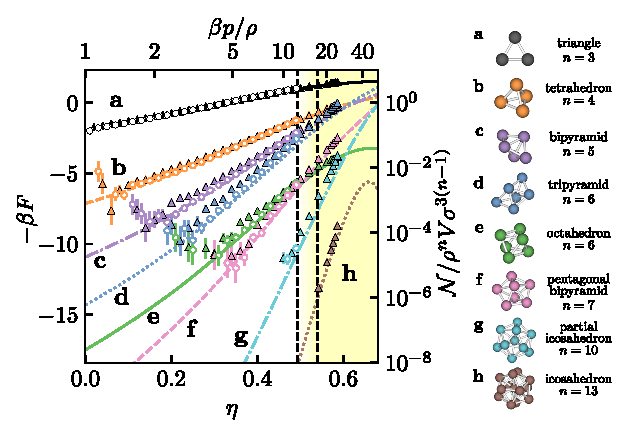
\includegraphics[width=\linewidth,center]{structure-populations}
  \caption[Concentration of local structures in the equilibrium liquid]{
    Static many-body structure in the hard sphere liquid: populations of small local structures in the hard sphere liquid determined from molecular dynamics simulations of 1372 monodisperse (open circles) and 8\% polydisperse (solid triangles) hard spheres against the theoretical prediction of this work (lines).
    Variations against volume fraction $\eta$ and compressibility $Z = \beta p/\rho$ shown.
    The hard sphere freezing and melting volume fractions are indicated by vertical dashed lines.
  }
  \label{fig:structure-populations}
\end{SCfigure}

To demonstrate the effectiveness of this approach we have taken structures for $3 \le n \le 13$ which are global minima of clusters in different simple liquids \cite{Wales2004}.
This set includes frustrated structures for $n \ge 7$ which do not correspond to rigid packings with unique energy minima; we will return to the rigid packings afterwards.
We selected these structures because we can identify them in molecular dynamics simulations using the algorithm of Ref.\ \cite{MalinsTCC2013}.
Using this algorithm we can compare the theoretical predictions against molecular dynamics simulations of both mono- and moderately polydisperse hard spheres at all volume fractions accessed by the simulations i.e.\ $\eta \lesssim 0.585$.
For the polydisperse simulations we used data from Ref.\ \cite{RoyallJSM2017} with a 5-component equimolar distribution with $\sim8\%$ polydispersity, to avoid freezing at high densities, and for the monodisperse simulations we used the DynamO software for event-driven molecular dynamics \cite{BannermanJCC2011}.
We determined their free energies using the thermodynamic integration steps outlined above.

In Fig.\ \ref{fig:structure-populations} we find excellent agreement between the theoretical prediction and the observed concentration of local structure seen in the simulations.
Our approach is able to predict populations of local structures well beyond the regime dynamically accessible to simulation, finding nontrivial structural change deep in the glassy regime highlighted by a rescaling with respect to the trivial $\rho^n$ density contribution.
The free energy of considered structures changes approximately linearly across the entire liquid regime, with deviations from linear becoming more apparent in the supercooled regime.

All structures apart from the fourfold symmetric octahedron in Fig.\ \ref{fig:structure-populations} are subunits of the icosahedron, and increase in concentration more rapidly than the octahedron until high density.
For $n=6$ we consider the free energies of two structures: the tripyramid and octahedron.
We find that the tripyramid occurs $\sim20$ times more often than the octahedron, their free energy difference being dominated by the different point group symmetries following \cite{MalinsJPCM2009,MengS2010}.
We can also estimate vibrational contributions, which allow us to match not only the relative but also the absolute values of free energies obtained from simulation.
In particular, we are able to capture the gradual reduction of the population of octahedral motifs in favour of the tripyramids at high volume fractions.
This is related to the previously observed emergence of fivefold symmetric motifs (such as the full and partial icosahedron) \cite{RoyallPR2015,TarjusJPCM2005,HallettNC2018,DunleavyNC2015}, which is here directly predicted from liquid state theory.

\begin{SCfigure}
  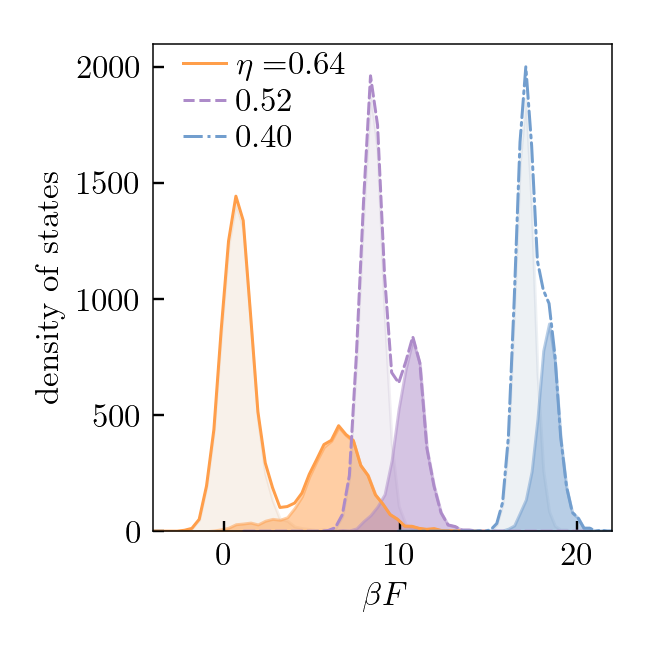
\includegraphics[width=0.9\linewidth,outer]{n12-dos}
  \caption[Free energy distribution of 12 particle structures]{
    Theoretical free energy distribution for the $n=12$ local library of states at several volume fractions.
    The distribution is shifted to lower energies at higher volume fractions, and develops an increasingly bimodal structure.
    Populations are decomposed into those structures containing pentagonal bipyramids without octahedra (light fill) and the remaining structures (dark fill).
  }
  \label{fig:n12-dos}
\end{SCfigure}

Having tested that the theory is accurate for selected geometries, we now take the exhaustive list of 11980 rigid structures for $n=12$ determined in Ref.\ \cite{Holmes-CerfonSR2016} to obtain a local density of states for a given sized inhomogeneity.
We calculated the free energy of all (first-order) rigid structures using \eqref{eq:local-structure-free-energy} (right panel of Fig.\ \ref{fig:structure-populations}), finding a bimodal distribution with two main peaks separated by a free energy difference that increases with increasing volume fraction.
We find the that lower energy distribution consists of structures rich in fivefold (icosahedral) symmetry in the absence of fourfold (octahedral) symmetry.
This shows that the hard sphere liquid is highly frustrated, and would be interpretted as the reason hard spheres make good glassformers in the geometric frustration picture \cite{KivelsonPA1995,TarjusJPCM2005}.
However, this result is potentially compatible with other thermodynamic scenarios like random first-order transition theory (RFOT) \cite{LubchenkoARPC2007}.

Each of the structures correspond to unique contact topologies, but in thermal systems (i.e. with finite gaps between particles) we expect many of them to be indistinguishable as found in Ref.\ \cite{TrombachPRE2018}.
As such, we have likely overestimated the height of the each peak, and especially the lower energy peak which contains more frustrated structures; we will find evidence of this in the next section.
Nevertheless, because this set of packings is exhaustive they represent a complete local density of states in the liquid, which is of fundamental interest to RFOT \cite{LubchenkoARPC2007}.
The distribution of energy levels is a key quantity, but to really examine the connection with dynamics we also need to know the \emph{connectivity} of the different energy states.
For this we need their reaction paths.

We used thermodynamic integration with Monte-Carlo methods to evaluate the free energies in this section, which cannot be straightforwardly applied along reaction paths.
Along reaction paths the geometries are saddles of the potential $\phi^{(n)}$, so the unstable direction must be excluded from integration.
In the next section we introduce analytical methods for evaluating the free energy to address this problem.

%As a Monte-Carlo method it would be very difficult to extend this method to saddles which is of great interest.
%Before moving on to our approximate analytical integration schemes we describe a method which is essentially exact to within numerical precision, at the cost of greater computational expense.

\section{Free energies along reaction paths}
\label{sec:reaction-paths}

While the thermodynamic integration techniques of the previous section are exact in principle, it is desirable to develop analytic approaches for evaluating the free energy.
Analytic approaches are typically faster which is desirable for dealing with larger $n$, as the number of possible packings appears to grow super-exponentially with particle number \cite{Holmes-CerfonSR2016}.
Moreover, analytic approaches are more readily able to calculate free energies along saddles, which are needed to obtain dynamical information in the vein of energy landscape approaches \cite{Wales2004}.

Two methods: assume no hard sphere interactions outside of the bonded particles, or Bayesian inference
\marginfootnote{In the current zeitgeist this could be construed as a form of machine learning; techniques for Bayesian inference are often thrown in with machine learning in e.g.\ topical reviews like Ref.\ \cite{MehtaPR2019}.
  Personally, I am hesitant to call this machine learning as the techniques more closely resemble the approximation schemes of traditional statistical mechanics (to me at least) than neural networks which have been driving the recent machine learning revolution.}

\begin{SCfigure}
  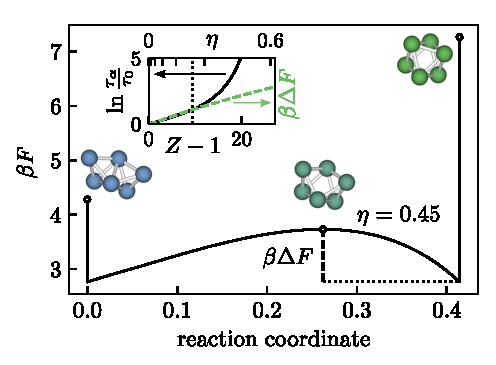
\includegraphics[width=0.9\linewidth,outer]{n6-reaction-path}
  \caption[The simplest nontrivial reaction path in hard spheres: octahedron to tripyramid]{
    Reaction for transition between tripyramid and octahedron $n = 6$ structures.
    Stationary points are indicated by markers: there is a discontinuity in free energy at the end points due to the additional integration over the reaction coordinate, and symmetry in the case of the octahedron.
    Inset: variation of activation barrier with volume fraction $\eta$ and compressibility $Z = \beta p/\rho$ from this theoretical reaction path (dashed line) and measured $\alpha$-relaxation times in bulk molecular dynamics simulations (solid line), where $\eta = 0.45$ is indicated with a vertical dotted line.
  }
  \label{fig:reaction-path-6}
\end{SCfigure}

We have thus far focused on static thermodynamic properties: yet a connection with dynamics can be made by calculating the free energy along reaction paths between (geometrically similar) structures.
This calculation along unstable directions in the free energy landscape requires an analytic approach (described in the SM), and generates paths such as the one in Fig.\ \ref{fig:reaction-path-6}.
Here we consider transitions between the tripyramid and the octahedron with $n=6$ because this is the simplest nontrivial transition between distinct hard sphere packings (SM).
Comparing this dynamical barrier to the structural relaxation for ($\alpha$-) relaxation timescale $\tau_\alpha$ extracted from simulations relative to a microscopic time $\tau_0$ (inset of Fig.\ \ref{fig:reaction-path-6}), we find this single reaction path barrier agrees with the low density scaling of $\tau_\alpha$ (linear in the compressibility factor $\beta p / \rho$ \cite{BerthierPRE2009}).
However, activated dynamics are not expected in this regime so this agreement may be coincidental.
%Moving to high densities, hard spheres exhibit two-step relaxation when vibrational ($\beta$--) and full ($\alpha$--) relaxations decouple as the system approaches its glass transition \cite{Berthier2011}.
%However, dynamics along the tripyramid--octahedron path continues to increase in an ``Arrhenius'' fashion quite unlike the super-Arrhenius increase exhibited by the $\alpha$--relaxation in the computer simulations (inset of Fig.\ \ref{fig:reaction}).
%It has been shown in molecular systems that $\beta$--relaxation can be Arrhenius in the deeply supercooled regime where $\alpha$-- relaxation is super-Arrhenius \cite{Yu2015}.
%Given that typical particle displacements in the tripyramid--octahedron path are around 0.15$\sigma$ per particle, we observe that this relaxation mechanism may be more characteristic of ($\beta$--) relaxation than full ($\alpha$--) relaxation.

\begin{SCfigure}
  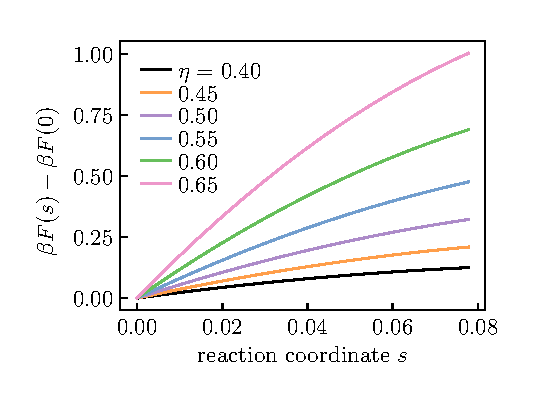
\includegraphics[width=0.9\linewidth,outer]{n7-reaction-path}
  \caption[Reaction path for the two variants of the frustrated pentagonal bipyramid]{
    Reaction for transition between the two $n = 7$ pentagonal bipyramids variant structures, from the variant with a broken spindle (bottom Fig.\ \ref{fig:packings}) to the variant with broken five-fold symmetry (top).
    The free energy increases monotonically along this reaction path, so there is no barrier separating these two structures.
  }
  \label{fig:reaction-path-7}
\end{SCfigure}

It is possible to extend our methodology for larger rearrangements, which may be sufficient to access ($\alpha$-) relaxation \emph{at very deep supercooling} for equilibrium systems.
\todo{Update this with the new Bayesian stuff.}
However, the rapid growth in the number of possible states presents a considerable numerical challenge requiring new methods and approximations, so we leave this exciting avenue for future study.

\section{Conclusions}

We have presented a formalism for describing many-body correlations in liquids and developed it into an accurate and computationally efficient parameter-free theory for hard spheres using integral geometry relying solely on the choice of the equation of state.
The key approximations involved treating the grand potential as continuous and additive (related to extensivity), and imposing the correct contact value of $g^{(2)}(r)$.
\todo{Change this to local structure.}

We applied the framework to a selection of local structural correlations, therefore predicting nontrivial changes in the energy landscape with supercooling putting previous empirical observations on more solid ground.
In particular, our analysis provides evidence for the existence of two populations of structures with distinct symmetries and free energies which causes the local density of states to become increasingly bimodal at high densities.
We note that we have treated densities corresponding to a degree of supercooling only accessible using novel swap Monte Carlo techniques \cite{BerthierPRL2016}; however, these simulations introduce large polydispersity, changing the local structure \cite{CoslovichJPCM2018} and thus limiting direct comparison with our calculations for the monodisperse liquid.

Our framework can be easily adapted to more complex liquids such as systems with soft repulsive interactions and polydisperse mixtures \cite{KodamaJCP2011}.
Integral geometry underlies the core approximation, so this approach can extend to hard particles of more complex shapes where the interaction potential is still geometric in nature.
\todo{Give link to the next chapter!}
It is applicable to a more general class of liquids where the soft part of the potential may be treated as a perturbation around a hard core \cite{Hansen2013} such that a geometric decomposition still applies.
This suggests a new route for predicting static properties of equilibrium liquids, with direct applications to self-assembly, nucleation and protein structure.

%% \section{New notes.}

%% We wish to describe local structure.
%% Ultimately, we wish to learn about the structure of the energy landscape in hard spheres.
%% To do so we must characterise the main features of the landscape, namely the different geometric packings and assign weights (free energies) to them.
%% This is a worthy goal in its own right, perhaps not that interesting for hard spheres but useful for wider applications (e.g.\ predicting self assembly, guiding chemical synthesis, understanding protein folding kinetics and predicting the native state and design).

%% The path we take is as follows:
%% \begin{enumerate}
%% \item We need some means of weighting points in the energy landscape: we do this using the morphometric approach (cf previous chapter)
%% \item A means of characterising and approximating the entire phase space: energy landscape formalism (next). This has two subgoals:
%%   \begin{enumerate}
%%   \item Divide the landscape into stationary points: minima and saddles.
%%     These stationary points characterise submanifolds of the entire landscape, \emph{basins} in the case of minima and \emph{reaction paths} in the case of saddles.
%%   \item Integrate over connected manifolds with weight function (potential of mean force) to obtain their free energies.
%%   \end{enumerate}
%% \end{enumerate}

%% %Another way of saying this is we need an integrand and boundary conditions.

%% \subsection{Connection with energy landscape descriptions}

%% \begin{itemize}
%%   \item First describe the energy landscape description.
%%   \item Based on low-temperature expansion arguments.
%%   \item Mean-field: Laplace method/saddle-point.
%%   \item Gaussian expansion around this result (called Harmonic approximation in energy landscape/chemistry literature).
%% \end{itemize}

%% %% \begin{SCfigure}[H]
%% %%   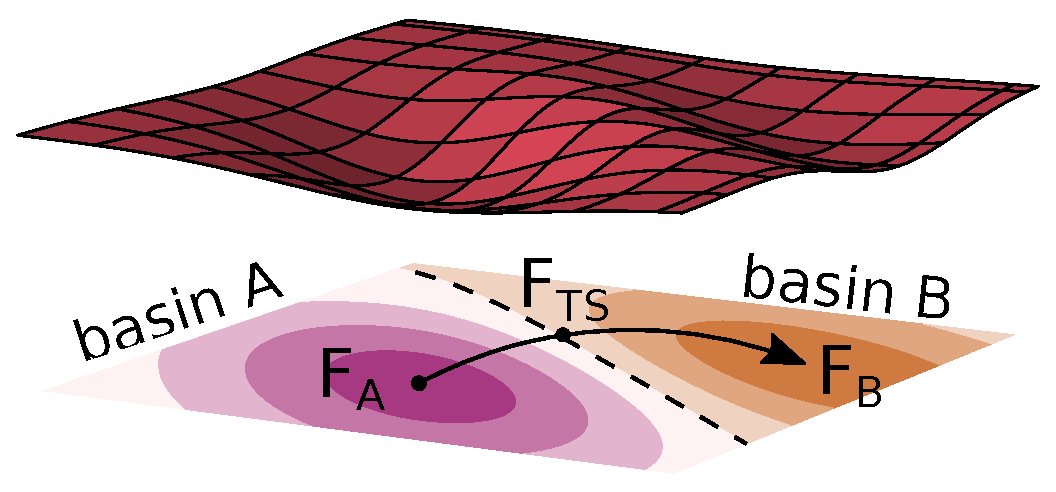
\includegraphics[width=\linewidth,outer]{toy-landscape}
%% %%   \caption[A cartoon energy landscape]{A cartoon energy landscape for a 2-dimensional phase space.
%% %%     The landscape features two local minima: $A$ and $B$.
%% %%     The area surrounding each minima defines its basin: any point from which the minima can be found by moving downhill belongs to the basin.
%% %%     Energy landscape approach: at low temperatures the system is expected to oscillate around potential energy minima, so the dynamics can be understood as rare events causing a change of basin.
%% %%     Thus a decomposition of the phase space in terms of basins should become exact for the dynamics at low temperatures in the supercooled regime of interest.}
%% %% \end{SCfigure}

%% In the case of local arrangements of hard spheres, rigid packings seem to correspond to minima of the potential of mean force.
%% I cannot prove this for the case of morphometric approach, but I cannot find a counter example.
%% Possibly can prove they are minimal volume.

%% \section{Locally favoured structures in hard spheres}

%% \section{Introduction}

%% This study builds on and contributes to work in nonequilibrium statistical physics, particularly relating to glasses and nucleation.
%% Although small-system studies have examined how dynamics are influenced by topographical properties of the energy landscape for simple systems, there has not been a systematic formalism for extending this to the bulk liquid.
%% As such, this study provides additional insight into dynamical arrest i.e.\ the supercooled liquid and glasses.

%% The analytic focus on many-body correlations provides another contribution to the fundamental understanding of simple liquids.
%% This study analyses depletion forces in order to predict the many-body correlation functions in the bulk liquid.
%% Although numerous studies have identified the role of local structure in dynamical arrest little analytical attention has been paid to how to properly formulate structure in a quantitative thermodynamic framework.
%% I address this issue by expressing the solvation free energies in terms of geometrical properties of a small solute, and develop techniques for making quantitative predictions of local structure in the hard sphere liquid.

%% Energy landscape can be divided into two strands: the topographic view of Stillinger which offers a powerful conceptual tool for understanding complex phenomena.
%% At low temperatures we can imagine the system oscillating around low energy minima (inherent states), with occasional large fluctuations driving it through `choke points' causing a change to a different energy minimum.
%% This formalism was turned into a properly quantitative framework by Wales \cite{Wales2004,?}, where stationary point databases are constructed: energy minima connected by saddles.
%% From the connectivity of the landscape one can understand dynamical arrest: if there are lots of competing low lying minima it can be hard for the system to find the global minimum and we expect it to fall out of equilibrium easily when temperature is lowered.
%% By contrast, if the minima steadily lower in energy then they act as a funnel to the global minimum so we expect rapid equilibration.

%% Quantitative predictions are typically only possible for small systems, so it is desirable to extend it to the bulk.
%% One can to do this focusing on a subset of the total degrees of freedom, integrating out the rest in an approximate fashion.
%% The selected degrees of freedom act as a small system with a many-body interaction potential, so can be treated with the aforementioned formalism in a quantitative manner.
%% This was attempted by Tarjus \cite{?} with mixed success.
%% The morphometric approach \cite{KonigPRL2004,RothPRL2006,RobinsonPRL2019} offers a generic framework to treat many-body correlations allowing a first-principles treatment of local structure in the bulk liquid.
%% This framework is accurate for hard spheres where it has been extensively tested \cite{Hansen-Goos?,Roth?,Bob?,RobinsonPRL2019}.

%% Hard particle systems are the fundamental system of interest for simple liquids.
%% The stationary point database approach, firmly rooted in \emph{potential energy}, fails for hard systems as the potential energy is trivial so the thermodynamics is athermal.
%% It has never been extended to hard systems until now.
%% This extension comes with the cost that some of the elegant techniques of soft systems will fail due to the singular nature of hard sphere interactions, so we require new methods to handle the idiosyncrasies of hard systems.
%% Here we propose a practical definition for basins when working with hard systems, and develop techniques for evaluating thermodynamic quantities with this definition.
%% We then retroactively justify the meaningfulness of this basins by comparing with simulation/literature data.

%% \todo{Talk about the past work on hard spheres: penny packing, and sticky spheres.}
%% A number of unique technical challenges brought about by the hard sphere potential, that we will solve.
%% The groundwork for this was laid down by Holmes-Cerfon and coworkers.
%% Note: attempts have been successful at modelling effective interactions close to isostaticity where $z \to 2d$.
%% This is empirically found to be the case asymptotically as one approaches jamming, however it is worth noting that there is no general requirement that $z = 2d$ for rigid packings, and counter examples where $z < 2d$ are known.

%% In section \ref{sec:energy-landscapes} we review the energy landscape formalism for soft potentials, with a view to highlighting where it might fail for hard interactions.
%% We review the liquid state theory/morphological approach used for treating the depletion interactions between hard particles in the bulk liquid in section \ref{?},
%% followed by the equivalent of the partition function for local structure.
%% Our core theoertical results are then presented in section \ref{?}, where we propose a definition of local structure and show techniques for evaluating the partition function nonperturbatively.
%% We then present the results of the topography of the local structural energy landscape in hard spheres in section \ref{?}, our main numerical results.

%% \section{Energy landscape approaches}
%% \label{sec:energy-landscapes}

%% Points to cover:
%% \begin{itemize}
%% \item Give a technical definition of local structure with a goal to showing the problems with hard systems.
%% \item Define structures as manifold: $\mathbb{R}^{dn}$ for $n \ll N$, embedded in $\mathbb{R}^{dN}$
%% \item Failure of perturbation theory due to singularity of
%% \end{itemize}

%% The energy landscape/inherent structure approach is a powerful theoretical framework for understanding complex phenomena.
%% At its core, it is a means of coarse-graining the high dimensional phase space into a more manageable mesostates.
%% Its power comes from the fact that it is essentially exact, though calculations are typically intractable unless the degrees of freedom can be significantly reduced; in practice this is generally only possible in mean field (high spatial dimensions) or for small systems $N = \mathcal{O}(10)$ in physical settings.
%% The approach is however useful conceptually for developing theories based around the topography of the energy landscape \cite{Stillinger}, and makes detailed calculations tractable typically for small systems \cite{Wales2004}.

%% In this section we will review the energy landscape approach, how it applies to soft potentials and the complications that arise for our system of interest: hard spheres.
%% First we talk about coarse-graining into mesostates mentioned above, whether into inherent structures or otherwise.
%% A mesostate is a collection of microstates which are grouped together, typically these are selected for sharing some desirable property to simplify description.
%% For practical reasons this means that microstates should be connected in phase space so they are compact manifolds.
%% In connection with the topographic view we will call these manifolds \emph{basins}.
%% The total partition function is then decomposed as
%% \begin{equation}
%%   Z \equiv \int_{\mathbb{R}^{dN}} e^{-\beta (U_N(\vec{r}^n) + \phi(\vec{r}^n))} \, d\vec{r}^N = \sum_i Z_i
%% \end{equation}
%% where $\phi$ is the external potential of the container in order to keep the particles localised in a region where they interact.
%% Alternatively they could be embedded in a toroidal topology to prevent particle dissociation (as in e.g.\ simulations with periodic boundary conditions).
%% The basin partition function is
%% \begin{equation}
%%   Z_i = \int_{\mathbb{V}_i^{dN}} e^{-\beta U_N(\vec{r}^N)} \, d\vec{r}^N
%% \end{equation}
%% if $\mathbb{V}_i^{dN} \subset \mathbb{R}^{dN}$ is the manifold corresponding to basin $i$.
%% One can define (e.g.\ Wales).
%% Despite a definition which unambiguously demarcates the basins, the high dimensionality of the phase space renders the integrals in \eqref{eq:basin-partition-function} completely intractable without approximation.

%% The equilbrium probability of the system being in basin $i$ at any one time is thus
%% \begin{equation}
%%   p_i = \frac{Z_i}{Z}
%% \end{equation}
%% From the Gibbs-Shannon entropy we find the coarse-graining entropy
%% \begin{equation}
%%   \begin{split}
%%     S_{\textrm{conf}}
%%     &= -\sum_i p_i \ln{p_i} \\
%%     &= -\sum_i \left( \frac{Z_i}{Z} \ln{Z_i} - \frac{Z_i}{Z} \ln{Z} \right) \\
%%     &= \ln{Z} - \sum_i \frac{Z_i}{Z} \ln{Z_i}
%%   \end{split}
%% \end{equation}
%% Noting that the total free energy is $F = -k_B T \ln{Z}$ we thus have
%% \begin{equation}
%%   \beta F = \langle \beta F_i \rangle - S_{\textrm{conf}}
%% \end{equation}
%% where the average basin free energy $F_i = -k_B T \ln{Z_i}$ is
%% \begin{equation}
%%   \langle \beta F_i \rangle = - \frac{1}{Z} \sum_i Z_i \ln{Z_i}
%% \end{equation}

%% Finally, we have to choose how to define the basins.
%% In the energy landscape approach the coarse-graining occurs around local minima of energy where $\vec{\nabla}U_N = 0$ and Hessian $\frac{1}{2}\vec{\nabla}\vec{\nabla}U_N$ is positive definite.
%% Each basin consists of all the points connected by a steepest descent path to a unique energy minimum.
%% This description reduces the high dimensional continuous description down to discrete number of zero-dimensional manifolds.
%% In practice the number of minima scales exponentially in $N$, so this is still an intractably large number of points.
%% One can even obtain dynamical information by considering the saddles, i.e.\ the unstable stationary points.
%% The saddles act as the lowest (in energy) lying points that must be crossed to jump from one basin to another, giving the energy barriers to dynamics.

%% How do we justify this approach?
%% Energy is smooth so asymptotics around stationary points is valid: inherent state (stable stationary points) description
%% For infinite systems we could use Laplace method
%% \begin{equation}
%%   \int_{\mathbb{V}^{dN}_i} e^{-\beta N u_N(\vec{r}^N)} \, d\vec{r}^N
%%   \sim
%%   e^{-\beta \min{U_N(\vec{r}^N)}} \qquad \forall \; N \gg 1
%% \end{equation}
%% where $u_N = U_N / N$.
%% For finite systems we could go beyond this pertubatively by employing a harmonic approximation from the energy-landscape literature
%% \begin{equation}
%%   U_N = U_N(\vec{p}_i) +
%%   \frac{1}{2} \Delta \vec{r} \cdot \left. \nabla \nabla U_N\right|_{\vec{p}_i} \cdot \Delta \vec{r}
%%   + \mathcal{O}(\Delta \vec{r}^3)
%% \end{equation}
%% where \[\vec{p}_i = \argmin_{\vec{r}^n \in \mathbb{V}_i^{dN}}{\left(U_N(\vec{r}^n)\right)}\] is the location of the energy minimum.
%% \begin{equation}
%%   Z_i \sim \exp{-\beta U_N(\vec{p}_i)}
%% \end{equation}
%% There are two layers of approximation: first we model the pdf as a Gaussian, second we approximate the boundary conditions as being infinite.
%% The inclusion of the Hessian term in the expansion around the minimum shows that for soft potentials one can perturbatively build a description around the inherent states.
%% At low temperatures this approach is expected to become exact (for the first layer not the second one).
%% So for athermal systems perturbation theory should break down.

%% \begin{SCfigure}
%%   \missingfigure[figwidth=\linewidth]{}
%%   \caption{Failure of Laplace method for hard interactions.}
%% \end{SCfigure}

%% To make the above discussion concrete we will consider two examples.
%% First, we examine a symmetric quartic potential
%% \begin{equation}
%%   \phi = \epsilon (x^4 - x^2)
%% \end{equation}
%% where $x$ is some state variable and $\epsilon$ is an energy scale.
%% This could represent e.g.\ a ferromagnet below the critical temperature with $x$ representing the spontaneous magnetisation.
%% The free energy in units of $\epsilon$ is then
%% \begin{equation}
%%   F = - T \ln{\left( \int \exp{\left(-\frac{\phi}{T}\right)} \, dx \right)}
%% \end{equation}
%% This potential naturally contains two basins for the two half space $x \in [-\infty, 0]$ and $x \in [0, \infty]$, and because of the symmetry of the potential around $x=0$ the contribution of each of these basins is identical, i.e.\
%% \begin{equation}
%%   Z = 2 \int_0^\infty \exp{\left(-\frac{\phi}{T}\right)} \, dx.
%% \end{equation}
%% Applying the harmonic approximation
%% \begin{equation}
%%   \begin{split}
%%   Z &\simeq
%%   2 \exp{\left( -\frac{\phi(x_0)}{T} \right)}
%%   \int_{-\infty}^\infty \exp{\left(-\frac{\phi''(x_0)}{2T}\right)} \, dx \\
%%   &=
%%   2 \exp{\left( -\frac{\phi(x_0)}{T} \right)}
%%   \sqrt{\frac{2 \pi T}{\phi''(x_0)}}
%%   %+ \mathcal{O}(\phi'''(x_0))
%%   \end{split}
%% \end{equation}
%% where $x_0 = \dfrac{1}{\sqrt{2}}$ is the position of the minimum in the $x > 0$ basin.

%% To summarise this section, we note that the basin definition of structures for soft potentials has the properties that: \cite{Wales?}
%% \begin{itemize}
%% \item Each basin $B_i$ connects to a unique minimal energy state with a unique geometry.
%% \item Divide the phase space into basins which do not overlap $B_i \cap B_j = \emptyset$ for $i \ne j$ and tile the whole of phase space $\cup_i B_i = \mathbb{R}^q$.
%% \item Its free energy is well-defined (at least in some asymptotic limit) so it can be approximated with simple methods.
%%   For soft potentials this is a consequence of the first criterion.
%%   This makes the choice of coarse-graining (thermo)dynamically meaningful: it is long-lived enough that the microstates making up a basin can be not distinguished, and the dynamics reduces to basin crossing events.
%% \end{itemize}
%% A definition satisfying the first two criteria is possible, however due to the singularity in the hard particle interaction potential the region surrounding the (depletion) energy minimum is thermodynamically irrelevant.
%% This can be interpretted:
%% \begin{itemize}
%% \item \emph{Thermodynamically}: the region near contact is entropically suppressed, regions away from contact have many more microstates so are entropically enhanced
%% \item \emph{Dynamically}: as hard spheres approach one another they collide and bounce away so spend infinitesimally small timescales at contact.
%%   Collisions almost universally involve only two particles, collisions of more than two particles occur with zero measure.
%% \end{itemize}
%% Because of this we cannot obtain the free energy by a small parameter expansion around the contact point.
%% We must evaluate the full integral over a finite volume.
%% To make this tractable we will abandon the rigorous definition of structures in terms of basins employed for soft potentials, in favour of a simple one based on intuitive geometrical ideas.
%% We will later explore the limitations/successes of this definition in order to retroactively justify this approach.

%% Due to the analogies between the population/concentration integral and the usual partition function, we will refer to this integral simply as a partition function.

%% \subsection{Molecular partition function}

%% From the definition of the probability density function in Eq.\ \eqref{eq:n-density-pdf}, the total number of local structures of a particular type in a volume $V$ is
%% \begin{equation}\label{eq:structure-population}
%%   \mathcal{N} =
%%   \int_{\mathcal{Q}} \rho^n g^{(n)}(\vec{r}^n) \, d\vec{r}^n,
%% \end{equation}
%% where $\mathcal{Q}$ is the domain \emph{defining} the local structure.
%% To get the free energy expression used in the main text we consider the manifold diffeomorphic to translations, defining $\mathcal{Q} = \mathcal{D} \rtimes \mathbb{V}$ where $\mathbb{V}\subset \mathbb{R}^3$ is the system volume.
%% Exploiting translational invariance of the potential of mean force, we fix one particle at the origin and integrate the center of mass over the system volume giving
%% \begin{equation}
%%   \mathcal{N} =
%%   \rho^n V \int_{\mathcal{D}} g^{(n)}(\vec{r}^n) \, d\vec{r}^{n-1}.
%% \end{equation}
%% We defined a free energy by taking $\mathcal{N} = \sigma^{3(n-1)} \rho^n V e^{-\beta F}$, which together with the above expression gives Eq.\ \eqref{eq:local-structure-free-energy} in the main text.

%% There will be $d$ translation modes and $\frac{d(d-1)}{2}$ rotational modes for each plane formed by pairs of coordinate axes (e.g.\ $x^1 \wedge x^2$ for rotations in the $x^1x^2$-plane).
%% Subtracting the number of rigid body modes from the total degrees of freedom gives \[ q = dn - \frac{d(d+1)}{2} \] internal degrees of freedom.
%% Exception when rotations are degenerate: $n < d$ (e.g.\ $n=2$ in $d=3$) or pathological cases of unusually high symmetry (e.g.\ when all particles fall on a line) which can in general be excluded.

%% More generally, we consider the manifold diffeomorphic to translations \emph{and} rotations.
%% We define $\mathcal{Q} = \mathcal{D}' \rtimes SE(3)$ where $\textrm{SE}(d)$ is the $d$-dimensional special Euclidean group, leaving the $\mathcal{D}'$ as the space of the structure's internal motion.
%% We separate rigid body from internal motion by applying the following transformation to each particle coordinate
%% \begin{equation}
%%   \vec{r}(\{\vec{t}, \vec{\theta}, \vec{x}\}) =
%%   \vec{t} + \vec{R}(\vec{\theta}) \cdot \vec{q}(\vec{x}),
%% \end{equation}
%% where $\vec{t}$ is the translation vector, $\vec{\theta}$ the Euler angles, $\vec{R}$ the rotation matrix, and $\vec{x} \in \mathbb{R}^{3n-6}$ represents the internal coordinates.
%% We need to compute the metric of this transformation $G_{ij} = \vec{G}_i \vec{G}_i^T$ where the (generally curvilinear) basis vectors are $\vec{G}_i = \partial_i \vec{r}$.
%% To simplify calculation we choose $\vec{q}(\vec{x})$ to always be in the center-of-mass frame and orthogonal to rotations such that $G_{ij}$ reduces to block-diagonal form.
%% If the rotation matrix is expressed in Euler-angle representation as $\vec{R}(\vec{\theta}) = \vec{R}_3(\theta_3) \vec{R}_2(\theta_2) \vec{R}_1(\theta_1)$ then we have%
%% \footnote{While the final form of $\vec{G}$ is elegant, I do not have a straightforward way of getting it; it involved a lot of guesswork and within Mathematica to find a form of $\vec{U}$ which gives the middle block.
%%   There is probably a more direct route.}
%% \begin{equation}
%%   G_{ij}(\{\theta_i\}, \vec{x}) =
%%   \begin{pmatrix}
%%     n \vec{E} & 0 & 0 \\
%%     0 & \vec{U}^T(\vec{\theta}) \vec{M}(\vec{x}) \vec{U}(\vec{\theta}) & 0 \\
%%     0 & 0 & \overline{G_{ij}}(\vec{x})
%%   \end{pmatrix},
%% \end{equation}
%% where $\vec{E}$ is the identity matrix, $\vec{M}$ is the moment of inertia tensor, $\overline{G_{ij}}$ is the metric for internal motion, and we have defined the matrix $\vec{U}$ as
%% \begin{equation}
%%   \vec{U}(\vec{\theta}) =
%%   \begin{pmatrix}
%%     1 &  0              & -\sin{\theta_2} \\
%%     0 &  \cos{\theta_1} &  \cos{\theta_2} \sin{\theta_1} \\
%%     0 & -\sin{\theta_1} &  \cos{\theta_2} \cos{\theta_1} \\
%%   \end{pmatrix}
%%   \qquad
%%   \begin{aligned}
%%     \theta_1 &\in [0,2\pi] \\
%%     \theta_2 &\in \left[-\frac{\pi}{2},\frac{\pi}{2}\right] \\
%%     \theta_3 &\in [0,2\pi].
%%   \end{aligned}
%% \end{equation}
%% Note $\det{\vec{U}} = \cos{\theta_2}$.
%% The volume element in the new coordinates is
%% \begin{equation}
%%   d\vec{r}^n = \frac{\sqrt{\det G_{ij}(\vec{x})}}{\nu}
%%   \, d^3 \vec{t} \, d^3 \vec{\theta} \, d^{3n-6} \vec{x},
%% \end{equation}
%% where $\nu$ is the symmetry number (discussed below) and
%% \begin{equation}
%%   \sqrt{\det G_{ij}(\vec{x})} =
%%   \cos{\theta_2} \sqrt{\det{\vec{M}(\vec{x})}}
%%   \sqrt{n^3 \det{\overline{G_{ij}}(\vec{x})}}.
%% \end{equation}
%% The symmetry number emerges as the choice of internal coordinates typically fixes the particle labels breaking permutation symmetry; we have to multiply by the $n!$ possible labellings, which introduces double counting if the structure possesses rotational symmetry so we have to divide by the correcting factor $\nu$.
%% This is explained in detail in Ref.\ \cite{CatesSM2015}.
%% Thus \eqref{eq:structure-population} reduces to
%% \begin{equation}\label{eq:structural-partition-function-detailed}
%%   \frac{\mathcal{N}}{\rho^n V}
%%   =
%%   \frac{8\pi^2 \sqrt{n^3}}{\nu} \int_{D'}
%%   g^{(n)}(\vec{x}) \,
%%   \sqrt{\det{\overline{G_{ij}}(\vec{x})} \det{\vec{M}(\vec{x})}}
%%   \, d^{3n-6} \vec{x}.
%% \end{equation}
%% Note that in the limit of linear molecules, i.e.\ where all particles fall on a line, the above approach fails as there is one less rotation mode requiring a modified description.

%% Note that for all of the geometries we have tested this metric seems to be 2, although we could not prove this is in the general case.
%% We have to actually evaluate the integral.
%% We will explore thermodynamic integration using Monte Carlo, which is essentially exact to numerical precision but slow, and some analytical approximations.

%% \subsection{Worked examples}

%% %% \begin{SCfigure}
%% %%   \missingfigure[figwidth=\linewidth]{}
%% %%   \caption{Number of first shell neighbours in the hard sphere liquid.}
%% %% \end{SCfigure}

%% %% \begin{SCfigure}
%% %%   \missingfigure[figwidth=\linewidth]{}
%% %%   \caption{Number of equilateral triangles in the hard sphere liquid.}
%% %% \end{SCfigure}

%% We will consider two worked examples for simple geometries which are readily visualised and for which the metric $G(\vec{x})$ is known exactly and the partition function integral reduces to a simple form.

%% Our first worked example is at the two-body level: the typical number of neighbours in the first shell.
%% For a dimer the metric term evaluates to $G(\vec{x}) = r^2$, i.e.\ the usual spherical coordinate Jacobian as expected.
%% The average number neighbours less than some distance $r$ is then
%% \begin{equation}
%%   z(r)
%%   = 4\pi \int_0^r g^{(2)}(r) r^2 \, dr
%%   = 4\pi \int_\sigma^r e^{-\beta \phi^{(2)}(r)} r^2 \, dr
%% \end{equation}
%% This is a common measurement where $r$ is taken up to the first minimum of the $g(r)$ then $z$ corresponds to the number in the ``first-shell'' (i.e. the coordination number).

%% Our second worked example considers the average concentration of triangles in the liquid.
%% Here the relevant coordinates are the tuple $\vec{x} = (r,s,t)$ where the three distances are the lengths of the triangle.
%% The metric has previously been determined exactly as $G(\vec{x}) = rst$ in \cite{?}.
%% The number of equilateral triangles with maximum side length $\delta$ is then
%% \begin{equation}
%%   N_\Delta(\delta)
%%   =
%%   8\pi^2 \int_\sigma^\delta\int_\sigma^\delta\int_\sigma^\delta
%%   e^{-\beta\phi^{(3)}(r,s,t)} rst \, dr ds dt.
%% \end{equation}
%% The results show excellent agreement with molecular dynamics simulations across the entire liquid regime, and even into the supercooled regime where simulations are available for a polydisperse system.

%% \section{Results}

%% We take the minimal energy structures as the stable packings determined in Refs.\ \cite{ArkusPRL2009,Holmes-CerfonSR2016}.
%% For each landscape with $n \le 5$ there is only a single stable packing, i.e.\
%% \begin{itemize}
%% \item Dimer $n=2$
%% \item Equilateral triangle $n=3$
%% \item Tetrahedron $n=4$
%% \item (Triangular) bipyramid $n=5$
%% \end{itemize}
%% However for $n = 6$ we first see two competing packings: the tritetrahedron and the octahedron.

%% At $n = 7$ there are 5 stable packings, including two subgraphs of the pentagonal bipyramid each with a broken bond: one has a broken spindle, the other a broken ring.
%% This is a well known property of hard sphere packings, and the cause of geometric frustration: it is generally well-established \cite{?,?,?,Robinson?} that 5-fold symmetric structures are lower in (free) energy for simple systems, however they do not tile space perfectly leading to the suppresion of long-range ordering.
%% For soft systems this frustration can be overcome and all of these `contraints' can be satisfied \cite{Frank,Wales}.
%% However, if we look at the one-dimensioinal reaction paths for n=7 we see that there is not thermal barrier separating these two structures.
%% This shows that they should not be distinguished in the liquid regime, showing the limitation of our definition of structure: they are simply thermal fluctuations of one another.
%% We have overcounted the number of stable structures for $n=7$ by one.
%% For similar reasons we have likely overestimated number of structures in n = 12 landscape, but does not change the fact that they are lower in energy

%% Comparing accuracy of analytical integration methods, we find a systematic error increasing with volume fraction likely due to the perturbation in the potential of mean force.
%% For most of the structures the error scales with a similar magnitude and the same sign (see Fig.\ \ref{?}), suggesting a systematic error.
%% Numerical experiments for $g^{(3)}$ show that the main source of error is the order of the expansion, with second-order significantly improving it and third-order being essentially exact.
%% We cannot distinguish the result with the true metric from the that with the approximate metric: this is not a big source of error, at least not for $n=3$ where we can test it.

%% However for a subset of the structures we find that the error has the opposite sign, due to a different source of error: the neglect of additional hard sphere interactions.
%% \todo{Collapse all the data onto a single figure.
%%   Can we rescale the error by the free energy?
%%   What can we correlate?}
%% Using expectation propagation the sign of the error is restored showing that we are treating these interactions, though the error is generally larger than for the other structures as it is not an exact method.
%% \todo{Can we include the potential expansion to second order?}

%% \begin{SCtable}
%%   \begin{minipage}[b]{\linewidth}
%%     \centering
%%     \begin{tabular}{cccc}
%%       Structure & $\beta F(\eta=0.45)$ & $\beta F(\eta=0.56)$ & $\beta F(\eta=0.64)$ \\
%%       \hline
%%       1 & 0.5 & 0.7 & 0.9 \\
%%       2 & 0.5 & 0.7 & 0.9 \\
%%       3 & 0.5 & 0.7 & 0.9 \\
%%       4 & 0.5 & 0.7 & 0.9 \\
%%       5 & 0.5 & 0.7 & 0.9 \\
%%     \end{tabular}
%%   \end{minipage}
%%   \caption{Free energies of structures for $n=7$ landscape at varying volume fractions.}
%% \end{SCtable}

%% \begin{SCfigure}
%%   \missingfigure[figwidth=\linewidth]{}
%%   \caption{Distribution of energy levels for $n \le 9$.
%%   Include saddles.}
%% \end{SCfigure}

%% \begin{SCfigure}
%%   \missingfigure[figwidth=\linewidth]{}
%%   \caption{Distribution of energy levels for $10 \le n \le 12$.}
%% \end{SCfigure}

%% Next we give the minimal energy structures for $8 \le n \le 12$.

%% \section{Discussion}

%% Here we summarise our many layers of approximations.
%% First, we have to make a \emph{choice} over how to coarse-grain the phase space.
%% This is not strictly an approximation, but it defines what we mean by a `structure' and informs the approximations used to compute the free energies.
%% Then, we make the following approximations:
%% \begin{enumerate}
%% \item Morphological approach for correlations:
%%   \begin{enumerate}
%%   \item Morphometric \emph{ansatz}
%%   \item Virial choice of closure with Carnahan-Starling equation of state
%%   \end{enumerate}
%% \item Expansions of geometrical measures:
%%   \begin{enumerate}
%%   \item Second-order expansion of geometric measure (i.e.\ moment of inertia)
%%   \item Contact measure for bond-distance space (i.e.\ zeroth-order term): this seems to be more or less exact for $n=3$
%%   \end{enumerate}
%% \item First-order expansion of potential around contact (can we get second?)
%% \item Polyhedral approximation of boundary conditions (additional hard sphere bonds).
%% \item Bayesian inference to perform integral
%% \end{enumerate}
%% \todo{Mention how we nudge the coordinates with a small perturbation from the contact point to prevent problems with e.g.\ four-particle intersections (and higher)}

%% We found that two 5-fold symmetric structures at $n=7$, both pentagonal bipyramids with broken symmetries, are not separated by a thermodynamic barrier.
%% This means they should be considered as thermal fluctuations of one another, and not be distinguished.
%% This explains why 5-fold symmetric structures like the icosahedron are thermally stable in the hard sphere liquid.
%% Note that at jamming the symmetry of these structures must be broken.

\ifdefined\includebibliography
  \newgeometry{margin=1in}
  \printbibliography
\fi

\end{document}

%TC: macro \marginfootnote [other]
%TC: envir SCfigure [] other
%TC: macrocount beginSCfigure [figure]
\documentclass[11pt,twoside]{report}
\usepackage{preamble}
\setcounter{chapter}{4}
\graphicspath{{../img/}}
\def\includebibliography{}

\externaldocument{background}

\begin{document}
\chapter{Morphological thermodynamics for hard bodies from a controlled expansion}
\epigraph{He said that the geometry of the dream-place he saw was abnormal, non-Euclidean, and loathsomely redolent of spheres and dimensions apart from ours.}{H.\ P.\ Lovecraft, \emph{The Call of Cthulhu} (1926).}
\label{chapter:resummation}

\section{Introduction}

The standard theoretical framework for treating inhomogeneous liquids is classical density functional theory (DFT).
Central to this theory is the result that the free energy can be \emph{exactly} expressed as a functional of the density $\Omega = \Omega[\rho(\vec{r})]$ \cite{EvansAP1979}, though approximate functionals must be used in general.
For example, the fundamental measure theory (FMT) \cite{RosenfeldPRL1989} provides a class of highly accurate functionals for the hard sphere liquid.
% relying on physical ingenuity.
A common practical application of DFT is to its \emph{dual} problem: determining the free energy $\Omega = \Omega[\phi_\mathrm{ext}(\vec{r})]$ for a fixed external potential $\phi_\mathrm{ext}(\vec{r})$.
Approaching this through DFT requires minimisation of $\Omega$ to obtain the equilibrium density profile, a tractable but expensive procedure.
In situations where many function evaluations are required, e.g.\ when integrating over many different realisations of $\phi_\mathrm{ext}$, this minimisation operation can become prohibitively expensive.
It is worthwhile to investigate more direct routes to approximating $\Omega[\phi_\mathrm{ext}(\vec{r})]$, especially where accuracy may be less important than fast calculation.

A promising approach to the dual problem is through morphological thermodynamics \cite{KonigPRL2004} with the potential to enable fast and accurate calculations in hard spheres \cite{RothPRL2006,Hansen-GoosPRL2007,RobinsonPRL2019}.
The morphometric approach concerns sharply repulsive external potentials where $\phi_\mathrm{ext}$ acts as a container for the fluid or as an exclusion volume for e.g.\ a solute.
In this limit the density profile is negligible over a volume $V$, and the free energy is expanded in terms involving $V$ and its boundary $\partial V$.
In this approximation the free energy change from its homogeneous value $\Delta \Omega := \Omega[\phi_\mathrm{ext}] - \Omega_\mathrm{hom}$ is expanded as
\begin{equation}\label{eq:morphometric-approach}
  %\Omega[\phi_\mathrm{ext}] - \Omega_\mathrm{hom}
  \Delta \Omega
  =
  p V + a_2 A + a_1 C + a_0 X,
\end{equation}
where $p$ is the pressure and $\{a_2,a_1,a_0\}$ are coefficients for the surface terms $A$, the area; $C$, the integrated mean curvature; and $X$, the integrated Gaussian curvature.
The surface terms are normally determined from the integrals
\begin{subequations}
  \begin{align}
    A &= \int_{\partial V} \, dA \\
    C &= \frac{1}{2} \int \Tr{\kappa} \, dA \\
    X &= \int_{\partial K} \det{\kappa} \, dA
  \end{align}
\end{subequations}
where $\kappa$ is the curvature tensor on the surface.

Despite its accuracy in hard spheres the morphometric expansion \eqref{eq:morphometric-approach} is still an approximation, as numerous detailed investigations have shown \cite{OettelEL2009,AshtonPRE2011,LairdPRE2012,BlokhuisPRE2013,UrrutiaPRE2014,Hansen-GoosJCP2014}.
Fundamental questions remain over \emph{why} it is accurate and how one might improve the approximation.
Inaccuracies become significant in hard spheres at very high densities approaching the glass transition \cite{RobinsonPRL2019,RobinsonPRE2019}, so an approximation scheme including additional terms could be desirable for approaches to dynamical arrest.
An important feature of the geometric terms in the morphometric approach is that they remain well defined even where a curvature tensor is not locally definable, at e.g.\ a cusp; this property is central to the success of the expansion \eqref{eq:morphometric-approach} so that the coefficients can be independent of the geometry.
Correspondingly, proposed approximations of $\Omega[\phi_\mathrm{ext}(\vec{r})]$ which do not share this feature can be ruled out as general expansions.

To illustrate this we consider what happens if one attempts to extend \eqref{eq:morphometric-approach} by including higher moments of curvature.
A prototypical example of this is the \emph{Helfrich expansion} for elastic membranes \cite{HelfrichZFNC1973}, which is often argued to be the most general expansion for the surface tension.
The next highest order term to augment \eqref{eq:morphometric-approach} would be
\begin{equation*}
  \int_{\partial V} \left(\Tr{\kappa}\right)^2 dA,
\end{equation*}
which is not well-defined for general surfaces, in particular for surfaces containing vertices and/or arcs as occurs in e.g.\ polyhedra.
To demonstrate this we consider the line where two planes intersect with dihedral angle $\Delta \theta$.
This can be considered as a cylindrical sector in the limit of vanishing radius $r$, giving the contribution per unit length
\begin{equation*}
  \int \left(\Tr{\kappa}\right)^2 r d\theta
  = \frac{\Delta \theta}{r}
\end{equation*}
diverging as $1 / r$ in the limit where the sector becomes an arc $r \to 0$.
We find that only the curvature terms already present in the morphometric approach are well-defined in general, so coefficients of any additional curvature moments must necessarily be zero within a controlled expansion.
The inclusion of higher-order curvatures was originally motivated by continuum elasticity \cite{HelfrichZFNC1973}, so it is not surprising that features on small lengthscales are pathological.
In this work we will attempt to start the path towards supplementing the morphometric approach \eqref{eq:morphometric-approach} with higher-order terms, by deriving the known terms as the leading contribution in the only properly rigorous free energy expansion: the \emph{virial series}.

%% Our argument can be summarised by.
%% This is not a surprising fact in itself as the morphometric approach can be obtained as a limit case of FMT \cite{Hansen-GoosJPCM2006}.
%% Our central argument is that the strength of the morphometric approach comes from underlying agreement with the leading contributions in the (exact) virial expansion, so a proper extension should be rooted in the virial series.
%% Homogeneous is simpler, so extensions may be possible where they are not in the inhomogeneous case.

%% To do this we will explore how this approach emerges from the virial expansion and what form it takes for other shapes and mixtures.
%% The virial expansion provides a few exact results which can be used to explore the limitations of approximate theories.

In sections~\ref{sec:low-densities} and \ref{sec:hard-rods} we will present the limiting cases where the insertion cost rigorously takes the morphometric form, i.e.\ the low density limit and for one-dimensional hard rods.
In section~\ref{sec:finite-densities} we resum the terms contributing in these exact limits to obtain a piece of the solvation energy which \emph{exactly} obeys the morphometric form, and we are able to calculate the thermodynamic coefficients explicitly.
Our main result is valid for hard interactions where the solute and solvent particles are convex.
Though applicable to arbitrary mixtures of particle geometries, the resulting form is equivalent to the standard morphometric approach \eqref{eq:morphometric-approach}.
The methods we use are identical to those used in analysis of inhomogeneous FMT, reflecting the deep underlying connections between FMT and the morphometric approach \cite{LeithallPRE2011,KordenPRE2012,MarechalPRE2014}.

%% The motivation for doing this is primarily to justify the morphometric approach by demonstrating that additional contributions are small for hard spheres, and from this develop an understanding of where the approach may fail.
%% The analytical thermodynamic coefficients we obtain provide a starting point for modelling new systems where a theory may not be available.
%% Furthermore, we use the form of the exact contribution to argue that the generalisation to mixtures suggested in \eqref{eq:morphometric-approach-mixtures} is unnecessary, as the exact contribution has the simpler form of \eqref{eq:morphometric-approach}.
%% Finally, the framework we use to obtain this contribution is \emph{identical} to the virial expansion approach for FMT; this approach has been systematically explored in the more general case of inhomogeneous systems \cite{LeithallPRE2011,KordenPRE2012,MarechalPRE2014}.
%% By applying this approach to our much simpler (essentially homogeneous) system we hope to make the ideas and techniques more accessible.

%% Historically, the morphometric approach has been argued on the grounds laid out above, and as a limiting case of FMT.
%% The goal in subsequent sections will be to review the many arguments to understand why it works, reveal its limitations and inform better approximation schemes.
%% FMT is not needed to justify the morphometric approach, although the two theories are deeply related by the same underlying geometric framework.

%% In section \ref{sec:singularities} we show that the cost of inserting a solute is not necessarily analytic, so an expansion in terms of geometrical properties will only be approximate in general.

\section{Exact morphometric limits}

\subsection{One-dimensional hard rods}
\label{sec:hard-rods}

The one-dimensional analogue of a hard sphere is a hard rod%
\marginfootnote{In fact, rods are the only convex shape possible in 1d (as line segments) so they are really the one-dimensional analogue of \emph{any} convex object.}.
The cost of inserting a new rod of length $L$ exactly fits the morphometric form independent of density.

Imagine a hard rod liquid occupying all of space.
If we insert a single fixed hard point at the origin, this splits the liquid into two half spaces on either side of the origin, i.e.\ $x < 0$ (left) and $x > 0$ (right).
Because the interactions are hard the two half spaces will be completely decorrelated; thus, growing the point to become a rod of finite size $L$ will simply correspond to translating one of the spaces a distance $L$ requiring work $p L$.
In the limit $L \to 0$ where the rod becomes a point there will be a fixed insertion cost
\begin{equation*}
  \beta \Delta \Omega(L=0) = -\ln{(1-\eta)}
\end{equation*}
coming from the fact that the probability that a randomly chosen position is unoccupied is simply the free volume $1-\eta$ \cite{ReissJCP1959}.
Combining these two terms gives the total cost of inserting a finite sized rod as
\begin{equation}\label{eq:hard-rods-morphometric}
  \beta \Delta \Omega(L) = \beta p L - \ln{(1-\eta)}
\end{equation}
which is exactly of morphometric form (cf.\ \eqref{eq:extensive-integral-geometry-d}).
The pressure can be determined as \cite{TonksPR1936}
\begin{equation}\label{eq:hard-rods-eos}
  \frac{\beta p}{\rho} = \frac{1}{1 - \eta}.
\end{equation}

The morphometric form is violated when multiple rods are inserted at a distance apart so that a liquid is confined between them.
In this case long-range correlation effects form between the rods which are not captured by the geometrical expansion.

\subsection{Low densities in arbitrary dimensions}
\label{sec:low-densities}

We will now obtain the low density asymptotics of the chemical potential, and show that this exactly follows the morphometric form for convex bodies.

Hard particles feature purely geometric interactions, a property that allows us to make progress.
In particular, the interaction potential between two hard bodies $A,B \subset \mathbb{R}^d$ is normally written
\begin{equation*}\label{eq:hard-mayer-f}
  u(A,B)
  =
  \begin{cases}
    0 & \textrm{ if } A \cap B = \emptyset \\
    \infty & \textrm{ if } A \cap B \ne \emptyset
  \end{cases}
\end{equation*}
which can be recast in the revealing form
\begin{equation*}\label{eq:hard-mayer-f}
  1 - e^{-\beta u(A,B)}
  =
  \begin{cases}
    0 & \textrm{ if } A \cap B = \emptyset \\
    1 & \textrm{ if } A \cap B \ne \emptyset
  \end{cases}
\end{equation*}
The latter form shows similarity to the Euler characteristic $\chi$, a topological invariant characterising global properties of a manifold (e.g.\ the presence of holes or cavities).
For convex bodies it is always one unless the space is empty; given that the intersection of convex bodies is always convex, we can write
\begin{equation*}
  \chi(A \cap B) =
    \begin{cases}
    0 & \textrm{ if } A \cap B = \emptyset \\
    1 & \textrm{ if } A \cap B \ne \emptyset
    \end{cases}
\end{equation*}
Comparing this expression with \eqref{eq:hard-mayer-f} we can rewrite the thermodynamic quantity as the purely geometrical measure
\begin{equation}\label{eq:chi-replacement}
  1 - e^{-\beta u(A,B)} = \chi(A \cap B).
\end{equation}
Rewriting the interactions in terms of the Euler characteristic allows us to exploit theorems from integral geometry to evaluate thermodynamic quantities.

Including relative orientations, the cost of inserting a solute $B$ into a liquid of $A$ particles in the low density limit $\rho \ll 1$ is determined from leading contribution in the virial series \cite{Hansen2013,Santos2016}
\begin{equation}\label{eq:low-density-insertion}
  \begin{split}
    \beta\Delta\Omega
    &=
    \frac{\rho}{2} \int_{G_d} \left( 1 - e^{-\beta u(A, gB)} \right) dg
    + \mathcal{O}(\rho^2)
    \\ &=
    \frac{\rho}{2} \int_{G_d} \chi(A \cap gB) dg
    + \mathcal{O}(\rho^2)
  \end{split}
\end{equation}
after making the replacement \eqref{eq:chi-replacement} in the second line.

Noting that $\chi = V_0$ is the lowest order intrinsic volume, the latter line of \eqref{eq:low-density-insertion} is ideally suited to a treatment within integral geometry.
A central result of this field is the principal kinematic formula of Blaschke and Santal\'o \cite{BlaschkeMZ1936,Blaschke1937,SantaloASI1936} which gives the explicit form of integrals of this type as \cite{Santalo2004,Klain1997}
%\cite{Santalo2004,SchneiderACIG1984,Schneider2008,Klain1997}
\begin{equation}\label{eq:binomial-kinematic-equation}
  \int_{G_d} \chi(A \cap gB) \, dg
  =
  \sum_{k=0}^d (C_{k,d-k})^{-1} V_k(A) V_{d-k}(B)
\end{equation}
We see the flag coefficients \eqref{eq:flag-coefficients} play an analogous role in conjugating the intrinsic volumes above as binomial coefficients do in algebraic expansions \cite{Klain1997}.

Finally, we observe that \eqref{eq:binomial-kinematic-equation}, and thus $\Delta\Omega$, has the morphometric form \eqref{eq:morphometric-approach-d} with coefficients
\begin{equation*}
  a_k = \frac{V_{d-k}(B)}{C_{k,d-k}}.
\end{equation*}
Thus the morphometric approach is exact in the low density limit.
This leads to elegant formulae e.g.\ for $d = 3$ we obtain
\begin{equation*}\label{eq:low-density-morphometric-result}
  \frac{\beta \Delta \Omega}{2 \pi \rho} =
  V(A) X(B) + A(A) C(B) + C(A) A(B) + X(A) V(B)
\end{equation*}
for $\rho \ll 1$, where we have used the replaced the intrinsic volumes with the surface measures given in Table~\ref{table:geometric-quantities}.
The low density result is a classic application of integral geometry to the liquid state, first obtained by Isihara \cite{IsiharaJCP1950}.

\section{Extension to finite densities in arbitrary dimensions}
\label{sec:finite-densities}

We can identify the insertion cost of a solute particle with the chemical potential of a new species of particle (a single solute) in the infinitely dilute limit \cite{ReissJCP1959,Hansen-GoosJPCM2006,Hansen-GoosJCP2014}.
Interestingly, taking this limit for a bulk hard sphere system modelled with fundamental measure theory (FMT) gives the morphometric approach \cite{Hansen-GoosJPCM2006}; this is due to the underlying approximation of FMT representing the free energy density in terms of weighted densities, which are deeply connected to intrinsic volumes.
Alternatively, the exact free energy of this system can be expressed as a virial expansion \cite{Hansen2013}.
This idea was explored in Ref.\ \cite{Hansen-GoosJPCM2006} to show that the morphometric approach \eqref{eq:morphometric-approach} and \eqref{eq:morphometric-approach-d} is inexact, however here we will attempt a different strategy: we will identify a contribution in the virial expansion which guarantees an insertion cost of morphometric form.
The remaining contributions are unlikely to be rigorously of this form, and their omission is an approximation.

We consider an $(m+1)$-component mixture and we label each species with index $s \in \{0, 1, \cdots, m\}$: the components labelled $\{1, \cdots, m\}$ make up the bulk liquid while the additional component with index $\{0\}$ represents the solute.
We will shortly find the chemical potential of the solute by considering the infinitely dilute limit.
The excess free energy per unit volume of this system is given by the virial expansion \cite{Hansen2013,Santos2016}
\begin{equation}
  \frac{\beta F^\mathrm{ex}}{V} =
  \sum_{n=2}^\infty
  \frac{1}{n-1}
  B_n
  \rho^n
\end{equation}
where the $n$th virial coefficient is a polynomial in the concentrations of each species
\begin{equation}
  B_n =
  \sum_{s_1=0}^m \cdots \sum_{s_n=0}^m
  B_{s_1, \cdots, s_n} \prod_{i=0}^n x_{s_i}
\end{equation}
where $x_i$ is the mole fraction of species $i$ such that $x_i > 0$ and $\sum_{i=0}^m x_i = 1$.
$B_{s_1, \cdots, s_n}$ are the composition independent virial coefficients describing the contribution from interactions between $n$ particles of species $\{s_0, s_1, \cdots, s_n\}$.
Each contribution contains integrals over all configurations of the $n$ particles \cite{Hansen2013,Santos2016}.
We will refer to these contributions as diagrams because they are normally represented using graph theoretic tools.

We now identify the insertion cost for a new solute particle with its chemical potential in the dilute limit.
The chemical potential of the solute species is
\begin{equation}  
  \beta \mu^\mathrm{ex}_0 =
  \frac{1}{\rho}
  \frac{\partial}{\partial x_0}
  \left( \frac{\beta F^\mathrm{ex}}{V} \right)_{V,T}
\end{equation}
giving in the dilute limit $x_0 \ll \rho$
\begin{equation}\label{eq:chemical-potential-mixture}
  \begin{split}
    \beta \Delta\Omega &=
    \lim_{\substack{x_0 \to 0}}
    \sum_{n=2}^\infty
    \frac{1}{n-1}
    \frac{\partial B_n}{\partial x_0}
    \rho^{n-1}
    \\
    &=
    \sum_{n=2}^\infty
    \frac{n}{n-1}
    B_{n-1}^*
    \rho^{n-1}
    =
    \sum_{n=1}^\infty
    \frac{n+1}{n}
    B_n^*
    \rho^n
  \end{split}
\end{equation}
with modified virial coefficient
\begin{equation}
  B_n^* =
  \sum_{s_1=1}^m \cdots \sum_{s_n=1}^m
  B_{0, s_1, \cdots, s_n}
  \prod_{i=1}^n x_{s_i}
\end{equation}
which contains contributions from all diagrams including a single member of the solute species.

We now introduce our central approximation which generically results in a morphometric form for $\beta \Delta \Omega$ for arbitrary mixtures of hard particles at all densities and dimensions: we select only contributions to $B_{0, s_1, \cdots, s_n}$ where there is a common point of intersection between the $n+1$ particles.
The intuition behind this approximation can be understood by considering again the two limits where the morphometric approach is rigorously exact.
First, in the low density limit the integral \eqref{eq:binomial-kinematic-equation} selects only those geometries where the solute and solvent particle intersect at a common point.
Second, in the one-dimensional limit all of the nonzero contributions to the virial expansion occur where there is a common point of intersection \cite{MarechalPRE2014}.
This approximation scheme has been systematically explored in the more general case of inhomogeneous systems \cite{LeithallPRE2011,KordenPRE2012,MarechalPRE2014}, and underlies FMT.
This approximation allows us to write \eqref{eq:chemical-potential-mixture} as
\begin{equation}\label{eq:insertion-with-lambda}
  \beta \Delta \Omega
  =
  \sum_{n=1}^\infty
  c_n
  \rho^n
  \sum_{s_1=1}^m \cdots \sum_{s_n=1}^m
  \Lambda_{s_1, \cdots, s_n}
  \prod_{i=1}^n x_{s_i}
\end{equation}
where $c_n$ is a combinatorial prefactor independent of the interactions or dimensionality, and
\begin{equation}\label{eq:n-particle-intersection-integral}
  \Lambda_{s_1, \cdots, s_n}
  =
  \int_{G_d^n} dg^n \chi(K_0 \cap g_1 K_{s_1} \cap \cdots \cap g_n K_{s_n})
\end{equation}
with $\int_{G_d^n} dg^n = \int_{G_d} dg_1 \cdots \int_{G_d} dg_n$ counts the number of microstates where there is a region of mutual overlap.
This expression $\Lambda_{s_1, \cdots, s_n}$ is a real contribution in the $n$-particle diagrams of the full virial expansion, and the only approximation here is in neglecting additional terms; this feature makes the resulting theory part of a controlled approximation.

The principal kinematic formula \eqref{eq:binomial-kinematic-equation} can be iterated for the intersections of many bodies $\{K_i\}$ giving \cite{Santalo2004,MarechalPRE2014}
\begin{subequations}\label{eq:multinomial-kinematic-equation}
  \begin{equation}
    \Lambda_{s_1, \cdots, s_n}
    =
      \sum_{\substack{i_0, \cdots, i_n = 0 \\ i_0 + \cdots + i_n = nd}}^d
      (C_{i_0, \cdots, i_n})^{-1}
      V_{i_0}(K_0)
      \prod_{j=1}^n
      \widetilde{V}_{i_j}(K_{s_j})
  \end{equation}
  \begin{equation}
    \textrm{with} \qquad
    C_{i_0, \cdots, i_n}
    := \frac{1}{i_0! \omega_{i_0}}
    \prod_{j=1}^n
    \left(
    \frac{d!}{i_j!} \frac{\omega_d}{\omega_{i_j}}
    \right)
  \end{equation}
\end{subequations}
where $C_{i_0, \cdots, i_n}$ would be the multinomial generalisation of the flag coefficients \eqref{eq:flag-coefficients}.
Introducing the rescaled volumes
\begin{equation}\label{eq:rescaled-intrinsic-volumes}
  \widetilde{V}_k(K_s)
  =
  \frac{k! \omega_k}{d! \omega_d} V_k(K_s)
\end{equation}
eliminates the combinatorial factor in \eqref{eq:n-particle-intersection-integral} giving
\begin{equation}\label{eq:lambda-reduced}
  \Lambda_{s_1, \cdots, s_n}
  =
  d! \omega_d
  \sum_{\substack{i_0, \cdots, i_n = 0 \\ i_0 + \cdots + i_n = nd}}^d
  \widetilde{V}_{i_0}(K_0)
  \prod_{j=1}^n
  \widetilde{V}_{i_j}(K_{s_j}).
\end{equation}
Summing this equation over all the different species in the mixture gives
\begin{equation}
  \label{eq:final-lambda}
  \begin{split}
    \Lambda^*
    & :=
    \sum_{s_1, \cdots s_n = 1}^m
    \Lambda_{s_1, \cdots, s_n}
    \prod_{i=1}^n x_{s_i}
    \\ &=
    d! \omega_d
    \sum_{\substack{i_0, \cdots, i_n = 0 \\ i_0 + \cdots + i_n = nd}}^d
    \widetilde{V}_{i_0}(K_0)
    \prod_{j=1}^n
    \xi_{i_j}
    \\ &=
    d! \omega_d
    \sum_{k = 0}^d
    \frac{\lambda_k^{(n)}}{\rho^n}
    \widetilde{V}_{k}(K_0)
  \end{split}
\end{equation}
where we simplified the final expression by introducing the variables
\begin{subequations}
  \begin{align}
    \label{eq:spt-variables}
    \xi_k
    &=
    \rho \sum_{s = 1}^m x_s \widetilde{V}_k(K_s)
    \\
    \label{eq:little-lambda}
    \lambda_k^{(n)}
    &=
    \sum_{\substack{i_1, \cdots, i_n = 0 \\ i_1 + \cdots + i_n = nd - k}}^d
    \prod_{j=1}^n
    \xi_{i_j}.
  \end{align}
\end{subequations}
Up to a different normalisation from \eqref{eq:rescaled-intrinsic-volumes} $\{\xi_0, \xi_1, \cdots, \xi_d\}$ are equivalent to the classic SPT variables \cite{LebowitzJCP1965} and the fundamental measures of FMT \cite{RosenfeldPRL1989} in the bulk limit.
Note that the the bulk volume fraction is $\eta = \xi_d$, and the Euler characteristic of the particles must be unity in this approach giving $\xi_0 = \rho / (d! \omega_d)$.

At this point we observe that the resulting free energy is already of morphometric form, as can be seen by combining \eqref{eq:insertion-with-lambda}, \eqref{eq:rescaled-intrinsic-volumes} and \eqref{eq:final-lambda} giving
\begin{subequations}\label{eq:morphometric-approach-from-virial}
  \begin{align}
    \beta \Delta \Omega
    &=
    \sum_{k=0}^d \beta a_k V_k(K_0)
    \\ \textrm{with} \qquad
    \beta a_k
    &=
    k! \omega_k \sum_{n=1}^\infty c_n \lambda_k^{(n)}
    \label{eq:a-coefficient}
  \end{align}
\end{subequations}
which has the form of the morphometric approach \eqref{eq:morphometric-approach-d}.
This is not surprising as the integral in \eqref{eq:n-particle-intersection-integral} rigorously has the properties of intrinsic volumes outlined in section~\ref{sec:morph-overview}, so Hadwiger's theorem \cite{Hadwiger1957} states that it \emph{must} adopt this form i.e.\ as a linear combination of the intrinsic volumes.
To find explicit expressions for the thermodynamic coefficients $a_k$ we have to determine the combinatorial prefactor $c_n$ and evaluate the geometric/mixture contribution $\lambda_k^{(n)}$.

To obtain the combinatorial coefficient $c_n$ we use a technique suggested in \cite{MarechalPRE2014}: the coefficients are independent of dimensionality so we can compare the form of \eqref{eq:morphometric-approach-from-virial} against the exact free energy known for $d=0$.
The (quasi--) zero dimensional limit can be thought of as a small cavity which is only able to fit a single particle, as the system size approaches the particle size $V \sim \xi_d$.
The exact free energy is known to be \cite{RosenfeldJPCM1996,MarechalPRE2014}
\begin{equation}\label{eq:free-energy-zero-d-1}
  \begin{split}
    \lim_{d \to 0}
    \beta F^\mathrm{ex}
    &=
    (1 - \rho V) \ln{(1 - \rho V)} + \rho V
    \\ &=
    \sum_{n=2}^\infty \frac{(\rho V)^n}{n(n-1)}
  \end{split}
\end{equation}
where $\rho V < 1$ is the average occupancy of the cavity.
To make comparison with our expression for the chemical potential, we observe that the $k=d$ term in \eqref{eq:morphometric-approach-from-virial} involves the volume of the inserting particle $\widetilde{V}_d(K_0)$ so its conjugate variable must be the pressure $a_d = \beta p$ \cite{ReissJCP1959}.
Explicit evaluation in the $d \to 0$ limit then gives
\begin{equation*}
  \lim_{d \to 0}
  \left(
  \frac{\beta p}{\rho} - 1
  \right)
  =
  \sum_{n=2}^\infty c_n (\rho V)^{n-1}
\end{equation*}
where we recognised $c_1 = 1$ for consistency with the ideal gas law, from which we can obtain the exess free energy through the thermodynamic relation
\begin{equation}\label{eq:free-energy-zero-d-2}
  \begin{split}
    \lim_{d \to 0}
    \beta F^\mathrm{ex}
    &=
    \rho V \int_0^\rho
    \lim_{d \to 0}
    \left(
    \frac{\beta p}{\rho'} - 1
    \right)
    \, \frac{d\rho'}{\rho'}
    \\ &=
    \sum_{n=2}^\infty
    \frac{c_n}{n-1} (\rho V)^n.
  \end{split}
\end{equation}
Comparing \eqref{eq:free-energy-zero-d-1} and \eqref{eq:free-energy-zero-d-2} allows us to read off the combinatorial term as
\begin{equation}\label{eq:c-coefficient}
  c_n = \frac{1}{n}.
\end{equation}
Finally, collecting terms of the same index in \eqref{eq:little-lambda} gives the more tractable sum \cite{MarechalPRE2014}
\begin{equation}\label{eq:horrible-lambda-sum}
  \lambda_k^{(n)}
  =
  \sum_{\substack{
      N_0, N_1, \cdots, N_d \ge 0 \\
      d N_0 + (d-1)N_1 + \cdots + N_{d-1} = k \\
      N_0 + N_1 + \cdots + N_d = n}}^d
  n!
  \prod_{j=0}^d
  \frac{\xi_{j}^{N_j}}{N_j!}
\end{equation}
with the factorials accounting for the different combinations of terms.

Despite the complicated form of the summation limits in \eqref{eq:horrible-lambda-sum}, there are very few contributing terms in physical dimensions $d \le 3$; we work these out explicitly in the appendix.
Resumming the $\lambda_k^{(n)}$ terms gives the thermodynamic coefficients $a_k$ through \eqref{eq:a-coefficient} after inserting the combinatorial term \eqref{eq:c-coefficient} giving
\begin{equation}\label{eq:final-a-coefficient}
  \beta a_k = k! \omega_k \sum_{n=1}^\infty \frac{\lambda_k^{(n)}}{n}.
\end{equation}
We perform this resummation explicitly for $d \le 3$ in the appendix.
Notably $a_d = p$ gives the equation of state.
%We will consider specific examples of the general result in the next section.

\section{Results for hard spheres}

\begin{SCfigure}
  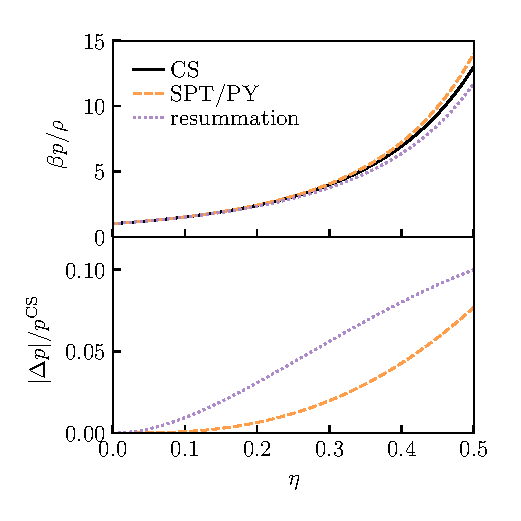
\includegraphics[width=0.9\linewidth,outer]{resummation-pressure}
  \caption[Accuracy of equation of state from partially resumming the virial series]{
    Equations of state for the single-component hard sphere liquid: Carnahan-Starling (CS), the scaled particle/Percus Yevick (SPT/PY) and the equation obtained from resumming terms in the virial series where there is a commong point of intersection.
    Top panel: pressure equations of state.
  Bottom panel: errors in the SPT/PY and resummation pressures are comparable across the whole liquid regime, taking the CS equation as the quasi-exact result.}
  \label{fig:resummation-pressure}
\end{SCfigure}

For single-component hard spheres the pressure obtained from the resummation in the previous section yields
\begin{equation}
  \frac{\beta p}{\rho} =
  \begin{cases}
    \frac{1}{1-\eta} & \; d=1 \\
    \frac{1}{(1-\eta)^2} & \; d=2 \\
    \frac{1 + \eta + (\frac{3\pi^2}{16} - 2) \eta^2}{(1-\eta)^3} & \; d=3.
  \end{cases}
\end{equation}
The resulting pressures for $d \le 2$ are identical to the scaled particle theory equations of state, where the first is the exact solution \eqref{eq:hard-rods-eos}.
For $d=3$ the resulting equation of state has a similar structure to the scaled particle theory solution (or equivalently the Percus-Yevick equation of state by the compressibility route) (SPT/PY) but it is slightly less accurate: at the freezing point $\eta_f \simeq 0.494$ the PY equation overestimates the pressure by $\sim7\%$ while for the above equation this is underestimated by $\sim11\%$, taking the Carnahan-Starling (CS) equation of state \cite{CarnahanJCP1969} as an estimate of the exact value.
The three equations of state mentioned are plotted together in Fig.\ \ref{fig:resummation-pressure} across the whole liquid regime in hard spheres.
While not exact, this shows that the morphometric contributions account for $\sim$90\% of the contributions to the equation of state which may suggest why morphological thermodynamics has been found to be highly accurate for descriptions of the hard sphere liquid \cite{RothPRL2006,LairdPRE2012,BlokhuisPRE2013,UrrutiaPRE2014,Hansen-GoosJCP2014,RobinsonPRL2019}.
This is discussed in more detail in the context of FMT in \cite{MarechalPRE2014}, and is partially attributable to cancellations of terms omitted from the resummation.

To account for the reduced accuracy of this equation of state for $d=3$ compared with PY, we observe that the PY hard sphere solution captures the third virial coefficient exactly, while this approach only provides a lower bound; the omitted configurations are known in the FMT literature as ``lost cases'' \cite{TarazonaPRE1997}.
A semi-empirical approach could reweight the final term in \eqref{eq:a3-d=3} to produce the third virial coefficient (if known), giving an equation of state for arbitrary mixtures of convex particles.
This reweighting is implicit in scaled particle theory and the Rosenfeld FMT functional \cite{TarazonaPRE1997,MarechalPRE2014}.

We see similar accuracy in the predicted surface tension at an infinite planar wall determined by $a_2$
\marginfootnote{This is true up to a normalisation constant, as $a_2$ conjugates with the intrinsic volume $V_2$ rather than the area $A = 2V_2$.
  The usual planar surface tension is thus obtained as $\gamma_\infty = a_2/2$.}.
The surface tension at an infinite planar wall is simply $a_2$ because it conjugates with the area.
In Ref.\ \cite{DavidchackMP2015} the results of extensive simulations measuring $a_2$ were parameterised by the following expression
\begin{equation}\label{eq:quasi-exact-surface-tension}
  %\begin{split}
  \beta a_2
  =
  \frac{1}{\pi \sigma^2} \left(
  \frac{\eta (2 + 3\eta - \frac{9}{5}\eta^2 - \frac{4}{5}\eta^3 - (5 \times 10^4) \eta^{20})}{(1 - \eta)^2}
  %% \right.
  %% \\
  %% &
  %% \left.
  %% \vphantom{\frac{1}{1}}
  - \ln{(1 - \eta)}
  \right),
  %\end{split}
\end{equation}
which we use to gauge the accuracy of predicted surface tensions.
We also compare the values of $a_2$ predicted by other morphometric theories of Ref.\ \cite{Hansen-GoosJPCM2006} (SPT/CS) and Ref.\ \cite{RobinsonPRE2019} (virial/CS).
The surface tensions are plotted in Fig.\ \ref{fig:resummation-a2}; the accuracy of the new result is comparable to SPT/PY in the liquid regime with the maximum error reaching $\sim12\%$.
Unsurprisingly, the other morphometric theories feature more accurate surface tensions; this is likely because they were constructed to satisfy thermodynamic relations which improves their accuracy.
%By contrast, the resummation route was not constructed for accuracy nor to satisfy thermodynamic relations.
Curiously, the error in the new theory scales almost identically to virial/CS theory at small $\eta$ even though the sign is different; all of the previous morphometric theories overestimate the surface tension, whereas the resummation route underestimates it.

\begin{SCfigure}
  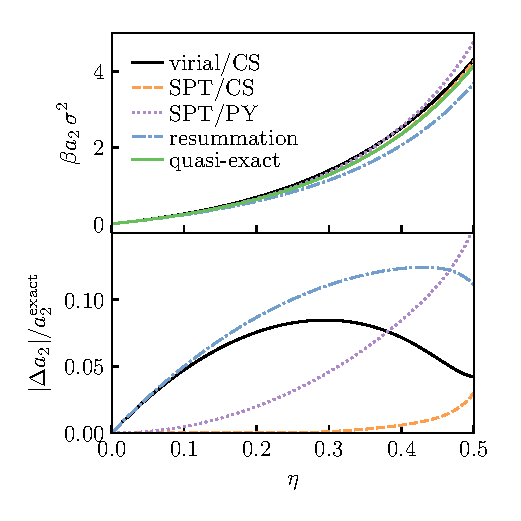
\includegraphics[width=0.9\linewidth,outer]{resummation-a2}
  \caption[Accuracy of surface tension from partially resumming the virial series]{
    Comparison of surface tensions for different morphometric theories.
  using the highly accurate result \eqref{eq:quasi-exact-surface-tension} from Ref.\ \cite{DavidchackMP2015} valid until $\eta \sim 0.5$.}
  \label{fig:resummation-a2}
\end{SCfigure}

%% \subsection{Beyond convex geometries and the choice of dividing surface}
%% \label{sec:general-geometries}

%% \begin{figure*}
%%   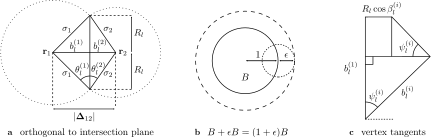
\includegraphics[width=0.65\linewidth,outer]{minkowski_addition}
%%   \caption{A dimer geometry considered in pair correlations in a fluid of $B$ particles showing (a) solute of two spheres $A$ generating an excluded volume $A \minkplus B$ and (b) the effective connected solute $A \minkplus B \minkminus B$.
%%   The exluded volume in each case is identical i.e.\ $A \minkplus B \minkminus B \minkplus B = A \minkplus B$.}
%%   \label{fig:minkowski_addition}
%% \end{figure*}

%% Until now we have focused on convex bodies, but we will now argue that the results apply for more general bodies.
%% In particular, for many-body correlations the ``solute'' consists of the disjoint union of particles see e.g.\ Fig.\ \ref{fig:system}.
%% We will determine necessary conditions for validity of the morphometric approach in in general solutes by examining the exact morphometric contributions described in previous sections.
%% A related problem is thermodynamic consistency for different choices of dividing surfaces in \eqref{eq:surface-tension}, which we will address in parallel.

%% Based on the exact results there are two ways the approach could fail:
%% \begin{enumerate}
%% \item For geometries where the integral geometric formula are invalid, e.g.\ the kinematic integrals, for non-convex geometries kinematic formula, and
%% \item Where the interaction with the solute cannot be reduced to the Euler characteristic, i.e.\ \eqref{eq:interactions-euler-equivalence}.
%% \end{enumerate}
%% As there are exact morphometric contributions to the free energy, a good approximation scheme should contain these; conversely, where these contributions are not captured provides necessary conditions for the scheme's validity.
%% We will address both potential failures in turn.

%% We used the kinematic integral \eqref{eq:binomial-kinematic-equation}, and its iterated form \eqref{eq:multinomial-kinematic-equation}, with convex bodies but it is valid for many more physically relevant geometries.
%% They can be extended \cite{Klain1997} to so-called \emph{polyconvex} bodies (also known as the convex ring), meaning any body formed by the countable union of convex objects.
%% This latter category covers most physically meaningful geometries, omitting pathological cases where size measures lose their meaning creating paradoxes \cite{BanachFM1924}.
%% The argument from Hadwiger's theorem similarly extends to polyconvex bodies.

%% Though the integral theorems hold for geometries of relevant physical interest, the equivalence between interaction and geometry \eqref{eq:interactions-euler-equivalence} may not.
%% We will consider two examples below in order to extend the geometric formalism to cases of physical interest.

%% First, consider the geometry formed by creating an infinitesimally small cavity inside a convex object.
%% Its Euler characteristic will deviate by $\pm 1$ (with sign dependent on dimension), however the interactions are unchanged because the cavity is not large enough to contain a finite-sized object.
%% In this case \eqref{eq:interactions-euler-equivalence} holds so long as the original convex geometry is used in place of the `true' body with the cavity.
%% %Going a step further, for finite-sized cavities able to contain a solvent particle, the cavity will be dynamically inaccessible to solvent particles (unless initially prepared inside) so the whole body can be treated as if it were solid, i.e.\ the interior of $\partial B$.

%% Next, we consider a geometry more typical of correlations in liquids: a dimer formed by two unit balls a distance $r$ apart i.e.\
%% \begin{equation*}
%%   A(r) = B^d \cup \mathcal{T}(r) B^d,
%% \end{equation*}
%% sketched in Fig.\ \ref{fig:minkowski_addition}.
%% This geometry is non-convex, and for $r > 1$ it is not even simply connected.
%% For interactions with a convex solvent particle $B$ we have possible Euler characteristics of intersection $\chi(A \cap B) \in \{0, 1, 2\}$ whereas $e^{-\beta u(A, B)} \in \{0, 1\}$, so it is not possible to establish an exact correspondence between the two.
%% We can proceed by determining an effective geometry where this relation does hold.
%% The exact result \eqref{eq:exact-mayer-exclusion} can be written
%% \begin{equation}
%%   \begin{split}
%%     e^{-\beta u(A, \mathcal{T} B)} - 1
%%     &= -\chi((A \minkplus B) \cap \{\vec{r}\}) \\
%%     &= -\chi((A \minkplus B \minkminus B) \cap B),
%%   \end{split}
%% \end{equation}
%% with the last line valid so long as $A \minkplus B \minkminus B = \{\vec{c} \, | \, (\vec{c} \minkplus B) \subseteq A \minkplus B\}$ is simply connected, otherwise the Euler characteristic of the intersecting geometry can be greater than one $\chi((A \minkplus B \minkminus B) \cap B) > 1$.
%% The effective geometry $A \minkplus B \minkminus B$ recovers the correspondence between interaction and geometry \eqref{eq:interactions-euler-equivalence}.
%% Addition (dilation) and subtraction (erosion) operations are not inverse operations so $A \minkplus B \minkminus B \ne A$, however $A \minkplus B \minkminus B \minkplus B = A \minkplus B$ so $A \minkplus B \minkminus B$ acts as an effective generator of the exclusion region.
%% The effective geometry for the previous example, a nearly convex body with an infinitesimal cavity, recovers the convex object.

%% Related to the above discussion is the effect of the choice of dividing surface on the decomposition of surface and volume terms in \eqref{eq:surface-tension}.
%% The thermodynamics should not depend on the choice of boundary, i.e.\ we can define a functional working with the parallel surface
%% \begin{equation*}
%%   \Delta \Omega'[A \minkplus \epsilon B]
%%   =
%%   \sum_{k=0}^d a_k' V_k(A \minkplus \epsilon B)
%% \end{equation*}
%% but thermodynamic consistency requires
%% \begin{equation*}
%%   \Delta \Omega[A] =
%%   \Delta \Omega'[A \minkplus \epsilon B].
%% \end{equation*}
%% A controlled expansion of the solvation energy which allows for different choices of dividing surface must be invariant to the particular choice.
%% The transformation between the coefficients $\{a_k\}$ and $\{a'_k\}$, which we give explicitly in Appendix~\ref{appendix:parallel-surfaces}, are straightforward which is a particular strength of using the morphometric \emph{ansatz}.
%% When this transformation fails leading to inconsistent thermodynamics, we know the theory has failed.
%% We find a necessary condition for the theory's validity is thus that $\chi(A \minkplus B^d \minkminus B^d) = \chi(A \minkplus B^d)$.

%% The boundary of the effective volume $\partial(A \minkplus B \minkminus B)$ is commonly called the \emph{molecular surface} \cite{?}, while the boundary of the excluded volume $\partial(A \minkminus B)$ is referred to as the \emph{solvent accessible surface}.
%% There is also an infinite family of equivalent parallel surfaces in between i.e.\ $\partial(A \minkplus B \minkminus \epsilon B)$ for $\epsilon \in [0, 1]$ but the two extremes are the most natural choices.
%% When the boundary of the effective geometry (molecular surface) self-intersects, we expect the theory to break down.
%% In the previous example this occurs at $r = 2\sqrt{3}$ for spherical solvent particles $B = B^d$ \cite{OettelEL2009}.
%% At this point, descriptions with different choices of boundary become inconsistent.
%% Consider the Euler characteristic of the effective body (molecular surface)
%% \begin{equation}
%%   \chi(A \minkplus B^d \minkminus B^d)
%%   =
%%   \begin{cases}
%%     1 & r < 2\sqrt{3} \\
%%     2 & r > 2\sqrt{3}
%%   \end{cases}
%% \end{equation}
%% whilst for the parallel volume (solvent accessible surface)
%% \begin{equation}
%%   \chi(A \minkplus B^d)
%%   =
%%   \begin{cases}
%%     1 & r < 2 \\
%%     2 & r > 2
%%   \end{cases}
%% \end{equation}

\section{Discussion}

%We have derived the morphometric solvation free energy for mixtures of hard convex particles from first-principles using the virial series.

While the morphometric theory we have derived from the virial series is less accurate than theories obtained from other routes. 
Specifically, in $d=3$ the pressure and surface tension is comparable in accuracy to the classic SPT/PY route and in $d=2$ the two approaches are equivalent.
\todo{Check that surface tension in $d=2$ is the same as SPT.}
However, the usefulness of the new route is extends beyond mere accuracy; the free energy we have identified emerges \emph{rigorously} as a contribution from the virial series.
The fact that this exact contribution is still reasonably accurate suggests that the corrections to it are small, providing further justification of the morphometric approach.
This means we could write the insertion cost for a solute $K$ as the \emph{exact} decomposition
\begin{equation}\label{eq:exact-morph-decomposition}
  \Delta \Omega[K]
  =
  \sum_{k=0}^d a_k V_k(K)
  + \Delta \Omega_\mathrm{extra}[K]
\end{equation}
with coefficients $a_k$ as previously calculated, and $\Delta \Omega_\mathrm{extra}$ contains the remaining contributions.
Notably the exponentially damped oscillations occuring in pair correlations at asymptotically large separations must be contained within $\Delta \Omega_\mathrm{extra}$.
The insertion cost is known to contain singularities \cite{ReissJCP1959} so it is unlikely that $\Delta \Omega_\mathrm{extra}$ possesses a simple analytic form.
It is possible that additional exact morphometric contributions exist, and they would be contained in $\Delta \Omega_\mathrm{extra}$ also.

Furthermore, the formal derivation we have followed naturally leads to explicit expressions for $\Delta \Omega_\mathrm{extra}$.
The next leading contribution from the virial series would be:
\begin{equation}
  \Delta \Omega_\mathrm{extra}[K]
  =
  \frac{\rho^2}{2}
  \sum_{s_1=1}^m \sum_{s_2=1}^m
  x_{s_1} x_{s_2}
  \left(
  \int_{G_d^2} \chi(K \cap g_1 K_{s_1}) \chi(K \cap g_2 K_{s_2}) \chi(g_1 K_{s_1} \cap g_2 K_{s_2}) dg_1 dg_2
  - \Lambda_{s_1,s_2} \right)
  + \mathcal{O}(\rho^3),
\end{equation}
which involves a \emph{ring integral}.
These integrals can be calculated straightforwardly in hard spheres \cite{MontrollJCP1941}, or using the Radon transform for convex geometries of arbitrary shapes \cite{WertheimMP1994,WertheimMP1996,WertheimMP1996a}.
Corrections could be systematically included by further resummations over topologically identical integrations, with ring integrals as the leading order terms.
The integral corrections are discussed in Ref.\ \cite{MarechalPRE2014} in the context of free energy functionals for inhomogeneous liquids; our system is effectively homogeneous so we expect it to be easier to construct a theory with higher-order terms.

The form of the exact contribution is instructive in how it applies to mixtures.
It is argued in Ref.\ \cite{KodamaJCP2011} that for an $m$-component mixture the appropriate morphometric form reads
\begin{equation}\label{eq:morphometric-approach-mixtures}
  \Delta \Omega
  =
  \sum_{i=1}^m
  a_3^{(i)} V_i
  + a_2^{(i)} A_i
  + a_1^{(i)} C_i
  + a_0^{(i)} X_i
\end{equation}
where the coefficients $a_k^{(i)}$ now depend on the specific interactions with each species and their composition, and $\{V_i, A_i, C_i, X_i\}$ are geometric measures on some composite body of the solute with solvent particles of species $i$, e.g.\ their specific exluded volume.
By contrast, our exact morphometric contribution does not involve different intrinsic volumes for the different cross-species interactions, suggesting \eqref{eq:morphometric-approach} is a general enough \emph{ansatz} and the extension for mixtures \eqref{eq:morphometric-approach-mixtures} proposed in Ref.\ \cite{KodamaJCP2011} may be unnecessary.

In addition to the accuracy of the exact contribution, we can argue against the alternative morphometric form for mixtures \eqref{eq:morphometric-approach-mixtures} by considering the polydisperse mixture limit.
The alternative form contains $4m$ parameters which becomes underconstrained in the polydisperse limit $m \to \infty$, so it is unlikely that the coefficients $a_k^{(i)}$ can be totally independent.
More precisely, thermodynamic consistency of the (osmotic) pressure requires
\begin{equation}\label{eq:osmotic-consistency-1}
  \begin{split}
    \beta p
    &=
    \rho - \beta f^\mathrm{ex}
    + \rho \left( \frac{\partial \beta f^\mathrm{ex}}{\partial \rho} \right)_{V,T}
    \\
    &=
    \rho - \beta f^\mathrm{ex}
    + \rho \sum_{i=1}^m
    x_i \left( \frac{\partial \beta f^\mathrm{ex}}{\partial x_i} \right)_{V,T}
  \end{split}
\end{equation}
where $f^\mathrm{ex} = F^\mathrm{ex}/V$ is the (excess) free energy density.
The latter line, valid in the case of mixtures, becomes poorly defined in the polydisperse limit $m \to \infty$ with $x_i \to 0$.
To remain well-defined for polydisperse systems the composition dependence of the free energy should reduce to a (finite) set of \emph{weighted densities} \cite{GualtieriJCP1982, WarrenPRL1998, SollichPRL1998, SollichAiCP2001}.
This is the case for our virial-derived approach where the density dependence enters through scaled particle variables $\{\xi_k\}$, so \eqref{eq:osmotic-consistency-1} becomes
\begin{equation}\label{eq:osmotic-consistency-2}
  \beta p
  =
  \rho - \beta f^\mathrm{ex}
  + \sum_k
  \xi_k \left( \frac{\partial \beta f^\mathrm{ex}}{\partial \xi_k} \right)_{V,T}.
\end{equation}
To demonstrate that our form works for both discrete and continuous (polydisperse) mixtures, we rewrite the geometric parameters \eqref{eq:spt-variables} in the more general form
\begin{equation}
  \xi_k
  =
  \rho \int \widetilde{V}_k(K_s) d\mu(s),
\end{equation}
introducing the probability measure $\mu(s)$ for the molarities of particle species/shapes such that $\int d\mu(s) = 1$.
This reduces to the previous form for discrete mixtures if we set $\mu(s)$ to the counting measure, however in integral form we are free to extend the calculation to continuous mixtures.

As an example we consider a polydisperse mixture of particles of reference shape $K$ with uniformly distributed sizes $s \in [s_0, s_1]$ giving $V_k(K_s) = V_k(s K) = s^k V_k(K)$, then
\begin{equation}
  \begin{split}
    \xi_k
    &=
    \rho \widetilde{V}_k(K) \int_{s_0}^{s_1} s^k ds
    \\ &=
    \rho \widetilde{V}_k(K) \left(\frac{s_1^{k+1} - s_0^{k+1}}{k+1}\right).
  \end{split}
\end{equation}
Inserting this reweighted volume into the explicit expressions given in the appendix yields new thermodynamic coefficients for uniformly distributed polydisperse mixtures.
The composition dependence enters only through moments of the size distribution guaranteeing a well-defined free energy, detailed discussion of which can be found in Refs.\ \cite{GualtieriJCP1982,WarrenPRL1998,SollichPRL1998,SollichAiCP2001}.

\section{Summary}

We have derived an exact morphometric contribution for a general class of hard particle liquids by resumming terms in the virial series.
Previous studies have primarily used FMT to develop morphometric theories, so we have successfully developed an independent justification for the morphometric approach as the leading term in a controlled expansion.
The exact result applies for mixtures of hard convex particles in an isotropic phase.

%This result is not that surprising as the morphometric approach can be obtained as a limit case of FMT \cite{Hansen-GoosJPCM2006}, which itself can be formulated as the resummation of the same terms in the virial expansion \cite{LeithallPRE2011,KordenPRE2012,MarechalPRE2014}.

In hard spheres the exact contribution features similar accuracy as scaled particle theory, so it captures most contributions to the bulk free energy and seems to be why the approach has been successful.
Though as noted in Ref.\ \cite{MarechalPRE2014} this is partially due to a cancellation in the omitted terms of the virial expansion, so it may still desirable to improve the morphometric approach by inclusion of additional terms.
The exact morphometric contribution provides a suitable starting point for including additional terms to improve accuracy.

%\appendix*

\section{Explicit morphometric contributions in the virial expansion}
%\label{appendix:lambda}

Here we explicitly evaluate the contributions in the virial expansion from configurations sharing a common point of intersection via \eqref{eq:little-lambda}.

For $d=1$ the index runs over $k \in \{0,1\}$, giving condition on the summation indices $N_0 = k$ and $N_1 = n - N_0$ leading to a single term for each value of $k$:
\begin{subequations}
  \label{eq:little-lambda-d=1}
  \begin{align}
    \lambda_0^{(n)} &= \xi_1^n
    \\
    \lambda_1^{(n)} &= n \xi_0 \xi_1^{n-1}.
  \end{align}
\end{subequations}
For $d=2$ we have $k \in \{0,1,2\}$, with summation conditions $2N_0 + N_1 = k$ and $N_2 = n - N_1 - N_0$ giving:
\begin{subequations}
  \label{eq:little-lambda-d=2}
  \begin{align}
    \lambda_0^{(n)} &= \xi_2^n
    \\
    \lambda_1^{(n)} &= n \xi_1 \xi_2^{n-1}
    \\
    \lambda_2^{(n)} &=
    n \xi_0 \xi_2^{n-1}
    + \frac{n(n-1)}{2} \xi_1^2 \xi_2^{n-2}.
  \end{align}
\end{subequations}
Finally, for $d=3$ we have $k \in \{0,1,2,3\}$, with summation conditions $3N_0 + 2N_1 + N_2 = k$ and $N_3 = n - N_2 - N_1 - N_0$ giving:
\begin{subequations}
  \label{eq:little-lambda-d=3}
  \begin{align}
    \lambda_0^{(n)} &= \xi_3^n
    \\
    \lambda_1^{(n)} &= n \xi_2 \xi_3^{n-1}
    \\
    \lambda_2^{(n)} &=
    n \xi_1 \xi_3^{n-1}
    + \frac{n(n-1)}{2} \xi_2^2 \xi_3^{n-2}
    \\
    \lambda_3^{(n)} &=
    n \xi_0 \xi_3^{n-1}
    + n(n-1) \xi_1 \xi_2 \xi_3^{n-2}
    \nonumber \\ & \qquad
    + \frac{n(n-1)(n-2)}{6} \xi_2^3 \xi_3^{n-3}.
  \end{align}
\end{subequations}

We will now resum $\lambda_k^{(n)}$ over $n$ in order to determine the values of $a_k$ for $d \le 3$.
For $d=1$ we insert \eqref{eq:little-lambda-d=1} into \eqref{eq:final-a-coefficient}:
\begin{subequations}
  \begin{align}
    \beta a_0
    &= - \ln{(1 - \eta)},
    \\
    \beta p =
    \beta a_1 &=
    \frac{2 \xi_0}{1-\eta},
  \end{align}
\end{subequations}
with $\xi_0 = \rho / 2$ giving the exact result for hard rods \eqref{eq:hard-rods-morphometric} and \eqref{eq:hard-rods-eos}.
For $d=2$ we insert \eqref{eq:little-lambda-d=2} into \eqref{eq:final-a-coefficient}:
\begin{subequations}
  \begin{align}
    \beta a_0 &= -\ln{(1 - \eta)},
    \\
    \beta a_1 &= \frac{2 \xi_1}{1-\eta},
    \\
    \beta p =
    \beta a_2 &=
    2\pi \left(
    \frac{\xi_0}{1-\eta}
    + \frac{\xi_1^2}{2(1-\eta)^2}
    \right).
  \end{align}
\end{subequations}
Note: for hard discs of diameter $\sigma$ we obtain $V_1 = \pi \sigma / 2$ so $\xi_0 = \rho / (2\pi)$ and $\xi_1 = \rho \sigma / 2$ for the single-component fluid.
Finally, for $d=3$ we insert \eqref{eq:little-lambda-d=3} into \eqref{eq:final-a-coefficient}:
\begin{subequations}
  \begin{align}
    \beta a_0 &= -\ln{(1 - \eta)},
    \\
    \beta a_1 &= \frac{2 \xi_2}{1-\eta},
    \\
    \beta a_2 &=
    2 \pi
    \left(
    \frac{\xi_1}{1-\eta}
    + \frac{\xi_2^2}{2(1-\eta)^2}
    \right),
    \\
    \beta p =
    \beta a_3 &=
    8 \pi\left(
    \frac{\xi_0}{1-\eta}
    + \frac{\xi_1 \xi_2}{(1-\eta)^2}
    + \frac{\xi_2^3}{3 (1-\eta)^3}
    \right).
    \label{eq:a3-d=3}
  \end{align}
\end{subequations}
Note: for hard spheres of diameter $\sigma$ we obtain $V_1 = 2\sigma$ and $V_2 = \pi \sigma^2 / 2$ so $\xi_0 = \rho / (8\pi)$, $\xi_1 = \rho \sigma / (2\pi)$ and $\xi_2 = \rho \pi \sigma^2 / 8$ for the single-component fluid.
In the above steps we have used the fact that $\xi_d = \eta$ to simplify the resulting expressions.

\ifdefined\includebibliography
  \printbibliography
\fi

\end{document}

%TC: macro \marginfootnote [other]
%TC: envir SCfigure [] other
%TC: macrocount beginSCfigure [figure]
\documentclass[11pt,twoside]{report}
\usepackage{preamble}
\setcounter{chapter}{5}
\graphicspath{{../img/}}
\def\includebibliography{}

\begin{document}
\chapter{Nucleation kinetics in simple drying aerosols}
\epigraph{Remove the plastic.}{Sears\textsuperscript{\textregistered} cross-trainer manual.}
\label{chapter:aerosols}

In previous chapters we focused on modelling hard spheres at high densities, with a particular focus on supercooled liquids and glasses.
As we mentioned in the introduction, another central topic of the high density liquid is the process of nucleation by which the liquid becomes a crystal.
This chapter addresses nucleation within the context of drying aerosol droplets, with applications to climate modelling and industrial spray drying.
The chemistry involved in aerosols makes this system much more complicated than can be captured with a simple hard sphere interaction, so our microscopic morphometric formalism will not work here at present.
Instead, we start from the mesoscale limit where the droplet can be treated as a continuum.
%% At present real systems are too complex to be treated from first principles, so we will employ phenomenological fits to available data assuming classical nucleation theory.
%% We hope one day theory will allow a connection between microscopic and mesoscopic approaches, paving the way to a properly first-principles treatment of real systems.

This work was undertaken in collaboration with members of the Reid group in the School of Chemistry at the University of Bristol.
In particular, the experiments were carried out by Flo Gregson.
My contribution to this work was through theory and numerical modelling to better understand the experimental data.
Consequently, while I will describe the experiments the focus of the chapter will be theoretical.
Some of this work has already been published in Ref.\ \cite{GregsonJPCB2019}, and we hope to publish the remainder as Refs.\ \cite{RobinsonTBD2019,GregsonTBD2019} later this year.

Finally, for the benefit of those working in the field of supercooled liquids and glasses who are reading this and wondering what this chapter has to do with the rest of the thesis, we put forward the following additional motivation: in order to finally solve the glass transition, we must address the looming climate crisis to keep glass researchers alive long enough to actually reach a consensus%
\marginfootnote{On second thought, I suppose another option would be: ``last statistical physicist alive gets to decide the nature of the glass transition''.}[-2cm].
As such, consider this chapter a small step in consensus building.

\section{Introduction}

The impact of atmospheric aerosols on the climate remains the leading single uncertainty in climate predictions \cite{BoucherIPCC2013,CarslawN2013,LeePNAS2016,RegayreACP2018}.
In particular, the radiative forcing caused by anthropogenic aerosols in clouds features large uncertainties due to the difficulty of direct measurement, and the large parameter spaces of theoretical models \cite{LeePNAS2016}.
Thus, the importance of improving models for atmospheric aerosols to better predict climate change and inform policy cannot be overstated.
In addition, atmospheric aerosols have potential applications in geoengineering \cite{PringleACP2012}.

Notably, radiative forcing of atmospheric aerosols is stongly influenced by their optical properties \cite{HodasACP2015,CotterellACP2017}.
The solute concentration and physical state (i.e.\ whether it is crystalline or amorphous) can thus have a dramatic effect on climate predictions.
Central to this is the nucleation and drying kinetics of atmospheric droplets.
Where aerosols are included in climate models the focus is typically on sulphates \cite{MannACP2014,ZhuNC2019}.
However, sea salt aerosols (e.g.\ those containing \ce{NaCl}), deposited into the atmosphere through natural processes, are more prevalent in the atmosphere than sulphates making up the second largest component of atmospheric aerosols by mass \cite{KeeneJAS1998}; a major component of aged \ce{NaCl} aerosols is sodium nitrate (\ce{NaNO3}) formed through reactions with nitrogen oxides \cite{TolockaJPCA2004}, a significant industrial emission.
Subsequent reactions form secondary organic aerosols which further impact the climate \cite{ScottACP2014,PoschlCR2015} and are associated with adverse health effects \cite{PoschlCR2015}.
Given their abundance and relative simplicity we focus on \ce{NaCl} and \ce{NaNO3} aerosol droplets.

Understanding the droplet drying and crystallisation process is also important for industrial applications, most notably in spray-drying.
The goal in these applications is to control the distribution of sizes, morphology and phase of the final droplets, which are very sensitive to processing conditions such as solvent \cite{CarverIECR2012,LintingreSM2016}, temperature \cite{IveyAST2018,YouDT2014,LinPT2015}, pH \cite{YuJPS2002,DubbiniIJP2014} and additional co-excipients \cite{ZhongAP2018,NandiyantoAPT2011,LyuJCG2017}.
Tailoring crystallisation is particularly important because crystal and amorphous states have fundamentally different properties: crystalline droplets are typically more stable, suitable for e.g.\ product storage \cite{VehringJAS2007,CostantinoJPS1998}, whereas amorphous droplets are more soluble which is desirable for e.g.\ drug delivery \cite{AmstadJPCB2016,BroughIJP2013}.
Our investigation of crystal nucleation rates can be inverted to design spray-drying conditions to achieve a desired final state.

In this chapter we will investigate drying and crystal nucleation of free aerosol droplets, by combining experiments and a numerical model of free aerosol droplets.
The experiments are described in section \ref{sec:experiments}, and we report matching them to a diffusional model of droplet evolution in section \ref{sec:evolution}.
We find that classical nucleation theory accurately predicts the crystallisation times for \ce{NaCl} aerosols, but not for \ce{NaNO3}, in section \ref{sec:nucleation}.
For \ce{NaNO3} we report nucleation rates with non-monotonic behaviour with increasing solute concentration.

\section{Experiments}
\label{sec:experiments}

The kinetics of drying \ce{NaCl} and \ce{NaNO3} droplets was measured using the Comparative-Kinetics Electrodynamic Balance (CK-EDB).
In all experiments HPLC-grade water, BioXtra $\ge 99.5\%$ \ce{NaCl} (Sigma-Aldrich) and analytic grade \ce{NaNO3} (Fisher-Scientific) were used.
The CK-EDB instrument has been detailed in previous work \cite{DaviesAST2012} so we will only describe it briefly here.
Droplets of known concentration are produced by a droplet-on-demand generator (MicroFab) and injected into the CK-EDB instrument.
Upon generation the droplets are charged ($<\SI{10}{\femto\coulomb}$ through e.g.\ an ionic imbalance) with an induction electrode such that they become trapped within the centre of the electrodynamic field, produced by the application of an AC field between two sets of concentric cylindrical electrodes.
An additional DC field is applied to the lower set of electrodes to counteract gravity and drag forces acting on the droplet.
A circulating current of ethylene glycol coolant across the electrodes controls the chamber temperature $T_{\infty}$ in the range 273--\SI{323}{\kelvin}.

To determine the size and physical state of the droplet, it is illuminated with a \SI{532}{\nano\metre} continuous-wave laser.
The resulting scattering pattern is recorded by a CCD camera placed at \SI{45}{\degree} to the beam over an angular range of $\SI{\sim24}{\degree}$.
For isotropic droplets in a liquid or dried amorphous state the droplet radius $R$ determines the angular separation between the fringes in the pattern $\Delta \theta$.
Assuming the geometric optics approximation of Mie theory, this relationship is given by
\begin{equation*}
  R
  =
  \frac{\lambda}{\Delta \theta} \left(
  \cos{\left(\frac{\theta}{2}\right)}
  + \frac{n \sin{\left(\frac{\theta}{2}\right)}}{\sqrt{1 + n^2 - 2n \cos{\left(\frac{\theta}{2}\right)}}}
  \right)^{-1}
\end{equation*}
where $\lambda$ is the laser wavelength, $\theta$ is the central viewing angle and $n$ is the droplet refractive index.
This approximation scheme determines the droplet radius within an accuracy of $\SI{\pm100}{\nano\metre}$.
This method fails when crystallisation occurs breaking isotropy and the scattering pattern dramatically changes; this feature allows the time of crystallisation to be determined to within $\SI{\sim10}{\milli\second}$.
Nucleation and growth occur on such a short time scale that it is not possible to obtain information from the experiments on where inside the droplet this occurs or how many initial nucleation sites there were; we can only determine that the droplet has nucleated crystals.

The instrument features two gas flows for wet and dry nitrogen applied to the droplet at a rate of \SI{0.03}{\metre\per\second}.
Controlling the ratio of these two flows through a mass-flow controller (MKS instruments) sets the relative humidity (RH) inside the CK-EDB chamber.
Liquid aqueous \ce{NaCl} and aqueous \ce{NaNO3} droplets (20\% solute concentration by weight) were evaporated into dry conditions at \SI{20}{\celsius}.
Crystallisation of multiple \ce{NaCl} droplets occurred reproducibly \SI{1}{\second} after droplet generation \cite{GregsonJPCB2019}, whereas \ce{NaNO3} droplets showed stochastic behaviour with a fraction of droplets not crystallising over the timescale of the experiment (droplets were typically trapped for \SI{10}{\second}).
The stochastic behaviour persists when the experiment was repeated for the \emph{same} \ce{NaNO3} droplet over a cycle of repeatedly lowering and raising the RH (described in more detail in Ref.\ \cite{GregsonTBD2019}), ruling out impurity-driven heterogeneous nucleation.

\begin{SCfigure}
  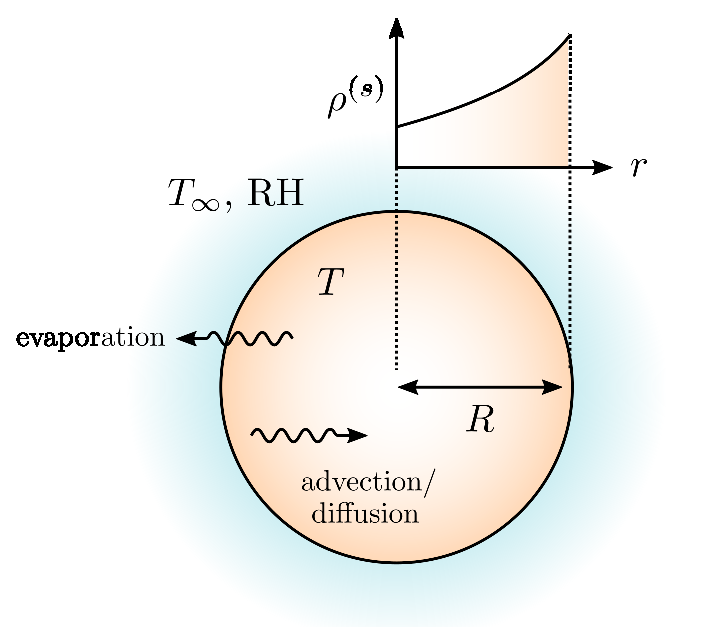
\includegraphics[width=0.75\linewidth,outer]{aerosol-droplet}
  \caption[Model drying aerosol droplet]{
    A drying droplet solution of radius $r=R(t)$ surrounded by a gas of temperature $T_\infty$ and relative humidity RH.
    Evaporation of the solvent (water) causes the droplet to shrink and surface enrichment of solute concentration $\rho^{(s)}$ together with evaporative cooling $T < T_\infty$.}
  \label{fig:aerosol-droplet}
\end{SCfigure}

Follow up experiments by the Reid group placed the droplets inside a scanning electron microscope (SEM) for imaging.
These found that for \ce{NaCl} aerosols nucleation seems to occur at the boundary%
\marginfootnote{I am reversing chronology here: actually, we used our numerical model to predict this \emph{first}, which was then was confirmed by SEM images.}.
The experiments featuring slower evaporation tended to have more perfect crystals suggesting there were fewer nucleation sites, whereas the more rapidly evaporating droplets showed imperfections consistent with there being multiple nucleation sites at the boundary \cite{GregsonTBD2019}.
The SEM results for \ce{NaNO3} were inconclusive, although the resulting crystals were more spherical suggesting there were multiple nucleation sites which may be less strongly distributed at the boundary.

\section{Model for a drying droplet}
\label{sec:evolution}

\subsection{Overview and notation}

In order to obtain nucleation rates we require the time evolution of the droplet's concentration profile over its drying history, and a phenomenological model for nucleation rates based on concentration.
To determine the concentration profile trajectory for a drying droplet we have to consider the relative motion of solute and solvent species inside the droplet, of various species in the surrounding vapour phase, as well as the evaporation of solvent across the phase boundary.
Our approximations will reduce this to a moving boundary problem with solely diffusional mixing.

Prior to crystallisation a drying droplet will be approximately spherical, so we consider a phase boundary at radius $R(t)$ evolving in time $t$.
Writing the distance from the center of the droplet as $r$, the phase boundary separates the liquid phase inside $r \in [0, R(t))$ from the vapour phase outside $r \in (R(t), \infty]$.
The droplet is sketched in Fig.\ \ref{fig:aerosol-droplet}.
%In the experiments are performed in ambient conditions so the surrounding gas is strictly speaking a mixture, but to a reasonable approximation we can treat it as a single component.

We label the solute and (ambient) gas components as $s$ and $g$ respectively, and the evaporating solvent component as $f$ for \emph{fluid} as it exists in both the liquid and gas phases.
The density is $\rho = \sum_i \rho^{(i)}$ where the (mass) concentration of each component is $\rho^{(i)}$ for $i \in (f,s)$ in the droplet and $i \in (f,g)$ in the gas.
A useful auxillary variable is the mass fraction of each component, i.e.\
\begin{equation}\label{eq:mass-fraction}
  Y^{(i)} = \frac{\rho^{(i)}}{\rho}.
  %{\sum_j \rho^{(j)}}
  %{\rho^{(f)} + \rho^{(s)}}
  %\frac{\rho^{(i)}(\vec{r})}{\rho^{(f)}(\vec{r}) + \rho^{(s)}(\vec{r})}
  %\qquad i \in \{f, s\}.
\end{equation}
%with $j$ running over the components of the relevant phase.
%Clearly $Y^{(f)} = 1 - Y^{(s)}$
As both phases are binary mixtures%
\marginfootnote{This is not strictly true.
  The liquid phase is certainly a binary mixture of solvent and solute, however the vapour is composed of the evaporated solvent and a multicomponent ambient gas phase.
  However, we can treat the ambient gas as an effectively single-component system to a very good approximation.}[-1.5cm]
so we only need to solve for one component; we choose to solve for the solute mass fraction $Y^{(s)}$ in the droplet and the solvent mass fraction $Y^{(f)}$ in the surrounding vapour.

The thermal conductivity of liquids is generally much larger than the mass diffusivity, so to leading order we can treat temperature $T$ as homogeneous throughout the droplet.
This approximation neglects potential conduction forces driven by temperature gradients.
The droplet temperature will be smaller than the ambient temperature $T_\infty$ because vaporisation carries a latent heat
We will determine $T$ through the rate of vaporisation which will be moderate the vaporisation rate and enter into the nucleation calculations.
However, as a simplification we do not incorporate this temperature into the dynamics themselves through modified diffusion coefficients.

\subsection{Evolution of the concentration profile}

In the absence of any chemical reactions the continuity equation for each species component reads
\begin{equation}\label{eq:species-continuity}
  \frac{\partial \rho^{(i)}}{\partial t} +
  \vec{\nabla} \cdot (\rho^{(i)} \vec{v}^{(i)}) = 0
  \qquad i \in \{f,s\}
\end{equation}
where $\vec{v}^{(i)}$ is the velocity of species $i$, or in terms of relative flows
%% and the mass-averaged fluid velocity is
%% \begin{equation}
%%   \vec{v} = \sum_i Y^{(i)} \vec{v}^{(i)}
%% \end{equation}
%% We have
%% \begin{equation*}
%%   \frac{\partial \rho^{(i)}}{\partial t} +
%%   \vec{\nabla} \cdot (\rho^{(i)} \vec{v}) +
%%   \vec{\nabla} \cdot (\rho^{(i)} (\vec{v}^{(i)} - \vec{v})) = 0
%%   \qquad i \in \{f,s\}
%% \end{equation*}
%% and defining the relative mass flux as
%% \begin{equation}\label{eq:relative-mass-flux}
%%   \vec{j}^{(i)} = \rho^{(i)} (\vec{v}^{(i)} - \vec{v})
%%   \qquad i \in \{f,s\}
%% \end{equation}
%% gives
\begin{equation}\label{eq:species-continuity-relative}
  \frac{\partial \rho^{(i)}}{\partial t} +
  \vec{\nabla} \cdot (\rho^{(i)} \vec{v}) +
  \vec{\nabla} \cdot \vec{j}^{(i)} = 0
  \qquad i \in \{f,s\}
\end{equation}
where the mass-averaged fluid velocity is $\vec{v} = \sum_i Y^{(i)} \vec{v}^{(i)}$ and the relative mass flux is $\vec{j}^{(i)} = \rho^{(i)} (\vec{v}^{(i)} - \vec{v})$.
Any advective/convective flows will typically be contained in $\vec{v}$, while diffusive effects are captured by $\vec{j}^{(i)}$.

Volume additivity holds to a good approximation \cite{HandscombCES2009}, i.e.\ the density and concentrations are related by
\begin{equation}\label{eq:volume-additivity}
  %\begin{split}
  \frac{1}{\rho} =
  \frac{Y^{(s)}}{\rho_0^{(s)}} + \frac{Y^{(f)}}{\rho_0^{(f)}}
  %% \sum_{k \in \{f,s\}} \frac{Y^{(k)}}{\rho^{(j)}_0} \\
  %% &=
  %% \frac{Y^{(i)}}{\rho^{(i)}_0} +
  %% \frac{1 - Y^{(i)}}{\rho^{(j)}_0}
  %% \qquad i,j \in \{f,s\}, \; j \ne i.
  %\end{split}
\end{equation}
where $\rho_0^{(s)}$ and $\rho_0^{(f)}$ are the densities of the pure substances in the liquid phase; as no stable amorphous phases of \ce{NaCl} or \ce{NaNO3} are known we approximate $\rho_0^{(s)}$ by the density in the crystal phase.

By considering mass conservation one obtains
\begin{equation*}
  \vec{\nabla} \cdot \vec{v}
  =
  \frac{1}{\rho^2}
  \frac{\partial \rho}{\partial Y^{(s)}}
  \vec{\nabla} \cdot \vec{j}^{(s)}
\end{equation*}
so assuming volume additivity \eqref{eq:volume-additivity} we can define the mass difference parameter as
\begin{equation}\label{eq:lambda}
  \Lambda
  =
  \frac{1}{\rho^2} \frac{\partial \rho}{\partial Y^{(s)}} \\
  =
  \frac{1}{\rho^{(f)}_0} -
  \frac{1}{\rho^{(s)}_0}
\end{equation}
giving $\vec{v} = \Lambda \vec{j}^{(s)}$.
This simplifies the advective term in the continuity equation \eqref{eq:species-continuity-relative} leading to
\begin{equation}\label{eq:species-continuity-relative-without-advection}
  \frac{\partial \rho^{(s)}}{\partial t} +
  \vec{\nabla} \cdot \left(
  (1 + \Lambda \rho^{(s)}) \, \vec{j}^{(s)}
  \right) = 0.
\end{equation}
For the relative mass flux we assume Fick's law for diffusion
\begin{equation}\label{eq:ficks-law}
  \vec{j}^{(i)} = -D_\mathrm{eff} \rho \vec{\nabla} Y^{(i)},
\end{equation}
where $D_\mathrm{eff}$ is an effective \emph{binary} diffusion constant for the relative motion.
Inserting \eqref{eq:ficks-law} into \eqref{eq:species-continuity-relative-without-advection} and using the product rule, i.e.\
\begin{equation*}
  %% \begin{split}
  \vec{\nabla} \rho^{(s)}
  =
  %% \vec{\nabla} \left( \rho Y^{(s)} \right)
  %% &=
  %% \rho \vec{\nabla} Y^{(s)}
  %% + Y^{(s)} \vec{\nabla} \rho
  %% \\ &=
  %% \rho \vec{\nabla} Y^{(s)}
  %% + Y^{(s)} \frac{\partial \rho}{\partial Y^{(s)}} \vec{\nabla} Y^{(s)}
  %% \\ &=
  %% \rho \vec{\nabla} Y^{(s)}
  %% + \Lambda Y^{(s)} \rho^2 \vec{\nabla} Y^{(s)}
  %% \\ &=
  \left(
  1 +
  \Lambda \rho^{(s)}
  \right)
  \rho
  \vec{\nabla} Y^{(s)}.
  %% \end{split}
\end{equation*}
Finally, this gives the standard diffusion equation
\begin{equation}\label{eq:final-diffusion}
  \frac{\partial \rho^{(s)}}{\partial t}
  =
  \vec{\nabla} \cdot \left(
  D_\mathrm{eff} \vec{\nabla} \rho^{(s)}
  \right)
\end{equation}
where the advective forces have vanished providing a convenient form for numerical implementation.
By comparison, the mass fraction is widely used in the literature (e.g.\ Ref.\ \cite{HandscombCES2009}) which leads to separate advection and diffusion terms i.e.\
\begin{equation*}
  \rho \left(
  \frac{\partial Y^{(s)}}{\partial t} +
  \underbrace{\vec{v} \cdot \vec{\nabla} Y^{(s)}}_\textrm{advection}
  \right)
  -
  \underbrace{\vec{\nabla} \cdot (D_{\textrm{eff}} \rho \vec{\nabla} Y^{(s)})}_\textrm{diffusion}
  = 0.
\end{equation*}

Bulk viscosity measurements are unavailable at high densities because of the propensity for the salts to crystallise, so we extrapolate the available experimental data \cite{PowerCS2013,BaldelliAST2016} assuming the Arrhenius-like form
\begin{equation}\label{eq:vft-fit}
  \log{\eta}
  =
  \log{\left(\eta(\rho^{(s)} = 0)\right)}
  + \alpha \rho^{(s)}
\end{equation}
where $\alpha$ is a fitting parameter.
The fits are shown in Fig.\ \ref{fig:diffusion-fit}(a).
We model the diffusion constant by assuming the Stokes-Einstein form
\begin{equation}\label{eq:stokes-einstein}
  D_\mathrm{eff} = \frac{k_B T}{6 \pi \eta a},
\end{equation}
where $a$ is the Stokes radius and $\eta$ is the dynamic viscosity.
To determine $a$ we calibrated direct measurements of diffusion from molecular dynamics simulations for \ce{NaCl} \cite{LyubartsevJPC1996} and experiments for \ce{NaNO3} \cite{YehJCED1970} against the viscosity fits.
We obtain $a=\SI{0.169}{\nano\metre}$ for \ce{NaCl} and $a=\SI{0.167}{\nano\metre}$ for \ce{NaNO3}.
The resulting diffusion coefficients entering the droplet evolution equation are shown in Fig.\ \ref{fig:diffusion-fit}(b).

\begin{SCfigure}
  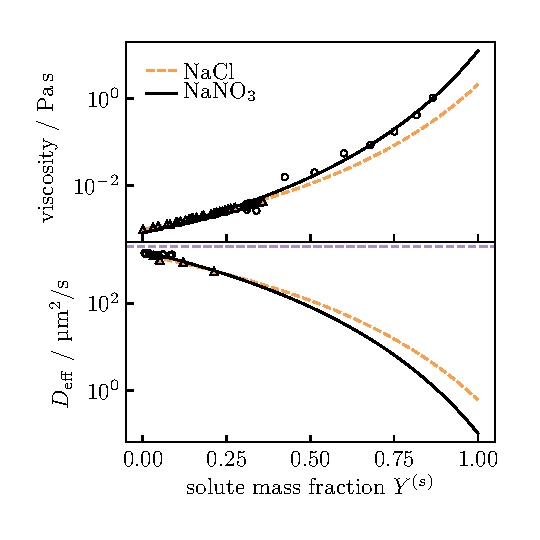
\includegraphics[width=0.9\linewidth,outer]{aerosol-diffusion-fit}
  \caption[Viscosity and diffusion coefficients of aqueous ionic solutions]{
    Numerical fits of binary diffusion coefficients for aqueous ionic solutions.
    a) fits of viscosity to an Arrhenius-like form \eqref{eq:vft-fit} to experimental values \cite{PowerCS2013,BaldelliAST2016}.
    b) diffusion coefficient from the viscosity fits assuming a Stokes-Einstein form \eqref{eq:stokes-einstein}, where the Stokes radius is obtained by calibration with direct measurements of diffusion at \SI{300}{\kelvin} for \ce{NaCl} \cite{LyubartsevJPC1996} and \SI{25}{\celsius} for \ce{NaNO3} \cite{YehJCED1970}.
    The dashed-purple horizontal line shows the diffusion constant of pure \ce{H2O} for reference, to be distinguished from the binary diffusion constants in the limit $Y^{(s)} \to 0$.}
  \label{fig:diffusion-fit}
\end{SCfigure}

We employ two simplifications in our calculations concerning the effects of droplet temperature.
First, our volume additivity assumption \eqref{eq:volume-additivity} makes the density temperature independent; this neglects conduction forces caused by temperature gradients and results in more heterogeneous droplets.
%In reality temperature gradients will be present in a drying droplet from evaporative cooling, so conductive forces will help keep the solution well-mixed; we will thus overestimate the inhomogeneities of the concentration profile.
Secondly, we approximate $T \sim T_\infty$ in the Stokes-Einstein relation \eqref{eq:stokes-einstein}
This approximation neglects evaporative cooling which would slow diffusion, so overestimates the diffusion constant and will result in more heterogeneous droplets.
It is unclear \emph{a priori} which of these opposing effects dominates.
Note: later we model the droplet temperature $T$ explicitly for treating solvent evaporation and nucleation rates, but we have not incorporated this temperature into the diffusion constant.

\subsection{Droplet boundary conditions}

Initially the droplets are prepared in equilibrium, so they are well-mixed solutions and we can assume a uniform initial concentration profile.
At $t=0$ the humidity is reduced leading to evaporation of the solvent.
The evaporation rate determines the boundary conditions for the diffusion equation \eqref{eq:final-diffusion}.

Integrating the species continuity equation \eqref{eq:species-continuity} gives the total mass flow into the droplet (of each species) as
\begin{equation}\label{eq:integral-continuity}
  \frac{d m^{(i)}}{dt} =
  \int_{V(t)} \frac{\partial \rho^{(i)}}{\partial t} \, d V +
  \int_{\partial V(t)} \rho^{(i)} \, \vec{v}_{\partial V(t)} \cdot d\vec{S}
%  \qquad i \in \{f,s\}
\end{equation}
where $V(t)$ is the volume of the droplet at time $t$ and $\vec{v}_{\partial V(t)}$ is the velocity of the boundary, and the vectorial surface element $d\vec{S}$ points in the direction of the outer normal vector.
We assume the solute does not leave the droplet, so all mass flow at the boundary must be due to the solvent.
Inserting the diffusion equation \eqref{eq:final-diffusion} into \eqref{eq:integral-continuity} and applying Stokes' theorem gives
\begin{equation}
  \frac{d m^{(s)}}{dt}
  =
  \int_{\partial V(t)}
  \Big(
  \rho^{(i)} \vec{v}_{\partial V(t)} +
  D_\mathrm{eff} \vec{\nabla} \rho^{(s)}
  \Big)
  \cdot d\vec{S}
  = 0.
\end{equation}
For spherical droplets this gives the boundary condition
%% \begin{equation}
%%   \frac{d m^{(s)}}{dt}
%%   =
%%   4 \pi R^2
%%   \rho^{(s)}(R) \left(
%%   \frac{dR}{dt}
%%   + \frac{D_\mathrm{eff}}{\rho^{(s)}} \frac{\partial \rho^{(s)}}{\partial r}
%%   \right)
%% \end{equation}
%% so
\begin{equation}
  \left. \frac{\partial \rho^{(s)}}{\partial r} \right|_{r=R(t)}
  =
  -
  \frac{\rho^{(s)}}{D_\mathrm{eff}(R)}
  \frac{dR}{dt}.
\end{equation}
Assuming volume additivity \eqref{eq:volume-additivity} we can determine the radial evolution from mass conservation as
\begin{equation}\label{eq:radial-evolution}
  \frac{dR}{dt}
  =
  \frac{\dot{m}}{4\pi R^2 \rho^{(f)}_0}
\end{equation}
so we need a model of the evaporation rate $\dot{m} := \tfrac{dm^{(f)}}{dt}$ to close this system of equations.

We now derive the classical result for quasistatic droplet vaporisation, loosely following the exposition of standard texts e.g.\ Refs.\ \cite{Slattery1999, Sirignano2010}.
Relaxation in the vapour phase occurs much faster than inside the liquid droplet, so we can assume that the flows in the vapour phase are quasi-steady.
The time-derivative in the continuity equations \eqref{eq:species-continuity} and \eqref{eq:species-continuity-relative} thus vanishes leaving
\begin{subequations}
  \begin{align}
    \vec{\nabla} \cdot (\rho \vec{v})
    &=
    0
    \\
    \vec{\nabla} \cdot (\rho^{(i)} \vec{v}^{(i)})
    =
    \vec{\nabla} \cdot (\rho^{(i)} \vec{v} + \vec{j}^{(i)})
    &=
    0
    \qquad i \in \{f,g\}
    %% \frac{1}{r^2} \frac{d}{dr} \left(
    %% r^2 \rho u Y_i - r^2 D_V \frac{d(\rho Y_i)}{dr}
    %% \right)
  \end{align}
\end{subequations}
with the total mass continuity equation obtained by summing over both species in \eqref{eq:species-continuity} and using $\sum_i \rho^{(i)} = \rho$.
Assuming spherical symmetry we find that total mass conservation obeys
\begin{equation}\label{eq:vapour-mass-conservation}
  r ^2 \rho v
  =
  \textrm{constant}
  =
  -\frac{\dot{m}}{4\pi}
\end{equation}
with radial speeds $v = |\vec{v}|$ and $v^{(i)} = |\vec{v}^{(i)}|$.
Similarly, for the evaporating component we obtain the ordinary differential equation
\begin{equation*}\label{eq:quasistatic-vapour-species-conservation}
  r^2 \rho v Y^{(f)} - r^2 \rho D_v \frac{d Y^{(f)}}{dr}
  =
  -\frac{\dot{m}}{4\pi}
\end{equation*}
where we assumed Fickian diffusion for the relative flux term with $D_v$ as the effective binary diffusion constant for the vapour.
Using total mass conservation \eqref{eq:vapour-mass-conservation} we can rewrite this as
\begin{equation}\label{eq:vapour-ode}
  \frac{d Q}{dr} (Y^{(f)} - 1)
  - \frac{d (Y^{(f)} - 1)}{dr}
  = 0
\end{equation}
with
\begin{equation}\label{eq:vapour-ode-integration-factor}
  Q(r)
  =
  \frac{\dot{m}}{4\pi}
  \int_r^\infty  \frac{1}{\rho D_v (r')^2} \, dr'.
\end{equation}
Upon integration%
\marginfootnote{One way of doing this is to multiply through by the integrating factor $e^{-Q(r)}$.}
we find
\begin{equation*}
  (Y^{(f)}(r) - 1) e^{-Q(r)}
  =
  \textrm{constant}.
\end{equation*}
or
\begin{equation*}
  \frac{1 - Y^{(f)}(R^+)}{\displaystyle{1 - \lim_{r \to \infty}} Y^{(f)}(r)}
  =
  1 + B
  =
  e^{Q(R)}
\end{equation*}
where the superscript in $Y^{(f)}(R^+)$ indicates the mass fraction of the solvent component is taken on the vapour side of the boundary and we have defined the \emph{Spalding number} as
\begin{equation}\label{eq:spalding-number}
  B
  =
  \frac{
    \displaystyle{\lim_{r \to \infty}} Y^{(f)}(r) - Y^{(f)}(R^+)
  }{
    1 - \displaystyle{\lim_{r \to \infty}} Y^{(f)}(r)
  }.
\end{equation}
Upon reinserting the definition of $Q(r)$ \eqref{eq:vapour-ode-integration-factor} and rearranging we obtain 
\begin{equation*}
  \frac{dm^{(f)}}{dt}
  =
  \frac{
    4\pi \ln{(1 + B)}
  }{
    \int_r^\infty  \frac{1}{\rho D_v (r')^2} \, dr'
  }.
\end{equation*}
If we take $\rho = \rho_v$ and $D_v$ as constants in the vapour phase, then we obtain the classical result for quasistatic vaporisation as \cite{Slattery1999,Sirignano2010}
\begin{equation}\label{eq:quasistatic-vaporisation}
  \frac{dm^{(f)}}{dt}
  =
  4\pi \rho_v D_v R \ln{(1 + B)}.
\end{equation}
Matching the partial pressures of the solvent on either side of the boundary through the Clausius-Clapeyron relation gives% the molar fraction
\begin{equation}\label{eq:molar-fraction}
  %X^{(f)}(R^+) =
  %a_w \frac{p_{eq}}{p}
  p_f(R^+)
  =
  p_f(R^-)
  \exp{\left( \frac{L}{R} \frac{T - T_\infty}{T T_\infty} \right)}
\end{equation}
where $p_f(R^\pm)$ are the partial pressures on either side of the surface which we can convert to mass fractions assuming Raoult's law in the gas phase combined with experimental fits of the solvent activity \cite{CleggJPCA1998}.
%The mass fraction $Y^{(f)}(R^+)$ can then be obtained from $X^{(f)}(R^+)$.
%% Neglecting the effects of radiative heat transfer, the steady state heat flux through the droplet boundary in the steady state is \cite{KulmalaJAS1992,RovelliJPCA2016}
%% \begin{equation}
%%   \dot{Q}
%%   =
%%   %Q_R
%%   - h \frac{dm^{(f)}}{dt} + 4\pi R K (T - T_\infty)
%% \end{equation}
%% %where $Q_R$ is the excess heat flux of radiation over absorption,
%% where $h_v$ is the vapour enthalpy of the evaporating solvent, and $K$ is the thermal conductivity of the gas phase.
Finally, assuming a steady state heat flux through the boundary, and neglecting the radiative heat transfer and the droplet heat capacity, gives the temperature difference between the droplet surface and the ambient temperature as \cite{KulmalaJAS1992,RovelliJPCA2016}
\begin{equation}\label{eq:temperature-difference}
  T - T_\infty = \frac{L}{4\pi R K} \frac{dm^{(f)}}{dt}
\end{equation}
% $L = h_v - h_l$
where $L$ is the specific latent heat of vaporisation, and $K$ is the thermal conductivity of the vapour phase.
Together, equations \eqref{eq:quasistatic-vaporisation}, \eqref{eq:spalding-number}, \eqref{eq:molar-fraction} and \eqref{eq:temperature-difference} form a complete set of equations that can be solved (numerically) to obtain the evaporation rate.

Typically the classic vaporisation rate equation \eqref{eq:quasistatic-vaporisation} requires semi-empirical corrections to treat more complex mass and heat transport phenomena at the boundary.
We introduce the \emph{Sherwood number} $\sherwood$ to correct the vaporisation rate giving
\begin{equation}\label{eq:sherwood-correction}
  \frac{dm^{(f)}}{dt}
  =
  2\pi \, \sherwood \, \rho_v D_v R \ln{(1 + B)}.
\end{equation}
As a simplification we approximate $\sherwood$ as a constant throughout the droplet's trajectory and determine it by fitting the initial value of $\tfrac{dR}{dt}$ to the experiments.
At constant vaporisation rate the solution to the radial evolution equation \eqref{eq:radial-evolution} yields
\begin{equation}
  R(t)^2
  =
  R(t=0)^2
  + \left(2R \, \frac{dR}{dt}\right)_{t=0} t,
\end{equation}
valid at short times.
Fitting the early part of the experimental trajectory gives the initial $\tfrac{dR}{dt}$ and thus $\sherwood$ through \eqref{eq:sherwood-correction}.

\subsection{Implementation and results}

\begin{SCfigure}
  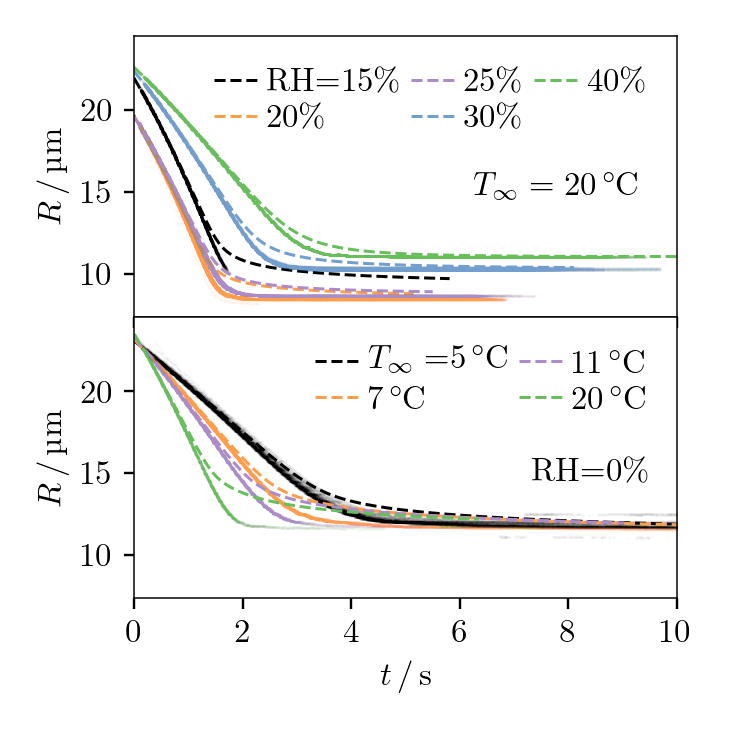
\includegraphics[width=0.9\linewidth,outer]{nano3-trajectory}
  \caption[Evolution of drying droplet radii]{
    Evolution of \ce{NaNO3} aerosol droplet radii from the numerical model (dashed lines) and experiments shown by points with 1\% transparency, showing reasonable agreement at short times until longer times when the evaporation rate is underestimated.
    a) varying relative humidity while ambient temperature is kept fixed, for an initial solute mass fraction of $Y^{(s)} = 0.125$.
    b) varying ambient temperature while relative humidity is kept fixed, for an initial solute mass fraction of $Y^{(s)} = 0.2$.}
  \label{fig:nano3-trajectory}
\end{SCfigure}

We discretise the solute concentration profile $\rho^{(s)}(r)$ onto a uniformly spaced grid over $r \in [0, R(t)]$.
To handle the moving boundary it is convenient to work in the rescaled coordinate $\tilde{r} = \frac{r}{R(t)} \in [0, 1]$.
For the discretisation we define the vector $\vec{\rho} := \{\rho_0, \rho_1, \cdots, \rho_N\}$ where $\rho_i := \rho^{(s)}\left(\tilde{r} = \frac{i}{N}\right)$.
The complete history of the evolution of the droplet then involves both $\vec{\rho}$ and $R$ variables.
In addition, it is convenient to introduce $\dot{R}$ as its own variable so that the final Jacobian for the diffusion equation \eqref{eq:final-diffusion} has tridiagonal form.
This gives us the evolving droplet state variable $\vec{x} = (\vec{\rho}, R, \dot{R})$.

To integrate a timestep $\Delta t$ we use the Crank-Nicolson \cite{CrankMPCPS1947} method where
\begin{equation*}
  \frac{\vec{x}(t + \Delta t) - \vec{x}(t)}{\Delta t}
  =
  \frac{1}{2}
  \left(
  \left. \frac{\partial \vec{x}}{\partial t} \right|_{t + \Delta t}
  +
  \left. \frac{\partial \vec{x}}{\partial t} \right|_t
  \right)
  + \mathcal{O}(\Delta t^2).
\end{equation*}
As the evolution equations are nonlinear this must be solved iteratively to find a self-consistent solution.
Introducing the $k$th approximation for $\vec{x}(t + \Delta t)$ as $\vec{x}^{(k)}(t + \Delta t)$, we write the next term in the sequence as $\vec{x}^{(k+1)} = \vec{x}^{(k)} + \delta \vec{x}^{(k)}$
We obtain
\begin{equation*}
  \frac{\vec{x}_{n+1}^{(k)} + \delta\vec{x}_{n+1}^{(k)} - \vec{x}_n}{\Delta t}
  =
  \frac{1}{2}
  \left(
  \frac{\partial (\vec{x}_{n+1}^{(k)} + \delta\vec{x}_{n+1}^{(k)})}{\partial t}
  +
  \frac{\partial \vec{x}_n}{\partial t}
  \right)
\end{equation*}
using the subscript $n$ as shorthand for the time.
This is a matrix equation that can be inverted for $\delta \vec{x}^{(k)}$.
Convergence is deemed to occur where $\delta \vec{x}^{(k)}$ falls below some threshold value.
The main advantage of this scheme over more simple schemes (e.g. forward Euler method where just the initial $\frac{\partial \vec{x}_n}{\partial t}$ is taken) is that the error is of order $\Delta t^2$ ensuring rapid convergence with small timesteps.

We integrated initially homogeneous droplets of \ce{NaCl} and \ce{NaNO3} for various ambient conditions.
The resulting radius , illustrated for \ce{NaNO3} in Fig.\ \ref{fig:nano3-trajectory}; we see that at short times there is excellent agreement, but the evaporation rate is underestimated at longer times.
This is likely do to limitations of the simplified evaporation model \eqref{eq:sherwood-correction} or because the neglect of conductive forces causes the evaporation to become diffusion-limited at long-times when the surface is highly enriched.
We achieve good agreement with experiments for \ce{NaCl} across their entire time-evolution (Fig.\ \ref{fig:nacl-trajectory}(b)) because these droplets crystallise before the slowdown of the evaporation rate.

\section{Nucleation model}
\label{sec:nucleation}

\subsection{Droplet nucleation rates}

\begin{SCfigure}
  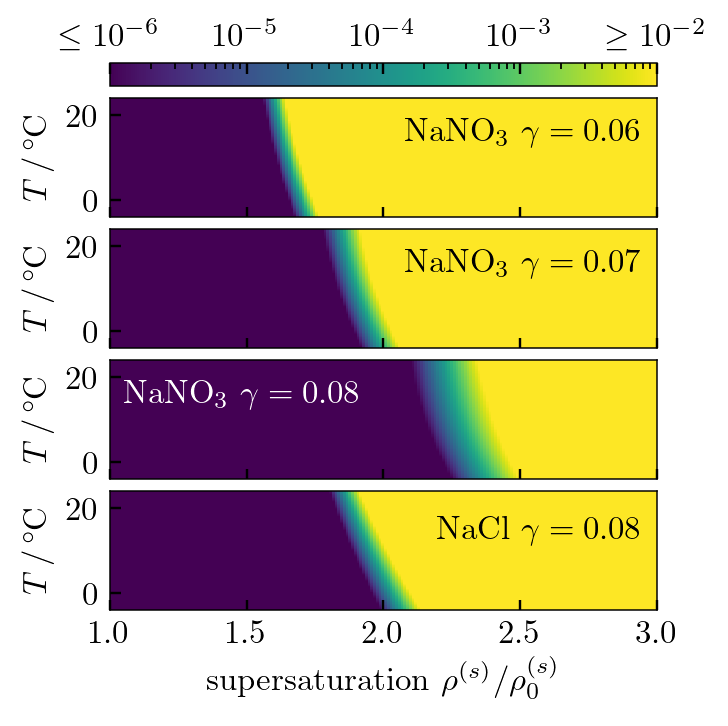
\includegraphics[width=0.9\linewidth,outer]{aerosol-cnt}
  \caption[Nucleation rates predicted by classical nucleation theory]{
    Shell nucleation rate $J\xi$ (\si{\per\micro\metre\squared\per\second}) predicted by classical nucleation theory for aqueous \ce{NaNO3} and \ce{NaCl} solutions at different state points.
    The dark blue and bright yellow regions show where nucleation is essentially impossible or instantaneous on the experimental timescale.
    Different estimates of solid-liquid surface tension $\gamma$ (given in \si{\newton\per\metre}) do not result in a different qualitative picture: a nucleation rate which monotonically increases with supersaturation and temperature.}
  \label{fig:cnt}
\end{SCfigure}

Denoting the rate of solute nucleation per unit volume as $J$, the continuum limit nucleation rate for the entire droplet is
\begin{equation}\label{eq:droplet-nucleation-rate}
  W
  =
  \int_V J dV
  =
  4\pi \int_0^R J(r) \, r^2 dr.
\end{equation}
Both the local $J$ and total rates $W$ contain an implciit time dependence because of their dependency on the evolving variables $R$, $\rho^{(s)}$ and $T$.
For homogeneous nucleation $J$ depends solely on the state variables $\rho^{(s)}$ and $T$.
Nucleation rates are typically strongly concentration dependent \cite{ValerianiJCP2005,DesarnaudJPCL2014,SearJPCM2007}, so we anticipate nucleation to occur at the boundary $r=R(t)$ where the solute concentration is greatest.
Allowing for heterogeneous nucleation $J$ could acquire an additional dependence on the inhomogeneities in the system; as the experiments were performed with high-purity precursor compounds to mitigate the effect of chemical impurities, we expect the main potential site for heterogeneous nucleation to be the liquid-air interface.
Whichever nucleation mechanism dominates, we expect it to occur at the boundary so the total rate \eqref{eq:boundary-nucleation-rate} reduces to
\begin{equation}\label{eq:boundary-nucleation-rate}
  W
  \sim
  4\pi R^2 J \xi
\end{equation}
where $J$ is now evaluated at the boundary, and we introduced $\xi$ as the thickness of the typical shell region over which nucleation occurs.
We will give nucleation rates in terms of $J \xi$, assuming a value $\xi = \SI{1}{\micro\metre}$ to set the absolute scale of the rates predicted by theory (section \ref{sec:cnt}) to most closely match the experiments.

We can relate the nucleation rates to the experimentally observed events by assuming Poisson statistics.
We define the survival probability as
\begin{equation*}
  p_\mathrm{liq}(t)
  :=
  \textrm{Prob}\left[ \textrm{no nucleation by time } t \right],
\end{equation*}
The mean number of nucleation events in the time interval $\Delta t$ is simply $W \Delta t$, giving the probability that there is no nucleation event after a time $\Delta t$ as
\begin{equation*}
  p_\mathrm{liq}(t + \Delta t) = p_\mathrm{liq}(t) e^{-W \Delta t}.
\end{equation*}
Taking the infinitesimal limit and using the fact that droplets are prepared in the liquid state giving the initial condition $p_\mathrm{liq}(t=0) = 1$ yields
\begin{equation}\label{eq:survival}
  p_\mathrm{liq}(t)
  =
  \exp{\left( -\int_0^t W \, dt \right)}.
\end{equation}
As we have already determined the droplet's radius and concentration profile from the evolution equations described in section\ \ref{sec:evolution}, we are left needing a model for the nucleation rate per unit volume $J$ before we can determine $p_\mathrm{liq}$.

\subsection{Nucleation models}
\label{sec:cnt}

%From \eqref{eq:cnt-barrier} we expect a homogeneous nucleation rate per unit volume as
For nucleation processes with a single barrier the rate per unit volume goes as
\begin{equation}\label{eq:nucleation-rate-barrier}
  J = \kappa \exp{\left(-\frac{\Delta G^{*}}{k_B T}\right)}
\end{equation}
where $\kappa$ is a kinetic prefactor and $\Delta G^*$ is thermodynamic barrier for the process.
A widely used approximation for the kinetic prefactor is \cite{SearJPCM2007}:
\begin{equation}
  \kappa = n_I j Z
\end{equation}
$n_I$ is the number density of potential nucleation sites, $j$ is the rate of aggregation to these sites, and $Z$ is the Zeldovich factor.
These last two quantities are typically further approximated as \cite{SearJPCM2007}
\begin{subequations}
  \begin{align}
    j &\sim n D_\mathrm{eff} R^* \\
    Z &\sim (N^*)^{-\tfrac{2}{3}}
  \end{align}
\end{subequations}
where $n$ is the solute number density, $N^*$ is excess number of molecules in the critical nucleus and $R^*$ is its radius.
The barrier $\Delta G^*$ depends on the specific nucleation mechanism.

For homogeneous nucleation the sites of nucleation are simply the solute molecules themselves so $n_I = n$.
The driving force for the transition is the chemical potential change $\Delta \mu$ from formation of the new phase.
In classical nucleation theory (CNT) the surface tension between the crystal and liquid is imagined as the main obstacle to nucleation.
Combining the two contributions leads to the barrier
\begin{equation}
  \Delta G = \gamma A - |\Delta \mu| n_c V
\end{equation}
where $n_c$ is the crystal number density, and $A, V$ are the surface areas and volumes of the nucleated region.
The thermodynamic barrier to nucleation is then the maximum of this formula; assuming a perfectly spherical crystal seed this gives
\begin{align}\label{eq:cnt-barrier}
  \Delta G^{*} &= \frac{4}{3} \pi (R^{*})^2 \gamma \\
  (R^{*}) &= \frac{2\gamma}{n_c |\Delta\mu|}.
\end{align}
The chemical potential expressed in terms of mean ionic activity is\cite{DesarnaudJPCL2014}
\begin{equation}
  %\exp{\left(
  \frac{\Delta \mu}{k_B T}
  %\right)}
  =
  2 \ln{\left( \frac{a_\pm}{a_{0\pm}} \frac{\rho^{(s)}}{\rho^{(s)}_0} \right)}
\end{equation}
where $a_\pm$ is mean ionic activity coefficient, $a_0$ is its value at saturation and $\rho^{(s)}_0$ is the threshold saturation concentration.

We find that CNT predicts homogeneous nucleation rates which increase monotonically in both concentration and temperature.
In Fig.\ \ref{fig:cnt} we show the predicted rates for \ce{NaCl} with $\gamma=\SI{0.08}{\newton\per\metre}$ and \ce{NaNO3} with different estimates of surface tension; we find that the rates increase so rapidly with concentration that they are essentially a step function over the timescale of the experiments.
This is qualitatively correct for \ce{NaCl}, so we are able to accurately predict the time of nucleation in the experiments shown in Fig.\ \ref{fig:nacl-trajectory}.
By contrast, the experiments show that the final survival probability for \ce{NaNO3} droplets is often in the range $0 < p_\mathrm{liq} < 1$ which is not consistent with nucleation rates being characterised by a step function, which we will make more quantitative in the next section.

\begin{SCfigure}
  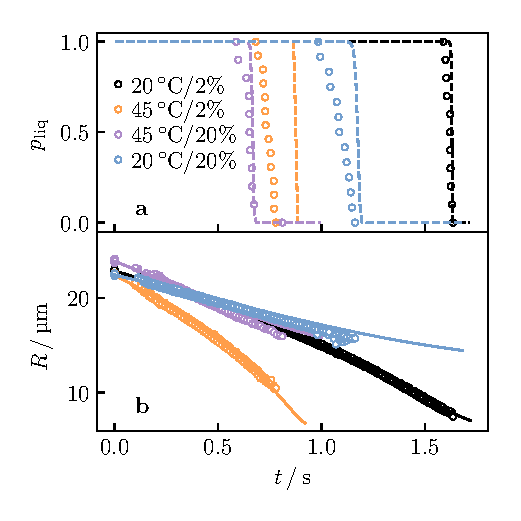
\includegraphics[width=0.9\linewidth,outer]{nacl-trajectory}
  \caption[Evolution of \ce{NaCl} droplets: theory and experiments]{
    Evolution of \ce{NaCl} droplets in dry air $\mathrm{RH}=0\%$ from experiments (points) and the numerical model (lines) for different ambient temperatures and initial solute mass fractions.
    a) the probability that a droplet survives without nucleating, assuming the liquid-crystal surface tension $\gamma = \SI{0.08}{\newton\per\metre}$ \cite{DesarnaudJPCL2014} for the numerical model.
    b) the evolution of droplet radius showing good treatment of solvent evaporation rates.
  }
  \label{fig:nacl-trajectory}
\end{SCfigure}

\subsection{Inferring nucleation rates from experiments}

We can try to determine the nucleation rates directly from experiments by observing the stochastic nucleation behaviour over repeat trajectories and comparing these against the numerical model.
The experiments give us the true survival probabilities $p_\mathrm{liq}$ of which we can determine the droplet nucleation rate $W$ exactly by numerical differentiation.
Combined with the numerical model, which gives us the precise state of the droplet, we can infer $J\xi$ from inversion of the rate formula \eqref{eq:boundary-nucleation-rate} under the assumption that nucleation is boundary-dominated.
%% We can make some progress by making some strong assumptions about the form of $J \xi$ based on physical intuition.
%% We will then test for self-consistency to justify this approach in an ad-hoc manner.

Differentiation of the survival probability \eqref{eq:survival} yields
\begin{equation}
  \dot{p}_\mathrm{liq}
  =
  - W p_\mathrm{liq},
\end{equation}
upon combining this with our assumption that nucleation occurs near the boundary \eqref{eq:boundary-nucleation-rate} allows to write the nucleation rate as
\begin{equation}
  J\xi
  =
  - \frac{1}{4\pi R^2} \frac{\dot{p}_\mathrm{liq}}{p_\mathrm{liq}}
\end{equation}
which we can determine from the experimentally observed $p_\mathrm{liq}$ trajectory.
The derivative of $p_\mathrm{liq}$ can be obtained through fitting.
The survival probabilities decay monotonically as a generalised step function, so we fit the experimental trajectories with the Fermi-Dirac form
\begin{equation}
  p_\mathrm{liq}(t) - \lim_{t \to \infty} p_\mathrm{liq}(t)
  =
  \frac{1 - \lim_{t \to \infty} p_\mathrm{liq}(t)}{\exp{\left[\epsilon(t - t_s)\right]} + 1}
\end{equation}
where $t_s$ is the time at which saturation is reached $\rho^{(s)}(R) = \rho^{(s)}_0$, and introducing the fitting function
\begin{equation*}
  \epsilon(t)
  =
  \begin{cases}
    at + bt^2 - c / t & \; t > 0 \\
    - \infty & \; t < 0
  \end{cases}
\end{equation*}
subject to the constraint that the fitting parameters $a, b, c \in [0, \infty]$ to ensure that $p_\mathrm{liq}$ decreases monotonically from $p_\mathrm{liq}(t=0)=1$.

We perform this inversion procedure for the \ce{NaNO3} droplets in Fig.\ \ref{fig:state-points}(b).
The resulting nucleation rates show non-mononic behaviour, increasing to a maximum before decreasing to essentially zero over the duration of the experiment.
This results in a finite final survival probability $p_\mathrm{liq} > 0$, and starkly contrasts with the picture predicted by CNT where $p_\mathrm{liq}$ would remain close to unity for most of the experiment before sharply dropping to zero as all droplets reproducibly crystallise.

\begin{SCfigure}
  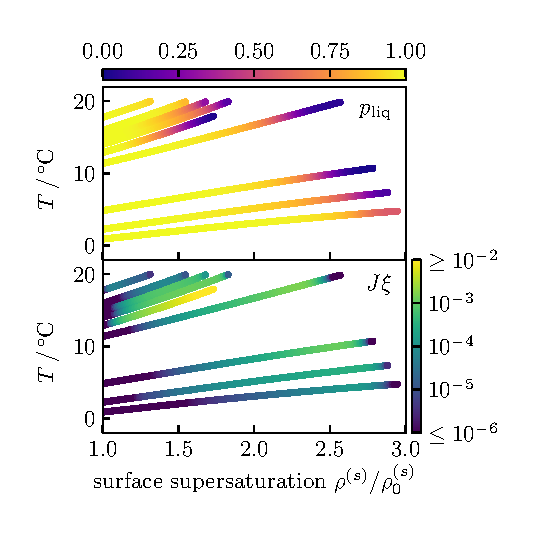
\includegraphics[width=0.9\linewidth,outer]{nano3-nucleation-rates}
  \caption[Experimentally observed nucleation rates in \ce{NaNO3} droplets]{
    State points explored by experiments with drying \ce{NaNO3}--\ce{H2O} aerosol droplets as determined from our numerical model for 9 datasets for different initial conditions.
    a) the survival probability in the experiments (i.e.\ the probability that a droplet has not crystallised), with state-point inferred from the model.
    b) the corresponding nucleation rates assuming boundary-dominated nucleation \eqref{eq:boundary-nucleation-rate} showing non-monotonic behaviour in increased concentration and temperature in contrast with the predictions of classical nucleation theory in Fig.\ \ref{fig:cnt}.}
  \label{fig:state-points}
\end{SCfigure}

\section{Conclusions}

We have developed a numerical model based on a diffusion equation with an extrapolation of the diffusion constant to high concentrations assuming the Stokes-Einstein relation.
The resulting droplet evolution conforms well to the experimental trajectories.
Assuming boundary dominated nucleation we are able to predict nucleation rates inside the droplet, and extract nucleation rates at differing state points from the experimental trajectories.

We found that CNT works well for predicting crystal nucleation in \ce{NaCl} but not \ce{NaNO3} aerosols.
In both cases CNT predicts nucleation essentially after a threshold surface saturation is reached, whereas experiments show nucleation in \ce{NaNO3} has stochastic behaviour.
This emerges from the fact that nucleation rates predicted by CNT monotonically increase in concentration and temperature.
In particular, the change in nucleation rate from increased concentration is so dramatic that the behaviour of CNT is essentially unchanged by small adjustments to the model parameters.

CNT is a model for homogeneous nucleation, so it is possible that it fails because crystallisation occurs for \ce{NaNO3} through heterogeneous nucleation.
The same stochastic phenomena are observed when repeating the experiments with the same droplet on a cycle of decreasing and increasing the RH to dry and melt the droplet; this rules out heterogeneous nucleation through impurities, as the chemical makeup is the same in each cycle yet the phenomenon persists.
This leaves the gas-liquid phase boundary itself as a site for hetereogeneous nucleation.

It is highly likely that the model overestimates the surface enrichment because at long times the simulated evaporation rates become limited by solute diffusion at the boundary.
The diffusion limit would persist even if more sophisticated transport phenomena were introduced to the evaporation model.
Surface enrichment is overestimated because we have neglected the effect of temperature gradients inside the droplet, and because we have used an extrapolation of low concentration diffusion data which likely to underestimate diffusion at high concentrations.
Temperature gradients create inward convection currents reducing surface enrichment.
Our extrapolation of the diffusion constant assumed the Stokes-Einstein relation holds across the whole state space, however this relation can be violated at high viscosities \cite{BerthierRMP2011}.
The rapid increase of viscosity with salt concentration in our model leads to a feedback loop where diffusion becomes increasingly difficult as the surface is enriched.
Correcting for these effects, we expect the surface concentrations explored by the experiments to increase to a maximum before decreasing which could explain non-monoticity.
However, this can only partially explain the observed behaviour because CNT is extremely sensitive to concentration.

%Our evaporation model considerably simplifies the transport phenomena at the phase boundary, though it becomes limited by the rate of solute diffusion at the boundary at long times suggesting that we are underestimating the rate of mixing.

%It is possible that our assumption that kinetics occurs purely through Fickian diffusion oversaturates the solute at the boundary, complicating our analysis of the nucleation rate.
%To go beyond this one would have to model temperature gradients to allow for conduction forces which help keep the droplet well-mixed.

This work is important in showing that the nucleation rate of nitrate aerosol is not only influenced by the level of supersaturation, but also by the drying kinetics itself because of an interplay between the inhomogeneity of the concentration profile and droplet temperature.
This is important for climate predictions where an understanding of the phase of atmospheric aerosol is crucial, and also valuable for spray-drying models where control over the resulting phase could be enabled by tuning the various drying parameters.

%% It is unlikely to be due to the trajectories being incorrect: even varying the most poorly estimated parameter for \ce{NaNO3}, the surface tension, does not change the CNT prediction.
%% Because of the sensitivity of CNT on parameters, it would require a remarkable degree of fine tuning to fit CNT model with any physically plausible parameters.
%% It's possible nucleation of \ce{NaNO3} occurs via a more complex kinetic pathway, e.g.\ multiple steps \cite{?,?,?}.
%% Alternatively, the experimental nucleation could be occurring via heterogeneous nucleation (e.g.\ impurities in the sample).
%% This is unlikely however, as the experiments can maintain the same salt sample and follow the single trajectory and it will still show the same stochastic behaviour.
%% Impurities are not likely to be in the solvent, or we would likely see the same phenomenon in \ce{NaNO3} nucleation.

%An option would be to relax the assumption that the temperature of the droplet is constant, as convection effects could play a key role in mixing the solution.
%Solving the Navier-Stokes equations would be essentially exact, though expensive route to include this.
%Less expensive would be to use vortex models or effective-conduction models which treat the internal circulation/convection of heat in an ad hoc manner.

\ifdefined\includebibliography
  \printbibliography
\fi

\end{document}

%TC: macro \marginfootnote [other]
%TC: envir SCfigure [] other
%TC: macrocount beginSCfigure [figure]
\documentclass[11pt,twoside]{report}
\usepackage{preamble}
\setcounter{chapter}{7}
\graphicspath{{../img/}}
\def\includebibliography{}

\externaldocument{background}
\externaldocument{supercooled-liquids}
\externaldocument{morphometric-framework}
\externaldocument{morphometric-applications}
\externaldocument{resummation}
\externaldocument{aerosols}

\begin{document}
\chapter{Conclusion}
\epigraph{We demand rigidly defined areas of doubt and uncertainty!}{Douglas Adams, \emph{The Hitchhiker's Guide to the Galaxy}, (1979).}

At high densities, the dynamical properties of supercooled liquids show marked complexity distinguishing them from their ordinary counterparts at lower densities.
We have attempted to develop methods to better understand the nature of dynamical arrest and the glass transition, and nucleation of crystals within the metastable liquid.
Most of this work has focused on the first question, so we will emphasise that topic here and return to nucleation towards the end.

%with hard spheres as the model system, and to address nucleation of the crystals in a real system.
%Specifically, supercooled liquids and the glass transition, and nucleation of the crystal.

Liquids approaching their glass transition display a dramatic slowdown in their relaxation behaviour, while showing no obvious structural change at the level of pair correlations.
In chapter \ref{chapter:glass} we summarised the various scenarios posited to explain this phenomenon, highlighting the potential role of amorphous order in mean-field theories and structural order in geometric theories.
These thermodynamic scenarios in particular posit solely static mechanisms for dynamic arrest, which we argued could be detected through the many-body correlation functions.
Developing from this observation, in chapter \ref{chapter:morphometric-framework} we showed that the correlation functions could be expressed in terms of a potential of mean force, itself dependent on the interaction potential and a chemical potential term.
The key approximation we employed was the \emph{morphometric approach}, where the chemical potential is expressed as an expansion in size measures: the volume, surface area and integrated curvature measures.
Using the many-body correlation functions we attempted to explore the energy landscape of local structures in chapter \ref{chapter:morphometric-applications}, to look for features which could be connected with dynamical arrest.

%Disappointingly we have few results.

We have presented three justifications of the morphometric approach for hard particle systems.
First, we derived it in the usual way as a limit of fundamental measure theory (section \ref{sec:fmt}).
Second, we argued for the morphometric \emph{ansatz} as the natural generalisation of scaled particle theory (chapter \ref{chapter:morphometric-framework}); furthermore, we used integral geometry to argue that this \emph{ansatz} generalises the form of an extensive quantity (section \ref{sec:generalised-intrinsic-volumes-d}).
And last, we derived the morphometric form for the chemical potential by resumming a component of the virial series (chapter \ref{chapter:resummation}).

The latter two justifications are in principle new arguments, though we suspect neither will be of any surprise to the liquid state community; in some sense, these routes are all equivalent because they fundamentally reduce to integral geometric arguments.
%, and properties of the intrinsic volumes.
The primary advancements of this work have thus been technological, rather than fundamental, in nature.
In particular, we introduced the trick of imposing self-consistency of the virial theorem to derive a new set of morphometric coefficients in hard spheres (chapter \ref{chapter:morphometric-framework}).
These coefficients yield a theory for chemical potentials capable of producing highly accurate correlation functions, even at high densities.
Although we have made some modest contributions to treating local structure in chapter \ref{chapter:morphometric-applications} (described below), fundamentally the accuracy of all subsequent results depended on application of this trick.

In chapter \ref{chapter:morphometric-applications} we introduced methods to extend the formalism of energy landscapes, normally applied to soft potentials, to local structures of hard spheres; many adaptations were required to handle the singularity of the hard sphere interaction potential.
%Concerning morphometric approach: most of the developments have been in methods.
We explored a method of predicting the concentrations of structural motifs within the liquid, and developed a route to do similar calculations along saddles
%\marginfootnote{These calculations used techniques from Bayesian inference which were a late addition to this thesis, and are subsequently the least well-explained.
%  Their inclusion provides a route to extending calculations to dynamical phenomena, so I felt it important to include them for a more complete perspective of available options.}
for connecting with dynamics.
Notably, we found a bimodality in the distribution of energy states corresponding to distinct structural symmetries, of potential importance to structural viewpoints of dynamical arrest.
This work lays the groundwork for a quantitative assessment of the landscape properties of local regions within the liquid, which could explore the validity of random first-order transition and related theories.

There are two limits to the accuracy of the morphometric approach: the thermodynamic coefficients entering the theory, and the limitations \emph{ansatz} itself.
We found that improving the coefficients was enough to obtain accurate results in chapters \ref{chapter:morphometric-framework} and \ref{chapter:morphometric-applications}, though the theory was not exact and so there is room for improvement particularly at high densities.
We attempted to provide some insight into the theory behind the morphometric approach in chapter \ref{chapter:resummation}, with a view to potentially supplementing the \emph{ansatz} with additional terms.
There, we found a contribution to the chemical potential which is rigorously of morphometric form, the thermodynamic coefficients of which capture most of the bulk free energy in hard spheres up to moderate densities; this observation potentially explains why the approach works well in the first place.
Furthermore, the resulting theory applies to arbitrary mixtures of hard convex particles without modification of the morphometric \emph{ansatz}, suggesting that extensions to other hard particle systems are possible.

%% Generalisations:
%% Hard particle extension is done.
%% We tested the theory up to mode-coupling, finding it accurate.
%% Polydisperse ready to go: direct comparison with the high density swap data could be made.
%% Could be a challenge to do the virial route coefficients, 
%% By introducing polydispersity into the theory we should obtain better quantitative agreement with experiments and simulations.

In Refs.\ \cite{DamascenoS2012,DamascenoAN2012} Glotzer and coworkers showed that hard polyhedra have all the richness in phase behaviour of the periodic table.
For example, the propensity for glassformation can be increased by inducing competition between polyhedra of different symmetries, which form competing domains of incompatible crystal structures \cite{TeichNC2019}.
Subsequent developments have introduced methods for tailoring the assembly into target crystal structures \cite{YoungACIE2013,SchultzAN2015,VanAndersAN2015}, many of which have been observed in simulation and experiment \cite{MisztaNM2011,HenzieNM2012,QiJCP2013}.
Polyhedral particles are intended as representatives of anisotropic particles (e.g.\ nanoparticles and colloids), in the same way that hard spheres are the starting point in simple liquids.
In current theories \cite{YoungACIE2013} effective entropic forces are imagined between parallel faces of adjacent polyhedra, which becomes exact at asymptotically high pressures.
The morphometric approach thus has potential to significantly improve descriptions of these interactions, and become a quantitatively predictive theory for nanoparticle and colloidal self-assembly.
%This would probably be the most interesting extension of the morphometric calculations.

For the \emph{isotropic} phase the current morphometric approach should readily extend to arbitrary mixtures of convex polyhedra; the form of the Carnahan-Starling equation for mixtures \eqref{eq:cs-mixtures} should even give a reasonable description of the liquid pressure.
However, in practice the computational geometry required to actually extend morphometric calculations to non-spherical particles would present a considerable challenge.
For \emph{anisotropic} phases (e.g.\ liquid crystal phases which form for highly elongated polyhedra) further theoretical developments would be required.
Fundamental measure theory has been extended to anisotropic phases \cite{Hansen-GoosPRL2009,Hansen-GoosJPCM2010,WittmannEL2015,WittmannPRE2015,WittmannJPCM2016}, so it is likely that a similar programme could be achieved for the simpler morphometric approach.

Continuing on the theme of self-assembly, a fundamental development of interest would be to the kinetics of protein folding.
The entropy of the surrounding water is argued to be a major thermodynamic contribution for aqueous proteins \cite{HaranoCPL2004,HaranoBJ2005,KinoshitaCES2006}.
The morphometric approach would thus be desirable to avoid explicit solvent modelling, and it has been used with some success \cite{HaranoCPL2006,RothPRL2006,KodamaJCP2011}.
Most of the literature on the morphometric approach concerns hard particles so, while it seems to accurately treat depletion/exclusion interactions, it is less clear how well it would perform for softer interaction potentials with attractions which better represent real systems.
Notably, the presence of attractions can induce non-analytic contributions through surface phase transitions \cite{EvansELE2003,EvansJCP2004}, which cannot be captured by the morphometric \emph{ansatz}.
Moreover, with a soft potential it is not clear \emph{a priori} how to define the surface geometry.
Despite these concerns, the potential computational benefit of the morphometric approach makes this area worth exploring.

Finally, we studied the nucleation of salt crystals inside atmospheric aerosols in chapter \ref{chapter:aerosols}.
The chemistry involved was too complex to treat the nucleation kinetics with a hard sphere model, so we used a continuum diffusion model to understand experimental data.
We found that classical nucleation theory had mixed success for the systems studied, suggesting more complex nucleation pathways than a simple one-dimensional model.

Were the morphometric approach to be extended to more realistic potentials, we could imagine bridging the gap between the microscopic models of the hard sphere chapters and the continuum models of the final chapter.
Crystal nucleation occurs by spontaneous formation of a crystal domain inside the bulk liquid, so the free energy calculations of chapter \ref{chapter:morphometric-applications} could be used for crystal geometries to assess the thermodynamic driving forces of nucleation.
The morphometric approach would offer a route to access nucleation pathways of much greater complexity than the simple one-dimensional projection normally considered in classical nucleation theory.
This would be another logical avenue of the morphometric approach, of interest even for hard spheres.

\ifdefined\includebibliography
  \newgeometry{margin=1in}
  \printbibliography
\fi

\end{document}


\begin{appendices}
  %TC: macro \marginfootnote [other]
%TC: envir SCfigure [] other
%TC: macrocount beginSCfigure [figure]
\documentclass[11pt,twoside]{report}
\usepackage{preamble}
\setcounter{chapter}{0}
\graphicspath{{../img/}}
\def\includebibliography{}
\renewcommand{\chaptername}{Appendix}
\renewcommand{\thechapter}{\Alph{chapter}}

\begin{document}
\chapter{Singularities in the hard sphere chemical potential}
\label{appendix:spt-singularities}

Here we show that the cost of inserting a solute is not generally analytic in geometric measures by revisiting the arguments made by Reiss and coworkers \cite{ReissJCP1959,ReissJCP1960}.
This argument is worth revisiting as it demonstrates that \emph{any} regular expansion of $\Delta \Omega$ in terms of geometrical measures like curvature must necessarily be approximate.
In sections \ref{sec:morphometric-theory} and \ref{sec:spt} we will contribute to the theory of such an expansion, so the purpose of this section is to emphasise its approximate nature from the outset as a disclaimer.
\todo{Fix references and make this appendix more thesis-y}

We consider a single-component hard sphere liquid with particles of diameter $\sigma$, and we imagine inserting a hard spherical solute of radius $R$.
A sphere of radius $R + \sigma/2$ around the solute is excluded to the centers of solvent particles.
We write this excluded volume as $V_\mathrm{ex}$, which is clearly the minimum size of cavity required to contain the solute.
The insertion cost is simply the probability that a randomly chosen position for insertion contains such a cavity, i.e.\
\begin{equation}\label{eq:insertion-from-p}
  \Delta \Omega(R)
  =
  -k_B T \ln p_0(R)
\end{equation}
where $p_0$ is the probability that the excluded region is empty.
This can be determined as \cite{ReissJCP1959}
\begin{equation}\label{eq:spt-zero-cavity-p}
  p_0(R) = 1 + \sum_{n=1}^\infty (-1)^n F^{(n)}(R)
\end{equation}
where $F^{(n)}(R)$ is the average number of $n$-tuples of solvent particles contained in the excluded region, as in
\begin{equation}\label{eq:spt-tuple-function}
  F^{(n)}(R)
  =
  \frac{\rho^n}{n!}
  \int_{V_\mathrm{ex}^n} g^{(n)}(\vec{r}^n) \, d\vec{r}^n.
\end{equation}
Clearly $F^{(n)}(R) = 0$ for $R < R_n$, the minimum radius capable of containing $n$ hard spheres.
At any given state point $g^{(n)}$ will be bounded from above by some finite number, so we can write the inequality
%\footnote{Typically we would expect this to occur where the maximum number of particles are in contact, however that is not a necessary assumption for this argument.},
\begin{equation}\label{eq:spt-tuple-function-upper-bound}
  \begin{split}
    F^{(n)}(R) &\le
    \frac{\rho^n}{n!}
    \max_{\mathbb{R}^{dn}}{\left(g^{(n)}\right)}
    \int_{V_\mathrm{ex}} \, d\vec{r}^n \\
    &=
    \frac{\rho^n}{n!}
    \max_{\mathbb{R}^{dn}}{\left(g^{(n)}\right)}
    (V_\mathrm{ex})^n,
  \end{split}
\end{equation}
but because of the hard core interaction there will be heavy restrictions on allowable values of $n$ for any $R$.
Defining $R_n$ as the smallest $R$ such that $n$ particles can be accommodated, we expect
\begin{equation}\label{eq:F-scaling}
  F^{(n)}(R) =
  \begin{cases}
    0 & \quad R < R_n \\
    \mathcal{O}\left( \left(V_\mathrm{ex}\right)^n \right) & \quad R > R_n
  \end{cases}
\end{equation}
where the latter polynomial is motivated by the same argument as used in \eqref{eq:spt-tuple-function-upper-bound}.
Noting that $V_\mathrm{ex} \propto R^d$ this can be expressed alternatively as a polynomial in $R$.
\begin{equation*}
  F^{(n)}(R) =
  \begin{cases}
    0 & \quad R < R_n \\
    \mathcal{O}\left( R^{dn} \right) & \quad R > R_n
  \end{cases}
\end{equation*}
Applying this bound to \eqref{eq:spt-zero-cavity-p} gives bounds on the scaling of $p_0$ as
\begin{equation}\label{eq:spt-p-scaling}
  p_0(R) =
  \mathcal{O}\left( R^{dn} \right)
  \quad R_n < R < R_{n+1}.
\end{equation}
From \eqref{eq:spt-p-scaling} we expect to see singular behaviour at the points $\{R_n\}$.
To look at this in more detail we define
\begin{equation*}
  p_0^{(n)}(R) := 1 + \sum_{m=1}^n (-1)^m F^{(m)}(R)
\end{equation*}
such that $p_0 = p_0^{(n)}$ for $R \le R_{n+1}$.
Approaching the singular point $R_n$ we find the deviation from the solution for $R < R_n$ is thus
\begin{equation*}
  \begin{split}
    \Delta p_0(R) &:=
    p_0(R) - p_0^{(n-1)}(R)
    \\ &=
    (-1)^n F^{(n)}(R)
    \qquad R < R_{n+1}
  \end{split}
\end{equation*}
i.e.\ the singular behaviour is entirely contained in $F^{(n)}$.
Noting that polynomials of degree $n$ have vanishing $(n+1)$th derivatives, and $V_\mathrm{ex} \propto R^d$, we thus expect a discontinuity in the $dn$th derivative of $p_0$ about $R=R_n$; from \eqref{eq:insertion-from-p} we find $\Delta \Omega$ will similarly feature a discontinuity in its $dn$th derivative at $R=R_n$.
A summary of the first few singularities in three-dimensions is given in Table~\ref{table:spt-singularities}.

Again, these singularities have long been known since the first papers on scaled particle theory \cite{ReissJCP1959,ReissJCP1960}.
They are worth reiterating because any geometric expansion in simple powers of $R$ will not capture these singularities; the morphometric approach is an example of such an expansion, albeit generalised beyond spherical solutes, so it must necessarily be approximate.

\begin{SCtable}
  \begin{minipage}[b]{\linewidth}
    \centering
    \begin{tabular}{ccc}
      \toprule
      $n$ & $R_n / \sigma$ & Discontinuity \\
      \midrule
      %% 2 & $\frac{\sigma}{2}$ & $\Delta \Omega'''(R)$
      %% \\
      %% 3 & $\frac{\sigma}{\sqrt{3}}$ &
      %% $\dfrac{\partial^6 \Delta \Omega}{\partial R^6}$
      %% \vspace{0.25em} \\
      %% 4 & ${\sqrt{\frac{3}{8}}} \sigma$ &
      %% $\dfrac{\partial^9 \Delta \Omega}{\partial R^9}$
      2 & 0 & $\Delta \Omega'''(R)$
      \\
      3 & $\dfrac{1}{\sqrt{3}} - \dfrac{1}{2}$ &
      $\dfrac{\partial^6 \Delta \Omega}{\partial R^6}$
      \vspace{0.25em} \\
      4 & $\sqrt{\dfrac{3}{8}} - \dfrac{1}{2}$ &
      $\dfrac{\partial^9 \Delta \Omega}{\partial R^9}$ \\
      \bottomrule
    \end{tabular}
  \end{minipage}
  \caption[First few singularities in the insertion cost]{
    First few singularities in the cost of inserting a sphere of radius $R$ into a one-component hard sphere liquid of diameter $\sigma$ in $d=3$.
    $R = R_n$ is the minimum radius required for a sphere to contain $n$ spheres, and the corresponding singularity is determined from equations \eqref{eq:insertion-from-p} and \eqref{eq:spt-p-scaling}.}
  \label{table:spt-singularities}
\end{SCtable}

\ifdefined\includebibliography
  \printbibliography
\fi

\end{document}

  %TC: macro \marginfootnote [other]
%TC: envir SCfigure [] other
%TC: macrocount beginSCfigure [figure]
\documentclass[11pt,twoside]{report}
\usepackage{preamble}
\setcounter{chapter}{1}
\graphicspath{{../img/}}
\def\includebibliography{}
\renewcommand{\chaptername}{Appendix}
\renewcommand{\thechapter}{\Alph{chapter}}

\begin{document}
\chapter{Explicit morphology for two particles}
\label{appendix:two-spheres}

In the previous section we gave computational details for calculating morphological quantities of the solvent accessible surfaces.
Here we give the explicit form for the special case where there are two particles.
These formulas can provide some intuition for the general case, and will be directly used in section \ref{SI:coefficients} to derive new thermodynamic coefficients.
\todo{Tidy this appendix up so it is more thesis-y, and fix references!}

For two particles $g^{(2)}(\vec{r}_1, \vec{r}_2)$ reduces to $g^{(2)}(|\vec{r}_1 - \vec{r}_2|)$ as the system is completely isotropic.
All morphological quantities are then functions of $r = |\vec{r}_1 - \vec{r}_2|$.
As $r \to 2\sigma$ the solvent accessible surface $\partial\mathcal{L}$ self-intersects, and two separate (perfectly spherical) surfaces form for $r > 2\sigma$.
The Euler characteristic of $\partial\mathcal{L}$ is thus
\begin{equation}
  \chi(r) =
  \begin{cases}
    2 & r < 2\sigma \\
    4 & r > 2\sigma.
  \end{cases}
\end{equation}
Written explicitly, the resulting distribution function is
\begin{equation}\label{eq:g2-explicit}
  g^{(2)}(r) =
  \begin{cases}
    0 & r < \sigma \\
    \exp{\Big(-\beta (pV(r) + \gamma_\infty A(r) + \kappa C(r) + \overline{\kappa} X(r) - 2\mu^{ex})\Big)} &
    \sigma \le r \le 2\sigma \\
    1 & r > 2\sigma.
  \end{cases}
\end{equation}
with morphological quantities
\begin{subequations}\label{eq:g2-explicit-morph}
\begin{align}
  V(r) &= \frac{8\pi}{3} \sigma^3 - (r^2 + 4\sigma r) \frac{\pi (2\sigma - r)^2}{12 r} \, \Theta(2\sigma-r), \\
  A(r) &= 8\pi\sigma^2 - 2\pi\sigma \, (2\sigma-r) \, \Theta(2\sigma-r), \\
  C(r) &=
  8\pi\sigma - 2\pi \, \left[ \sqrt{\sigma^2 - \left(\frac{r}{2}\right)^2} \arcsin{\left(\frac{r}{2\sigma}\right)}
    + (2\sigma-r) \right] \, \Theta(2\sigma-r), \\
  X(r) &= 2\pi \chi(r)
\end{align}
\end{subequations}
where $\Theta(\cdots)$ is the Heaviside step function.
The mean curvature stated is a special case of the more general result worked out in \cite{OettelEL2009}.
The first term of the expressions for $V,A,C$ contains the morphological measures for two \emph{independent} particles (e.g.\ twice the volume of a single particle), whilst the remaining terms are corrections due to their mutual intersections.

\ifdefined\includebibliography
  \printbibliography
\fi

\end{document}

  %TC: macro \marginfootnote [other]
%TC: envir SCfigure [] other
%TC: macrocount beginSCfigure [figure]
\documentclass[11pt,twoside]{report}
\usepackage{preamble}
\setcounter{chapter}{2}
\graphicspath{{../img/}}
\def\includebibliography{}
\renewcommand{\chaptername}{Appendix}
\renewcommand{\thechapter}{\Alph{chapter}}

\begin{document}
\chapter{Computational geometry for the union of many spheres}
\label{appendix:computational-geometry}

\section{Introduction}

The two curvature measures, $C_{\partial\mathcal{L}}$ and $X_{\partial\mathcal{L}}$ (integrated mean and Gaussian curvatures respectively), are required for the morphological thermodynamics used extensively in the main text.
In this section we give details on their geometric construction to aid morphological calculations.
The relevant formulas for $C_{\partial\mathcal{L}}$ and $X_{\partial\mathcal{L}}$ in hard sphere systems have previously been given in references \cite{MeckeAA1994} and \cite{RothPRL2006}.
Here, we restate these formulas and extend them by computing their derivatives with respect to atomic coordinates.
This technical description is only likely to be of interest to those wishing to do morphological calculations of their own.
\todo{Tidy this appendix up so it is more thesis-y, and fix references!}

To briefly motivate these derivative calculations, we remind the reader that derivatives were used in the main text in the calculation of the free energy of local structures along the octahedron-tripyramid reaction path.
Gradients were required for this calculation, providing an analytic method (with perturbation theory) where the numerical method (thermodynamic integration) fails due the instability of intermediate points along the reaction path.
Full details of this method are given in Sec.\ \ref{SI:reaction-path}.
It is worth stating that the usefulness of gradient calculations extends beyond this one application.

The gradient gives the mean depletion forces between (nearby) particles within the bulk liquid, which is generally a quantity of interest in liquid state theories.
These solvation forces are useful for speeding up numerical minimisation procedures, and for describing the solvation forces for molecules and proteins in aqueous solution.
For the latter case one requires a solvent accessible surface $\partial{\mathcal{L}}$ which is composed of balls of varying radii; the formulas we present allow for this generalisation.

\section{Decomposing the solvent accessible surface into intersections}

For correlations in homogeneous liquids composed of identical balls, the curvatures must be computed across the solvent accessible surface $\partial\mathcal{L}$ where the enclosed volume is
\begin{equation*}
  \mathcal{L} = \cup_{i=1}^n B_\sigma(\vec{r}_i).
\end{equation*}
In order to keep the formulas as general as possible, we will consider a small generalisation of this surface where the spheres are of arbitrary radii, i.e.\
\begin{equation}\label{eq:generalised-volume}
  \mathcal{L} = \cup_{i=1}^n B_{\sigma_i}(\vec{r}_i),
\end{equation}
where $\sigma_i$ is the diameter of particle $i$.
One obtains the surface used in the main text by setting $\sigma_i = \sigma$ for all $i$.
Let $K^d \subseteq \mathbb{R}^d$ denote the space of \emph{polyconvex} subsets of $d$-dimensional Euclidean space.
By \emph{polyconvex} we mean subsets composed of a \emph{finite} union of convex subsets; this means the surfaces are well-behaved so standard geometric descriptions and intuitions apply.
By construction $\mathcal{L} \in \mathcal{K}^d$ and $\partial\mathcal{L} \in \mathcal{K}^{d-1}$.

If particle $i$ is on the surface of $\mathcal{L}$, i.e.
\begin{equation*}
  S_i %\equiv \partial B_\sigma(\vec{r}_i)
  \cap \partial\mathcal{L} \notin \emptyset %\in \mathcal{K}^{d-1}
\end{equation*}
where $S_i \equiv \partial B_{\sigma_i}(\vec{r}_i)$ is the spherical surface of particle $i$, then integrals over $\partial\mathcal{L}$ must carefully consider pieces $S_i$ and intersections $\bigcap_i S_i$ separately.
Intersections, e.g.\ $S_i \cap S_j$ for $i \ne j$, contribute zero area, but may have nonvanishing curvature; this is usually understood by considering the parallel surface $\partial(\mathcal{L}+B_\epsilon)$ in the limit as $\epsilon \to 0$.
Hard core interactions ensure pathological cases where spheres share a centre are excluded, so intersections of two spheres must result in a (one) lower dimensional manifold $S_i \cap S_j \in \mathcal{K}^{d-2}$.
It is straightforward to extend this argument to $n \le d$ intersections $\bigcap_{i=1}^{n} S_i \in \mathcal{K}^{d-n}$.
For $n = d$ intersections the solution is a zero-dimensional manifold, i.e.\ a point.

Intersections between $n > d$ spherical surfaces are possible in principle, but in practice they occur with vanishing probability once a system is thermalised.
To see this, consider an overlap of $n > d$ hard spheres.
By the above argument one can decompose the surface of the resulting structure into $k$-dimensional submanifolds where $0 \le k \le d$.
Higher order surface intersections $n>d$ requires multiple $n=d$ intersections to occur at the same point, which is overconstrained and occurs with measure zero.
Thus, the probability of finding points where $n > d$ spheres intersect occurs with measure zero.
This argument only applies because we considered the \emph{boundary} of the intersections; it is more common in the physics literature to consider the Mayer f-function (related to the Euler characteristic) of the intersection \emph{volumes}, where the measure is nonzero leading to slow convergence of the virial series \cite{Hansen2013}.
Despite having zero measure, there are cases where one would construct a geometry containing a higher order intersection so we will return to this topic in more detail in section \ref{sec:higher-order-intersections}.

In summary, for $d=3$ the surface $\partial\mathcal{L}$ contains the following submanifolds:
\begin{itemize}
\item $S_i \cap \partial\mathcal{L} \notin \emptyset$: a spherical cap from particle $i$.
\item $S_i \cap S_j \cap \partial\mathcal{L} \notin \emptyset$ for $i \ne j$: a line, specifically a circular arc.
\item Point $S_i \cap S_j \cap S_k \cap \partial\mathcal{L} \notin \emptyset$ for $i \ne j \ne k$: points where balls $i$, $j$, and $k$ intersect.
  3 intersecting spheres generally have 2 points of intersection, though usually only 1 of these coincides with the surface $\partial\mathcal{L}$ (the other is usually buried inside the volume $\mathcal{L}$).
\item Intersections of more than 3 surface spheres: occurs with vanishing probability in \emph{thermal} systems (see above).
\end{itemize}

In subsequent sections we will detail contributions to $C_{\partial\mathcal{L}}$ and $X_{\partial\mathcal{L}}$ (and their derivatives) from each of these intersections in $d=3$.
Note that for morphological thermodynamics one also requires the volume and surface area contributions, $V_\mathcal{L}$ and $A_{\partial\mathcal{L}}$, for which we do \emph{not} provide computational details as there is already a wealth of literature on this subject (notably Refs.\ \cite{EdelsbrunnerPNAS2003,BryantDCG2004}).
In particular, we found the algorithm in Ref.\ \cite{KleninJCC2011} to be fast and robust.
We extended their implementation to also compute integrated curvature measures, with the formulas given in subsequent sections.

\section{Integrated mean curvature}

\subsection{Notation}

In the main text we expressed the coordinates $\vec{r}^n \in \mathbb{R}^{3n}$ as the direct sum $\vec{r}^n = \vec{r}_1 \oplus \cdots \oplus \vec{r}_n$.
As each line contribution in \eqref{eq:integrated-curvature} depends on the positions of 2 central spheres, whose intersection forms a circle, together with 2 additional spheres whose intersections with the first two spheres creates terminating vertices for the circular arc.
Thus the line contribution depends on the positions of up to 4 particles, so the domain and image of the gradient is (potentially) 12-dimensional.
Fewer particles can be involved, and thus the dimension of the space is reduced, if:
\begin{itemize}
  \item $\theta_{l}^{(1)}$ and $\theta_{l}^{(2)}$ are formed by intersections with the same third particle, i.e.\ if both the solutions (points) to $S_1 \cap S_2 \cap S_i \; i \notin \{1, 2\}$ and the line joining them is on the surface $\partial\mathcal{S}$.
  In this case the space is 9-dimensional.
  \item $\phi_l = 2\pi$: the line forms a closed circle, uninterrupted by other particle intersections.
  In this case the space is 6-dimensional.
\end{itemize}
These cases are pathological and generally lines involve 4 particles so the space is 12-dimensional.

Given the large dimensionality we adopt the following notation to carefully distinguish each term in the space.
We recast the coordinates as the product space $\vec{r}^n \in \mathbb{R}^{n \times 3}$ so we can use the following notation for basis vectors:
\begin{equation*}
  \vec{e}_i^\alpha = \vec{e}_i \otimes \vec{e}_\alpha,
\end{equation*}
where $i \in \{1,\dots,n\}$ and $\alpha \in \{1,2,3\}$.
We use Roman indices to denote the particle number and Greek indices for the Cartesian component.

We use suffix notation where summation is assumed over repeated indices.
For example, we write the coordinates in summation convention as
\begin{equation*}
  \vec{r}^n = r_i^\alpha \vec{e}_i^\alpha := \sum_{i,\alpha} r_i^\alpha \vec{e}_i^\alpha.
\end{equation*}
One obtains the gradient from components of differentiation by summing over the basis vectors, as in
\begin{equation*}
  \vec{\nabla} f =
  \frac{\partial f}{\partial r_i^\alpha} \vec{e}_i^\alpha.
\end{equation*}
The latter expression can be used to determine gradients from the explicit forms of differentials given in subsequent sections.

\subsection{Problem}

The integrated mean curvature for the generalised solvent accessible surface $\partial\mathcal{L}$ where $\mathcal{L}$ is composed of spheres of differing radii as in \eqref{eq:generalised-volume} is given as \cite{RothPRL2006}
\begin{equation}\label{eq:integrated-curvature}
  C_{\partial\mathcal{L}} =
  \sum_{s \in S} \frac{A_s}{\sigma_s} -
  \sum_{l \in L} \frac{\phi_l R_l}{2} (\theta_l^{(1)} + \theta_l^{(2)}),
\end{equation}
where $A_s$ is the area of spherical cap $s$, $\phi_l$ is the angular length of the line $l$, $\phi_l R_l$ its arc length, and $\theta_l^{(1)}$ and $\theta_l^{(2)}$ are the angles between the spheres and the plane of intersection defined in Refs.\ \cite{ConnollyJAC1983,ConnollyJACS1985}, see Fig.\ \ref{fig:curvature-geometry}(a).
Algorithms already exist for computing the differential of the total area \cite{BryantDCG2004,KleninJCC2011}, so we do not need to consider the first term in \eqref{eq:integrated-curvature}.
This leaves only the line contributions for consideration.
The curvature contribution from a single line differentiates to give
\begin{equation}\label{eq:line-curvature-differential}
  \frac{\partial C_{\partial\mathcal{L}}}{\partial r_i^\alpha} =
  \sum_{s \in S} \frac{1}{\sigma_s}
  \frac{\partial A_s}{\partial r_i^\alpha} -
  \frac{1}{2} \sum_{l \in L} \left(
  \frac{\partial \phi_l}{\partial r_i^\alpha} R_l (\theta_l^{(1)} + \theta_l^{(2)}) +
  \phi_l \frac{\partial R_l}{\partial r_i^\alpha} (\theta_l^{(1)} + \theta_l^{(2)}) +
  (\phi_l R_l) \left(
  \frac{\partial \theta_l^{(1)}}{\partial r_i^\alpha} +
  \frac{\partial \theta_l^{(2)}}{\partial r_i^\alpha}
  \right)
  \right).
\end{equation}
In subsequent sections we will give explicit formulas for each differential in this expression.

%% The spherical caps contain the only area contributions, giving the area as
%% \begin{equation}
%%   A_{\partial\mathcal{L}} = \sum_i A[S_i]
%% \end{equation}

To get the curvature for the surface used in the main text one sets $\sigma_i = \sigma \; \forall \; i \in \{1 \dots n\}$.
In this limiting case the curvature \eqref{eq:integrated-curvature} simplifies to
\begin{equation*}
  C_{\partial\mathcal{L}} =
  \frac{A_{\partial\mathcal{L}}}{\sigma} -
  \sum_{l \in L} \frac{\phi_l R_l}{2} (\theta_l^{(1)} + \theta_l^{(2)}),
\end{equation*}
and many of the explicit expressions for $\phi_l$, $R_l$, $\theta_l^{(1)}$ and $\theta_l^{(2)}$ also simplify as will be seen in subsequent sections.

Note that in the computational algorithm which we use to compute $\partial\mathcal{L}$ (c.f.\ Ref.\ \cite{KleninJCC2011}) the symbol $\theta$ denotes the in-plane angle $\frac{\pi}{2} - \theta_l^{(\alpha)} \; \forall \; \alpha \in \{1,2\}$ is used instead in the construction of the surface, so formulas stated below must be adjusted in the implementation if this angle is used.

\begin{SCfigure}[b]
  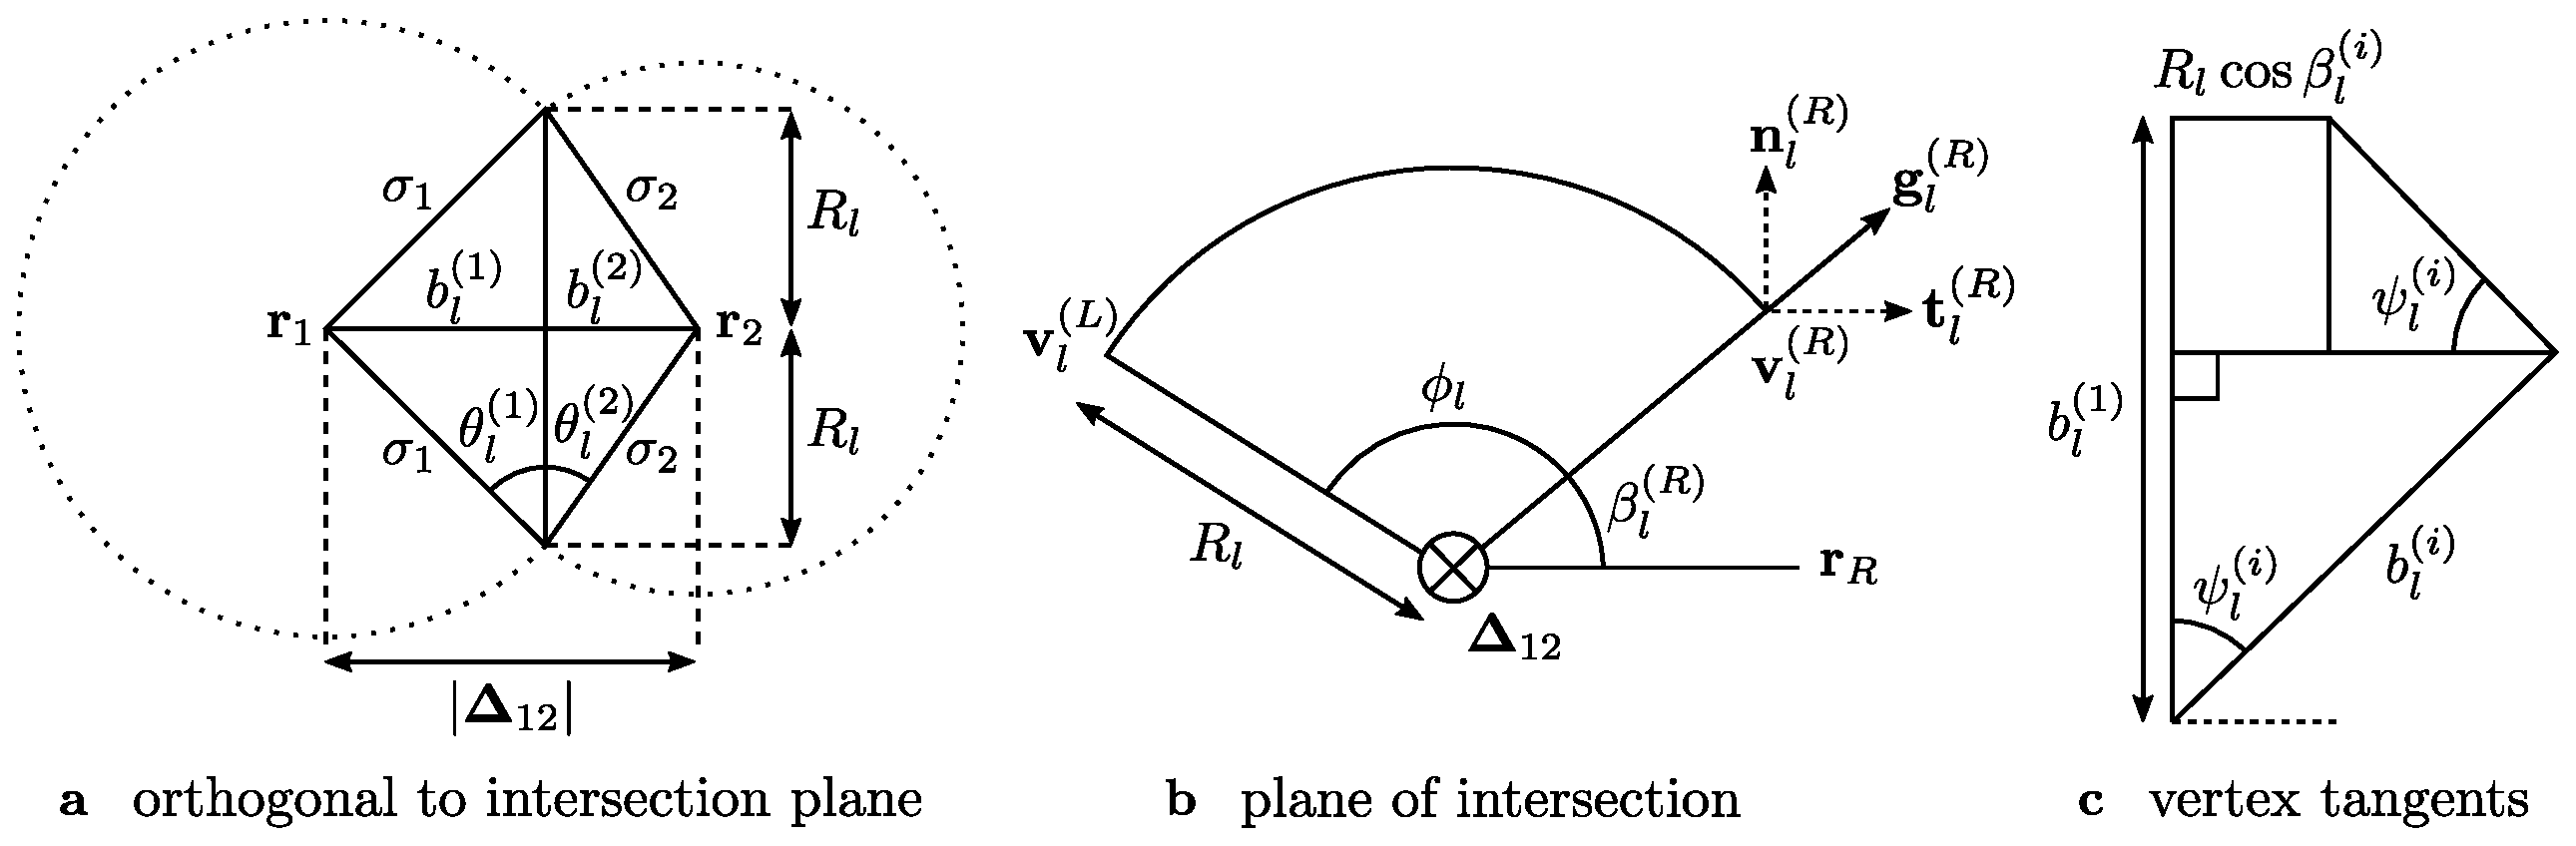
\includegraphics[width=\linewidth,outer]{curvature-geometry}
  \caption{Geometrical quantities involved in the calculation of line curvatures.}
  \label{fig:curvature-geometry}
\end{SCfigure}

\subsection{Particle separations}

The separation between two particle centers is
\begin{equation}
  \vec{\Delta}_{ij} = \vec{r}_i - \vec{r}_j
\end{equation}
which differentiates to
\begin{equation}
  \frac{\partial |\vec{\Delta}_{ij}|}{\partial r_k^\alpha} =
  \frac{r_i^\alpha - r_j^\alpha}{|\vec{\Delta}_{ij}|} (\delta_{ki} - \delta_{kj})
\end{equation}
where $\delta_{ij}$ is the Kronecker delta.

The basis vector for separations differentiates as
\begin{equation}
  \frac{\partial}{\partial r_k^\alpha}
  \left( \frac{\vec{\Delta}_{ij}}{|\vec{\Delta}_{ij}|} \right) =
  \frac{(\delta_{ki} - \delta_{kj}) \vec{e}_k^\alpha}{|\vec{\Delta}_{ij}|}
  - \frac{\vec{\Delta}_{ij}}{|\vec{\Delta}_{ij}|^2}
  \frac{\partial |\vec{\Delta}_{ij}|}{\partial r_k^\alpha}.
\end{equation}

\subsection{Quantities in the plane orthogonal to intersection}

We will label the particles whose intersection creates the circle of arc as 1 and 2 for convenience.
We consider the distances from these particles to the center of the circle as $b_l^{(1)}$ and $b_l^{(2)}$, see Fig.\ \ref{fig:curvature-geometry}(a).
Clearly $|\vec{\Delta}_{12}| = b_l^{(1)} + b_l^{(2)}$.
These distances form equilateral triangles with circle radius $R_l$ of hypotenuse $\sigma_i$ for $i \in \{1,2\}$.
This geometry is sketched in Fig.\ \ref{fig:curvature-geometry}a.
By Pythagoras' theorem we find the unknown distances as
\begin{align}
  R_l
  = \sigma_1 \, \cos{\theta_l^{(1)}}
  = \sigma_2 \, \cos{\theta_l^{(2)}}
  &= \frac{1}{2} \sqrt{
      2(\sigma_1^2 + \sigma_2^2) - |\vec{\Delta}_{12}|^2 -
      \left( \frac{\sigma_1^2 - \sigma_2^2}{|\vec{\Delta}_{12}|} \right)^2
    }, \\
  b_l^{(1)} = \sigma_1 \sin{\theta_l^{(1)}} &=
  \frac{ |\vec{\Delta}_{12}| + \frac{\sigma_1^2 - \sigma_2^2}{|\vec{\Delta}_{12}|} }{2}, \\
  b_l^{(2)} = \sigma_2 \sin{\theta_l^{(2)}} &=
  \frac{ |\vec{\Delta}_{12}| - \frac{\sigma_1^2 - \sigma_2^2}{|\vec{\Delta}_{12}|} }{2}.
\end{align}
The gradients of the angles between the planes are
\begin{subequations}
\begin{align}
  \frac{\partial \theta_l^{(1)}}{\partial r_i^\alpha} &=
  \frac{ 1 - \frac{\sigma_1^2 - \sigma_2^2}{|\vec{\Delta}_{12}|^2} }{2R_l}
  \frac{\partial |\vec{\Delta}_{12}|}{\partial r_i^\alpha}, \\
  \frac{\partial \theta_l^{(2)}}{\partial r_i^\alpha} &=
  \frac{ 1 + \frac{\sigma_1^2 - \sigma_2^2}{|\vec{\Delta}_{12}|^2} }{2R_l}
  \frac{\partial |\vec{\Delta}_{12}|}{\partial r_i^\alpha},
\end{align}
\end{subequations}
and the gradients of the distances are
\begin{subequations}
\begin{align}
  \frac{\partial R_l}{\partial r_i^\alpha} &=
  \frac{|\vec{\Delta}_{12}|}{4R_l}
  \left(
  \left( \frac{\sigma_1^2 - \sigma_2^2}{|\vec{\Delta}_{12}|} \right)^2 - 1 \right)
  \frac{\partial |\vec{\Delta}_{12}|}{\partial r_i^\alpha}, \\
  \frac{\partial b_l^{(1)}}{\partial r_i^\alpha} &=
  \frac{ 1 - \frac{\sigma_1^2 - \sigma_2^2}{|\vec{\Delta}_{12}|^2} }{2}
  \frac{\partial |\vec{\Delta}_{12}|}{\partial r_i^\alpha}, \\
  \frac{\partial b_l^{(2)}}{\partial r_i^\alpha} &=
  \frac{ 1 + \frac{\sigma_1^2 - \sigma_2^2}{|\vec{\Delta}_{12}|^2} }{2}
  \frac{\partial |\vec{\Delta}_{12}|}{\partial r_i^\alpha}.
\end{align}
\end{subequations}
As we must calculate the angles $\theta_l^{(1)}$ and $\theta_l^{(2)}$ and their derivatives for the curvature calculation, i.e.\ Eqs.\ \eqref{eq:integrated-curvature} and \eqref{eq:line-curvature-differential}, a convenient form for these latter derivatives is
\begin{subequations}
\begin{align}
  \frac{\partial R_l}{\partial r_i^\alpha} &
  = - b_l^{(1)} \frac{\partial\theta_l^{(1)}}{\partial r_i^\alpha}
  = - b_l^{(2)} \frac{\partial\theta_l^{(2)}}{\partial r_i^\alpha}, \\
  \frac{\partial b_l^{(1)}}{\partial r_i^\alpha} &=
  R_l \frac{\partial\theta_l^{(1)}}{\partial r_i^\alpha}, \\
  \frac{\partial b_l^{(2)}}{\partial r_i^\alpha} &=
  R_l \frac{\partial\theta_l^{(2)}}{\partial r_i^\alpha}.
\end{align}
\end{subequations}

The expressions in this section are the only quantities which explicitly depend on the sizes of the spheres $\sigma_i$, so we see how it is straightforward to consider the more general surface composed of arbitrarily sized spheres.
The above formulas are simplified if spheres are of equal sizes i.e.\ $\sigma_i = \sigma$ (as in the main text) leading to vanishing of $\sigma_1^2 - \sigma_2^2$ terms.

\subsection{Angular length}

To complete the derivatives in \eqref{eq:line-curvature-differential} we need an explicit expression for the gradient of the angular separation $\phi_l$.
In general, the line consists of an arc along a circle of radius $R_l$, which terminates at the vertices.
%It is possible for lines to not terminate at vertices, however we do not need to consider this special case as it occurs where $\phi_l = 2\pi$ is a constant so the gradient is zero and can be ignored.

We consider the 2d plane containing the intersection $S_1 \cap S_2$.
The center of the intersection circle is
\begin{equation}
  \vec{c}_l
  = \vec{r}_1 + b_l^{(1)} \frac{\vec{\Delta}_{12}}{|\vec{\Delta}_{12}|}
  = \vec{r}_2 - b_l^{(2)} \frac{\vec{\Delta}_{12}}{|\vec{\Delta}_{12}|}.
\end{equation}
The plane of intersection is seen by looking along $\vec{\Delta}_{12}$, making the arc $\phi_l R_l$ perfectly circular, shown in Fig.\ \ref{fig:curvature-geometry}b.
By convention we choose the arc to be a clockwise migration from a `left' vertex to a `right' vertex, which we label $v_l^{(L)}$ and $v_l^{(R)}$ accordingly.
These vertices form at 3-particle intersections, so we will use the suffixes $L$ and $R$ to indicate the 3rd particle index (distinct from 1 and 2) where appropriate.
We write the vertex coordinates as
\begin{equation}
  \vec{v}_l^{(i)} = \vec{c}_l + R_l \, \vec{g}_l^{(i)} \qquad i \in \{L,R\},
\end{equation}
where the unit vectors are
\begin{equation}
  \vec{g}_l^{(i)} =
  \frac
  {\vec{v}_l^{(i)} - \vec{c}_l}
  {|\vec{v}_l^{(i)} - \vec{c}_l|}
  \qquad i \in \{L,R\}.
\end{equation}
The unit vectors for the `right' component are sketched in Fig.\ \ref{fig:curvature-geometry}b.
The central angle is thus defined as the angle (going clockwise) between these unit vectors, i.e.
\begin{equation}
  \cos{\phi_l} = \vec{g}_l^{(L)} \cdot \vec{g}_l^{(R)},
\end{equation}
which after differentiation gives
\begin{equation}
  \frac{\partial \phi_l}{\partial r_i^\alpha} =
  - \frac
  {\frac{\partial \vec{g}_l^{(L)}}{\partial r_i^\alpha} \cdot \vec{g}_l^{(R)} +
   \vec{g}_l^{(L)} \cdot \frac{\partial \vec{g}_l^{(R)}}{\partial r_i^\alpha}}
  {\sin{\phi_l}}.
\end{equation}
So we need explicit expressions for vectors $\vec{g}_l^{(L)}$ and $\vec{g}_l^{(R)}$ and their derivatives to proceed.

We decompose the vertex unit vectors into the following Cartesian basis:
\begin{equation}\label{eq:vertex-unit-vector}
  \vec{g}_l^{(i)} =
  \cos{\beta_l^{(i)}} \, \vec{t}_l^{(i)} + \sin{\beta_l^{(i)}} \, \vec{n}_l^{(i)}
  \qquad i \in \{L,R\},
\end{equation}
where $\vec{t}_l^{(i)}$ is the vector tangent to the plane spanned by particles $\{1,2,i\}$ and $\vec{n}_l^{(i)}$ is normal to this plane.
If $\psi_l^{(i)}$ is the angle $\angle 1i2$, that is
\begin{equation}\label{eq:cos-psi}
  \cos{\psi_l^{(i)}} =
  \frac{\vec{\Delta}_{12} \cdot \vec{\Delta}_{1i}}
  {|\vec{\Delta}_{12}||\vec{\Delta}_{1i}|}
  \qquad i \in \{L,R\}
\end{equation}
then these basis vectors take the form
\begin{subequations}\label{eq:vertex-unit-vector-basis}
\begin{align}
  \vec{n}_l^{(L)} &=
  %\frac{\vec{e}_c \times \vec{e}_l}{|\vec{e}_c \times \vec{e}_l|} =
  \frac{1}{\sin{\psi_l^{(L)}}}
  \frac{\vec{\Delta}_{12} \times \vec{\Delta}_{1L}}
  {|\vec{\Delta}_{12}||\vec{\Delta}_{1L}|}, \\
  \vec{n}_l^{(R)} &=
  %\frac{\vec{e}_r \times \vec{e}_c}{|\vec{e}_r \times \vec{e}_c|} =
  \frac{1}{\sin{\psi_l^{(R)}}}
  \frac{\vec{\Delta}_{1R} \times \vec{\Delta}_{12}}
  {|\vec{\Delta}_{1R}||\vec{\Delta}_{12}|}, \\
  \vec{t}_l^{(L)} &=
  \frac{\vec{n}_l^{(L)} \times \vec{\Delta}_{12}}{|\vec{\Delta}_{12}|}, \\
  \vec{t}_l^{(R)} &=
  \frac{\vec{\Delta}_{12} \times \vec{n}_l^{(R)}}{|\vec{\Delta}_{12}|}.
\end{align}
\end{subequations}
Finally, from Fig.\ \ref{fig:curvature-geometry}c we have
\begin{equation}
  b_l^{(i)} \sin{\beta_l^{(i)}} - R_l \cos{\beta_l^{(i)}}
  = \frac{b_l^{(1)} - b_l^{(i)} \cos{\psi_l^{(i)}}}{\tan{\psi_l^{(i)}}}
  \qquad i \in \{L,R\},
\end{equation}
giving
\begin{equation}\label{eq:cos-beta}
  \vec{g}_l^{(i)} \cdot \vec{t}_l^{(i)} = \cos{\beta_l^{(i)}} =
  \frac{1}{R_l} \left(
    b_l^{(i)} \sin{\psi_l^{(i)}}
    + \frac{b_l^{(i)} \cos{\psi_l^{(i)}} - b_l^{(1)}}{\tan{\psi_l^{(i)}}}
  \right)
  \qquad i \in \{L,R\}.
\end{equation}

With explicit expressions for all of the vectors involved in the arc, the only remaining step is to differentiate.
First, we differentiate the vertex unit vectors Eq.\ \eqref{eq:vertex-unit-vector} in the basis defined by Eq.\ \eqref{eq:vertex-unit-vector-basis} to obtain
\begin{equation}
  \frac{\partial \vec{g}_l^{(j)}}{\partial r_i^\alpha} =
  \frac{\vec{g}_l^{(j)} \times \vec{\Delta}_{12}}{|\vec{\Delta}_{12}|} \,
  \frac{\partial \beta_l^{(j)}}{\partial r_i^\alpha} +
  \cos{\beta_l^{(j)}} \,
  \frac{\partial \vec{t}_l^{(j)}}{\partial r_i^\alpha} +
  \sin{\beta_l^{(j)}} \,
  \frac{\partial \vec{n}_l^{(j)}}{\partial r_i^\alpha}
  \qquad j \in \{L,R\}.
\end{equation}
Second, we take the derivatives of the basis vectors themselves Eq.\ \eqref{eq:vertex-unit-vector-basis} giving
\begin{subequations}
\begin{align}
  \frac{\partial \vec{n}_l^{(L)}}{\partial r_i^\alpha} &=
  \frac{\vec{e}_{c,j} \times \vec{e}_l + \vec{e}_c \times \vec{e}_{l,j}}{\sin{\psi_l}}
  - \frac{\cos{\psi_l}}{\sin{\psi_l}} \psi_{l,j} \, \vec{n}_l, \\
  \frac{\partial \vec{n}_l^{(R)}}{\partial r_i^\alpha} &=
  \frac{\vec{e}_{r,j} \times \vec{e}_c + \vec{e}_r \times \vec{e}_{c,j}}{\sin{\psi_r}}
  - \frac{\cos{\psi_r}}{\sin{\psi_r}} \psi_{r,j} \, \vec{n}_r,
\end{align}
\end{subequations}
Finally, we differentiate the angles from Eqs. \eqref{eq:cos-psi} and \eqref{eq:cos-beta} to get
\begin{subequations}
\begin{align}
 \frac{\partial \beta_l^{(j)}}{\partial r_i^\alpha} &=
  \frac{
  \frac{\partial R_l}{\partial r_i^\alpha}
  \cos{\beta_l^{(j)}} -
  \frac{\partial}{\partial r_i^\alpha}
  \left( R_l \cos{\beta_l^{(j)}} \right)}
  {R_l \sin{\beta_l^{(j)}}}, \\
 \frac{\partial}{\partial r_i^\alpha}
  \left( R_l \cos{\beta_l^{(j)}} \right) &=
  \frac{1}{\sin{\psi_l^{(j)}}}
  \frac{\partial b_l^{(j)}}{\partial r_i^\alpha}
  - \frac{1}{\tan{\psi_l^{(j)}}}
  \frac{\partial b_l^{(1)}}{\partial r_i^\alpha}
  - \frac{b_l^{(j)} \cos{\psi_l^{(j)}} - b_l^{(1)}}
  {\sin^2{\psi_l^{(j)}}}
  \frac{\partial \psi_l^{(j)}}{\partial r_i^\alpha}, \\
  \frac{\partial \psi_l^{(j)}}{\partial r_i^\alpha} =
  -\frac{1}{\sin\psi_l^{(j)}} \frac{\partial(\cos{\psi_l^{(j)}})}{\partial r_i^\alpha} &=
  -\frac{1}{\sin\psi_l^{(j)}}
  \left(
  \frac{\partial}{\partial r_i^\alpha}
  \left( \frac{\vec{\Delta}_{12}}{|\vec{\Delta}_{12}|} \right) \cdot
  \frac{\vec{\Delta}_{1j}}{|\vec{\Delta}_{1j}|}
  +
  \frac{\vec{\Delta}_{12}}{|\vec{\Delta}_{12}|} \cdot
  \frac{\partial}{\partial r_i^\alpha}
  \left( \frac{\vec{\Delta}_{1j}}{|\vec{\Delta}_{1j}|} \right)
  \right),
\end{align}
\end{subequations}
for $j \in \{L,R\}$ in each expression.

\section{Integrated Gaussian curvature}

$\partial\mathcal{L}$ forms a closed two-dimensional surface, so by the Gauss-Bonnet theorem \footnote{\url{https://www.encyclopediaofmath.org/index.php/Gauss-Bonnet_theorem}} the integrated Gaussian curvature must be
\begin{equation}\label{eq:gauss-bonnet}
  X_{\partial\mathcal{L}} = 2\pi \chi
\end{equation}
where $\chi$ is the Euler characteristic of $\partial\mathcal{L}$, a topological constant of the surface.
Thus, the derivative of $X$ is zero everywhere except at pathological points where a topological change in the surface occurs.
In practice this happens when a cavity larger than a particle size forms inside the structure, or when a particle dissociates; being interested in \emph{compact} local structures, we can exclude both of these scenarios from consideration.
Thus, for all local structures $\chi=2$, and the gradient of $X$ is zero everywhere.

Under the above assumptions we do not need to compute $X_{\partial\mathcal{L}}$, but nevertheless it is convenient to do so in order to check the correctness of the algorithm:
\begin{equation}
  X_{\partial\mathcal{L}} =
  -\sum_{l \in L} \phi_l (\sin{\theta_l^{(1)}} + \sin{\theta_l^{(2)}}) +
  \sum_{(i,j,k) \in V} \Omega_{ijk}
\end{equation}
where $\Omega_{ijk}$ is the solid angle spanned by the 3-vectors at vertex $S_i \cap S_j \cap S_k$ \cite{MeckeAA1994}.
The condition that this sum must produce the same result as \eqref{eq:gauss-bonnet} provides a useful check of the numerics.

\section{Intersections of more bodies: possible caveats with quenched geometries}
\label{sec:higher-order-intersections}

A common task with computer simulations is to quench a geometry to find the minimal (or \emph{inherent}) energy structure.
Quenched geometries are inherently athermal so the argument above that intersections of $n>d$ spheres should occur with vanishing probability does not apply; it is common to find intersections of 4 or more particles at the surface in $d=3$ \emph{after a quench}.
To investigate quenched geometries one must properly treat such intersections, as we will demonstrate below with an illustrative example.

An example of these intersections in $d=3$ occurs where 4 particles are arranged in a perfect square (as in e.g.\ any outer face of the body-centered cubic unit cell).
This special geometry corresponds to a bifurcation point in configuration space, where two pairs of surface vertices are simultaneously created and annihilated.
The gradient is not continuous at these points \emph{with respect to the atomic coordinates}, as the continuity of the morphological free energy is only guaranteed with respect to the set $\mathcal{L}$ according to the Hausdorff metric.
In atomic coordinates derivatives can contain poles and step discontinuities.

As the example above illustrates, the gradient is not well defined at pathological points where many spheres intersect.
It is thus impossible to quench these geometries using standard algorithms (which assume smooth functions) and perturbation theories (e.g.\ the harmonic approximation for the free energy) will fail.
A proper treatment of these cases would be required for an investigation of quenched geometries.
In this work we have avoided these considerations primarily by restricting ourselves to geometries thermalised using a Monte-Carlo algorithm (Figures \ref{fig:structure-populations} and \ref{fig:reaction} in the main text).
Construction of the reaction path of $n=6$ particles necessitates an analytic method which uses a quenched geometry, however the geometries for $n=6$ are not pathological so no special consideration is needed.

\ifdefined\includebibliography
  \printbibliography
\fi

\end{document}

\end{appendices}

\printbibliography[heading=bibintoc]

\end{document}
}
\definecolor{bristolred}{RGB}{191,47,56}

\begin{document}

\newgeometry{margin=1in}

%\maketitle
\thispagestyle{empty}
\begin{center}
  \begin{minipage}{0.8\linewidth}
    \centering
    %
\includegraphics[width=0.6\linewidth]{bristol-logo}\par
    %\rule{0.4\linewidth}{0.15\linewidth}\par
    \vspace{3cm}
    %\hline
    {\Large \sc University of Bristol \par}
    \vspace{2cm}
    {\Large \sc Doctoral Thesis \par}
    \vspace{1cm}
    \rule{\textwidth}{0.4pt} \par
    {\LARGE \sc \color{bristolred} Some equilibrium approaches to the high-density liquid (working title) \par}
    \rule{\textwidth}{0.4pt} \par
    %\hline
    \vspace{2cm}
    {\large \it Author:}
    \hfill
    {\large \it Supervisor:} \\
    {\sc \large \href{mailto:joshua.robinson@bristol.ac.uk}{Joshua F.\ Robinson}}
    \hfill
    {\sc \large Prof.\ C.\ P.\ Royall \par}
    \vspace{3.5cm}
   {\large \it A dissertation submitted to the University of Bristol in accordance with the requirements for award of the degree of Doctor of Philosophy in the Faculty of Science, H.\ H.\ Wills Physics Laboratory. \par}
    \vspace{1em}
    {\large August 2019 \par}
  \end{minipage}
  \mbox{}
  \vfill
  \begin{minipage}{0.8\linewidth}
    \raggedleft
    {\large \wordcount words}
  \end{minipage}
\end{center}

\pagenumbering{roman}
\cleardoublepage\chapter*{Abstract}
\addcontentsline{toc}{chapter}{Abstract}

This dissertation describes an investigation into methods for advancing understanding of liquids at high densities, where dynamical processes become highly non-trivial.
Specifically, we address structure in supercooled liquids approaching their glass transition, and the kinetics of nucleating the stable cystal phase.
In both cases we describe the liquid using equilibrium physics, even though the system is metastable and not strictly in equilibrium.
The first three results chapters focus on the supercooled liquid, while the final results chapter addresses nucleation.

In the first part comprising three chapters, we combine geometric techniques with liquid state theory to develop an approach for treating complex many-particle local structures inside the bulk hard sphere liquid.
We introduce the \emph{morphometric approach}, a liquid state theory based on integral geometry, as a means of calculating many-body correlation functions.
We argue for the morphometric approach from several routes, and derive multiple specific theories for hard spheres including one suitable for producing accurate correlation functions.
We later derive the morphometric approach for hard spheres from first-principles using the virial series.
This places the approach on more rigorous ground, and suggests routes to extending the theory as part of a controlled expansion.

With the resulting many-body correlation functions, we are able to predict the concentrations of complex many-particle structures in the bulk liquid; these results are of particular relevance to theories of supercooled liquids and glasses.
We find a bimodality in the energy landscape for hard sphere local structures, where fivefold symmetric structures appear lower in free energy than fourfold symmetric structures.
In addition, we develop similar techniques for predicting the thermodynamic barriers to dynamical processes inside the bulk system.
The solution to the overarching problem of predicting structure formation inside a bulk system has potential to advance study of self-assembly, nucleation and protein folding in aqueous environments.

In a final part we address nucleation of salt crystals in drying aerosol droplets, of particular relevance to climate models and industrial spray drying applications.
Treating the droplet in the continuum limit, we solve the diffusion equation with moving boundary conditions.
By comparison with experimental data we are able to assess the accuracy of classical nucleation theory, with mixed success depending on the system.
%% We find it successfully predicts the nucleation kinetics of \ce{NaCl} aerosol droplets but fails for \ce{NaNO3}.
%% We find a complex interplay between inhomogeneity of the droplet concentration profile and droplet temperature affects the nucleation kinetics.

\cleardoublepage\chapter*{}
\vspace*{0.2\textheight}
\begin{center}
\noindent\emph{Dedicated to all of the cats of the internet, whose rheological properties inspired this delve into liquids.}
\end{center}

\cleardoublepage%\restoregeometry

\chapter*{\vspace{-1em} Acknowledgements}
\addcontentsline{toc}{chapter}{Acknowledgements}

First and foremost, I want to thank my supervisor, Paddy, for being the reason that any of this happened at all, for being a crucial check on my natural impulse to be \emph{too} focused on details and for the fact that I now see beautiful (pink) icosahedra everytime I close my eyes.
I thank him for giving me the freedom to develop my ideas, and for his remarkable degree of patience when that led to me studying six particles for four years.

It has now been several years since Paddy gave me the `humble' task of solving the glass transition once and for all.
Having failed spectacularly at this, I hope we can collectively agree that the real glass transition was the friends we made along the way.
In particular, all of the cave-dwellers (and countless mice) of G.39 who survived the water features, two fumigations and Paddy.
The forces of darkness may have stolen our toaster, but they never broke our spirit%
\footnote{After all, we had the science to do that.}.
I will treasure these memories, and your friendship, until the end of my days.
%Honorable mentions to the contriband toaster and the electric fence of Fowey.
%Together we braved the near-total sunlight deprivation, more mice than I care to remember and an incident with an electric fence.
%Special thanks go out to the electic fence which our trip to cornwall.

I owe a great debt to Francesco Turci for dedicating far more time than I deserve to discuss my work.
I honestly don't think I could have done this without his consistent, valuable input throughout.

I would like to express my gratitude to our collaborator Roland Roth, for founding the Bristol's White Bear institute, conjuring up the initial idea for my project with Paddy and providing guidance along the way.
Additionally, I am deeply grateful to our collaborators in chemistry for what turned out to be a fun and fruitful project: Flo Gregson, Rachel Miles and Jonathan Reid.
I especially thank Flo for doing the experiments which made this collaboration possible, and for providing valuable feedback on my initial attempts at describing them in chapter \ref{chapter:aerosols}.

Special thanks go out to Bob Evans, who showed interest in my work from the very beginning, for the many stimulating discussions about liquid state theory over the years.
I must also thank him for the constructive feedback he gave on an early draft of the paper underlying parts of chapters \ref{chapter:morphometric-framework} and \ref{chapter:morphometric-applications}.
I recall he described me as ``completely mad'' afterwards, which I \emph{think} was a compliment, so I must additionally thank him for inadverently suggesting an `insanity defence' to rely upon in my viva.

I am very grateful to the organisers and lecturers at the Boulder School in Condensed Matter and Materials Physics 2017.
This school influenced my development as a statisical physicist in a myriad of ways.
Notably, I found myself referring back to the phenomenological lectures by Gilles Tarjus while writing chapter \ref{chapter:glass}.

Financially, I acknowledge the European Research Council under the FP7 / ERC Grant Agreement No.\ 617266 ``NANOPRS'' and Paddy for finding ways to support me after this ran out.

I have learned that research is an almost constant uphill struggle, with the occasional false summit.
My most heartfelt appreciation goes out to all my friends and colleagues who made the struggle worthwhile.
I would particularly like to thank Kate Oliver, Nick Wood and Max Meissner for keeping me sane in difficult times, and Kirsty Wynne for teaching me perspective and the meaning of a `false summit'.
Last, and certainly not least, I owe my deepest gratitude to all the close friends and family members who were there for me every step along the way.

%\newgeometry{margin=1in}

\cleardoublepage\chapter*{Declaration}
I declare that..

\cleardoublepage\chapter*{}
\vspace*{0.2\textheight}
\begin{center}
\noindent\enquote{\itshape Keep cool, never freeze.}\hspace{1.5cm} \bigbreak

\hspace{1.5cm} -- Hellmann's\textsuperscript{\textregistered} mayonnaise bottle.
\end{center}


\cleardoublepage\tableofcontents
\cleardoublepage\listoffigures
\cleardoublepage\listoftodos

\restoregeometry

\pagenumbering{arabic}
\setcounter{page}{1}
%TC: macro \marginfootnote [other]
%TC: envir SCfigure [] other
%TC: macrocount beginSCfigure [figure]
\documentclass[11pt,twoside]{report}
\usepackage{preamble}
\setcounter{chapter}{0}
\graphicspath{{../img/}}
\def\includebibliography{}

\begin{document}
\chapter{Introduction}
\epigraph{Everything starts somewhere, though many physicists disagree.}{Terry Pratchett, \emph{Hogfather}, (1996).}

\section{Overview}

%Begin with a short (1–2 pages) broader introduction for a general audience: one that my mother could understand so she knows what I’ve been working on all these years.

What precisely is covered by soft matter, and how to properly demarcate, is a matter of some academic debate.
In some sense soft matter can be most easily understood by : it is the science of ``squishy'' things.
The eminent soft matter physicist Wilson Poon describes soft matter as ``liquids with bits'' in them.
A more precise and scientific definition posits that the energy scale is subject to thermal fluctuations.
So e.g.\ chemical bonds break and reform allowing flow, but the physical processes may be arbitrarily more complex than simple liquids.

Soft matter was clearly preceded by liquids, and it is up to the individual whether liquids should be considered as the antecedent to or subsumed by soft matter.
My personal bias is that liquids represent a subset of soft matter, the zeroth order approximation to real systems.

\section{Simple liquids}

Physics is filled with toy models.
The Ising model is the most widely studied magnetic model, and the usual starting point for students learning statistical mechanics/phase transitions particular the critical point where this is \emph{the} model system.

What are simple liquids, with hard spheres at the forefront.
\hl{Hard spheres serve as a good touchstone for some of the fundamental knowns and controversies in liquid state theory and, by extension, soft matter.}
The physicists favourite toy model is the hard sphere liquid.
Interaction potential is the no-overlap condition%
\marginfootnote{I like to imagine them as ideal billiard balls, i.e.\ without any dissipative forces like friction so they continue to bounce off one another forever.}:
\begin{equation}
  U =
  \begin{cases}
    \infty & \; r < \sigma \\
    0 & \; \textrm{otherwise}.
  \end{cases}
\end{equation}
As the potential is everywhere zero or divergent, temperature has no effect on the interactions making this system athermal.
Instead, the natural control parameter is (number) density $\rho = N/V$, or as it is normally rescaled into volume fraction: the volume of space occupied by the spheres i.e.\
\begin{equation}
  \eta = \frac{N v}{V} = \rho v
\end{equation}
where $v$ is the volume of a single hard sphere.

When van der Waals wrote down their famous equation of state for real gases, i.e.\
\begin{equation}
  (p - a N)(V - Nv) = N k_B T
\end{equation}
where $V - Nv$ corrects for the volume occupied by finite-sized particles and $p - aN$ for the interactions,
it was widely believed that to go beyond this to understand liquids more sophisticated treatments of the \emph{attractions} would be required.
History shows that in actual fact the treatment of \emph{repulsions} were lacking.
It turns out that to a large degree simple liquids can be considered as hard spheres plus an attractive perturbation: an accurate treatment of the repulsion is needed, attractions can be less accurate.

\begin{SCfigure}
  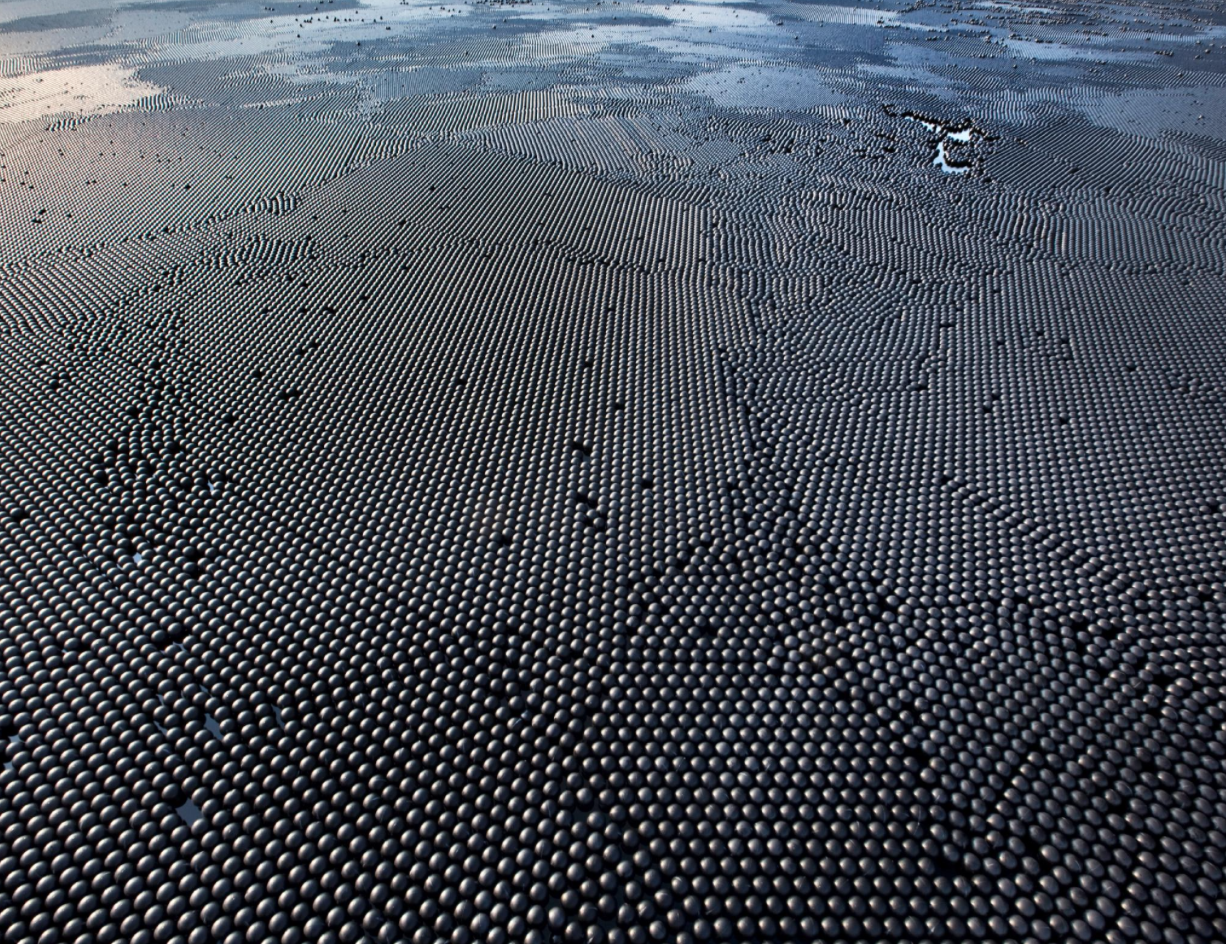
\includegraphics[width=0.75\linewidth,outer]{shade-balls}
  \caption[Shade balls floating on water: a 2d `crystal']{
    Shade balls covering the Los Angeles reservoir to cool water preventing evaporation and certain light-activated chemical reactions at the water surface.
    As macroscopic objects these balls interact as hard spheres, and they spontaneously form long-ranged orientational order seen as hexagonal domains.
    This is reminiscent of crystallisation in atomic systems.
    Image by Gerd Ludwig, \emph{National Geographic} (2007).}
  \label{fig:shade-balls}
\end{SCfigure}

Despite their coarse simplification of real atomic interactions, we see that hard spheres actually capture a lot of the essential physics.
To illustrate this consider the phase diagram of hard spheres Fig.\ \ref{fig:hs-phase-diagram}.
We see there is a freezing transition at $\eta = 0.494$, suggesting that the liquid will spontaneously order into a crystal at high densities.
This is surprising, in everyday scenarios (e.g.\ water) we are used to seeing crystallisation as one lowers temperature and the explanation normally given in classrooms is that the crystal is favoured due to attractions between molecules.
Now, in real systems crystallisation can also be triggered by changes to density also so density being a control parameter is not a problem, however the lack of attractions should, if this intuition were correct, prohibit crystallisation.

It turns out in the case of hard spheres that the crystal has a larger entropy above freezing, so entropy itself triggers crystallisation.
This was a hotly debated topic \cite{?,?,?} until is was solved by computer simulation in \cite{?,?,?} and experiment \cite{?,?,?}.
Part of the reason people could not believe that the crystal is entropically favoured, is because we often mistakenly take entropy to be a measure of disorder when it in fact more complicated.
The crystal might be more ordered than the liquid, with a lower \emph{configurational} entropy, however the entropy includes \emph{all} microstates not just averaged ones: the crystal is compensated by having a much larger \emph{vibrational} entropy than the liquid at high densities.
Including both these contributions leads to the phase diagram that we know today.

A similar effect is seen in balls floating on water as in e.g.\ peas in a saucepan or shade balls covering a reservoir.
The hard interactions between the balls causes%
\marginfootnote{In an attempt to find an everyday example, I have taken liberties with the interaction being purely hard; I suspect that floating balls feature effective attractions due to \emph{hydrodynamic} interactions at the water surface.}[-3cm]
them to `crystallise' at high densities as seen in Fig.\ \ref{fig:shade-balls}..
Strictly speaking these are not crystals in the sense of long-range \emph{translational} order, instead they are said to possess long-range \emph{orientational} order.
This subtlety emerges because the floating balls are confined to the water surface making them effectively two dimensional; fluctuations are strong enough in two dimensions to overcome truly long-ranged positional ordering \cite{MerminPRL1966,MerminPR1968}.

We have extolled the virtues of hard spheres, however this should not be interpretted as saying that this model system capture \emph{all} of the physics of real systems: it is a toy system after all.
They are merely a very good starting point for more complex systems.
As an example of physics they do \emph{not} capture, consider the critical point of real liquids.
Liquid-gas critical phenomena emerges from a competition between attractive and repulsive forces, with divergent fluctuations at the critical point.
It is thus impossible for a system with purely repulsive interactions, like hard spheres, to feature a critical point.
That being said, many theories predict critical phenomena quite well by taking a hard sphere potential and incorporating a mean-field like attractive perturbation \cite{?} so a hard sphere system provides a good reference point.

Hard spheres exist in more than just a theorist's imagination: they can be experimentally realised in colloidal experiments.
Colloidal suspensions are mixtures of solute immersed in a solvent composed of much smaller particles.
Colloidal particles are typically at the micron-scale.
These typically feature complex interactions \cite{Royall?,?,?} however these can be tailored to closely approximate hard sphere like interactions through steric stabilisation.
\todo{What is an aerosol? What is a dispersion?}
Colloidal experiments closely match hard simulations and theoretical predicitons \cite{?}.
Notably one can determine the phase diagram see Fig.\ \ref{fig:hs-phase-diagram}.
Note the glass at very high densities.

\begin{SCfigure}
  \missingfigure[figwidth=\linewidth]{}%
  \caption[The hard sphere phase diagram]{
    The hard sphere phase diagram, including the metastable branch.
    a: theoretical phase diagram.
    b: experiments, including the glass (image reproduced from \cite{?}).
    This is one of the most iconic images in the field, and no discussion of colloidal hard spheres would be complete without it.}
  \label{fig:hs-phase-diagram}
\end{SCfigure}

\begin{SCfigure}
  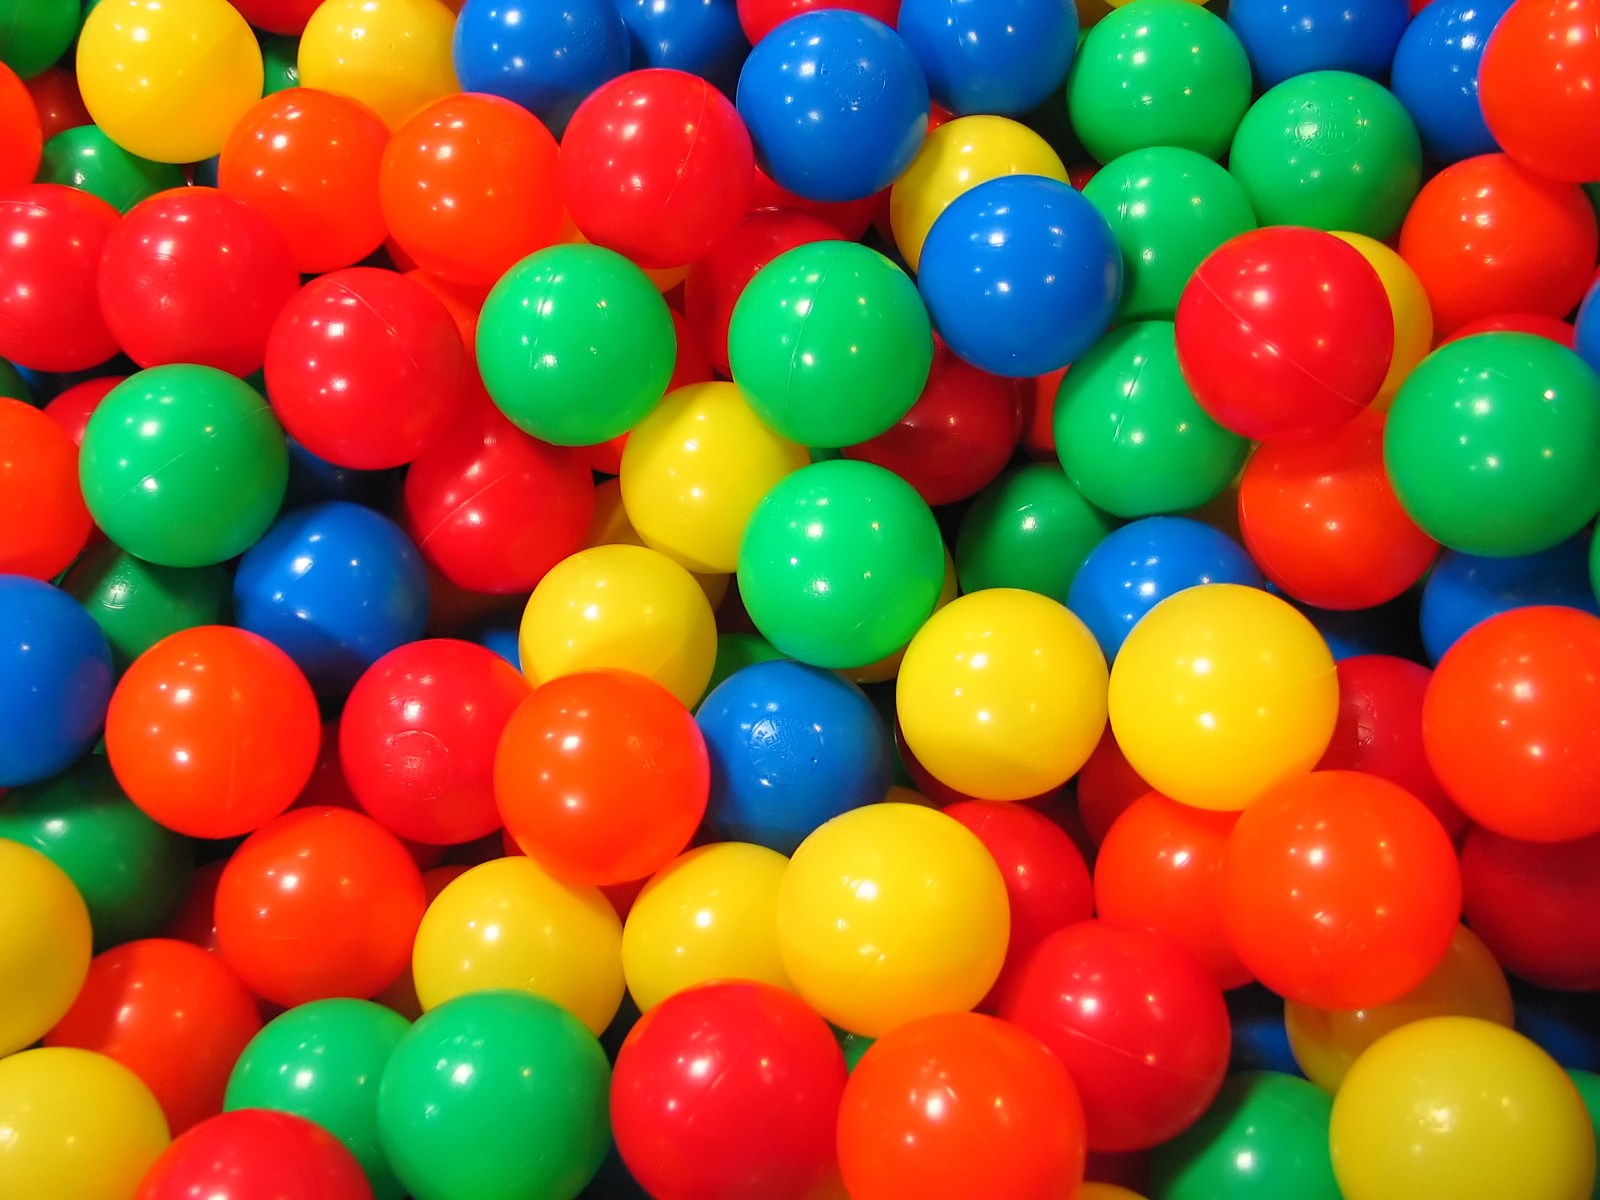
\includegraphics[width=0.75\linewidth,outer]{ball-pit-horizontal}
  \caption[Random close packing in a ball pit]{
    Random close packing of hard spheres in a ball bit.
    Image by Peter Ong.}
  \label{fig:rcp}
\end{SCfigure}

As the most widely studied model interaction potential we know a lot about its equilibrium structure (phase diagram) in bulk and even inhomogeneous thanks to density functional theory \cite{?,?,?}.
However, its behaviour off-equilibrium at high densities is hotly debated.
The two biggest unresolved research topics for this subject:
\begin{itemize}
\item \emph{Nucleation}: given that above freezing the crystal ? Theoretically predicted nucleation rates from simulation studies differ by 12 orders of magnitudes from experiments, purported to be the second biggest disagreement between theory and experiment in all of science \cite{?}.
\item \emph{Metastable liquid}: if one could avoid crystallisation and equilibrate only over the liquid microstates, what would be the ultimate fate of the liquid?
  We will talk more about this in \ref{?}.
\end{itemize}

There is a deep connection between hard spheres and computer science.
Packing problems have been studied \cite{Cohn,Conway,Sloane} and they are notoriously difficult; Kepler conjectured the optimal packing in 3d was the face-centred cubic/hexagonal close packing but it took 300(?check) years to solve this.
The final proof was computer aided, and not simple.
Packing problems are connected with encoding/encryption.
Transmitting a signal requires a way to encode a message across a band(?): if packed too tightly on the band(?) then noise will destroy the signal to it is desirable to optimise the sites for bits \cite{Cohn,?,?}.
Additionally, lattice based encryption techniques are one of the alternatives to prime factorisation: the coming development of quantum computers \cite{?,?} would render prime factorisation easy because of Shor's algorithm \cite{Shor?} rendering standard encryption techniques insecure.
The techniques developed for the mean field hard sphere problem have been applied to the perceptron model \cite{?}, and deep-learning neural networks which are naturally high dimensional problems lending themselves to a mean field treatment \cite{?}.

\begin{SCfigure}
  \includegraphics[width=0.75\linewidth,outer]{cannonballs}
  \caption[Close packed cannonballs]{
    Sketch of close-packed stacks of cannonballs in Fortress Monroe.
    Image by Stacy, \emph{Harper's weekly} (1861)}
  \label{fig:fcc}
\end{SCfigure}

Although hard spheres will be our focus, we will mention the importance of systems of hard particles of other shapes for self-assembly.
Self-assembly is an active area of soft matter: it is technologically desirable to tailor the final structure by controlling the building blocks.
Imagine assembling nanomachines or artificial cells by controlling the chemistry.
It is found that varying the size and shape of hard particles can reproduce all the complexity of the periodic table \cite{Glotzer?,Dijkstra?}.
Hard spheres are the simplest such system, so a theory which can treat other geometries is desirable.

The primary goal of this thesis is to advance the methods of treating liquids at high densities, particularly concerning the role of thermodynamics in dynamical arrest and nucleation.
These methods can be readily adapted to more complex systems, such as protein folding in aqueous solution or self-assembly of complex structures.

A secondary goal would be to advance the understanding of the fundamental theory of hard particles in some small way.
I have attempted to develop the geometrical theory behind the methods of Chapters \ref{?} and \ref{?} in a generally applicable way;
I have done this to the best of my ability, but my primary skills lie in numerical methods and I am a second-rate theoretician.

\section{Supercooled liquids and glasses}

It is widely reported that glass is actually liquid, and as evidence of this the thickness of old windows at the bottom is pointed to.
This is actually a matter of some dispute, but contains a grain of truth.
Pre-modern methods of creating window glass involved spinning molten glass on magma to flatten it out.
Centrifugal forces caused the glass to be thicker on the outer disk, so panes of glass would always be heavier in one direction%
\marginfootnote{And personally, if I were setting an uneven pane of glass I would place the heavy part at the bottom.}.

To a soft matter physicist glass is a broader term, referring to a wide class of materials while the window glass of common parlance is referred to by its chemical name \emph{silicate}.
This class of materials share many features of being disordered etc \cite{?} although in some sense they are connected by what they do \emph{not} do: which is flow on human timescales.
When I refer to `glass' I will be using it in this broad technical sense of a state of matter.
Some examples besides silicate:
\begin{itemize}
\item Most of the ice in the universe exists in an amorphous state in comets \cite{?}
\item Ceramics
\item Plastics: amorphous polymers
\end{itemize}
Of more abstract nature which could be called glassy though they are not materials
\begin{itemize}
\item Gels: super glasses, liquid like bit plus a network/backbone which has glassy dynamics
\item Neural networks
\item Non-deterministic polynomial time (NP) problems
\end{itemize}
We will not be directly addressing the latter type of more abstract problems which could be considered glasses, although they are arguably related due to a similar underlying disorder.
We will be focusing on only the most rudimentary of glassy phenomenology: the dynamical arrest of liquids at high densities/low temperatures when crystallisation is avoided.
Especially as it manifests in hard spheres, which as discussed is the reference system of choice for simple liquids.

So what do we mean by dynamical arrest.
Typically we can look at one of two (related) quantities: viscosity or relaxation time.
Viscosity measures how resistant the thing is to flow, while relaxation time measures the typical microscopic time for things to move around i.e.\ liquid like behaviour.
As a practical definition, a glass is defined in the lab as any material for which the relaxation time exceeds 100\ce{s}: this point is called the experimental glass transition.
This is somewhat arbitrary, although the location of the glass transition point is not particularly sensitive to where you set the threshold because of how rapidly the viscosity/times are increasing around there.
\todo{Need: Angell plot, fragile vs strong}

Personally, the observation that got me interested in the field is the entropy argument.
If one compares the difference between the entropy of the crystal and the glass, and extrapolates wildly one expects there to be a point where the glass has a lower entropy than the crystal.
This is not very meaningful by itself, as we have already established by discussing the crystal vibrational entropy can be quite subtle so it is possible for the liquid to have a lower vibrational entropy.
However, if one corrects this with more modern techniques to measure just the entropy corresponding to non-trivial motion we see that there is a point where the configurational (i.e.\ not purely vibrational) entropy vanishes: this would imply the system is frozen in a single configuration.
Such a point would define a transition to a genuine thermodynamic phase, an ideal glass.
\todo{Plots of configurational entropy}

A diverging timescale necessarily requires a diverging point-to-set length scale and a vanishing configurational entropy, a proof given in \cite{?}.
This must trivially occur at the very least $T=0\si{K}$ where relaxation timescales diverges, however much like the lack of a phase transition in the Ising model in $d=1$ this is not a true thermodynamic phase transition because it cannot be crossed.
Recent numerical evidence suggests that a model glassformer in $d=2$ does not show a transition, also vanishing at $T=0\si{K}$ \cite{Berthier?}.
So the central question of glass is what happens in $d=3$, is there a vanishing configurational entropy at a finite $T > 0$ with an accompanying thermodynamic glass transition?
In mean-field, formally in the limit of infinite spatial dimensions $d \to \infty$, the hard sphere system has been shown to have a true transition, however the critical dimensions are unknown so it is unclear what happens in $d=3$ \cite{Parisi,Zamboni,Charbonneau,Kurchan,?,?}.

\todo{Jamming: how does it relate to glass}

\section{Notes from Tarjus}

Overview of the glass transition.
Salient features: why hard, interesting, unique.

What is a glass?
Frozen in a (apparently) disordered state.
All sorts of glasses, structural, spin, orientational, electron, vortex.
Glasses formed by liquids, colloidal suspensions and polymers: traditional structural glasses.
Solid: doesn't flow on observational time, resists small/infinitesimal shear (acts like solid).
Amorphous, apparently amorphous: no periodic arrangement like in crystal.
Homogeneous makes useful for technology: useful for e.g.\ optical properties.

Hard glasses: high elastic constants.
Colloidal suspensions: soft matter version, small elastic constants.
Same phenomenology though.

Cooling a liquid.
Take thermodynamic quantity (e.g.\ volume, entropy, enthalpy): usually crystallise.
(Picture)
First-order transition bypassed by quick cooling.
Enter supercooled liquid phase.
No longer equilibrates/relax/flows, call it a glass: occurs at glass transition.
Glass is a solid for all practical purposes.

SC liquid: same characteristics as at equilibrium.
Independent of preparation: loses memory of initial preparation.
Measureable properties have time translational invariance/are stationary.
Time independence of all observables, i.e.\
\begin{equation}
  \langle A(t) \rangle = \langle A \rangle
\end{equation}
including correlation functions e.g.\
\begin{equation}
  \langle A(t) A(t') \rangle = \langle A(0) A(t - t') \rangle
\end{equation}
(equation for stationary)
Fluctuation-dissipation theorems.
Linear response regime: response to perturbation related to correlation function (spontaneous fluctuations).
\begin{equation}
  \chi_A (t, t')
  =
  - \beta \Theta(t - t')
  \frac{d}{dt}
  \left(
  \bigg\langle
  (A(t) - \langle A \rangle)
  (A(0) - \langle A \rangle)
  \bigg\rangle
  \right)
\end{equation}

\ifdefined\includebibliography
  \printbibliography
\fi
  
\end{document}

%TC: macro \marginfootnote [other]
%TC: envir SCfigure [] other
%TC: macrocount beginSCfigure [figure]
\documentclass[11pt,twoside]{report}
\usepackage{preamble}
\setcounter{chapter}{1}
\graphicspath{{../img/}}
\def\includebibliography{}

\externaldocument{morphometric-framework}

\begin{document}
\chapter{Background}
%\epigraph{It tells me that the Creator used the wrong kind of circles.}{Terry Pratchett, \emph{Pyramids} (1989).}
\epigraph{It was not certain what significance the ceremony held... but the formality was no less sacred for it being unintelligible}{Mervyn Peake, \emph{Titus Groan}, (1946).}

In this chapter we provide a \emph{concise} account of the foundational frameworks underlying the two themes of this thesis: \emph{integral geometry} and \emph{liquid state theory}.
I expect the reader to have a background in statistical physics, so my account of liquid state theory is not intended to be exhaustive; for more in-depth treatments see the references herein.
By contrast, I do \emph{not} expect much familiarity with integral geometry.
Understanding the underlying mathematical detail is not essential to follow the rest of the thesis, so I will focus more on the key concepts and notation than detailed derivation.
I anticipate the expert reader will skim over this chapter, so I have placed the important theorems in boxes as a guide to the most relevant parts.

As many-body correlation functions are a central theme of the results chapters, I have emphasised correlation functions in section \ref{sec:liquid-structure} on liquid structure to the point where I have somewhat belaboured giving the explicit forms and normalisations of the various correlation functions.
Even though we will only use one particular hierarchy of correlation functions in the results chapters, I personally found it helpful to have these formulas in one place.
I have found myself frequently revisiting the transformations between the various hierarchies of correlation functions, so I include them in anticipation that someone repeating or extending this work can profit from having a kind of ``cheat sheet''.

\section[Integral geometry. Or ``How long is a piece of string?'']{Integral geometry\\ {\large Or ``How long is a piece of string?''}}
\label{sec:integral-geometry}

\subsection{Towards a geometric interpretation of extensivity}

Geometry has been a recurring theme in physical theories, appealing because of its intuitive nature.
There are many ways that geometric ideas can be incorporated, but our focus will be on expansions of thermodynamic quantities in terms of \emph{sizes}.
The usefulness of this particular focus is directly connected to the familiar concept of \emph{extensivity} in statistical mechanics, which we will use to guide the following discussion.
Thermodynamic potentials must be extensive to remain well-defined in the thermodynamic limit,
%Defining an extensive quantity as one that scales proportionally to system size, the first meaning of size that comes to mind is probably the volume.
so by focusing on extensive quantities we ensure a thermodynamically consistent description in this limit.

%The first notion of size that likely comes to mind is the volume, though we will generalise to all reasonable notions of size.
%The simplest example we can give is from statistical mechanics: an \emph{extensive variable} is one that scales proportionally to the system volume.
%For a finite system $K \subset \mathbb{R}^d$ %the volume is expressed
%% \begin{equation}
%%   V[K] = \int_K d\vec{r}.
%% \end{equation}
%Then,
As an example, extensive quantities include the \emph{entropy} of a large system which can be expressed in terms of system volume as
\begin{equation*}
  S = s V
\end{equation*}
where $s$ would be an entropy density which is \emph{intensive}, meaning it does not change with system volume.
Another example is the surface energy
\begin{equation*}
  E = \gamma A
\end{equation*}
where $\gamma$ is the surface tension and $A$ is the surface area.
More refined notions define a variable as extensive if it is a \emph{first-order homogeneous function} of any linearly independent set of (different) extensive variables characterising the system size \cite{Chandler1987}.
That is, a variable $\phi$ is extensive if
\begin{equation}\label{eq:extensive-homogeneity}
  \phi(\lambda Y_1, \cdots, \lambda Y_n)
  =
  \lambda \phi(Y_1, \cdots, Y_n)
\end{equation}
where $\{Y_1, \cdots, Y_n\}$ are a complete (linearly independent) set of extensive variables describing the system size.
We will explore what other reasonable notions of `size' there may be, in effect finding a complete set of extensive variables, in the hope that we arrive at ideas which prove useful in developing new theories.

We introduced the area above as a size descriptor for a surface.
Borrowing ideas from differential geometry, we can also characterise the surface's shape through \emph{curvature}.
A surface is a two-dimensional manifold so its local shape is described by two basis vectors.
Supposing the surface is parameterised by coordinates $(x_1, x_2)$, then the basis vectors at a point on the surface $\vec{r}$ are
\begin{equation}
  \vec{e}_\alpha := \frac{\partial \vec{r}}{\partial x_\alpha}
  \qquad \alpha \in \{1, 2\}.
\end{equation}
Then, the shape of the surface is characterised by changes in the basis vectors leading to the curvature tensor
\begin{equation}
  \kappa_{\alpha \beta} := \frac{\partial \vec{e}_\beta}{\partial x_\alpha}
  \qquad \alpha, \beta \in \{1, 2\}.
\end{equation}
The values of the curvature tensor will depend on the choice of coordinate system $(x_1, x_2)$, so it is usual to consider the \emph{curvature invariants}, i.e.\ the trace and determinant%
\marginfootnote{This argument is readily generalised to $(d-1)$-dimensional surfaces in $\mathbb{R}^d$, where we would find $d-1$ invariants of the curvature tensor.},
leading to the the \emph{mean} and \emph{Gaussian curvatures}
\begin{subequations}
  \begin{align}
    H &:= \frac{\Tr{\kappa}}{2}, \\
    G &:= \det{\kappa}.
  \end{align}
\end{subequations}
As an example of how curvature can be a useful concept in statistical mechanics, we put forward the Young-Laplace equation which writes the pressure difference between two fluids as
\begin{equation*}
  \Delta p = 2 \gamma H,
\end{equation*}
with applications to e.g.\ phase coexistence \cite{YoungPTRSL1805,Laplace1805} or frost damage to porous solids \cite{EverettTFS1961}.
Extensive curvature measures are obtained by integrating the curvature invariants over the surface, leading to the integrated mean and Gaussian curvatures $C$ and $X$.

Together, the extensive geometric variables we have introduced so far can be written as%
\marginfootnote{We use the usual physicist abuse of notation where $V$ refers to both a region in space $V \subset \mathbb{R}^3$, and also the physical volume of this space.}
\begin{subequations}\label{eq:intrinsic-volumes-surface-integrals}
  \begin{align}
    \label{eq:volume-measure}
    V
    &=
    \int_V \, d\vec{r},
    \\
    A
    &=
    \int_{\partial V} \, d\vec{r},
    \\
    C
    &=
    \int_{\partial V} H(\vec{r}) \, d\vec{r},
    \\
    X
    &=
    \int_{\partial V} G(\vec{r}) \, d\vec{r}.
  \end{align}
\end{subequations}
The latter three quantities are \emph{expressed} here as the surface integrals, but we shall see that they are really size measures on the volume $V$.
These clearly form a linearly independent set%
\marginfootnote{This can be quickly determined by considering their units, i.e.\ $V: [\si{\metre^3}]$, $A: [\si{\metre^2}]$, $C: [\si{\metre^1}]$, $X: [\si{\metre^0}]$.},
but less obvious is the fact that these are the \emph{only} reasonable notions of size in three-dimensions.
This is a central finding of \emph{integral geometry}, which we will expand on in subsequent sections.
%is a powerful tool for incorporating intuitive, flexible ideas into theories.
%For this reason geometric approaches are common in statistical mechanics such as the Young-Laplace equation, which corrects Asakura-Ozawa
A consequence of this is that together $\{V, A, C, X\}$ form a complete basis for system size in three dimensions, so we could redefine an extensive quantity as one which can be written
\begin{equation}\label{eq:extensive-integral-geometry}
  \phi = a_3 V + a_2 A + a_1 C + a_0 X,
\end{equation}
which, as a linear relation, clearly obeys \eqref{eq:extensive-homogeneity} during the transformation%
\marginfootnote{Note: the rescaling of $\lambda V$ here refers to rescaling the volume measure \eqref{eq:volume-measure}, \emph{not} the object $V \subset \mathbb{R}^3$; in the latter case we would obtain the (non-extensive) transformation $\{V, A, C, X\} \to \{\lambda V, \lambda^{2/3} A, \lambda^{1/3} C, X\}$.}
$\{V, A, C, X\} \to \{\lambda V, \lambda A, \lambda C, \lambda X\}$.

Integral geometry provides elegant and unified description of sizes, and was crucial in the development of modern theories of hard spheres \cite{RosenfeldPRL1989,KonigPRL2004}, including the main ideas underlying chapters \ref{chapter:morphometric-framework}, \ref{chapter:morphometric-applications} and \ref{chapter:resummation}.
This framework thus provides the route to generalising geometrical theories such as the Asakura-Oosawa model for depletion forces \cite{AsakuraJCP1954,AsakuraJPS1958}, and more generally any free volume theory which expresses an energy in terms of a volume in space.
%Integral geometry generalises the underlying geometric principles of these theories into a unified framework for characterising size.
%% We could argue that fundamentally these theories are based on measuring physical sizes.
%% Integral geometry offers a mathematically rigorous formalism for describing sizes, so presents a possible starting point for free volume theories.
%Ideas from this branch of mathematics were crucial to the development of fundamental measure theory (section \ref{sec:fmt}), so it makes sense to place this before the section on liquid state theory.
As integral geometry is generally unfamiliar to people with a background in physics, we will place emphasis on the concepts and intuition rather than rigour and proofs.
We work mainly from standard texts Refs.\ \cite{Santalo2004,SchneiderACIG1984,Schneider2008,Klain1997}.

\subsection{What do we even mean by size?}
\label{sec:what-is-size}

In order to proceed we must define `size', and specify precisely which objects this definition applies to.
We put forward the following qualities of the measures $V, A, C$ and $X$ which make them intuitive notions of size:
\begin{enumerate}
\item They are invariant with respect to translations and rotations, so that an object's size is independent of the observer.
\item They increase additively, i.e.\ they transform under combination of subsystems via the inclusion/exclusion relation e.g.\ for two objects $K_1$ and $K_2$%
  \marginfootnote{We use the square brace notation $V[\cdot]$ to indicate that the size measures are generalised functions, or \emph{functionals}, of their arguments.}
  \begin{equation}\label{eq:additivity}
    V[K_1 \cup K_2] = V[K_1] + V[K_2] - V[K_1 \cap K_2],
  \end{equation}
  and similar expressions for $A$, $C$, and $X$.
  As corollaries, this property contains the idea that the size of nothing is zero, e.g.\ $V[\emptyset] = 0$, and leads to the homogeneity property of extensive variables \eqref{eq:extensive-homogeneity} through \eqref{eq:extensive-integral-geometry}.
\item They are continuous%
  \marginfootnote{Specifically, in integral geometry this continuity property is with respect to the \emph{Hausdorff metric}.
    Details on this can be found in standard texts, e.g.\ Refs.\ \cite{Santalo2004,SchneiderACIG1984,Schneider2008,Klain1997}.}.
  Loosely speaking, this means that the size measures converge as the object is approximated by increasingly finely meshed polyhedra excluding e.g.\ fractal geometries.
  As a simple intuitive example, the measurement of a length will converge continuously to some number as one uses rulers with progressively finer distance markings.
\end{enumerate}
The final property specifically excludes geometries for which we do not expect there to be any reasonable measurement of size.
These properties are the defining characteristics of more general size measures in integral geometry \cite{Santalo2004, Klain1997}.

%% First we define our objects: sets in Euclidean space.

%% We could completely describe the size of simple objects by completely defining their geometry, e.g.\ the dimensions of a box.
%% This is of course sufficient, however it is not very useful.
%% However, this may not be straightforward for more complex objects, and by abstracting the problem somewhat we can obtain useful theorems etc.
%% We now give a brief justification of the above \emph{ansatzes}, in particular why there are only four terms in the expansion.
%% Radius is the only natural parameter for a sphere, however for more general geometries there might be arbitrarily many parameters so one may wonder if they should be included in a general geometric expansion.

Naively, we might attempt to evaluate the size measures on all subsets $V \subset \mathbb{R}^3$, however this turns out to be too broad a definition.
In particular, this leads to the \emph{Banach-Tarski paradox} in which an object can be broken into two, then recomposed through rigid transformations into two objects identical to the original one  \cite{BanachFM1924}; by \eqref{eq:additivity}, a paradox ensues where the original volume is equal to twice itself.
A better definition is the restriction to \emph{polyconvex sets}%
\marginfootnote{The set of polyconvex objects is also sometimes called the \emph{convex ring}.}: objects formed by countable union of \emph{compact} and \emph{convex} objects.
By compact, we mean objects which are
\begin{enumerate}
\item \emph{bounded}, so they must be finite in scope, as no meaningful size can be defined for a body spanning an infinite region of space, and
\item \emph{closed}, so they contain their boundary.
  %, so the surface exists on which measures $\{A,C,X\}$ are defined.
  %This is an important property which we will see by example in discussing the Gauss-Bonnet theorem below.
\end{enumerate}
We write the collection of objects in $d$-dimensions which are compact and convex as $\mathcal{K}^d$.
This class of objects covers most physically relevant geometries, excluding geometries where size measures may be pathological such as those with fractal structures.
%The empty set $\emptyset$ is a compact body, albeit a special case with zero size.
%Compact convex set $K \in \mathcal{K}$ notation.

%% The first intuitive notion for a size: the size of nothing is zero, i.e.:
%% where $\emptyset$ is the empty set.
%% A box: take the largest length, but then the `size' is not increased by modifying its smallest dimensions.
%% Ideally, we want a size measure that increases monotonically as we add additional material. This leads to additivity:
%% \begin{equation}
%%   \phi(A \cup B) = \phi(A) + \phi(B) - \phi(A \cap B)
%% \end{equation}
%% Connection with entropy, leads to homogeneity in arguments which is the building block for extensivity of a thermodynamic potential.
%% This provides a geometrically precise foundation for thermodynamic potentials.

As a way of justifying the above claims, and as a segue into other topics, we introduce a (seemingly) new measure: the \emph{Euler characteristic} $\chi$ which simply counts the number of disjoint objects in a set%
\marginfootnote{As an intuitive illustration of why this is a size measure, I like to imagine that the \emph{size} of a pirate's treasure is the \emph{number} of gold coins in their possession, which is the Euler characteristic of their hoard.}.
More precisely, for a compact and convex object $K \in \mathcal{K}^d$ we define the measure such that
\begin{equation}\label{eq:euler-characteristic-definition}
  \chi[K] :=
  \begin{cases}
    1 & \textrm{if } K \ne \emptyset \\
    0 & \textrm{if } K = \emptyset
  \end{cases}
\end{equation}
then for it to behave additively \eqref{eq:additivity} for a disjoint collection of objects $K_1, \cdots, K_N \in \mathcal{K}^d$ with $K_i \cap K_j = \emptyset$ for $i \ne j$ we find
\begin{equation*}
  \chi[K_1 \cup \cdots \cup K_N] = N,
\end{equation*}
so it is a counting measure.
Some modification of its definition as a counting measure is needed in case of overlaps, however for now we focus on the fact that this measure is rigid-motion invariant, additive and continuous; as such, it would seem to be an independent measure.
However, the \emph{Gauss-Bonnet theorem} from differential geometry equates it with the Gaussian curvature through
\begin{equation}\label{eq:gauss-bonnet}
  X[K] = 2\pi \chi[\partial K],
\end{equation}
so it is really a manifestation of a size measure we have already seen.
It is worth emphasising the Euler characteristic in its own right however, as it is a very important \emph{topological invariant} meaning it does not change with continuous geometric deformations.
We state some important properties of the Euler characteristic below.

Compact objects include their boundary, so using the additivity property we can decompose the Euler characteristic on $K \in \mathcal{K}^d$ into surface and interior terms
\begin{equation*}
  \chi[K] = \chi[ \partial K ] + \chi[ \interior(K) ] = 1.
\end{equation*}
Arguing by induction, we find%
\marginfootnote{Briefly, the only compact object in $d=1$ is a line segment, with $\partial K$ as two disjoint points giving $\chi[\partial K] = 2$.
  Then, in arbitrary dimensions one considers cutting the object in two, leading to an iteration formula which gives the stated result.
  Full details can be found in Ref.\ \cite{Klain1997}.}
\begin{subequations}
  \begin{align}
    \chi[ \partial K ] &= 1 + (-1)^d
    \\
    \chi[ \interior(K) ] &= (-1)^{d+1}
  \end{align}
\end{subequations}
Thus the Gauss-Bonnet theorem \eqref{eq:gauss-bonnet}, valid in $d=3$, gives $X = 4\pi$ for convex objects i.e.\ a constant.
By similar arguments, it can be shown that the Euler characteristic is increased by the number of \emph{cavities} in $K$, and decreased by the number of \emph{holes} in $K$ \cite{Klain1997}.
More generally, the Euler characteristic is modified by $(-1)^{\nu+1}$ times the number of $\nu$-dimensional \emph{voids}.

%% Repeat arguments in figures and you obtain the general rule that dividing an $n$-sphere gives two $n-1$-dimensional convex objects and a $n-1$ sphere dividor.
%% This gives us the rule for the Euler characteristic.
%% Euler characteristic describes the topology.

%% \begin{SCfigure}[H]
%%   \missingfigure[figwidth=0.5\linewidth]{$\partial B$}%
%%   \missingfigure[figwidth=0.5\linewidth]{$\partial B$}
%%   \caption{Effect of holes: divide 2d circle in two (2 rods + 2 points).}
%% \end{SCfigure}

%% \begin{SCfigure}[H]
%%   \missingfigure[figwidth=0.5\linewidth]{$\partial B$}%
%%   \missingfigure[figwidth=0.5\linewidth]{$\partial B$}
%%   \caption{Effect of cavities: divide 3d sphere in two (2 discs + circle).}
%% \end{SCfigure}

Having defined what we mean by `size', we can start to introduce some useful results from integral geometry.
This will start with generalisations of the size measures, and their completeness as a vector space for an extensive property \eqref{eq:extensive-homogeneity}.
Then, we will introduce formulas which are useful in evaluating partition functions for hard particle systems.

\subsection{Intrinsic volumes as generalised size measures}

It will sometimes be helpful to use a dimension independent formalism%
\marginfootnote{Specifically, in chapter \ref{chapter:resummation} we will derive a theory for the liquid state.
  In order to obtain results for all physical dimensions $d \le 3$, we will work in arbitrary $d$ and substitute $d \in \{1, 2, 3\}$ at the end of our derivation.},
so it is convenient to introduce generalisations of the geometric parameters $\{V,A,C,X\}$: the \emph{intrinsic volumes} $\{V_d, V_{d-1}, \cdots, V_0\}$.
%\hl{Connect with the curvature measures of differential geometry.}
To introduce the intuition behind these generalised volumes we start from the observation that the quantities $\{V,A,C,X\}$ can be imagined as the size of projections onto $k$-dimensional subspaces in $\mathbb{R}^3$; for a compact body $K \in \mathcal{K}^3$ we have:
\begin{enumerate}
\item $V[K]$ is trivially the volume of the intersection of $K$ with the 3-dimensional subspace i.e.\ all of Euclidean space.
\item $A[K]$ can be thought of as the typical size of two-dimensional images formed by projections onto planes.
\item $C[K]$ is related to the projections onto one-dimensional subspaces i.e.\ lines.
  This curvature measure is normally thought of as a surface property, but this definition suggests an equivalence (up to a different normalisation) with the \emph{mean width} $L[K]$ of the body.
\item $X[K]$ is obtained from projections onto a single point, corroborating the equivalence with the Euler characteristic $\chi[K]$ articulated by the Gauss-Bonnet theorem \eqref{eq:gauss-bonnet}.
\end{enumerate}

\begin{SCtable}
  \begin{minipage}[b]{\linewidth}
    \centering
    \begin{tabular}{ccccc}
      \toprule
      $k$ & $\omega_k$ & $V_k(\ball_1)$ & $V_k(\ball_2)$ & $V_k(\ball_3)$ \\
      \midrule
      0 & 1 & 1 & 1 & 1 \\
      1 & 2 & 2 & $\pi$ & 4 \\
      2 & $\pi$ && $\pi$ & $2\pi$ \\
      3 & $\frac{4\pi}{3}$ &&& $\frac{4\pi}{3}$ \\
      \bottomrule
    \end{tabular}
  \end{minipage}
  \caption{Intrinsic volumes of the $d$-dimensional unit ball $\ball_d$ in physical dimensions $d \le 3$.}
  \label{table:ball-intrinsic-volumes}
\end{SCtable}

Generalising the above intuition to $d$-dimensions, we see that in general we can imagine $d+1$ projections and so expect $d+1$ corresponding volumes.
We define the $k$th intrinsic volume as the average size of the projections onto $k$-dimensional linear subspaces of $\mathbb{R}^d$, i.e.\ \cite{Klain1997,Santalo2004}
%Denoting the space of all $k$ dimensional linear subspaces in $\mathbb{R}^d$ as $\mathrm{Graff}(d,k)$ (the affine Grassmanian), the intrinsic volume is obtained by
\begin{equation}\label{eq:intrinsic-volumes}
  V_k(K)
  =
  C_{k,d-k}
  \int \chi[K \cap E_{d-k}] \, dE_{d-k}
\end{equation}
where the integral is taken over all affine transformations of the plane $E_{d-k}$ in $\mathbb{R}^d$, and flag coefficient
\begin{equation}\label{eq:flag-coefficients}
  C_{k,d-k}
  :=
  \frac{d!}{k! (d-k)!} \frac{\omega_d}{\omega_k \omega_{d-k}},
\end{equation}
where the volume of the $d$-dimensional ball with unit radius $\ball_d$ is
\begin{equation}
  \omega_d := V_d[\ball_d] = \frac{\pi^{d/2}}{\Gamma(\frac{d}{2} + 1)}.
\end{equation}
The flag coefficients $C_{k,d-k}$ have a similar structure to binomial coefficients, and play a similar \emph{combinatorial} role in the combination of geometric objects (section \ref{sec:kinematic-formula}).
By convention, the normalisation of the measure $dE_{d-k}$ in \eqref{eq:intrinsic-volumes} is chosen to give the intrinsic volumes for the unit ball as
\begin{equation}\label{eq:intrinsic-volume-ball}
  V_k [\ball_d]
  =
  {d \choose k} \frac{\omega_d}{\omega_{d-k}},
\end{equation}
with values in physical dimensions $d \le 3$ given in Table~\ref{table:ball-intrinsic-volumes}.
%The intrinsic volumes thus only depend on the dimensionality of the body, not the embedding space.
A set of common geometrical quantities and their reduction to the intrinsic volumes in $d \le 3$ is given in Table~\ref{table:geometric-quantities}.

%% \vspace{0.5em}
%% \begin{tcolorbox}[title=Aside: nomenclature of spheres vs balls]
%%   The terms `sphere' and `ball' are used interchangeably in physics (and colloquially), however in geometry these refer to different things; `ball' refers to the solid object whereas `sphere' refers to its boundary, i.e.\
%%   \begin{equation*}
%%     S_{d-1} = \partial \ball_d,
%%   \end{equation*}
%%   As a surface manifold, the $(d-1)$-dimensionality of the sphere is reduced by one from its original space.
%%   So strictly speaking, when we speak of hard spheres in physics we really mean hard balls.
%%   %% \marginfootnote{Strictly speaking the interactions between hollow spheres and solid balls would be identical, so it is possible to still speak of hard spheres.
%%   %%   However, typically we always exclude geometries where spheres contain each another so hard balls better capture the interactions of interest.
%%   %%   Moreover, colloidal hard spheres are solid.}
%%   %in the geometric sense.
%% \end{tcolorbox}

\vspace{0.5em}
\begin{tcolorbox}[title=Hadwiger's characterisation theorem]
  A classic theorem of integral geometry due to Hadwiger \cite{Hadwiger1957} states that the intrinsic volumes are the \emph{only} class of functionals with the size properties described in section \ref{sec:what-is-size}: rigid-motion invariance, additivity and continuity.
  \vspace{1em}

  A corollary of this theorem is that the intrinsic volumes must form a linear vector space for any functional which also possesses these properties, thus providing the $d$-dimensional generalisation of an extensive variable \eqref{eq:extensive-integral-geometry} as one which adopts the form
  \begin{equation}\label{eq:extensive-integral-geometry-d}
    \phi = \sum_{k=0}^d a_k V_k.
  \end{equation}
\end{tcolorbox}

Exploiting this theorem, we will use the intrinsic volumes to construct theories of the hard sphere liquid in section \ref{sec:fmt} and subsequent chapters.
In the next section we will state some useful results for doing calculations in statistical mechanics with the intrinsic volumes.

\begin{SCtable}
  \begin{minipage}[b]{\linewidth}
    \centering
    \begin{tabular}{ccc}
      \toprule
      \multicolumn{2}{c}{Geometric quantity} \\
      \cmidrule(r){1-2}
      Name & Symbol & Functional \\
      \midrule
      \multicolumn{3}{c}{$d = 1$} \\
      \midrule
      Euler characteristic & $\chi$ & $V_0$ \\
      Length & $L$ & $V_1$ \\
      \midrule
      \multicolumn{3}{c}{$d = 2$} \\
      \midrule
      Euler characteristic & $\chi$ & $V_0$ \\
      Perimeter & $L$ & $2 V_1$ \\
      Area & $A$ & $V_2$ \\
      \midrule
      \multicolumn{3}{c}{$d = 3$} \\
      \midrule
      Euler characteristic & $\chi$ & $V_0$ \\
      Mean width & $L$ & $\frac{1}{2} V_1$ \\
      Mean radius & $R$ & $\frac{1}{4} V_1$ \\
      Surface area & $A$ & $2 V_2$ \\
      Volume & $V$ & $V_3$ \\
      Integrated Gaussian curvature & $X$ & $4 \pi V_0$ \\
      Integrated mean curvature & $C$ & $\pi V_1$ \\
      \bottomrule
    \end{tabular}
  \end{minipage}
  \caption[Common geometrical quantities]{
    Common geometrical quantities and their representation in terms of the intrinsic volumes $\{V_k\}$.
    The intrinsic volumes are morphological measures describing the size of a body.
    The common geometric interpretations of $V_k$ for $k < d$ typically involves integrations over the boundary $\partial K$ rather than $K$ itself, leading to the curvature measures $\{C,X\}$ in $d=3$ giving an equivalent description as one involving Euler characteristic and the typical width $\{\chi, L\}$.
    However, the intrinsic volumes are more general as they can be evaluated for shapes where curvatures are not locally defined, e.g. at lines and vertices.}
  \label{table:geometric-quantities}
\end{SCtable}

%% \subsection{Generalised functions acting on sets}

%% Scalar multiplication or \emph{dilate}:
%% \begin{equation}
%%   \epsilon A = \{\epsilon a : a \in A\}
%% \end{equation}
%% \emph{Minkowski addition}:
%% \begin{equation}
%%   A + B := \{ a + b : a \in A \textrm{ and } b \in B \}
%% \end{equation}
%% \emph{Minkowski difference}:
%% \begin{equation}
%%   A - B := \{ c : c + B \subseteq A \}
%% \end{equation}
%% Note that these operations are not the inverses of each other as in the the case of arithmetic, i.e.\ in general
%% \begin{equation*}
%%   A - B \ne A + (-B).
%% \end{equation*}
%% Instead, set addition and subtraction operations are related through
%% \begin{equation*}
%%   A - B = (A^C + (-B))^C.
%% \end{equation*}

%% %% \begin{SCfigure}[H]
%% %%   \missingfigure[figwidth=0.333\linewidth]{}%
%% %%   \missingfigure[figwidth=0.333\linewidth]{}%
%% %%   \missingfigure[figwidth=0.333\linewidth]{}
%% %%   \caption{Examples of Minkowski addition with ball:
%% %%     ball $\to$ ball,
%% %%     line $\to$ capsule/spherocylinder (common in nature: bacterium?),
%% %%     circle $\to$ torus.
%% %%   }
%% %% \end{SCfigure}

%% \begin{SCfigure}
%%   \includegraphics[width=0.9\linewidth,center]{minkowski-addition}
%%   \caption[Minkowski addition and difference]{
%%     Minkowski addition and difference.
%%     Note how these are not inverse operations.}
%% \end{SCfigure}

%% \vspace{0.5em}
%% \begin{tcolorbox}[title=Steiner's formula for parallel volumes]
%%   For a compact, convex body $K \in \mathcal{K}^d$ the parallel volume is expressable as:
%%   \begin{equation}
%%     V_d[K + \epsilon \ball_d] =
%%     \sum_{i=0}^d V_i[K] \omega_{d-i} \epsilon^{d-i}
%%   \end{equation}
%% \end{tcolorbox}

\subsection{Kinematic formulas}
\label{sec:kinematic-formula}

Here we introduce the \emph{kinematic formulas} which calculate hitting probabilities, i.e.\ the probability that randomly distributed objects collide.
This problem is applicable to the evaluation of partition functions in statistical mechanics, of which we will see specific examples in section \ref{sec:fmt} and chapter \ref{chapter:resummation}.

Two compact and convex objects $K_1, K_2 \in \mathcal{K}^d$ overlap if their intersection is non-empty $K_1 \cap K_2 \ne \emptyset$.
The intersection of convex objects is also convex, so from the definition of the Euler characteristic \eqref{eq:euler-characteristic-definition} we can write
\begin{equation*}
  \chi[K_1 \cap K_2]
  =
  \begin{cases}
    1 & \textrm{ if } K_1 \cap K_2 \ne \emptyset \\
    0 & \textrm{ if } K_1 \cap K_2 = \emptyset
  \end{cases}
\end{equation*}
then the probability that the two objects collide is
\begin{equation*}
  \mathrm{Prob} \left[ \textrm{collision} \right]
  =
  \frac{1}{V} \int_V \chi[K_1 \cap K_2(\vec{r})] \, d\vec{r}
\end{equation*}
where $K_2$ is uniformly distributed and $K_1$ acts as a fixed target.
Here, $K_2$ is \emph{translated} over the accessible volume, however in general these objects will be non-spherical so we should also consider the \emph{rotations}.
Integral geometry more naturally deals with integrations over relative positions \emph{and} orientations, at the small cost of additional notation.
%In addition to integrations over particle positions $\{\vec{r}_1, \cdots, \vec{r}_n\}$ we also have to consider their orientations $\{\vec{\theta}_1, \cdots, \vec{\theta}_n\}$ where each $\vec{\theta}_i$ represents an Euler angle tuple.
%Then, assuming an isotropic phase where all orientations are equally likely each positional integral generalises to
Writing the relative orientation as the Euler angle tuple $\vec{\theta}$, we consider the generalisation
\begin{equation*}
  \int_{\mathbb{R}^d} d\vec{r}
  \to
  \int_{\mathbb{R}^d \times SO(d)} d\vec{r} d\vec{\theta}
  :=
  \int_{G_d} dg,
\end{equation*}
with the normalisation in the angular measure such that $\int d\vec{\theta} = 1$.
In the right-most equality we introduced the rigid-motion operation acting on a body $K \in \mathcal{K}^d$ as
\begin{equation*}
  g K := \{\mathcal{R}_\theta \, \vec{k} + \vec{r} \, | \, \vec{k} \in K\},
  %(\mathcal{T} \circ \mathcal{R})(\vec{r}, \vec{\theta}),
\end{equation*}
a member of the rigid motion group $g \in G_d := \mathbb{R}^d \times \mathrm{SO}(d)$, and where $\mathcal{R}_\theta \in \mathrm{SO}(d)$%
\marginfootnote{$\mathrm{SO}(d)$ is the \emph{special orthogonal group}, i.e.\ the group of all orthogonal matrices with unit determinant.}
is the rotation matrix parameterised by $\vec{\theta}$.
Then the generalised measure for particle collisions becomes
\begin{equation*}
  \int_{G_d} \chi[K_1 \cap g K_2] \, dg
\end{equation*}
if they occupy all of Euclidean space.
We will see integrals like this emerge from liquid state theory in sections \ref{sec:virial-series} and \ref{sec:fmt}, and later in chapter \ref{chapter:resummation}.

\vspace{0.5em}
\begin{tcolorbox}[title=Principal kinematic formula]
  %% Noting that $\chi = V_0$ is the lowest order intrinsic volume, the latter line of \eqref{eq:low-density-insertion} is ideally suited to a treatment within integral geometry.
  A central result of integral geometry is the principal kinematic formula of Blaschke and Santal\'o \cite{BlaschkeMZ1936,Blaschke1937,SantaloASI1936} which gives the explicit form of these collisional integrals as \cite{Santalo2004,Klain1997}
  %\cite{Santalo2004,SchneiderACIG1984,Schneider2008,Klain1997}
  \begin{equation}\label{eq:binomial-kinematic-formula}
    \int_{G_d} \chi[K_1 \cap g K_2] \, dg
    =
    \sum_{k=0}^d (C_{k,d-k})^{-1} V_k[K_1] V_{d-k}[K_2]
  \end{equation}
  We see the flag coefficients \eqref{eq:flag-coefficients} play an analogous role here in conjugating the intrinsic volumes as binomial coefficients do in algebraic expansions%
  \marginfootnote{For this reason Klain and Rota argue that integral geometry should be called \emph{continuous combinatorics} \cite{Klain1997}, because it generalises combinatorial results to continuous spaces}.
  More general formulas exist for more general integrals over $V_k[K_1 \cap K_2]$ for all $k$ \cite{Klain1997}, however these do not have an interpretation in terms of evaluating partition functions so we will not be using them.
\end{tcolorbox}

The principal kinematic formula \eqref{eq:binomial-kinematic-formula} can be iterated for the intersections of many bodies $\{K_1, \cdots, K_n\}$ giving \cite{Santalo2004,MarechalPRE2014}
\begin{subequations}\label{eq:multinomial-kinematic-formula}
  \begin{equation}
    \begin{split}
      & \quad
      \int_{G_d^n} \chi[K_1 \cap g_2 K_2 \cap \cdots \cap g_n K_n]
      \, dg_2 \cdots dg_n
      \\ = &
      \sum_{\substack{i_1, \cdots, i_n = 0 \\ i_1 + \cdots + i_n = nd}}^d
      (C_{i_1, \cdots, i_n})^{-1}
      V_{i_1}(K_1)
      \prod_{j=2}^n
      V_{i_j}(K_j)
    \end{split}
  \end{equation}
  \begin{equation}
    \textrm{with} \qquad
    C_{i_1, \cdots, i_n}
    := \frac{1}{i_1! \omega_{i_1}}
    \prod_{j=2}^n
    \left(
    \frac{d!}{i_j!} \frac{\omega_d}{\omega_{i_j}}
    \right)
  \end{equation}
\end{subequations}
where $C_{i_1, \cdots, i_n}$ would be the multinomial generalisation of the flag coefficients \eqref{eq:flag-coefficients}.
We will use this iterated formula in chapter \ref{chapter:resummation} to resum a piece of the virial series (to be introduced in the upcoming section \ref{sec:virial-series}).

%% We have the invariant measure on 1-dimensional linear subspaces of $\mathbb{R}^d$ (\emph{Grassmanians}) as
%% \begin{equation}
%%   [d] = \tau_d(\textrm{Gr}(d,1))
%%   = \frac{d \omega_d}{2 \omega_{d-1}}.
%% \end{equation}
%% Factorial defined as
%% \begin{equation}
%%   [k]! = \prod_{i=0}^k \, [i]
%% \end{equation}
%% Flag coefficients from binomial coefficients
%% \begin{equation}
%%   {d \brack k}
%%   := \frac{[n]!}{[k]! [n-k]!}
%%   = {d \choose k}
%%   \frac{\omega_d}{\omega_k \omega_{d-k}}
%% \end{equation}
%% Provides the generalisation of combinatorial results to continuous spaces.
%% Analagously to binomial coefficients, the flag coefficients obey
%% \begin{equation}\label{eq:flag-coefficients-symmetry}
%%   {d \brack k} = {d \brack d - k}.
%% \end{equation}
%% Note that we can rewrite \eqref{eq:intrinsic-volume-ball} using the flag coefficients as
%% \begin{equation}\label{eq:intrinsic-volume-ball-flag}
%%   \mu_k (\ball_d) = {d \choose k} \frac{\omega_d}{\omega_{d-k}}
%%   = {d \brack k} \omega_k
%% \end{equation}

%% \begin{center}
%% \begin{tabular}{cccccc}
%%   \toprule
%%   $k$ & $\omega_k$ & $[k]$ & $[k]!$ & ${2 \brack k}$ & ${3 \brack k}$ \\
%%   \midrule
%%   0 & 1 & 1 & 1 & 1 & 1 \\
%%   1 & 2 & 1 & 1 & $\frac{\pi}{2}$ & 2 \\
%%   2 & $\pi$ & $\frac{\pi}{2}$ & $\frac{\pi}{2}$ & 1 & 2 \\
%%   3 & $\frac{4\pi}{3}$ & 2 & $\pi$ & & 1 \\
%%   \bottomrule
%% \end{tabular}
%% \end{center}

%% \vspace{0.5em}
%% \begin{tcolorbox}[title=General kinematic formula]
%%   For $0 \le k \le d$:
%%   \begin{equation}
%%     \int_{\mathbb{E}_d} \mu_k (A \cap g B) \, dg =
%%     \sum_{i=0}^{d-k}
%%     {i + k \brack k} {d \brack i}^{-1}
%%     \mu_{i+k}(A) \mu_{d-i}(B)
%%   \end{equation}
%%   \begin{equation*}
%%     \int_{\mathbb{E}_d} \mu_k (A \cap g B) \, dg =
%%     \sum_{i=0}^{d-k}
%%     {i + k \brack k}
%%     {d \brack i + k}
%%     \kappa_{i+k}(A) \kappa_{d-i}(B)
%%   \end{equation*}
%%   In regular binomial:
%%   \begin{equation*}
%%     \int_{\mathbb{E}_d} \mu_k (A \cap g B) \, dg =
%%     \sum_{i=0}^{d-k}
%%     {i + k \choose k} {d \choose i}^{-1}
%%     \frac{\omega_{i+k} \omega_{d-i}}{\omega_k \omega_d}
%%     \mu_{i+k}(A) \mu_{d-i}(B)
%%   \end{equation*}
%% \end{tcolorbox}

%% \begin{equation*}
%%   {n \choose k} {k \choose p}
%%   =
%%   \frac{n!}{k!(n-k)!}
%%   \frac{k!}{p!(k-p)!}
%%   =
%%   \frac{n!}{p!(k-p)!(n-k)!}
%%   =
%%   {n \choose p, k-p, n-k}
%% \end{equation*}
%% I.e. this is a trinomial coefficient.
%% So we have
%% \begin{equation*}
%%   {n \brack k} {k \brack p}
%%   =
%%   {n \choose k}
%%   {k \choose p}
%%   \frac{\omega_n}{\omega_k \omega_{n-k}}
%%   \frac{\omega_k}{\omega_p \omega_{k-p}}
%%   =
%%   {n \choose p, k-p, n-k}
%%   \frac{\omega_n}{\omega_p \omega_{k-p} \omega_{n-k}}
%% \end{equation*}

\section{Statistical physics of fluids}
\label{sec:liquid-state-theory}

%% \subsection{Notes}

%% Here we talk in general terms about descriptions of the liquid state.
%% Broadly speaking, in its historical development approaches can be placed inside one of two categories.
%% Namely, theories involving
%% \begin{enumerate}
%%   \item Local geometric approximations capturing the short range interactions (free volume theory/cell theory, scaled particle theory), and
%%   \item Integral equations (Ornstein-Zernike closures, density functional theory) which properly treat the long range correlations.
%% \end{enumerate}
%% These two approaches are not mutually exclusive, and hybrid theories can improve on.
%% For instance, fundamental measure theory (FMT) involves the synthesis of integral geometry with the formalism of density functional theory which involves minimising a functional (i.e.\ an integral equation).

%% Classical theory of phase transitions (Landau).
%% Van der waals theory.
%% How does the transition occur?
%% Metastability leads into kinetics.

%% Kinetics vs thermodynamics.
%% Thermodynamic driving force vs activation barrier.

%% Relaxation behaviour controlled by activation barrier.
%% A thermal fluctuation which takes the system over the barrier%
%% \marginfootnote{These fluctuations are conventionally called \emph{instantons} as they spontaneously appear and vanish just like virtual particles in fundamental physics.
%%   The name for this relatively straightforward phenomenon is thus a reference to a much more counterintuitive and bizarre phenomenon, because physicists are good at making helpful analogies.}
%% occurs with rate $\exp{-\beta \Delta U}$ \cite{Langer}.

%% Liquids:
%% Free volume theory.
%% Early curvature corrections.
%% Free volume theory depends on the free volume (duh).
%% This is an example of an integral geometric theory.
%% Morphological

\subsection{Statistical mechanics}
\label{sec:stat-mech}

In this section we \emph{briefly} introduce the statistical ensembles used throughout the rest of the thesis.
These emerge by considering typical fluctuations of thermodynamic quantities for a subsystem within a macroscopic system called the \emph{ensemble}; the properties of this larger system define average quanties of the subsystem \cite{Landau2008}.
Alternatively, the same formalism can be interpretted from a Bayesian perspective to emerge from maximisation of the entropy%
\marginfootnote{The entropy represents a thermodynamic quantity in the former picture, whereas it represents our own \emph{uncertainty} about the system in the latter.}
subject to the constraint of average energy and (optionally) the average particle number \cite{JaynesPR1957,JaynesPR1957a}.

A $d$-dimensional system of $N$ particles consists of $\vec{r}^N = \{\vec{r}_1, \cdots, \vec{r}_N\} \in \mathbb{R}^{dN}$ coordinates and $\vec{p}^N = \{\vec{p}_1, \cdots, \vec{p}_N\} \in \mathbb{R}^{dN}$ momenta.
The classical Hamiltonian can be decomposed into kinetic and potential terms as in
\begin{equation}
  \mathcal{H}_N(\vec{r}^N, \vec{p}^N)
  =
  K_N(\vec{p}^N) + U_N(\vec{r}^N)
\end{equation}
in the absence of an external field.
Further, we constrain the coordinates inside the volume $V$.
The \emph{canonical} ensemble describes an equilibrium system at constant temperature $T$ with probability measure%
\marginfootnote{As a reminder for the reader, in the previous chapter we introduced $\beta = (k_B T)^{-1}$, with Boltzmann constant $k_B$ and temperature $T$.}[2cm]
\begin{equation}
  f^{(N)}(\vec{r}^N, \vec{p}^N) \propto e^{-\beta \mathcal{H}_N}.
\end{equation}
The proportionality constant ensures the probability distribution is properly normalised, leading to the canonical partition function
\begin{equation}
  Q_N
  =
  \int_{\mathbb{R}^{dN}} \int_{V^N}
  e^{-\beta\mathcal{H}_N}
  d\vec{r}^N d\vec{p}^N.
\end{equation}
Classically, the kinetic energy is simply
\begin{equation*}
  K_N(\vec{p}^N) = \sum_{i=1}^N \frac{|\vec{p}_i|^2}{2m_i}
\end{equation*}
which can be integrated leaving
\begin{equation}
  Q_N = \frac{Z_N}{\Lambda^{dN} N!}
\end{equation}
where $\Lambda$ is the thermal de Broglie wavelength, and the configurational integral is given by
\begin{equation}\label{eq:canonical-partition}
  Z_N
  =
  \int_{V^N}
  e^{-\beta U_N}
  d\vec{r}^N.
\end{equation}
Averaged quantities with $N$ fixed are obtained through
\begin{equation*}\label{eq:canonical-average}
  \left< \cdots \right>_N
  =
  \frac{1}{Z_N}
  \int_{V^N} \left(\cdots\right) e^{-\beta U_N} d\vec{r}^N,
\end{equation*}
and the Helmholtz free energy is given by
\begin{equation*}
  \beta F = -\ln{Z_N}.
\end{equation*}

We will work almost exclusively in the \emph{grand canonical ensemble}, where particle number varies according to a chemical potential $\mu$, which is convenient for liquid state descriptions%
\marginfootnote{Notably the free energy is extensive without invoking Stirling's approximation for $N!$, making the thermodynamics properly self-consistent even with small system sizes.}.
The corresponding partition function features summation over $N$, as in
\begin{equation}\label{eq:grand-canonical-partition}
  \Xi
  =
  \sum_{N=0}^\infty \frac{z^N}{N!} Z_N
  =
  \sum_{N=0}^\infty \frac{z^N}{N!}
  \int_{V^N} e^{-\beta U_N} d\vec{r}^N,
\end{equation}
where the activity is $z = \exp{(\beta\mu)} / \Lambda^d$.
Accordingly, average quantities are found via
\begin{equation}\label{eq:grand-canonical-average}
  \left< \cdots \right>
  =
  \frac{1}{\Xi} \sum_{N=0}^\infty \frac{z^N}{N!}
  \int_{V^N} \left(\cdots\right) e^{-\beta U_N} d\vec{r}^N,
\end{equation}
and the corresponding free energy (or \emph{grand potential}) is obtained via
\begin{equation*}
  \beta \Omega = -\ln{\Xi}.
\end{equation*}
For a homogeneous system this reduces to the standard result
\begin{equation}\label{eq:homogeneous-grand-potential}
  \Omega_\mathrm{hom} = - p V.
\end{equation}
Thermodynamic quantities are easily calculated for the ideal gas, e.g.\
\begin{equation*}
  \beta\Omega = - \frac{e^{\beta\mu^\mathrm{id}}}{\Lambda^d} V.
\end{equation*}
Comparing the homogeneous result \eqref{eq:homogeneous-grand-potential} with the ideal gas law $\beta p = \rho$ gives the chemical potential of an ideal gas as
\begin{equation}\label{eq:ideal-chemical-potential}
  \beta \mu^\mathrm{id} = \ln{(\Lambda^d \rho)}.
\end{equation}
From the Legendre transform of the grand potential
\begin{equation}\label{eq:grand-potential-legendre-transform}
  \Omega = F - \mu N
\end{equation}
we obtain the free energy density of an ideal gas as
\begin{equation}\label{eq:ideal-free-energy-density}
  \frac{\beta F^\mathrm{id}}{V} = \rho (\ln{(\Lambda^d \rho)} - 1).
\end{equation}
Finally, for interacting systems the chemical potential and free energy are typically separated into \emph{ideal} and \emph{excess} parts, as in
\begin{align*}
  \beta \mu &= \beta \mu^\mathrm{id} + \beta \mu^\mathrm{ex},
  \\
  \beta F &= \beta F^\mathrm{id} + \beta F^\mathrm{ex},
\end{align*}
with the ideal contributions as expressed above.

\subsection{Liquid structure}
\label{sec:liquid-structure}

Interparticle interactions induce spatial structure in the liquid which are characterised by several (equivalent) hierarchies of correlation functions.
The most natural description of structure starts from the \emph{$n$-particle density}
\begin{equation}\label{eq:n-particle-density-pdf}
  \mathrm{Prob}\left[ \textit{any } n \textrm{ particles in volume } d\vec{r}^n \right]
  :=
  \rho^{(n)}(\vec{r}^n) \, d\vec{r}^n,
\end{equation}
where $\vec{r}^n := \{\vec{r}_1, \cdots, \vec{r}_n\}$ are the particle positions.
This is formally obtained by integrating the full (configurational) probability distribution over the remaining degrees of freedom.
For the single-component system this yields \cite{Hansen2013}
\begin{equation}\label{eq:n-particle-density}
  \rho^{(n)}(\vec{r}^n)
  =
  \frac{1}{\Xi}
  \sum_{N=n}^\infty \frac{z^N}{(N-n)!}
  \int_{V^N} e^{-\beta U_N} \, d\vec{r}^{(N-n)}.
\end{equation}
The $n$-particle density is an intuitive descriptor for liquid structure because it generalises the probability density function for a closed system, i.e.\
\begin{equation*}
  \mathrm{Prob}\left[ N \textrm{ particles in volume } d\vec{r}^n \right]
  :=
  \frac{e^{-\beta U_N}}{Z_N} \, d\vec{r}^N,
\end{equation*}
to a subset of particles within an open system.
$\rho^{(n)}$ thus provides the correct procedure for coarse-graining onto selected degrees of freedom within a bulk system.
The analogy with the canonical ensemble is imperfect in that $\rho^{(n)}$ is unnormalised so it is not strictly a probability density function; integrating \eqref{eq:n-particle-density} over the remaining degrees of freedom yields%
\marginfootnote{In keeping with the analogy to canonical ensemble we treat this integral as a partition function, and so account for indistinguishability of the $n$ particles by dividing through by $n!$.}
\begin{equation*}\label{eq:n-particle-density-normalisation}
  \frac{1}{n!}
  \int_{V^n} \rho^{(n)}(\vec{r}^n) \, d\vec{r}^n
  =
  \left\langle \frac{N!}{n! (N-n)!} \right\rangle
\end{equation*}
i.e.\ the average binomial coefficient.
The $n$-particle density scales proportionally to $\rho^n$ so it is usual to remove this by defining the \emph{$n$-particle distribution function} as
\begin{equation}\label{eq:n-particle-distribution}
  g^{(n)}(\vec{r}^n)
  :=
  \frac{\rho^{(n)}(\vec{r}^n)}{\prod_{i=1}^n \rho^{(1)}(\vec{r}_i)},
\end{equation}
which provides our first (and primary) hierarchy of correlation functions.

Physically, particles become decorrelated when they are separated by macroscopic distances%
\marginfootnote{This limit behaviour is only valid for `normal' liquid behaviour far from the critical point where the correlation length diverges.}.
This property manifests in the distribution functions via a \emph{product property} where \cite{UhlenbeckJMP1963}
\begin{equation*}
  g^{(n)}(\vec{r}^n)
  \simeq
  g^{(s)}(\vec{r}^s) \, g^{(n-s)}(\vec{r}^{n-s})
\end{equation*}
in the limit where the $s$ particles become macroscopically separated from the remaining $(n-s)$ particles.
This property causes the distribution functions to decay to their ideal gas value $g^{(n)}(\vec{r}^n) \to 1$ in the limit of infinite separations between all particles.
Moreover, the product property suggests that there is a great deal of redundancy inside the distribution functions; in certain applications it is convenient to introduce an additional hierarchy of correlation functions which only capture the excess correlations.
If we imagine the normalisation of the distribution functions $g^{(n)}$ as \emph{moments} of an unspecified probability distribution, then we can formally imagine a dual set of correlation functions $h^{(n)}$ which generate the \emph{cumulants}.
Formally, this relationship is expressed \cite{Santos2016}
\begin{equation*}\label{eq:correlation-moment-generating-function}
  1
  + \sum_{n=1}^\infty \frac{\epsilon^n}{n!}
  \int_{V^n} g^{(n)}(\vec{r}^n) \, d\vec{r}^n
  =
  \exp{
    \left(
    \sum_{n=1}^\infty \frac{\epsilon^n}{n!}
    \int_{V^n} h^{(n)}(\vec{r}^n) \, d\vec{r}^n
    \right)
  },
\end{equation*}
with $\epsilon$ as a formal expansion parameter of the moment generating function.
In addition, we require that these new functions share the same symmetries as $g^{(n)}$ e.g.\ permutation invariance in the arguments.
These conditions specify a new hierarchy: the \emph{cluster correlation functions}%
\marginfootnote{These are so-named because they possess a \emph{cluster property} where they decay to zero in the limit where any particles become macroscopically separated \cite{UhlenbeckJMP1963}.
  This feature directly emerges from, and is dual to, the product property for $g^{(n)}$.}
where the first few terms are given by \cite{UhlenbeckJMP1963}
\begin{subequations}\label{eq:cluster-correlation-functions}
  \begin{align}
    h^{(1)}(\vec{r})
    =& \,
    g^{(1)}(\vec{r}),
    \\
    h^{(2)}(\vec{r}_1, \vec{r}_2)
    =& \,
    g^{(2)}(\vec{r}_1, \vec{r}_2)
    - g^{(1)}(\vec{r}_1) g^{(1)}(\vec{r}_2),
    \label{eq:pair-cluster-correlation-function}
    \\
    h^{(3)}(\vec{r}_1, \vec{r}_2, \vec{r}_3)
    =& \,
    g^{(3)}(\vec{r}_1, \vec{r}_2, \vec{r}_3)
    - \{3\} g^{(2)}(\vec{r}_1, \vec{r}_2) g^{(1)}(\vec{r}_3)
    %- g^{(2)}(\vec{r}_2, \vec{r}_3) g^{(1)}(\vec{r}_1)
    \nonumber \\ & \,
    %- g^{(2)}(\vec{r}_3, \vec{r}_1) g^{(1)}(\vec{r}_2)
    + g^{(1)}(\vec{r}_1) g^{(1)}(\vec{r}_2) g^{(1)}(\vec{r}_3),
  \end{align}
\end{subequations}
where $\{\cdot\}$ indicates the number of similar terms which differ only by permutation of indices which we omit for brevity.
The pair cluster correlation function%
\marginfootnote{This is often called simply the \emph{total correlation function}, especially in the context of integral equation theories (cf.\ section \ref{sec:oz-equation}).}
$h^{(2)}(\vec{r}_1, \vec{r}_2) = g^{(2)}(\vec{r}_1, \vec{r}_2) - 1$ is the main function we will use from this hierarchy.

We can define two further hierarchies of correlation functions from the moments and fluctuations in the density.
Writing the instantaneous density as
\begin{equation*}\label{eq:instantaneous-density}
  \hat\rho(\vec{r}) = \sum_{i=1}^N \delta(\vec{r} - \vec{r}_i)
\end{equation*}
where $\delta(\cdot)$ is the Dirac delta function, then the various \emph{density moments} are determined as
%% Similarly, we can define higher-order moments of the instantaneous density in terms of $\rho^{(n)}$ giving e.g.\
\begin{subequations}\label{eq:density-moments}
  \begin{align}
    \langle \hat\rho(\vec{r}) \rangle
    =& \,
    \rho^{(1)}(\vec{r}),
    \label{eq:single-particle-density}
    \\
    \big\langle \hat\rho(\vec{r}_1) \hat\rho(\vec{r}_2) \big\rangle
    =& \,
    \rho^{(2)}(\vec{r}_1, \vec{r}_2) +
    \rho^{(1)}(\vec{r}_1) \delta(\vec{r}_1 - \vec{r}_2),
    \\
    \big\langle \hat\rho(\vec{r}_1) \hat\rho(\vec{r}_2) \hat\rho(\vec{r}_3) \big\rangle
    =& \,
    \rho^{(3)}(\vec{r}_1, \vec{r}_2, \vec{r}_3) +
    \{3\} \rho^{(2)}(\vec{r}_1, \vec{r}_2) \delta(\vec{r}_1 - \vec{r}_3)
    \nonumber \\ & \,
    + \rho^{(1)}(\vec{r}_1) \delta(\vec{r}_1 - \vec{r}_2) \delta(\vec{r}_1 - \vec{r}_3).
  \end{align}
\end{subequations}
Importantly, \eqref{eq:single-particle-density} shows that the single-particle density is simply the equilibrium density profile.
The normalisation of these functions gives the moments of particle number $N$, i.e.\
\begin{equation}
  \int_{V^n}
  \left\langle
  \prod_{i=1}^n \hat\rho(\vec{r}_i)
  \right\rangle
  \, d\vec{r}^n
  =
  \left\langle N^n \right\rangle.
\end{equation}
We can define a dual hierarchy of \emph{density-density correlation functions} $H^{(n)}$ by the same procedure used to generate $h^{(n)}$ from $g^{(n)}$, i.e.\ through a cumulant generating function.
The first few functions in this hierarchy are
\begin{subequations}\label{eq:density-density-correlations}
  \begin{align}
    H^{(1)}(\vec{r})
    =& \,
    %% \big\langle \hat\rho(\vec{r}) \big\rangle
    %% =
    \rho^{(1)}(\vec{r}),
    \\
    H^{(2)}(\vec{r}_1, \vec{r}_2)
    =& \,
    \big\langle \hat\rho(\vec{r}_1) \hat\rho(\vec{r}_2) \big\rangle
    - \rho^{(1)}(\vec{r}_1) \rho^{(1)}(\vec{r}_2),
    \label{eq:pair-density-density-correlation}
    \\
    H^{(3)}(\vec{r}_1, \vec{r}_2, \vec{r}_3)
    =& \,
    \big\langle \hat\rho(\vec{r}_1) \hat\rho(\vec{r}_2) \hat\rho(\vec{r}_3) \big\rangle
    - \{3\} \big\langle \hat\rho(\vec{r}_1) \hat\rho(\vec{r}_2) \big\rangle \rho^{(1)}(\vec{r}_3)
    %- \big\langle \hat\rho(\vec{r}_2) \hat\rho(\vec{r}_3) \big\rangle \rho^{(1)}(\vec{r}_1)
    \nonumber \\ & \,
    %- \big\langle \hat\rho(\vec{r}_3) \hat\rho(\vec{r}_1) \big\rangle \rho^{(1)}(\vec{r}_2)
    + \rho^{(1)}(\vec{r}_1) \rho^{(1)}(\vec{r}_2) \rho^{(1)}(\vec{r}_3),
  \end{align}
\end{subequations}
or more generally \cite{Hansen2013}
\begin{equation}\label{eq:density-density-correlations}
  H^{(n)}(\vec{r}^n)
  =
  \left\langle
  \prod_{i=1}^n
  \Big[ \rho(\vec{r}_i) - \rho^{(1)}(\vec{r}_i) \Big]
  \right\rangle
  \qquad \forall \; n \ge 2.
\end{equation}
The normalisations of $H^{(n)}$ give the cumulants in $N$ i.e.\
\begin{equation*}
  \int_{V^n} H^{(n)}(\vec{r}^n) \, d\vec{r}^n
  =
  \frac{d^n}{d\epsilon^n}
  \left[
  \log{\left(
      1 + \sum_{m=1}^\infty
      \frac{\epsilon^m}{m!} \left\langle N^m \right\rangle
      \right)}
  \right]_{\epsilon = 0}
\end{equation*}
or explicitly for the first few functions
\begin{subequations}
  \begin{align}
    \int_V H^{(1)}(\vec{r}) \, d\vec{r}
    &=
    \langle N \rangle,
    \\
    \int_{V^2} H^{(2)}(\vec{r}_1, \vec{r}_2) \, d\vec{r}_1 d\vec{r}_2
    &=
    \langle N^2 \rangle - \langle N \rangle^2,
    \label{eq:pair-density-density-norm}
    \\
    \int_{V^3} H^{(3)}(\vec{r}_1, \vec{r}_2, \vec{r}_3) \, d\vec{r}_1 d\vec{r}_2 d\vec{r}_3
    &=
    \langle N^3 \rangle
    - 3 \langle N^2 \rangle \langle N \rangle
    + 2 \langle N \rangle^3.
  \end{align}
\end{subequations}
This class of correlation functions thus describes the fluctuations in density, which can play an important thermodynamic role; we will give a specific example of how these functions connect to thermodynamic response functions below.

An important response function for liquid structure is the isothermal compressibility
\begin{equation*}\label{eq:isothermal-compressibility}
  \kappa_T
  :=
  %% - \frac{1}{V}
  %% \left( \frac{\partial V}{\partial p} \right)_{N,T}.
  \frac{1}{\rho}
  \left( \frac{\partial \rho}{\partial p} \right)_{V,T}.
\end{equation*}
Using standard thermodynamic manipulations we can obtain the equivalent expression
\begin{equation*}
  \kappa_T
  =
  \frac{1}{\rho^2}
  \left( \frac{\partial \rho}{\partial \mu} \right)_{V,T}
\end{equation*}
or defining the dimensionless \emph{isothermal susceptibility} as \begin{equation*}\label{eq:isothermal-susceptibility}
  \chi_T
  :=
  \rho k_B T \kappa_T
  =
  \frac{1}{\rho}
  \left( \frac{\partial \rho}{\partial (\beta \mu)} \right)_{V,T}.
\end{equation*}
It is straightforward to evaluate this through the grand canonical average \eqref{eq:grand-canonical-average} of density $\rho = \langle N \rangle / V$, obtaining
\begin{equation}
  \chi_T
  =
  \frac{ \langle N^2 \rangle - \langle N \rangle^2 }{\langle N \rangle}.
\end{equation}
From the normalisation of $H^{(2)}$ \eqref{eq:pair-density-density-norm} as the second cumulant in $N$, we find
\begin{equation}\label{eq:compressibility-h2}
  \begin{split}
    \chi_T
    &=
    \frac{1}{\langle N \rangle}
    \int_{V^2} H^{(2)}(\vec{r}_1, \vec{r}_2) \, d\vec{r}_1 d\vec{r}_2
    \\ &=
    1
    + \rho \int_V h^{(2)}(\vec{r}) \, d\vec{r}
  \end{split}
\end{equation}
where the latter step is valid for the homogeneous liquid where $g^{(2)}(\vec{r}_1, \vec{r}_2) = g^{(2)}(\vec{r}_2 - \vec{r}_1)$ and we used the pair cluster correlation function \eqref{eq:pair-cluster-correlation-function}.

The various correlation functions introduced are all structural descriptors in real space, but we can imagine equivalent descriptors in Fourier space.
The most important Fourier space correlation are the static structure factors $S^{(n)}$, of which the pair structure factor $S^{(2)}$ is particularly important for scattering experiments.
We define this from the Fourier transform of the pair distribution function in the case of the uniform liquid as
\begin{equation}\label{eq:static-structure-factor}
  \begin{split}
    S^{(2)}(\vec{k})
    :=&
    \frac{
      \big\langle \tilde{\rho}(\vec{k}) \tilde{\rho}(-\vec{k}) \big\rangle
    }{
      \langle N \rangle
    }
    =
    1 + \rho \tilde{g}^{(2)}(\vec{k})
    \\ =&
    1 + \rho \tilde{h}^{(2)}(\vec{k}) + \rho \delta(\vec{k})
  \end{split}
\end{equation}
where the tilde over a function denotes its Fourier transform.
In terms of the structure factor \eqref{eq:compressibility-h2} is written succinctly as%
\marginfootnote{The Dirac delta function at the origin in $S^{(2)}(\vec{k})$ is often omitted to regularise the function, in which case the right-hand side can be written more simply as $S^{(2)}(0)$.}
\begin{equation}
  \chi_T = \lim_{\vec{k} \to 0} S^{(2)}(\vec{k}).
\end{equation}

%% \todo{Kirkwood superposition and convolution approximations}

%% \subsection{?}

%% \todo{Finish this section}

%% \begin{equation}
%%   \chi_T \rho
%%   \left( \frac{\partial \rho^{(n)}}{\partial \rho} \right)_{V,T}
%%   =
%%   (n - \rho V) \rho^{(n)}(\vec{r}^n)
%%   + \int \rho^{(n+1)}(\vec{r}^{n+1}) \, d\vec{r}_{n+1}
%% \end{equation}
%% \begin{equation}
%%   \left( \frac{\partial g^{(n)}(\vec{r}^n)}{\partial \rho} \right)_{V,T}
%%   =
%%   \frac{1}{\rho^n}
%%   \left( \frac{\partial \rho^{(n)}(\vec{r}^n)}{\partial \rho} \right)_{V,T}
%%   - \frac{n}{\rho} g^{(n)}(\vec{r}^n)
%% \end{equation}
%% \begin{equation}
%%   \begin{split}
%%     \frac{\chi_T}{\rho^n}
%%     \left( \frac{\partial \rho^{(n)}}{\partial \rho} \right)_{V,T}
%%     &=
%%     \left(\frac{n}{\rho} - V\right) g^{(n)}(\vec{r}^n)
%%     + \int g^{(n+1)}(\vec{r}^{n+1}) \, d\vec{r}_{n+1}
%%     \\ &=
%%     \chi_T \left( \frac{\partial g^{(n)}}{\partial \rho} \right)_{V,T}
%%     + \chi_T \frac{n}{\rho} g^{(n)}
%%   \end{split}
%% \end{equation}
%% \begin{equation}
%%   \chi_T \left( \frac{\partial g^{(n)}}{\partial \rho} \right)_{V,T}
%%   =
%%   \left(
%%   \frac{n (1 - \chi_T)}{\rho}
%%   - V
%%   \right) g^{(n)}(\vec{r}^n)
%%   + \int g^{(n+1)}(\vec{r}^{n+1}) \, d\vec{r}_{n+1}
%% \end{equation}
%% \begin{equation}
%%   \begin{split}
%%     \chi_T \left( \frac{\partial g^{(2)}}{\partial \rho} \right)_{V,T}
%%     &=
%%     \left(
%%     \frac{2 (1 - \chi_T)}{\rho}
%%     - V
%%     \right) g^{(2)}(\vec{r}^2)
%%     + \int g^{(3)}(\vec{r}^3) \, d\vec{r}_3
%%     \\
%%     \left( \frac{\partial g^{(2)}}{\partial \rho} \right)_{V,T}
%%     &=
%%     \frac{2 (1 - \chi_T)}{\rho \chi_T}
%%     g^{(2)}(\vec{r}^2)
%%     +
%%     \int g^{(3)}(\vec{r}^3) - \rho g^{(2)}(\vec{r}^2) \, d\vec{r}_3
%%   \end{split}
%% \end{equation}

\subsection{Thermodynamic routes to the free energy}
\label{sec:thermodynamic-routes}

Often the main objective of a statistical physicist is to determine the phase diagram of a system, which can be deduced from the free energy if known.
Liquid state theory contains several routes to calculate the free energy, of which we will describe two below.
Often, the end result of these approaches is an equation of state for the pressure $p = p(\rho)$, giving the free energy implicitly through the thermodynamic relation
\begin{equation}\label{eq:pressure-relation-1}
  p
  =
  - \left( \frac{\partial F}{\partial V} \right)_{N,T},
\end{equation}
although a state equation for any other thermodynamic observable would suffice.

The first option for determining the free energy is through the compressibility, from the thermodynamic relation
\begin{equation}
  \frac{1}{\chi_T}
  %% =
  %% - V \left( \frac{\partial p}{\partial V} \right)_{N,T}
  =
  \left( \frac{\partial \beta p}{\partial \rho} \right)_{V,T}.
  %% =
  %% V \left( \frac{\partial^2 F}{\partial V^2} \right)_{N,T}
  %% =
  %% \frac{\rho^2}{V}
  %% \left( \frac{\partial^2 F}{\partial \rho^2} \right)_{N,T}
\end{equation}
Integrating this relation over the density and making use of the isothermal compressibility identity for a uniform system \eqref{eq:compressibility-h2} gives
\begin{equation}\label{eq:compressibility-route-pressure}
  \beta p
  %% =
  %% \int_0^\rho \frac{1}{\rho' k_B T \kappa_T} d\rho'
  =
  \int_0^\rho \frac{1}{\chi_T} d\rho'
  %% =
  %% \int_0^\rho \frac{1}{1 + \rho \int h^{(2)}(\vec{r}) \, d\vec{r}} d\rho',
  =
  \int_0^\rho \lim_{\vec{k} \to 0} \frac{1}{S^{(2)}(\vec{k})} d\rho',
\end{equation}
i.e.\ the \emph{compressibility route} to the pressure.

Another option evaluates the pressure directly \eqref{eq:pressure-relation-1} from the partition function.
In terms of the canonical partition function this is
\begin{equation}\label{eq:pressure-relation-2}
  \beta p
  =
  \left( \frac{\partial (\ln{Z_N})}{\partial V} \right)_{N,T}.
\end{equation}
We consider what happens during a volume change $V \to \alpha^d V$ emerging from the affine rescaling $\vec{r} \to \alpha \vec{r}$, so that the configurational integral \eqref{eq:canonical-partition} becomes
\begin{equation}\label{eq:inflated-canonical-partition}
  Z_N(\alpha^d V)
  =
  \int_{\alpha V^N} e^{-\beta U_N(\vec{r}^N)} d\vec{r}^N
  =
  \alpha^{dN}
  \int_{V^N} e^{-\beta U_N(\alpha \vec{r}^N)} d\vec{r}^N
\end{equation}
Using the identity
\begin{equation*}
  \frac{\partial f(xy)}{\partial y}
  =
  \frac{x}{y} \frac{\partial f(xy)}{\partial x},
\end{equation*}
we can write
\begin{equation}
  \frac{\partial (\ln{Z_N(\alpha^d V)})}{\partial V}
  =
  \frac{\alpha}{d V}
  \frac{\partial (\ln{Z_N(\alpha^d V)})}{\partial \alpha}.
\end{equation}
This trick allows the pressure relation \eqref{eq:pressure-relation-2} to be re-expressed as
\begin{equation*}
  \frac{\beta p}{\rho}
  =
  \frac{1}{d N}
  \left.
  \frac{\partial (\ln{Z_N(\alpha^d V)})}{\partial \alpha}
  \right|_{\alpha = 1}.
\end{equation*}
The derivative of \eqref{eq:inflated-canonical-partition} with respect to $\alpha$ can be calculated explicitly as
\begin{equation*}
  \begin{split}
    \frac{\partial Z_N(\alpha^d V)}{\partial \alpha}
    &=
    %% \frac{\partial}{\partial \alpha}
    %% \left(
    %% \int_{V^N} e^{-\beta U_N(\alpha^d \vec{r}^N)} d\vec{r}^N
    %% \right)
    %% \\ &=
    \frac{dN}{\alpha} Z_N
    +
    \alpha^{dN}
    \int_{V^N}
    \frac{\partial}{\partial \alpha}
    \left( e^{-\beta U_N(\alpha \vec{r}^N)} \right)
    d\vec{r}^N
    \\ &=
    \frac{dN}{\alpha} Z_N
    -
    \alpha^{dN}
    %\sum_{i,j}
    \int_{V^N}
    \frac{\partial \beta U_N(\alpha \vec{r}^N)}{\partial \alpha}
    e^{-\beta U_N}
    d\vec{r}^N,
  \end{split}
\end{equation*}
giving the final result
\begin{equation}\label{eq:virial-route-pressure}
  \begin{split}
    \frac{\beta p}{\rho}
    &=
    1
    -
    \frac{1}{\rho d Z_N}
    \int_{V^N}
    \left.
    \frac{\partial \beta U_N(\alpha \vec{r}^N)}{\partial \alpha}
    \right|_{\alpha = 1}
    e^{-\beta U_N}
    d\vec{r}^N
    \\ &=
    1
    -
    \frac{1}{\rho d}
    \left\langle
    \left.
    \frac{\partial \beta U_N(\alpha \vec{r}^N)}{\partial \alpha}
    \right|_{\alpha = 1}
    \right\rangle,
  \end{split}
\end{equation}
which is known as the \emph{virial route}%
\marginfootnote{This is so-named because historically it was derived through the virial theorem.
Despite the similar name, this approach has no relation to the virial series which will be introduced in section \ref{sec:virial-series}.}
to the pressure.
In the latter step we replaced the canonical average with the grand-canonical average \eqref{eq:grand-canonical-average} from ensemble equivalence in the thermodynamic limit.

There are other routes involving different observables (e.g.\ through the potential energy or the chemical potential \cite{Santos2016}) to obtain the equation of state from the correlation functions; however, we will not discuss them as we will only use the virial route in the results chapters.
The degree of self-consistency between different routes can act as a proxy for the accuracy of an approximate theory.

\vspace{0.5em}

\begin{tcolorbox}[title=Contact theorem for hard spheres]
  For a single-component system interacting through a spherically symmetric pair potential $u(r)$, the virial route \eqref{eq:virial-route-pressure} yields
  \begin{equation}\label{eq:virial-route-pressure-uniform}
    \frac{\beta p}{\rho}
    =
    1
    -
    \frac{\rho}{2 d}
    \int_V
    r g^{(2)}(r) \frac{d \beta u}{d r} \, d\vec{r},
  \end{equation}
  using the definition of the 2-particle distribution function \eqref{eq:n-particle-distribution} as the average over the remaining degrees of freedom.
  In the case of hard spheres $u'(r)$ is not well-defined because the pair potential \eqref{eq:hs-interaction} is singular, however the cavity function
  \begin{equation*}\label{eq:cavity-function}
    y^{(2)}(r) = g^{(2)}(r) e^{\beta u(r)}
  \end{equation*}
  is continuous (see e.g.\ Refs.\ \cite{Hansen2013,Santos2016}) even in cases where the pair potential is not.
  In terms of the cavity function, the virial route \eqref{eq:virial-route-pressure-uniform} becomes
  \begin{equation*}\label{eq:virial-route-pressure-cavity}
    \frac{\beta p}{\rho}
    =
    1
    +
    \frac{\rho}{2 d}
    \int_V
    r y^{(2)}(r) \frac{d}{dr} \left( e^{-\beta u(r)} \right)
    d\vec{r},
  \end{equation*}
  which for $d$-dimensional hard spheres of diameter $\sigma$ yields the \emph{contact theorem}:
  \begin{equation}\label{eq:contact-theorem}
    \frac{\beta p}{\rho}
    =
    1
    +
    \frac{\eta (2\sigma)^d}{2}
    y^{(2)}(\sigma).
    %% \\ &=
    %% 1
    %% +
    %% \frac{\rho \omega_d \sigma^d}{2}
    %% y^{(2)}(\sigma)
  \end{equation}
\end{tcolorbox}

The pair distribution function $g^{(2)}$ appeared in the virial route because the specified system interacts via a pair potential; we could reasonably expect the generalisation to an $n$-body interaction potential to give the equation of state in terms of the $n$-body distribution function $g^{(n)}$.

\subsection{Virial series}
\label{sec:virial-series}

The virial series provides a properly rigorous approach to evaluating the partition function, and thus the free energy, from first principles \cite{UrsellMPCPS1927,MayerJCP1941,MontrollJCP1941,Hansen2013,Santos2016}.
We introduce it here as it will be used in chapter \ref{chapter:resummation} to place the fundamental approximation, the morphometric approach, underlying chapters \ref{chapter:morphometric-framework} and \ref{chapter:morphometric-applications} on firmer ground.
This approach can also be used to derive free energy functionals for application to (classical) density functional theory (section \ref{sec:dft}): cf.\ Refs.\ \cite{LeithallPRE2011,KordenPRE2012,MarechalPRE2014}.
The series derived below is only valid for systems interacting via a pair potential $u(\vec{r})$.

The partition function $\Xi$, defined in \eqref{eq:grand-canonical-partition}, is an expansion in \emph{fugacity} featuring intractable integrals; the trick to make calculations more tractable is to transform $\Xi$ into a \emph{density} expansion.
The final series involves an infinite number of individually more tractable integrals.
Traditionally, the virial series for the equation of the state is written
\begin{equation}\label{eq:virial-series-pressure}
  \frac{\beta p}{\rho}
  =
  1 + \sum_{n=2}^\infty B_n \rho^{n-1}
\end{equation}
where $\{B_n\}$ are the \emph{virial coefficients} to be determined.
As a self-consistency check, observe that the ideal gas law is recovered in the low density limit $\rho \to 0$.
Alternatively, the virial series can be expressed for the (excess) free energy density, defined through
\begin{equation}\label{eq:free-energy-density}
  \beta f^\mathrm{ex}
  :=
  \frac{\beta F^\mathrm{ex}}{V}
  =
  \rho \int_0^\rho \left( \frac{\beta p}{\rho'} - 1 \right)
  \frac{d\rho'}{\rho'}.
\end{equation}
Inserting the virial expression \eqref{eq:virial-series-pressure} gives
\begin{equation}\label{eq:virial-series-excess-free-energy}
  \beta f^\mathrm{ex}
  =
  \sum_{n=2}^\infty
  \frac{1}{n-1}
  B_n
  \rho^n
\end{equation}
which is more useful for connecting with density functional theory approaches (section \ref{sec:dft}).

To determine the coefficients in the virial series, we start by writing the Boltzmann factor for a pairwise interacting system as the product
\begin{equation}
  e^{-\beta U_N(\vec{r}^N)}
  =
  \prod_{1 \le i < j \le N} (1 + f_{ij})
\end{equation}
where we introduced the \emph{Mayer function}
\begin{equation}\label{eq:mayer-function}
  f_{ij} := e^{-\beta u(\vec{r}_i, \vec{r}_j)} - 1.
\end{equation}
Expanding out terms in the $n$-particle configurational integral leads to expressions like
\begin{equation*}
  \begin{split}
    Z_3
    =&
    \frac{z^3}{3!}
    \int (1 + f_{12}) (1 + f_{23}) (1 + f_{31})
    \, d\vec{r}_1 d\vec{r}_2 d\vec{r}_3
    \\ =&
    \frac{z^3}{3!}
    \int_{V^3} (1 + \{3\} f_{12} + \{3\} f_{12} f_{23} + f_{12} f_{23} f_{31} )
    \, d\vec{r}_1 d\vec{r}_2 d\vec{r}_3
  \end{split}
\end{equation*}
which is the term for $n=3$.
In the above expression we used the $\{\cdot\}$ notation which we introduced to indicate different permutations in the various standard correlation functions%
\marginfootnote{The notational similarity is not merely superficial: the integrand, the Boltzmann weight, is really another correlation function.}
e.g.\ \eqref{eq:cluster-correlation-functions}.
Expressions involving Mayer functions can become unwieldly so it is usual practice to express them as diagrams: graphs with $n$ vertices connected by edges representing each $f_{ij}$.
For example, the integrand in the above expression would be written
\begin{align}
  %\begin{split}
  &\quad\, 1 &&+ \{3\} \;\;\; f_{12} &&+ \{3\} \; f_{12} f_{23} &&+ f_{12} f_{23} f_{31}
  \\ =&
  \mayerdiagram[...][ooo]{3}
  &&+ \{3\} \mayerdiagram[|..][ooo]{3}
  &&+ \{3\} \mayerdiagram[.||][ooo]{3}
  &&+ \mayerdiagram[|||][ooo]{3}
  .
  %\end{split}
\end{align}
Integrations over the positions of each particle are represented by blackening the integrating vertices, so that the previous integral becomes
\begin{align*}
  Z_3
  =&
  \int_{V^3} (1 + \{3\} f_{12} + \{3\} f_{12} f_{23} + f_{12} f_{23} f_{31} )
  \, d\vec{r}_1 d\vec{r}_2 d\vec{r}_3
  \\ =&
  \mayerdiagram[...]{3}
  + \{3\} \mayerdiagram[|..]{3}
  + \{3\} \mayerdiagram[.||]{3}
  + \mayerdiagram[|||]{3}.
\end{align*}
To make calculations more tractable we have to reduce the total number of diagrams.

Firstly, we will use the same trick as we used to construct dual correlation functions (cf.\ discussion around \eqref{eq:cluster-correlation-functions}): we treat the grand canonical partition function as a moment generating function, with fugacity as the control parameter, and consider its the dual cumulant generating function $\ln{\Xi} = -\beta\Omega$.
It follows that
\begin{equation*}
  1 + \sum_{n=1} \frac{z^n}{n!} Z_n
  =
  \exp{
    \left(
    \sum_{n=1}^\infty \frac{z^n}{n!}
    \int_{V^n} W^{(n)}(\vec{r}^n) \, d\vec{r}^n
    \right)
  },
\end{equation*}
which defines a new hierarchy of \emph{cluster functions}%
\marginfootnote{These are sometimes called \emph{Ursell functions}.}
$W^{(n)}$.
The transformation to cluster functions eliminates all disconnected diagrams, e.g.\ the first few are defined as \cite{Santos2016}
\begin{subequations}\label{eq:ursell-functions}
  \begin{align}
    W^{(1)}(\vec{r})
    &=
    1,
    \\
    W^{(2)}(\vec{r}_1, \vec{r}_2)
    &=
    \mayerdiagram[|][oo]{2},
    \\
    W^{(3)}(\vec{r}_1, \vec{r}_2, \vec{r}_3)
    &=
    \{3\} \mayerdiagram[.||][ooo]{3}
    +  \mayerdiagram[|||][ooo]{3}.
  \end{align}
\end{subequations}
The normalisations of these new functions are the so-called \emph{cluster integrals} defined as
\begin{equation}\label{eq:cluster-integral}
  b_n :=
  \frac{1}{n! V}
  \int_{V^n} W^{(n)}(\vec{r}^n)
  \, d\vec{r}^n,
\end{equation}
so that
\begin{equation*}
  \ln{\Xi} = V \sum_{n=1}^\infty b_n z^n.
\end{equation*}
We pulled out a volume factor in front of the definition of $b_n$ so that the cluster integral is an intensive quantity; translation invariance in a homogeneous liquid means that only the relative distances matter in $W^{(n)}$, so we obtain a volume term from integration of the first particle.

Secondly, we transform from an expansion in fugacity to one in density, obtaining the virial coefficients $B_n$ as seen in the pressure \eqref{eq:virial-series-pressure} and free energy \eqref{eq:virial-series-excess-free-energy} expansions.
From the explicit form of the partition function \eqref{eq:grand-canonical-partition} we can write the density as
\begin{equation*}
  \rho
  =
  \frac{z}{V} \frac{\partial (\ln \Xi)}{\partial z},
\end{equation*}
or using the cluster expansion for $\ln{\Xi}$ stated above we obtain
\begin{equation*}
  \rho
  =
  \sum_{n=1}^\infty n b_n z^n.
\end{equation*}
This expression, connecting density and fugacity, can be used to transform the expansion in fugacity to one in density, giving the first few virial coefficients
\begin{subequations}
  \begin{align*}
    B_2 &= -b_2,
    \\
    B_3
    &=
    4 b_2^2 - 2 b_3,
    \\
    B_4
    &=
    -20 b_2^3 + 18 b_2 b_3 - 3 b_4.
  \end{align*}
\end{subequations}

\vspace{0.5em}

\begin{tcolorbox}[title=The virial coefficients]
  Further cancellations occur after inserting the explicit expressions for the cluster integrals \eqref{eq:cluster-integral} into the previous coefficients.
  This remaining terms consist only of the \emph{stars}%
  \marginfootnote{These are also called the \emph{irreducible diagrams} because they cannot be expressed as products of other diagrams.
  In graph theoretic terms, these diagrams would be described as \emph{2-vertex connected}.}:
  those diagrams which cannot be disconnected by deleting a single vertex.
  We obtain the first few virial coefficients as
  \begin{subequations}
    \begin{align}
      \label{eq:virial-B2}
      B_2
      &=
      - \frac{1}{2} \mayerdiagram[|][o.]{2},
      \\
      B_3
      &=
      - \frac{2}{3!} \mayerdiagram[|||][o..]{3},
      \\
      B_4
      &=
      - \frac{3}{4!}
      \left(
      3 \mayerdiagram[|.||.|][o...]{4}
      + 6 \mayerdiagram[|.||||][o...]{4}
      + \mayerdiagram[||||||][o...]{4}
      \right).
    \end{align}
  \end{subequations}
  and more generally \cite{Santos2016, Hansen2013}
  \begin{equation}\label{eq:virial-coefficients}
    B_n = - \frac{n - 1}{n! V}
    \int_{V^n}
    \sum \bigg( \textrm{all \emph{stars} with $n$ vertices} \bigg)
    \, d\vec{r}^n
  \end{equation}
\end{tcolorbox}

In the above derivation we only considered a single-component system, however the generalisation to mixtures is straightforward.
Considering an $m$-component mixture we label each species with index $s \in \{1, \cdots, m\}$.
The virial coefficients generalise to \cite{Santos2016}
\begin{equation}\label{eq:virial-coefficients-mixtures}
  B_n =
  \sum_{s_1=1}^m \cdots \sum_{s_n=1}^m
  B_{s_1, \cdots, s_n} \prod_{i=1}^n x_{s_i}
\end{equation}
where $x_i$ is the mole fraction of species $i$ such that $x_i > 0$ and $\sum_{i=1}^m x_i = 1$.
$B_{s_1, \cdots, s_n}$ are the composition independent virial coefficients describing the contribution from interactions between $n$ particles of species $\{s_1, \cdots, s_n\}$.
In the next section we will discuss important restrictions obtained by requiring self-consistency in the limit of continuous mixtures $m \to \infty$.

\subsection{Truncatability of the free energy: a requirement for self-consistency}
\label{sec:truncatable-free-energy}

Thermodynamic consistency of the (osmotic) pressure requires
\begin{subequations}
  \begin{align}
    \label{eq:consistent-osmotic-pressure}
    \beta p
    &=
    \rho - \beta f^\mathrm{ex}
    + \rho \left( \frac{\partial \beta f^\mathrm{ex}}{\partial \rho} \right)_{V,T},
    \\
    \label{eq:consistent-osmotic-pressure-mixtures}
    &=
    \rho - \beta f^\mathrm{ex}
    + \rho \sum_{i=1}^m
    x_i \left( \frac{\partial \beta f^\mathrm{ex}}{\partial x_i} \right)_{V,T}.
  \end{align}
\end{subequations}
The latter line, valid in the case of discrete mixtures, becomes poorly defined in the \emph{polydisperse} limit $m \to \infty$ with $x_i \to 0$.
A general requirement to remain well-defined in this limit is thus that composition dependence should enter only through a (finite) set of \emph{weighted densities} \cite{GualtieriJCP1982, WarrenPRL1998, SollichPRL1998, SollichAiCP2001}, e.g.\ a set $\{\xi_1, \cdots, \xi_M\}$ so that
\begin{equation}\label{eq:consistent-osmotic-pressure-weighted-densities}
  \beta p
  =
  \rho - \beta f^\mathrm{ex}
  + \rho \sum_{k=1}^M
  \xi_k \left( \frac{\partial \beta f^\mathrm{ex}}{\partial \xi_k} \right)_{V,T},
\end{equation}
with weighted densities adopting the form
\begin{equation*}
  \xi_k
  =
  \rho \sum_i x_i f_k(\sigma_i),
  %\rho \int d\mu(s),
\end{equation*}
where $f_k(\cdot)$ is the probability measure describing the size distribution.
In the limit of continuous distributions the weighted densities become integrals
\begin{equation*}
  \xi_k
  =
  \rho \int f_k(\sigma) d\mu(\sigma)
  %\rho \int d\mu(s),
\end{equation*}
introducing the probability measure $\mu(\sigma)$ for the molarities of particle species such that $\int d\mu(\sigma) = 1$.
%This reduces to the previous form for discrete mixtures if we set $\mu(s)$ to the counting measure, however in integral form we are free to extend the calculation to continuous mixtures.
\eqref{eq:consistent-osmotic-pressure-weighted-densities} remains well-defined in this limit so long as there are a finite set of weighted densities.

This concludes our summary of liquid state theory for homogeneous systems.
In subsqeuent sections we will review its extensions to inhomogeneous systems, with the purpose of introducing the main framework we will use for our treatment of correlations inside the homogeneous liquid in chapters \ref{chapter:morphometric-framework}, \ref{chapter:morphometric-applications} and \ref{chapter:resummation}.

\section{Classical density functional theory}
\label{sec:dft}

Classical density functional theory is a general framework for describing inhomogeneous systems.
Although our primary focus will be the homogeneous liquid, many useful results can be obtained from an inhomogeneous description.
We will work primarily from the classic texts Refs.\ \cite{EvansAP1979,Evans1989,EvansFoIF1992}, although we found Refs.\ \cite{AshcroftAJP1996,Hansen2013} to be helpful supplementary texts.

Our intention in this section is to provide more exposition on the various correlation functions which are important for liquid state physics, as well as historical context for the \emph{morphometric approach} which will be the focus of chapters \ref{chapter:morphometric-framework}, \ref{chapter:morphometric-applications} and \ref{chapter:resummation}.
For the latter goal we will introduce its historical antecedent, fundamental measure theory, in section \ref{sec:fmt}.
The morphometric approach will be fully described in subsequent chapters, so we will introduce it here only to provide further context.

\subsection{Inhomogeneous generalisations of the thermodynamic potentials}
\label{sec:inhomogeneous-potentials}

In this section we introduce the inhomogeneous generalisations of the thermodynamic potentials introduced in section \ref{sec:stat-mech}.
These generalisations will provide a route to a fully inhomogeneous theory of fluids, with many useful applications to correlations within the homogeneous fluid.

For inhomogeneous systems the Legendre transform of $\Omega$ \eqref{eq:grand-potential-legendre-transform} generalises to
\begin{equation}
  \Omega = F - \int \rho^{(1)}(\vec{r}) \mu \, d\vec{r}.
\end{equation}
Subtracting external potential contributions from the Helmholtz free energy defines an \emph{intrinsic free energy} containing contributions arising solely from the internal interactions, i.e.\
\begin{equation}\label{eq:intrinsic-free-energy}
  \mathcal{F}
  =
  F - \int \rho^{(1)}(\vec{r}) \phi_\mathrm{ext}(\vec{r}) \, d\vec{r}
\end{equation}
so that the grand potential becomes
\begin{equation}\label{eq:dft-grand-potential}
  \begin{split}
    \Omega
    &=
    \mathcal{F}
    - \int \rho^{(1)}(\vec{r}) (\mu - \phi_\mathrm{ext}(\vec{r})) \, d\vec{r}
    \\ &=
    \mathcal{F}
    - \int \rho^{(1)}(\vec{r}) \psi(\vec{r}) \, d\vec{r}
  \end{split}
\end{equation}
where we defined the \emph{intrinsic chemical potential} $\psi(\vec{r}) = \mu - \phi_\mathrm{ext}(\vec{r})$ in the final step.

Furthermore, the intrinsic free energy can be decomposed into an \emph{ideal} and \emph{excess} part as in
\begin{equation}\label{eq:F-decomposition}
  \mathcal{F}
  =
  \mathcal{F}^\mathrm{id} +
  \mathcal{F}^\mathrm{ex}.
\end{equation}
The excess component emerges as from the interactions between particles and in general it is intractably hard to determine this exactly except in special limits (e.g.\ in the one-dimensional limit).
As such, approximate forms for $\mathcal{F}^\mathrm{ex}$ must be used in general which constrains the success of applications of DFT to the accuracy of this contribution.
By contrast, the ideal component can be computed explicitly.
For an ideal gas, the absence of particle interactions leads to
\begin{equation*}
  U_N = \sum_{i=1}^N \phi_\mathrm{ex}(\vec{r}_i)
\end{equation*}
and the partition function is easily calculated giving
\begin{equation}\label{eq:ideal-grand-canonical-partition}
  \Xi^\mathrm{id}
  =
  \sum_{N=0}^\infty
  \frac{(z Z_1)^N}{N!}
  =
  \exp{\left( \frac{Z_1 e^{\beta \mu}}{\Lambda^d} \right)},
\end{equation}
with single-particle partition function
\begin{equation*}
  Z_1 = \int e^{-\beta \phi_\mathrm{ext}(\vec{r}')} \, d\vec{r}'.
\end{equation*}
Then, following Ref.\ \cite{AshcroftAJP1996}, we write the equilibrium single-particle density as
\begin{equation*}
  \begin{split}
    \rho^{(1)}(\vec{r})
    =&
    \left\langle
    \sum_{i=1}^N \delta(\vec{r} - \vec{r}_i)
    \right\rangle
    \\
    =&
    \frac{1}{\Xi} \sum_{N=0}^\infty \frac{z^N}{N!}
    \int_{V^N} \sum_{i=1}^N \Big( \delta(\vec{r} - \vec{r}_i) \Big)
    e^{- \beta U_N} \, d\vec{r}^N,
    \\
    =&
    \frac{1}{\Xi} \sum_{N=0}^\infty \frac{z^N}{N!}
    N e^{-\beta \phi_\mathrm{ext}(\vec{r})} Z_1^{N-1}
  \end{split}
\end{equation*}
using the definition of the thermal average \eqref{eq:grand-canonical-average} in the second line.
Comparison with \eqref{eq:ideal-grand-canonical-partition} above yields the simplified form
\begin{equation}\label{eq:ideal-density}
  \rho^{(1)}(\vec{r})
  =
  \frac{
    \langle N \rangle e^{-\beta \phi_\mathrm{ext}(\vec{r})}
  }{
    \int e^{-\beta \phi_\mathrm{ext}(\vec{r}')} \, d\vec{r}'
  }
  =
  \frac{e^{-\beta (\mu - \phi_\mathrm{ext}(\vec{r}))}}{\Lambda^d}.
\end{equation}
We can express the grand potential for the non-interacting system as a functional of the external potential from the partition function \eqref{eq:ideal-grand-canonical-partition} as
\begin{equation*}
  \beta\Omega^\mathrm{id}
  =
  - \ln{\Xi^\mathrm{id}}
  =
  - \int \frac{e^{-\beta (\phi_\mathrm{ext}(\vec{r}) - \mu)}}{\Lambda^d} d\vec{r}
\end{equation*}
or in its dual form as a functional of density \eqref{eq:dft-grand-potential} as
\begin{equation*}
  \beta\Omega^\mathrm{id}
  =
  \beta \mathcal{F}^\mathrm{id}
  - \int \rho^{(1)}(\vec{r}) \beta \psi(\vec{r}) \, d\vec{r}.
\end{equation*}
Equating these two forms and rearranging we find the ideal part of the Helmholtz free energy as
\begin{align}
  \beta \mathcal{F}^\mathrm{id}
  &=
  \int
  \left(
  \rho^{(1)}(\vec{r}) \beta (\phi_\mathrm{ext}(\vec{r}) - \mu)
  - \frac{e^{-\beta (\phi_\mathrm{ext}(\vec{r}) - \mu)}}{\Lambda^d}
  \right)
  d\vec{r}
  \nonumber \\ &=
  \int
  \rho^{(1)}(\vec{r})
  \left(
  \ln{(\Lambda^d \rho^{(1)}(\vec{r}))} - 1
  \right)
  d\vec{r}
  \label{eq:ideal-free-energy-functional}
\end{align}
using the ideal density \eqref{eq:ideal-density} in the final step.
The inhomogeneous ideal gas free energy density is thus identical to the homogeneous case \eqref{eq:ideal-free-energy-density} after replacing the global density with a local one.

Armed with functional generalisations of the thermodynamic potentials we can begin to describe the inhomogeneous liquid.
Our focus will be on correlations within the equilibrium liquid, so in the next section we will directly connect the thermodynamic functionals to the correlations functions.

\subsection{Thermodynamic potentials as generating functionals}

Having defined thermodynamic potentials for an inhomogeneous system as functionals, we can make a connection to liquid structure through the various correlation functions.
In sections \ref{sec:liquid-structure} and \ref{sec:virial-series} we saw how the homogeneous correlation functions could be obtained from various generating functions.
In the inhomogeneous liquid correlation functions are obtained in a similar way from \emph{generating functionals}.

The fundamental thermodynamic relation describing an infinitesimal change in the Helmholtz free energy, i.e.\
\begin{equation*}
  dF = -S dT - p dV + \mu dN,
\end{equation*}
generalises to an inhomogeneous system as
\begin{equation*}
  \begin{split}
    \delta F
    =
    - S \delta T
    + \int \rho^{(1)}(\vec{r}) \delta \phi_\mathrm{ext}(\vec{r}) \, d\vec{r}
    + \int \mu \delta \rho^{(1)}(\vec{r}) \, d\vec{r}
  \end{split}
\end{equation*}
The change in the intrinsic free energy is then
\begin{equation}\label{eq:infinitesimal-free-energy}
  \begin{split}
    \delta \mathcal{F}
    &=
    \delta F
    - \int \delta \rho^{(1)}(\vec{r}) \phi_\mathrm{ext}(\vec{r}) \, d\vec{r}
    - \int \rho^{(1)}(\vec{r}) \delta \phi_\mathrm{ext}(\vec{r}) \, d\vec{r}
    \\ &=
    - S \delta T
    + \int \delta \rho^{(1)}(\vec{r}) \psi(\vec{r}) \, d\vec{r}.
  \end{split}
\end{equation}
By similar steps, or using the Legendre transform of the grand potential \eqref{eq:grand-potential-legendre-transform}, it follows that
\begin{equation}\label{eq:infinitesimal-grand-potential}
  \delta \Omega
  =
  - S \delta T
  - \int \rho^{(1)}(\vec{r}) \delta \psi(\vec{r}) \, d\vec{r}
\end{equation}
Hence, from functional differentiation of \eqref{eq:infinitesimal-free-energy} and \eqref{eq:infinitesimal-grand-potential} it follows that
\begin{align}
  \label{eq:psi-generator}
  \frac{\delta \mathcal{F}}{\delta \rho^{(1)}(\vec{r})}
  &=
  \psi(\vec{r}),
  \\
  \label{eq:rho-generator}
  \frac{\delta \Omega}{\delta \psi(\vec{r})}
  &=
  - \rho^{(1)}(\vec{r}),
\end{align}
i.e.\ the intrinsic free energy and grand potentials act as \emph{generating functionals} for the intrinsic chemical potential and density respectively.

Repeated functional differentiation of the thermodynamic potentials produces a whole hierarchy of correlation functions.
The hierarchy obtained from the grand potential gives the density-density correlations which we already introduced in \eqref{eq:density-density-correlations};
these are generated by the grand potential as \cite{Hansen2013}
\begin{equation}\label{eq:density-density-generator}
  H^{(n)}(\vec{r}^n)
  =
  - \frac{
    \delta^n \beta \Omega
  }{
    \delta \beta\psi(\vec{r}_1) \cdots \delta \beta\psi(\vec{r}_n)
  }
  =
  \frac{
    \delta^{n-1} \rho^{(1)}(\vec{r}_1)
  }{
    \delta \beta\psi(\vec{r}_2) \cdots \delta \beta\psi(\vec{r}_n)
  }.
\end{equation}
The intrinsic free energy also generates a new hierarchy of correlation functions, however the contribution from the ideal part is not especially interesting.
We thus define the \emph{direct correlation functions} as the hierarchy generated from the excess part as
\begin{equation}\label{eq:direct-correlations}
  c^{(n)}(\vec{r}^n)
  =
  - \frac{
    \delta^n \beta \mathcal{F}^\mathrm{ex}
  }{
    \delta \rho^{(1)}(\vec{r}_1) \cdots \delta \rho^{(1)}(\vec{r}_n)
  }.
\end{equation}
These correlation functions form the basis of integral equation theories which we will outline in the next section.

\subsection{Equilibrium conditions}
\label{sec:oz-equation}

In the preceding sections we defined the thermodynamic potentials for an inhomogeneous system in equilibrium with density profile $\rho(\vec{r}) = \rho^{(1)}(\vec{r})$.
However, we can imagine the generalisation where the equilibrium profile $\rho^{(1)}(\vec{r})$ is replaced by an arbitrary $\rho(\vec{r})$ so
\begin{align*}
  \Omega &\to \Omega[\rho(\vec{r})],
  \\
  \mathcal{F}^\mathrm{id} &\to \mathcal{F}^\mathrm{id}[\rho(\vec{r})],
  \\
  \mathcal{F}^\mathrm{ex} &\to \mathcal{F}^\mathrm{ex}[\rho(\vec{r})].
\end{align*}
These generalised functionals are not strictly the same as the thermodynamic potentials, which only concern equilibrium properties, but there is an important correspondence between them.
Focusing on the grand potential, the following two properties are provable%
\marginfootnote{Full accounts of the classical arguments can be found in Refs.\ \cite{MerminPR1965,EvansAP1979}, and a more compact argument has recently been formulated in Ref.\ \cite{DwandaruPRE2011}.}:
\begin{enumerate}
  \item It is bounded from below by the grand potential, i.e.\
    \begin{equation*}
      \Omega[\rho(\vec{r})] \ge \Omega.
    \end{equation*}
  \item Equality with the grand potential occurs \emph{only} in the case of the equilibrium density profile, i.e.\
    \begin{equation*}
      \Omega[\rho^{(1)}(\vec{r})] = \Omega.
    \end{equation*}
\end{enumerate}
These two properties can be elegantly summarised by the \emph{variational principle}
\begin{equation}\label{eq:dft-equilibrium}
  \left.
  \frac{\delta \Omega}{\delta \rho^{(1)}(\vec{r})}
  \right|_{\rho(\vec{r}) = \rho^{(1)}(\vec{r})}
  =
  0,
\end{equation}
which provides the route to numerical applications of DFT; minimisation of the grand potential with respect to density is sufficient to determine the equilibrium density profile and its corresponding free energy.

To bring the variational principle to more practical use we can insert the functional form of the grand potential deduced in section \ref{sec:inhomogeneous-potentials} into \eqref{eq:dft-equilibrium} giving
\begin{equation*}
  %\frac{\delta \Omega}{\delta \rho^{(1)}(\vec{r})}
  %= 0
  %% &=
  %% \frac{\delta \mathcal{F}}{\delta \rho^{(1)}(\vec{r})}
  %% - \frac{\delta}{\delta \rho(\vec{r}')}
  %% \left(
  %% \int \rho(\vec{r}) \psi(\vec{r})
  %% \, d\vec{r}
  %% \right)
  %\\ &=
  %  =
  \frac{\delta \mathcal{F}}{\delta \rho^{(1)}(\vec{r})}
  - \psi(\vec{r})
  =
  \int
  \rho^{(1)}(\vec{r}') \frac{\delta \psi(\vec{r}')}{\delta \rho^{(1)}(\vec{r})}
  \, d\vec{r}'.
\end{equation*}
The separate condition \eqref{eq:psi-generator} causes the first two terms to cancel, leading to the two equilibrium conditions
\begin{subequations}
  \begin{align}
    \label{eq:fmt-psi-equilibrium}
    \frac{\delta \mathcal{F}^\mathrm{id}[\rho(\vec{r})]}{\delta \rho(\vec{r}')}
    + \frac{\delta \mathcal{F}^\mathrm{ex}[\rho(\vec{r})]}{\delta \rho(\vec{r}')}
    &=
    \psi(\vec{r}'),
    \\
    \int
    \rho^{(1)}(\vec{r}) \frac{\delta \psi(\vec{r})}{\delta \rho^{(1)}(\vec{r}')}
    \, d\vec{r}
    &=
    0,
  \end{align}
\end{subequations}
of which the first is most useful.
The first functional derivative of the ideal intrinsic free energy \eqref{eq:ideal-free-energy-functional} yields
\begin{equation*}
  \frac{
    \delta \beta \mathcal{F}^\mathrm{id}
  }{
    \delta \rho^{(1)}(\vec{r})
  }
  =
  \ln{(\Lambda^d \rho^{(1)}(\vec{r}))},
\end{equation*}
and with the excess term is the generating functional of $c^{(n)}$ \eqref{eq:direct-correlations} we obtain
\begin{equation*}
  \ln{(\Lambda^d \rho^{(1)}(\vec{r}))}
  - c^{(1)}(\vec{r})
  =
  \psi(\vec{r})
\end{equation*}
or rearranged for the density
\begin{equation}\label{eq:equilibrium-density}
  \rho^{(1)}(\vec{r})
  =
  \frac{
    \exp{\left(\beta\psi(\vec{r}) + c^{(1)}(\vec{r})\right)}
  }{ \Lambda^d }.
\end{equation}
This equation provides the basis for iterative schemes to solve \eqref{eq:dft-equilibrium} (see e.g.\ \cite{RothJPCM2010}).
Importantly, this process incorporates an arbitrary external potential inside $\psi(\vec{r})$ which could represent e.g.\ a test-particle inserted into the liquid so that the grand potential represents a chemical potential.
This example provides a potential way of using an inhomogeneous framework to approach the homogeneous liquid, illustrating the usefulness of the DFT formalism.

Further functional derivatives of the equilibrium condition provides a whole hierarchy of equivalent equilibrium criteria.
Of particular note is the next equation in the hierarchy, the Ornstein-Zernike equation, which forms the basis of integral theories of the liquid state%
\marginfootnote{Conventionally this class of theories is presented in its own right rather than as a special case of density functional theory; we opted for this more modern presentation to be marginally more economical with chapter length.}.
This connects the density-density and direct correlation functions through the chain rule of functional calculus, i.e.\
\begin{equation}\label{eq:oz-chain-rule}
  \delta(\vec{r}_1 - \vec{r}_2) =
  \int
  \frac{\delta \rho^{(1)}(\vec{r}_1)}{\delta \beta\psi(\vec{r}')}
  \frac{\delta \beta\psi(\vec{r}')}{\delta \rho^{(1)}(\vec{r}_2)}
  \, d\vec{r}'.
\end{equation}
The first term appearing in the integrand is simply the pair density-density correlation function $H^{(2)}$ via \eqref{eq:density-density-generator},
so we will require an explicit expression for the second term to proceed.

We require the functional derivative of $\psi(\vec{r})$ corresponding to the second functional derivatives of the intrinsic free energy through \eqref{eq:fmt-psi-equilibrium}.
To obtain the higher order functional derivatives of the ideal term, it is helpful to write it as an integral with a delta function
\begin{equation*}
  \frac{
    \delta \beta \mathcal{F}^\mathrm{id}
  }{
    \delta \rho^{(1)}(\vec{r})
  }
  =
  \int \delta{(\vec{r}' - \vec{r})}
  \ln{(\Lambda^d \rho^{(1)}(\vec{r}'))} \, d\vec{r}',
\end{equation*}
so we can obtain the second derivative as
\begin{equation*}
  \frac{
    \delta^2 \beta \mathcal{F}^\mathrm{id}
  }{
    \delta \rho^{(1)}(\vec{r}) \delta \rho^{(1)}(\vec{r}')
  }
  =
  \frac{\delta(\vec{r}'-\vec{r})}{\rho^{(1)}(\vec{r})}.
\end{equation*}
%% Iterating this procedure gives us the $n$th functional derivative as
%% \begin{equation}
%%   \begin{split}
%%     \frac{
%%       \delta^n \beta \mathcal{F}^\mathrm{id}
%%     }{
%%       \delta \rho^{(1)}(\vec{r}_1) \cdots \delta \rho^{(1)}(\vec{r}_n)
%%     }
%%     &=
%%     \frac{
%%       \partial^{n-1} (\ln{(\Lambda^d \rho^{(1)}(\vec{r}))})
%%     }{
%%       \partial \rho^{(1)}(\vec{r})^{n-1}
%%     }
%%     \prod_{i=2}^n \delta(\vec{r}_i - \vec{r}_1)
%%     \\ &=
%%     (-1)^{n-1}
%%     \frac{(n-2)!}{\rho^{(1)}(\vec{r})^{n-1}}
%%     \prod_{i=2}^n \delta(\vec{r}_i - \vec{r}_1),
%%   \end{split}
%% \end{equation}
%% where the last line is valid for all $n \ge 2$.
Functional differentiation of \eqref{eq:fmt-psi-equilibrium} then yields
\begin{equation*}\label{eq:intrinsic-chemical-potential-inverse-derivative}
  \frac{\delta \beta \psi(\vec{r})}{\delta \rho^{(1)}(\vec{r}')}
  =
  \frac{\delta(\vec{r} - \vec{r}')}{\rho^{(1)}(\vec{r}')}
  - c^{(2)}(\vec{r}, \vec{r}').
\end{equation*}
using the definition of the direct correlation function \eqref{eq:direct-correlations} in the latter step.
Inserting this expression into \eqref{eq:oz-chain-rule} gives
\begin{equation*}
  \begin{split}
    \delta(\vec{r}_1 - \vec{r}_2)
    &=
    \int
    H^{(2)}(\vec{r}_1, \vec{r}')
    \left(
    \frac{\delta(\vec{r}' - \vec{r}_2)}{\rho^{(1)}(\vec{r}')} -
    c^{(2)}(\vec{r}', \vec{r}_2)
    \right)
    \, d\vec{r}'
    %% \\ &=
    %% \rho^{(1)}(\vec{r}_1)
    %% \left(
    %% h^{(2)}(\vec{r}_1, \vec{r}_2) -
    %% c^{(2)}(\vec{r}_1, \vec{r}_2)
    %% \right) +
    %% \delta(\vec{r}_1 - \vec{r}_2) -
    %% \\ &\qquad
    %% \rho^{(1)}(\vec{r}_1)
    %% \int
    %% \rho^{(1)}(\vec{r}')
    %% h^{(2)}(\vec{r}_1, \vec{r}')
    %% c^{(2)}(\vec{r}', \vec{r}_2)
    %% \, d\vec{r}'
  \end{split}
\end{equation*}
which upon inserting the definition of $H^{(2)}$ from \eqref{eq:pair-density-density-correlation} rearranges to give the Ornstein-Zernike equation
\begin{equation}\label{eq:ornstein-zernike-generic}
  h^{(2)}(\vec{r}_1, \vec{r}_2) =
  c^{(2)}(\vec{r}_1, \vec{r}_2) +
  \int
  \rho^{(1)}(\vec{r}')
  h^{(2)}(\vec{r}_1, \vec{r}')
  c^{(2)}(\vec{r}', \vec{r}_2)
  \, d\vec{r}',
\end{equation}
which is a classic result of liquid state theory (cf.\ Refs.\ \cite{OrnsteinPASA1914,Hansen2013,EvansAP1979}).

\vspace{0.5em}

\begin{tcolorbox}[title=Ornstein-Zernike equation for a uniform simple liquid]
For a uniform liquid interacting through a spherically symmetric pair potential the Ornstein-Zernike equation becomes
\begin{equation}\label{eq:ornstein-zernike-spherical}
  \begin{split}
    h^{(2)}(r)
    &=
    c^{(2)}(r) +
    \rho
    \int
    h^{(2)}(r')
    c^{(2)}(|\vec{r}' - \vec{r}|)
    \, d\vec{r}'
    \\ &=
    c^{(2)}(r) + \rho \, (h^{(2)} * c^{(2)})(r),
  \end{split}
\end{equation}
where $r = |\vec{r}_2 - \vec{r}_1|$ and $(f*g)(\vec{r})$ denotes a convolution between functions $f$ and $g$.
In Fourier space the convolution becomes a product so we obtain
\begin{equation*}
  \widetilde{h}^{(2)}(\vec{k})
  =
  \widetilde{c}^{(2)}(\vec{k}) +
  \rho \, \widetilde{h}^{(2)}(\vec{k}) \widetilde{c}^{(2)}(\vec{k})
\end{equation*}
where a tilde over a function denotes its Fourier transform.
This rearranges to give
\begin{equation*}
  \widetilde{h}^{(2)}(\vec{k})
  =
  \frac{\widetilde{c}^{(2)}(\vec{k})}{1 - \rho \widetilde{c}^{(2)}(\vec{k})}
\end{equation*}
which gives the static structure factor \eqref{eq:static-structure-factor} as
\begin{equation*}
  S^{(2)}(\vec{k})
  =
  \rho \delta(\vec{k}) +
  \frac{1}{1 - \rho \widetilde{c}^{(2)}(\vec{k})}.
\end{equation*}
\end{tcolorbox}

If the pair direct correlation function is known it is thus straightforward to obtain the equation of state through the compressibility route \eqref{eq:compressibility-route-pressure}
\begin{equation*}
  \frac{\beta p}{\rho}
  =
  1 - \frac{1}{\rho} \int_0^\rho \widetilde{c}^{(2)}(0) \rho' d\rho'.
\end{equation*}
The main task in an integral equation approach is to find an approximate closure for $c^{(2)}$ in order to solve the Ornstein-Zernike equation.
The process of determining the direct correlation functions is equivalent (at least formally) to finding its generating functional $\mathcal{F}^\mathrm{ex}$.

%% \subsection{Generalised Ornstein-Zernike equations}

%% This section follows \cite{BarratMP1988}.\todo{Check this reference and rewrite accordingly}

%% Thus for higher $n$ we have
%% \begin{equation}
%%   \begin{split}
%%     c^{(n)}(\vec{r}^n)
%%     &=
%%     \frac{
%%       \delta^{n-1} c^{(1)}(\vec{r}_1)
%%     }{
%%       \delta \rho^{(1)}(\vec{r}_2) \cdots \delta \rho^{(1)}(\vec{r}_n)
%%     }
%%     \\ &=
%%     (-1)^n
%%     \frac{(n-2)!}{\rho^{(1)}(\vec{r}_1)^{n-1}}
%%     \prod_{i=2}^n \delta(\vec{r}_i - \vec{r}_1)
%%     - \frac{
%%       \delta^{n-1} \beta\psi(\vec{r}_1)
%%     }{
%%       \delta \rho^{(1)}(\vec{r}_2) \cdots \delta \rho^{(1)}(\vec{r}_n)
%%     }
%%   \end{split}
%% \end{equation}
%% or
%% \begin{equation}
%%   \frac{\delta^{n-1} \beta\psi(\vec{r}_1)}{\delta \rho^{(1)}(\vec{r}_2) \cdots \delta \rho^{(1)}(\vec{r}_n)}
%%   =
%%   (-1)^n
%%   \frac{(n-2)!}{\rho^{(1)}(\vec{r}_1)^{n-1}}
%%   \prod_{i=2}^n \delta(\vec{r}_i - \vec{r}_1)
%%   - c^{(n)}(\vec{r}^n)
%% \end{equation}

%% \begin{equation*}
%%   H^{(n)}(\vec{r}^n)
%%   =
%%   \frac{
%%     \delta^{n-1} \rho^{(1)}(\vec{r}_1)
%%   }{
%%     \delta \beta\psi(\vec{r}_2) \cdots \delta \beta\psi(\vec{r}_n)
%%   }.
%% \end{equation*}

%% Defining
%% \begin{equation*}
%%   K^{(n)}(\vec{r}^n)
%%   =
%%   \frac{
%%     \delta^{n-1} \beta\psi(\vec{r}_1)
%%   }{
%%     \delta \rho^{(1)}(\vec{r}_2) \cdots \delta \rho^{(1)}(\vec{r}_n)
%%   }
%% \end{equation*}
%% we have
%% \begin{equation*}
%%   \frac{
%%     \delta K^{(n)}(\vec{r}^n)
%%   }{
%%     \delta \rho^{(1)}(\vec{r}_{n+1})
%%   }
%%   =
%%   K^{(n+1)}(\vec{r}^{n+1}).
%% \end{equation*}
%% and
%% \begin{equation*}
%%   \begin{split}
%%     \frac{\delta H^{(n)}(\vec{r}^n)}{\delta \rho^{(1)}(\vec{r}_{n+1})}
%%     &=
%%     \int
%%     \frac{\delta H^{(n)}(\vec{r}^n)}{\delta \psi(\vec{r}')}
%%     \frac{\delta \psi(\vec{r}')}{\delta \rho^{(1)}(\vec{r}_{n+1})}
%%     \, d\vec{r}' \\
%%     &=
%%     \int
%%     H^{(n+1)}(\vec{r}^n, \vec{r}')
%%     K^{(2)}(\vec{r}', \vec{r}_{n+1})
%%     \, d\vec{r}' \\
%%     &=
%%     H^{(n+1)} * K^{(2)}(\vec{r}^{n+1}).
%%   \end{split}
%% \end{equation*}
%% In this form the Ornstein-Zernike equation can be written.
%% \begin{equation*}
%%   \begin{split}
%%     \delta(\vec{r}_1 - \vec{r}_2)
%%     &=
%%     \int
%%     \frac{\delta \rho^{(1)}(\vec{r}_1)}{\delta \psi(\vec{r}')}
%%     \frac{\delta \psi(\vec{r}')}{\delta \rho^{(1)}(\vec{r}_2)}
%%     \, d\vec{r}' \\
%%     &=
%%     \int
%%     H^{(2)}(\vec{r}_1, \vec{r}') K^{(2)}(\vec{r}', \vec{r}_2)
%%     \, d\vec{r}' \\
%%     &=
%%     H^{(2)} * K^{(2)} (\vec{r}^2)
%%   \end{split}
%% \end{equation*}
%% Taking functional derivatives of this expression gives us a hierarchy of generalised Ornstein-Zernike equations.
%% For example, the next equation in the hierarchy is
%% \begin{equation*}
%%   H^{(2)} * K^{(3)} (\vec{r}^3) +
%%   H^{(3)} * K^{(2)} * K^{(2)} (\vec{r}^3)
%%   = 0
%% \end{equation*}
%% The next functional derivative
%% \begin{equation}
%%   \begin{split}
%%   H^{(2)} * K^{(4)} (\vec{r}^4) & \\
%%   + \; 3 H^{(3)} * K^{(3)} * K^{(2)} (\vec{r}^4) & \\
%%   + \; H^{(4)} * K^{(2)} * K^{(2)} * K^{(2)} (\vec{r}^4)
%%   &= 0
%%   \end{split}
%% \end{equation}
%% And the next one%
%% \todo{Can we find a general formula? I notice some constraints on the indices: the sum of the indices $\{m\}$ in the $K^{(m)}$ terms must add up to $n-1$ so that the right number of independent variables are returned (the extra one is provided by the $H^{(l)}$ function giving the $\vec{r}^n$ total.)}
%% \begin{equation}
%%   \begin{split}
%%     H^{(2)} * K^{(5)} (\vec{r}^5) & \\
%%     + \; 3 H^{(3)} * K^{(3)} * K^{(3)} (\vec{r}^5) & \\
%%     + \; 4 H^{(3)} * K^{(4)} * K^{(2)} (\vec{r}^5) & \\
%%     + \; 6 H^{(4)} * K^{(3)} * K^{(2)} * K^{(2)} (\vec{r}^5) & \\
%%     + \; H^{(5)} * K^{(2)} * K^{(2)} * K^{(2)} * K^{(2)} (\vec{r}^5)
%%     &=
%%     0
%%   \end{split}
%% \end{equation}

\subsection{Fundamental measure theory}
\label{sec:fmt}

DFT provides an elegant framework for treating the inhomogeneous liquid, however as we have shown any application is limited by the accuracy of the (excess) intrinsic free energy.
%Hitherto we have not given any indication over how one might approximate this quantity, which is a hard problem in general.
It is generally difficult to derive accurate approximations to $\mathcal{F}^\mathrm{ex}$; however, for hard spheres%
\marginfootnote{We concentrate on hard spheres here, however we note that generalisations exist for hard particle systems of more general shapes \cite{RosenfeldPRE1994,RosenfeldMP1995,Hansen-GoosPRL2009,Hansen-GoosJPCM2010,WittmannEL2015,WittmannPRE2015,WittmannJPCM2016}.
  The more recent works are accurate enough to capture isotropic--nematic transitions in the fluid.
}
it is possible to exploit ideas from integral geometry (section \ref{sec:integral-geometry}) and derive a highly accurate class of free energy functionals.
In this section we describe fundamental measure theory (FMT), which provides the most successful theory for inhomogeneous hard particle systems.
We mainly follow Refs.\ \cite{RothJPCM2010,SantosPRE2012}, but we mention also the review \cite{LutskoAiCP2010} which has more of a focus on crystallisation.

To introduce this topic we will first consider the free energy of the homogeneous system, and then generalise to the inhomogeneous one.
Noting that the free energy is determined from the free energy density through
\begin{equation*}
  \beta \mathcal{F}^\mathrm{ex} = \int_V \beta f^\mathrm{ex} \, d\vec{r},
\end{equation*}
we can draw a correspondence with the virial series expression for the free energy density \eqref{eq:virial-series-excess-free-energy}.
Using the virial coefficients for an $m$-component mixture \eqref{eq:virial-coefficients-mixtures}, the free energy density in the dilute limit becomes%
\marginfootnote{In this step we are implicitly focusing on systems interacting through pair potentials, where the virial coefficients introduced in section \ref{sec:virial-series} are valid.}
\begin{equation*}
  \beta f^\mathrm{ex}
  =
  - \frac{\rho^2}{2}
  \sum_{i = 1}^m \sum_{j = 1}^m x_i x_j \int_V
  f_{ij}(\vec{r})
  \, d\vec{r}
  + \mathcal{O}(\rho^3).
\end{equation*}
We consider mixtures of hard spheres of radii $R_i$, so the Mayer function $f_{ij}$ must depend on $R_i$ and $R_j$.
%where $\rho_i$ and $R_i$ are the (number) density and radius of species $i$.
The Mayer function for the hard sphere interaction \eqref{eq:hs-interaction} is purely geometric in nature, i.e.\
\begin{equation*}
  -f_{ij}(\vec{r})
  =
  \Theta(R_i + R_j - |\vec{r}|)
\end{equation*}
where $\Theta(\cdot)$ is the Heaviside theta function.
This can be recast into the revealing form
\begin{equation*}
  \begin{split}
    -f_{ij}
    &=
    \begin{cases}
      0 & \textrm{ if } \ball_i \cap \ball_j = \emptyset \\
      1 & \textrm{ if } \ball_i \cap \ball_j \ne \emptyset
    \end{cases}
    \\ &=
    \chi[\ball_i \cap \ball_j]
  \end{split}
\end{equation*}
i.e.\ the Euler characteristic of their intersection.
This allows us to write the free energy density in the dilute limit for a homogeneous system as
\begin{equation*}
  \beta f^\mathrm{ex}
  =
  \frac{\rho^2}{2}
  \sum_{i=1}^m \sum_{j=1}^m
  x_i x_j
  \int_V \chi[\ball_i \cap \ball_j(\vec{r})] d\vec{r}
  + \mathcal{O}(\rho^3),
\end{equation*}
or in the notation introduced in section \ref{sec:integral-geometry}
\begin{equation*}
  \beta f^\mathrm{ex}
  =
  \frac{\rho^2}{2}
  \sum_{i=1}^m \sum_{j=1}^m
  x_i x_j
  \int_{G_d} \chi[\ball_i \cap g \ball_j] dg
  + \mathcal{O}(\rho^3)
\end{equation*}
which can be evaluated using the principal kinematic formula \eqref{eq:binomial-kinematic-formula}.
Each integral results in $d+1$ terms featuring the intrinsic volumes of the respective particles; we can expect a similar decomposition in the inhomogeneous case.

It is straightforward to generalise the virial series to inhomogeneous systems by localising the the density terms, i.e.\ making the replacement $\rho^n \to \rho(\vec{r}_1) \cdots \rho(\vec{r}_n)$, and bringing them inside the cluster integrals \cite{StillingerJCP1962,RowlinsonPRSA1985}.
The low density free energy then adopts the form
\begin{equation}\label{eq:low-density-inhomogeneous-free-energy}
  \beta \mathcal{F}^\mathrm{ex}[\{\rho_i\}]
  =
  - \frac{1}{2}
  \sum_{i = 1}^m \sum_{j = 1}^m \int_{V^2}
  \rho_i(\vec{r}) \rho_j(\vec{r}')
  f_{ij}(\vec{r} - \vec{r}')
  \, d\vec{r} d\vec{r}'
  + \mathcal{O}(\rho^3).
\end{equation}
Inspired by the intrinsic volumes and the principal kinematic formula, Rosenfeld observed that Mayer function in $d=3$ could be \emph{exactly} decomposed into variants of the intrinsic volumes%
\marginfootnote{Rosenfeld called these \emph{fundamental measures} giving the theory its name.}
\cite{RosenfeldPRL1989}
\begin{equation*}
  \begin{split}
    -f_{ij}(\vec{r})
    =& \quad\,
    \omega_i^{(0)} \otimes \omega_j^{(3)}
    + \omega_i^{(1)} \otimes \omega_j^{(2)}
    + \omega_i^{(2)} \otimes \omega_j^{(1)}
    + \omega_i^{(3)} \otimes \omega_j^{(0)}
    \\ &
    - \vec\omega_i^{(1)} \otimes \vec\omega_j^{(2)}
    - \vec\omega_i^{(2)} \otimes \vec\omega_j^{(1)}
  \end{split}
\end{equation*}
introducing the weight functions
\begin{subequations}
  \begin{align}
    \omega_3^i(\vec{r})
    &=
    \Theta(R_i - r),
    \\
    \omega_2^i(\vec{r})
    &=
    \delta(R_i - r),
    \\
    \omega_1^i(\vec{r})
    &=
    \frac{\omega_2^i(\vec{r})}{4\pi R_i},
    \\
    \omega_0^i(\vec{r})
    &=
    \frac{\omega_2^i(\vec{r})}{4\pi R_i^2},
    \\
    \vec{\omega}_2^i(\vec{r})
    &=
    \frac{\vec{r}}{r} \delta(R_i - r),
    \\
    \vec{\omega}_1^i(\vec{r})
    &=
    \frac{\vec{\omega}_1^i(\vec{r})}{4\pi R_i}.
  \end{align}
\end{subequations}
The appearance of the weight functions inside the free energy \eqref{eq:low-density-inhomogeneous-free-energy} through the Mayer function naturally leads to convolutions with the density.
This gives rise to a set of \emph{weighted densities} defined as \cite{RosenfeldPRL1989,PercusJSP1988}
\begin{equation}
  n_\alpha(\vec{r})
  =
  \sum_{i=1}^m \int_V
  \rho_i(\vec{r}') \, \omega_\alpha^i(\vec{r} - \vec{r'})
  \, d\vec{r}'
\end{equation}
where we use shorthand such that $\alpha$ indexes both the scalar and vector weight functions.
The low density excess free energy becomes a local function of the (nonlocal) weighted densities, as in
\begin{equation*}
  \beta \mathcal{F}^\mathrm{ex}[\{\rho_i\}]
  =
  \int_V \Big(
  n_0(\vec{r}) n_3(\vec{r})
  + n_1(\vec{r}) n_2(\vec{r})
  - \vec{n}_1(\vec{r}) \cdot \vec{n}_2(\vec{r})
  \Big) d\vec{r}
  + \mathcal{O}(\rho^2).
\end{equation*}
Fortuitously, all of the molarity information has been absorbed into the definition of the weighted densities, so the final form contains no explicit mixture dependence; this is an example of a truncatable free energy (section \ref{sec:truncatable-free-energy}).

To generalise the exact dilute limit result to arbitrary densities, we postulate that the free energy remains a functional of density \emph{only} through the weighted densities $\{n_\alpha\}$: this is the central assumption of FMT.
This assumption can be expressed as the \emph{ansatz}
\begin{equation}\label{eq:fmt-functional}
  \beta \mathcal{F}^\mathrm{ex}[\{\rho_i\}]
  =
  \beta \mathcal{F}^\mathrm{ex}[\{n_\alpha\}]
  =
  \int_V \beta f^\mathrm{ex}(\{n_\alpha\}) \, d\vec{r},
\end{equation}
which is postulated to be exact for all densities.
To determine approximate functionals of the above form, we start by writing the chemical potential of species $i$ as
\begin{equation}\label{eq:fmt-chemical-potential}
  \beta \mu_i^\mathrm{ex}
  =
  \left(
  \frac{\partial \beta f^\mathrm{ex}}{\partial \rho_i}
  \right)_{V,T}.
\end{equation}
In the large particle limit the chemical potential is simply the work required to create a cavity large enough to contain the particle%
\marginfootnote{We will formally derive this property in the context of many-body correlations in section \ref{sec:many-body-correlations}.},
i.e.\ \cite{RothJPCM2002,ReissJCP1960}
\begin{equation}\label{eq:fmt-chemical-potential-pressure}
  \lim_{V_i \to \infty} \frac{\beta \mu_i^\mathrm{ex}}{V_i} = \beta p.
\end{equation}
For concentration dependence which enters only through a finite set of weight functions we have
\begin{equation*}
  \frac{\partial}{\partial \rho_i}
  =
  \sum_\alpha
  \frac{\partial n_\alpha}{\partial \rho_i}
  \frac{\partial}{\partial n_\alpha},
\end{equation*}
of which the explicit differentials give
\begin{subequations}\label{eq:fmt-n-derivatives}
  \begin{align}
    \frac{\partial n_3}{\partial \rho_i}
    &=
    \frac{4 \pi R_i^3}{3},
    \\
    \frac{\partial n_2}{\partial \rho_i}
    &=
    4 \pi R_i^2,
    \\
    \frac{\partial n_1}{\partial \rho_i}
    &=
    R_i,
    \\
    \frac{\partial n_0}{\partial \rho_i}
    &=
    1,
  \end{align}
\end{subequations}
and similar expressions for the vectorial terms.
In the large volume limit the $n_3$ term dominates leading to
\begin{equation*}
  \lim_{V_i \to \infty}
  \frac{\partial}{\partial \rho_i}
  =
  V_i \frac{\partial}{\partial n_3}
\end{equation*}
so it follows from \eqref{eq:fmt-chemical-potential} and \eqref{eq:fmt-chemical-potential-pressure} that
\begin{equation}\label{eq:fmt-pressure}
  \beta p
  =
  \frac{\partial \beta f^\mathrm{ex} }{\partial n_3}.
\end{equation}
Secondly, we find the derivative with respect to density reduces to
\begin{equation*}
  \frac{\partial}{\partial \rho}
  =
  \sum_i
  \frac{\partial \rho_i}{\partial \rho}
  \frac{\partial}{\partial \rho_i}
  =
  \frac{1}{\rho}
  \sum_\alpha
  n_\alpha
  \frac{\partial}{\partial n_\alpha}.
\end{equation*}
Combining these two expressions leads to the scaled particle%
\marginfootnote{We will leave discussion of scaled particle theory until chapter  \ref{chapter:morphometric-framework} where we describe it in detail.}
differential equation \cite{RosenfeldPRL1989}
\begin{equation}\label{eq:fmt-spt-pde}
  (1 - n_3) \frac{\partial f^\mathrm{ex}}{\partial n_3}
  =
  n_0 - f^\mathrm{ex}
  + \sum_{\alpha = 0}^2
  n_\alpha \frac{\partial f^\mathrm{ex}}{\partial n_\alpha}
\end{equation}
In Refs.\ \cite{SantosJCP2012,SantosPRE2012} it was shown that the solution to \eqref{eq:fmt-spt-pde} which correctly recovers the low density behaviour and maximises self-consistency for mixtures must have the generic form
\begin{equation}\label{eq:santos-fmt}
  \beta f^\mathrm{ex}(\Psi)
  =
  \beta f^\mathrm{ex}_1 + \beta f^\mathrm{ex}_2 + \beta f^\mathrm{ex}_3
  + \beta f^\mathrm{ex}_2 \Psi\left(\frac{2 f^\mathrm{ex}_3}{f^\mathrm{ex}_2}\right),
\end{equation}
with
\begin{subequations}
  \begin{align}
    \beta f^\mathrm{ex}_1
    &=
    - n_0 \ln{(1 - n_3)},
    \\
    \beta f^\mathrm{ex}_2
    &=
    \frac{n_1 n_2 - \vec{n}_1 \cdot \vec{n}_2}{1 - n_3},
    \\
    \beta f^\mathrm{ex}_3
    &=
    \frac{n_2^3 - 3 n_2 \, \vec{n}_2 \cdot \vec{n}_2}{24 \pi (1 - n_3)^2}.
  \end{align}
\end{subequations}
This defines a whole class of self-consistent free energy functionals which differ only by the choice of function $\Psi$ which corresponds to fixing the free energy density of the bulk liquid.
The simplest functional in this class is the Rosenfeld (RF) functional which takes $\Psi_\mathrm{RF}(\cdot) = 0$.
Written explicitly the resulting free energy density is then \cite{RosenfeldPRL1989}
\begin{equation}\label{eq:rosenfeld-functional}
  \beta f_\mathrm{RF}^\mathrm{ex}
  =
  - n_0 \ln{(1 - n_3)}
  + \frac{n_1 n_2 - \vec{n}_1 \cdot \vec{n}_2}{1 - n_3}
  + \frac{n_2^3 - 3 n_2 \vec{n}_2 \cdot \vec{n}_2}{24 \pi (1 - n_3)^2}.
\end{equation}

From their definition as functional derivatives of the excess free energy \eqref{eq:direct-correlations}, we find that direct correlation functions for FMT functionals must generically adopt the form of \cite{RosenfeldPRL1989}
\begin{equation}\label{eq:fmt-direct-correlations}
  c^{(n)}(\vec{r}^n; f^\mathrm{ex})
  =
  - \sum_{\alpha_1, \cdots, \alpha_n}
  \int d\vec{r}'
  \prod_{i=1}^n \Big( \omega_{\alpha_i}(\vec{r}' - \vec{r}_i) \Big)
  \partial^n_{\alpha_1, \cdots, \alpha_n} \beta f^\mathrm{ex}(\vec{r}')
\end{equation}
where we use the shorthand 
\begin{equation*}
  \partial^n_{\alpha_1, \cdots, \alpha_n} \beta f^\mathrm{ex}(\vec{r}) =
  \left.
  \frac{\partial^n \beta f^\mathrm{ex}}{\partial n_{\alpha_1} \cdots \partial n_{\alpha_n}}
  \right|_{\{n_\alpha\} = \{n_\alpha(\vec{r})\}}.
\end{equation*}
At uniform density $\partial^n_{\alpha_1, \cdots, \alpha_n} \beta f^\mathrm{ex}$ is position independent.
We define
\begin{equation}
  \chi_{\alpha_1, \cdots, \alpha_n}(f^\mathrm{ex})
  =
  \left.
  \frac{\partial^n \beta f^\mathrm{ex}}{\partial n_{\alpha_1} \cdots \partial n_{\alpha_n}}
  \right|_{\{n_\alpha(\vec{r})\} = \{\xi_\alpha\}}
\end{equation}
where their values in the bulk, the so-called the \emph{scaled particle variables}%
\marginfootnote{Again, we sidestep discussion of this naming convention here as we will discuss scaled particle theory in detail in chapter \ref{chapter:morphometric-framework}.},
can be obtained from \eqref{eq:fmt-n-derivatives} as \cite{LebowitzJCP1965}
\begin{subequations}\label{eq:spt-variables}
  \begin{align}
    \xi_3
    &=
    \rho \sum_{i=1}^m x_i \,
    \frac{4 \pi R_i^3}{3},
    \\
    \xi_2
    &=
    \rho \sum_{i=1}^m x_i \,
    4 \pi R_i^2,
    \\
    \xi_1
    &=
    \rho \sum_{i=1}^m x_i \,
    R_i,
    \\
    \xi_0
    &=
    \rho.
  \end{align}
\end{subequations}
Each of the scaled particle variables correspond to moments of the size distribution, so this is an example of a truncatable theory which remains physically well-posed in the limit of continuous mixtures (see section \ref{sec:truncatable-free-energy}).
The direct correlation functions \eqref{eq:fmt-direct-correlations} in the uniform liquid become \cite{RosenfeldJCP1990}
\begin{equation}\label{eq:fmt-direct-correlations-uniform-density}
  \begin{split}
    c^{(n)}(\vec{r}^n; f^\mathrm{ex})
    &=
    - \sum_{\alpha_1, \cdots, \alpha_n}
    \chi_{\alpha_1, \cdots, \alpha_n}(f^\mathrm{ex})
    \int d\vec{r}'
    \prod_{i=1}^n \Big( \omega_{\alpha_i}(\vec{r}' - \vec{r}_i) \Big)
    \\ &=
    - \sum_{\alpha_1, \cdots, \alpha_n}
    \chi_{\alpha_1, \cdots, \alpha_n}(f^\mathrm{ex}) \;
    (\omega_{\alpha_1} \otimes \cdots \otimes \omega_{\alpha_n})
    (\vec{r}^n).
  \end{split}
\end{equation}

\vspace{0.5em}

\begin{tcolorbox}[title=Percus-Yevick theory in hard spheres]
  Inserting the Rosenfeld free energy density \eqref{eq:rosenfeld-functional} into \eqref{eq:fmt-functional} yields the functional $\beta \mathcal{F}_\mathrm{RF}^\mathrm{ex}$.
  Taking the second functional derivative of this using \eqref{eq:fmt-direct-correlations-uniform-density} for the single-component system $R_i + R_j = 2R = \sigma$ yields the Percus-Yevick direct correlation function \cite{RosenfeldJCP1988,WertheimPRL1963}
  \begin{align}
    c^{(2)}_\mathrm{PY}(r)
    =
    - \frac{\delta^2 \beta \mathcal{F}_\mathrm{RF}^\mathrm{ex}}{\delta \rho(\vec{r}) \delta \rho(\vec{r}')}
    =&
    - \chi_{3,3}(f_\mathrm{RF}^\mathrm{ex}) \Delta V(r)
    - \chi_{3,2}(f_\mathrm{RF}^\mathrm{ex}) \Delta A(r)
    \nonumber \\ &
    - \chi_{3,1}(f_\mathrm{RF}^\mathrm{ex}) \Delta L(r)
    %- \chi_{3,0}(f_\mathrm{RF}^\mathrm{ex}) \Theta((R_i - R_j) - r)
  \end{align}
  where $r = |\vec{r} - \vec{r}'|$ and $\Delta V, \Delta A, \Delta L$ are the intrinsic volumes for the region where the two spheres overlap.
  With an exact form of the direct correlation function it is straightforward to determine the pair distribution function $g^{(2)}(r)$ from solving the Ornstein-Zernike equation \eqref{eq:ornstein-zernike-spherical}.
  The equation of state can then be determined through the virial route \eqref{eq:virial-route-pressure} giving
  \begin{equation}
    \frac{\beta p^\mathrm{PY-V}}{\rho}
    =
    \frac{1 + \eta + \eta^2 - 3\eta^3}{(1 - \eta)^3},
  \end{equation}
  or through the compressibility route \eqref{eq:compressibility-route-pressure} giving
  \begin{equation}\label{eq:pyc-pressure}
    \frac{\beta p^\mathrm{PY-C}}{\rho}
    =
    \frac{1 + \eta + \eta^2}{(1 - \eta)^3}.
  \end{equation}
  The latter route is more accurate and also consistent with the pressure of the Rosenfeld functional \eqref{eq:rosenfeld-functional} through \eqref{eq:fmt-pressure} and the scaled particle differential equation%
  \marginfootnote{In chapter \ref{chapter:morphometric-framework} we will refer to this as the scaled particle theory/Percus-Yevick (SPT/PY) equation of state because of this correspondence.}
  \eqref{eq:fmt-spt-pde}.
\end{tcolorbox}

Curiously, an empirical interpolation between the two solutions of the Percus-Yevick theory yields the highly accurate Carnahan-Starling (CS) equation of state \cite{CarnahanJCP1969}
\begin{equation}\label{eq:cs-pressure}
  \begin{split}
    \frac{\beta p^\mathrm{CS}}{\rho}
    &=
    \frac{1}{3} \frac{\beta p^\mathrm{PY-V}}{\rho}
    + \frac{2}{3} \frac{\beta p^\mathrm{PY-C}}{\rho}
    \\ &=
    \frac{1 + \eta + \eta^2 - \eta^3}{(1-\eta)^3}.
  \end{split}
\end{equation}
We will assume this equation of state to construct an accurate theory for correlations in the hard sphere liquid in chapter \ref{chapter:morphometric-framework}.
However, this equation of state as it predicts a finite pressure until $\eta \to 1$, so given that close packing occurs at $\eta \simeq 0.74$ it \emph{must} fail at high densities.

Crucially, in addition to describing the equilibrium liquid well, the CS equation has been demonstrated to be accurate at very high densities in the supercooled regime \cite{BerthierPRL2016}.
The liquid is metastable above the melting transition, so high density simulations require the introduction of polydispersity %(section \ref{sec:truncatable-free-energy})
%\marginfootnote{By polydisperse we mean a mixture which is continuous in its size distribution: cf.\ section \ref{sec:truncatable-free-energy}.}
%\todo{may need to move this footnote after doing truncation section}
to prevent crystallisation; to determine its accuracy the CS equation has to be extended to mixtures.
Entering the single-component equation of state \eqref{eq:cs-pressure} as an input into the generic FMT solution \eqref{eq:santos-fmt} yields a more accurate free energy functional with \cite{SantosPRE2012}
\begin{equation}\label{eq:cs-fmt}
  \Psi_\mathrm{CS}(y)
  =
  \frac{4}{3} + \frac{y}{3} - \frac{\ln{(1 + y)}}{3y}.
\end{equation}
The resulting free energy functional $f^\mathrm{ex}_\mathrm{CS}$ then predicts the following equation of state for hard sphere mixtures \cite{SantosPRE2012}
\begin{equation}\label{eq:cs-mixtures}
  \beta p^\mathrm{CS}
  =
  \frac{\xi_0}{1 - \xi_3}
  + \frac{4 \xi_1 \xi_2}{3 (1 - \xi_3)^2}
  + \frac{\xi_2^3}{18 \pi (1 - \xi_3)^3}
  - \frac{4 \pi \xi_1^2 \xi_2}{(\xi_2^2 + 12\pi \xi_1 (1 - \xi_3)) (1 - \xi_3)},
\end{equation}
with scaled particle variables $\{\xi_i\}$ defined in \eqref{eq:spt-variables}.
Other extensions of the CS equation of state to mixtures exist%
\marginfootnote{The most popular of which is the Boublik-Mansoori-Carnahan-Starling-Leland equation of state \cite{BoublikJCP1970, MansooriJCP1971}, which corresponds to a different FMT functional derived in Refs.\ \cite{RothJPCM2002, YuJCP2002}.},
however the above equation represents the state of the art \cite{SantosPRE2012}.

The pressures predicted by \eqref{eq:cs-mixtures} compare favourably against novel Monte-Carlo simulations of a highly polydipserse hard sphere system \cite{BerthierPRL2016} at very high densities in Fig.\ \ref{fig:swap-eos}.
To apply the CS equation of state \eqref{eq:cs-mixtures} for a polydisperse system we must use the generalisations of $\{\xi_i\}$ for continuous mixtures outlined in section \ref{sec:truncatable-free-energy}.
For Fig.\ \ref{fig:swap-eos} we had to select the size distribution measure $d\mu(\sigma)$ entering \eqref{eq:continuous-xi} to correspond to the system used in Ref.\ \cite{BerthierPRL2016}.
Specifically, this corresponds to
\begin{equation}\label{eq:berthier-size-measure}
  d\mu(\sigma)
  \propto
  \begin{cases}
    \frac{1}{\sigma^3} d\sigma \quad & \sigma \in [0.4492, 1]
    \\
    0 & \textrm{otherwise}
  \end{cases}
\end{equation}
with a proportionality constant to ensure normalisation.
%although it will fail at very large densities nearing random close packing.

\begin{SCfigure}
  \includegraphics[width=0.9\linewidth,outer]{swap-cs-santos}
  \caption[Accuracy of Carnahan-Starling equation at high densities]{
    Accuracy of empirical Carnahan-Starling (CS) equation of state \eqref{eq:cs-mixtures} in the supercooled regime from comparison with novel Monte-Carlo (MC) simulations for a system with 23\% polydispersity.
    The size distribution of this system is described by \eqref{eq:berthier-size-measure}.
    The range of jamming volume fractions $\eta_J$ from non-equilibrium compression protocols with this system are indicated by the blue region.
    Simulation data and jamming densities reproduced from Ref.\ \cite{BerthierPRL2016}.
  }
  \label{fig:swap-eos}
\end{SCfigure}

Finally, we introduce the central approximation of chapters \ref{chapter:morphometric-framework}, \ref{chapter:morphometric-applications} and \ref{chapter:resummation} as a limit case of FMT.
The chemical potential of a new sphere $s$ can be determined as the free energy of a mixture where the limit where the new species is infinitely dilute, as in
\begin{equation}\label{eq:fmt-morphometric}
  \begin{split}
    \mu_s
    &=
    \lim_{\rho_s \to 0} \frac{\partial f^\mathrm{ex}}{\partial \rho_s}
    =
    \lim_{\rho_s \to 0}
    \sum_\alpha
    \frac{\partial n_\alpha}{\partial \rho_s}
    \frac{\partial f^\mathrm{ex}}{\partial n_\alpha},
    \\ &=
    \frac{\partial f^\mathrm{ex}}{\partial \xi_3} \frac{4 \pi R_s^3}{3}
    + \frac{\partial f^\mathrm{ex}}{\partial \xi_2} 4 \pi R_s^2
    + \frac{\partial f^\mathrm{ex}}{\partial \xi_1} R_s
    + \frac{\partial f^\mathrm{ex}}{\partial \xi_0}
  \end{split}
\end{equation}
using the explicit derivatives \eqref{eq:fmt-n-derivatives} in the second line.
Noting that the partial derivatives of $f^\mathrm{ex}$ are constants of the bulk liquid and the other contributions are normalisations of the intrinsic volumes (cf.\ Table \ref{table:geometric-quantities}), the central conjecture of the morphometric approach is that this generalises to arbitrary shapes; that is, the chemical potential can be written \cite{KonigPRL2004,RothPRL2006}
\begin{equation}\label{eq:fmt-morphometric-2}
  \mu_s = p V_s + a_2 A_s + a_1 R_s + a_0
\end{equation}
with thermodynamic coefficients $\{p, a_2, a_1, a_0\}$ independent of the geometry.
We leave detailed discussion of this approximation until chapter \ref{chapter:morphometric-framework}, but for reference we will give the explicit coefficients for the already introduced FMT functionals below.

The thermodynamic coefficients in \eqref{eq:fmt-morphometric-2} can be determined for an FMT functional using the special case of spherical solutes \eqref{eq:fmt-morphometric}.
For the Rosenfeld functional \eqref{eq:rosenfeld-functional} we obtain the thermodynamic coefficients for the single-component hard sphere liquid
\begin{subequations}\label{eq:rosenfeld-coefficients}
  \begin{align}
    \beta a_0^\mathrm{RF}
    &=
    -\ln{(1- \eta)},
    \\
    \beta a_1^\mathrm{RF}
    &=
    \frac{6\eta}{\sigma (1 - \eta)},
    \\
    \beta a_2^\mathrm{RF}
    &=
    \frac{6\eta + 3\eta^2}{2\pi \sigma^2 (1 - \eta)^2},
    \\
    \frac{\beta p^\mathrm{RF}}{\rho}
    &=
    \frac{1 + \eta + \eta^2}{(1 - \eta)^3}.
    \label{eq:py-pressure}
 \end{align}
\end{subequations}
and for the CS functional \eqref{eq:santos-fmt} with \eqref{eq:cs-fmt} we find
\begin{subequations}\label{eq:wbii-coefficients}
  \begin{align}
    \beta a_0^\mathrm{WBII}
    &=
    - \ln{(1 - \eta)},
    \\
    \beta a_1^\mathrm{WBII}
    &=
    \frac{2}{\sigma} \left(
    \frac{5\eta + \eta^2}{1 - \eta}
    + 2 \ln{(1 - \eta)}
    \right),
    \\
    \beta a_2^\mathrm{WBII}
    &=
    \frac{1}{\pi \sigma^2} \left(
    \frac{\eta (2 + 3\eta - 2\eta^2)}{(1 - \eta)^2}
    - \ln{(1 - \eta)}
    \right),
    \\
    \frac{\beta p^\mathrm{WBII}}{\rho}
    &=
    \frac{1 + \eta + \eta^2 - \eta^3}{(1-\eta)^3},
 \end{align}
\end{subequations}
We label these as the White Bear II (WBII) coefficients because they were first derived from the WBII free energy functional%
\marginfootnote{These are not exactly as stated in Ref.\ \cite{Hansen-GoosJPCM2006} because we use a different definition of surface.
  The conversions between the different surfaces are stated in chapter \ref{chapter:morphometric-framework}: see the discussions around \eqref{eq:exclusion-transform}.}
\cite{Hansen-GoosJCP2006, Hansen-GoosJPCM2006} which is similar in form and construction to the CS functional described, although it is (marginally) less self-consistent.

%% \subsection{Superposition and convolution approximations}

%% \todo{Finish this section}
%% In the Kirkwood superposition approximation \cite{KirkwoodJCP1935} many-body correlations are expressed as pairwise products of the two-body correlation function, i.e.
%% \begin{equation}
%%   g^{(n)}(\vec{r}^n) =
%%   \prod_{i < j} g^{(2)}(\vec{r}_i, \vec{r}_j),
%% \end{equation}
%% which correctly satisfies the hard-core condition, but violates the sum rule
%% \begin{equation}
%%   \begin{aligned}
%%     \rho^{(n)}(\vec{r}^n) &=
%%     \frac{1}{\Xi} \sum_{N=n}^\infty \frac{z^N}{(N-n)!} \int e^{-\beta U_N} \, d\vec{r}^{(N-n)} \\
%%     &=
%%     \int d\vec{r}_n \left(
%%     \frac{1}{\Xi} \sum_{N=n}^\infty \frac{z^N}{(N+1 - (n+1))!} \int e^{-\beta U_N} \, d\vec{r}^{(N-(n+1))}
%%     \right) \\
%%     &=
%%     \int d\vec{r}_n \left(
%%     \frac{1}{\Xi} \sum_{N=n}^\infty \frac{z^N}{(N - (n+1))!} \int e^{-\beta U_N} \, d\vec{r}^{(N-(n+1))}
%%     \right) \\
%%     &=
%%     \frac{1}{N-n}
%%     \int \rho^{(n+1)}(\{\vec{r}^n, \vec{r}_{n+1}\}) d\vec{r}_{n+1},
%%   \end{aligned}
%% \end{equation}\todo{This is wrong.}
%% and the related convolution approximation \cite{JacksonRMP1962,IchimaruPRA1970,BarratMP1988}%
%% \todo{Check this expression is correct - it almost certainly is not.}
%% \begin{equation}
%%   S^{(n)}(\vec{k}^n) =
%%   (1 + \widetilde{c}^{(n)}(\vec{k}^n))
%%   \prod_{i < j} S^{(2)}(\vec{k}_i, \vec{k}_j)
%% \end{equation}
%% satisfies the sum rule but fails to satisfy the hard-core condition.

%% In equilibrium
%% \begin{equation}
%%   c^{(n)}(\vec{r}^n) =
%%   \left.
%%   \frac{\delta^n \beta F_{ex}}{\delta \rho(\vec{r}_1)\delta \rho(\vec{r}_2) \cdots \delta \rho(\vec{r}_n)}
%%   \right|_{\rho(\vec{r})=\rho}
%% \end{equation}

\section{Approaching high densities: supercooled liquids and glasses}
\label{sec:glass}

%% \subsection{Mean-field picture}
%% The infinite dimensional limit $d \to \infty$.

%% \subsection{Random first-order transition theory}
%% Perturbation from mean-field in $1/d$.

%% \subsection{Alternative pictures in physical dimensions}
%% For $d \le 3$
%% \subsubsection{Frustration-limited domain theory}
%% \subsubsection{Dynamical theories}

%% \subsection{Old intro stuff}

%% It is widely reported that glass is actually liquid, and as evidence of this the thickness of old windows at the bottom is pointed to.
%% This is actually a matter of some dispute, but contains a grain of truth.
%% Pre-modern methods of creating window glass involved spinning molten glass on magma to flatten it out.
%% Centrifugal forces caused the glass to be thicker on the outer disc, so panes of glass would always be heavier in one direction%
%% \marginfootnote{And personally, if I were setting an uneven pane of glass I would place the thicker and heavier part at the bottom.}.

%% To a soft matter physicist glass is a broader term, referring to a wide class of materials while the window glass of common parlance is referred to by its chemical name \emph{silicate}.
%% This class of materials share many features of being disordered etc \cite{?} although in some sense they are connected by what they do \emph{not} do: which is flow on human timescales.
%% When I refer to `glass' I will be using it in this broad technical sense of a state of matter.
%% Some examples besides silicate:
%% \begin{itemize}
%% \item Most of the ice in the universe exists in an amorphous state in comets \cite{?}
%% \item Ceramics
%% \item Plastics: amorphous polymers
%% \end{itemize}
%% Of more abstract nature which could be called glassy though they are not materials
%% \begin{itemize}
%% \item Gels: super glasses, liquid like bit plus a network/backbone which has glassy dynamics
%% \item Neural networks
%% \item Non-deterministic polynomial time (NP) problems
%% \end{itemize}
%% We will not be directly addressing the latter type of more abstract problems which could be considered glasses, although they are arguably related due to a similar underlying disorder.
%% We will be focusing on only the most rudimentary of glassy phenomenology: the dynamical arrest of liquids at high densities/low temperatures when crystallisation is avoided.
%% Especially as it manifests in hard spheres, which as discussed is the reference system of choice for simple liquids.

%% Personally, the observation that got me interested in the field is the entropy argument.
%% If one compares the difference between the entropy of the crystal and the glass, and extrapolates wildly one expects there to be a point where the glass has a lower entropy than the crystal.
%% This is not very meaningful by itself, as we have already established by discussing the crystal vibrational entropy can be quite subtle so it is possible for the liquid to have a lower vibrational entropy.
%% However, if one corrects this with more modern techniques to measure just the entropy corresponding to non-trivial motion we see that there is a point where the configurational (i.e.\ not purely vibrational) entropy vanishes: this would imply the system is frozen in a single configuration.
%% Such a point would define a transition to a genuine thermodynamic phase, an ideal glass.

%% Hard glasses: high elastic constants.
%% Colloidal suspensions: soft matter version, small elastic constants.
%% Same phenomenology though.
%% What is a glass?
%% Frozen in a (apparently) disordered state.
%% All sorts of glasses, structural, spin, orientational, electron, vortex.
%% Glasses formed by liquids, colloidal suspensions and polymers: traditional structural glasses.
%% Solid: doesn't flow on observational time, resists small/infinitesimal shear (acts like solid).
%% Amorphous, apparently amorphous: no periodic arrangement like in crystal.
%% Homogeneous makes useful for technology: useful for e.g.\ optical properties.

In the introduction we established the supercooled liquid in hard spheres as the extension of the stable liquid above the freezing density, where it is metastable to the crystal phase.
To provide proper context we will discuss supercooled liquids more generally here, including thermal systems where temperature is the more natural control parameter.
As such, we will be considering the effect of decreasing temperature on the supercooled liquid.

%First, we describe the phenomenology of supercooled liquids before delving into the specific theories to explain them.

\subsection{Properties of the supercooled liquid}

We will start by exploring the ways in which supercooled liquids are the \emph{same} as regular liquids, expanding in more detail on ideas discussed in the introduction.
Then we will move onto the ways in which they \emph{differ} from ordinary liquids, notably in their dynamical properties.

\begin{SCfigure}
  \missingfigure[figwidth=\linewidth]{$g^{(2)}$}%
  \caption[Structural change in the supercooled liquid (at the pair level)]{
    Minimal change in pairwise structure with increasing density above the melting point, as measured by the pair distribution function \eqref{eq:n-particle-distribution}.
  }
  \label{fig:g2-changes}
\end{SCfigure}

Structurally, supercooled liquids are not meaningfully different from their ordinary counterparts.
Operationally, a supercooled liqiud is equilibrated in the sense that all observables are time independent and the thermodynamics is self-consistent%
\marginfootnote{Different routes to measuring thermodynamic quantities, e.g.\ the pressure, may give different values in an out-of-equilibrium system.
  This is not the case in supercooled liquids, even though they are not strictly in equilibrium.}.
Formally speaking, the system is sometimes said to be in \emph{local equilibrium}, where it samples all the liquid microstates ergodically; or that it obeys \emph{detailed balance}, where the dynamics is microscopically reversible.
%have very similar structural characteristics as at equilibrium.
As a consequence, the liquid loses any memory of its preparation and all observables become time independent.
That is, for some observable $A$ we can write
\begin{equation*}
  \langle A(t) \rangle = \langle A \rangle.
\end{equation*}
This includes the static correlation functions, introduced in section \ref{sec:liquid-structure}, which remain well-defined in the supercooled regime.
Furthermore, the pair distribution function $g^{(2)}(r)$ is seen to change very little as the density (or temperature) is increased (decreased) from the normal liquid; as an example, we show this for hard spheres in Fig.\ \ref{fig:g2-changes}.
As pair correlations are the main measure of structure in simple liquids, this suggests minimal structural change occurs in the high density liquid.
As a corollary, time correlation functions become \emph{time-translation invariant} meaning they depend only on time differences i.e.\
\begin{equation*}
  \langle A(t) A(t') \rangle = \langle A(0) A(t - t') \rangle.
\end{equation*}

A more sophisticated way in which supercooled liquids can be thought of as equilibrium systems involves the response functions.
In an equilibrium system, the response of a system to a small perturbation is directly related to the microscopic source of fluctuations%
\marginfootnote{Temperature, in the case of liquids.}.
The \emph{fluctuation-dissipation relation} for an observable $A$ expresses the system's susceptibility to perturbation as
\todo{Check this equation is correct against a textbook, get a citation.}
\begin{equation*}
  \chi_A (t, t')
  =
  - \beta \Theta(t - t')
  \frac{d}{dt}
  \left(
  \bigg\langle
  (A(t - t') - \langle A \rangle)
  (A(0) - \langle A \rangle)
  \bigg\rangle
  \right)
\end{equation*}
where the Heaviside theta function imposes causality.
These relations are obeyed in supercooled liquids, even though they are not a proper equilibrium state.

Now we turn to discussing the ways in which supercooled liquids are markedly different from normal liquids: in their \emph{dynamics}.
Typically this is discussed in the context of two (related) quantities: the \emph{viscosity} and the \emph{relaxation time}.
Viscosity measures how resistant the system is to flow, while relaxation time measures the typical microscopic time for the density profile to relax i.e.\ for liquid-like behaviour caused by particle diffusion.
A defining feature of supercooled liquids is that these numbers become so large that the precise details of the measurement used does not matter.
We will discuss this dynamical slowdown further on, but for now we introduce a specific time correlation function in order to frame the discussion.
A popular measurement is the (self) intermediate scattering function (ISF), defined by \cite{JanssenFP2018}
\begin{equation}\label{eq:isf}
  F(k, t)
  =
  \frac{
    \big\langle \tilde{\rho}(\vec{k}, t) \tilde{\rho}(-\vec{k}, 0) \big\rangle
  }{
    \langle N \rangle
  }
\end{equation}
which reduces to the static structure factor \eqref{eq:static-structure-factor} at zero elapsed time $F(k, t=0) = S^{(2)}(k)$.
An example ISF is shown in Fig.\ \ref{fig:isf}, displaying many features emblematic of the supercooled liquid which distinguishes it from the regular liquid.
\hl{describe the features, introduce alpha relaxation time}

\begin{SCfigure}
  \includegraphics[width=0.9\linewidth,outer]{isf}
  \caption[Intermediate scattering function in a supercooled liquid]{
    Typical intermediate scattering function in a supercooled liquid.
    The power law predictions are from mode-coupling theory.
    Reproduced from Ref.\ \cite{JanssenFP2018}.
  }
  \label{fig:isf}
\end{SCfigure}

A helpful framework to guide discussion of dynamical processes is \emph{transition state theory}.
In this approach a dynamical process, e.g.\ a chemical reaction, is imagined to occur through a dynamical bottleneck (Fig.\ \ref{fig:transition-state}).
We imagine evaluating a thermodynamic potential%
\marginfootnote{Which thermodynamic potential this corresponds to will depend on the ensemble.}
$\Phi$ at every point along the reaction path.
The process will then be limited by the rate of thermal fluctuations of size $\Delta \Phi$, i.e.\ those able to reach the transition state.
In equilibrium, the timescale for the process will then scale by the Boltzmann weight
\begin{equation}\label{eq:reaction-time}
  \tau \sim e^{\beta \Delta \Phi}.
\end{equation}
There will be additional kinetic prefactors out in front, however for large barriers we expect the thermodynamic contribution to dominate because of its exponential weighting.
This framework can be more rigorously justified through e.g.\ an \emph{instanton} approach \cite{LangerAP1969}.
The main limitation of transition state theory is the assumption that dynamical processes occur through effectively one-dimensional reaction paths; later, we will introduce a more sophisticated form of this framework which considers the high dimensional \emph{energy landscape}.

As an example of how useful transition state theory can be, we very briefly consider \emph{classical nucleation theory} which we will return to in more detail in chapter \ref{chapter:aerosols}.
Imagining crystallisation to occur by the spontaneous formation of the new phase inside of the liquid, then the timescale for this process will scale as
\begin{equation*}
  \tau_\mathrm{crys} \sim e^{ \beta \Delta \Phi_\mathrm{crys}}.
\end{equation*}
Then, assuming a temperature-independent barrier $\Delta \Phi_\mathrm{crys}$, the timescale for nucleation will increase exponentially as temperature is lowered allowing for the supercooled liquid to become long-lived \cite{CavagnaPR2009}.
%This is essentially the reason it is possible for supercooled liquids to exist at all, and reach an effectively time-translation invariant state without decaying to the crystal \cite{CavagnaPR2009}.
This argument is highly system dependent, as systems with small barriers to crystallisation will not be long-lived enough for a metastable supercooled phase to be observed.
Single-component hard spheres are particularly prone to crystallise at very high densities, so polydispersity is typically introduced to frustrate the crystal structure and extend the lifetime of the supercooled liquid.
This is an imperfect process however, as even highly polydisperse systems have been found to crystallise \cite{BommineniPRL2019,BerthierPRL2016}.

\begin{SCfigure}
  \includegraphics[width=0.7\linewidth,center]{transition-state}
  \caption[Transition state theory]{
    A double-well potential featuring a barrier $\Delta\Phi$, representing the minimum energy required for the system to pass between the two \emph{basins}.
    The $x$-axis is the \emph{reaction coordinate}, representing a one-dimensional projection of the complete degrees of freedom.
  }
  \label{fig:transition-state}
\end{SCfigure}

Applying transition-state theory \eqref{eq:reaction-time} to relaxation time in the liquid, we may expect the alpha relaxation time to scale as
\begin{equation}\label{eq:tau-barrier}
  \tau_\alpha \sim e^{\beta \Delta \Phi_\alpha}
\end{equation}
where $\Delta \Phi_\alpha$ is the barrier to relaxation.
Naively, we might expect the barrier to remain constant with temperature, corresponding to e.g.\ the cost of breaking a chemical bond, then we arrive at the Arrhenius law
\begin{equation}\label{eq:arrhenius-law}
  \ln{\tau_\alpha} \propto \frac{1}{T}.
\end{equation}
This argument captures the high temperature behaviour very well and, outside of soft matter, it applies reasonably well to molecular glassformers e.g.\ silica-based materials%
\marginfootnote{That is, the material which the average person would mean when they say ``glass''.},
where relaxation essentially depends on the timescale to break a covalent bond.
Experimental data \hl{(citation)} for \ce{SiO2} confirms that $\ln{\tau_\alpha}$ scales linearly with $\beta$ (Fig.\ \ref{fig:angell}).
By convention, systems which scale in an Arrhenius fashion are called \emph{strong}%
\marginfootnote{This baffling naming convention has nothing to do with the mechanical properties.}
glassformers.

Our focus is on soft matter, with hard spheres as the prototypical model, where the  chemical bonds (typically van der Waals attractions) are much weaker than in molecular systems.
Consequently, there is less of a case for an Arrhenius relationship \eqref{eq:arrhenius-law}, and empirically we find striking deviations from it.
Many systems show \emph{super-Arrhenius} scaling with temperature (Fig.\ \ref{fig:angell}), including mixtures of Lennard-Jones atoms and molecular orthoterphenyl.
Correspondingly, systems scaling faster than exponentially are labelled as \emph{fragile}.

Some modification is required for hard particle systems, where temperature is not a natural control parameter.
As we argued in the introduction, pressure is the only meaningful state variable.
The authors of Ref.\ \cite{BerthierPRE2009} argue that pressure plays a role equivalent to inverse temperature in athermal systems, because of similarities in their limit behaviour.
Alternatively, we could make a free volume argument, where we expect a relaxation event to involve fluctuations of volume $\Delta V$.
In equilibrium, volume fluctuations are created by reversible work $p \Delta V$ so to leading order%
\marginfootnote{The leading order behaviour can be given more justification by invoking the morphometric approach \eqref{eq:fmt-morphometric-2}, or from more general arguments which we will introduce in section \ref{sec:insertion-as-solvation}.}
we then expect
\begin{equation*}
  \tau_\alpha \sim e^{\beta p \Delta V}.
\end{equation*}
Taking $\Delta V$ as the equivalent of an energy barrier, we find the conjugate variable $\beta p$ does indeed play the role of inverse temperature.
It is usual to work with the dimensionless \emph{compressibility factor}, defined by
\begin{equation}
  Z = \frac{\beta p}{\rho},
\end{equation}
in terms of which hard spheres show the same phenomenology as thermal systems in Fig.\ \ref{fig:angell}.
We find hard spheres are comparable in fragility to various binary Lennard-Jones mixtures.

\hl{Things I have not yet mentioned:}
\begin{itemize}
\item \hl{glass transition: 100s}
\item \hl{operationally, what it looks like in thermodynamic potentials as the system falls out of equilibrium.}
\item \hl{dynamical heterogeneities (can probably save this until mentioning facilitation though)}
\item \hl{Stokes-Einstein breakdown}
\end{itemize}

%% We discussed the static correlation functions at length, which is fine for liquids where equilibrium occurs on a \SI{100}{\pico\second} timescale.
%% Dynamical effects are highly nontrivial at high densities.
%% As a practical definition, a glass is defined in the lab as any material for which the relaxation time exceeds \SI{100}{\second}: this point is called the experimental glass transition.
%% This is somewhat arbitrary, although the location of the glass transition point is not particularly sensitive to where you set the threshold because of how rapidly the viscosity/times are increasing around there.
%% So what do we mean by dynamical arrest.

%% Cooling a liquid.
%% Take thermodynamic quantity (e.g.\ volume, entropy, enthalpy): usually crystallise.
%% (Picture)
%% First-order transition bypassed by quick cooling.
%% Enter supercooled liquid phase.

%% Both of these conditions are violated in the glass, as this is a truly non-equilibrium state.
%% That is, we see ageing, and hysteresis in response to perturbations.
%% No longer equilibrates/relax/flows, call it a glass: occurs at glass transition.
%% Glass is a solid for all practical purposes.
%% Distinguished from glass which has dependence on preparation history, hysteresis/memory effect of heating the system (will not follow exactly the same curve until - back to the equilibrium supercooled structure), aging: averages (including correlations) evolve in time.

%% The glass transition itself is not a ``transition'' in the thermodynamic sense; there is no.
%% It's really a kind of impatience transition; the glass transition for a human would be different to the glass transition for a demigod/ent.
%% It's still a relatively robust measurement, because of the superarrhenius scaling (sc-l for pedestrians).

%% A plethora of questions related to the out-of-equilibrium properties.
%% \begin{enumerate}
%% \item Properties of out of equilibrium glass phase: very important questions for material science. Low temperature anomalies, aging behaviour, nonlinear rheology  plasticity.
%% \item Relation between glass and jamming. Jamming=zero temperature, out of equilibrium, infinite pressure.
%% \item How to avoid crystallisation.
%% \end{enumerate}

A super-Arrhenius scaling of $\tau_\alpha$ implies that the thermodynamic barrier itself $\Delta \Phi_\alpha$ increases with supercooling.
This means that the dynamics fundamentally changes at high densities (or low temperatures), which must be caused by the onset of \emph{collective} effects%
\marginfootnote{Also referred to as \emph{cooperative} effects.};
given the weakness of bonds in soft matter, we can conclude that many particles must contribute to create a large barrier.
We will discuss this more in the next section.
Relaxation barriers in hard spheres are entropic in nature, so perhaps it is easier to see the need for collective effects.
Moreover, the geometrical interpretation in terms of volume fluctuations $\Delta V$ provides a picture for collective motion: at high densities more particles will have to move out of the way to create the space for motion.

\begin{SCfigure}
  \includegraphics[width=0.9\linewidth,outer]{angell}
  \caption[Angell plot]{
    The \emph{Angell} plot for molecular and model glassformers showing the temperature/pressure dependence of viscosity $\eta$ (or equivalently relaxation time $\tau_\alpha$).
    The molecular systems \ce{SiO2} and orthoterphenyl (OTP) respectively display the \emph{strong} and \emph{fragile} behaviours described in text.
    Kob-Anderson (KA) and Wahnstrom (Wahn) are binary mixtures of Lennard-Jones atoms designed to exhibit fragility.
    The compressibility $Z = \beta p / \rho$ is argued to be equivalent to inverse temperature for hard spheres (HS) \cite{BerthierPRE2009}.
    Reproduced from Ref.\ \cite{RoyallPR2015}.
  }
  \label{fig:angell}
\end{SCfigure}

%% We will talk about this metastable branch as if it were in equilibrium.
%% \todo{create link when mention high density swap data}

%% Relationship with viscosity.
%% Flowing/not flowing is captured by viscosity: viscous slowdown same as relaxation slowdown.
%% Slightly different notion.
%% Short times $t \ll \tau$: elastic system, long times $t \gg \tau$: viscosity.
%% Time barrier is relaxation time.
%% Elasticity, viscosity in Newtonian fluids: viscoelastic behaviour (Maxwell)
%% \begin{equation}
%%   \eta = G_\infty \tau_\mathrm{relax}
%% \end{equation}
%% high frequency shear modulus is elastic property.
%% Shear modulus increases by factor 2-5 times, is dwarfed by change in relaxation time.

\subsection{Mode-coupling theory}

Reviews: \cite{ReichmanJSM2005, JanssenFP2018}

We start with an explicitly dynamical theory.
Central idea: \emph{slow} and \emph{fast} variables.

To motivate mode-coupling theory we start from the classical Langevin equation of motion, which expresses the equations of motion of a subset of the degrees of freedom.
Newton's equation becomes
\begin{equation*}
  m \ddot{\vec{r}} = - \lambda \dot{\vec{r}} + \vec{F}(t)
\end{equation*}
where $\vec{F}$ is a Gaussian random field
\begin{equation*}
  \langle F_i(t) F_j(t') \rangle = 2 D \delta_{i,j} \delta(t - t').
\end{equation*}
This equation is valid where there is a timescale separation between \emph{slow} and \emph{fast} variables: the position $\vec{r}$ represents a slowly evolving variable of interest, whereas the remaining degrees of freedom (e.g.\ small solvent particles) are imagined to equilibrate rapidly leaving only the force field $\vec{F}$.

In mode-coupling theory, an \emph{exact} generalised Langevin equation is derived as
\begin{equation}
  \frac{d \vec{x}(t)}{dt}
  =
  i \vec{\Omega} \cdot \vec{x}
  - \int_0^t \vec{K} \cdot \vec{x}(t - t') \, dt'
  + \vec{f}(t)
\end{equation}
where $\vec{\Omega}$ is frequency matrix, $\vec{K}$ is a time-dependent \emph{memory function}, and $\vec{f}$ is the fast fluctuating force.

The full MCT equation
\begin{equation}
  \frac{d^2 F(k,t)}{d t^2}
  + \frac{k^2}{\beta m S(k)} F(k, t)
  + \int_0^t K_\mathrm{MCT}(k, t') \frac{d F(k, t - t')}{dt} \, dt'
  =
  0
\end{equation}
with the memory function given by
\begin{equation}
  K_\mathrm{MCT}
  =
  \frac{\rho}{16 \pi^3 \beta m}
  \int |V_{\vec{q},\vec{k}-\vec{q}}|^2
  F(q, t) F(|\vec{k} - \vec{q}|, t)
  \, d\vec{q}.
\end{equation}

Predicts a diverging timescale.
Nevertheless, liquids can be prepared above this volume fraction in colloidal experiments \cite{BrambillaPRL2009} and simulations \cite{BerthierPRL2016}.

The point of this section is to indicate that pair correlation functions are not enough.
Extensions with higher order structure \cite{JanssenPRL2015,JanssenFP2018}.

\subsection{Mean-field theory}

A growing consensus is forming around this explanation.
Inspired by the solutions of mean-field spin glasses, the great breakthrough of the original papers was that these systems were identical in the structure of the energy landscape.
Connection between thermodynamics and dynamics, configurational entropy.
This argument is thermodynamic, which in some sense is structural.
Structural in the sense of the energy landscape, not necessarily in real space/local structure.
Compatible with MCT, in fact high dimensional calculations lead to a theory almost identical to MCT \cite{MaimbourgPRL2016,KurchanJSM2016}.

The relevance of mean-field theory in physical dimensions comes from an interpretation \cite{KirkpatrickPRB1987, KirkpatrickPRA1989}, and antecedent ideas found in \cite{AdamJCP1965}.
RFOT: argument of Ref.\ \cite{BouchaudJCP2004}, introduces point-to-set length.

Point-to-set length is the minimum size of a subsystem for there to be relaxation: the space of states transitions from being a single state (point) to a multitude of states (set).
It can be rigorously proven that a diverging timescale necessarily must coincide with a diverging point-to-set length: Montanari \cite{MontanariJSP2006}.
The essence of the argument is that for a finite subsystem, there will be a finite barrier, so any dynamics must scale Arrheniusly.
Therefore, the relaxation time will be bounded from above by the dynamical lengthscale, and super-Arrhenius scaling suggests growing collective behaviour.

This must trivially occur at the very least $T=0\si{K}$ where relaxation timescales diverges, however much like the lack of a phase transition in the Ising model in $d=1$ this is not a true thermodynamic phase transition because it cannot be crossed.
Recent numerical evidence suggests that a model glassformer in $d=2$ does not show a transition, also vanishing at $T=0\si{K}$ \cite{BerthierNC2019}.
So the central question of glass is what happens in $d=3$, is there a vanishing configurational entropy at a finite $T > 0$ with an accompanying thermodynamic glass transition?
In mean-field, formally in the limit of infinite spatial dimensions $d \to \infty$, the hard sphere system has been shown to have a true transition, however the critical dimensions are unknown so it is unclear what happens in $d=3$. \cite{KurchanJSM2012,KurchanJPCB2013,CharbonneauNC2014,CharbonneauJSM2014}.

\begin{SCfigure}
  \includegraphics[width=0.9\linewidth,outer]{swap-Sconf}
  \caption[Configurational entropy in hard spheres from Monte-Carlo simulations]{
    Configurational entropy in hard spheres from novel Monte-Carlo (MC) simulations for a system with 23\% polydispersity.
    The various methods used (described in Ref.\ \cite{BerthierPNAS2017}) all broadly agree that this quantity is trending to zero at a finite pressure, suggesting the existence of a thermodynamic glass transition.
    The equation of state for this system is given in Fig.\ \ref{fig:swap-eos}.
    Reproduced from Ref.\ \cite{BerthierPNAS2017}.
  }
\end{SCfigure}

\subsection{Local structure picture}

Stripmine Paddy's review for this section \cite{RoyallPR2015}.

In conventional condensed matter physics dynamics is determined by structure.
For example, crystalline solids are fixed on a lattice so do not flow, whereas liquids are disordered and are thus able to flow.
Soft matter systems (e.g.\ gels, foams, glasses) do not neatly fall into this paradigm: their dynamics are often arrested whilst their structure remains highly disordered.

Frustration-limited domain theory \cite{TarjusJPCM2005}.

Previous viewpoints, MCT and mean-field, are structural in the sense of being thermodynamic; however they do not explicitly invoke local structure.
That being said, they are broadly compatible viewpoints.
After all, emergence of a structural motif would be sufficient to reduce the configurational entropy (or a manifestation of this, depend on one's viewpoint).

Glotzer picture: competition between competing structures \cite{TeichNC2019}.

\subsection{Other viewpoints: jamming and facilitation}

Theories concentrating on the high density glass: elastic theories.
Dynamic facilitation.

\subsection{Perspective: role of many-body correlations}

To motivate the use of many-body correlations we employ an argument due to Evans \cite{EvansPrivate2019}.
In section \ref{sec:thermodynamic-routes} we saw how the compressibility and virial routes lead to expressions of the free energy in terms of pair correlations.
This is emblematic of conventional routes to the free energy, so in some sense all of the thermodynamically relevant information is contained in the two body correlation functions.
However, the pair correlation yields thermodynamic quantities which are \emph{derivatives} of the free energy at an instantaneous state point, so to infer the free energy we must sample multiple state points.
Equivalently, we could consider the derivatives of the pair correlation function.
It is straightforward to show that \cite{Santos2016}
\begin{equation}\label{eq:correlation-derivatives}
  \chi_T \rho
  \left( \frac{\partial \rho^{(n)}}{\partial \rho} \right)_{V,T}
  =
  (n - \rho V) \rho^{(n)}(\vec{r}^n)
  + \int \rho^{(n+1)}(\vec{r}^{n+1}) \, d\vec{r}_{n+1}.
\end{equation}
The important feature to take away from this expression is the presence of $\rho^{(n+1)}$; we see that higher-order correlations emerge in the derivatives.
This means we could in principle measure the free energy at a single state point by introducing highly accurate measurements of the many-body correlation functions.
This is essentially the spirit of the \emph{entropy route}, which writes \cite{WallaceJCP1987}
\begin{equation}
  S = \sum_{n=1}^\infty S_n
\end{equation}
with entropic terms $S_n$ containing contributions from $n$-particle correlations.
The first few terms are given by \cite{WallaceJCP1987}
\begin{subequations}
  \begin{align}
    \frac{S_1}{V}%\langle N \rangle}
    &=
    k_B \, \rho \left( \frac{d}{2} - \ln{\rho \Lambda^d} \right),
    \\
    \frac{S_2}{V}%\langle N \rangle}
    &=
    \frac{\rho^2}{2 T}
    \int g^{(2)}(\vec{r}) \ln{g^{(2)}(\vec{r})}
    \, d\vec{r},
    \\
    \frac{S_3}{V}%\langle N \rangle}
    &=
    \frac{\rho^3}{6 T}
    %\int g^{(3)}(\vec{r}, \vec{r}') \delta w^{(3)}(\vec{r}, \vec{r}')
    \int g^{(3)}(\vec{r}, \vec{r}')
    \ln{\left(
      \frac{
        g^{(3)}(\vec{r}, \vec{r}')
      }{
        g^{(2)}(\vec{r}) g^{(2)}(\vec{r}') g^{(2)}(\vec{r} - \vec{r}')
      }
      \right)}
    \, d\vec{r} d\vec{r}'.
  \end{align}
\end{subequations}

Second, while it is true that thermodynamic quantities like the pressure can certainly be inferred from the pair correlations, there is no such simple relationship for dynamic quantities.
In the absence of a thermodynamic phase transition, we would not expect the pair correlation to reveal much about the nature of dynamical arrest, beyond the lack of a transition.
And even supposing the existence of a transition, the precision required to detect such a signal $g(r)$ may be arbitrarily subtle; however, any the changes approaching a transition \emph{must} be magnified in the higher order correlation functions because of \eqref{eq:correlation-derivatives}.
This is particularly true as we saw \hl{local mechanisms in the various theories}.

We will be focusing on many-body correlations in real space, to explore the local mechanisms proposed in theories of the glass transition mentioned above.
In some situations the correlations in Fourier space may be more useful, most notably in MCT where many-body generalisations have already found some traction \cite{JanssenPRL2015,JanssenFP2018}.
In principle, our real space correlation functions can be Fourier transformed to obtain these functions, but in practice this is prohibited by the high dimensionality of the correlation functions for even modest $n$.
However, we indicate below how FMT already provides an easy route to obtaining all the correlation functions in Fourier space, as described by the original papers \cite{RosenfeldPRL1989,RosenfeldJCP1990}.

Fourier transforming the direct correlation functions for the uniform liquid \eqref{eq:fmt-direct-correlations-uniform-density}, and applying the convolution theorem, allows us to write the rather succinct
\begin{equation}
  \tilde{c}^{(n)}(\vec{k}^n)
  =
  - \sum_{\alpha_1, \alpha_2, \cdots, \alpha_n}
  \partial^n_{\alpha_1, \alpha_2, \cdots, \alpha_n} \beta f^\mathrm{ex} \;
  \left( \prod_{i=1}^n \widetilde{\omega}_{\alpha_i}(\vec{k}_i) \right)
  \delta(\vec{k}_1 + \vec{k}_2 + \cdots + \vec{k}_n).
\end{equation}
The delta function enforces the `ring' condition $\sum_{i=1}^n \vec{k}_i = 0$ which emerges from translational symmetry of the weight functions, reducing the dimensionality of the domain by $d$.
A further $d(d-1)/2$ degrees of freedom%
\marginfootnote{This many degrees of freedom can be removed for general $n \ge d$, but we expect fewer for $n < d$.
  For example, $n=2$ arrangements (a dimer) are isomorphic to a line so they possess $d-1$ rotational degrees of freedom.}
can be removed by exploiting rotational symmetry.
Many-particle generalisations of the static structure factor can be obtained from $\tilde{c}^{(n)}(\vec{k}^n)$ by functionally differentiating the Ornstein-Zernike equation \eqref{eq:ornstein-zernike-generic} with respect to density \cite{BarratMP1988}.

This concludes the relevant background on liquid state theory.
In subsequent chapters we will develop a framework for treating the (real space) many-body correlation functions.


\ifdefined\includebibliography
  \printbibliography
\fi

\end{document}

\documentclass[12pt]{report}
\usepackage{preamble}
\setcounter{chapter}{2}

\begin{document}
\chapter{Morphological framework for many-body correlations}
Mostly theoretical but with some numerical experiments which motivate/justify developments to the theory.
The main body of numerical work is left to the following chapter.

\section{Formalism for many-body correlations}

We write the $n$-particle distribution function $g^{(n)}$ as
\begin{equation}\label{eq:n-density-pdf}
  \textrm{Probability}\left( \textit{any } n \textrm{ particles in volume } d\vec{r}^n \right)
  \equiv
  \rho^n g^{(n)}(\vec{r}^n) \, d\vec{r}^n.
\end{equation}
In the main text, we expressed $g^{(n)}$ in terms of a generalised potential of mean force $\phi^{(n)}$: the reversible work required to insert $n$ particles into the liquid.
We decomposed $\phi^{(n)}$ into a local (potential energy) and solvent (free energy) component.
Although this quantity is quite intuitive and could be determined heuristically, here we give a short proof that this decomposition is formally exact and arises quite naturally from the definition of the distribution function.

In the grand-canonical ensemble the $n$-particle density $\rho^{(n)}(\vec{r}^n) \equiv \rho^n g^{(n)}$ is determined by integrating over the remaining degrees of freedom~\cite{Hansen2013}
\begin{equation}
  \rho^{(n)}(\vec{r}^n)
  = \frac{1}{\Xi} \sum_{N=n}^\infty \frac{z^N}{(N-n)!} \int e^{-\beta U_N} \, d\vec{r}^{(N-n)},
\end{equation}
where the activity is written in terms of the thermal de Broglie wavelength $\Lambda$ as $z = \exp{\beta\mu} / \Lambda^d$.
Changing the summation limits $N \rightarrow N+n$ we obtain
\begin{equation}\label{eq:n-density}
\begin{aligned}
  \rho^{(n)}(\vec{r}^n)
  &= \frac{z^n}{\Xi} \sum_{N=0}^\infty \frac{z^N}{N!} \int e^{-\beta U_{N+n}} \, d\vec{r}^{N} \\
 & = z^n e^{-\beta U_n} \left< e^{-\beta U_{n \leftrightarrow N}} \right>
\end{aligned}
\end{equation}
where in the latter step we decomposed the total potential $U_{N+n}$ into purely local and solvent terms, i.e.\ $U_{N+n} = U_n + U_N + U_{n \leftrightarrow N}$, where $U_\alpha$ for $\alpha \in \{n,N\}$ indicates the internal interactions between particles in component $\alpha$.
The ``interspecies'' interactions are contained within $U_{n \leftrightarrow N}$ which acts as an external field for the solvent.
The angled brackets indicate ensemble averaging over all arrangements of the solvent, i.e.\
\begin{equation}
  \left< \cdots \right> =
  \frac{1}{\Xi} \sum_{N=0}^\infty \frac{z^N}{N!} \int \left(\cdots\right) e^{-\beta U_N} \, d\vec{r}^N,
\end{equation}
with partition function of the unperturbed system $\Xi \equiv e^{-\beta \Omega_{hom}}$, where $\Omega_{hom} = -p V$ is the usual homogeneous grand potential.
Thus, \eqref{eq:n-density} becomes
\begin{equation}
  \rho^{(n)}(\vec{r}^n)
  = z^n e^{-\beta (U_n + \Omega - \Omega_{hom})}.
\end{equation}
where $\Omega$ is the grand potential of the solvent in the presence of the $n$-particle inhomogeneity.
Splitting the chemical potential into its ideal and excess parts so that $\beta\mu = \ln{\Lambda^d \rho} + \beta\mu^{ex}$ gives
\begin{equation}
  \rho^{(n)}(\vec{r}^n)
  = \rho^n e^{-\beta (U_n + \Omega - \Omega_{hom} - n\mu^{ex})}.
\end{equation}
The $n$-particle distribution functions are then determined from~\cite{Hansen2013}
\begin{equation}\label{eq:distribution-functions}
  g^{(n)}(\vec{r}^n)
  \equiv \frac{\rho^{(n)}(\vec{r}^n)}{\rho^n}
  = e^{-\beta(U_n + \Delta\Omega - n\mu^{ex})}
\end{equation}
where $\Delta\Omega = \Omega - \Omega_{hom}$ giving the generalised potential of mean force stated in the main text.

The above is essentially the generalisation of the \emph{potential distribution theorem} \cite{Widom1963,Widom1982} to many-particles. See Ref.\ \cite{Rowlinson2002} and references therein for a detailed review of this approach.

\section{Morphological form of the potential of mean force}
Justification of assumptions: additivity, continuity and motion invariance
\subsection{Limitations known from DFT literature}
\subsection{As a generalisation of scaled particle theory}
And the limitations this implies.

\section{Worked examples where morphometric form can be exact}
Under certain conditions.
\subsection{Low density limit in arbitrary dimensions from lowest order terms in the virial expansion of the pressure}
\subsection{Arbitrary densities at large lengthscales}
\subsection{Hard rods (dimension d = 1) at all densities}
\subsubsection{Exact result from DFT}
\subsubsection{Morphometric result}
Explore where additivity, continuity and motion invariance apply.
\subsubsection{Implications for higher dimensions}

\section{Derivation of thermodynamic coefficients for hard spheres in $d = 3$}

\subsubsection{Scaled particle route}

We describe here in more detail the derivation of the first set of morphometric coefficients, equivalent to those given in \cite{Hansen-Goos2006} through fundamental measure theory (FMT).
The derivation sketched below avoids use of FMT, instead favouring a geometric formulation equivalent to the scaled particle approach of Reiss \emph{et al}.\ \cite{Reiss1959,Reiss1960}.
The standard scaled particle approach considers an expansion of the grand potential surrounding a spherical solute in powers of radii; here, we modify the \emph{ansatz} to use morphological measures instead, so that the resulting theory is more naturally extended to geometries of arbitrary shapes.
Additionally, we impose the Carnahan-Starling equation of state as an \emph{input} whereas the Percus-Yevick equation of state is an \textit{output} of standard scaled particle approaches.

Following the protocol of scaled particle theories, we consider the insertion of a hard ball of radius $R-\frac{\sigma}{2}$ into the liquid at the origin.
This choice of radius ensures that contact with the \emph{center} of solvent particles occurs at distance $R$ from the point of insertion i.e.\ $\rho(r) = 0$ for $r < R$.
Writing the change in the grand potential due to the insertion of the ball in its morphometric form (from \eqref{eq:surface-tension} and \eqref{eq:morphometric-surface-tension} of the main text), we have the \emph{ansatz}
\begin{equation}\label{eq:morph-ball-solvation}
  \Delta \Omega(R) =
  \frac{4\pi R^3}{3} p +
  4\pi R^2 \, \gamma_\infty +
  4\pi R \, \kappa +
  4 \pi \, \overline{\kappa}.
\end{equation}
If an equation of state for the pressure is taken as input, only three equations are needed to set the remaining coefficients of surface tension $\gamma_\infty, \kappa$ and $\overline{\kappa}$.

Restating the expressions for the insertion of a hard point and a new particle from the main text as
\begin{align}
  \label{eq:spt-point} \Delta\Omega(R=0) &= -k_B T \ln{(1- \eta)}, \\
  \label{eq:spt-mu} \Delta\Omega\left(R=\frac{\sigma}{2}\right) &= \mu^{ex},
\end{align}
we need one more equation to set the thermodynamic coefficients for the theory.
Following Ref.\ \cite{Bryk2003} we take the normal derivative of $\Omega$ with respect to $R$, and noting that $\Delta\Omega(R) = \Omega(R) - \Omega_{hom}$ gives
\begin{equation}\label{eq:spt-derivative}
  \left( \frac{\partial \Delta \Omega}{\partial R} \right)_{\mu,V,T} =
  \left( \frac{\partial \Omega}{\partial R} \right)_{\mu,V,T} =
  \int
  \frac{\delta \Omega[\rho_0(\vec{r})]}{\delta \rho}
  \left( \frac{\partial \rho_0(\vec{r})}{\partial R} \right)_{\mu,V,T}
  \, d\vec{r} +
  \int
  \rho_0(\vec{r})
  \left( \frac{\partial \phi_{ext}(\vec{r})}{\partial R} \right)_{\mu,V,T}
  \, d\vec{r},
\end{equation}
where $\rho_0$ is the equilibrium density profile and $\phi_{ext}$ is the external potential (i.e.\ the potential of the ball).
In equilibrium $\Omega$ is minimised so
\begin{equation}
  \left.
  \frac{\delta \Omega[\rho(\vec{r}); \phi_{ext}]}{\delta \rho}
  \right|_{\rho(\vec{r})=\rho_0(\vec{r})} = 0,
\end{equation}
so the first integral in \eqref{eq:spt-derivative} vanishes.
As the ball is hard, the external potential and its derivative are zero everywhere except at the surface $R$ where both $\rho_0$ and $\phi_{ext}$ are discontinuous.
We consider its Boltzmann weight, i.e.\
\begin{equation}
  e^{-\beta\phi_{ext}(\vec{r})} = \Theta(|\vec{r}| - R).
\end{equation}
Taking the derivative of both sides gives
\begin{equation}
  \beta\left( \frac{\partial\phi_{ext}(\vec{r})}{\partial R} \right)_{\mu,V,T} =
  \delta(|\vec{r}| - R) e^{\beta\phi_{ext}(\vec{r})}
\end{equation}
Inserting this expression into \eqref{eq:spt-derivative} and using the fact that $\rho(\vec{r}) e^{\beta\phi_{ext}(\vec{r})}$ is continuous (c.f.\ Ref.\ \cite{Hansen2013}) gives the contact theorem
\begin{equation}
  \beta \left( \frac{\partial \Omega}{\partial R} \right)_{\mu,V,T} =
  4\pi R^2 \rho(R).
\end{equation}
When $R = \sigma$ the inserted ball is equivalent to the hard sphere particles themselves, so $\Omega = \mu^{ex}$ and the contact density is $\rho(\sigma) = \rho \, g^{(2)}(\sigma)$ giving
\begin{equation}\label{eq:spt-contact-density}
  \left. \beta \left( \frac{\partial \Delta \Omega}{\partial R} \right)_{\mu,V,T}
  \right|_{R = \sigma}
  =
  \left. \beta \left( \frac{\partial \Omega}{\partial R} \right)_{\mu,V,T}
  \right|_{R = \sigma}
  =
  %\beta \frac{\partial \mu^{ex}}{\partial \sigma} =
  4\pi \sigma^2 \rho \, g^{(2)}(\sigma),
\end{equation}
or written in morphometric form using \eqref{eq:morph-ball-solvation} we have
\begin{equation}
  4\pi \sigma^2 \, p +
  8\pi \sigma \, \gamma_\infty +
  4\pi \, \kappa =
  \frac{4\pi \sigma^2 \rho}{\beta} \, g^{(2)}(\sigma).
\end{equation}
Applying the virial theorem (equation \eqref{eq:contact-g} in the main text) to the right hand side gives the final expression:
\begin{equation}\label{eq:spt-virial}
  4\pi \sigma^2 \, p +
  8\pi \sigma \, \gamma_\infty +
  4\pi \, \kappa =
  \frac{6}{\beta\sigma} \left( \frac{\beta p}{\rho} - 1 \right).
\end{equation}
Together \eqref{eq:spt-point}, \eqref{eq:spt-mu} and \eqref{eq:spt-virial} form a complete system of equations which we solve to obtain the coefficients
\begin{subequations}
  \begin{align}
    \frac{\beta \gamma_\infty^{WBII}}{R \rho} &=
    \left(\frac{\pi}{6\eta^2} - \frac{5\pi}{18\eta}\right) p -
    \frac{\mu^{ex}[p]}{3\eta} -
    \frac{\ln{(1-\eta)}}{3\eta} -
    \frac{1}{\eta}
    \label{eq:spt-gamma}
    \\
    \frac{\beta \kappa^{WBII}}{R^2\rho} &=
    \left( \frac{4\pi}{9\eta} - \frac{\pi}{2\eta^2} \right) p +
    \frac{4\mu^{ex}[p]}{3\eta} + \frac{4\ln{(1-\eta)}}{3\eta} + \frac{3}{\eta}
    \\
    \frac{\beta \overline{\kappa}^{WBII}}{R^3\rho} &=
    \left( \frac{\pi}{3\eta^2} - \frac{2\pi}{9\eta} \right) p -
    \frac{\mu^{ex}[p]}{\eta} - \frac{4\ln{(1-\eta)}}{3\eta} - \frac{2}{\eta}.
  \end{align}
\end{subequations}
Inserting the Carnahan-Starling parameters \eqref{eq:cs-pressure} and \eqref{eq:cs-mu} gives the coefficients explicitly as
\begin{subequations}
  \begin{align}
    \frac{\beta p^{WBII}}{\rho} &=
    \frac{1 + \eta + \eta^2 - \eta^3}{(1-\eta)^3}
    \\
    \frac{\beta \gamma_\infty^{WBII}}{R\rho} &=
    -\frac{1 + 2\eta + 8\eta^2 - 5\eta^3}{3(1-\eta)^3}
    - \frac{\ln{(1-\eta)}}{3\eta}
    \\
    \frac{\beta \kappa^{WBII}}{R^2\rho} &=
    \frac{4 - 10\eta + 20\eta^2 - 8\eta^3}{3(1-\eta)^3} + \frac{4 \ln{(1-\eta)}}{3\eta}
    \\
    \frac{\beta \overline{\kappa}^{WBII}}{R^3\rho} &=
    - \frac{4 - 11\eta + 13\eta^2 - 4\eta^3}{3(1-\eta)^3} - \frac{4 \ln{(1-\eta)}}{3\eta},
  \end{align}
\end{subequations}
which are \emph{identical} to the coefficients derived from the WBII free energy functional in Ref.\ \cite{Hansen-Goos2006}.
Remarkably, we have obtained these coefficients through a route completely different from their original derivation.
In Ref.\ \cite{Hansen-Goos2006} the coefficients were determined within FMT by taking the limit of a binary mixture where one component is infinitely dilute.
Here we completely avoided FMT, in favour of geometrical arguments similar to standard scaled particle approaches.
This suggests that the above scaled particle argument is somehow built into the structure of the WBII functional; we note that this is a nonobvious fact which cannot be determined from the form of the functional alone, nor is it obvious how it emerges from its original derivation.

Finally, note that (as described in the main text) the resulting $g^{(2)}$ performs poorly in the supercooled regime as compared with the ``exact'' result from virial theorem i.e.\ Eq.\ \eqref{eq:contact-g} in the main text.
In Fig.\ \ref{fig:contact-g} we plot the contact value with this set of coefficients, finding that it is reasonably accurate until around the freezing density where contact correlations spuriously decay.
The next section will detail how to modify the derivation to produce coefficients which describe more accurate correlation functions at high densities.

\subsection{Aside: scaled particle theory extension for dimers}

I was unaware of work by Stillinger et al \cite{Stillinger2006} before publishing on the morphometric approach, but upon discovering this work I realised their ideas are very similar in nature.
Here I present similar results but using the morphometric notation.%
\marginfootnote{The purpose of this section needs to be fleshed out and made \emph{very} clear, otherwise the reader will get lost quickly.
  This section \emph{is} important as we explore the boundaries of where the morphometric approach can fail: this is a great testbed for continuity, and allows us to argue the accuracy of the approach applied to local structures.}

We have the probability of any number of particles existing inside the cavity
\begin{equation}
  \sum_{n=0}^\infty p_n (\lambda) = 1
\end{equation}
Giving the probability the cavity is empty due to a spontaneous thermal fluctuation
as
\begin{equation}
  p_0 (\lambda) = e^{-\beta W(\lambda)}
  = 1 - \sum_{n=1}^\infty p_n (\lambda).
\end{equation}
The singular nature of the hard sphere interaction ensures there is a maximum number of particles that can fit inside any finite sized cavity (the optimal packing), so we define
\begin{equation}
  n^*(\lambda) = \max{n(\lambda)},
\end{equation}
and thus
\begin{equation}
  p_0 (\lambda) = e^{-\beta W(\lambda)}
  = 1 - \sum_{n=1}^{n^*(\lambda)} p_n (\lambda).
\end{equation}

Following Stillinger we generalise to two cavities.
Define work to insert both cavities as $W^{(2)}(r,\lambda)$.
We then have the generalisaton
\begin{equation}
  p_0^{(2)} (\lambda) = e^{-\beta W^{(2)}(\lambda)}
  = 1 - \sum_{n=1}^{\max{n^{(2)}(\lambda)}} p_n^{(2)} (\lambda).
\end{equation}
We have the conditions:%
\marginfootnote{To do: Make this notation more consistent and able to handle different numbers of cavities. We don't want to just recycle Stillinger's notation: we want to be consistent with the rest of the thesis.}
\marginfootnote{Also, need to define $\lambda$ as the cavity diameter}[4cm]
\begin{align}
  \lim_{r \to 0} W^{(2)}(r; \lambda) &= W^{(1)}(\lambda) \\
  \max{n^{(2)}(r; \lambda)} &= 1
  \quad \forall \; r + 2\lambda < 1 \\
  \lim_{r \to \infty} W^{(2)}(r; \lambda) &= 2 W^{(1)}(\lambda) \\
  \max{n^{(2)}(r; \lambda)} &\le 2 \max{n^{(1)}(\lambda)}
  \quad \forall \; r > 2\lambda
\end{align}
Which gives us the `point' insertion condition (where $\max{n^{(2)}(r; \lambda)} = 1$)
\begin{equation}
  \beta W^{(2)}(r; \lambda) = -\ln (1 - \rho V(r; \lambda))
\end{equation}

Hausdorff distance is simply $r$, so how the hell is the Euler characteristic of their union continuous with respect to $r$? It is discontinuous at $r = 2\lambda$.

\subsubsection{Virial route}

In this section we give the detailed steps used in the derivation of the new set of morphometric coefficients, following the direction laid out in the main text.
In section \ref{SI:two-particles} above the morphological form of $g^{(2)}$ was computed explicitly; this derivation imposes the contact density using $\rho(\sigma) = \rho \, g^{(2)}(\sigma)$ with this explicit form.

From \eqref{eq:g2-explicit} the potential of mean force for neighbouring particles reduces to $\phi^{(2)}(r) = \Delta\Omega(r) - 2\mu^{ex}$ if they do not overlap, giving
\begin{equation}
  \begin{split}
  \phi^{(2)}(r) &\equiv - k_B T \ln g^{(2)}(r) \\
  &= pV(r) + \gamma_\infty A(r) + \kappa C(r) + \overline{\kappa} X(r) - 2\mu^{ex}
  \quad \forall \; \sigma \le r \le 2\sigma.
  \end{split}
\end{equation}
Inserting the morphological quantities at contact from \eqref{eq:g2-explicit-morph} gives
\begin{equation}
  \phi^{(2)}(\sigma) =
  \frac{9\pi \sigma^3}{4} p +
  6\pi\sigma^2 \, \gamma_\infty +
  \left( 6\pi\sigma - \frac{\pi^2\sigma}{2\sqrt{3}} \right) \, \kappa +
  4\pi \, \overline{\kappa}
  - 2\mu^{ex}[p].
\end{equation}
Equating this with $-k_B T \ln g^{(2)}(\sigma)$ and using the virial theorem (Eq.\ \eqref{eq:contact-g} in the main text) gives the final expression
\begin{equation}\label{eq:v-virial}
  \frac{9\pi \sigma^3}{4} p +
  6\pi\sigma^2 \, \gamma_\infty +
  \left( 6\pi\sigma - \frac{\pi^2\sigma}{2\sqrt{3}} \right) \, \kappa +
  4\pi \, \overline{\kappa} = 
  2\mu^{ex}[p] - \beta^{-1} \ln{\frac{3}{2\pi \rho \sigma^3} \left( \frac{\beta p}{\rho} - 1 \right)}.
\end{equation}
We will use this last expression instead of the contact theorem \eqref{eq:spt-virial} in order to obtain new coefficients.
Together \eqref{eq:spt-point}, \eqref{eq:spt-mu} and \eqref{eq:v-virial} solve to give coefficients:
\begin{subequations}
  \begin{align}
    \frac{\beta \gamma_\infty^{V}}{R\rho} &=
    \frac{ (18\pi - 7\sqrt{3} \pi^2) p + 6\sqrt{3}\pi \mu^{ex}[p]
      - 6(12 - \sqrt{3}\pi) \ln{(1-\eta)}
      - 72\ln{\left( \frac{\pi p - 6\eta}{24\eta^2} \right)} }
    {54(\sqrt{3}\pi - 4) \eta}
    \label{eq:virial-gamma}
    \\
    \frac{\beta \kappa^{V}}{R^2\rho} &=
    \frac{ 5\pi p - 12 \mu^{ex}[p] + 24 \ln{(1-\eta)}
      + 36\ln{\left( \frac{\pi p - 6\eta}{24\eta^2} \right)} }
    {9(\sqrt{3}\pi - 4) \eta}
    \\
    \frac{\beta \overline{\kappa}^{V}}{R^3\rho} &=
    - \frac{
      (18\pi - 2\sqrt{3} \pi^2) p - (36 - 3\sqrt{3}\pi) \mu^{ex}[p] + 12\sqrt{3}\pi \ln{(1-\eta)}
      + 72\ln{\left( \frac{\pi p - 6\eta}{24\eta^2} \right)} }
    {27(\sqrt{3}\pi - 4) \eta},
  \end{align}
\end{subequations}
which upon insertion of the Carnahan-Starling parameters \eqref{eq:cs-pressure} and \eqref{eq:cs-mu} gives the coefficients explicitly as
\begin{subequations}
  \begin{align}
    \frac{\beta p^{V}}{\rho} &=
    \frac{1 + \eta + \eta^2 - \eta^3}{(1-\eta)^3} \\
    \frac{\beta \gamma_\infty^{V}}{R\rho} &=
    \frac{ 18\eta \frac{1 + \eta + \eta^2 - \eta^3}{(1-\eta)^3}
      + \sqrt{3}\pi\eta \frac{1 - 16\eta - 4\eta^2 + 7\eta^3}{(1-\eta)^3}
      - (12 - \sqrt{3}\pi) \ln{(1-\eta)}
      - 12\ln{\left( \frac{2 - \eta}{2(1-\eta)^3} \right)} }
    {9(\sqrt{3}\pi - 4) \eta} \\
    \frac{\beta \kappa^{V}}{R^2\rho} &= -
    \frac{ 2\eta \frac{11 - 23\eta + \eta^2 + 5\eta^3}{(1-\eta)^3}
      - 8 \ln{(1-\eta)}
      - 12\ln{\left( \frac{2 - \eta}{2(1-\eta)^3} \right)} }
    {3(\sqrt{3}\pi - 4) \eta} \\
    \frac{\beta \overline{\kappa}^{V}}{R^3\rho} &=
    \frac{ 12\eta \frac{5 - 12\eta + 3\eta^3}{(1-\eta)^3}
      - \sqrt{3}\pi\eta \frac{4 - 13\eta - \eta^2 + 4\eta^3}{(1-\eta)^3}
      - 4\sqrt{3}\pi \ln{(1-\eta)}
      - 24\ln{\left( \frac{2 - \eta}{2(1-\eta)^3} \right)} }
    {9(\sqrt{3}\pi - 4) \eta}.
  \end{align}
\end{subequations}
Unlike the WBII coefficients above these are entirely new, and produce significantly more accurate correlation functions at high densities as described in the main text.
The pair correlation produced by these coefficients (black line in Fig.\ \ref{fig:contact-g}) is self-consistent with CS at contact by construction, but as an additional bonus we find that the new coefficients provide a theory that outperforms the older WBII approach across the whole range of distances typical of neighbouring particles (inset of Fig.\ \ref{fig:contact-g}).
The latter observation enables us to accurately model complex many-particle local structures.

However, it should be noted that the planar surface tension $\gamma_\infty^{V}$ is considerably less accurate than $\gamma_\infty^{WBII}$ as compared with molecular dynamics studies in \cite{Davidchack2016}.
For this reason, WBII coefficients may give more accurate grand potentials (and thus correlations) for large solutes where the surface becomes approximately planar.

\section{Accuracy of predicted distribution functions in $d = 3$}
\subsection{Comparison with molecular dynamics simulations}
\subsection{Comparison with Kirkwood superposition approximation}

\end{document}

%TC: macro \marginfootnote [other]
%TC: envir SCfigure [] other
%TC: macrocount beginSCfigure [figure]
\documentclass[11pt,twoside]{report}
\usepackage{preamble}
\setcounter{chapter}{4}
\graphicspath{{../img/}}
\def\includebibliography{}

\externaldocument{background}
\externaldocument{supercooled-liquids}
\externaldocument{morphometric-framework}
\externaldocument{appendix-full-geometry}
\externaldocument{appendix-bayesian}

\begin{document}
\chapter{Local structure in the hard sphere liquid}
\epigraph{\textbf{hardball 1.1} \emph{informal} Uncompromising and ruthless methods or dealings.}{Oxford English Dictionary (2019).}
\label{chapter:morphometric-applications}

This chapter applies the theory developed in the previous chapter to the treatment of local structures in the hard sphere liquid.
Using the framework of many-body correlations and the morphometric approach, we calculate absolute free energies of local geometric motifs.
We find these to be in excellent quantitative agreement with molecular dynamics simulations across the liquid and supercooled liquid regimes.
We find a bimodality in the density library of states where fivefold symmetric structures appear lower in free energy than fourfold symmetric structures, and from a single reaction path predict an Arrhenius-like scaling of local relaxation dynamics.
The method provides a new route to assess changes in the free energy landscape at volume fractions dynamically inaccessible to conventional techniques.

The majority of this chapter contains work published as Ref.\ \cite{RobinsonPRL2019}.
Towards the end of this chapter we introduce an unpublished method using Bayesian inference to evaluate the free energy of local structures in hard spheres, which has the potential to treat the saddles of the hard sphere energy landscape.

%% While `sphere' and `ball' are used interchangeably in physics (and colloquially), in geometry they refer to different things: balls $\ball^d$ are the solid objects whereas spheres are the boundaries $\partial \ball^d$.
%% As such, physicists really mean `hard balls' rather than hard spheres; the epigraph rang true for me as I undertook the work of this chapter.

\section{Introduction}

While mean-field theories provide insight into complex phenomena, physical accuracy is ensured only by a proper treatment of correlations.
For example, the simplest case of two-body correlations is at the foundation of predictive theories of the liquid state (section \ref{sec:liquid-state-theory}), colloids, and complex plasmas \cite{LikosPR2001,Ivlev2012}.
%, and some forms of active matter \cite{Bechinger2016}.
In particular, the thermodynamics of simple liquids with solely pairwise interactions can be exactly expressed in terms of two-body correlations (section \ref{sec:thermodynamic-routes}).
However, to resolve these integrated quantities \emph{spatially} into structural motifs, and \emph{temporally} into specific dynamical events, one needs to calculate many-body correlations.
While such a many-body approach may often be neglected in normal liquids, long-standing challenges such as the dramatic dynamical changes occurring in supercooled liquids approaching their glass transition \cite{BerthierRMP2011,RoyallPR2015} and phase transitions such as crystal nucleation \cite{RussoSR2012} call for a many-body description.

In the case of supercooled liquids, theories based on pair correlations such as the standard mode-coupling framework \cite{Gotze2009} fail to account for activated events thus predicting a spurious ergodicity breaking transition \cite{BrambillaPRL2009,HallettNC2018}.
Activated dynamics are often rationalised through collective (i.e.\ many-body) effects within contrasting thermodynamic and purely dynamic scenarios \cite{LubchenkoARPC2007,TarjusJPCM2005,BiroliPRL2006,JanssenPRL2015,SzamelPTEP2013,ChandlerARPC2010}.
These include exact mean-field results in high dimensions \cite{ParisiRMP2010,CharbonneauARCMP2017} whose relevance in finite-dimensional systems is hotly debated \cite{WyartPRL2017}.
A finite-dimensional theoretical description of many-body effects is therefore much needed.
We discussed the various theories mentioned above in more detail in chapter \ref{chapter:glass}.

However, many-body correlations are challenging to compute and typically combine both energetic and entropic contributions.
Physical insight can be gleaned by exploring the potential energy landscape of isolated clusters \cite{Wales2004,ArkusPRL2009}, but such methods are only exhaustive for small system sizes.
This limitation has been partly addressed by embedding clusters in a mean-field approximation of the surrounding liquid \cite{MossaJCP2003,MossaJNS2006}.
Nonetheless, this approach neglects by construction the intra-cluster entropic contributions that may dominate in the supercooled regime of interest.
Furthermore, computer simulations, which naturally deliver full many-body correlations are limited in the range of dynamics they can access, hampering an approach to the glass transition, except for recent developments with certain models \cite{BerthierPRL2016}.

In this chapter we place theoretical predictions of many-body local structure on a fundamentally more rigorous footing using inhomogeneous liquid state theory \cite{EvansAP1979}, which we reviewed in section \ref{sec:dft} and advanced in chapter \ref{chapter:morphometric-framework}.
Using the morphometric approach to treat the many-body interactions between a local subsystem and the remaining liquid, we can directly access the many-body \textit{free} energy of local arrangements of particles.
This allows us to predict the populations of specific local structures in the bulk system across the entire liquid phase and beyond the dynamically accessible supercooled regime.

\section{Free energy of local structures}

%\subsection{Concentrations of local structure}

%% How do we define a local structure?
%% Most of the literature on structure in amorphous systems falls into one of either two categories
%% Almost all methods for Common methods:
%% \begin{itemize}
%%   \item Bond orientational order parameters
%%   \item Bond networks: take some bond detection algorithm (voronoi,
%% Fom the partition function of the potential of mean force
%% Suppose we have a definition of a
%% \end{itemize}

From the definition of the probability density function  \eqref{eq:n-particle-density-pdf} defining the $n$-particle density, the total number of a local structure in a system volume $V$ is
\begin{equation}\label{eq:structure-population}
  \mathcal{N}
  =
  \frac{1}{n!}
  \int_{\mathcal{Q}}
  \rho^n g^{(n)}(\vec{r}^n)
  \, d\vec{r}^n,
\end{equation}
where $\mathcal{Q}$ is the domain \emph{defining} the particular local structure.
In terms of the potential of mean force \eqref{eq:potential-mean-force} this would be written equivalently as
\begin{equation*}
  \mathcal{N}
  =
  \frac{1}{n!}
  \int_{\mathcal{Q}}
  \rho^n \exp{\left(-\beta\phi^{(n)}(\vec{r}^n)\right)}
  %e^{-\beta \phi^{(n)}(\vec{r}^n)}
  \, d\vec{r}^n,
\end{equation*}
which has a similar structure as the canonical partition function \eqref{eq:canonical-partition} so we can think of structure population $\mathcal{N}$ as being the equivalent partition function in our ensemble%
\marginfootnote{Formally, this is the \emph{semi-grand canonical ensemble} because there is a chemical potential $\mu$ for the bulk component, but also a fixed number of particles for the local component $n$.}.
From the latter observation we could define a free energy for the local structure from $-k_B T \, \ln{\mathcal{N}}$,
%% \begin{equation*}
%%   \beta F = - \ln{\mathcal{N}},
%% \end{equation*}
but we will find it more useful to define the free energy as an excess quantity.
Specifically, we exploit translational invariance of $\phi^{(n)}$ in the uniform liquid to integrate the center of mass over the system volume, as in
\begin{equation}
  \mathcal{N}
  =
  \frac{\rho^n V}{n!}
  \int_\mathcal{D}
  g^{(n)}(\vec{r}^{n-1})
  \, d\vec{r}^{n-1},
\end{equation}
defining the internal structure space $\mathcal{D}$ through $\mathcal{Q} = \mathcal{D} \times V^d$.
The prefactor $\rho^n V$ is the trivial scaling of the ideal gas, so we define the free energy of the structure through the excess quantity%
\marginfootnote{Note: in previous chapters we used the symbol $F$ to refer to the Helmholtz free energy; here it will \emph{only} refer to the free energy of a local structure.}
\begin{equation*}
  e^{-\beta F}
  =
  \frac{\mathcal{N}}{\sigma^{d(n-1)} \rho^n V},
\end{equation*}
with powers of particle diameter $\sigma$ introduced to make the right-hand side dimensionless.
Note that $\mathcal{N} / V$ is the \emph{concentration} of the structure, so the right-hand side could be thought of as an excess concentration.
Written explicitly, the free energy of the local structure is
\begin{equation}\label{eq:local-structure-free-energy}
  \begin{split}
    \beta F
    &=
    -\ln{
      \left(
        \frac{1}{\sigma^{d(n-1)} n!}
        \int_{\mathcal{D}}
        g^{(n)}(\vec{r}^{n-1}) \, d\vec{r}^{n-1}
      \right)
    },
    \\
    &=
    -\ln{
      \left(
        \frac{1}{\sigma^{d(n-1)} n!}
        \int_{\mathcal{D}}
        \exp{\left(-\beta\phi^{(n)}(\vec{r}^{n-1})\right)}
        \, d\vec{r}^{n-1}
      \right)
    }.
  \end{split}
\end{equation}
Evaluating this free energy thus requires a closure for $\phi^{(n)}$, a definition of the structure to set integration limits through $\mathcal{D}$, and a method of actually doing the integration.

We calculate $\phi^{(n)}$ from its definition \eqref{eq:potential-mean-force} and using the morphometric \emph{ansatz} \eqref{eq:morph-ansatz} as a closure for $\Delta \Omega$.
Our focus is on $d=3$, so we use the virial route coefficients \eqref{eq:virial-coefficients} with the Carnahan-Starling equation of state \eqref{eq:cs-pressure} because of the accuracy of the resulting correlation functions (cf.\ section \ref{sec:framework-numerics}).
We have already seen how this equation of state is accurate at high densities (Fig.\ \ref{fig:swap-eos}), though it is worth emphasising that it must fail at some point setting limits on our approach.
%The pair correlation produced by these coefficients is self-consistent with CS at contact by construction; moreover, the new coefficients provide a theory that outperforms the older WBII approach across the whole range of distances typical of neighbouring particles (SM).
%This enables us to accurately model complex many-particle local structures.
We calculate the morphological quantities $\{V, A, C, X\}$ using an algorithm described in Ref.\ \cite{KleninJCC2011}, which we have extended to calculate curvature measures (see details in Appendix \ref{appendix:computational-geometry}).

In conventional energy landscape approaches, a structure%
\marginfootnote{Energy landscape approaches are actually more general than just pertaining to local structures, as they could in principle refer to the landscape of a macroscopic system as they do in e.g.\ mean field approaches (cf.\ section \ref{sec:mean-field-glass}).
  It is only in this context of small system sizes that they refer to local structures.}
would be defined by the region, or \emph{basin}, surrounding an energy minimum called the \emph{inherent state} \cite{StillingerPRA1982,StillingerS1995,Wales2004}.
Defining the location of the inherent state as
\begin{equation*}
  \vec{x}^*
  :=
  \argmin_{\vec{x} \in \mathcal{D}}{\left( \phi^{(n)}(\vec{x}) \right)},
\end{equation*}
with $\vec{x}$ as shorthand for $\vec{r}^{n-1}$.
The partition function would then be evaluated using via a perturbation theory around the inherent state i.e.\ from the Taylor expansion \cite{Wales2004}
\begin{equation*}
  \phi^{(n)}(\vec{x})
  =
  \phi^{(n)}(\vec{x}^*)
  + \frac{1}{2} (\vec{x} - \vec{x}^*) \cdot
  \vec{\nabla}\vec{\nabla} \phi^{(n)}(\vec{x}^*)
  \cdot (\vec{x} - \vec{x}^*)
  + \mathcal{O}(\vec{x}^3)
\end{equation*}
which is valid in the case of \emph{smooth} potentials where $\vec{\nabla} \phi^{(n)}(\vec{x}^*) = 0$.
Then, \cite{Wales2004}
\begin{equation}\label{eq:harmonic-approximation}
  \begin{split}
    \int_\mathcal{D} e^{-\beta\phi^{(n)}(\vec{x})} d\vec{x}
    &\simeq
    e^{-\beta\phi^{(n)}(\vec{x}^*)}
    \int_\mathcal{D}
    \exp{\left( - \frac{\Delta\vec{x} \cdot \vec{H} \cdot \Delta\vec{x}}{2} \right)}
    \, d\vec{x}
    \\ &\approx
    \sqrt{ \frac{(2\pi)^{d(n-1)}}{\det \vec{H}} }
    e^{-\beta\phi^{(n)}(\vec{x}^*)}
  \end{split}
\end{equation}
where $\vec{H} = \vec{\nabla}\vec{\nabla} \beta \phi^{(n)}(\vec{x}^*)$ is the (positive-definite) Hessian matrix and $\Delta \vec{x} = \vec{x} - \vec{x}^*$, and in the latter line the integral is taken over all of space (as an approximation) using the multivariate Gaussian integral%
\marginfootnote{As a simplification in this step we ignored rigid rotations, which cannot be treated perturbatively in general.
  We give the correct treatment of rotations in section \ref{sec:structure-definition}.}.
This method is variously referred to as the \emph{saddlepoint approximation}, \emph{Laplace's method} or the \emph{harmonic approximation} in different communities.
This approach fails in hard particle systems because the pair potential is pathological: $\vec{\nabla} \phi^{(n)}(\vec{x}^*) \ne 0$, the Hessian is generally not positive-definite and the integral cannot be approximated over all of space.

As the hard sphere pair potential is singular, we require non-perturbative methods to evaluate the free energy which we will introduce in sections \ref{sec:local-library} and \ref{sec:reaction-paths}.
We will begin by proposing an operational definition for the structures so that we have a domain of integration.

\section{How do we define a local structure?}
\label{sec:structure-definition}

An ideal definition of local structures would exactly partition the phase space of possible states within the liquid, so that the free energy and configurational entropy with varying lengthscale (through $n$) could be assessed.
This would allow direct comparison with the mean-field of glass (sections \ref{sec:mean-field-glass} and \ref{sec:finite-d-glass}), particularly with equations \eqref{eq:rfot-barrier} and \eqref{eq:rfot-xi}.
In an attempt to work towards this ideal, we develop an approximate coarse-graining scheme borrowing intuition from traditional energy landscape approaches.

Towards the end of the previous section we indicated an approach which treats structures as perturbations from inherent states.
This approach has been highly successful in advancing the understanding of colloidal and molecular clusters \cite{WalesJCP1994,DoyePRB2001}, liquids \cite{DoyeJCP1995,DoyeJPB1996,StillingerPRA1982}, glasses \cite{WalesN1998,StillingerS1995} and proteins \cite{Wales2004}.
To remain as close as possible to the spirit of this approach, we choose to define structures starting from energy minima.
The minima of $\phi^{(n)}$ occur around contact in hard spheres.
To justify this, consider that the dominant term in the morphometric approach \eqref{eq:morph-ansatz} is the volume term $pV$, which is minimised when particles are as compact as possible i.e.\ at contact; we cannot prove this rigorously, but we have yet to find a counter example.

\begin{SCfigure}
  \includegraphics[width=0.9\linewidth,outer]{packings}
  \caption[Rigid spherical packings of up to 7 particles]{
    Rigid sphere packings for $3 \le n \le 7$ particles, as determined from Refs.\ \cite{ArkusPRL2009,Holmes-CerfonSR2016}.
    For each packing we show their bond network with particles at half radius (left) and with full size particles (right).
    There are 5 possible rigid packings for $n=7$, of which two correspond to variants of the frustrated pentagonal bipyramid introduced in Fig.\ \ref{fig:frustration}(a).
    The last 3 structures for $n=7$ (bottom row) do not have standard names so we leave them unlabelled.
  }
  \label{fig:packings}
\end{SCfigure}

A complete list of rigid packings of hard spheres for $n \le 14$ particles has been dilligently determined in Refs.\ \cite{ArkusPRL2009,ArkusSJDM2011,Holmes-CerfonSR2016,Holmes-CerfonARCMP2017}, which we use as inherent states for local structures in hard sphere.
The first few packings for $3 \le n \le 7$ are shown in Fig.\ \ref{fig:packings}.
As these states are exhaustive, they represent a complete \emph{local library of states}, of fundamental interest to random first-order transition theory \cite{LubchenkoARPC2007} with the potential to significantly improve upon previous extensions of mean-field theory into finite-dimensions \cite{KirkpatrickPRB1987,HallJCP1987,KirkpatrickPRA1989,BouchaudJCP2004,DzeroPRB2005,FranzJSM2005,AngeliniJSP2017,RulquinJSM2016,BiroliMeanPRB2018,BiroliFinitePRB2018}.

Some explanation of what is meant by `rigid' is warranted.
A structure is rigid if the only degrees of freedom are rigid-body motions i.e.\ translations and rotations, but this is hard to test so stronger criterions are required in general.
Some of the oldest ideas surrounding rigidity originate to Maxwell \cite{MaxwellRigidity1864} and focus on the number of contacts.
These ideas are based on linear algebra: each particle coordinate is a degree of freedom and each contact is a constraint.
Matching the number of freedoms and constraints yields the \emph{Maxwell criterion}, where the number of contacts is exactly \cite{MaxwellRigidity1864}
\begin{equation}\label{eq:maxwell-criterion}
  M_\mathrm{Maxwell} = dn - \frac{d(d+1)}{2},
\end{equation}
with the right-most term a correction for the number of rigid-body modes ($=6$ in $d=3$).
In the thermodynamic limit $n \to \infty$ we obtain the \emph{isostatic} condition where the \emph{coordination number} converges to
\begin{equation*}
  z_\mathrm{iso}
  =
  \lim_{n \to \infty} \frac{2M_\mathrm{Maxwell}}{n}
  = 2d.
\end{equation*}
These ideas have been refined in \cite{CalladineIJSS1978}, but they are still fundamentally based on a linear analysis.
By contrast, rigidity is a non-linear notion for $d > 1$ and so these ideas are not rigorous%
\marginfootnote{In $d=3$ rigid structures exist which violate the Maxwell criterion \eqref{eq:maxwell-criterion}; examples exist of both \emph{hyperstatic} structures like the face-centred cubic unit cell with $M > M_\mathrm{Maxwell}$ and \emph{hypostatic} structures with $M < M_\mathrm{Maxwell}$ \cite{Holmes-CerfonSR2016,Holmes-CerfonARCMP2017}.}.
Curiously, the overwhelming majority of structures appear to satisfy the Maxwell criterion \eqref{eq:maxwell-criterion} \cite{Holmes-CerfonSR2016,Holmes-CerfonARCMP2017} even though the linear theories are not exact.
Furthermore, jammed states are empirically found to be isostatic, a result also predicted by mean-field calculations \cite{CharbonneauJSM2014,CharbonneauNC2014}.

Geometries with at least $d$ contacts for each particle and exactly $M = M_\mathrm{Maxwell}$ overall contacts are termed \emph{minimally rigid} \cite{ArkusPRL2009}, but this is neither a necessary not sufficient criterion for rigidity \cite{Holmes-CerfonARCMP2017}.
Three sufficient criteria for rigidity are: \cite{ConnellySJDM1996,Holmes-CerfonARCMP2017}
\begin{enumerate}
\item \emph{First-order rigidity}: the natural extension of the Maxwell criterion ensuring the contraints are linearly independent, based on a first-order expansion of the forces about contact.
  This is also called \emph{Calladine's extension} \cite{CalladineIJSS1978}.
\item \emph{Second-order rigidity}: based on an expansion of the forces to second-order.
  This is very hard to test numerically.
\item \emph{Prestress stability}: the structure would be stable for an effective (harmonic) energy function \cite{ConnellySJDM1996}.
  This is a stronger criterion than second-order rigidity, but can be tested more efficiently.
  It is a non-linear criterion and is satisfied by all of the packings determined in Refs.\ \cite{ArkusPRL2009,Holmes-CerfonSR2016}.
\end{enumerate}
All of our calculations are valid for first-order rigid structures, though recently methods have been developed to do free energy calculations with prestress stable structures \cite{KallusPRE2017}.
It would be interesting to extend the current work to these other structures to explore the full library of states.

As we cannot use perturbation theory \eqref{eq:harmonic-approximation}, we must \emph{choose} a definition for the basin surrounding each energy minimum occuring at contact.
For simplicity, we define a particular local structure by its bond topology i.e.\ the $M$ contacts at the reference point.
We write the set of contacts as
\begin{equation}\label{eq:structure-contacts}
  \mathcal{M} = \{(a_1, b_1), \cdots, (a_M, b_M)\}
\end{equation}
where $a_i, b_i \in \{1, \cdots, n\}$ are the indices of touching particles.
%Naively, we expect $m \sim dn$
Following \cite{Holmes-CerfonPNAS2013} we introduce the \emph{bond distance} as the size of the gap between particles
\begin{equation}\label{eq:bond-distance}
  y_k = |\vec{r}_{a_k} - \vec{r}_{b_k}| - \sigma,
\end{equation}
clearly contact occurs where $y_k = 0$ for all $k \in \{1, \cdots, M\}$.
We introduce a pairwise cutoff $\delta_\mathrm{cut}$ such that the gaps between particle are bonunded in the range $y_k \in [0, \delta_\mathrm{cut}]$, with the lower limt set by the hard particle constraint.
All the results we present use a cutoff of $\delta_{cut}=0.2 \sigma$, but we have tested that our findings are not significantly affected by a choice of $\delta_{cut}=0.4 \sigma$ indicating their robustness.

As an aside, it was demonstrated in \cite{BritoEEL2006} that for hard sphere glasses approacing isostaticity, the potential of mean force between every set of contacts $a_k,b_k \in \mathcal{M}$ is
\begin{equation*}
  \beta\phi^{(2)}(y_k) = \beta u(\sigma + y_k) - \ln{y_k},
\end{equation*}
with hard sphere pair potential $u(r)$.
Approaching a jammed state, we expect strong deviations from the Carnahan-Starling equation of state input to the morphometric theory \eqref{eq:cs-pressure}, so our approach is limited to the non-isostatic liquid.
In addition, it is unclear whether the fundamental assumptions of the morphometric approach are valid in this regime.
As such, the above equation is not valid for our approach, which is why we must explicitly evaluate the free energy through integrals over $\mathcal{D}$ rather than using effective potentials.

The definition of structure in terms of bond-distances \eqref{eq:bond-distance} naturally leads to calculations in \emph{bond-distance space} as introduced in Ref.\ \cite{Holmes-CerfonPNAS2013} in the context of sticky spheres.
The bond-distances are unaffected by rigid rotations so we must integrate them out, and for simplicity we now specialise to $d=3$.
%More generally, we consider the manifold diffeomorphic to translations \emph{and} rotations.
We define%
\marginfootnote{Here we have reintroduced the notation from section \ref{sec:kinematic-formula} where the rigid-motion group $G_d := \mathbb{R}^d \times \mathrm{SO}(d)$ is the space of translations and rotations.}
$\mathcal{Q} = \mathcal{D}' \times G_3$ with $\mathcal{D}'$ as the space of the structure's internal degrees of freedom i.e.\ the thermal vibrations.
We separate rigid body from internal motion by applying the following transformation to each particle coordinate
\begin{equation*}
  \vec{r}
  =
  \vec{t} + \vec{R}(\vec{\theta}) \, \vec{f}(\vec{q}),
\end{equation*}
where $\vec{t}$ is the translation vector, $\vec{R}$ the rotation matrix for Euler angles $\vec{\theta}$, and $\vec{f}(\cdot)$ is a mapping from the structure's internal coordinates $\vec{q} \in \mathbb{R}^{3n-6}$ to real-space.
For a minimally constrained geometry $\vec{q}$ could simply correspond to the bond distances $\vec{y}$, which we will take advantage of in section \ref{sec:reaction-paths} for simple analytical calculations.
We need to compute the metric of the above transformation $G_{ij} = \vec{G}_i \vec{G}_i^T$ where the (generally curvilinear) basis vectors are $\vec{G}_i = \partial_i \vec{r}$, and indices $i,j$ summing over all of $\{\vec{t}, \vec{\theta}, \vec{q}\}$.
To do this we loosely follow the method outlined in the Supplementary Information of Ref.\ \cite{Holmes-CerfonPNAS2013}.

To simplify calculation we choose $\vec{f}(\vec{q})$ to always be in the center-of-mass frame and orthogonal to rotations such that $G_{ij}$ reduces to block-diagonal form.
If the rotation matrix is expressed in Euler-angle representation as $\vec{R}(\vec{\theta}) = \vec{R}_3(\theta_3) \vec{R}_2(\theta_2) \vec{R}_1(\theta_1)$ then we have
\begin{equation}
  \vec{G}(\vec{\theta}, \vec{q})
  =
  \begin{pmatrix}
    n \vec{E} & 0 & 0 \\
    0 & \vec{U}^T(\vec{\theta}) \vec{I}(\vec{q}) \vec{U}(\vec{\theta}) & 0 \\
    0 & 0 & \overline{\vec{G}}(\vec{q})
  \end{pmatrix},
\end{equation}
where $\vec{E}$ is the identity matrix, $\overline{\vec{G}}$ is the metric for internal motion, and we have defined the matrix $\vec{U}$ as%
\marginfootnote{There is no elegant step omitted here to obtain the form of $\vec{U}$ giving block diagonal form; rather, I spent an hour guessing inside Mathematica until I hit upon this result.
  There is probably a better route.}
\begin{equation}
  \vec{U}(\vec{\theta})
  =
  \begin{pmatrix}
    1 &  0              & -\sin{\theta_2} \\
    0 &  \cos{\theta_1} &  \cos{\theta_2} \sin{\theta_1} \\
    0 & -\sin{\theta_1} &  \cos{\theta_2} \cos{\theta_1} \\
  \end{pmatrix}
  \qquad
  \begin{aligned}
    \theta_1 &\in [0,2\pi] \\
    \theta_2 &\in \left[-\frac{\pi}{2},\frac{\pi}{2}\right] \\
    \theta_3 &\in [0,2\pi].
  \end{aligned}
\end{equation}
Importantly, $\det{\vec{U}} = \cos{\theta_2}$ is independent of $\vec{q}$ so it can be integrated out.
The volume element in the new coordinates is
\begin{equation}
  d\vec{r}^n
  =
  \frac{\sqrt{\det G_{ij}(\vec{q})}}{\nu}
  \, d^3 \vec{t} \, d^3 \vec{\theta} \, d^{3n-6} \vec{q},
\end{equation}
where $\nu$ is the symmetry number (discussed below) and
\begin{equation}
  \sqrt{\det G_{ij}(\vec{q})}
  =
  \cos{\theta_2} \sqrt{\det{\vec{I}(\vec{q})}}
  \sqrt{n^3 \det{\overline{G_{ij}}(\vec{q})}}.
\end{equation}
The symmetry number emerges because the choice of internal coordinates typically fixes the particle labels breaking permutation symmetry; we have to multiply by the $n!$ possible labellings, which introduces double counting if the structure possesses rotational symmetry so we have to divide by the correcting factor $\nu$.
This is explained in detail in Ref.\ \cite{CatesSM2015}.
Thus \eqref{eq:structure-population} reduces to%
\marginfootnote{This form is not valid in the limit of linear molecules, i.e.\ where all particles fall on a line, where there is one less rotation mode.}
\begin{equation}\label{eq:structural-partition-function-detailed}
  \frac{\mathcal{N}}{\rho^n V}
  =
  \frac{8\pi^2 \sqrt{n^3}}{\nu} \int_{D'}
  g^{(n)}(\vec{q}) \,
  \sqrt{\det{\overline{G_{ij}}(\vec{q})} \det{\vec{I}(\vec{q})}}
  \, d^{3n-6} \vec{q}.
\end{equation}
This is essentially the classical equivalent of the molecular partition function.

In general, the integrand in \eqref{eq:structural-partition-function-detailed} is only exactly solvable for the simplest geometries due to the high dimensionality of $\vec{q}$.
This is further complicated by the fact that the basis vectors for $\overline{G_{ij}}$ are curvilinear, and must be evaluated perturbatively in general; full details are given in Appendix \ref{appendix:bayesian}.
We have now defined our structures and presented the general formalism for calculating their free energies.
In the next section we introduce numerical methods to evaluate the partition functions.
We will return to the analytical calculations in \ref{sec:reaction-paths} for the reaction paths.

%% %As a worked example we consider the molecular generalisation of the harmonic approximation \eqref{eq:harmonic-approximation} as
%% We use two methods for evaluating these integrands:
%% \begin{enumerate}
%% \item Monte Carlo simulation: described in the next section.
%% \item Analytically via perturbation theory: described in sections \ref{SI:bond-distance} and \ref{SI:reaction-path}.
%%   We use this for a similar integrand along a reaction path where Monte-Carlo cannot be used directly.
%% \end{enumerate}

%% The hard sphere potential is a pathological case: the singularity in the pair potential dooms harmonic treatments.
%% To illustrate this, we consider a worked example.
%% Consider as a worked example two one-dimensional particles interacting via a repulsive inverse power law $u_{\textrm{pair}}(r) = \epsilon r^{-\gamma}$ for $\gamma > 1$ where $\epsilon > 0$ is the interaction energy, and depletion interactions modelled as a linear term $u_{\textrm{depletion}}(r) = r$.
%% This toy model approximately corresponds to the small $r$ behaviour close to contact for 3d hard spheres Fig.\ \ref{?}.
%% The partition function is
%% \begin{equation}
%%   %\begin{split}
%%   Z(\gamma)
%%   = \int_1^{\infty} \exp{\left(-\frac{\epsilon}{r^\gamma}\right)} \, dr
%%   = \left[ \frac{r^{1-\gamma}}{1-\gamma} \right]_1^\infty
%%   = \frac{1}{\gamma - 1}
%%   %\end{split}
%% \end{equation}
%% The free energy is thus
%% \begin{equation}
%%   F(\gamma) = \ln{(\gamma - 1)}
%% \end{equation}
%% which is a finite quantity for all $r$.
%% If we compare this against the harmonic approximation, however, we obtain
%% \begin{equation}
%%   F(\gamma) \propto \gamma(\gamma - 1)
%% \end{equation}
%% which diverges in the hard sphere limit $\gamma \to \infty$.
%% The hard sphere limit is properly singular, and we must use nonperturbative methods to treat it.
%% We will however take inspiration of the approach for soft potentials, and hope to adapt these into a framework for doing similar calculations.

%\section{Methods to evaluate the free energy}
\section{The local library of states}
\label{sec:local-library}

With a definition of the structures we can now evaluate the free energies using thermodynamic integration techniques.
%We will use thermodynamic integration to test the accuracy of our analytical methods.
From the fundamental theorem of calculus, the free energy change from the ideal gas can be \emph{exactly} expressed as \cite{Frenkel2002}
\begin{align}\label{eq:td-integration}
  %\begin{split}
  %\nonumber
  \beta F(\eta)
  - \beta F^\mathrm{id}
  &=
  \int_0^\eta \frac{\partial \beta F(\eta')}{\partial \eta'} \, d\eta'
  %% \\ &=
  %% %=
  %% \nonumber
  %% - \int_0^\eta
  %% \frac{
  %%   \frac{\partial}{\partial \eta'}
  %%   \left(
  %%   \int_\mathcal{D} e^{-\beta\phi^{(n)}(\vec{x}; \eta')} d\vec{x}
  %%   \right)
  %% }{
  %%   \int_\mathcal{D} e^{-\beta\phi^{(n)}(\vec{x}; \eta')} d\vec{x}
  %% }
  %% \, d\eta',
  %% \\ &=
  =
  \int_0^\eta
  \left\langle
  \frac{\partial \beta \phi^{(n)}(\vec{x}; \eta')}{\partial \eta'}
  \right\rangle_\mathcal{D}
  \, d\eta',
  %\end{split}
\end{align}
where the latter step used the definition of free energy \eqref{eq:local-structure-free-energy} and $\langle \cdot \rangle_\mathcal{D}$ indicates the thermal average over the structure space $\mathcal{D}$.
The integrand can be measured within a Monte-Carlo simulation, which equilibrate rapidly for small $n$ so it is straightforward to perform this integration.
More complicated is the evaluation of the ideal gas term, i.e.\
\begin{equation}\label{eq:local-structure-free-energy-ideal}
  \beta F^\mathrm{id}
  :=
  \beta F(\eta=0)
  =
  -\ln{
    \left(
      \frac{1}{\sigma^{d(n-1)} V}
      \int_{\mathcal{D}} d\vec{x}
    \right)
  },
\end{equation}
which still involves an integral over $\mathcal{D}$.

We will introduce approximate analytic methods to evaluate the integral in \eqref{eq:local-structure-free-energy-ideal} in subsequent sections, but here we use another thermodynamic integration step using the method of Ref.\ \cite{SchillingJCP2009} to obtain essentially exact results.
Introducing an interaction potential which imposes the boundary conditions of $\mathcal{D}$, i.e.\
\begin{equation*}
  e^{-\beta W(\vec{x})}
  =
  \begin{cases}
    1 & \vec{x} \in \mathcal{D} \\
    0 & \textrm{otherwise}
  \end{cases}
\end{equation*}
so that we can switch to an integral over all of space, i.e.\ the replacement
\begin{equation*}
  \int_{\mathcal{D}} d\vec{x}
  =
  \int_{\mathbb{R}^{d(n-1)}} e^{-\beta W(\vec{x})} d\vec{x}.
\end{equation*}
The free energy of the $W$-interacting system is thus identical to $F^\mathrm{id}$.
To perform the thermodynamic integration we simulate with an intermediate interaction potential \cite{SchillingJCP2009}
\begin{equation*}
  \widetilde{W}(\vec{x}, \lambda)
  =
  \lambda W(\vec{x}) + (1-\lambda) V_\mathrm{ref}(\vec{x}),
\end{equation*}
where $\lambda \in \{0,1\}$ is a mixing parameter that switches between the potential of interest and the reference potential $V_\mathrm{ref}$.
Over the course of a Monte-Carlo sweep, in addition to regular steps $\lambda$ is allowed to switch between these values according to the Metropolis-Hastings rule.
The free energy difference from the reference system is determined from the ratio of time spent with each potential active by
\begin{equation}\label{eq:ideal-free-energy-change}
  F(\eta = 0) - F_\mathrm{ref}
  = -\log{\left( \frac{t_W}{t_\mathrm{ref}} \right)},
\end{equation}
where $t_i$ is the total number of Monte-Carlo steps where potential $i$ is active (as selected by $\lambda$).
For the reference potential, we introduce harmonic springs between the bonded particles in the contact set \eqref{eq:structure-contacts} i.e.\
\begin{equation*}
  V_\mathrm{ref}(\vec{x})
  =
  \epsilon \sum_{k=1}^m \left( y_k - \frac{\delta_\mathrm{cut}}{2} \right)^2
\end{equation*}
%The latter strict criterion is how we are able to focus on specific local structures.
To optimise the simulations the value of $\epsilon$ should be chosen to keep the free energy difference of order $\mathcal{O}(1 \, k_B T)$ \cite{SchillingJCP2009}; we found $\epsilon = 75\sigma^2$ to be a reasonable choice with the system sizes considered for the cutoff $\delta_\mathrm{cut} = 0.2\sigma$.
As the reference system is exactly harmonic, we can use \eqref{eq:harmonic-approximation} to evaluate $F_\mathrm{ref}$ to within numerical precision%
\marginfootnote{This integral must be done in bond-distance space of section \ref{sec:structure-definition}, i.e.\ we perform the multivariate Gaussian integral in the space of $\{y_1, \cdots, y_m\}$ with a perturbation expansion of the rotational metric in \eqref{eq:structural-partition-function-detailed}.
  In addition, evaluating this Gaussian over all of space i.e.\ $y_k \in [-\infty, \infty]$ introduces a small approximation as we have the strict lower bound $y_k > -\sigma$ from \eqref{eq:bond-distance}.}.
Finally, combining this reference $F_\mathrm{ref}$ with the thermodynamic integration steps \eqref{eq:ideal-free-energy-change} and \eqref{eq:td-integration} gives the free energy of the structure at the target volume fraction $F(\eta)$.

\begin{SCfigure}
  \includegraphics[width=\linewidth,center]{structure-populations}
  \caption[Concentration of local structures in the equilibrium liquid]{
    Static many-body structure in the hard sphere liquid: populations of small local structures in the hard sphere liquid determined from molecular dynamics simulations of 1372 monodisperse (open circles) and 8\% polydisperse (solid triangles) hard spheres against the theoretical prediction of this work (lines).
    Variations against volume fraction $\eta$ and compressibility $Z = \beta p/\rho$ shown.
    The hard sphere freezing and melting volume fractions are indicated by vertical dashed lines.
  }
  \label{fig:structure-populations}
\end{SCfigure}

To demonstrate the effectiveness of this approach we have taken structures for $3 \le n \le 13$ which are global minima of clusters in different simple liquids \cite{Wales2004}.
This set includes frustrated structures for $n \ge 7$ which do not correspond to rigid packings with unique energy minima; we will return to the rigid packings afterwards.
We selected these structures because we can identify them in molecular dynamics simulations using the algorithm of Ref.\ \cite{MalinsTCC2013}.
Using this algorithm we can compare the theoretical predictions against molecular dynamics simulations of both mono- and moderately polydisperse hard spheres at all volume fractions accessed by the simulations i.e.\ $\eta \lesssim 0.585$.
For the polydisperse simulations we used data from Ref.\ \cite{RoyallJSM2017} with a 5-component equimolar distribution with $\sim8\%$ polydispersity, to avoid freezing at high densities, and for the monodisperse simulations we used the DynamO software for event-driven molecular dynamics \cite{BannermanJCC2011}.
We determined their free energies using the thermodynamic integration steps outlined above.

In Fig.\ \ref{fig:structure-populations} we find excellent agreement between the theoretical prediction and the observed concentration of local structure seen in the simulations.
Our approach is able to predict populations of local structures well beyond the regime dynamically accessible to simulation, finding nontrivial structural change deep in the glassy regime highlighted by a rescaling with respect to the trivial $\rho^n$ density contribution.
The free energy of considered structures changes approximately linearly across the entire liquid regime, with deviations from linear becoming more apparent in the supercooled regime.

All structures apart from the fourfold symmetric octahedron in Fig.\ \ref{fig:structure-populations} are subunits of the icosahedron, and increase in concentration more rapidly than the octahedron until high density.
For $n=6$ we consider the free energies of two structures: the tripyramid and octahedron.
We find that the tripyramid occurs $\sim20$ times more often than the octahedron, their free energy difference being dominated by the different point group symmetries following \cite{MalinsJPCM2009,MengS2010}.
We can also estimate vibrational contributions, which allow us to match not only the relative but also the absolute values of free energies obtained from simulation.
In particular, we are able to capture the gradual reduction of the population of octahedral motifs in favour of the tripyramids at high volume fractions.
This is related to the previously observed emergence of fivefold symmetric motifs (such as the full and partial icosahedron) \cite{RoyallPR2015,TarjusJPCM2005,HallettNC2018,DunleavyNC2015}, which is here directly predicted from liquid state theory.

\begin{SCfigure}
  \includegraphics[width=0.9\linewidth,outer]{n12-dos}
  \caption[Free energy distribution of 12 particle structures]{
    Theoretical free energy distribution for the $n=12$ local library of states at several volume fractions.
    The distribution is shifted to lower energies at higher volume fractions, and develops an increasingly bimodal structure.
    Populations are decomposed into those structures containing pentagonal bipyramids without octahedra (light fill) and the remaining structures (dark fill).
  }
  \label{fig:n12-dos}
\end{SCfigure}

Having tested that the theory is accurate for selected geometries, we now take the exhaustive list of 11980 rigid structures for $n=12$ determined in Ref.\ \cite{Holmes-CerfonSR2016} to obtain a local density of states for a given sized inhomogeneity.
We calculated the free energy of all (first-order) rigid structures using \eqref{eq:local-structure-free-energy} (right panel of Fig.\ \ref{fig:structure-populations}), finding a bimodal distribution with two main peaks separated by a free energy difference that increases with increasing volume fraction.
We find the that lower energy distribution consists of structures rich in fivefold (icosahedral) symmetry in the absence of fourfold (octahedral) symmetry.
This shows that the hard sphere liquid is highly frustrated, and would be interpretted as the reason hard spheres make good glassformers in the geometric frustration picture \cite{KivelsonPA1995,TarjusJPCM2005}.
However, this result is potentially compatible with other thermodynamic scenarios like random first-order transition theory (RFOT) \cite{LubchenkoARPC2007}.

Each of the structures correspond to unique contact topologies, but in thermal systems (i.e. with finite gaps between particles) we expect many of them to be indistinguishable as found in Ref.\ \cite{TrombachPRE2018}.
As such, we have likely overestimated the height of the each peak, and especially the lower energy peak which contains more frustrated structures; we will find evidence of this in the next section.
Nevertheless, because this set of packings is exhaustive they represent a complete local density of states in the liquid, which is of fundamental interest to RFOT \cite{LubchenkoARPC2007}.
The distribution of energy levels is a key quantity, but to really examine the connection with dynamics we also need to know the \emph{connectivity} of the different energy states.
For this we need their reaction paths.

We used thermodynamic integration with Monte-Carlo methods to evaluate the free energies in this section, which cannot be straightforwardly applied along reaction paths.
Along reaction paths the geometries are saddles of the potential $\phi^{(n)}$, so the unstable direction must be excluded from integration.
In the next section we introduce analytical methods for evaluating the free energy to address this problem.

%As a Monte-Carlo method it would be very difficult to extend this method to saddles which is of great interest.
%Before moving on to our approximate analytical integration schemes we describe a method which is essentially exact to within numerical precision, at the cost of greater computational expense.

\section{Free energies along reaction paths}
\label{sec:reaction-paths}

While the thermodynamic integration techniques of the previous section are exact in principle, it is desirable to develop analytic approaches for evaluating the free energy.
Analytic approaches are typically faster which is desirable for dealing with larger $n$, as the number of possible packings appears to grow super-exponentially with particle number \cite{Holmes-CerfonSR2016}.
Moreover, analytic approaches are more readily able to calculate free energies along saddles, which are needed to obtain dynamical information in the vein of energy landscape approaches \cite{Wales2004}.

Two methods: assume no hard sphere interactions outside of the bonded particles, or Bayesian inference
\marginfootnote{In the current zeitgeist this could be construed as a form of machine learning; techniques for Bayesian inference are often thrown in with machine learning in e.g.\ topical reviews like Ref.\ \cite{MehtaPR2019}.
  Personally, I am hesitant to call this machine learning as the techniques more closely resemble the approximation schemes of traditional statistical mechanics (to me at least) than neural networks which have been driving the recent machine learning revolution.}

\begin{SCfigure}
  \includegraphics[width=0.9\linewidth,outer]{n6-reaction-path}
  \caption[The simplest nontrivial reaction path in hard spheres: octahedron to tripyramid]{
    Reaction for transition between tripyramid and octahedron $n = 6$ structures.
    Stationary points are indicated by markers: there is a discontinuity in free energy at the end points due to the additional integration over the reaction coordinate, and symmetry in the case of the octahedron.
    Inset: variation of activation barrier with volume fraction $\eta$ and compressibility $Z = \beta p/\rho$ from this theoretical reaction path (dashed line) and measured $\alpha$-relaxation times in bulk molecular dynamics simulations (solid line), where $\eta = 0.45$ is indicated with a vertical dotted line.
  }
  \label{fig:reaction-path-6}
\end{SCfigure}

We have thus far focused on static thermodynamic properties: yet a connection with dynamics can be made by calculating the free energy along reaction paths between (geometrically similar) structures.
This calculation along unstable directions in the free energy landscape requires an analytic approach (described in the SM), and generates paths such as the one in Fig.\ \ref{fig:reaction-path-6}.
Here we consider transitions between the tripyramid and the octahedron with $n=6$ because this is the simplest nontrivial transition between distinct hard sphere packings (SM).
Comparing this dynamical barrier to the structural relaxation for ($\alpha$-) relaxation timescale $\tau_\alpha$ extracted from simulations relative to a microscopic time $\tau_0$ (inset of Fig.\ \ref{fig:reaction-path-6}), we find this single reaction path barrier agrees with the low density scaling of $\tau_\alpha$ (linear in the compressibility factor $\beta p / \rho$ \cite{BerthierPRE2009}).
However, activated dynamics are not expected in this regime so this agreement may be coincidental.
%Moving to high densities, hard spheres exhibit two-step relaxation when vibrational ($\beta$--) and full ($\alpha$--) relaxations decouple as the system approaches its glass transition \cite{Berthier2011}.
%However, dynamics along the tripyramid--octahedron path continues to increase in an ``Arrhenius'' fashion quite unlike the super-Arrhenius increase exhibited by the $\alpha$--relaxation in the computer simulations (inset of Fig.\ \ref{fig:reaction}).
%It has been shown in molecular systems that $\beta$--relaxation can be Arrhenius in the deeply supercooled regime where $\alpha$-- relaxation is super-Arrhenius \cite{Yu2015}.
%Given that typical particle displacements in the tripyramid--octahedron path are around 0.15$\sigma$ per particle, we observe that this relaxation mechanism may be more characteristic of ($\beta$--) relaxation than full ($\alpha$--) relaxation.

\begin{SCfigure}
  \includegraphics[width=0.9\linewidth,outer]{n7-reaction-path}
  \caption[Reaction path for the two variants of the frustrated pentagonal bipyramid]{
    Reaction for transition between the two $n = 7$ pentagonal bipyramids variant structures, from the variant with a broken spindle (bottom Fig.\ \ref{fig:packings}) to the variant with broken five-fold symmetry (top).
    The free energy increases monotonically along this reaction path, so there is no barrier separating these two structures.
  }
  \label{fig:reaction-path-7}
\end{SCfigure}

It is possible to extend our methodology for larger rearrangements, which may be sufficient to access ($\alpha$-) relaxation \emph{at very deep supercooling} for equilibrium systems.
\todo{Update this with the new Bayesian stuff.}
However, the rapid growth in the number of possible states presents a considerable numerical challenge requiring new methods and approximations, so we leave this exciting avenue for future study.

\section{Conclusions}

We have presented a formalism for describing many-body correlations in liquids and developed it into an accurate and computationally efficient parameter-free theory for hard spheres using integral geometry relying solely on the choice of the equation of state.
The key approximations involved treating the grand potential as continuous and additive (related to extensivity), and imposing the correct contact value of $g^{(2)}(r)$.
\todo{Change this to local structure.}

We applied the framework to a selection of local structural correlations, therefore predicting nontrivial changes in the energy landscape with supercooling putting previous empirical observations on more solid ground.
In particular, our analysis provides evidence for the existence of two populations of structures with distinct symmetries and free energies which causes the local density of states to become increasingly bimodal at high densities.
We note that we have treated densities corresponding to a degree of supercooling only accessible using novel swap Monte Carlo techniques \cite{BerthierPRL2016}; however, these simulations introduce large polydispersity, changing the local structure \cite{CoslovichJPCM2018} and thus limiting direct comparison with our calculations for the monodisperse liquid.

Our framework can be easily adapted to more complex liquids such as systems with soft repulsive interactions and polydisperse mixtures \cite{KodamaJCP2011}.
Integral geometry underlies the core approximation, so this approach can extend to hard particles of more complex shapes where the interaction potential is still geometric in nature.
\todo{Give link to the next chapter!}
It is applicable to a more general class of liquids where the soft part of the potential may be treated as a perturbation around a hard core \cite{Hansen2013} such that a geometric decomposition still applies.
This suggests a new route for predicting static properties of equilibrium liquids, with direct applications to self-assembly, nucleation and protein structure.

%% \section{New notes.}

%% We wish to describe local structure.
%% Ultimately, we wish to learn about the structure of the energy landscape in hard spheres.
%% To do so we must characterise the main features of the landscape, namely the different geometric packings and assign weights (free energies) to them.
%% This is a worthy goal in its own right, perhaps not that interesting for hard spheres but useful for wider applications (e.g.\ predicting self assembly, guiding chemical synthesis, understanding protein folding kinetics and predicting the native state and design).

%% The path we take is as follows:
%% \begin{enumerate}
%% \item We need some means of weighting points in the energy landscape: we do this using the morphometric approach (cf previous chapter)
%% \item A means of characterising and approximating the entire phase space: energy landscape formalism (next). This has two subgoals:
%%   \begin{enumerate}
%%   \item Divide the landscape into stationary points: minima and saddles.
%%     These stationary points characterise submanifolds of the entire landscape, \emph{basins} in the case of minima and \emph{reaction paths} in the case of saddles.
%%   \item Integrate over connected manifolds with weight function (potential of mean force) to obtain their free energies.
%%   \end{enumerate}
%% \end{enumerate}

%% %Another way of saying this is we need an integrand and boundary conditions.

%% \subsection{Connection with energy landscape descriptions}

%% \begin{itemize}
%%   \item First describe the energy landscape description.
%%   \item Based on low-temperature expansion arguments.
%%   \item Mean-field: Laplace method/saddle-point.
%%   \item Gaussian expansion around this result (called Harmonic approximation in energy landscape/chemistry literature).
%% \end{itemize}

%% %% \begin{SCfigure}[H]
%% %%   \includegraphics[width=\linewidth,outer]{toy-landscape}
%% %%   \caption[A cartoon energy landscape]{A cartoon energy landscape for a 2-dimensional phase space.
%% %%     The landscape features two local minima: $A$ and $B$.
%% %%     The area surrounding each minima defines its basin: any point from which the minima can be found by moving downhill belongs to the basin.
%% %%     Energy landscape approach: at low temperatures the system is expected to oscillate around potential energy minima, so the dynamics can be understood as rare events causing a change of basin.
%% %%     Thus a decomposition of the phase space in terms of basins should become exact for the dynamics at low temperatures in the supercooled regime of interest.}
%% %% \end{SCfigure}

%% In the case of local arrangements of hard spheres, rigid packings seem to correspond to minima of the potential of mean force.
%% I cannot prove this for the case of morphometric approach, but I cannot find a counter example.
%% Possibly can prove they are minimal volume.

%% \section{Locally favoured structures in hard spheres}

%% \section{Introduction}

%% This study builds on and contributes to work in nonequilibrium statistical physics, particularly relating to glasses and nucleation.
%% Although small-system studies have examined how dynamics are influenced by topographical properties of the energy landscape for simple systems, there has not been a systematic formalism for extending this to the bulk liquid.
%% As such, this study provides additional insight into dynamical arrest i.e.\ the supercooled liquid and glasses.

%% The analytic focus on many-body correlations provides another contribution to the fundamental understanding of simple liquids.
%% This study analyses depletion forces in order to predict the many-body correlation functions in the bulk liquid.
%% Although numerous studies have identified the role of local structure in dynamical arrest little analytical attention has been paid to how to properly formulate structure in a quantitative thermodynamic framework.
%% I address this issue by expressing the solvation free energies in terms of geometrical properties of a small solute, and develop techniques for making quantitative predictions of local structure in the hard sphere liquid.

%% Energy landscape can be divided into two strands: the topographic view of Stillinger which offers a powerful conceptual tool for understanding complex phenomena.
%% At low temperatures we can imagine the system oscillating around low energy minima (inherent states), with occasional large fluctuations driving it through `choke points' causing a change to a different energy minimum.
%% This formalism was turned into a properly quantitative framework by Wales \cite{Wales2004,?}, where stationary point databases are constructed: energy minima connected by saddles.
%% From the connectivity of the landscape one can understand dynamical arrest: if there are lots of competing low lying minima it can be hard for the system to find the global minimum and we expect it to fall out of equilibrium easily when temperature is lowered.
%% By contrast, if the minima steadily lower in energy then they act as a funnel to the global minimum so we expect rapid equilibration.

%% Quantitative predictions are typically only possible for small systems, so it is desirable to extend it to the bulk.
%% One can to do this focusing on a subset of the total degrees of freedom, integrating out the rest in an approximate fashion.
%% The selected degrees of freedom act as a small system with a many-body interaction potential, so can be treated with the aforementioned formalism in a quantitative manner.
%% This was attempted by Tarjus \cite{?} with mixed success.
%% The morphometric approach \cite{KonigPRL2004,RothPRL2006,RobinsonPRL2019} offers a generic framework to treat many-body correlations allowing a first-principles treatment of local structure in the bulk liquid.
%% This framework is accurate for hard spheres where it has been extensively tested \cite{Hansen-Goos?,Roth?,Bob?,RobinsonPRL2019}.

%% Hard particle systems are the fundamental system of interest for simple liquids.
%% The stationary point database approach, firmly rooted in \emph{potential energy}, fails for hard systems as the potential energy is trivial so the thermodynamics is athermal.
%% It has never been extended to hard systems until now.
%% This extension comes with the cost that some of the elegant techniques of soft systems will fail due to the singular nature of hard sphere interactions, so we require new methods to handle the idiosyncrasies of hard systems.
%% Here we propose a practical definition for basins when working with hard systems, and develop techniques for evaluating thermodynamic quantities with this definition.
%% We then retroactively justify the meaningfulness of this basins by comparing with simulation/literature data.

%% \todo{Talk about the past work on hard spheres: penny packing, and sticky spheres.}
%% A number of unique technical challenges brought about by the hard sphere potential, that we will solve.
%% The groundwork for this was laid down by Holmes-Cerfon and coworkers.
%% Note: attempts have been successful at modelling effective interactions close to isostaticity where $z \to 2d$.
%% This is empirically found to be the case asymptotically as one approaches jamming, however it is worth noting that there is no general requirement that $z = 2d$ for rigid packings, and counter examples where $z < 2d$ are known.

%% In section \ref{sec:energy-landscapes} we review the energy landscape formalism for soft potentials, with a view to highlighting where it might fail for hard interactions.
%% We review the liquid state theory/morphological approach used for treating the depletion interactions between hard particles in the bulk liquid in section \ref{?},
%% followed by the equivalent of the partition function for local structure.
%% Our core theoertical results are then presented in section \ref{?}, where we propose a definition of local structure and show techniques for evaluating the partition function nonperturbatively.
%% We then present the results of the topography of the local structural energy landscape in hard spheres in section \ref{?}, our main numerical results.

%% \section{Energy landscape approaches}
%% \label{sec:energy-landscapes}

%% Points to cover:
%% \begin{itemize}
%% \item Give a technical definition of local structure with a goal to showing the problems with hard systems.
%% \item Define structures as manifold: $\mathbb{R}^{dn}$ for $n \ll N$, embedded in $\mathbb{R}^{dN}$
%% \item Failure of perturbation theory due to singularity of
%% \end{itemize}

%% The energy landscape/inherent structure approach is a powerful theoretical framework for understanding complex phenomena.
%% At its core, it is a means of coarse-graining the high dimensional phase space into a more manageable mesostates.
%% Its power comes from the fact that it is essentially exact, though calculations are typically intractable unless the degrees of freedom can be significantly reduced; in practice this is generally only possible in mean field (high spatial dimensions) or for small systems $N = \mathcal{O}(10)$ in physical settings.
%% The approach is however useful conceptually for developing theories based around the topography of the energy landscape \cite{Stillinger}, and makes detailed calculations tractable typically for small systems \cite{Wales2004}.

%% In this section we will review the energy landscape approach, how it applies to soft potentials and the complications that arise for our system of interest: hard spheres.
%% First we talk about coarse-graining into mesostates mentioned above, whether into inherent structures or otherwise.
%% A mesostate is a collection of microstates which are grouped together, typically these are selected for sharing some desirable property to simplify description.
%% For practical reasons this means that microstates should be connected in phase space so they are compact manifolds.
%% In connection with the topographic view we will call these manifolds \emph{basins}.
%% The total partition function is then decomposed as
%% \begin{equation}
%%   Z \equiv \int_{\mathbb{R}^{dN}} e^{-\beta (U_N(\vec{r}^n) + \phi(\vec{r}^n))} \, d\vec{r}^N = \sum_i Z_i
%% \end{equation}
%% where $\phi$ is the external potential of the container in order to keep the particles localised in a region where they interact.
%% Alternatively they could be embedded in a toroidal topology to prevent particle dissociation (as in e.g.\ simulations with periodic boundary conditions).
%% The basin partition function is
%% \begin{equation}
%%   Z_i = \int_{\mathbb{V}_i^{dN}} e^{-\beta U_N(\vec{r}^N)} \, d\vec{r}^N
%% \end{equation}
%% if $\mathbb{V}_i^{dN} \subset \mathbb{R}^{dN}$ is the manifold corresponding to basin $i$.
%% One can define (e.g.\ Wales).
%% Despite a definition which unambiguously demarcates the basins, the high dimensionality of the phase space renders the integrals in \eqref{eq:basin-partition-function} completely intractable without approximation.

%% The equilbrium probability of the system being in basin $i$ at any one time is thus
%% \begin{equation}
%%   p_i = \frac{Z_i}{Z}
%% \end{equation}
%% From the Gibbs-Shannon entropy we find the coarse-graining entropy
%% \begin{equation}
%%   \begin{split}
%%     S_{\textrm{conf}}
%%     &= -\sum_i p_i \ln{p_i} \\
%%     &= -\sum_i \left( \frac{Z_i}{Z} \ln{Z_i} - \frac{Z_i}{Z} \ln{Z} \right) \\
%%     &= \ln{Z} - \sum_i \frac{Z_i}{Z} \ln{Z_i}
%%   \end{split}
%% \end{equation}
%% Noting that the total free energy is $F = -k_B T \ln{Z}$ we thus have
%% \begin{equation}
%%   \beta F = \langle \beta F_i \rangle - S_{\textrm{conf}}
%% \end{equation}
%% where the average basin free energy $F_i = -k_B T \ln{Z_i}$ is
%% \begin{equation}
%%   \langle \beta F_i \rangle = - \frac{1}{Z} \sum_i Z_i \ln{Z_i}
%% \end{equation}

%% Finally, we have to choose how to define the basins.
%% In the energy landscape approach the coarse-graining occurs around local minima of energy where $\vec{\nabla}U_N = 0$ and Hessian $\frac{1}{2}\vec{\nabla}\vec{\nabla}U_N$ is positive definite.
%% Each basin consists of all the points connected by a steepest descent path to a unique energy minimum.
%% This description reduces the high dimensional continuous description down to discrete number of zero-dimensional manifolds.
%% In practice the number of minima scales exponentially in $N$, so this is still an intractably large number of points.
%% One can even obtain dynamical information by considering the saddles, i.e.\ the unstable stationary points.
%% The saddles act as the lowest (in energy) lying points that must be crossed to jump from one basin to another, giving the energy barriers to dynamics.

%% How do we justify this approach?
%% Energy is smooth so asymptotics around stationary points is valid: inherent state (stable stationary points) description
%% For infinite systems we could use Laplace method
%% \begin{equation}
%%   \int_{\mathbb{V}^{dN}_i} e^{-\beta N u_N(\vec{r}^N)} \, d\vec{r}^N
%%   \sim
%%   e^{-\beta \min{U_N(\vec{r}^N)}} \qquad \forall \; N \gg 1
%% \end{equation}
%% where $u_N = U_N / N$.
%% For finite systems we could go beyond this pertubatively by employing a harmonic approximation from the energy-landscape literature
%% \begin{equation}
%%   U_N = U_N(\vec{p}_i) +
%%   \frac{1}{2} \Delta \vec{r} \cdot \left. \nabla \nabla U_N\right|_{\vec{p}_i} \cdot \Delta \vec{r}
%%   + \mathcal{O}(\Delta \vec{r}^3)
%% \end{equation}
%% where \[\vec{p}_i = \argmin_{\vec{r}^n \in \mathbb{V}_i^{dN}}{\left(U_N(\vec{r}^n)\right)}\] is the location of the energy minimum.
%% \begin{equation}
%%   Z_i \sim \exp{-\beta U_N(\vec{p}_i)}
%% \end{equation}
%% There are two layers of approximation: first we model the pdf as a Gaussian, second we approximate the boundary conditions as being infinite.
%% The inclusion of the Hessian term in the expansion around the minimum shows that for soft potentials one can perturbatively build a description around the inherent states.
%% At low temperatures this approach is expected to become exact (for the first layer not the second one).
%% So for athermal systems perturbation theory should break down.

%% \begin{SCfigure}
%%   \missingfigure[figwidth=\linewidth]{}
%%   \caption{Failure of Laplace method for hard interactions.}
%% \end{SCfigure}

%% To make the above discussion concrete we will consider two examples.
%% First, we examine a symmetric quartic potential
%% \begin{equation}
%%   \phi = \epsilon (x^4 - x^2)
%% \end{equation}
%% where $x$ is some state variable and $\epsilon$ is an energy scale.
%% This could represent e.g.\ a ferromagnet below the critical temperature with $x$ representing the spontaneous magnetisation.
%% The free energy in units of $\epsilon$ is then
%% \begin{equation}
%%   F = - T \ln{\left( \int \exp{\left(-\frac{\phi}{T}\right)} \, dx \right)}
%% \end{equation}
%% This potential naturally contains two basins for the two half space $x \in [-\infty, 0]$ and $x \in [0, \infty]$, and because of the symmetry of the potential around $x=0$ the contribution of each of these basins is identical, i.e.\
%% \begin{equation}
%%   Z = 2 \int_0^\infty \exp{\left(-\frac{\phi}{T}\right)} \, dx.
%% \end{equation}
%% Applying the harmonic approximation
%% \begin{equation}
%%   \begin{split}
%%   Z &\simeq
%%   2 \exp{\left( -\frac{\phi(x_0)}{T} \right)}
%%   \int_{-\infty}^\infty \exp{\left(-\frac{\phi''(x_0)}{2T}\right)} \, dx \\
%%   &=
%%   2 \exp{\left( -\frac{\phi(x_0)}{T} \right)}
%%   \sqrt{\frac{2 \pi T}{\phi''(x_0)}}
%%   %+ \mathcal{O}(\phi'''(x_0))
%%   \end{split}
%% \end{equation}
%% where $x_0 = \dfrac{1}{\sqrt{2}}$ is the position of the minimum in the $x > 0$ basin.

%% To summarise this section, we note that the basin definition of structures for soft potentials has the properties that: \cite{Wales?}
%% \begin{itemize}
%% \item Each basin $B_i$ connects to a unique minimal energy state with a unique geometry.
%% \item Divide the phase space into basins which do not overlap $B_i \cap B_j = \emptyset$ for $i \ne j$ and tile the whole of phase space $\cup_i B_i = \mathbb{R}^q$.
%% \item Its free energy is well-defined (at least in some asymptotic limit) so it can be approximated with simple methods.
%%   For soft potentials this is a consequence of the first criterion.
%%   This makes the choice of coarse-graining (thermo)dynamically meaningful: it is long-lived enough that the microstates making up a basin can be not distinguished, and the dynamics reduces to basin crossing events.
%% \end{itemize}
%% A definition satisfying the first two criteria is possible, however due to the singularity in the hard particle interaction potential the region surrounding the (depletion) energy minimum is thermodynamically irrelevant.
%% This can be interpretted:
%% \begin{itemize}
%% \item \emph{Thermodynamically}: the region near contact is entropically suppressed, regions away from contact have many more microstates so are entropically enhanced
%% \item \emph{Dynamically}: as hard spheres approach one another they collide and bounce away so spend infinitesimally small timescales at contact.
%%   Collisions almost universally involve only two particles, collisions of more than two particles occur with zero measure.
%% \end{itemize}
%% Because of this we cannot obtain the free energy by a small parameter expansion around the contact point.
%% We must evaluate the full integral over a finite volume.
%% To make this tractable we will abandon the rigorous definition of structures in terms of basins employed for soft potentials, in favour of a simple one based on intuitive geometrical ideas.
%% We will later explore the limitations/successes of this definition in order to retroactively justify this approach.

%% Due to the analogies between the population/concentration integral and the usual partition function, we will refer to this integral simply as a partition function.

%% \subsection{Molecular partition function}

%% From the definition of the probability density function in Eq.\ \eqref{eq:n-density-pdf}, the total number of local structures of a particular type in a volume $V$ is
%% \begin{equation}\label{eq:structure-population}
%%   \mathcal{N} =
%%   \int_{\mathcal{Q}} \rho^n g^{(n)}(\vec{r}^n) \, d\vec{r}^n,
%% \end{equation}
%% where $\mathcal{Q}$ is the domain \emph{defining} the local structure.
%% To get the free energy expression used in the main text we consider the manifold diffeomorphic to translations, defining $\mathcal{Q} = \mathcal{D} \rtimes \mathbb{V}$ where $\mathbb{V}\subset \mathbb{R}^3$ is the system volume.
%% Exploiting translational invariance of the potential of mean force, we fix one particle at the origin and integrate the center of mass over the system volume giving
%% \begin{equation}
%%   \mathcal{N} =
%%   \rho^n V \int_{\mathcal{D}} g^{(n)}(\vec{r}^n) \, d\vec{r}^{n-1}.
%% \end{equation}
%% We defined a free energy by taking $\mathcal{N} = \sigma^{3(n-1)} \rho^n V e^{-\beta F}$, which together with the above expression gives Eq.\ \eqref{eq:local-structure-free-energy} in the main text.

%% There will be $d$ translation modes and $\frac{d(d-1)}{2}$ rotational modes for each plane formed by pairs of coordinate axes (e.g.\ $x^1 \wedge x^2$ for rotations in the $x^1x^2$-plane).
%% Subtracting the number of rigid body modes from the total degrees of freedom gives \[ q = dn - \frac{d(d+1)}{2} \] internal degrees of freedom.
%% Exception when rotations are degenerate: $n < d$ (e.g.\ $n=2$ in $d=3$) or pathological cases of unusually high symmetry (e.g.\ when all particles fall on a line) which can in general be excluded.

%% More generally, we consider the manifold diffeomorphic to translations \emph{and} rotations.
%% We define $\mathcal{Q} = \mathcal{D}' \rtimes SE(3)$ where $\textrm{SE}(d)$ is the $d$-dimensional special Euclidean group, leaving the $\mathcal{D}'$ as the space of the structure's internal motion.
%% We separate rigid body from internal motion by applying the following transformation to each particle coordinate
%% \begin{equation}
%%   \vec{r}(\{\vec{t}, \vec{\theta}, \vec{x}\}) =
%%   \vec{t} + \vec{R}(\vec{\theta}) \cdot \vec{q}(\vec{x}),
%% \end{equation}
%% where $\vec{t}$ is the translation vector, $\vec{\theta}$ the Euler angles, $\vec{R}$ the rotation matrix, and $\vec{x} \in \mathbb{R}^{3n-6}$ represents the internal coordinates.
%% We need to compute the metric of this transformation $G_{ij} = \vec{G}_i \vec{G}_i^T$ where the (generally curvilinear) basis vectors are $\vec{G}_i = \partial_i \vec{r}$.
%% To simplify calculation we choose $\vec{q}(\vec{x})$ to always be in the center-of-mass frame and orthogonal to rotations such that $G_{ij}$ reduces to block-diagonal form.
%% If the rotation matrix is expressed in Euler-angle representation as $\vec{R}(\vec{\theta}) = \vec{R}_3(\theta_3) \vec{R}_2(\theta_2) \vec{R}_1(\theta_1)$ then we have%
%% \footnote{While the final form of $\vec{G}$ is elegant, I do not have a straightforward way of getting it; it involved a lot of guesswork and within Mathematica to find a form of $\vec{U}$ which gives the middle block.
%%   There is probably a more direct route.}
%% \begin{equation}
%%   G_{ij}(\{\theta_i\}, \vec{x}) =
%%   \begin{pmatrix}
%%     n \vec{E} & 0 & 0 \\
%%     0 & \vec{U}^T(\vec{\theta}) \vec{M}(\vec{x}) \vec{U}(\vec{\theta}) & 0 \\
%%     0 & 0 & \overline{G_{ij}}(\vec{x})
%%   \end{pmatrix},
%% \end{equation}
%% where $\vec{E}$ is the identity matrix, $\vec{M}$ is the moment of inertia tensor, $\overline{G_{ij}}$ is the metric for internal motion, and we have defined the matrix $\vec{U}$ as
%% \begin{equation}
%%   \vec{U}(\vec{\theta}) =
%%   \begin{pmatrix}
%%     1 &  0              & -\sin{\theta_2} \\
%%     0 &  \cos{\theta_1} &  \cos{\theta_2} \sin{\theta_1} \\
%%     0 & -\sin{\theta_1} &  \cos{\theta_2} \cos{\theta_1} \\
%%   \end{pmatrix}
%%   \qquad
%%   \begin{aligned}
%%     \theta_1 &\in [0,2\pi] \\
%%     \theta_2 &\in \left[-\frac{\pi}{2},\frac{\pi}{2}\right] \\
%%     \theta_3 &\in [0,2\pi].
%%   \end{aligned}
%% \end{equation}
%% Note $\det{\vec{U}} = \cos{\theta_2}$.
%% The volume element in the new coordinates is
%% \begin{equation}
%%   d\vec{r}^n = \frac{\sqrt{\det G_{ij}(\vec{x})}}{\nu}
%%   \, d^3 \vec{t} \, d^3 \vec{\theta} \, d^{3n-6} \vec{x},
%% \end{equation}
%% where $\nu$ is the symmetry number (discussed below) and
%% \begin{equation}
%%   \sqrt{\det G_{ij}(\vec{x})} =
%%   \cos{\theta_2} \sqrt{\det{\vec{M}(\vec{x})}}
%%   \sqrt{n^3 \det{\overline{G_{ij}}(\vec{x})}}.
%% \end{equation}
%% The symmetry number emerges as the choice of internal coordinates typically fixes the particle labels breaking permutation symmetry; we have to multiply by the $n!$ possible labellings, which introduces double counting if the structure possesses rotational symmetry so we have to divide by the correcting factor $\nu$.
%% This is explained in detail in Ref.\ \cite{CatesSM2015}.
%% Thus \eqref{eq:structure-population} reduces to
%% \begin{equation}\label{eq:structural-partition-function-detailed}
%%   \frac{\mathcal{N}}{\rho^n V}
%%   =
%%   \frac{8\pi^2 \sqrt{n^3}}{\nu} \int_{D'}
%%   g^{(n)}(\vec{x}) \,
%%   \sqrt{\det{\overline{G_{ij}}(\vec{x})} \det{\vec{M}(\vec{x})}}
%%   \, d^{3n-6} \vec{x}.
%% \end{equation}
%% Note that in the limit of linear molecules, i.e.\ where all particles fall on a line, the above approach fails as there is one less rotation mode requiring a modified description.

%% Note that for all of the geometries we have tested this metric seems to be 2, although we could not prove this is in the general case.
%% We have to actually evaluate the integral.
%% We will explore thermodynamic integration using Monte Carlo, which is essentially exact to numerical precision but slow, and some analytical approximations.

%% \subsection{Worked examples}

%% %% \begin{SCfigure}
%% %%   \missingfigure[figwidth=\linewidth]{}
%% %%   \caption{Number of first shell neighbours in the hard sphere liquid.}
%% %% \end{SCfigure}

%% %% \begin{SCfigure}
%% %%   \missingfigure[figwidth=\linewidth]{}
%% %%   \caption{Number of equilateral triangles in the hard sphere liquid.}
%% %% \end{SCfigure}

%% We will consider two worked examples for simple geometries which are readily visualised and for which the metric $G(\vec{x})$ is known exactly and the partition function integral reduces to a simple form.

%% Our first worked example is at the two-body level: the typical number of neighbours in the first shell.
%% For a dimer the metric term evaluates to $G(\vec{x}) = r^2$, i.e.\ the usual spherical coordinate Jacobian as expected.
%% The average number neighbours less than some distance $r$ is then
%% \begin{equation}
%%   z(r)
%%   = 4\pi \int_0^r g^{(2)}(r) r^2 \, dr
%%   = 4\pi \int_\sigma^r e^{-\beta \phi^{(2)}(r)} r^2 \, dr
%% \end{equation}
%% This is a common measurement where $r$ is taken up to the first minimum of the $g(r)$ then $z$ corresponds to the number in the ``first-shell'' (i.e. the coordination number).

%% Our second worked example considers the average concentration of triangles in the liquid.
%% Here the relevant coordinates are the tuple $\vec{x} = (r,s,t)$ where the three distances are the lengths of the triangle.
%% The metric has previously been determined exactly as $G(\vec{x}) = rst$ in \cite{?}.
%% The number of equilateral triangles with maximum side length $\delta$ is then
%% \begin{equation}
%%   N_\Delta(\delta)
%%   =
%%   8\pi^2 \int_\sigma^\delta\int_\sigma^\delta\int_\sigma^\delta
%%   e^{-\beta\phi^{(3)}(r,s,t)} rst \, dr ds dt.
%% \end{equation}
%% The results show excellent agreement with molecular dynamics simulations across the entire liquid regime, and even into the supercooled regime where simulations are available for a polydisperse system.

%% \section{Results}

%% We take the minimal energy structures as the stable packings determined in Refs.\ \cite{ArkusPRL2009,Holmes-CerfonSR2016}.
%% For each landscape with $n \le 5$ there is only a single stable packing, i.e.\
%% \begin{itemize}
%% \item Dimer $n=2$
%% \item Equilateral triangle $n=3$
%% \item Tetrahedron $n=4$
%% \item (Triangular) bipyramid $n=5$
%% \end{itemize}
%% However for $n = 6$ we first see two competing packings: the tritetrahedron and the octahedron.

%% At $n = 7$ there are 5 stable packings, including two subgraphs of the pentagonal bipyramid each with a broken bond: one has a broken spindle, the other a broken ring.
%% This is a well known property of hard sphere packings, and the cause of geometric frustration: it is generally well-established \cite{?,?,?,Robinson?} that 5-fold symmetric structures are lower in (free) energy for simple systems, however they do not tile space perfectly leading to the suppresion of long-range ordering.
%% For soft systems this frustration can be overcome and all of these `contraints' can be satisfied \cite{Frank,Wales}.
%% However, if we look at the one-dimensioinal reaction paths for n=7 we see that there is not thermal barrier separating these two structures.
%% This shows that they should not be distinguished in the liquid regime, showing the limitation of our definition of structure: they are simply thermal fluctuations of one another.
%% We have overcounted the number of stable structures for $n=7$ by one.
%% For similar reasons we have likely overestimated number of structures in n = 12 landscape, but does not change the fact that they are lower in energy

%% Comparing accuracy of analytical integration methods, we find a systematic error increasing with volume fraction likely due to the perturbation in the potential of mean force.
%% For most of the structures the error scales with a similar magnitude and the same sign (see Fig.\ \ref{?}), suggesting a systematic error.
%% Numerical experiments for $g^{(3)}$ show that the main source of error is the order of the expansion, with second-order significantly improving it and third-order being essentially exact.
%% We cannot distinguish the result with the true metric from the that with the approximate metric: this is not a big source of error, at least not for $n=3$ where we can test it.

%% However for a subset of the structures we find that the error has the opposite sign, due to a different source of error: the neglect of additional hard sphere interactions.
%% \todo{Collapse all the data onto a single figure.
%%   Can we rescale the error by the free energy?
%%   What can we correlate?}
%% Using expectation propagation the sign of the error is restored showing that we are treating these interactions, though the error is generally larger than for the other structures as it is not an exact method.
%% \todo{Can we include the potential expansion to second order?}

%% \begin{SCtable}
%%   \begin{minipage}[b]{\linewidth}
%%     \centering
%%     \begin{tabular}{cccc}
%%       Structure & $\beta F(\eta=0.45)$ & $\beta F(\eta=0.56)$ & $\beta F(\eta=0.64)$ \\
%%       \hline
%%       1 & 0.5 & 0.7 & 0.9 \\
%%       2 & 0.5 & 0.7 & 0.9 \\
%%       3 & 0.5 & 0.7 & 0.9 \\
%%       4 & 0.5 & 0.7 & 0.9 \\
%%       5 & 0.5 & 0.7 & 0.9 \\
%%     \end{tabular}
%%   \end{minipage}
%%   \caption{Free energies of structures for $n=7$ landscape at varying volume fractions.}
%% \end{SCtable}

%% \begin{SCfigure}
%%   \missingfigure[figwidth=\linewidth]{}
%%   \caption{Distribution of energy levels for $n \le 9$.
%%   Include saddles.}
%% \end{SCfigure}

%% \begin{SCfigure}
%%   \missingfigure[figwidth=\linewidth]{}
%%   \caption{Distribution of energy levels for $10 \le n \le 12$.}
%% \end{SCfigure}

%% Next we give the minimal energy structures for $8 \le n \le 12$.

%% \section{Discussion}

%% Here we summarise our many layers of approximations.
%% First, we have to make a \emph{choice} over how to coarse-grain the phase space.
%% This is not strictly an approximation, but it defines what we mean by a `structure' and informs the approximations used to compute the free energies.
%% Then, we make the following approximations:
%% \begin{enumerate}
%% \item Morphological approach for correlations:
%%   \begin{enumerate}
%%   \item Morphometric \emph{ansatz}
%%   \item Virial choice of closure with Carnahan-Starling equation of state
%%   \end{enumerate}
%% \item Expansions of geometrical measures:
%%   \begin{enumerate}
%%   \item Second-order expansion of geometric measure (i.e.\ moment of inertia)
%%   \item Contact measure for bond-distance space (i.e.\ zeroth-order term): this seems to be more or less exact for $n=3$
%%   \end{enumerate}
%% \item First-order expansion of potential around contact (can we get second?)
%% \item Polyhedral approximation of boundary conditions (additional hard sphere bonds).
%% \item Bayesian inference to perform integral
%% \end{enumerate}
%% \todo{Mention how we nudge the coordinates with a small perturbation from the contact point to prevent problems with e.g.\ four-particle intersections (and higher)}

%% We found that two 5-fold symmetric structures at $n=7$, both pentagonal bipyramids with broken symmetries, are not separated by a thermodynamic barrier.
%% This means they should be considered as thermal fluctuations of one another, and not be distinguished.
%% This explains why 5-fold symmetric structures like the icosahedron are thermally stable in the hard sphere liquid.
%% Note that at jamming the symmetry of these structures must be broken.

\ifdefined\includebibliography
  \newgeometry{margin=1in}
  \printbibliography
\fi

\end{document}

%TC: macro \marginfootnote [other]
%TC: envir SCfigure [] other
%TC: macrocount beginSCfigure [figure]
\documentclass[11pt,twoside]{report}
\usepackage{preamble}
\setcounter{chapter}{4}
\graphicspath{{../img/}}
\def\includebibliography{}

\externaldocument{background}

\begin{document}
\chapter{Morphological thermodynamics for hard bodies from a controlled expansion}
\epigraph{He said that the geometry of the dream-place he saw was abnormal, non-Euclidean, and loathsomely redolent of spheres and dimensions apart from ours.}{H.\ P.\ Lovecraft, \emph{The Call of Cthulhu} (1926).}
\label{chapter:resummation}

\section{Introduction}

The standard theoretical framework for treating inhomogeneous liquids is classical density functional theory (DFT).
Central to this theory is the result that the free energy can be \emph{exactly} expressed as a functional of the density $\Omega = \Omega[\rho(\vec{r})]$ \cite{EvansAP1979}, though approximate functionals must be used in general.
For example, the fundamental measure theory (FMT) \cite{RosenfeldPRL1989} provides a class of highly accurate functionals for the hard sphere liquid.
% relying on physical ingenuity.
A common practical application of DFT is to its \emph{dual} problem: determining the free energy $\Omega = \Omega[\phi_\mathrm{ext}(\vec{r})]$ for a fixed external potential $\phi_\mathrm{ext}(\vec{r})$.
Approaching this through DFT requires minimisation of $\Omega$ to obtain the equilibrium density profile, a tractable but expensive procedure.
In situations where many function evaluations are required, e.g.\ when integrating over many different realisations of $\phi_\mathrm{ext}$, this minimisation operation can become prohibitively expensive.
It is worthwhile to investigate more direct routes to approximating $\Omega[\phi_\mathrm{ext}(\vec{r})]$, especially where accuracy may be less important than fast calculation.

A promising approach to the dual problem is through morphological thermodynamics \cite{KonigPRL2004} with the potential to enable fast and accurate calculations in hard spheres \cite{RothPRL2006,Hansen-GoosPRL2007,RobinsonPRL2019}.
The morphometric approach concerns sharply repulsive external potentials where $\phi_\mathrm{ext}$ acts as a container for the fluid or as an exclusion volume for e.g.\ a solute.
In this limit the density profile is negligible over a volume $V$, and the free energy is expanded in terms involving $V$ and its boundary $\partial V$.
In this approximation the free energy change from its homogeneous value $\Delta \Omega := \Omega[\phi_\mathrm{ext}] - \Omega_\mathrm{hom}$ is expanded as
\begin{equation}\label{eq:morphometric-approach}
  %\Omega[\phi_\mathrm{ext}] - \Omega_\mathrm{hom}
  \Delta \Omega
  =
  p V + a_2 A + a_1 C + a_0 X,
\end{equation}
where $p$ is the pressure and $\{a_2,a_1,a_0\}$ are coefficients for the surface terms $A$, the area; $C$, the integrated mean curvature; and $X$, the integrated Gaussian curvature.
The surface terms are normally determined from the integrals
\begin{subequations}
  \begin{align}
    A &= \int_{\partial V} \, dA \\
    C &= \frac{1}{2} \int \Tr{\kappa} \, dA \\
    X &= \int_{\partial K} \det{\kappa} \, dA
  \end{align}
\end{subequations}
where $\kappa$ is the curvature tensor on the surface.

Despite its accuracy in hard spheres the morphometric expansion \eqref{eq:morphometric-approach} is still an approximation, as numerous detailed investigations have shown \cite{OettelEL2009,AshtonPRE2011,LairdPRE2012,BlokhuisPRE2013,UrrutiaPRE2014,Hansen-GoosJCP2014}.
Fundamental questions remain over \emph{why} it is accurate and how one might improve the approximation.
Inaccuracies become significant in hard spheres at very high densities approaching the glass transition \cite{RobinsonPRL2019,RobinsonPRE2019}, so an approximation scheme including additional terms could be desirable for approaches to dynamical arrest.
An important feature of the geometric terms in the morphometric approach is that they remain well defined even where a curvature tensor is not locally definable, at e.g.\ a cusp; this property is central to the success of the expansion \eqref{eq:morphometric-approach} so that the coefficients can be independent of the geometry.
Correspondingly, proposed approximations of $\Omega[\phi_\mathrm{ext}(\vec{r})]$ which do not share this feature can be ruled out as general expansions.

To illustrate this we consider what happens if one attempts to extend \eqref{eq:morphometric-approach} by including higher moments of curvature.
A prototypical example of this is the \emph{Helfrich expansion} for elastic membranes \cite{HelfrichZFNC1973}, which is often argued to be the most general expansion for the surface tension.
The next highest order term to augment \eqref{eq:morphometric-approach} would be
\begin{equation*}
  \int_{\partial V} \left(\Tr{\kappa}\right)^2 dA,
\end{equation*}
which is not well-defined for general surfaces, in particular for surfaces containing vertices and/or arcs as occurs in e.g.\ polyhedra.
To demonstrate this we consider the line where two planes intersect with dihedral angle $\Delta \theta$.
This can be considered as a cylindrical sector in the limit of vanishing radius $r$, giving the contribution per unit length
\begin{equation*}
  \int \left(\Tr{\kappa}\right)^2 r d\theta
  = \frac{\Delta \theta}{r}
\end{equation*}
diverging as $1 / r$ in the limit where the sector becomes an arc $r \to 0$.
We find that only the curvature terms already present in the morphometric approach are well-defined in general, so coefficients of any additional curvature moments must necessarily be zero within a controlled expansion.
The inclusion of higher-order curvatures was originally motivated by continuum elasticity \cite{HelfrichZFNC1973}, so it is not surprising that features on small lengthscales are pathological.
In this work we will attempt to start the path towards supplementing the morphometric approach \eqref{eq:morphometric-approach} with higher-order terms, by deriving the known terms as the leading contribution in the only properly rigorous free energy expansion: the \emph{virial series}.

%% Our argument can be summarised by.
%% This is not a surprising fact in itself as the morphometric approach can be obtained as a limit case of FMT \cite{Hansen-GoosJPCM2006}.
%% Our central argument is that the strength of the morphometric approach comes from underlying agreement with the leading contributions in the (exact) virial expansion, so a proper extension should be rooted in the virial series.
%% Homogeneous is simpler, so extensions may be possible where they are not in the inhomogeneous case.

%% To do this we will explore how this approach emerges from the virial expansion and what form it takes for other shapes and mixtures.
%% The virial expansion provides a few exact results which can be used to explore the limitations of approximate theories.

In sections~\ref{sec:low-densities} and \ref{sec:hard-rods} we will present the limiting cases where the insertion cost rigorously takes the morphometric form, i.e.\ the low density limit and for one-dimensional hard rods.
In section~\ref{sec:finite-densities} we resum the terms contributing in these exact limits to obtain a piece of the solvation energy which \emph{exactly} obeys the morphometric form, and we are able to calculate the thermodynamic coefficients explicitly.
Our main result is valid for hard interactions where the solute and solvent particles are convex.
Though applicable to arbitrary mixtures of particle geometries, the resulting form is equivalent to the standard morphometric approach \eqref{eq:morphometric-approach}.
The methods we use are identical to those used in analysis of inhomogeneous FMT, reflecting the deep underlying connections between FMT and the morphometric approach \cite{LeithallPRE2011,KordenPRE2012,MarechalPRE2014}.

%% The motivation for doing this is primarily to justify the morphometric approach by demonstrating that additional contributions are small for hard spheres, and from this develop an understanding of where the approach may fail.
%% The analytical thermodynamic coefficients we obtain provide a starting point for modelling new systems where a theory may not be available.
%% Furthermore, we use the form of the exact contribution to argue that the generalisation to mixtures suggested in \eqref{eq:morphometric-approach-mixtures} is unnecessary, as the exact contribution has the simpler form of \eqref{eq:morphometric-approach}.
%% Finally, the framework we use to obtain this contribution is \emph{identical} to the virial expansion approach for FMT; this approach has been systematically explored in the more general case of inhomogeneous systems \cite{LeithallPRE2011,KordenPRE2012,MarechalPRE2014}.
%% By applying this approach to our much simpler (essentially homogeneous) system we hope to make the ideas and techniques more accessible.

%% Historically, the morphometric approach has been argued on the grounds laid out above, and as a limiting case of FMT.
%% The goal in subsequent sections will be to review the many arguments to understand why it works, reveal its limitations and inform better approximation schemes.
%% FMT is not needed to justify the morphometric approach, although the two theories are deeply related by the same underlying geometric framework.

%% In section \ref{sec:singularities} we show that the cost of inserting a solute is not necessarily analytic, so an expansion in terms of geometrical properties will only be approximate in general.

\section{Exact morphometric limits}

\subsection{One-dimensional hard rods}
\label{sec:hard-rods}

The one-dimensional analogue of a hard sphere is a hard rod%
\marginfootnote{In fact, rods are the only convex shape possible in 1d (as line segments) so they are really the one-dimensional analogue of \emph{any} convex object.}.
The cost of inserting a new rod of length $L$ exactly fits the morphometric form independent of density.

Imagine a hard rod liquid occupying all of space.
If we insert a single fixed hard point at the origin, this splits the liquid into two half spaces on either side of the origin, i.e.\ $x < 0$ (left) and $x > 0$ (right).
Because the interactions are hard the two half spaces will be completely decorrelated; thus, growing the point to become a rod of finite size $L$ will simply correspond to translating one of the spaces a distance $L$ requiring work $p L$.
In the limit $L \to 0$ where the rod becomes a point there will be a fixed insertion cost
\begin{equation*}
  \beta \Delta \Omega(L=0) = -\ln{(1-\eta)}
\end{equation*}
coming from the fact that the probability that a randomly chosen position is unoccupied is simply the free volume $1-\eta$ \cite{ReissJCP1959}.
Combining these two terms gives the total cost of inserting a finite sized rod as
\begin{equation}\label{eq:hard-rods-morphometric}
  \beta \Delta \Omega(L) = \beta p L - \ln{(1-\eta)}
\end{equation}
which is exactly of morphometric form (cf.\ \eqref{eq:extensive-integral-geometry-d}).
The pressure can be determined as \cite{TonksPR1936}
\begin{equation}\label{eq:hard-rods-eos}
  \frac{\beta p}{\rho} = \frac{1}{1 - \eta}.
\end{equation}

The morphometric form is violated when multiple rods are inserted at a distance apart so that a liquid is confined between them.
In this case long-range correlation effects form between the rods which are not captured by the geometrical expansion.

\subsection{Low densities in arbitrary dimensions}
\label{sec:low-densities}

We will now obtain the low density asymptotics of the chemical potential, and show that this exactly follows the morphometric form for convex bodies.

Hard particles feature purely geometric interactions, a property that allows us to make progress.
In particular, the interaction potential between two hard bodies $A,B \subset \mathbb{R}^d$ is normally written
\begin{equation*}\label{eq:hard-mayer-f}
  u(A,B)
  =
  \begin{cases}
    0 & \textrm{ if } A \cap B = \emptyset \\
    \infty & \textrm{ if } A \cap B \ne \emptyset
  \end{cases}
\end{equation*}
which can be recast in the revealing form
\begin{equation*}\label{eq:hard-mayer-f}
  1 - e^{-\beta u(A,B)}
  =
  \begin{cases}
    0 & \textrm{ if } A \cap B = \emptyset \\
    1 & \textrm{ if } A \cap B \ne \emptyset
  \end{cases}
\end{equation*}
The latter form shows similarity to the Euler characteristic $\chi$, a topological invariant characterising global properties of a manifold (e.g.\ the presence of holes or cavities).
For convex bodies it is always one unless the space is empty; given that the intersection of convex bodies is always convex, we can write
\begin{equation*}
  \chi(A \cap B) =
    \begin{cases}
    0 & \textrm{ if } A \cap B = \emptyset \\
    1 & \textrm{ if } A \cap B \ne \emptyset
    \end{cases}
\end{equation*}
Comparing this expression with \eqref{eq:hard-mayer-f} we can rewrite the thermodynamic quantity as the purely geometrical measure
\begin{equation}\label{eq:chi-replacement}
  1 - e^{-\beta u(A,B)} = \chi(A \cap B).
\end{equation}
Rewriting the interactions in terms of the Euler characteristic allows us to exploit theorems from integral geometry to evaluate thermodynamic quantities.

Including relative orientations, the cost of inserting a solute $B$ into a liquid of $A$ particles in the low density limit $\rho \ll 1$ is determined from leading contribution in the virial series \cite{Hansen2013,Santos2016}
\begin{equation}\label{eq:low-density-insertion}
  \begin{split}
    \beta\Delta\Omega
    &=
    \frac{\rho}{2} \int_{G_d} \left( 1 - e^{-\beta u(A, gB)} \right) dg
    + \mathcal{O}(\rho^2)
    \\ &=
    \frac{\rho}{2} \int_{G_d} \chi(A \cap gB) dg
    + \mathcal{O}(\rho^2)
  \end{split}
\end{equation}
after making the replacement \eqref{eq:chi-replacement} in the second line.

Noting that $\chi = V_0$ is the lowest order intrinsic volume, the latter line of \eqref{eq:low-density-insertion} is ideally suited to a treatment within integral geometry.
A central result of this field is the principal kinematic formula of Blaschke and Santal\'o \cite{BlaschkeMZ1936,Blaschke1937,SantaloASI1936} which gives the explicit form of integrals of this type as \cite{Santalo2004,Klain1997}
%\cite{Santalo2004,SchneiderACIG1984,Schneider2008,Klain1997}
\begin{equation}\label{eq:binomial-kinematic-equation}
  \int_{G_d} \chi(A \cap gB) \, dg
  =
  \sum_{k=0}^d (C_{k,d-k})^{-1} V_k(A) V_{d-k}(B)
\end{equation}
We see the flag coefficients \eqref{eq:flag-coefficients} play an analogous role in conjugating the intrinsic volumes above as binomial coefficients do in algebraic expansions \cite{Klain1997}.

Finally, we observe that \eqref{eq:binomial-kinematic-equation}, and thus $\Delta\Omega$, has the morphometric form \eqref{eq:morphometric-approach-d} with coefficients
\begin{equation*}
  a_k = \frac{V_{d-k}(B)}{C_{k,d-k}}.
\end{equation*}
Thus the morphometric approach is exact in the low density limit.
This leads to elegant formulae e.g.\ for $d = 3$ we obtain
\begin{equation*}\label{eq:low-density-morphometric-result}
  \frac{\beta \Delta \Omega}{2 \pi \rho} =
  V(A) X(B) + A(A) C(B) + C(A) A(B) + X(A) V(B)
\end{equation*}
for $\rho \ll 1$, where we have used the replaced the intrinsic volumes with the surface measures given in Table~\ref{table:geometric-quantities}.
The low density result is a classic application of integral geometry to the liquid state, first obtained by Isihara \cite{IsiharaJCP1950}.

\section{Extension to finite densities in arbitrary dimensions}
\label{sec:finite-densities}

We can identify the insertion cost of a solute particle with the chemical potential of a new species of particle (a single solute) in the infinitely dilute limit \cite{ReissJCP1959,Hansen-GoosJPCM2006,Hansen-GoosJCP2014}.
Interestingly, taking this limit for a bulk hard sphere system modelled with fundamental measure theory (FMT) gives the morphometric approach \cite{Hansen-GoosJPCM2006}; this is due to the underlying approximation of FMT representing the free energy density in terms of weighted densities, which are deeply connected to intrinsic volumes.
Alternatively, the exact free energy of this system can be expressed as a virial expansion \cite{Hansen2013}.
This idea was explored in Ref.\ \cite{Hansen-GoosJPCM2006} to show that the morphometric approach \eqref{eq:morphometric-approach} and \eqref{eq:morphometric-approach-d} is inexact, however here we will attempt a different strategy: we will identify a contribution in the virial expansion which guarantees an insertion cost of morphometric form.
The remaining contributions are unlikely to be rigorously of this form, and their omission is an approximation.

We consider an $(m+1)$-component mixture and we label each species with index $s \in \{0, 1, \cdots, m\}$: the components labelled $\{1, \cdots, m\}$ make up the bulk liquid while the additional component with index $\{0\}$ represents the solute.
We will shortly find the chemical potential of the solute by considering the infinitely dilute limit.
The excess free energy per unit volume of this system is given by the virial expansion \cite{Hansen2013,Santos2016}
\begin{equation}
  \frac{\beta F^\mathrm{ex}}{V} =
  \sum_{n=2}^\infty
  \frac{1}{n-1}
  B_n
  \rho^n
\end{equation}
where the $n$th virial coefficient is a polynomial in the concentrations of each species
\begin{equation}
  B_n =
  \sum_{s_1=0}^m \cdots \sum_{s_n=0}^m
  B_{s_1, \cdots, s_n} \prod_{i=0}^n x_{s_i}
\end{equation}
where $x_i$ is the mole fraction of species $i$ such that $x_i > 0$ and $\sum_{i=0}^m x_i = 1$.
$B_{s_1, \cdots, s_n}$ are the composition independent virial coefficients describing the contribution from interactions between $n$ particles of species $\{s_0, s_1, \cdots, s_n\}$.
Each contribution contains integrals over all configurations of the $n$ particles \cite{Hansen2013,Santos2016}.
We will refer to these contributions as diagrams because they are normally represented using graph theoretic tools.

We now identify the insertion cost for a new solute particle with its chemical potential in the dilute limit.
The chemical potential of the solute species is
\begin{equation}  
  \beta \mu^\mathrm{ex}_0 =
  \frac{1}{\rho}
  \frac{\partial}{\partial x_0}
  \left( \frac{\beta F^\mathrm{ex}}{V} \right)_{V,T}
\end{equation}
giving in the dilute limit $x_0 \ll \rho$
\begin{equation}\label{eq:chemical-potential-mixture}
  \begin{split}
    \beta \Delta\Omega &=
    \lim_{\substack{x_0 \to 0}}
    \sum_{n=2}^\infty
    \frac{1}{n-1}
    \frac{\partial B_n}{\partial x_0}
    \rho^{n-1}
    \\
    &=
    \sum_{n=2}^\infty
    \frac{n}{n-1}
    B_{n-1}^*
    \rho^{n-1}
    =
    \sum_{n=1}^\infty
    \frac{n+1}{n}
    B_n^*
    \rho^n
  \end{split}
\end{equation}
with modified virial coefficient
\begin{equation}
  B_n^* =
  \sum_{s_1=1}^m \cdots \sum_{s_n=1}^m
  B_{0, s_1, \cdots, s_n}
  \prod_{i=1}^n x_{s_i}
\end{equation}
which contains contributions from all diagrams including a single member of the solute species.

We now introduce our central approximation which generically results in a morphometric form for $\beta \Delta \Omega$ for arbitrary mixtures of hard particles at all densities and dimensions: we select only contributions to $B_{0, s_1, \cdots, s_n}$ where there is a common point of intersection between the $n+1$ particles.
The intuition behind this approximation can be understood by considering again the two limits where the morphometric approach is rigorously exact.
First, in the low density limit the integral \eqref{eq:binomial-kinematic-equation} selects only those geometries where the solute and solvent particle intersect at a common point.
Second, in the one-dimensional limit all of the nonzero contributions to the virial expansion occur where there is a common point of intersection \cite{MarechalPRE2014}.
This approximation scheme has been systematically explored in the more general case of inhomogeneous systems \cite{LeithallPRE2011,KordenPRE2012,MarechalPRE2014}, and underlies FMT.
This approximation allows us to write \eqref{eq:chemical-potential-mixture} as
\begin{equation}\label{eq:insertion-with-lambda}
  \beta \Delta \Omega
  =
  \sum_{n=1}^\infty
  c_n
  \rho^n
  \sum_{s_1=1}^m \cdots \sum_{s_n=1}^m
  \Lambda_{s_1, \cdots, s_n}
  \prod_{i=1}^n x_{s_i}
\end{equation}
where $c_n$ is a combinatorial prefactor independent of the interactions or dimensionality, and
\begin{equation}\label{eq:n-particle-intersection-integral}
  \Lambda_{s_1, \cdots, s_n}
  =
  \int_{G_d^n} dg^n \chi(K_0 \cap g_1 K_{s_1} \cap \cdots \cap g_n K_{s_n})
\end{equation}
with $\int_{G_d^n} dg^n = \int_{G_d} dg_1 \cdots \int_{G_d} dg_n$ counts the number of microstates where there is a region of mutual overlap.
This expression $\Lambda_{s_1, \cdots, s_n}$ is a real contribution in the $n$-particle diagrams of the full virial expansion, and the only approximation here is in neglecting additional terms; this feature makes the resulting theory part of a controlled approximation.

The principal kinematic formula \eqref{eq:binomial-kinematic-equation} can be iterated for the intersections of many bodies $\{K_i\}$ giving \cite{Santalo2004,MarechalPRE2014}
\begin{subequations}\label{eq:multinomial-kinematic-equation}
  \begin{equation}
    \Lambda_{s_1, \cdots, s_n}
    =
      \sum_{\substack{i_0, \cdots, i_n = 0 \\ i_0 + \cdots + i_n = nd}}^d
      (C_{i_0, \cdots, i_n})^{-1}
      V_{i_0}(K_0)
      \prod_{j=1}^n
      \widetilde{V}_{i_j}(K_{s_j})
  \end{equation}
  \begin{equation}
    \textrm{with} \qquad
    C_{i_0, \cdots, i_n}
    := \frac{1}{i_0! \omega_{i_0}}
    \prod_{j=1}^n
    \left(
    \frac{d!}{i_j!} \frac{\omega_d}{\omega_{i_j}}
    \right)
  \end{equation}
\end{subequations}
where $C_{i_0, \cdots, i_n}$ would be the multinomial generalisation of the flag coefficients \eqref{eq:flag-coefficients}.
Introducing the rescaled volumes
\begin{equation}\label{eq:rescaled-intrinsic-volumes}
  \widetilde{V}_k(K_s)
  =
  \frac{k! \omega_k}{d! \omega_d} V_k(K_s)
\end{equation}
eliminates the combinatorial factor in \eqref{eq:n-particle-intersection-integral} giving
\begin{equation}\label{eq:lambda-reduced}
  \Lambda_{s_1, \cdots, s_n}
  =
  d! \omega_d
  \sum_{\substack{i_0, \cdots, i_n = 0 \\ i_0 + \cdots + i_n = nd}}^d
  \widetilde{V}_{i_0}(K_0)
  \prod_{j=1}^n
  \widetilde{V}_{i_j}(K_{s_j}).
\end{equation}
Summing this equation over all the different species in the mixture gives
\begin{equation}
  \label{eq:final-lambda}
  \begin{split}
    \Lambda^*
    & :=
    \sum_{s_1, \cdots s_n = 1}^m
    \Lambda_{s_1, \cdots, s_n}
    \prod_{i=1}^n x_{s_i}
    \\ &=
    d! \omega_d
    \sum_{\substack{i_0, \cdots, i_n = 0 \\ i_0 + \cdots + i_n = nd}}^d
    \widetilde{V}_{i_0}(K_0)
    \prod_{j=1}^n
    \xi_{i_j}
    \\ &=
    d! \omega_d
    \sum_{k = 0}^d
    \frac{\lambda_k^{(n)}}{\rho^n}
    \widetilde{V}_{k}(K_0)
  \end{split}
\end{equation}
where we simplified the final expression by introducing the variables
\begin{subequations}
  \begin{align}
    \label{eq:spt-variables}
    \xi_k
    &=
    \rho \sum_{s = 1}^m x_s \widetilde{V}_k(K_s)
    \\
    \label{eq:little-lambda}
    \lambda_k^{(n)}
    &=
    \sum_{\substack{i_1, \cdots, i_n = 0 \\ i_1 + \cdots + i_n = nd - k}}^d
    \prod_{j=1}^n
    \xi_{i_j}.
  \end{align}
\end{subequations}
Up to a different normalisation from \eqref{eq:rescaled-intrinsic-volumes} $\{\xi_0, \xi_1, \cdots, \xi_d\}$ are equivalent to the classic SPT variables \cite{LebowitzJCP1965} and the fundamental measures of FMT \cite{RosenfeldPRL1989} in the bulk limit.
Note that the the bulk volume fraction is $\eta = \xi_d$, and the Euler characteristic of the particles must be unity in this approach giving $\xi_0 = \rho / (d! \omega_d)$.

At this point we observe that the resulting free energy is already of morphometric form, as can be seen by combining \eqref{eq:insertion-with-lambda}, \eqref{eq:rescaled-intrinsic-volumes} and \eqref{eq:final-lambda} giving
\begin{subequations}\label{eq:morphometric-approach-from-virial}
  \begin{align}
    \beta \Delta \Omega
    &=
    \sum_{k=0}^d \beta a_k V_k(K_0)
    \\ \textrm{with} \qquad
    \beta a_k
    &=
    k! \omega_k \sum_{n=1}^\infty c_n \lambda_k^{(n)}
    \label{eq:a-coefficient}
  \end{align}
\end{subequations}
which has the form of the morphometric approach \eqref{eq:morphometric-approach-d}.
This is not surprising as the integral in \eqref{eq:n-particle-intersection-integral} rigorously has the properties of intrinsic volumes outlined in section~\ref{sec:morph-overview}, so Hadwiger's theorem \cite{Hadwiger1957} states that it \emph{must} adopt this form i.e.\ as a linear combination of the intrinsic volumes.
To find explicit expressions for the thermodynamic coefficients $a_k$ we have to determine the combinatorial prefactor $c_n$ and evaluate the geometric/mixture contribution $\lambda_k^{(n)}$.

To obtain the combinatorial coefficient $c_n$ we use a technique suggested in \cite{MarechalPRE2014}: the coefficients are independent of dimensionality so we can compare the form of \eqref{eq:morphometric-approach-from-virial} against the exact free energy known for $d=0$.
The (quasi--) zero dimensional limit can be thought of as a small cavity which is only able to fit a single particle, as the system size approaches the particle size $V \sim \xi_d$.
The exact free energy is known to be \cite{RosenfeldJPCM1996,MarechalPRE2014}
\begin{equation}\label{eq:free-energy-zero-d-1}
  \begin{split}
    \lim_{d \to 0}
    \beta F^\mathrm{ex}
    &=
    (1 - \rho V) \ln{(1 - \rho V)} + \rho V
    \\ &=
    \sum_{n=2}^\infty \frac{(\rho V)^n}{n(n-1)}
  \end{split}
\end{equation}
where $\rho V < 1$ is the average occupancy of the cavity.
To make comparison with our expression for the chemical potential, we observe that the $k=d$ term in \eqref{eq:morphometric-approach-from-virial} involves the volume of the inserting particle $\widetilde{V}_d(K_0)$ so its conjugate variable must be the pressure $a_d = \beta p$ \cite{ReissJCP1959}.
Explicit evaluation in the $d \to 0$ limit then gives
\begin{equation*}
  \lim_{d \to 0}
  \left(
  \frac{\beta p}{\rho} - 1
  \right)
  =
  \sum_{n=2}^\infty c_n (\rho V)^{n-1}
\end{equation*}
where we recognised $c_1 = 1$ for consistency with the ideal gas law, from which we can obtain the exess free energy through the thermodynamic relation
\begin{equation}\label{eq:free-energy-zero-d-2}
  \begin{split}
    \lim_{d \to 0}
    \beta F^\mathrm{ex}
    &=
    \rho V \int_0^\rho
    \lim_{d \to 0}
    \left(
    \frac{\beta p}{\rho'} - 1
    \right)
    \, \frac{d\rho'}{\rho'}
    \\ &=
    \sum_{n=2}^\infty
    \frac{c_n}{n-1} (\rho V)^n.
  \end{split}
\end{equation}
Comparing \eqref{eq:free-energy-zero-d-1} and \eqref{eq:free-energy-zero-d-2} allows us to read off the combinatorial term as
\begin{equation}\label{eq:c-coefficient}
  c_n = \frac{1}{n}.
\end{equation}
Finally, collecting terms of the same index in \eqref{eq:little-lambda} gives the more tractable sum \cite{MarechalPRE2014}
\begin{equation}\label{eq:horrible-lambda-sum}
  \lambda_k^{(n)}
  =
  \sum_{\substack{
      N_0, N_1, \cdots, N_d \ge 0 \\
      d N_0 + (d-1)N_1 + \cdots + N_{d-1} = k \\
      N_0 + N_1 + \cdots + N_d = n}}^d
  n!
  \prod_{j=0}^d
  \frac{\xi_{j}^{N_j}}{N_j!}
\end{equation}
with the factorials accounting for the different combinations of terms.

Despite the complicated form of the summation limits in \eqref{eq:horrible-lambda-sum}, there are very few contributing terms in physical dimensions $d \le 3$; we work these out explicitly in the appendix.
Resumming the $\lambda_k^{(n)}$ terms gives the thermodynamic coefficients $a_k$ through \eqref{eq:a-coefficient} after inserting the combinatorial term \eqref{eq:c-coefficient} giving
\begin{equation}\label{eq:final-a-coefficient}
  \beta a_k = k! \omega_k \sum_{n=1}^\infty \frac{\lambda_k^{(n)}}{n}.
\end{equation}
We perform this resummation explicitly for $d \le 3$ in the appendix.
Notably $a_d = p$ gives the equation of state.
%We will consider specific examples of the general result in the next section.

\section{Results for hard spheres}

\begin{SCfigure}
  \includegraphics[width=0.9\linewidth,outer]{resummation-pressure}
  \caption[Accuracy of equation of state from partially resumming the virial series]{
    Equations of state for the single-component hard sphere liquid: Carnahan-Starling (CS), the scaled particle/Percus Yevick (SPT/PY) and the equation obtained from resumming terms in the virial series where there is a commong point of intersection.
    Top panel: pressure equations of state.
  Bottom panel: errors in the SPT/PY and resummation pressures are comparable across the whole liquid regime, taking the CS equation as the quasi-exact result.}
  \label{fig:resummation-pressure}
\end{SCfigure}

For single-component hard spheres the pressure obtained from the resummation in the previous section yields
\begin{equation}
  \frac{\beta p}{\rho} =
  \begin{cases}
    \frac{1}{1-\eta} & \; d=1 \\
    \frac{1}{(1-\eta)^2} & \; d=2 \\
    \frac{1 + \eta + (\frac{3\pi^2}{16} - 2) \eta^2}{(1-\eta)^3} & \; d=3.
  \end{cases}
\end{equation}
The resulting pressures for $d \le 2$ are identical to the scaled particle theory equations of state, where the first is the exact solution \eqref{eq:hard-rods-eos}.
For $d=3$ the resulting equation of state has a similar structure to the scaled particle theory solution (or equivalently the Percus-Yevick equation of state by the compressibility route) (SPT/PY) but it is slightly less accurate: at the freezing point $\eta_f \simeq 0.494$ the PY equation overestimates the pressure by $\sim7\%$ while for the above equation this is underestimated by $\sim11\%$, taking the Carnahan-Starling (CS) equation of state \cite{CarnahanJCP1969} as an estimate of the exact value.
The three equations of state mentioned are plotted together in Fig.\ \ref{fig:resummation-pressure} across the whole liquid regime in hard spheres.
While not exact, this shows that the morphometric contributions account for $\sim$90\% of the contributions to the equation of state which may suggest why morphological thermodynamics has been found to be highly accurate for descriptions of the hard sphere liquid \cite{RothPRL2006,LairdPRE2012,BlokhuisPRE2013,UrrutiaPRE2014,Hansen-GoosJCP2014,RobinsonPRL2019}.
This is discussed in more detail in the context of FMT in \cite{MarechalPRE2014}, and is partially attributable to cancellations of terms omitted from the resummation.

To account for the reduced accuracy of this equation of state for $d=3$ compared with PY, we observe that the PY hard sphere solution captures the third virial coefficient exactly, while this approach only provides a lower bound; the omitted configurations are known in the FMT literature as ``lost cases'' \cite{TarazonaPRE1997}.
A semi-empirical approach could reweight the final term in \eqref{eq:a3-d=3} to produce the third virial coefficient (if known), giving an equation of state for arbitrary mixtures of convex particles.
This reweighting is implicit in scaled particle theory and the Rosenfeld FMT functional \cite{TarazonaPRE1997,MarechalPRE2014}.

We see similar accuracy in the predicted surface tension at an infinite planar wall determined by $a_2$
\marginfootnote{This is true up to a normalisation constant, as $a_2$ conjugates with the intrinsic volume $V_2$ rather than the area $A = 2V_2$.
  The usual planar surface tension is thus obtained as $\gamma_\infty = a_2/2$.}.
The surface tension at an infinite planar wall is simply $a_2$ because it conjugates with the area.
In Ref.\ \cite{DavidchackMP2015} the results of extensive simulations measuring $a_2$ were parameterised by the following expression
\begin{equation}\label{eq:quasi-exact-surface-tension}
  %\begin{split}
  \beta a_2
  =
  \frac{1}{\pi \sigma^2} \left(
  \frac{\eta (2 + 3\eta - \frac{9}{5}\eta^2 - \frac{4}{5}\eta^3 - (5 \times 10^4) \eta^{20})}{(1 - \eta)^2}
  %% \right.
  %% \\
  %% &
  %% \left.
  %% \vphantom{\frac{1}{1}}
  - \ln{(1 - \eta)}
  \right),
  %\end{split}
\end{equation}
which we use to gauge the accuracy of predicted surface tensions.
We also compare the values of $a_2$ predicted by other morphometric theories of Ref.\ \cite{Hansen-GoosJPCM2006} (SPT/CS) and Ref.\ \cite{RobinsonPRE2019} (virial/CS).
The surface tensions are plotted in Fig.\ \ref{fig:resummation-a2}; the accuracy of the new result is comparable to SPT/PY in the liquid regime with the maximum error reaching $\sim12\%$.
Unsurprisingly, the other morphometric theories feature more accurate surface tensions; this is likely because they were constructed to satisfy thermodynamic relations which improves their accuracy.
%By contrast, the resummation route was not constructed for accuracy nor to satisfy thermodynamic relations.
Curiously, the error in the new theory scales almost identically to virial/CS theory at small $\eta$ even though the sign is different; all of the previous morphometric theories overestimate the surface tension, whereas the resummation route underestimates it.

\begin{SCfigure}
  \includegraphics[width=0.9\linewidth,outer]{resummation-a2}
  \caption[Accuracy of surface tension from partially resumming the virial series]{
    Comparison of surface tensions for different morphometric theories.
  using the highly accurate result \eqref{eq:quasi-exact-surface-tension} from Ref.\ \cite{DavidchackMP2015} valid until $\eta \sim 0.5$.}
  \label{fig:resummation-a2}
\end{SCfigure}

%% \subsection{Beyond convex geometries and the choice of dividing surface}
%% \label{sec:general-geometries}

%% \begin{figure*}
%%   \includegraphics[width=0.65\linewidth,outer]{minkowski_addition}
%%   \caption{A dimer geometry considered in pair correlations in a fluid of $B$ particles showing (a) solute of two spheres $A$ generating an excluded volume $A \minkplus B$ and (b) the effective connected solute $A \minkplus B \minkminus B$.
%%   The exluded volume in each case is identical i.e.\ $A \minkplus B \minkminus B \minkplus B = A \minkplus B$.}
%%   \label{fig:minkowski_addition}
%% \end{figure*}

%% Until now we have focused on convex bodies, but we will now argue that the results apply for more general bodies.
%% In particular, for many-body correlations the ``solute'' consists of the disjoint union of particles see e.g.\ Fig.\ \ref{fig:system}.
%% We will determine necessary conditions for validity of the morphometric approach in in general solutes by examining the exact morphometric contributions described in previous sections.
%% A related problem is thermodynamic consistency for different choices of dividing surfaces in \eqref{eq:surface-tension}, which we will address in parallel.

%% Based on the exact results there are two ways the approach could fail:
%% \begin{enumerate}
%% \item For geometries where the integral geometric formula are invalid, e.g.\ the kinematic integrals, for non-convex geometries kinematic formula, and
%% \item Where the interaction with the solute cannot be reduced to the Euler characteristic, i.e.\ \eqref{eq:interactions-euler-equivalence}.
%% \end{enumerate}
%% As there are exact morphometric contributions to the free energy, a good approximation scheme should contain these; conversely, where these contributions are not captured provides necessary conditions for the scheme's validity.
%% We will address both potential failures in turn.

%% We used the kinematic integral \eqref{eq:binomial-kinematic-equation}, and its iterated form \eqref{eq:multinomial-kinematic-equation}, with convex bodies but it is valid for many more physically relevant geometries.
%% They can be extended \cite{Klain1997} to so-called \emph{polyconvex} bodies (also known as the convex ring), meaning any body formed by the countable union of convex objects.
%% This latter category covers most physically meaningful geometries, omitting pathological cases where size measures lose their meaning creating paradoxes \cite{BanachFM1924}.
%% The argument from Hadwiger's theorem similarly extends to polyconvex bodies.

%% Though the integral theorems hold for geometries of relevant physical interest, the equivalence between interaction and geometry \eqref{eq:interactions-euler-equivalence} may not.
%% We will consider two examples below in order to extend the geometric formalism to cases of physical interest.

%% First, consider the geometry formed by creating an infinitesimally small cavity inside a convex object.
%% Its Euler characteristic will deviate by $\pm 1$ (with sign dependent on dimension), however the interactions are unchanged because the cavity is not large enough to contain a finite-sized object.
%% In this case \eqref{eq:interactions-euler-equivalence} holds so long as the original convex geometry is used in place of the `true' body with the cavity.
%% %Going a step further, for finite-sized cavities able to contain a solvent particle, the cavity will be dynamically inaccessible to solvent particles (unless initially prepared inside) so the whole body can be treated as if it were solid, i.e.\ the interior of $\partial B$.

%% Next, we consider a geometry more typical of correlations in liquids: a dimer formed by two unit balls a distance $r$ apart i.e.\
%% \begin{equation*}
%%   A(r) = B^d \cup \mathcal{T}(r) B^d,
%% \end{equation*}
%% sketched in Fig.\ \ref{fig:minkowski_addition}.
%% This geometry is non-convex, and for $r > 1$ it is not even simply connected.
%% For interactions with a convex solvent particle $B$ we have possible Euler characteristics of intersection $\chi(A \cap B) \in \{0, 1, 2\}$ whereas $e^{-\beta u(A, B)} \in \{0, 1\}$, so it is not possible to establish an exact correspondence between the two.
%% We can proceed by determining an effective geometry where this relation does hold.
%% The exact result \eqref{eq:exact-mayer-exclusion} can be written
%% \begin{equation}
%%   \begin{split}
%%     e^{-\beta u(A, \mathcal{T} B)} - 1
%%     &= -\chi((A \minkplus B) \cap \{\vec{r}\}) \\
%%     &= -\chi((A \minkplus B \minkminus B) \cap B),
%%   \end{split}
%% \end{equation}
%% with the last line valid so long as $A \minkplus B \minkminus B = \{\vec{c} \, | \, (\vec{c} \minkplus B) \subseteq A \minkplus B\}$ is simply connected, otherwise the Euler characteristic of the intersecting geometry can be greater than one $\chi((A \minkplus B \minkminus B) \cap B) > 1$.
%% The effective geometry $A \minkplus B \minkminus B$ recovers the correspondence between interaction and geometry \eqref{eq:interactions-euler-equivalence}.
%% Addition (dilation) and subtraction (erosion) operations are not inverse operations so $A \minkplus B \minkminus B \ne A$, however $A \minkplus B \minkminus B \minkplus B = A \minkplus B$ so $A \minkplus B \minkminus B$ acts as an effective generator of the exclusion region.
%% The effective geometry for the previous example, a nearly convex body with an infinitesimal cavity, recovers the convex object.

%% Related to the above discussion is the effect of the choice of dividing surface on the decomposition of surface and volume terms in \eqref{eq:surface-tension}.
%% The thermodynamics should not depend on the choice of boundary, i.e.\ we can define a functional working with the parallel surface
%% \begin{equation*}
%%   \Delta \Omega'[A \minkplus \epsilon B]
%%   =
%%   \sum_{k=0}^d a_k' V_k(A \minkplus \epsilon B)
%% \end{equation*}
%% but thermodynamic consistency requires
%% \begin{equation*}
%%   \Delta \Omega[A] =
%%   \Delta \Omega'[A \minkplus \epsilon B].
%% \end{equation*}
%% A controlled expansion of the solvation energy which allows for different choices of dividing surface must be invariant to the particular choice.
%% The transformation between the coefficients $\{a_k\}$ and $\{a'_k\}$, which we give explicitly in Appendix~\ref{appendix:parallel-surfaces}, are straightforward which is a particular strength of using the morphometric \emph{ansatz}.
%% When this transformation fails leading to inconsistent thermodynamics, we know the theory has failed.
%% We find a necessary condition for the theory's validity is thus that $\chi(A \minkplus B^d \minkminus B^d) = \chi(A \minkplus B^d)$.

%% The boundary of the effective volume $\partial(A \minkplus B \minkminus B)$ is commonly called the \emph{molecular surface} \cite{?}, while the boundary of the excluded volume $\partial(A \minkminus B)$ is referred to as the \emph{solvent accessible surface}.
%% There is also an infinite family of equivalent parallel surfaces in between i.e.\ $\partial(A \minkplus B \minkminus \epsilon B)$ for $\epsilon \in [0, 1]$ but the two extremes are the most natural choices.
%% When the boundary of the effective geometry (molecular surface) self-intersects, we expect the theory to break down.
%% In the previous example this occurs at $r = 2\sqrt{3}$ for spherical solvent particles $B = B^d$ \cite{OettelEL2009}.
%% At this point, descriptions with different choices of boundary become inconsistent.
%% Consider the Euler characteristic of the effective body (molecular surface)
%% \begin{equation}
%%   \chi(A \minkplus B^d \minkminus B^d)
%%   =
%%   \begin{cases}
%%     1 & r < 2\sqrt{3} \\
%%     2 & r > 2\sqrt{3}
%%   \end{cases}
%% \end{equation}
%% whilst for the parallel volume (solvent accessible surface)
%% \begin{equation}
%%   \chi(A \minkplus B^d)
%%   =
%%   \begin{cases}
%%     1 & r < 2 \\
%%     2 & r > 2
%%   \end{cases}
%% \end{equation}

\section{Discussion}

%We have derived the morphometric solvation free energy for mixtures of hard convex particles from first-principles using the virial series.

While the morphometric theory we have derived from the virial series is less accurate than theories obtained from other routes. 
Specifically, in $d=3$ the pressure and surface tension is comparable in accuracy to the classic SPT/PY route and in $d=2$ the two approaches are equivalent.
\todo{Check that surface tension in $d=2$ is the same as SPT.}
However, the usefulness of the new route is extends beyond mere accuracy; the free energy we have identified emerges \emph{rigorously} as a contribution from the virial series.
The fact that this exact contribution is still reasonably accurate suggests that the corrections to it are small, providing further justification of the morphometric approach.
This means we could write the insertion cost for a solute $K$ as the \emph{exact} decomposition
\begin{equation}\label{eq:exact-morph-decomposition}
  \Delta \Omega[K]
  =
  \sum_{k=0}^d a_k V_k(K)
  + \Delta \Omega_\mathrm{extra}[K]
\end{equation}
with coefficients $a_k$ as previously calculated, and $\Delta \Omega_\mathrm{extra}$ contains the remaining contributions.
Notably the exponentially damped oscillations occuring in pair correlations at asymptotically large separations must be contained within $\Delta \Omega_\mathrm{extra}$.
The insertion cost is known to contain singularities \cite{ReissJCP1959} so it is unlikely that $\Delta \Omega_\mathrm{extra}$ possesses a simple analytic form.
It is possible that additional exact morphometric contributions exist, and they would be contained in $\Delta \Omega_\mathrm{extra}$ also.

Furthermore, the formal derivation we have followed naturally leads to explicit expressions for $\Delta \Omega_\mathrm{extra}$.
The next leading contribution from the virial series would be:
\begin{equation}
  \Delta \Omega_\mathrm{extra}[K]
  =
  \frac{\rho^2}{2}
  \sum_{s_1=1}^m \sum_{s_2=1}^m
  x_{s_1} x_{s_2}
  \left(
  \int_{G_d^2} \chi(K \cap g_1 K_{s_1}) \chi(K \cap g_2 K_{s_2}) \chi(g_1 K_{s_1} \cap g_2 K_{s_2}) dg_1 dg_2
  - \Lambda_{s_1,s_2} \right)
  + \mathcal{O}(\rho^3),
\end{equation}
which involves a \emph{ring integral}.
These integrals can be calculated straightforwardly in hard spheres \cite{MontrollJCP1941}, or using the Radon transform for convex geometries of arbitrary shapes \cite{WertheimMP1994,WertheimMP1996,WertheimMP1996a}.
Corrections could be systematically included by further resummations over topologically identical integrations, with ring integrals as the leading order terms.
The integral corrections are discussed in Ref.\ \cite{MarechalPRE2014} in the context of free energy functionals for inhomogeneous liquids; our system is effectively homogeneous so we expect it to be easier to construct a theory with higher-order terms.

The form of the exact contribution is instructive in how it applies to mixtures.
It is argued in Ref.\ \cite{KodamaJCP2011} that for an $m$-component mixture the appropriate morphometric form reads
\begin{equation}\label{eq:morphometric-approach-mixtures}
  \Delta \Omega
  =
  \sum_{i=1}^m
  a_3^{(i)} V_i
  + a_2^{(i)} A_i
  + a_1^{(i)} C_i
  + a_0^{(i)} X_i
\end{equation}
where the coefficients $a_k^{(i)}$ now depend on the specific interactions with each species and their composition, and $\{V_i, A_i, C_i, X_i\}$ are geometric measures on some composite body of the solute with solvent particles of species $i$, e.g.\ their specific exluded volume.
By contrast, our exact morphometric contribution does not involve different intrinsic volumes for the different cross-species interactions, suggesting \eqref{eq:morphometric-approach} is a general enough \emph{ansatz} and the extension for mixtures \eqref{eq:morphometric-approach-mixtures} proposed in Ref.\ \cite{KodamaJCP2011} may be unnecessary.

In addition to the accuracy of the exact contribution, we can argue against the alternative morphometric form for mixtures \eqref{eq:morphometric-approach-mixtures} by considering the polydisperse mixture limit.
The alternative form contains $4m$ parameters which becomes underconstrained in the polydisperse limit $m \to \infty$, so it is unlikely that the coefficients $a_k^{(i)}$ can be totally independent.
More precisely, thermodynamic consistency of the (osmotic) pressure requires
\begin{equation}\label{eq:osmotic-consistency-1}
  \begin{split}
    \beta p
    &=
    \rho - \beta f^\mathrm{ex}
    + \rho \left( \frac{\partial \beta f^\mathrm{ex}}{\partial \rho} \right)_{V,T}
    \\
    &=
    \rho - \beta f^\mathrm{ex}
    + \rho \sum_{i=1}^m
    x_i \left( \frac{\partial \beta f^\mathrm{ex}}{\partial x_i} \right)_{V,T}
  \end{split}
\end{equation}
where $f^\mathrm{ex} = F^\mathrm{ex}/V$ is the (excess) free energy density.
The latter line, valid in the case of mixtures, becomes poorly defined in the polydisperse limit $m \to \infty$ with $x_i \to 0$.
To remain well-defined for polydisperse systems the composition dependence of the free energy should reduce to a (finite) set of \emph{weighted densities} \cite{GualtieriJCP1982, WarrenPRL1998, SollichPRL1998, SollichAiCP2001}.
This is the case for our virial-derived approach where the density dependence enters through scaled particle variables $\{\xi_k\}$, so \eqref{eq:osmotic-consistency-1} becomes
\begin{equation}\label{eq:osmotic-consistency-2}
  \beta p
  =
  \rho - \beta f^\mathrm{ex}
  + \sum_k
  \xi_k \left( \frac{\partial \beta f^\mathrm{ex}}{\partial \xi_k} \right)_{V,T}.
\end{equation}
To demonstrate that our form works for both discrete and continuous (polydisperse) mixtures, we rewrite the geometric parameters \eqref{eq:spt-variables} in the more general form
\begin{equation}
  \xi_k
  =
  \rho \int \widetilde{V}_k(K_s) d\mu(s),
\end{equation}
introducing the probability measure $\mu(s)$ for the molarities of particle species/shapes such that $\int d\mu(s) = 1$.
This reduces to the previous form for discrete mixtures if we set $\mu(s)$ to the counting measure, however in integral form we are free to extend the calculation to continuous mixtures.

As an example we consider a polydisperse mixture of particles of reference shape $K$ with uniformly distributed sizes $s \in [s_0, s_1]$ giving $V_k(K_s) = V_k(s K) = s^k V_k(K)$, then
\begin{equation}
  \begin{split}
    \xi_k
    &=
    \rho \widetilde{V}_k(K) \int_{s_0}^{s_1} s^k ds
    \\ &=
    \rho \widetilde{V}_k(K) \left(\frac{s_1^{k+1} - s_0^{k+1}}{k+1}\right).
  \end{split}
\end{equation}
Inserting this reweighted volume into the explicit expressions given in the appendix yields new thermodynamic coefficients for uniformly distributed polydisperse mixtures.
The composition dependence enters only through moments of the size distribution guaranteeing a well-defined free energy, detailed discussion of which can be found in Refs.\ \cite{GualtieriJCP1982,WarrenPRL1998,SollichPRL1998,SollichAiCP2001}.

\section{Summary}

We have derived an exact morphometric contribution for a general class of hard particle liquids by resumming terms in the virial series.
Previous studies have primarily used FMT to develop morphometric theories, so we have successfully developed an independent justification for the morphometric approach as the leading term in a controlled expansion.
The exact result applies for mixtures of hard convex particles in an isotropic phase.

%This result is not that surprising as the morphometric approach can be obtained as a limit case of FMT \cite{Hansen-GoosJPCM2006}, which itself can be formulated as the resummation of the same terms in the virial expansion \cite{LeithallPRE2011,KordenPRE2012,MarechalPRE2014}.

In hard spheres the exact contribution features similar accuracy as scaled particle theory, so it captures most contributions to the bulk free energy and seems to be why the approach has been successful.
Though as noted in Ref.\ \cite{MarechalPRE2014} this is partially due to a cancellation in the omitted terms of the virial expansion, so it may still desirable to improve the morphometric approach by inclusion of additional terms.
The exact morphometric contribution provides a suitable starting point for including additional terms to improve accuracy.

%\appendix*

\section{Explicit morphometric contributions in the virial expansion}
%\label{appendix:lambda}

Here we explicitly evaluate the contributions in the virial expansion from configurations sharing a common point of intersection via \eqref{eq:little-lambda}.

For $d=1$ the index runs over $k \in \{0,1\}$, giving condition on the summation indices $N_0 = k$ and $N_1 = n - N_0$ leading to a single term for each value of $k$:
\begin{subequations}
  \label{eq:little-lambda-d=1}
  \begin{align}
    \lambda_0^{(n)} &= \xi_1^n
    \\
    \lambda_1^{(n)} &= n \xi_0 \xi_1^{n-1}.
  \end{align}
\end{subequations}
For $d=2$ we have $k \in \{0,1,2\}$, with summation conditions $2N_0 + N_1 = k$ and $N_2 = n - N_1 - N_0$ giving:
\begin{subequations}
  \label{eq:little-lambda-d=2}
  \begin{align}
    \lambda_0^{(n)} &= \xi_2^n
    \\
    \lambda_1^{(n)} &= n \xi_1 \xi_2^{n-1}
    \\
    \lambda_2^{(n)} &=
    n \xi_0 \xi_2^{n-1}
    + \frac{n(n-1)}{2} \xi_1^2 \xi_2^{n-2}.
  \end{align}
\end{subequations}
Finally, for $d=3$ we have $k \in \{0,1,2,3\}$, with summation conditions $3N_0 + 2N_1 + N_2 = k$ and $N_3 = n - N_2 - N_1 - N_0$ giving:
\begin{subequations}
  \label{eq:little-lambda-d=3}
  \begin{align}
    \lambda_0^{(n)} &= \xi_3^n
    \\
    \lambda_1^{(n)} &= n \xi_2 \xi_3^{n-1}
    \\
    \lambda_2^{(n)} &=
    n \xi_1 \xi_3^{n-1}
    + \frac{n(n-1)}{2} \xi_2^2 \xi_3^{n-2}
    \\
    \lambda_3^{(n)} &=
    n \xi_0 \xi_3^{n-1}
    + n(n-1) \xi_1 \xi_2 \xi_3^{n-2}
    \nonumber \\ & \qquad
    + \frac{n(n-1)(n-2)}{6} \xi_2^3 \xi_3^{n-3}.
  \end{align}
\end{subequations}

We will now resum $\lambda_k^{(n)}$ over $n$ in order to determine the values of $a_k$ for $d \le 3$.
For $d=1$ we insert \eqref{eq:little-lambda-d=1} into \eqref{eq:final-a-coefficient}:
\begin{subequations}
  \begin{align}
    \beta a_0
    &= - \ln{(1 - \eta)},
    \\
    \beta p =
    \beta a_1 &=
    \frac{2 \xi_0}{1-\eta},
  \end{align}
\end{subequations}
with $\xi_0 = \rho / 2$ giving the exact result for hard rods \eqref{eq:hard-rods-morphometric} and \eqref{eq:hard-rods-eos}.
For $d=2$ we insert \eqref{eq:little-lambda-d=2} into \eqref{eq:final-a-coefficient}:
\begin{subequations}
  \begin{align}
    \beta a_0 &= -\ln{(1 - \eta)},
    \\
    \beta a_1 &= \frac{2 \xi_1}{1-\eta},
    \\
    \beta p =
    \beta a_2 &=
    2\pi \left(
    \frac{\xi_0}{1-\eta}
    + \frac{\xi_1^2}{2(1-\eta)^2}
    \right).
  \end{align}
\end{subequations}
Note: for hard discs of diameter $\sigma$ we obtain $V_1 = \pi \sigma / 2$ so $\xi_0 = \rho / (2\pi)$ and $\xi_1 = \rho \sigma / 2$ for the single-component fluid.
Finally, for $d=3$ we insert \eqref{eq:little-lambda-d=3} into \eqref{eq:final-a-coefficient}:
\begin{subequations}
  \begin{align}
    \beta a_0 &= -\ln{(1 - \eta)},
    \\
    \beta a_1 &= \frac{2 \xi_2}{1-\eta},
    \\
    \beta a_2 &=
    2 \pi
    \left(
    \frac{\xi_1}{1-\eta}
    + \frac{\xi_2^2}{2(1-\eta)^2}
    \right),
    \\
    \beta p =
    \beta a_3 &=
    8 \pi\left(
    \frac{\xi_0}{1-\eta}
    + \frac{\xi_1 \xi_2}{(1-\eta)^2}
    + \frac{\xi_2^3}{3 (1-\eta)^3}
    \right).
    \label{eq:a3-d=3}
  \end{align}
\end{subequations}
Note: for hard spheres of diameter $\sigma$ we obtain $V_1 = 2\sigma$ and $V_2 = \pi \sigma^2 / 2$ so $\xi_0 = \rho / (8\pi)$, $\xi_1 = \rho \sigma / (2\pi)$ and $\xi_2 = \rho \pi \sigma^2 / 8$ for the single-component fluid.
In the above steps we have used the fact that $\xi_d = \eta$ to simplify the resulting expressions.

\ifdefined\includebibliography
  \printbibliography
\fi

\end{document}

%TC: macro \marginfootnote [other]
%TC: envir SCfigure [] other
%TC: macrocount beginSCfigure [figure]
\documentclass[11pt,twoside]{report}
\usepackage{preamble}
\setcounter{chapter}{5}
\graphicspath{{../img/}}
\def\includebibliography{}

\begin{document}
\chapter{Nucleation kinetics in simple drying aerosols}
\epigraph{Remove the plastic.}{Sears\textsuperscript{\textregistered} cross-trainer manual.}
\label{chapter:aerosols}

In previous chapters we focused on modelling hard spheres at high densities, with a particular focus on supercooled liquids and glasses.
As we mentioned in the introduction, another central topic of the high density liquid is the process of nucleation by which the liquid becomes a crystal.
This chapter addresses nucleation within the context of drying aerosol droplets, with applications to climate modelling and industrial spray drying.
The chemistry involved in aerosols makes this system much more complicated than can be captured with a simple hard sphere interaction, so our microscopic morphometric formalism will not work here at present.
Instead, we start from the mesoscale limit where the droplet can be treated as a continuum.
%% At present real systems are too complex to be treated from first principles, so we will employ phenomenological fits to available data assuming classical nucleation theory.
%% We hope one day theory will allow a connection between microscopic and mesoscopic approaches, paving the way to a properly first-principles treatment of real systems.

This work was undertaken in collaboration with members of the Reid group in the School of Chemistry at the University of Bristol.
In particular, the experiments were carried out by Flo Gregson.
My contribution to this work was through theory and numerical modelling to better understand the experimental data.
Consequently, while I will describe the experiments the focus of the chapter will be theoretical.
Some of this work has already been published in Ref.\ \cite{GregsonJPCB2019}, and we hope to publish the remainder as Refs.\ \cite{RobinsonTBD2019,GregsonTBD2019} later this year.

Finally, for the benefit of those working in the field of supercooled liquids and glasses who are reading this and wondering what this chapter has to do with the rest of the thesis, we put forward the following additional motivation: in order to finally solve the glass transition, we must address the looming climate crisis to keep glass researchers alive long enough to actually reach a consensus%
\marginfootnote{On second thought, I suppose another option would be: ``last statistical physicist alive gets to decide the nature of the glass transition''.}[-2cm].
As such, consider this chapter a small step in consensus building.

\section{Introduction}

The impact of atmospheric aerosols on the climate remains the leading single uncertainty in climate predictions \cite{BoucherIPCC2013,CarslawN2013,LeePNAS2016,RegayreACP2018}.
In particular, the radiative forcing caused by anthropogenic aerosols in clouds features large uncertainties due to the difficulty of direct measurement, and the large parameter spaces of theoretical models \cite{LeePNAS2016}.
Thus, the importance of improving models for atmospheric aerosols to better predict climate change and inform policy cannot be overstated.
In addition, atmospheric aerosols have potential applications in geoengineering \cite{PringleACP2012}.

Notably, radiative forcing of atmospheric aerosols is stongly influenced by their optical properties \cite{HodasACP2015,CotterellACP2017}.
The solute concentration and physical state (i.e.\ whether it is crystalline or amorphous) can thus have a dramatic effect on climate predictions.
Central to this is the nucleation and drying kinetics of atmospheric droplets.
Where aerosols are included in climate models the focus is typically on sulphates \cite{MannACP2014,ZhuNC2019}.
However, sea salt aerosols (e.g.\ those containing \ce{NaCl}), deposited into the atmosphere through natural processes, are more prevalent in the atmosphere than sulphates making up the second largest component of atmospheric aerosols by mass \cite{KeeneJAS1998}; a major component of aged \ce{NaCl} aerosols is sodium nitrate (\ce{NaNO3}) formed through reactions with nitrogen oxides \cite{TolockaJPCA2004}, a significant industrial emission.
Subsequent reactions form secondary organic aerosols which further impact the climate \cite{ScottACP2014,PoschlCR2015} and are associated with adverse health effects \cite{PoschlCR2015}.
Given their abundance and relative simplicity we focus on \ce{NaCl} and \ce{NaNO3} aerosol droplets.

Understanding the droplet drying and crystallisation process is also important for industrial applications, most notably in spray-drying.
The goal in these applications is to control the distribution of sizes, morphology and phase of the final droplets, which are very sensitive to processing conditions such as solvent \cite{CarverIECR2012,LintingreSM2016}, temperature \cite{IveyAST2018,YouDT2014,LinPT2015}, pH \cite{YuJPS2002,DubbiniIJP2014} and additional co-excipients \cite{ZhongAP2018,NandiyantoAPT2011,LyuJCG2017}.
Tailoring crystallisation is particularly important because crystal and amorphous states have fundamentally different properties: crystalline droplets are typically more stable, suitable for e.g.\ product storage \cite{VehringJAS2007,CostantinoJPS1998}, whereas amorphous droplets are more soluble which is desirable for e.g.\ drug delivery \cite{AmstadJPCB2016,BroughIJP2013}.
Our investigation of crystal nucleation rates can be inverted to design spray-drying conditions to achieve a desired final state.

In this chapter we will investigate drying and crystal nucleation of free aerosol droplets, by combining experiments and a numerical model of free aerosol droplets.
The experiments are described in section \ref{sec:experiments}, and we report matching them to a diffusional model of droplet evolution in section \ref{sec:evolution}.
We find that classical nucleation theory accurately predicts the crystallisation times for \ce{NaCl} aerosols, but not for \ce{NaNO3}, in section \ref{sec:nucleation}.
For \ce{NaNO3} we report nucleation rates with non-monotonic behaviour with increasing solute concentration.

\section{Experiments}
\label{sec:experiments}

The kinetics of drying \ce{NaCl} and \ce{NaNO3} droplets was measured using the Comparative-Kinetics Electrodynamic Balance (CK-EDB).
In all experiments HPLC-grade water, BioXtra $\ge 99.5\%$ \ce{NaCl} (Sigma-Aldrich) and analytic grade \ce{NaNO3} (Fisher-Scientific) were used.
The CK-EDB instrument has been detailed in previous work \cite{DaviesAST2012} so we will only describe it briefly here.
Droplets of known concentration are produced by a droplet-on-demand generator (MicroFab) and injected into the CK-EDB instrument.
Upon generation the droplets are charged ($<\SI{10}{\femto\coulomb}$ through e.g.\ an ionic imbalance) with an induction electrode such that they become trapped within the centre of the electrodynamic field, produced by the application of an AC field between two sets of concentric cylindrical electrodes.
An additional DC field is applied to the lower set of electrodes to counteract gravity and drag forces acting on the droplet.
A circulating current of ethylene glycol coolant across the electrodes controls the chamber temperature $T_{\infty}$ in the range 273--\SI{323}{\kelvin}.

To determine the size and physical state of the droplet, it is illuminated with a \SI{532}{\nano\metre} continuous-wave laser.
The resulting scattering pattern is recorded by a CCD camera placed at \SI{45}{\degree} to the beam over an angular range of $\SI{\sim24}{\degree}$.
For isotropic droplets in a liquid or dried amorphous state the droplet radius $R$ determines the angular separation between the fringes in the pattern $\Delta \theta$.
Assuming the geometric optics approximation of Mie theory, this relationship is given by
\begin{equation*}
  R
  =
  \frac{\lambda}{\Delta \theta} \left(
  \cos{\left(\frac{\theta}{2}\right)}
  + \frac{n \sin{\left(\frac{\theta}{2}\right)}}{\sqrt{1 + n^2 - 2n \cos{\left(\frac{\theta}{2}\right)}}}
  \right)^{-1}
\end{equation*}
where $\lambda$ is the laser wavelength, $\theta$ is the central viewing angle and $n$ is the droplet refractive index.
This approximation scheme determines the droplet radius within an accuracy of $\SI{\pm100}{\nano\metre}$.
This method fails when crystallisation occurs breaking isotropy and the scattering pattern dramatically changes; this feature allows the time of crystallisation to be determined to within $\SI{\sim10}{\milli\second}$.
Nucleation and growth occur on such a short time scale that it is not possible to obtain information from the experiments on where inside the droplet this occurs or how many initial nucleation sites there were; we can only determine that the droplet has nucleated crystals.

The instrument features two gas flows for wet and dry nitrogen applied to the droplet at a rate of \SI{0.03}{\metre\per\second}.
Controlling the ratio of these two flows through a mass-flow controller (MKS instruments) sets the relative humidity (RH) inside the CK-EDB chamber.
Liquid aqueous \ce{NaCl} and aqueous \ce{NaNO3} droplets (20\% solute concentration by weight) were evaporated into dry conditions at \SI{20}{\celsius}.
Crystallisation of multiple \ce{NaCl} droplets occurred reproducibly \SI{1}{\second} after droplet generation \cite{GregsonJPCB2019}, whereas \ce{NaNO3} droplets showed stochastic behaviour with a fraction of droplets not crystallising over the timescale of the experiment (droplets were typically trapped for \SI{10}{\second}).
The stochastic behaviour persists when the experiment was repeated for the \emph{same} \ce{NaNO3} droplet over a cycle of repeatedly lowering and raising the RH (described in more detail in Ref.\ \cite{GregsonTBD2019}), ruling out impurity-driven heterogeneous nucleation.

\begin{SCfigure}
  \includegraphics[width=0.75\linewidth,outer]{aerosol-droplet}
  \caption[Model drying aerosol droplet]{
    A drying droplet solution of radius $r=R(t)$ surrounded by a gas of temperature $T_\infty$ and relative humidity RH.
    Evaporation of the solvent (water) causes the droplet to shrink and surface enrichment of solute concentration $\rho^{(s)}$ together with evaporative cooling $T < T_\infty$.}
  \label{fig:aerosol-droplet}
\end{SCfigure}

Follow up experiments by the Reid group placed the droplets inside a scanning electron microscope (SEM) for imaging.
These found that for \ce{NaCl} aerosols nucleation seems to occur at the boundary%
\marginfootnote{I am reversing chronology here: actually, we used our numerical model to predict this \emph{first}, which was then was confirmed by SEM images.}.
The experiments featuring slower evaporation tended to have more perfect crystals suggesting there were fewer nucleation sites, whereas the more rapidly evaporating droplets showed imperfections consistent with there being multiple nucleation sites at the boundary \cite{GregsonTBD2019}.
The SEM results for \ce{NaNO3} were inconclusive, although the resulting crystals were more spherical suggesting there were multiple nucleation sites which may be less strongly distributed at the boundary.

\section{Model for a drying droplet}
\label{sec:evolution}

\subsection{Overview and notation}

In order to obtain nucleation rates we require the time evolution of the droplet's concentration profile over its drying history, and a phenomenological model for nucleation rates based on concentration.
To determine the concentration profile trajectory for a drying droplet we have to consider the relative motion of solute and solvent species inside the droplet, of various species in the surrounding vapour phase, as well as the evaporation of solvent across the phase boundary.
Our approximations will reduce this to a moving boundary problem with solely diffusional mixing.

Prior to crystallisation a drying droplet will be approximately spherical, so we consider a phase boundary at radius $R(t)$ evolving in time $t$.
Writing the distance from the center of the droplet as $r$, the phase boundary separates the liquid phase inside $r \in [0, R(t))$ from the vapour phase outside $r \in (R(t), \infty]$.
The droplet is sketched in Fig.\ \ref{fig:aerosol-droplet}.
%In the experiments are performed in ambient conditions so the surrounding gas is strictly speaking a mixture, but to a reasonable approximation we can treat it as a single component.

We label the solute and (ambient) gas components as $s$ and $g$ respectively, and the evaporating solvent component as $f$ for \emph{fluid} as it exists in both the liquid and gas phases.
The density is $\rho = \sum_i \rho^{(i)}$ where the (mass) concentration of each component is $\rho^{(i)}$ for $i \in (f,s)$ in the droplet and $i \in (f,g)$ in the gas.
A useful auxillary variable is the mass fraction of each component, i.e.\
\begin{equation}\label{eq:mass-fraction}
  Y^{(i)} = \frac{\rho^{(i)}}{\rho}.
  %{\sum_j \rho^{(j)}}
  %{\rho^{(f)} + \rho^{(s)}}
  %\frac{\rho^{(i)}(\vec{r})}{\rho^{(f)}(\vec{r}) + \rho^{(s)}(\vec{r})}
  %\qquad i \in \{f, s\}.
\end{equation}
%with $j$ running over the components of the relevant phase.
%Clearly $Y^{(f)} = 1 - Y^{(s)}$
As both phases are binary mixtures%
\marginfootnote{This is not strictly true.
  The liquid phase is certainly a binary mixture of solvent and solute, however the vapour is composed of the evaporated solvent and a multicomponent ambient gas phase.
  However, we can treat the ambient gas as an effectively single-component system to a very good approximation.}[-1.5cm]
so we only need to solve for one component; we choose to solve for the solute mass fraction $Y^{(s)}$ in the droplet and the solvent mass fraction $Y^{(f)}$ in the surrounding vapour.

The thermal conductivity of liquids is generally much larger than the mass diffusivity, so to leading order we can treat temperature $T$ as homogeneous throughout the droplet.
This approximation neglects potential conduction forces driven by temperature gradients.
The droplet temperature will be smaller than the ambient temperature $T_\infty$ because vaporisation carries a latent heat
We will determine $T$ through the rate of vaporisation which will be moderate the vaporisation rate and enter into the nucleation calculations.
However, as a simplification we do not incorporate this temperature into the dynamics themselves through modified diffusion coefficients.

\subsection{Evolution of the concentration profile}

In the absence of any chemical reactions the continuity equation for each species component reads
\begin{equation}\label{eq:species-continuity}
  \frac{\partial \rho^{(i)}}{\partial t} +
  \vec{\nabla} \cdot (\rho^{(i)} \vec{v}^{(i)}) = 0
  \qquad i \in \{f,s\}
\end{equation}
where $\vec{v}^{(i)}$ is the velocity of species $i$, or in terms of relative flows
%% and the mass-averaged fluid velocity is
%% \begin{equation}
%%   \vec{v} = \sum_i Y^{(i)} \vec{v}^{(i)}
%% \end{equation}
%% We have
%% \begin{equation*}
%%   \frac{\partial \rho^{(i)}}{\partial t} +
%%   \vec{\nabla} \cdot (\rho^{(i)} \vec{v}) +
%%   \vec{\nabla} \cdot (\rho^{(i)} (\vec{v}^{(i)} - \vec{v})) = 0
%%   \qquad i \in \{f,s\}
%% \end{equation*}
%% and defining the relative mass flux as
%% \begin{equation}\label{eq:relative-mass-flux}
%%   \vec{j}^{(i)} = \rho^{(i)} (\vec{v}^{(i)} - \vec{v})
%%   \qquad i \in \{f,s\}
%% \end{equation}
%% gives
\begin{equation}\label{eq:species-continuity-relative}
  \frac{\partial \rho^{(i)}}{\partial t} +
  \vec{\nabla} \cdot (\rho^{(i)} \vec{v}) +
  \vec{\nabla} \cdot \vec{j}^{(i)} = 0
  \qquad i \in \{f,s\}
\end{equation}
where the mass-averaged fluid velocity is $\vec{v} = \sum_i Y^{(i)} \vec{v}^{(i)}$ and the relative mass flux is $\vec{j}^{(i)} = \rho^{(i)} (\vec{v}^{(i)} - \vec{v})$.
Any advective/convective flows will typically be contained in $\vec{v}$, while diffusive effects are captured by $\vec{j}^{(i)}$.

Volume additivity holds to a good approximation \cite{HandscombCES2009}, i.e.\ the density and concentrations are related by
\begin{equation}\label{eq:volume-additivity}
  %\begin{split}
  \frac{1}{\rho} =
  \frac{Y^{(s)}}{\rho_0^{(s)}} + \frac{Y^{(f)}}{\rho_0^{(f)}}
  %% \sum_{k \in \{f,s\}} \frac{Y^{(k)}}{\rho^{(j)}_0} \\
  %% &=
  %% \frac{Y^{(i)}}{\rho^{(i)}_0} +
  %% \frac{1 - Y^{(i)}}{\rho^{(j)}_0}
  %% \qquad i,j \in \{f,s\}, \; j \ne i.
  %\end{split}
\end{equation}
where $\rho_0^{(s)}$ and $\rho_0^{(f)}$ are the densities of the pure substances in the liquid phase; as no stable amorphous phases of \ce{NaCl} or \ce{NaNO3} are known we approximate $\rho_0^{(s)}$ by the density in the crystal phase.

By considering mass conservation one obtains
\begin{equation*}
  \vec{\nabla} \cdot \vec{v}
  =
  \frac{1}{\rho^2}
  \frac{\partial \rho}{\partial Y^{(s)}}
  \vec{\nabla} \cdot \vec{j}^{(s)}
\end{equation*}
so assuming volume additivity \eqref{eq:volume-additivity} we can define the mass difference parameter as
\begin{equation}\label{eq:lambda}
  \Lambda
  =
  \frac{1}{\rho^2} \frac{\partial \rho}{\partial Y^{(s)}} \\
  =
  \frac{1}{\rho^{(f)}_0} -
  \frac{1}{\rho^{(s)}_0}
\end{equation}
giving $\vec{v} = \Lambda \vec{j}^{(s)}$.
This simplifies the advective term in the continuity equation \eqref{eq:species-continuity-relative} leading to
\begin{equation}\label{eq:species-continuity-relative-without-advection}
  \frac{\partial \rho^{(s)}}{\partial t} +
  \vec{\nabla} \cdot \left(
  (1 + \Lambda \rho^{(s)}) \, \vec{j}^{(s)}
  \right) = 0.
\end{equation}
For the relative mass flux we assume Fick's law for diffusion
\begin{equation}\label{eq:ficks-law}
  \vec{j}^{(i)} = -D_\mathrm{eff} \rho \vec{\nabla} Y^{(i)},
\end{equation}
where $D_\mathrm{eff}$ is an effective \emph{binary} diffusion constant for the relative motion.
Inserting \eqref{eq:ficks-law} into \eqref{eq:species-continuity-relative-without-advection} and using the product rule, i.e.\
\begin{equation*}
  %% \begin{split}
  \vec{\nabla} \rho^{(s)}
  =
  %% \vec{\nabla} \left( \rho Y^{(s)} \right)
  %% &=
  %% \rho \vec{\nabla} Y^{(s)}
  %% + Y^{(s)} \vec{\nabla} \rho
  %% \\ &=
  %% \rho \vec{\nabla} Y^{(s)}
  %% + Y^{(s)} \frac{\partial \rho}{\partial Y^{(s)}} \vec{\nabla} Y^{(s)}
  %% \\ &=
  %% \rho \vec{\nabla} Y^{(s)}
  %% + \Lambda Y^{(s)} \rho^2 \vec{\nabla} Y^{(s)}
  %% \\ &=
  \left(
  1 +
  \Lambda \rho^{(s)}
  \right)
  \rho
  \vec{\nabla} Y^{(s)}.
  %% \end{split}
\end{equation*}
Finally, this gives the standard diffusion equation
\begin{equation}\label{eq:final-diffusion}
  \frac{\partial \rho^{(s)}}{\partial t}
  =
  \vec{\nabla} \cdot \left(
  D_\mathrm{eff} \vec{\nabla} \rho^{(s)}
  \right)
\end{equation}
where the advective forces have vanished providing a convenient form for numerical implementation.
By comparison, the mass fraction is widely used in the literature (e.g.\ Ref.\ \cite{HandscombCES2009}) which leads to separate advection and diffusion terms i.e.\
\begin{equation*}
  \rho \left(
  \frac{\partial Y^{(s)}}{\partial t} +
  \underbrace{\vec{v} \cdot \vec{\nabla} Y^{(s)}}_\textrm{advection}
  \right)
  -
  \underbrace{\vec{\nabla} \cdot (D_{\textrm{eff}} \rho \vec{\nabla} Y^{(s)})}_\textrm{diffusion}
  = 0.
\end{equation*}

Bulk viscosity measurements are unavailable at high densities because of the propensity for the salts to crystallise, so we extrapolate the available experimental data \cite{PowerCS2013,BaldelliAST2016} assuming the Arrhenius-like form
\begin{equation}\label{eq:vft-fit}
  \log{\eta}
  =
  \log{\left(\eta(\rho^{(s)} = 0)\right)}
  + \alpha \rho^{(s)}
\end{equation}
where $\alpha$ is a fitting parameter.
The fits are shown in Fig.\ \ref{fig:diffusion-fit}(a).
We model the diffusion constant by assuming the Stokes-Einstein form
\begin{equation}\label{eq:stokes-einstein}
  D_\mathrm{eff} = \frac{k_B T}{6 \pi \eta a},
\end{equation}
where $a$ is the Stokes radius and $\eta$ is the dynamic viscosity.
To determine $a$ we calibrated direct measurements of diffusion from molecular dynamics simulations for \ce{NaCl} \cite{LyubartsevJPC1996} and experiments for \ce{NaNO3} \cite{YehJCED1970} against the viscosity fits.
We obtain $a=\SI{0.169}{\nano\metre}$ for \ce{NaCl} and $a=\SI{0.167}{\nano\metre}$ for \ce{NaNO3}.
The resulting diffusion coefficients entering the droplet evolution equation are shown in Fig.\ \ref{fig:diffusion-fit}(b).

\begin{SCfigure}
  \includegraphics[width=0.9\linewidth,outer]{aerosol-diffusion-fit}
  \caption[Viscosity and diffusion coefficients of aqueous ionic solutions]{
    Numerical fits of binary diffusion coefficients for aqueous ionic solutions.
    a) fits of viscosity to an Arrhenius-like form \eqref{eq:vft-fit} to experimental values \cite{PowerCS2013,BaldelliAST2016}.
    b) diffusion coefficient from the viscosity fits assuming a Stokes-Einstein form \eqref{eq:stokes-einstein}, where the Stokes radius is obtained by calibration with direct measurements of diffusion at \SI{300}{\kelvin} for \ce{NaCl} \cite{LyubartsevJPC1996} and \SI{25}{\celsius} for \ce{NaNO3} \cite{YehJCED1970}.
    The dashed-purple horizontal line shows the diffusion constant of pure \ce{H2O} for reference, to be distinguished from the binary diffusion constants in the limit $Y^{(s)} \to 0$.}
  \label{fig:diffusion-fit}
\end{SCfigure}

We employ two simplifications in our calculations concerning the effects of droplet temperature.
First, our volume additivity assumption \eqref{eq:volume-additivity} makes the density temperature independent; this neglects conduction forces caused by temperature gradients and results in more heterogeneous droplets.
%In reality temperature gradients will be present in a drying droplet from evaporative cooling, so conductive forces will help keep the solution well-mixed; we will thus overestimate the inhomogeneities of the concentration profile.
Secondly, we approximate $T \sim T_\infty$ in the Stokes-Einstein relation \eqref{eq:stokes-einstein}
This approximation neglects evaporative cooling which would slow diffusion, so overestimates the diffusion constant and will result in more heterogeneous droplets.
It is unclear \emph{a priori} which of these opposing effects dominates.
Note: later we model the droplet temperature $T$ explicitly for treating solvent evaporation and nucleation rates, but we have not incorporated this temperature into the diffusion constant.

\subsection{Droplet boundary conditions}

Initially the droplets are prepared in equilibrium, so they are well-mixed solutions and we can assume a uniform initial concentration profile.
At $t=0$ the humidity is reduced leading to evaporation of the solvent.
The evaporation rate determines the boundary conditions for the diffusion equation \eqref{eq:final-diffusion}.

Integrating the species continuity equation \eqref{eq:species-continuity} gives the total mass flow into the droplet (of each species) as
\begin{equation}\label{eq:integral-continuity}
  \frac{d m^{(i)}}{dt} =
  \int_{V(t)} \frac{\partial \rho^{(i)}}{\partial t} \, d V +
  \int_{\partial V(t)} \rho^{(i)} \, \vec{v}_{\partial V(t)} \cdot d\vec{S}
%  \qquad i \in \{f,s\}
\end{equation}
where $V(t)$ is the volume of the droplet at time $t$ and $\vec{v}_{\partial V(t)}$ is the velocity of the boundary, and the vectorial surface element $d\vec{S}$ points in the direction of the outer normal vector.
We assume the solute does not leave the droplet, so all mass flow at the boundary must be due to the solvent.
Inserting the diffusion equation \eqref{eq:final-diffusion} into \eqref{eq:integral-continuity} and applying Stokes' theorem gives
\begin{equation}
  \frac{d m^{(s)}}{dt}
  =
  \int_{\partial V(t)}
  \Big(
  \rho^{(i)} \vec{v}_{\partial V(t)} +
  D_\mathrm{eff} \vec{\nabla} \rho^{(s)}
  \Big)
  \cdot d\vec{S}
  = 0.
\end{equation}
For spherical droplets this gives the boundary condition
%% \begin{equation}
%%   \frac{d m^{(s)}}{dt}
%%   =
%%   4 \pi R^2
%%   \rho^{(s)}(R) \left(
%%   \frac{dR}{dt}
%%   + \frac{D_\mathrm{eff}}{\rho^{(s)}} \frac{\partial \rho^{(s)}}{\partial r}
%%   \right)
%% \end{equation}
%% so
\begin{equation}
  \left. \frac{\partial \rho^{(s)}}{\partial r} \right|_{r=R(t)}
  =
  -
  \frac{\rho^{(s)}}{D_\mathrm{eff}(R)}
  \frac{dR}{dt}.
\end{equation}
Assuming volume additivity \eqref{eq:volume-additivity} we can determine the radial evolution from mass conservation as
\begin{equation}\label{eq:radial-evolution}
  \frac{dR}{dt}
  =
  \frac{\dot{m}}{4\pi R^2 \rho^{(f)}_0}
\end{equation}
so we need a model of the evaporation rate $\dot{m} := \tfrac{dm^{(f)}}{dt}$ to close this system of equations.

We now derive the classical result for quasistatic droplet vaporisation, loosely following the exposition of standard texts e.g.\ Refs.\ \cite{Slattery1999, Sirignano2010}.
Relaxation in the vapour phase occurs much faster than inside the liquid droplet, so we can assume that the flows in the vapour phase are quasi-steady.
The time-derivative in the continuity equations \eqref{eq:species-continuity} and \eqref{eq:species-continuity-relative} thus vanishes leaving
\begin{subequations}
  \begin{align}
    \vec{\nabla} \cdot (\rho \vec{v})
    &=
    0
    \\
    \vec{\nabla} \cdot (\rho^{(i)} \vec{v}^{(i)})
    =
    \vec{\nabla} \cdot (\rho^{(i)} \vec{v} + \vec{j}^{(i)})
    &=
    0
    \qquad i \in \{f,g\}
    %% \frac{1}{r^2} \frac{d}{dr} \left(
    %% r^2 \rho u Y_i - r^2 D_V \frac{d(\rho Y_i)}{dr}
    %% \right)
  \end{align}
\end{subequations}
with the total mass continuity equation obtained by summing over both species in \eqref{eq:species-continuity} and using $\sum_i \rho^{(i)} = \rho$.
Assuming spherical symmetry we find that total mass conservation obeys
\begin{equation}\label{eq:vapour-mass-conservation}
  r ^2 \rho v
  =
  \textrm{constant}
  =
  -\frac{\dot{m}}{4\pi}
\end{equation}
with radial speeds $v = |\vec{v}|$ and $v^{(i)} = |\vec{v}^{(i)}|$.
Similarly, for the evaporating component we obtain the ordinary differential equation
\begin{equation*}\label{eq:quasistatic-vapour-species-conservation}
  r^2 \rho v Y^{(f)} - r^2 \rho D_v \frac{d Y^{(f)}}{dr}
  =
  -\frac{\dot{m}}{4\pi}
\end{equation*}
where we assumed Fickian diffusion for the relative flux term with $D_v$ as the effective binary diffusion constant for the vapour.
Using total mass conservation \eqref{eq:vapour-mass-conservation} we can rewrite this as
\begin{equation}\label{eq:vapour-ode}
  \frac{d Q}{dr} (Y^{(f)} - 1)
  - \frac{d (Y^{(f)} - 1)}{dr}
  = 0
\end{equation}
with
\begin{equation}\label{eq:vapour-ode-integration-factor}
  Q(r)
  =
  \frac{\dot{m}}{4\pi}
  \int_r^\infty  \frac{1}{\rho D_v (r')^2} \, dr'.
\end{equation}
Upon integration%
\marginfootnote{One way of doing this is to multiply through by the integrating factor $e^{-Q(r)}$.}
we find
\begin{equation*}
  (Y^{(f)}(r) - 1) e^{-Q(r)}
  =
  \textrm{constant}.
\end{equation*}
or
\begin{equation*}
  \frac{1 - Y^{(f)}(R^+)}{\displaystyle{1 - \lim_{r \to \infty}} Y^{(f)}(r)}
  =
  1 + B
  =
  e^{Q(R)}
\end{equation*}
where the superscript in $Y^{(f)}(R^+)$ indicates the mass fraction of the solvent component is taken on the vapour side of the boundary and we have defined the \emph{Spalding number} as
\begin{equation}\label{eq:spalding-number}
  B
  =
  \frac{
    \displaystyle{\lim_{r \to \infty}} Y^{(f)}(r) - Y^{(f)}(R^+)
  }{
    1 - \displaystyle{\lim_{r \to \infty}} Y^{(f)}(r)
  }.
\end{equation}
Upon reinserting the definition of $Q(r)$ \eqref{eq:vapour-ode-integration-factor} and rearranging we obtain 
\begin{equation*}
  \frac{dm^{(f)}}{dt}
  =
  \frac{
    4\pi \ln{(1 + B)}
  }{
    \int_r^\infty  \frac{1}{\rho D_v (r')^2} \, dr'
  }.
\end{equation*}
If we take $\rho = \rho_v$ and $D_v$ as constants in the vapour phase, then we obtain the classical result for quasistatic vaporisation as \cite{Slattery1999,Sirignano2010}
\begin{equation}\label{eq:quasistatic-vaporisation}
  \frac{dm^{(f)}}{dt}
  =
  4\pi \rho_v D_v R \ln{(1 + B)}.
\end{equation}
Matching the partial pressures of the solvent on either side of the boundary through the Clausius-Clapeyron relation gives% the molar fraction
\begin{equation}\label{eq:molar-fraction}
  %X^{(f)}(R^+) =
  %a_w \frac{p_{eq}}{p}
  p_f(R^+)
  =
  p_f(R^-)
  \exp{\left( \frac{L}{R} \frac{T - T_\infty}{T T_\infty} \right)}
\end{equation}
where $p_f(R^\pm)$ are the partial pressures on either side of the surface which we can convert to mass fractions assuming Raoult's law in the gas phase combined with experimental fits of the solvent activity \cite{CleggJPCA1998}.
%The mass fraction $Y^{(f)}(R^+)$ can then be obtained from $X^{(f)}(R^+)$.
%% Neglecting the effects of radiative heat transfer, the steady state heat flux through the droplet boundary in the steady state is \cite{KulmalaJAS1992,RovelliJPCA2016}
%% \begin{equation}
%%   \dot{Q}
%%   =
%%   %Q_R
%%   - h \frac{dm^{(f)}}{dt} + 4\pi R K (T - T_\infty)
%% \end{equation}
%% %where $Q_R$ is the excess heat flux of radiation over absorption,
%% where $h_v$ is the vapour enthalpy of the evaporating solvent, and $K$ is the thermal conductivity of the gas phase.
Finally, assuming a steady state heat flux through the boundary, and neglecting the radiative heat transfer and the droplet heat capacity, gives the temperature difference between the droplet surface and the ambient temperature as \cite{KulmalaJAS1992,RovelliJPCA2016}
\begin{equation}\label{eq:temperature-difference}
  T - T_\infty = \frac{L}{4\pi R K} \frac{dm^{(f)}}{dt}
\end{equation}
% $L = h_v - h_l$
where $L$ is the specific latent heat of vaporisation, and $K$ is the thermal conductivity of the vapour phase.
Together, equations \eqref{eq:quasistatic-vaporisation}, \eqref{eq:spalding-number}, \eqref{eq:molar-fraction} and \eqref{eq:temperature-difference} form a complete set of equations that can be solved (numerically) to obtain the evaporation rate.

Typically the classic vaporisation rate equation \eqref{eq:quasistatic-vaporisation} requires semi-empirical corrections to treat more complex mass and heat transport phenomena at the boundary.
We introduce the \emph{Sherwood number} $\sherwood$ to correct the vaporisation rate giving
\begin{equation}\label{eq:sherwood-correction}
  \frac{dm^{(f)}}{dt}
  =
  2\pi \, \sherwood \, \rho_v D_v R \ln{(1 + B)}.
\end{equation}
As a simplification we approximate $\sherwood$ as a constant throughout the droplet's trajectory and determine it by fitting the initial value of $\tfrac{dR}{dt}$ to the experiments.
At constant vaporisation rate the solution to the radial evolution equation \eqref{eq:radial-evolution} yields
\begin{equation}
  R(t)^2
  =
  R(t=0)^2
  + \left(2R \, \frac{dR}{dt}\right)_{t=0} t,
\end{equation}
valid at short times.
Fitting the early part of the experimental trajectory gives the initial $\tfrac{dR}{dt}$ and thus $\sherwood$ through \eqref{eq:sherwood-correction}.

\subsection{Implementation and results}

\begin{SCfigure}
  \includegraphics[width=0.9\linewidth,outer]{nano3-trajectory}
  \caption[Evolution of drying droplet radii]{
    Evolution of \ce{NaNO3} aerosol droplet radii from the numerical model (dashed lines) and experiments shown by points with 1\% transparency, showing reasonable agreement at short times until longer times when the evaporation rate is underestimated.
    a) varying relative humidity while ambient temperature is kept fixed, for an initial solute mass fraction of $Y^{(s)} = 0.125$.
    b) varying ambient temperature while relative humidity is kept fixed, for an initial solute mass fraction of $Y^{(s)} = 0.2$.}
  \label{fig:nano3-trajectory}
\end{SCfigure}

We discretise the solute concentration profile $\rho^{(s)}(r)$ onto a uniformly spaced grid over $r \in [0, R(t)]$.
To handle the moving boundary it is convenient to work in the rescaled coordinate $\tilde{r} = \frac{r}{R(t)} \in [0, 1]$.
For the discretisation we define the vector $\vec{\rho} := \{\rho_0, \rho_1, \cdots, \rho_N\}$ where $\rho_i := \rho^{(s)}\left(\tilde{r} = \frac{i}{N}\right)$.
The complete history of the evolution of the droplet then involves both $\vec{\rho}$ and $R$ variables.
In addition, it is convenient to introduce $\dot{R}$ as its own variable so that the final Jacobian for the diffusion equation \eqref{eq:final-diffusion} has tridiagonal form.
This gives us the evolving droplet state variable $\vec{x} = (\vec{\rho}, R, \dot{R})$.

To integrate a timestep $\Delta t$ we use the Crank-Nicolson \cite{CrankMPCPS1947} method where
\begin{equation*}
  \frac{\vec{x}(t + \Delta t) - \vec{x}(t)}{\Delta t}
  =
  \frac{1}{2}
  \left(
  \left. \frac{\partial \vec{x}}{\partial t} \right|_{t + \Delta t}
  +
  \left. \frac{\partial \vec{x}}{\partial t} \right|_t
  \right)
  + \mathcal{O}(\Delta t^2).
\end{equation*}
As the evolution equations are nonlinear this must be solved iteratively to find a self-consistent solution.
Introducing the $k$th approximation for $\vec{x}(t + \Delta t)$ as $\vec{x}^{(k)}(t + \Delta t)$, we write the next term in the sequence as $\vec{x}^{(k+1)} = \vec{x}^{(k)} + \delta \vec{x}^{(k)}$
We obtain
\begin{equation*}
  \frac{\vec{x}_{n+1}^{(k)} + \delta\vec{x}_{n+1}^{(k)} - \vec{x}_n}{\Delta t}
  =
  \frac{1}{2}
  \left(
  \frac{\partial (\vec{x}_{n+1}^{(k)} + \delta\vec{x}_{n+1}^{(k)})}{\partial t}
  +
  \frac{\partial \vec{x}_n}{\partial t}
  \right)
\end{equation*}
using the subscript $n$ as shorthand for the time.
This is a matrix equation that can be inverted for $\delta \vec{x}^{(k)}$.
Convergence is deemed to occur where $\delta \vec{x}^{(k)}$ falls below some threshold value.
The main advantage of this scheme over more simple schemes (e.g. forward Euler method where just the initial $\frac{\partial \vec{x}_n}{\partial t}$ is taken) is that the error is of order $\Delta t^2$ ensuring rapid convergence with small timesteps.

We integrated initially homogeneous droplets of \ce{NaCl} and \ce{NaNO3} for various ambient conditions.
The resulting radius , illustrated for \ce{NaNO3} in Fig.\ \ref{fig:nano3-trajectory}; we see that at short times there is excellent agreement, but the evaporation rate is underestimated at longer times.
This is likely do to limitations of the simplified evaporation model \eqref{eq:sherwood-correction} or because the neglect of conductive forces causes the evaporation to become diffusion-limited at long-times when the surface is highly enriched.
We achieve good agreement with experiments for \ce{NaCl} across their entire time-evolution (Fig.\ \ref{fig:nacl-trajectory}(b)) because these droplets crystallise before the slowdown of the evaporation rate.

\section{Nucleation model}
\label{sec:nucleation}

\subsection{Droplet nucleation rates}

\begin{SCfigure}
  \includegraphics[width=0.9\linewidth,outer]{aerosol-cnt}
  \caption[Nucleation rates predicted by classical nucleation theory]{
    Shell nucleation rate $J\xi$ (\si{\per\micro\metre\squared\per\second}) predicted by classical nucleation theory for aqueous \ce{NaNO3} and \ce{NaCl} solutions at different state points.
    The dark blue and bright yellow regions show where nucleation is essentially impossible or instantaneous on the experimental timescale.
    Different estimates of solid-liquid surface tension $\gamma$ (given in \si{\newton\per\metre}) do not result in a different qualitative picture: a nucleation rate which monotonically increases with supersaturation and temperature.}
  \label{fig:cnt}
\end{SCfigure}

Denoting the rate of solute nucleation per unit volume as $J$, the continuum limit nucleation rate for the entire droplet is
\begin{equation}\label{eq:droplet-nucleation-rate}
  W
  =
  \int_V J dV
  =
  4\pi \int_0^R J(r) \, r^2 dr.
\end{equation}
Both the local $J$ and total rates $W$ contain an implciit time dependence because of their dependency on the evolving variables $R$, $\rho^{(s)}$ and $T$.
For homogeneous nucleation $J$ depends solely on the state variables $\rho^{(s)}$ and $T$.
Nucleation rates are typically strongly concentration dependent \cite{ValerianiJCP2005,DesarnaudJPCL2014,SearJPCM2007}, so we anticipate nucleation to occur at the boundary $r=R(t)$ where the solute concentration is greatest.
Allowing for heterogeneous nucleation $J$ could acquire an additional dependence on the inhomogeneities in the system; as the experiments were performed with high-purity precursor compounds to mitigate the effect of chemical impurities, we expect the main potential site for heterogeneous nucleation to be the liquid-air interface.
Whichever nucleation mechanism dominates, we expect it to occur at the boundary so the total rate \eqref{eq:boundary-nucleation-rate} reduces to
\begin{equation}\label{eq:boundary-nucleation-rate}
  W
  \sim
  4\pi R^2 J \xi
\end{equation}
where $J$ is now evaluated at the boundary, and we introduced $\xi$ as the thickness of the typical shell region over which nucleation occurs.
We will give nucleation rates in terms of $J \xi$, assuming a value $\xi = \SI{1}{\micro\metre}$ to set the absolute scale of the rates predicted by theory (section \ref{sec:cnt}) to most closely match the experiments.

We can relate the nucleation rates to the experimentally observed events by assuming Poisson statistics.
We define the survival probability as
\begin{equation*}
  p_\mathrm{liq}(t)
  :=
  \textrm{Prob}\left[ \textrm{no nucleation by time } t \right],
\end{equation*}
The mean number of nucleation events in the time interval $\Delta t$ is simply $W \Delta t$, giving the probability that there is no nucleation event after a time $\Delta t$ as
\begin{equation*}
  p_\mathrm{liq}(t + \Delta t) = p_\mathrm{liq}(t) e^{-W \Delta t}.
\end{equation*}
Taking the infinitesimal limit and using the fact that droplets are prepared in the liquid state giving the initial condition $p_\mathrm{liq}(t=0) = 1$ yields
\begin{equation}\label{eq:survival}
  p_\mathrm{liq}(t)
  =
  \exp{\left( -\int_0^t W \, dt \right)}.
\end{equation}
As we have already determined the droplet's radius and concentration profile from the evolution equations described in section\ \ref{sec:evolution}, we are left needing a model for the nucleation rate per unit volume $J$ before we can determine $p_\mathrm{liq}$.

\subsection{Nucleation models}
\label{sec:cnt}

%From \eqref{eq:cnt-barrier} we expect a homogeneous nucleation rate per unit volume as
For nucleation processes with a single barrier the rate per unit volume goes as
\begin{equation}\label{eq:nucleation-rate-barrier}
  J = \kappa \exp{\left(-\frac{\Delta G^{*}}{k_B T}\right)}
\end{equation}
where $\kappa$ is a kinetic prefactor and $\Delta G^*$ is thermodynamic barrier for the process.
A widely used approximation for the kinetic prefactor is \cite{SearJPCM2007}:
\begin{equation}
  \kappa = n_I j Z
\end{equation}
$n_I$ is the number density of potential nucleation sites, $j$ is the rate of aggregation to these sites, and $Z$ is the Zeldovich factor.
These last two quantities are typically further approximated as \cite{SearJPCM2007}
\begin{subequations}
  \begin{align}
    j &\sim n D_\mathrm{eff} R^* \\
    Z &\sim (N^*)^{-\tfrac{2}{3}}
  \end{align}
\end{subequations}
where $n$ is the solute number density, $N^*$ is excess number of molecules in the critical nucleus and $R^*$ is its radius.
The barrier $\Delta G^*$ depends on the specific nucleation mechanism.

For homogeneous nucleation the sites of nucleation are simply the solute molecules themselves so $n_I = n$.
The driving force for the transition is the chemical potential change $\Delta \mu$ from formation of the new phase.
In classical nucleation theory (CNT) the surface tension between the crystal and liquid is imagined as the main obstacle to nucleation.
Combining the two contributions leads to the barrier
\begin{equation}
  \Delta G = \gamma A - |\Delta \mu| n_c V
\end{equation}
where $n_c$ is the crystal number density, and $A, V$ are the surface areas and volumes of the nucleated region.
The thermodynamic barrier to nucleation is then the maximum of this formula; assuming a perfectly spherical crystal seed this gives
\begin{align}\label{eq:cnt-barrier}
  \Delta G^{*} &= \frac{4}{3} \pi (R^{*})^2 \gamma \\
  (R^{*}) &= \frac{2\gamma}{n_c |\Delta\mu|}.
\end{align}
The chemical potential expressed in terms of mean ionic activity is\cite{DesarnaudJPCL2014}
\begin{equation}
  %\exp{\left(
  \frac{\Delta \mu}{k_B T}
  %\right)}
  =
  2 \ln{\left( \frac{a_\pm}{a_{0\pm}} \frac{\rho^{(s)}}{\rho^{(s)}_0} \right)}
\end{equation}
where $a_\pm$ is mean ionic activity coefficient, $a_0$ is its value at saturation and $\rho^{(s)}_0$ is the threshold saturation concentration.

We find that CNT predicts homogeneous nucleation rates which increase monotonically in both concentration and temperature.
In Fig.\ \ref{fig:cnt} we show the predicted rates for \ce{NaCl} with $\gamma=\SI{0.08}{\newton\per\metre}$ and \ce{NaNO3} with different estimates of surface tension; we find that the rates increase so rapidly with concentration that they are essentially a step function over the timescale of the experiments.
This is qualitatively correct for \ce{NaCl}, so we are able to accurately predict the time of nucleation in the experiments shown in Fig.\ \ref{fig:nacl-trajectory}.
By contrast, the experiments show that the final survival probability for \ce{NaNO3} droplets is often in the range $0 < p_\mathrm{liq} < 1$ which is not consistent with nucleation rates being characterised by a step function, which we will make more quantitative in the next section.

\begin{SCfigure}
  \includegraphics[width=0.9\linewidth,outer]{nacl-trajectory}
  \caption[Evolution of \ce{NaCl} droplets: theory and experiments]{
    Evolution of \ce{NaCl} droplets in dry air $\mathrm{RH}=0\%$ from experiments (points) and the numerical model (lines) for different ambient temperatures and initial solute mass fractions.
    a) the probability that a droplet survives without nucleating, assuming the liquid-crystal surface tension $\gamma = \SI{0.08}{\newton\per\metre}$ \cite{DesarnaudJPCL2014} for the numerical model.
    b) the evolution of droplet radius showing good treatment of solvent evaporation rates.
  }
  \label{fig:nacl-trajectory}
\end{SCfigure}

\subsection{Inferring nucleation rates from experiments}

We can try to determine the nucleation rates directly from experiments by observing the stochastic nucleation behaviour over repeat trajectories and comparing these against the numerical model.
The experiments give us the true survival probabilities $p_\mathrm{liq}$ of which we can determine the droplet nucleation rate $W$ exactly by numerical differentiation.
Combined with the numerical model, which gives us the precise state of the droplet, we can infer $J\xi$ from inversion of the rate formula \eqref{eq:boundary-nucleation-rate} under the assumption that nucleation is boundary-dominated.
%% We can make some progress by making some strong assumptions about the form of $J \xi$ based on physical intuition.
%% We will then test for self-consistency to justify this approach in an ad-hoc manner.

Differentiation of the survival probability \eqref{eq:survival} yields
\begin{equation}
  \dot{p}_\mathrm{liq}
  =
  - W p_\mathrm{liq},
\end{equation}
upon combining this with our assumption that nucleation occurs near the boundary \eqref{eq:boundary-nucleation-rate} allows to write the nucleation rate as
\begin{equation}
  J\xi
  =
  - \frac{1}{4\pi R^2} \frac{\dot{p}_\mathrm{liq}}{p_\mathrm{liq}}
\end{equation}
which we can determine from the experimentally observed $p_\mathrm{liq}$ trajectory.
The derivative of $p_\mathrm{liq}$ can be obtained through fitting.
The survival probabilities decay monotonically as a generalised step function, so we fit the experimental trajectories with the Fermi-Dirac form
\begin{equation}
  p_\mathrm{liq}(t) - \lim_{t \to \infty} p_\mathrm{liq}(t)
  =
  \frac{1 - \lim_{t \to \infty} p_\mathrm{liq}(t)}{\exp{\left[\epsilon(t - t_s)\right]} + 1}
\end{equation}
where $t_s$ is the time at which saturation is reached $\rho^{(s)}(R) = \rho^{(s)}_0$, and introducing the fitting function
\begin{equation*}
  \epsilon(t)
  =
  \begin{cases}
    at + bt^2 - c / t & \; t > 0 \\
    - \infty & \; t < 0
  \end{cases}
\end{equation*}
subject to the constraint that the fitting parameters $a, b, c \in [0, \infty]$ to ensure that $p_\mathrm{liq}$ decreases monotonically from $p_\mathrm{liq}(t=0)=1$.

We perform this inversion procedure for the \ce{NaNO3} droplets in Fig.\ \ref{fig:state-points}(b).
The resulting nucleation rates show non-mononic behaviour, increasing to a maximum before decreasing to essentially zero over the duration of the experiment.
This results in a finite final survival probability $p_\mathrm{liq} > 0$, and starkly contrasts with the picture predicted by CNT where $p_\mathrm{liq}$ would remain close to unity for most of the experiment before sharply dropping to zero as all droplets reproducibly crystallise.

\begin{SCfigure}
  \includegraphics[width=0.9\linewidth,outer]{nano3-nucleation-rates}
  \caption[Experimentally observed nucleation rates in \ce{NaNO3} droplets]{
    State points explored by experiments with drying \ce{NaNO3}--\ce{H2O} aerosol droplets as determined from our numerical model for 9 datasets for different initial conditions.
    a) the survival probability in the experiments (i.e.\ the probability that a droplet has not crystallised), with state-point inferred from the model.
    b) the corresponding nucleation rates assuming boundary-dominated nucleation \eqref{eq:boundary-nucleation-rate} showing non-monotonic behaviour in increased concentration and temperature in contrast with the predictions of classical nucleation theory in Fig.\ \ref{fig:cnt}.}
  \label{fig:state-points}
\end{SCfigure}

\section{Conclusions}

We have developed a numerical model based on a diffusion equation with an extrapolation of the diffusion constant to high concentrations assuming the Stokes-Einstein relation.
The resulting droplet evolution conforms well to the experimental trajectories.
Assuming boundary dominated nucleation we are able to predict nucleation rates inside the droplet, and extract nucleation rates at differing state points from the experimental trajectories.

We found that CNT works well for predicting crystal nucleation in \ce{NaCl} but not \ce{NaNO3} aerosols.
In both cases CNT predicts nucleation essentially after a threshold surface saturation is reached, whereas experiments show nucleation in \ce{NaNO3} has stochastic behaviour.
This emerges from the fact that nucleation rates predicted by CNT monotonically increase in concentration and temperature.
In particular, the change in nucleation rate from increased concentration is so dramatic that the behaviour of CNT is essentially unchanged by small adjustments to the model parameters.

CNT is a model for homogeneous nucleation, so it is possible that it fails because crystallisation occurs for \ce{NaNO3} through heterogeneous nucleation.
The same stochastic phenomena are observed when repeating the experiments with the same droplet on a cycle of decreasing and increasing the RH to dry and melt the droplet; this rules out heterogeneous nucleation through impurities, as the chemical makeup is the same in each cycle yet the phenomenon persists.
This leaves the gas-liquid phase boundary itself as a site for hetereogeneous nucleation.

It is highly likely that the model overestimates the surface enrichment because at long times the simulated evaporation rates become limited by solute diffusion at the boundary.
The diffusion limit would persist even if more sophisticated transport phenomena were introduced to the evaporation model.
Surface enrichment is overestimated because we have neglected the effect of temperature gradients inside the droplet, and because we have used an extrapolation of low concentration diffusion data which likely to underestimate diffusion at high concentrations.
Temperature gradients create inward convection currents reducing surface enrichment.
Our extrapolation of the diffusion constant assumed the Stokes-Einstein relation holds across the whole state space, however this relation can be violated at high viscosities \cite{BerthierRMP2011}.
The rapid increase of viscosity with salt concentration in our model leads to a feedback loop where diffusion becomes increasingly difficult as the surface is enriched.
Correcting for these effects, we expect the surface concentrations explored by the experiments to increase to a maximum before decreasing which could explain non-monoticity.
However, this can only partially explain the observed behaviour because CNT is extremely sensitive to concentration.

%Our evaporation model considerably simplifies the transport phenomena at the phase boundary, though it becomes limited by the rate of solute diffusion at the boundary at long times suggesting that we are underestimating the rate of mixing.

%It is possible that our assumption that kinetics occurs purely through Fickian diffusion oversaturates the solute at the boundary, complicating our analysis of the nucleation rate.
%To go beyond this one would have to model temperature gradients to allow for conduction forces which help keep the droplet well-mixed.

This work is important in showing that the nucleation rate of nitrate aerosol is not only influenced by the level of supersaturation, but also by the drying kinetics itself because of an interplay between the inhomogeneity of the concentration profile and droplet temperature.
This is important for climate predictions where an understanding of the phase of atmospheric aerosol is crucial, and also valuable for spray-drying models where control over the resulting phase could be enabled by tuning the various drying parameters.

%% It is unlikely to be due to the trajectories being incorrect: even varying the most poorly estimated parameter for \ce{NaNO3}, the surface tension, does not change the CNT prediction.
%% Because of the sensitivity of CNT on parameters, it would require a remarkable degree of fine tuning to fit CNT model with any physically plausible parameters.
%% It's possible nucleation of \ce{NaNO3} occurs via a more complex kinetic pathway, e.g.\ multiple steps \cite{?,?,?}.
%% Alternatively, the experimental nucleation could be occurring via heterogeneous nucleation (e.g.\ impurities in the sample).
%% This is unlikely however, as the experiments can maintain the same salt sample and follow the single trajectory and it will still show the same stochastic behaviour.
%% Impurities are not likely to be in the solvent, or we would likely see the same phenomenon in \ce{NaNO3} nucleation.

%An option would be to relax the assumption that the temperature of the droplet is constant, as convection effects could play a key role in mixing the solution.
%Solving the Navier-Stokes equations would be essentially exact, though expensive route to include this.
%Less expensive would be to use vortex models or effective-conduction models which treat the internal circulation/convection of heat in an ad hoc manner.

\ifdefined\includebibliography
  \printbibliography
\fi

\end{document}

%TC: macro \marginfootnote [other]
%TC: envir SCfigure [] other
%TC: macrocount beginSCfigure [figure]
\documentclass[11pt,twoside]{report}
\usepackage{preamble}
\setcounter{chapter}{7}
\graphicspath{{../img/}}
\def\includebibliography{}

\externaldocument{background}
\externaldocument{supercooled-liquids}
\externaldocument{morphometric-framework}
\externaldocument{morphometric-applications}
\externaldocument{resummation}
\externaldocument{aerosols}

\begin{document}
\chapter{Conclusion}
\epigraph{We demand rigidly defined areas of doubt and uncertainty!}{Douglas Adams, \emph{The Hitchhiker's Guide to the Galaxy}, (1979).}

At high densities, the dynamical properties of supercooled liquids show marked complexity distinguishing them from their ordinary counterparts at lower densities.
We have attempted to develop methods to better understand the nature of dynamical arrest and the glass transition, and nucleation of crystals within the metastable liquid.
Most of this work has focused on the first question, so we will emphasise that topic here and return to nucleation towards the end.

%with hard spheres as the model system, and to address nucleation of the crystals in a real system.
%Specifically, supercooled liquids and the glass transition, and nucleation of the crystal.

Liquids approaching their glass transition display a dramatic slowdown in their relaxation behaviour, while showing no obvious structural change at the level of pair correlations.
In chapter \ref{chapter:glass} we summarised the various scenarios posited to explain this phenomenon, highlighting the potential role of amorphous order in mean-field theories and structural order in geometric theories.
These thermodynamic scenarios in particular posit solely static mechanisms for dynamic arrest, which we argued could be detected through the many-body correlation functions.
Developing from this observation, in chapter \ref{chapter:morphometric-framework} we showed that the correlation functions could be expressed in terms of a potential of mean force, itself dependent on the interaction potential and a chemical potential term.
The key approximation we employed was the \emph{morphometric approach}, where the chemical potential is expressed as an expansion in size measures: the volume, surface area and integrated curvature measures.
Using the many-body correlation functions we attempted to explore the energy landscape of local structures in chapter \ref{chapter:morphometric-applications}, to look for features which could be connected with dynamical arrest.

%Disappointingly we have few results.

We have presented three justifications of the morphometric approach for hard particle systems.
First, we derived it in the usual way as a limit of fundamental measure theory (section \ref{sec:fmt}).
Second, we argued for the morphometric \emph{ansatz} as the natural generalisation of scaled particle theory (chapter \ref{chapter:morphometric-framework}); furthermore, we used integral geometry to argue that this \emph{ansatz} generalises the form of an extensive quantity (section \ref{sec:generalised-intrinsic-volumes-d}).
And last, we derived the morphometric form for the chemical potential by resumming a component of the virial series (chapter \ref{chapter:resummation}).

The latter two justifications are in principle new arguments, though we suspect neither will be of any surprise to the liquid state community; in some sense, these routes are all equivalent because they fundamentally reduce to integral geometric arguments.
%, and properties of the intrinsic volumes.
The primary advancements of this work have thus been technological, rather than fundamental, in nature.
In particular, we introduced the trick of imposing self-consistency of the virial theorem to derive a new set of morphometric coefficients in hard spheres (chapter \ref{chapter:morphometric-framework}).
These coefficients yield a theory for chemical potentials capable of producing highly accurate correlation functions, even at high densities.
Although we have made some modest contributions to treating local structure in chapter \ref{chapter:morphometric-applications} (described below), fundamentally the accuracy of all subsequent results depended on application of this trick.

In chapter \ref{chapter:morphometric-applications} we introduced methods to extend the formalism of energy landscapes, normally applied to soft potentials, to local structures of hard spheres; many adaptations were required to handle the singularity of the hard sphere interaction potential.
%Concerning morphometric approach: most of the developments have been in methods.
We explored a method of predicting the concentrations of structural motifs within the liquid, and developed a route to do similar calculations along saddles
%\marginfootnote{These calculations used techniques from Bayesian inference which were a late addition to this thesis, and are subsequently the least well-explained.
%  Their inclusion provides a route to extending calculations to dynamical phenomena, so I felt it important to include them for a more complete perspective of available options.}
for connecting with dynamics.
Notably, we found a bimodality in the distribution of energy states corresponding to distinct structural symmetries, of potential importance to structural viewpoints of dynamical arrest.
This work lays the groundwork for a quantitative assessment of the landscape properties of local regions within the liquid, which could explore the validity of random first-order transition and related theories.

There are two limits to the accuracy of the morphometric approach: the thermodynamic coefficients entering the theory, and the limitations \emph{ansatz} itself.
We found that improving the coefficients was enough to obtain accurate results in chapters \ref{chapter:morphometric-framework} and \ref{chapter:morphometric-applications}, though the theory was not exact and so there is room for improvement particularly at high densities.
We attempted to provide some insight into the theory behind the morphometric approach in chapter \ref{chapter:resummation}, with a view to potentially supplementing the \emph{ansatz} with additional terms.
There, we found a contribution to the chemical potential which is rigorously of morphometric form, the thermodynamic coefficients of which capture most of the bulk free energy in hard spheres up to moderate densities; this observation potentially explains why the approach works well in the first place.
Furthermore, the resulting theory applies to arbitrary mixtures of hard convex particles without modification of the morphometric \emph{ansatz}, suggesting that extensions to other hard particle systems are possible.

%% Generalisations:
%% Hard particle extension is done.
%% We tested the theory up to mode-coupling, finding it accurate.
%% Polydisperse ready to go: direct comparison with the high density swap data could be made.
%% Could be a challenge to do the virial route coefficients, 
%% By introducing polydispersity into the theory we should obtain better quantitative agreement with experiments and simulations.

In Refs.\ \cite{DamascenoS2012,DamascenoAN2012} Glotzer and coworkers showed that hard polyhedra have all the richness in phase behaviour of the periodic table.
For example, the propensity for glassformation can be increased by inducing competition between polyhedra of different symmetries, which form competing domains of incompatible crystal structures \cite{TeichNC2019}.
Subsequent developments have introduced methods for tailoring the assembly into target crystal structures \cite{YoungACIE2013,SchultzAN2015,VanAndersAN2015}, many of which have been observed in simulation and experiment \cite{MisztaNM2011,HenzieNM2012,QiJCP2013}.
Polyhedral particles are intended as representatives of anisotropic particles (e.g.\ nanoparticles and colloids), in the same way that hard spheres are the starting point in simple liquids.
In current theories \cite{YoungACIE2013} effective entropic forces are imagined between parallel faces of adjacent polyhedra, which becomes exact at asymptotically high pressures.
The morphometric approach thus has potential to significantly improve descriptions of these interactions, and become a quantitatively predictive theory for nanoparticle and colloidal self-assembly.
%This would probably be the most interesting extension of the morphometric calculations.

For the \emph{isotropic} phase the current morphometric approach should readily extend to arbitrary mixtures of convex polyhedra; the form of the Carnahan-Starling equation for mixtures \eqref{eq:cs-mixtures} should even give a reasonable description of the liquid pressure.
However, in practice the computational geometry required to actually extend morphometric calculations to non-spherical particles would present a considerable challenge.
For \emph{anisotropic} phases (e.g.\ liquid crystal phases which form for highly elongated polyhedra) further theoretical developments would be required.
Fundamental measure theory has been extended to anisotropic phases \cite{Hansen-GoosPRL2009,Hansen-GoosJPCM2010,WittmannEL2015,WittmannPRE2015,WittmannJPCM2016}, so it is likely that a similar programme could be achieved for the simpler morphometric approach.

Continuing on the theme of self-assembly, a fundamental development of interest would be to the kinetics of protein folding.
The entropy of the surrounding water is argued to be a major thermodynamic contribution for aqueous proteins \cite{HaranoCPL2004,HaranoBJ2005,KinoshitaCES2006}.
The morphometric approach would thus be desirable to avoid explicit solvent modelling, and it has been used with some success \cite{HaranoCPL2006,RothPRL2006,KodamaJCP2011}.
Most of the literature on the morphometric approach concerns hard particles so, while it seems to accurately treat depletion/exclusion interactions, it is less clear how well it would perform for softer interaction potentials with attractions which better represent real systems.
Notably, the presence of attractions can induce non-analytic contributions through surface phase transitions \cite{EvansELE2003,EvansJCP2004}, which cannot be captured by the morphometric \emph{ansatz}.
Moreover, with a soft potential it is not clear \emph{a priori} how to define the surface geometry.
Despite these concerns, the potential computational benefit of the morphometric approach makes this area worth exploring.

Finally, we studied the nucleation of salt crystals inside atmospheric aerosols in chapter \ref{chapter:aerosols}.
The chemistry involved was too complex to treat the nucleation kinetics with a hard sphere model, so we used a continuum diffusion model to understand experimental data.
We found that classical nucleation theory had mixed success for the systems studied, suggesting more complex nucleation pathways than a simple one-dimensional model.

Were the morphometric approach to be extended to more realistic potentials, we could imagine bridging the gap between the microscopic models of the hard sphere chapters and the continuum models of the final chapter.
Crystal nucleation occurs by spontaneous formation of a crystal domain inside the bulk liquid, so the free energy calculations of chapter \ref{chapter:morphometric-applications} could be used for crystal geometries to assess the thermodynamic driving forces of nucleation.
The morphometric approach would offer a route to access nucleation pathways of much greater complexity than the simple one-dimensional projection normally considered in classical nucleation theory.
This would be another logical avenue of the morphometric approach, of interest even for hard spheres.

\ifdefined\includebibliography
  \newgeometry{margin=1in}
  \printbibliography
\fi

\end{document}


\begin{appendices}
  %TC: macro \marginfootnote [other]
%TC: envir SCfigure [] other
%TC: macrocount beginSCfigure [figure]
\documentclass[11pt,twoside]{report}
\usepackage{preamble}
\setcounter{chapter}{0}
\graphicspath{{../img/}}
\def\includebibliography{}
\renewcommand{\chaptername}{Appendix}
\renewcommand{\thechapter}{\Alph{chapter}}

\begin{document}
\chapter{Singularities in the hard sphere chemical potential}
\label{appendix:spt-singularities}

Here we show that the cost of inserting a solute is not generally analytic in geometric measures by revisiting the arguments made by Reiss and coworkers \cite{ReissJCP1959,ReissJCP1960}.
This argument is worth revisiting as it demonstrates that \emph{any} regular expansion of $\Delta \Omega$ in terms of geometrical measures like curvature must necessarily be approximate.
In sections \ref{sec:morphometric-theory} and \ref{sec:spt} we will contribute to the theory of such an expansion, so the purpose of this section is to emphasise its approximate nature from the outset as a disclaimer.
\todo{Fix references and make this appendix more thesis-y}

We consider a single-component hard sphere liquid with particles of diameter $\sigma$, and we imagine inserting a hard spherical solute of radius $R$.
A sphere of radius $R + \sigma/2$ around the solute is excluded to the centers of solvent particles.
We write this excluded volume as $V_\mathrm{ex}$, which is clearly the minimum size of cavity required to contain the solute.
The insertion cost is simply the probability that a randomly chosen position for insertion contains such a cavity, i.e.\
\begin{equation}\label{eq:insertion-from-p}
  \Delta \Omega(R)
  =
  -k_B T \ln p_0(R)
\end{equation}
where $p_0$ is the probability that the excluded region is empty.
This can be determined as \cite{ReissJCP1959}
\begin{equation}\label{eq:spt-zero-cavity-p}
  p_0(R) = 1 + \sum_{n=1}^\infty (-1)^n F^{(n)}(R)
\end{equation}
where $F^{(n)}(R)$ is the average number of $n$-tuples of solvent particles contained in the excluded region, as in
\begin{equation}\label{eq:spt-tuple-function}
  F^{(n)}(R)
  =
  \frac{\rho^n}{n!}
  \int_{V_\mathrm{ex}^n} g^{(n)}(\vec{r}^n) \, d\vec{r}^n.
\end{equation}
Clearly $F^{(n)}(R) = 0$ for $R < R_n$, the minimum radius capable of containing $n$ hard spheres.
At any given state point $g^{(n)}$ will be bounded from above by some finite number, so we can write the inequality
%\footnote{Typically we would expect this to occur where the maximum number of particles are in contact, however that is not a necessary assumption for this argument.},
\begin{equation}\label{eq:spt-tuple-function-upper-bound}
  \begin{split}
    F^{(n)}(R) &\le
    \frac{\rho^n}{n!}
    \max_{\mathbb{R}^{dn}}{\left(g^{(n)}\right)}
    \int_{V_\mathrm{ex}} \, d\vec{r}^n \\
    &=
    \frac{\rho^n}{n!}
    \max_{\mathbb{R}^{dn}}{\left(g^{(n)}\right)}
    (V_\mathrm{ex})^n,
  \end{split}
\end{equation}
but because of the hard core interaction there will be heavy restrictions on allowable values of $n$ for any $R$.
Defining $R_n$ as the smallest $R$ such that $n$ particles can be accommodated, we expect
\begin{equation}\label{eq:F-scaling}
  F^{(n)}(R) =
  \begin{cases}
    0 & \quad R < R_n \\
    \mathcal{O}\left( \left(V_\mathrm{ex}\right)^n \right) & \quad R > R_n
  \end{cases}
\end{equation}
where the latter polynomial is motivated by the same argument as used in \eqref{eq:spt-tuple-function-upper-bound}.
Noting that $V_\mathrm{ex} \propto R^d$ this can be expressed alternatively as a polynomial in $R$.
\begin{equation*}
  F^{(n)}(R) =
  \begin{cases}
    0 & \quad R < R_n \\
    \mathcal{O}\left( R^{dn} \right) & \quad R > R_n
  \end{cases}
\end{equation*}
Applying this bound to \eqref{eq:spt-zero-cavity-p} gives bounds on the scaling of $p_0$ as
\begin{equation}\label{eq:spt-p-scaling}
  p_0(R) =
  \mathcal{O}\left( R^{dn} \right)
  \quad R_n < R < R_{n+1}.
\end{equation}
From \eqref{eq:spt-p-scaling} we expect to see singular behaviour at the points $\{R_n\}$.
To look at this in more detail we define
\begin{equation*}
  p_0^{(n)}(R) := 1 + \sum_{m=1}^n (-1)^m F^{(m)}(R)
\end{equation*}
such that $p_0 = p_0^{(n)}$ for $R \le R_{n+1}$.
Approaching the singular point $R_n$ we find the deviation from the solution for $R < R_n$ is thus
\begin{equation*}
  \begin{split}
    \Delta p_0(R) &:=
    p_0(R) - p_0^{(n-1)}(R)
    \\ &=
    (-1)^n F^{(n)}(R)
    \qquad R < R_{n+1}
  \end{split}
\end{equation*}
i.e.\ the singular behaviour is entirely contained in $F^{(n)}$.
Noting that polynomials of degree $n$ have vanishing $(n+1)$th derivatives, and $V_\mathrm{ex} \propto R^d$, we thus expect a discontinuity in the $dn$th derivative of $p_0$ about $R=R_n$; from \eqref{eq:insertion-from-p} we find $\Delta \Omega$ will similarly feature a discontinuity in its $dn$th derivative at $R=R_n$.
A summary of the first few singularities in three-dimensions is given in Table~\ref{table:spt-singularities}.

Again, these singularities have long been known since the first papers on scaled particle theory \cite{ReissJCP1959,ReissJCP1960}.
They are worth reiterating because any geometric expansion in simple powers of $R$ will not capture these singularities; the morphometric approach is an example of such an expansion, albeit generalised beyond spherical solutes, so it must necessarily be approximate.

\begin{SCtable}
  \begin{minipage}[b]{\linewidth}
    \centering
    \begin{tabular}{ccc}
      \toprule
      $n$ & $R_n / \sigma$ & Discontinuity \\
      \midrule
      %% 2 & $\frac{\sigma}{2}$ & $\Delta \Omega'''(R)$
      %% \\
      %% 3 & $\frac{\sigma}{\sqrt{3}}$ &
      %% $\dfrac{\partial^6 \Delta \Omega}{\partial R^6}$
      %% \vspace{0.25em} \\
      %% 4 & ${\sqrt{\frac{3}{8}}} \sigma$ &
      %% $\dfrac{\partial^9 \Delta \Omega}{\partial R^9}$
      2 & 0 & $\Delta \Omega'''(R)$
      \\
      3 & $\dfrac{1}{\sqrt{3}} - \dfrac{1}{2}$ &
      $\dfrac{\partial^6 \Delta \Omega}{\partial R^6}$
      \vspace{0.25em} \\
      4 & $\sqrt{\dfrac{3}{8}} - \dfrac{1}{2}$ &
      $\dfrac{\partial^9 \Delta \Omega}{\partial R^9}$ \\
      \bottomrule
    \end{tabular}
  \end{minipage}
  \caption[First few singularities in the insertion cost]{
    First few singularities in the cost of inserting a sphere of radius $R$ into a one-component hard sphere liquid of diameter $\sigma$ in $d=3$.
    $R = R_n$ is the minimum radius required for a sphere to contain $n$ spheres, and the corresponding singularity is determined from equations \eqref{eq:insertion-from-p} and \eqref{eq:spt-p-scaling}.}
  \label{table:spt-singularities}
\end{SCtable}

\ifdefined\includebibliography
  \printbibliography
\fi

\end{document}

  %TC: macro \marginfootnote [other]
%TC: envir SCfigure [] other
%TC: macrocount beginSCfigure [figure]
\documentclass[11pt,twoside]{report}
\usepackage{preamble}
\setcounter{chapter}{1}
\graphicspath{{../img/}}
\def\includebibliography{}
\renewcommand{\chaptername}{Appendix}
\renewcommand{\thechapter}{\Alph{chapter}}

\begin{document}
\chapter{Explicit morphology for two particles}
\label{appendix:two-spheres}

In the previous section we gave computational details for calculating morphological quantities of the solvent accessible surfaces.
Here we give the explicit form for the special case where there are two particles.
These formulas can provide some intuition for the general case, and will be directly used in section \ref{SI:coefficients} to derive new thermodynamic coefficients.
\todo{Tidy this appendix up so it is more thesis-y, and fix references!}

For two particles $g^{(2)}(\vec{r}_1, \vec{r}_2)$ reduces to $g^{(2)}(|\vec{r}_1 - \vec{r}_2|)$ as the system is completely isotropic.
All morphological quantities are then functions of $r = |\vec{r}_1 - \vec{r}_2|$.
As $r \to 2\sigma$ the solvent accessible surface $\partial\mathcal{L}$ self-intersects, and two separate (perfectly spherical) surfaces form for $r > 2\sigma$.
The Euler characteristic of $\partial\mathcal{L}$ is thus
\begin{equation}
  \chi(r) =
  \begin{cases}
    2 & r < 2\sigma \\
    4 & r > 2\sigma.
  \end{cases}
\end{equation}
Written explicitly, the resulting distribution function is
\begin{equation}\label{eq:g2-explicit}
  g^{(2)}(r) =
  \begin{cases}
    0 & r < \sigma \\
    \exp{\Big(-\beta (pV(r) + \gamma_\infty A(r) + \kappa C(r) + \overline{\kappa} X(r) - 2\mu^{ex})\Big)} &
    \sigma \le r \le 2\sigma \\
    1 & r > 2\sigma.
  \end{cases}
\end{equation}
with morphological quantities
\begin{subequations}\label{eq:g2-explicit-morph}
\begin{align}
  V(r) &= \frac{8\pi}{3} \sigma^3 - (r^2 + 4\sigma r) \frac{\pi (2\sigma - r)^2}{12 r} \, \Theta(2\sigma-r), \\
  A(r) &= 8\pi\sigma^2 - 2\pi\sigma \, (2\sigma-r) \, \Theta(2\sigma-r), \\
  C(r) &=
  8\pi\sigma - 2\pi \, \left[ \sqrt{\sigma^2 - \left(\frac{r}{2}\right)^2} \arcsin{\left(\frac{r}{2\sigma}\right)}
    + (2\sigma-r) \right] \, \Theta(2\sigma-r), \\
  X(r) &= 2\pi \chi(r)
\end{align}
\end{subequations}
where $\Theta(\cdots)$ is the Heaviside step function.
The mean curvature stated is a special case of the more general result worked out in \cite{OettelEL2009}.
The first term of the expressions for $V,A,C$ contains the morphological measures for two \emph{independent} particles (e.g.\ twice the volume of a single particle), whilst the remaining terms are corrections due to their mutual intersections.

\ifdefined\includebibliography
  \printbibliography
\fi

\end{document}

  %TC: macro \marginfootnote [other]
%TC: envir SCfigure [] other
%TC: macrocount beginSCfigure [figure]
\documentclass[11pt,twoside]{report}
\usepackage{preamble}
\setcounter{chapter}{2}
\graphicspath{{../img/}}
\def\includebibliography{}
\renewcommand{\chaptername}{Appendix}
\renewcommand{\thechapter}{\Alph{chapter}}

\begin{document}
\chapter{Computational geometry for the union of many spheres}
\label{appendix:computational-geometry}

\section{Introduction}

The two curvature measures, $C_{\partial\mathcal{L}}$ and $X_{\partial\mathcal{L}}$ (integrated mean and Gaussian curvatures respectively), are required for the morphological thermodynamics used extensively in the main text.
In this section we give details on their geometric construction to aid morphological calculations.
The relevant formulas for $C_{\partial\mathcal{L}}$ and $X_{\partial\mathcal{L}}$ in hard sphere systems have previously been given in references \cite{MeckeAA1994} and \cite{RothPRL2006}.
Here, we restate these formulas and extend them by computing their derivatives with respect to atomic coordinates.
This technical description is only likely to be of interest to those wishing to do morphological calculations of their own.
\todo{Tidy this appendix up so it is more thesis-y, and fix references!}

To briefly motivate these derivative calculations, we remind the reader that derivatives were used in the main text in the calculation of the free energy of local structures along the octahedron-tripyramid reaction path.
Gradients were required for this calculation, providing an analytic method (with perturbation theory) where the numerical method (thermodynamic integration) fails due the instability of intermediate points along the reaction path.
Full details of this method are given in Sec.\ \ref{SI:reaction-path}.
It is worth stating that the usefulness of gradient calculations extends beyond this one application.

The gradient gives the mean depletion forces between (nearby) particles within the bulk liquid, which is generally a quantity of interest in liquid state theories.
These solvation forces are useful for speeding up numerical minimisation procedures, and for describing the solvation forces for molecules and proteins in aqueous solution.
For the latter case one requires a solvent accessible surface $\partial{\mathcal{L}}$ which is composed of balls of varying radii; the formulas we present allow for this generalisation.

\section{Decomposing the solvent accessible surface into intersections}

For correlations in homogeneous liquids composed of identical balls, the curvatures must be computed across the solvent accessible surface $\partial\mathcal{L}$ where the enclosed volume is
\begin{equation*}
  \mathcal{L} = \cup_{i=1}^n B_\sigma(\vec{r}_i).
\end{equation*}
In order to keep the formulas as general as possible, we will consider a small generalisation of this surface where the spheres are of arbitrary radii, i.e.\
\begin{equation}\label{eq:generalised-volume}
  \mathcal{L} = \cup_{i=1}^n B_{\sigma_i}(\vec{r}_i),
\end{equation}
where $\sigma_i$ is the diameter of particle $i$.
One obtains the surface used in the main text by setting $\sigma_i = \sigma$ for all $i$.
Let $K^d \subseteq \mathbb{R}^d$ denote the space of \emph{polyconvex} subsets of $d$-dimensional Euclidean space.
By \emph{polyconvex} we mean subsets composed of a \emph{finite} union of convex subsets; this means the surfaces are well-behaved so standard geometric descriptions and intuitions apply.
By construction $\mathcal{L} \in \mathcal{K}^d$ and $\partial\mathcal{L} \in \mathcal{K}^{d-1}$.

If particle $i$ is on the surface of $\mathcal{L}$, i.e.
\begin{equation*}
  S_i %\equiv \partial B_\sigma(\vec{r}_i)
  \cap \partial\mathcal{L} \notin \emptyset %\in \mathcal{K}^{d-1}
\end{equation*}
where $S_i \equiv \partial B_{\sigma_i}(\vec{r}_i)$ is the spherical surface of particle $i$, then integrals over $\partial\mathcal{L}$ must carefully consider pieces $S_i$ and intersections $\bigcap_i S_i$ separately.
Intersections, e.g.\ $S_i \cap S_j$ for $i \ne j$, contribute zero area, but may have nonvanishing curvature; this is usually understood by considering the parallel surface $\partial(\mathcal{L}+B_\epsilon)$ in the limit as $\epsilon \to 0$.
Hard core interactions ensure pathological cases where spheres share a centre are excluded, so intersections of two spheres must result in a (one) lower dimensional manifold $S_i \cap S_j \in \mathcal{K}^{d-2}$.
It is straightforward to extend this argument to $n \le d$ intersections $\bigcap_{i=1}^{n} S_i \in \mathcal{K}^{d-n}$.
For $n = d$ intersections the solution is a zero-dimensional manifold, i.e.\ a point.

Intersections between $n > d$ spherical surfaces are possible in principle, but in practice they occur with vanishing probability once a system is thermalised.
To see this, consider an overlap of $n > d$ hard spheres.
By the above argument one can decompose the surface of the resulting structure into $k$-dimensional submanifolds where $0 \le k \le d$.
Higher order surface intersections $n>d$ requires multiple $n=d$ intersections to occur at the same point, which is overconstrained and occurs with measure zero.
Thus, the probability of finding points where $n > d$ spheres intersect occurs with measure zero.
This argument only applies because we considered the \emph{boundary} of the intersections; it is more common in the physics literature to consider the Mayer f-function (related to the Euler characteristic) of the intersection \emph{volumes}, where the measure is nonzero leading to slow convergence of the virial series \cite{Hansen2013}.
Despite having zero measure, there are cases where one would construct a geometry containing a higher order intersection so we will return to this topic in more detail in section \ref{sec:higher-order-intersections}.

In summary, for $d=3$ the surface $\partial\mathcal{L}$ contains the following submanifolds:
\begin{itemize}
\item $S_i \cap \partial\mathcal{L} \notin \emptyset$: a spherical cap from particle $i$.
\item $S_i \cap S_j \cap \partial\mathcal{L} \notin \emptyset$ for $i \ne j$: a line, specifically a circular arc.
\item Point $S_i \cap S_j \cap S_k \cap \partial\mathcal{L} \notin \emptyset$ for $i \ne j \ne k$: points where balls $i$, $j$, and $k$ intersect.
  3 intersecting spheres generally have 2 points of intersection, though usually only 1 of these coincides with the surface $\partial\mathcal{L}$ (the other is usually buried inside the volume $\mathcal{L}$).
\item Intersections of more than 3 surface spheres: occurs with vanishing probability in \emph{thermal} systems (see above).
\end{itemize}

In subsequent sections we will detail contributions to $C_{\partial\mathcal{L}}$ and $X_{\partial\mathcal{L}}$ (and their derivatives) from each of these intersections in $d=3$.
Note that for morphological thermodynamics one also requires the volume and surface area contributions, $V_\mathcal{L}$ and $A_{\partial\mathcal{L}}$, for which we do \emph{not} provide computational details as there is already a wealth of literature on this subject (notably Refs.\ \cite{EdelsbrunnerPNAS2003,BryantDCG2004}).
In particular, we found the algorithm in Ref.\ \cite{KleninJCC2011} to be fast and robust.
We extended their implementation to also compute integrated curvature measures, with the formulas given in subsequent sections.

\section{Integrated mean curvature}

\subsection{Notation}

In the main text we expressed the coordinates $\vec{r}^n \in \mathbb{R}^{3n}$ as the direct sum $\vec{r}^n = \vec{r}_1 \oplus \cdots \oplus \vec{r}_n$.
As each line contribution in \eqref{eq:integrated-curvature} depends on the positions of 2 central spheres, whose intersection forms a circle, together with 2 additional spheres whose intersections with the first two spheres creates terminating vertices for the circular arc.
Thus the line contribution depends on the positions of up to 4 particles, so the domain and image of the gradient is (potentially) 12-dimensional.
Fewer particles can be involved, and thus the dimension of the space is reduced, if:
\begin{itemize}
  \item $\theta_{l}^{(1)}$ and $\theta_{l}^{(2)}$ are formed by intersections with the same third particle, i.e.\ if both the solutions (points) to $S_1 \cap S_2 \cap S_i \; i \notin \{1, 2\}$ and the line joining them is on the surface $\partial\mathcal{S}$.
  In this case the space is 9-dimensional.
  \item $\phi_l = 2\pi$: the line forms a closed circle, uninterrupted by other particle intersections.
  In this case the space is 6-dimensional.
\end{itemize}
These cases are pathological and generally lines involve 4 particles so the space is 12-dimensional.

Given the large dimensionality we adopt the following notation to carefully distinguish each term in the space.
We recast the coordinates as the product space $\vec{r}^n \in \mathbb{R}^{n \times 3}$ so we can use the following notation for basis vectors:
\begin{equation*}
  \vec{e}_i^\alpha = \vec{e}_i \otimes \vec{e}_\alpha,
\end{equation*}
where $i \in \{1,\dots,n\}$ and $\alpha \in \{1,2,3\}$.
We use Roman indices to denote the particle number and Greek indices for the Cartesian component.

We use suffix notation where summation is assumed over repeated indices.
For example, we write the coordinates in summation convention as
\begin{equation*}
  \vec{r}^n = r_i^\alpha \vec{e}_i^\alpha := \sum_{i,\alpha} r_i^\alpha \vec{e}_i^\alpha.
\end{equation*}
One obtains the gradient from components of differentiation by summing over the basis vectors, as in
\begin{equation*}
  \vec{\nabla} f =
  \frac{\partial f}{\partial r_i^\alpha} \vec{e}_i^\alpha.
\end{equation*}
The latter expression can be used to determine gradients from the explicit forms of differentials given in subsequent sections.

\subsection{Problem}

The integrated mean curvature for the generalised solvent accessible surface $\partial\mathcal{L}$ where $\mathcal{L}$ is composed of spheres of differing radii as in \eqref{eq:generalised-volume} is given as \cite{RothPRL2006}
\begin{equation}\label{eq:integrated-curvature}
  C_{\partial\mathcal{L}} =
  \sum_{s \in S} \frac{A_s}{\sigma_s} -
  \sum_{l \in L} \frac{\phi_l R_l}{2} (\theta_l^{(1)} + \theta_l^{(2)}),
\end{equation}
where $A_s$ is the area of spherical cap $s$, $\phi_l$ is the angular length of the line $l$, $\phi_l R_l$ its arc length, and $\theta_l^{(1)}$ and $\theta_l^{(2)}$ are the angles between the spheres and the plane of intersection defined in Refs.\ \cite{ConnollyJAC1983,ConnollyJACS1985}, see Fig.\ \ref{fig:curvature-geometry}(a).
Algorithms already exist for computing the differential of the total area \cite{BryantDCG2004,KleninJCC2011}, so we do not need to consider the first term in \eqref{eq:integrated-curvature}.
This leaves only the line contributions for consideration.
The curvature contribution from a single line differentiates to give
\begin{equation}\label{eq:line-curvature-differential}
  \frac{\partial C_{\partial\mathcal{L}}}{\partial r_i^\alpha} =
  \sum_{s \in S} \frac{1}{\sigma_s}
  \frac{\partial A_s}{\partial r_i^\alpha} -
  \frac{1}{2} \sum_{l \in L} \left(
  \frac{\partial \phi_l}{\partial r_i^\alpha} R_l (\theta_l^{(1)} + \theta_l^{(2)}) +
  \phi_l \frac{\partial R_l}{\partial r_i^\alpha} (\theta_l^{(1)} + \theta_l^{(2)}) +
  (\phi_l R_l) \left(
  \frac{\partial \theta_l^{(1)}}{\partial r_i^\alpha} +
  \frac{\partial \theta_l^{(2)}}{\partial r_i^\alpha}
  \right)
  \right).
\end{equation}
In subsequent sections we will give explicit formulas for each differential in this expression.

%% The spherical caps contain the only area contributions, giving the area as
%% \begin{equation}
%%   A_{\partial\mathcal{L}} = \sum_i A[S_i]
%% \end{equation}

To get the curvature for the surface used in the main text one sets $\sigma_i = \sigma \; \forall \; i \in \{1 \dots n\}$.
In this limiting case the curvature \eqref{eq:integrated-curvature} simplifies to
\begin{equation*}
  C_{\partial\mathcal{L}} =
  \frac{A_{\partial\mathcal{L}}}{\sigma} -
  \sum_{l \in L} \frac{\phi_l R_l}{2} (\theta_l^{(1)} + \theta_l^{(2)}),
\end{equation*}
and many of the explicit expressions for $\phi_l$, $R_l$, $\theta_l^{(1)}$ and $\theta_l^{(2)}$ also simplify as will be seen in subsequent sections.

Note that in the computational algorithm which we use to compute $\partial\mathcal{L}$ (c.f.\ Ref.\ \cite{KleninJCC2011}) the symbol $\theta$ denotes the in-plane angle $\frac{\pi}{2} - \theta_l^{(\alpha)} \; \forall \; \alpha \in \{1,2\}$ is used instead in the construction of the surface, so formulas stated below must be adjusted in the implementation if this angle is used.

\begin{SCfigure}[b]
  \includegraphics[width=\linewidth,outer]{curvature-geometry}
  \caption{Geometrical quantities involved in the calculation of line curvatures.}
  \label{fig:curvature-geometry}
\end{SCfigure}

\subsection{Particle separations}

The separation between two particle centers is
\begin{equation}
  \vec{\Delta}_{ij} = \vec{r}_i - \vec{r}_j
\end{equation}
which differentiates to
\begin{equation}
  \frac{\partial |\vec{\Delta}_{ij}|}{\partial r_k^\alpha} =
  \frac{r_i^\alpha - r_j^\alpha}{|\vec{\Delta}_{ij}|} (\delta_{ki} - \delta_{kj})
\end{equation}
where $\delta_{ij}$ is the Kronecker delta.

The basis vector for separations differentiates as
\begin{equation}
  \frac{\partial}{\partial r_k^\alpha}
  \left( \frac{\vec{\Delta}_{ij}}{|\vec{\Delta}_{ij}|} \right) =
  \frac{(\delta_{ki} - \delta_{kj}) \vec{e}_k^\alpha}{|\vec{\Delta}_{ij}|}
  - \frac{\vec{\Delta}_{ij}}{|\vec{\Delta}_{ij}|^2}
  \frac{\partial |\vec{\Delta}_{ij}|}{\partial r_k^\alpha}.
\end{equation}

\subsection{Quantities in the plane orthogonal to intersection}

We will label the particles whose intersection creates the circle of arc as 1 and 2 for convenience.
We consider the distances from these particles to the center of the circle as $b_l^{(1)}$ and $b_l^{(2)}$, see Fig.\ \ref{fig:curvature-geometry}(a).
Clearly $|\vec{\Delta}_{12}| = b_l^{(1)} + b_l^{(2)}$.
These distances form equilateral triangles with circle radius $R_l$ of hypotenuse $\sigma_i$ for $i \in \{1,2\}$.
This geometry is sketched in Fig.\ \ref{fig:curvature-geometry}a.
By Pythagoras' theorem we find the unknown distances as
\begin{align}
  R_l
  = \sigma_1 \, \cos{\theta_l^{(1)}}
  = \sigma_2 \, \cos{\theta_l^{(2)}}
  &= \frac{1}{2} \sqrt{
      2(\sigma_1^2 + \sigma_2^2) - |\vec{\Delta}_{12}|^2 -
      \left( \frac{\sigma_1^2 - \sigma_2^2}{|\vec{\Delta}_{12}|} \right)^2
    }, \\
  b_l^{(1)} = \sigma_1 \sin{\theta_l^{(1)}} &=
  \frac{ |\vec{\Delta}_{12}| + \frac{\sigma_1^2 - \sigma_2^2}{|\vec{\Delta}_{12}|} }{2}, \\
  b_l^{(2)} = \sigma_2 \sin{\theta_l^{(2)}} &=
  \frac{ |\vec{\Delta}_{12}| - \frac{\sigma_1^2 - \sigma_2^2}{|\vec{\Delta}_{12}|} }{2}.
\end{align}
The gradients of the angles between the planes are
\begin{subequations}
\begin{align}
  \frac{\partial \theta_l^{(1)}}{\partial r_i^\alpha} &=
  \frac{ 1 - \frac{\sigma_1^2 - \sigma_2^2}{|\vec{\Delta}_{12}|^2} }{2R_l}
  \frac{\partial |\vec{\Delta}_{12}|}{\partial r_i^\alpha}, \\
  \frac{\partial \theta_l^{(2)}}{\partial r_i^\alpha} &=
  \frac{ 1 + \frac{\sigma_1^2 - \sigma_2^2}{|\vec{\Delta}_{12}|^2} }{2R_l}
  \frac{\partial |\vec{\Delta}_{12}|}{\partial r_i^\alpha},
\end{align}
\end{subequations}
and the gradients of the distances are
\begin{subequations}
\begin{align}
  \frac{\partial R_l}{\partial r_i^\alpha} &=
  \frac{|\vec{\Delta}_{12}|}{4R_l}
  \left(
  \left( \frac{\sigma_1^2 - \sigma_2^2}{|\vec{\Delta}_{12}|} \right)^2 - 1 \right)
  \frac{\partial |\vec{\Delta}_{12}|}{\partial r_i^\alpha}, \\
  \frac{\partial b_l^{(1)}}{\partial r_i^\alpha} &=
  \frac{ 1 - \frac{\sigma_1^2 - \sigma_2^2}{|\vec{\Delta}_{12}|^2} }{2}
  \frac{\partial |\vec{\Delta}_{12}|}{\partial r_i^\alpha}, \\
  \frac{\partial b_l^{(2)}}{\partial r_i^\alpha} &=
  \frac{ 1 + \frac{\sigma_1^2 - \sigma_2^2}{|\vec{\Delta}_{12}|^2} }{2}
  \frac{\partial |\vec{\Delta}_{12}|}{\partial r_i^\alpha}.
\end{align}
\end{subequations}
As we must calculate the angles $\theta_l^{(1)}$ and $\theta_l^{(2)}$ and their derivatives for the curvature calculation, i.e.\ Eqs.\ \eqref{eq:integrated-curvature} and \eqref{eq:line-curvature-differential}, a convenient form for these latter derivatives is
\begin{subequations}
\begin{align}
  \frac{\partial R_l}{\partial r_i^\alpha} &
  = - b_l^{(1)} \frac{\partial\theta_l^{(1)}}{\partial r_i^\alpha}
  = - b_l^{(2)} \frac{\partial\theta_l^{(2)}}{\partial r_i^\alpha}, \\
  \frac{\partial b_l^{(1)}}{\partial r_i^\alpha} &=
  R_l \frac{\partial\theta_l^{(1)}}{\partial r_i^\alpha}, \\
  \frac{\partial b_l^{(2)}}{\partial r_i^\alpha} &=
  R_l \frac{\partial\theta_l^{(2)}}{\partial r_i^\alpha}.
\end{align}
\end{subequations}

The expressions in this section are the only quantities which explicitly depend on the sizes of the spheres $\sigma_i$, so we see how it is straightforward to consider the more general surface composed of arbitrarily sized spheres.
The above formulas are simplified if spheres are of equal sizes i.e.\ $\sigma_i = \sigma$ (as in the main text) leading to vanishing of $\sigma_1^2 - \sigma_2^2$ terms.

\subsection{Angular length}

To complete the derivatives in \eqref{eq:line-curvature-differential} we need an explicit expression for the gradient of the angular separation $\phi_l$.
In general, the line consists of an arc along a circle of radius $R_l$, which terminates at the vertices.
%It is possible for lines to not terminate at vertices, however we do not need to consider this special case as it occurs where $\phi_l = 2\pi$ is a constant so the gradient is zero and can be ignored.

We consider the 2d plane containing the intersection $S_1 \cap S_2$.
The center of the intersection circle is
\begin{equation}
  \vec{c}_l
  = \vec{r}_1 + b_l^{(1)} \frac{\vec{\Delta}_{12}}{|\vec{\Delta}_{12}|}
  = \vec{r}_2 - b_l^{(2)} \frac{\vec{\Delta}_{12}}{|\vec{\Delta}_{12}|}.
\end{equation}
The plane of intersection is seen by looking along $\vec{\Delta}_{12}$, making the arc $\phi_l R_l$ perfectly circular, shown in Fig.\ \ref{fig:curvature-geometry}b.
By convention we choose the arc to be a clockwise migration from a `left' vertex to a `right' vertex, which we label $v_l^{(L)}$ and $v_l^{(R)}$ accordingly.
These vertices form at 3-particle intersections, so we will use the suffixes $L$ and $R$ to indicate the 3rd particle index (distinct from 1 and 2) where appropriate.
We write the vertex coordinates as
\begin{equation}
  \vec{v}_l^{(i)} = \vec{c}_l + R_l \, \vec{g}_l^{(i)} \qquad i \in \{L,R\},
\end{equation}
where the unit vectors are
\begin{equation}
  \vec{g}_l^{(i)} =
  \frac
  {\vec{v}_l^{(i)} - \vec{c}_l}
  {|\vec{v}_l^{(i)} - \vec{c}_l|}
  \qquad i \in \{L,R\}.
\end{equation}
The unit vectors for the `right' component are sketched in Fig.\ \ref{fig:curvature-geometry}b.
The central angle is thus defined as the angle (going clockwise) between these unit vectors, i.e.
\begin{equation}
  \cos{\phi_l} = \vec{g}_l^{(L)} \cdot \vec{g}_l^{(R)},
\end{equation}
which after differentiation gives
\begin{equation}
  \frac{\partial \phi_l}{\partial r_i^\alpha} =
  - \frac
  {\frac{\partial \vec{g}_l^{(L)}}{\partial r_i^\alpha} \cdot \vec{g}_l^{(R)} +
   \vec{g}_l^{(L)} \cdot \frac{\partial \vec{g}_l^{(R)}}{\partial r_i^\alpha}}
  {\sin{\phi_l}}.
\end{equation}
So we need explicit expressions for vectors $\vec{g}_l^{(L)}$ and $\vec{g}_l^{(R)}$ and their derivatives to proceed.

We decompose the vertex unit vectors into the following Cartesian basis:
\begin{equation}\label{eq:vertex-unit-vector}
  \vec{g}_l^{(i)} =
  \cos{\beta_l^{(i)}} \, \vec{t}_l^{(i)} + \sin{\beta_l^{(i)}} \, \vec{n}_l^{(i)}
  \qquad i \in \{L,R\},
\end{equation}
where $\vec{t}_l^{(i)}$ is the vector tangent to the plane spanned by particles $\{1,2,i\}$ and $\vec{n}_l^{(i)}$ is normal to this plane.
If $\psi_l^{(i)}$ is the angle $\angle 1i2$, that is
\begin{equation}\label{eq:cos-psi}
  \cos{\psi_l^{(i)}} =
  \frac{\vec{\Delta}_{12} \cdot \vec{\Delta}_{1i}}
  {|\vec{\Delta}_{12}||\vec{\Delta}_{1i}|}
  \qquad i \in \{L,R\}
\end{equation}
then these basis vectors take the form
\begin{subequations}\label{eq:vertex-unit-vector-basis}
\begin{align}
  \vec{n}_l^{(L)} &=
  %\frac{\vec{e}_c \times \vec{e}_l}{|\vec{e}_c \times \vec{e}_l|} =
  \frac{1}{\sin{\psi_l^{(L)}}}
  \frac{\vec{\Delta}_{12} \times \vec{\Delta}_{1L}}
  {|\vec{\Delta}_{12}||\vec{\Delta}_{1L}|}, \\
  \vec{n}_l^{(R)} &=
  %\frac{\vec{e}_r \times \vec{e}_c}{|\vec{e}_r \times \vec{e}_c|} =
  \frac{1}{\sin{\psi_l^{(R)}}}
  \frac{\vec{\Delta}_{1R} \times \vec{\Delta}_{12}}
  {|\vec{\Delta}_{1R}||\vec{\Delta}_{12}|}, \\
  \vec{t}_l^{(L)} &=
  \frac{\vec{n}_l^{(L)} \times \vec{\Delta}_{12}}{|\vec{\Delta}_{12}|}, \\
  \vec{t}_l^{(R)} &=
  \frac{\vec{\Delta}_{12} \times \vec{n}_l^{(R)}}{|\vec{\Delta}_{12}|}.
\end{align}
\end{subequations}
Finally, from Fig.\ \ref{fig:curvature-geometry}c we have
\begin{equation}
  b_l^{(i)} \sin{\beta_l^{(i)}} - R_l \cos{\beta_l^{(i)}}
  = \frac{b_l^{(1)} - b_l^{(i)} \cos{\psi_l^{(i)}}}{\tan{\psi_l^{(i)}}}
  \qquad i \in \{L,R\},
\end{equation}
giving
\begin{equation}\label{eq:cos-beta}
  \vec{g}_l^{(i)} \cdot \vec{t}_l^{(i)} = \cos{\beta_l^{(i)}} =
  \frac{1}{R_l} \left(
    b_l^{(i)} \sin{\psi_l^{(i)}}
    + \frac{b_l^{(i)} \cos{\psi_l^{(i)}} - b_l^{(1)}}{\tan{\psi_l^{(i)}}}
  \right)
  \qquad i \in \{L,R\}.
\end{equation}

With explicit expressions for all of the vectors involved in the arc, the only remaining step is to differentiate.
First, we differentiate the vertex unit vectors Eq.\ \eqref{eq:vertex-unit-vector} in the basis defined by Eq.\ \eqref{eq:vertex-unit-vector-basis} to obtain
\begin{equation}
  \frac{\partial \vec{g}_l^{(j)}}{\partial r_i^\alpha} =
  \frac{\vec{g}_l^{(j)} \times \vec{\Delta}_{12}}{|\vec{\Delta}_{12}|} \,
  \frac{\partial \beta_l^{(j)}}{\partial r_i^\alpha} +
  \cos{\beta_l^{(j)}} \,
  \frac{\partial \vec{t}_l^{(j)}}{\partial r_i^\alpha} +
  \sin{\beta_l^{(j)}} \,
  \frac{\partial \vec{n}_l^{(j)}}{\partial r_i^\alpha}
  \qquad j \in \{L,R\}.
\end{equation}
Second, we take the derivatives of the basis vectors themselves Eq.\ \eqref{eq:vertex-unit-vector-basis} giving
\begin{subequations}
\begin{align}
  \frac{\partial \vec{n}_l^{(L)}}{\partial r_i^\alpha} &=
  \frac{\vec{e}_{c,j} \times \vec{e}_l + \vec{e}_c \times \vec{e}_{l,j}}{\sin{\psi_l}}
  - \frac{\cos{\psi_l}}{\sin{\psi_l}} \psi_{l,j} \, \vec{n}_l, \\
  \frac{\partial \vec{n}_l^{(R)}}{\partial r_i^\alpha} &=
  \frac{\vec{e}_{r,j} \times \vec{e}_c + \vec{e}_r \times \vec{e}_{c,j}}{\sin{\psi_r}}
  - \frac{\cos{\psi_r}}{\sin{\psi_r}} \psi_{r,j} \, \vec{n}_r,
\end{align}
\end{subequations}
Finally, we differentiate the angles from Eqs. \eqref{eq:cos-psi} and \eqref{eq:cos-beta} to get
\begin{subequations}
\begin{align}
 \frac{\partial \beta_l^{(j)}}{\partial r_i^\alpha} &=
  \frac{
  \frac{\partial R_l}{\partial r_i^\alpha}
  \cos{\beta_l^{(j)}} -
  \frac{\partial}{\partial r_i^\alpha}
  \left( R_l \cos{\beta_l^{(j)}} \right)}
  {R_l \sin{\beta_l^{(j)}}}, \\
 \frac{\partial}{\partial r_i^\alpha}
  \left( R_l \cos{\beta_l^{(j)}} \right) &=
  \frac{1}{\sin{\psi_l^{(j)}}}
  \frac{\partial b_l^{(j)}}{\partial r_i^\alpha}
  - \frac{1}{\tan{\psi_l^{(j)}}}
  \frac{\partial b_l^{(1)}}{\partial r_i^\alpha}
  - \frac{b_l^{(j)} \cos{\psi_l^{(j)}} - b_l^{(1)}}
  {\sin^2{\psi_l^{(j)}}}
  \frac{\partial \psi_l^{(j)}}{\partial r_i^\alpha}, \\
  \frac{\partial \psi_l^{(j)}}{\partial r_i^\alpha} =
  -\frac{1}{\sin\psi_l^{(j)}} \frac{\partial(\cos{\psi_l^{(j)}})}{\partial r_i^\alpha} &=
  -\frac{1}{\sin\psi_l^{(j)}}
  \left(
  \frac{\partial}{\partial r_i^\alpha}
  \left( \frac{\vec{\Delta}_{12}}{|\vec{\Delta}_{12}|} \right) \cdot
  \frac{\vec{\Delta}_{1j}}{|\vec{\Delta}_{1j}|}
  +
  \frac{\vec{\Delta}_{12}}{|\vec{\Delta}_{12}|} \cdot
  \frac{\partial}{\partial r_i^\alpha}
  \left( \frac{\vec{\Delta}_{1j}}{|\vec{\Delta}_{1j}|} \right)
  \right),
\end{align}
\end{subequations}
for $j \in \{L,R\}$ in each expression.

\section{Integrated Gaussian curvature}

$\partial\mathcal{L}$ forms a closed two-dimensional surface, so by the Gauss-Bonnet theorem \footnote{\url{https://www.encyclopediaofmath.org/index.php/Gauss-Bonnet_theorem}} the integrated Gaussian curvature must be
\begin{equation}\label{eq:gauss-bonnet}
  X_{\partial\mathcal{L}} = 2\pi \chi
\end{equation}
where $\chi$ is the Euler characteristic of $\partial\mathcal{L}$, a topological constant of the surface.
Thus, the derivative of $X$ is zero everywhere except at pathological points where a topological change in the surface occurs.
In practice this happens when a cavity larger than a particle size forms inside the structure, or when a particle dissociates; being interested in \emph{compact} local structures, we can exclude both of these scenarios from consideration.
Thus, for all local structures $\chi=2$, and the gradient of $X$ is zero everywhere.

Under the above assumptions we do not need to compute $X_{\partial\mathcal{L}}$, but nevertheless it is convenient to do so in order to check the correctness of the algorithm:
\begin{equation}
  X_{\partial\mathcal{L}} =
  -\sum_{l \in L} \phi_l (\sin{\theta_l^{(1)}} + \sin{\theta_l^{(2)}}) +
  \sum_{(i,j,k) \in V} \Omega_{ijk}
\end{equation}
where $\Omega_{ijk}$ is the solid angle spanned by the 3-vectors at vertex $S_i \cap S_j \cap S_k$ \cite{MeckeAA1994}.
The condition that this sum must produce the same result as \eqref{eq:gauss-bonnet} provides a useful check of the numerics.

\section{Intersections of more bodies: possible caveats with quenched geometries}
\label{sec:higher-order-intersections}

A common task with computer simulations is to quench a geometry to find the minimal (or \emph{inherent}) energy structure.
Quenched geometries are inherently athermal so the argument above that intersections of $n>d$ spheres should occur with vanishing probability does not apply; it is common to find intersections of 4 or more particles at the surface in $d=3$ \emph{after a quench}.
To investigate quenched geometries one must properly treat such intersections, as we will demonstrate below with an illustrative example.

An example of these intersections in $d=3$ occurs where 4 particles are arranged in a perfect square (as in e.g.\ any outer face of the body-centered cubic unit cell).
This special geometry corresponds to a bifurcation point in configuration space, where two pairs of surface vertices are simultaneously created and annihilated.
The gradient is not continuous at these points \emph{with respect to the atomic coordinates}, as the continuity of the morphological free energy is only guaranteed with respect to the set $\mathcal{L}$ according to the Hausdorff metric.
In atomic coordinates derivatives can contain poles and step discontinuities.

As the example above illustrates, the gradient is not well defined at pathological points where many spheres intersect.
It is thus impossible to quench these geometries using standard algorithms (which assume smooth functions) and perturbation theories (e.g.\ the harmonic approximation for the free energy) will fail.
A proper treatment of these cases would be required for an investigation of quenched geometries.
In this work we have avoided these considerations primarily by restricting ourselves to geometries thermalised using a Monte-Carlo algorithm (Figures \ref{fig:structure-populations} and \ref{fig:reaction} in the main text).
Construction of the reaction path of $n=6$ particles necessitates an analytic method which uses a quenched geometry, however the geometries for $n=6$ are not pathological so no special consideration is needed.

\ifdefined\includebibliography
  \printbibliography
\fi

\end{document}

\end{appendices}

\printbibliography[heading=bibintoc]

\end{document}
